% universal settings
\documentclass[smalldemyvopaper,11pt,twoside,onecolumn,openright,extrafontsizes]{memoir}
\usepackage[utf8x]{inputenc}
\usepackage[T1]{fontenc}
%\usepackage[osf]{Alegreya,AlegreyaSans}
\usepackage[osf]{ebgaramond}
\usepackage{graphicx}

%\usepackage[cmintegrals,cmbraces]{newtxmath}
%\usepackage{ebgaramond-maths}
%\usepackage{ebgaramond}
%\usepackage{garamondlibre}

% HEX num
\usepackage{fmtcount}

% Mayan num
\usepackage{mathabx}
\newcommand\mathbfont{\usefont{U}{mathb}{m}{n}}

% sheet Music
\usepackage{musixtex}

\usepackage{pgffor}
\usepackage{babyloniannum}


\usepackage{polyglossia}

% PACKAGE DEFINITION
% typographical packages
\usepackage{microtype} % for micro-typographical adjustments
\usepackage{setspace} % for line spacing
\usepackage{lettrine} % for drop caps and awesome chapter beginnings
\usepackage{titlesec} % for manipulation of chapter titles

% for placeholder text
\usepackage{lipsum} % to generate Lorem Ipsum

% other
\usepackage{calc}
\usepackage{hologo}
\usepackage[hidelinks]{hyperref}
%\usepackage{showframe}

% PHYSICAL DOCUMENT SETUP
% media settings
\setstocksize{8.5in}{5.675in}
\settrimmedsize{8.5in}{5.5in}{*}
\setbinding{0.175in}
\setlrmarginsandblock{0.611in}{1.222in}{*}
\setulmarginsandblock{0.722in}{1.545in}{*}

\newfontface{\cuneiform}[Scale=MatchUppercase]{Santakku}
\DeclareTextFontCommand{\textcuneiform}{\cuneiform}

\newcommand{\AN}{\symbol{"1202D}}
\newcommand{\KA}{\symbol{"12157}}

% defining the title and the author
%\title{\LaTeX{} ePub Template}
%\title{\textsc{How I Started to Love {\fontfamily{cmr}\selectfont\LaTeX{}}}}
\title{Wadborough forest}
\author{John-John Markstedt}
\newcommand{\ISBN}{0-000-00000-2}
\newcommand{\press}{}


% custom second title page
\makeatletter

\let\@chapterfootnote\@empty%
\newcommand{\chapterfootnote}[1]{\gdef\@chapterfootnote{#1}}%
\newcommand{\thechapendfootnote}{{%
		\renewcommand{\thefootnote}{\fnsymbol{footnote}}%
		\ifx\@empty\@chapterfootnote\else
		\footnotetext[1]{\@chapterfootnote}%
		\fi}%
	\let\@chapterfootnote\@empty}%
\newcommand{\chapendfootnote}{%
	\let\oldchapter\chapter%
	\renewcommand{\chapter}{%
		\ifnum\value{chapter}<1\else\thechapendfootnote\fi%
		\oldchapter%
	}%
}

\newcommand*\halftitlepage{\begingroup % Misericords, T&H p 153
  \setlength\drop{0.1\textheight}
  \begin{center}
  \vspace*{\drop}
  \rule{\textwidth}{0in}\par
  {\Large\textsc\thetitle   \\[1in]\par}
  \rule{\textwidth}{0in}\par
  \vfill
  \end{center}
\endgroup}
\makeatother

% custom title page
\thispagestyle{empty}
\makeatletter
\newlength\drop
\newcommand*\titleM{\begingroup % Misericords, T&H p 153
  \setlength\drop{0.15\textheight}
  \begin{center}
  \vspace*{\drop}
  \rule{\textwidth}{0in}\par
  {\HUGE\textsc\thetitle \\[1in]\par}
  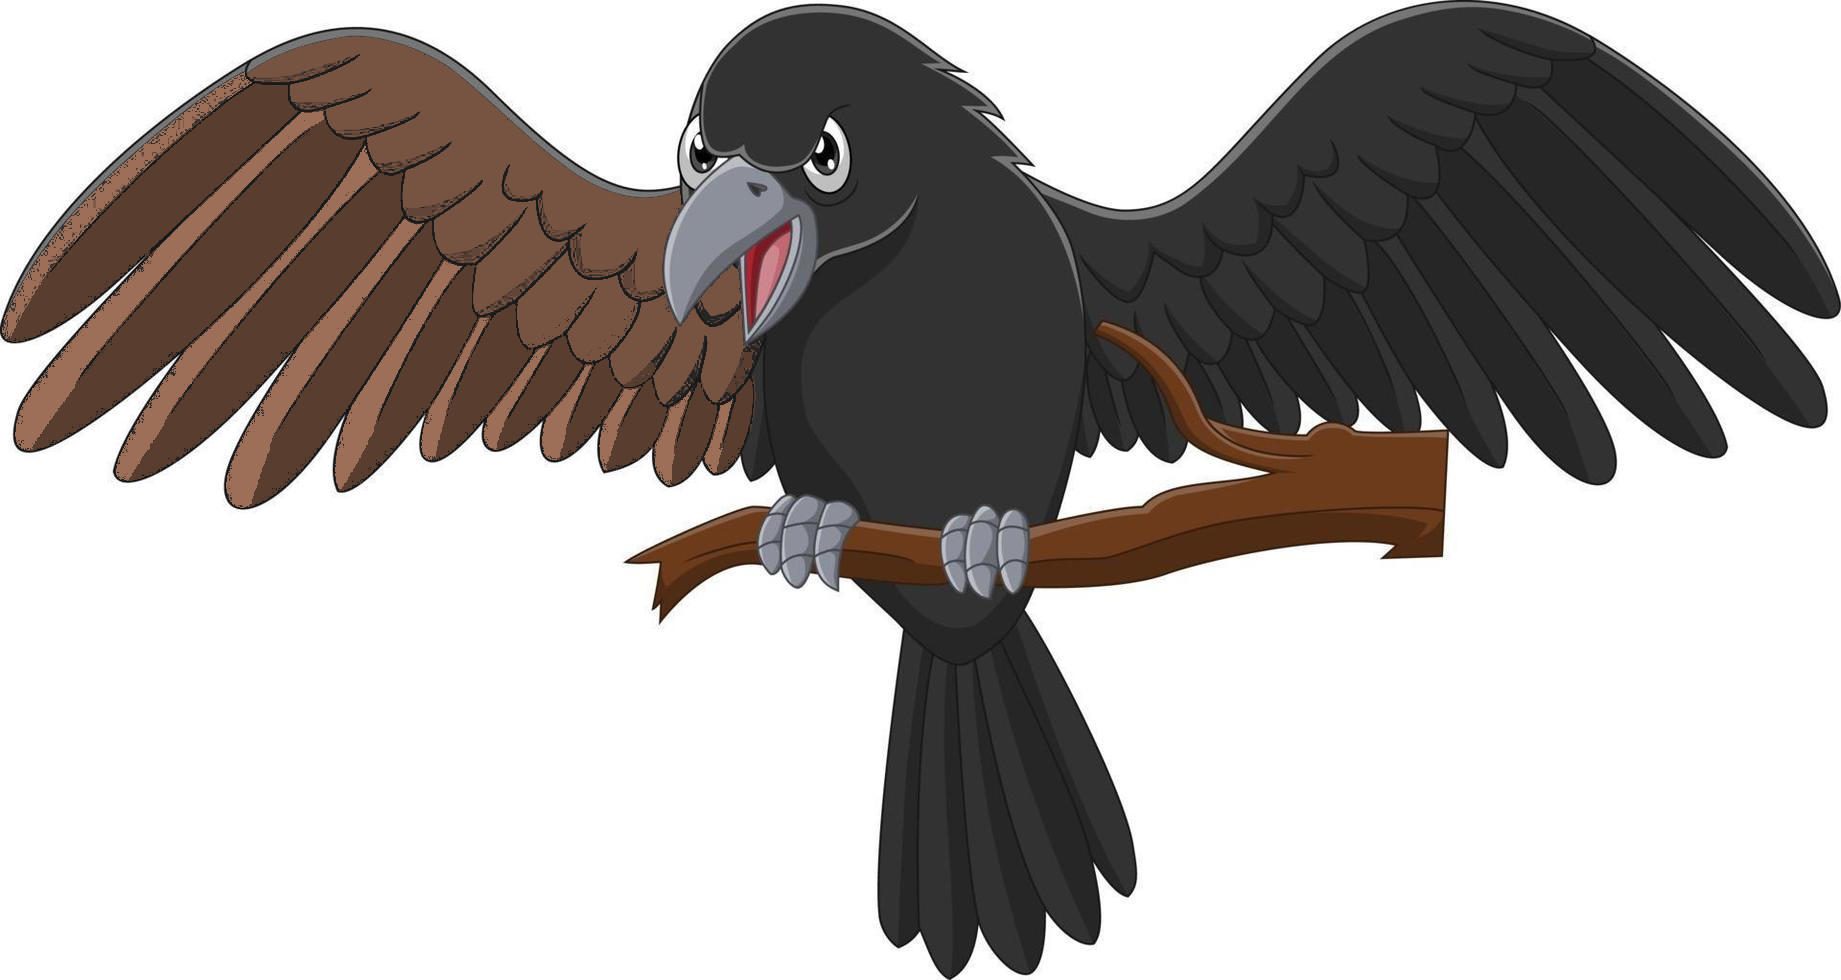
\includegraphics[width=250pt]{eaglewing.png}
  \rule{\textwidth}{0in}\par
  {\Large\textit\theauthor\par}
  \vfill
  {\Large\scshape\press}
  \end{center}
\endgroup}
\makeatother

% chapter title manipulation
% padding with zero
\renewcommand*\thechapter{\ifnum\value{chapter}<10 \fi \babylonian{chapter}}

% chapter title display
\titleformat
{\chapter}
[display]
{\vspace{-2cm}\normalfont\scshape\huge}
{\HUGE\thechapter\centering}
{0pt}
{\vspace{8pt}\centering}[\vspace{22pt}
{\pagestyle{plain}}]

% typographical settings for the body text
\setlength{\parskip}{0em}
\linespread{1.09}

% HEADER AND FOOTER MANIPULATION
  % for normal pages
  \nouppercaseheads
  \headsep = 0.16in
  \makepagestyle{mystyle} 
  \setlength{\headwidth}{\dimexpr\textwidth+\marginparsep+\marginparwidth\relax}
  \makerunningwidth{mystyle}{\headwidth}
  \makeevenhead{mystyle}{}{\textsf{\scriptsize\scshape\thetitle}}{}
  \makeoddhead{mystyle}{}{\textsf{\scriptsize\scshape\leftmark}}{}
  \makeevenfoot{mystyle}{}{\textsf{\scriptsize\thepage}}{}
  \makeoddfoot{mystyle}{}{\textsf{\scriptsize\thepage}}{}
  \makeatletter
  \makepsmarks{mystyle}{%
  \createmark{chapter}{left}{nonumber}{\@chapapp\ }{.\ }}
  \makeatother
  % for pages where chapters begin
  \makepagestyle{plain}
  \makerunningwidth{plain}{\headwidth}
  \makeevenfoot{plain}{}{}{}
  \makeoddfoot{plain}{}{}{}
  \pagestyle{mystyle}
% END HEADER AND FOOTER MANIPULATION

% table of contents customisation
\renewcommand\contentsname{\normalfont\scshape Contents}
\renewcommand\cftchapterfont{\normalfont}
\renewcommand{\cftchapterpagefont}{\normalfont}
\renewcommand{\printtoctitle}{\centering\Huge}

% layout check and fix
\checkandfixthelayout
\fixpdflayout

% BEGIN THE DOCUMENT
\begin{document}

% Mayan
\def\mayaexpansion{%
	\mayacntc=\mayacnta\mathbfont
	\ifnum\mayacntc=0 0\else
	\rotatebox[origin=c]{-90}{%
		\loop\ifnum\mayacntc>5\advance\mayacntc by -5\repeat
		\the\mayacntc\mayacntc=\mayacnta
		\loop\ifnum\mayacntc>5\advance\mayacntc by -5 5\repeat}%
	\fi}%
	
\newenvironment{localsize}[1]
{%
	\let\orignewcommand\newcommand
	\let\newcommand\renewcommand
	\makeatletter
	\input{bk#1.clo}%
	\makeatother
	\let\newcommand\orignewcommand
}	
	
\pagestyle{empty}
% the half title page
%\halftitlepage
\cleardoublepage
% the title page
\titleM
\clearpage
% copyright page
\noindent{\small{This novel is entirely a work of fiction. The names, characters and incidents portrayed in it are the product of the author's imagination. Any resemblance to actual persons, living or dead, or events or localities is entirely coincidental. \par\vfill\noindent Revision 1 Edit.\space\today\\ISBN\space\ISBN\\\copyright\space\theauthor. All rights reserved.\par\vfill\noindent\theauthor\space asserts the moral right to be identified as the author of this work. All rights reserved in all media. No part of this publication may be reproduced, stored in a retrieval system, or transmitted, in any form, or by any means, electronic, mechanical, photocopying, recording or otherwise, without the prior written permission of the author and/or the publisher.\par}}
\clearpage

% dedication

%\itshape{\noindent{Dedicated to my all {\fontfamily{cmr}\selectfont\LaTeX{}} users.}}



% begin front matter
\frontmatter
\pagestyle{mystyle}

% preface
\chapter*{Preface}

This is the first out of two external revisions. So---although, I'd appreciate comments regarding grammatical errors, sentence structures and formulations---the focus is intended to be on the consistency of the story, the flow of the writing, the entertainment to the reader, and, most notably, the quality and feasibility of the book.

There will be, if this first one goes well, a second revision, where the focus will solely be on the language.

I've made an effort use British spelling and British words where there are multiple possibilities. E.g. brook over creek, autumn over fall, rubbish over trash.

Notably I've chosen to use whilst and amongst as the conjunction, preposition, adverb, and while solely for the verb. Similarly, I've chosen to use the somewhat increasingly archaic verb form of but. \\

This story is a satire; therefore, it touches on many ideas and references that is not entirely self contained within this book. It is my wish that the story is in itself self contained(in the same way Animal farm is self contained, albeit very boring if no association to the real world is allowed). However, much of the fun(or value) in reading it comes with the understanding of symbolism and the mockery within it. 
As part of this first revision, I've noted every outside reference(those that are intentional at least) made in this work. I do not want to rely on obscure knowledge of trivia however, and those references should not harm the experience of reading---if so, they should be removed. Please note every reference you are able to find---even the ones that are almost too obvious.
I've divided every outside reference in to three categories.\\[1cm]

\textbf{Category tier one, must be noted.}
Contains very few but obvious references that I think should be known by 80\% of the populace aged 18 or over. They are also imperative for the tale itself. Failing to understand these would make a really dull read.\\[1cm]

\textbf{Category tier two, may be noted.}
Missing to draw these connections should not interfere with the cohesiveness of the tale; they should be passed over without the reader feeling a sense of missing out. Understanding none of them would probably diminish the reading experience.
Most references are in this category.\\[1cm]
 
\textbf{Category tier three, unlikely noted.} 
This category contains all obscure references. They must be completely passed over with no hiccup, i.e. you'd never guess it's an reference if not told so. Some of these require some deduction, and I hope that even if they're found, It's not obvious that I put it there intentionally.

Perhaps unnecessary remark 1: the chapter quotes are carefully picked and are all relevant to the chapter's text.

Perhaps unnecessary remark 2: the character names are carefully picked and are all relevant to the story(albeit some more than others).\\[1cm]

Chapters:\\
1: Intro\\
2: Build up\\
3: Build up\\
4: Pay off\\
5: Neither\\
6: Pay off\\
7: Build up\\
8: Build up\\
9: Pay off\\
10: Neither\\
11: Neither\\
12: Pay off\\

Chapter 1\\[1cm]
c3: Darwin quote, hints to a tertiary theme of the book: [redacted].\\
c3: published in 1859, it fits perfect being ruffly 10 years before la belle epoque.\\
cX: I'm a fan of Darwin's work\\
c2: 'Natural checks and balances': a very darwinian sentence.\\
c3: Locks of gold --- Goldilock: both: https://en.wikipedia.org/wiki/Goldilocks\_economy, and https://en.wikipedia.org/wiki/Circumstellar\_habitable\_zone\\
c3: The beautiful era: La Belle Époque: https://en.wikipedia.org/wiki/Belle\_Epoque\\
chapter 2 \\
will be filled after you've read it.
%Ongenþeow
%Týs öttungr

%Óttarr

%Hroðulf
%Hrēðel

%Αίσωπος
%Αἴσωπος

Characters:\\[1cm]
Introduced Chapter 2:\\[0.1cm]
Kraerion(main, introduced),
Aequitus(main, introduced),
Br'er Rabbit(mentioned),
Ongenþeow(mentioned),
Pietus(support),
Veritas(support),
Cinnamon(mentioned)\\[0.1cm]

Introduced chapter 3:\\[0.1cm]
Kraerion(main),
Redrill(main, introduced),
Greyhead(support, introduced),
Spinestack(support)\\[1cm]

Introduced chapter 4:\\[0.1cm]
Kraerion(support),
Eaglewing(main, introduced), 
Hroðulf(main, introduced), 
Αίσωπος(main, introduced),
Aequitus(mentioned),
Pietus(mentioned),
Br'er Rabbit(support)
\\[0.1cm]
Main: \\[0.1cm]
Kraerion(2, 3, 4)\\
Aequitus(2)\\
Pietus(2)\\
Veritas(2)\\
Cinnamon()\\
Br'er Rabbit(4)\\
Eaglewing(4)\\
Hroðulf(4)\\
Αίσωπος(4)\\
 \\[0.1cm]


Enjoy!


% acknowledgements
%\chapter*{Acknowledgements}

% table of contents
\clearpage
\tableofcontents*

\clearpage

%\pagenumbering{roman}

%\vspace*{4.3cm}
%\begin{center}
%	\begin{localsize}{10}
%		In memory of Richard Adams\\
%		\begin{quote}
%			“My heart has joined the Thousand, for my friend stopped running today.”
%			\begin{flushright}1920 -- 2016\end{flushright}
%		\end{quote} 
%	\end{localsize}
%	\vspace{1cm}
	
%\end{center}

\clearpage

\vspace*{4.3cm}
\begin{localsize}{10}
  \begin{quote}
    “Some people talk to animals. Not many listen though. That's the problem.”
    \begin{flushright}- A.A Milne \end{flushright}
  \end{quote} 
\end{localsize}
\vspace{1cm}

% begin main matter

%“The struggle of man against power is the struggle of memory against forgetting”

%If the misery of the poor be caused not by the laws of nature, but by our institutions, great is our sin.

%The last capitalist we hang shall be the one who sold us the rope.

%Money is a formal token of delayed reciprocal altruism.

%To know that we know what we know, and to know that we do not know what we do not know, that is true knowledge. 

% under suitable conditions, cooperation can indeed emerge in a world of egoists without central authority. Robert Axelrod

% Thus, under suitable conditions, cooperation based upon reprocity proves stable in the biological world.

% “The hardest thing to explain is the glaringly evident which everybody has decided not to see.” ayn rand

% “In man's struggle against the world, bet on the world.” Franz kafka
% “I dream of a grave, deep and narrow, where we could clasp each other in our arms as with clamps, and I would hide my face in you and you would hide your face in me, and nobody would ever see us any more” Kafka

% “If a man does not keep pace with his companions, perhaps it is because he hears a different drummer. Let him step to the music he hears, however measured or far away.” - Henry David Thoreau

%“Communism is not love. Communism is a hammer which we use to crush the enemy.” - Mao Zedong

%"To read too many books is harmful. " - Mao Zedong
% “The more I read, the more I acquire, the more certain I am that I know nothing.” - Voltaire

%“The average man is both better informed and less corruptible in the decisions he makes as a consumer than as a voter at political elections.” - Ludwig von Mises

% “'Emergencies' have always been the pretext on which the safeguards of individual liberty have eroded.” - Friedrich August von Hayek

% “I have never made but one prayer to God, a very short one: Oh Lord, make my enemies ridiculous. And God granted it." - Voltaire

% “Until they become conscious they will never rebel, and until after they have rebelled they cannot become conscious.”  Orwell

% “The society that puts equality before freedom will end up with neither. The society that puts freedom before equality will end up with a great measure of both” Friedman

% “Hell is truth seen too late.” 


% “Virtue is more to be feared than vice, because its excesses are not subject to the regulation of conscience.” Smith

\mainmatter
%\pagenumbering{hexadecimal}
%\renewcommand*{\thepage}{\hexadecimal{page}}

% Or how to pursue the stuff of dreams.
% Or how to get lost in the aggregate.


\chapter{Deordination}
\vspace{-1.3cm}
\begin{localsize}{10}
	\begin{quote}
		"Man selects only for his own good; Nature only for that of the being which she tends."
		\begin{flushright}- Charles Darwin\end{flushright}
	\end{quote} 
\end{localsize}
\vspace{1cm}

The Wadborough forest is a peculiar collection of trees; it's shaped by an improbable set of circumstances, setting the preconditions of this unlikely tale you're about to read. % shaped by an equally peculiar set of circumstance; setting the unique condition of this unlikely tale.

The forest has stood where it now stands for millennia, but surrounded by other trees and part of a much larger forest: it did not crave attention, nor require distinction by name. With the ever increasing sophistication---and population grow- th---of the main British isle, most trees were cut down for timber, and the woodlands were slowly turned to grazed meadows and tiled farmlands. The trees near the little village of Wadborough would most certainly meet the same fate, if it wasn't for a growing posh ritual of high British society. The Duke of Worcestershire---lest he lose pace with his peers---began importing pheasants to be hunted by his guests and his more distinguished subjects. He thus proclaimed that the trees near the Wadborough village would never be cut down, and ever solely be allocated to the hunting of game. These trees became the Wadborough forest---standing tall and alone in the wild ocean of fields.

Pheasants are clumsy birds---used to roam the Asian steps undisturbed by predators---and found it difficult to survive in the forest. To protect their precious game: the Duke's men drove, over the years, all major predators out of the region. The red fox was first to go(to the chickens' rejoice) as they seemed almost offended by the ease of hunting pheasants. The weasel family: the stoat, the wolverine, and the mink; followed shortly thereafter. The badgers were also hunted, but they soon understood that the pheasants were off limit and began to ignore the foreign bird; thus, a few badgers remained alive. As with all human interventions: they're seldom without unforeseen consequences; the rodent population boomed; which, incidentally attracted more birds of prey to the region. These birds---mostly consisting of various hawks and species of owls---did not danger the life of pheasants; however, they possessed another threat entirely. The ornithologists of the time had a fierce reputation of enacting conservation legislation; the rumor of the birds broad prevalence reached the group and soon they took interest in the forest. The Duke thus had a choice: spare the birds and risk the ornithologists' influence, or kill them and risk the outbreak of rodents; he chose the latter. The rodents did explode in numbers, but they did not carry disease with them, nor overrun the neighbouring fields and the Wadborough village. As a matter of fact---the rodents did not at all conform to the behaviours so often attributed to them. No one could explain why.

Eventually the time of serfdom met its end; and the society slowly morphed into something approaching the appearance of a representative democracy. Ownership of land transferred from lords and ladies to the establish municipalities, and so too did the ownership of the Wadborough forest. Although hunting remains a tradition of the well-off, its clientele slowly shifted to in time mostly consist of ordinary rural villagers.   
Innovations in agriculture and growing manufacturing greatly shifted the populace from rural to urban. The growing cities lost touch with the rural arts. Hunting---especially when performed as sport as it is with game---became viewed as cruel and barbaric. The urban population greatly outnumbered its rural counterpart in voting power; activists rallied and tallied support---the Bill of The Wildlife Preservation Act soon passed through the county of Worcestershire; which, conveniently holds the legislative power in Wadborough. The Act contained many a paragraph, but only one concerned the Hunters of Wadborough. 

\begin{localsize}{10}
	\begin{quote}
		'A person shall not hunt game birds including but not limited to the Common Pheasant, Grouse, Goose, Turkey, Duck or Pigeon by means of firearm, or any form of projectile, unless bread in captivity under permission from a state licensed breeder(§95b). A person guilty of offense under this Act shall be liable on summary conviction to a fine not exceeding 5.000 pound sterling.'
		\begin{flushright}- §68, The Wildlife Preservation Act\end{flushright}
	\end{quote} 
\end{localsize}
 
The Act angered the villagers; "what does city folk know of hunting!?" could be heard at the local drinking holes. Wild conspiracies was liberally spread along with wild guesses on the probabilities of actually getting caught. To the villagers dismay, the city clerks had foreseen their unwillingness to abide by the new law and were ruthlessly prepared to hand out many a salted fine during the first year of the bill's passing. 

And so it came to be that the forest of Wadborough was free of both predator and man alike---undisturbed by the natural checks and balances that keeps the order of things. Even the locks of gold couldn't compare to the beautiful era that would follow.



\chapter{Doubt}

\vspace{-1.3cm}
\begin{localsize}{10}
	\begin{quote}
		“I have never made but one prayer to God, a very short one: Oh Lord, make my enemies ridiculous. And God granted it."
		\begin{flushright}- Voltaire \end{flushright}
	\end{quote}
\end{localsize}
\vspace{1cm}


"One day is today---", Kraerion whispered to himself as his tired eyes slowly widened to an open state. The chimpunk had woke---like all mornings---to a loud unpleasant banging sound, echoing around the run outside the comforts of his small burrow. The sound carried with it the news of a new day, and with it: the message that all who wanted a day's pay ought to drag themselves to the great hall, the Aorta, presently. The frowsty air this deep underground usually made him rise as soon as he woke---to seek a more pleasant ambiance---but today he lingered in thoughts.

"One day is today.", he repeated, to reassure himself and still his doubts, as if repeating the words would make them more true. The power of inertia is strong; Kraerion full well knew of its insidious nature: that tomorrow and never were but equal measurements of eternity. He had longed---even dreamed---for this day to come for as long as he could remember; so he wondered why---now when the day was finally here---he had so suddenly lost his strong convictions.

Chipmunks may be genetically poised for a life underground, but not the chipmunk Kraerion. Even as a little kitten, he had loathed their exists: the damp runs and burrows, the second-hand air, the ever present darkness, and about everything else underground just by association. He hated---as only an adolescent can hate---that which most of his peers called home.
Instead, he wished for a strong wind in his fur, sunlight that uncovered all the beauty that is Nature, but most of all the chaotic buzzing of life above, that so contrasts the routines down below. He yearned to run the branches of trees, not the ever branching network of runs dug in the forest soil. His father had many a time japed that his son was born more a squirrel than chipmunk---and he had not been wrong. When he was younger, he had stated that one day he was going to live amongst the trees, but received feedback which would otherwise only be appropriate after a well executed joke.

Kraerion eventually mustered the will to rise from his moss coated bed. He went over to a corner of his burrow and began scratching away at the dirt.

"Good, still here.", he confirmed anxiously, as the felt the steel of seven steel screw-nuts---which would surely appear beautiful in the sunlight---laying before him. He covered them up again and left his burrow into the run, and followed its twists and turns until it widened into a great hall: the Aorta. It was dug under a great willow; its massive network of roots---intertwined with the walls and ceiling---supported the weight of the dirt and kept it from caving in.\\

Since the time of Man, the forest had steadily increased its economic output. One of the  contributing factors was the increased specialization of its inhabitants. Whilst many a specie have some certain advantage in the gathering of some specific type of feed, none is as great a carrier than that of the chipmunk. In their elastic cheeks, they are able to carry loads of feed---and other goods for that matter---efficiently around the forest; their small size and great numbers gave the operation a granularity to it, which made it difficult for larger and stronger animals like the roebuck to compete. When other animals began to hire them for their service, they began to expand their network of tunnels and runs to cover whole forest---connecting all its major hubs. Therefor---every morning---the chipmunks gathered in the Aorta to share news and plan the day ahead.

Most chipmunks were already present when Kraerion entered. 

"One day is today.", he thought again, as he headed towards his usual spot in the front. But he hesitated suddenly and reconsidered; instead, he decided to begin his new life with breaking this habit and found a place in the back.\\

The murmur of conversation disappeared in an instance when an old chipmunk appeared in the Aorta. His name was Aequitus and was the chief chipmunk, gray spots of fur spoke of his age, yet his features were easy on the eye and he bore his age proudly. Everyone knew the chief and saw him as something akin to a revered hero. When he was but a kitten, he'd taken interest in the chipmunks' livelihood and noticed irregularities in their billings; after some further deliberation with his friend Br'er Rabbit, he realized that they could likely double their prices with little to no churn. He put forth the motion to the then chief chipmunk, who surprisingly listened to the youngster and approved it. When their income subsequently increased, he was very vocal about its occurrence, and made it impossible for the chief chipmunk not to pass it forward to the chipmunks' daily wage.

When Aequitus a few years later became unanimously chosen as the next chief, he took it a step further. He transformed the chipmunks' enterprise to a sort of cooperative, with bylaws dictating that a fixed percentage of the total revenue would be earmarked for workers' wages. As well as other rules limiting the influence of his own office---not only for himself but setting the precedence for his eventual replacements. 

Together with Br'er Rabbit---who had by then become the implicit leader of the rabbits---and with the help of the by  then Glade of Representatives Twig Ongenþeow, he started the Winter Fund. A collective fund that functions similar to that of human insurance: its members contributes feed during the spring, summer, and autumn as a premium; members that find themselves short during the winter may then make a claim and receive feed to sustain them until winter's end. % Dearth

A cynic human might proclaim the flaw in this scheme, that an animal might take advantage of it by wasting his wage and making a claim every winter---but he forgets two things: most animals can't count; and although possible, making a claim is very stigmatized, and that most animals would rather starve than to broadcast their destitution. Aequitus also---being a co-founder of the fund---made sure that all the work related to the logistics---moving and storing of the feed deep underground, where the soil is grainy, cold, and preserves the feed from pest and rot, and hidden from prying thieves---went to the chipmunks---further boosting the demand for their services.

The fund was a great success; winter deaths decreased drastically the first year, and then slowly year after year. The chipmunks got a more steady stream of sophisticated work from the fund and thus means for a better life. For all the contributions Aequitus made, none could match the feeling he instilled in every chipmunk: the intangible sense of worth; the standing the brought them to in the forest; and the care he fostered between chipmunks by treating them all as equals.\\

When Aequitus reached the front of the Aorta, he turned and faced the scurry.

"Before we go through today's agenda, I have news---both good and bad.", he began, "And, as you may not be able to appreciate the good in anticipation of bad, I'll begin with the bad.", he took a tactful pause, as anyone with his level of experience would in this situation.

"The eastbound run collapsed late last evening; we're completely cut off from the eastern part of the forest. Therefor, the deliveries to the rabbits' hill must be postponed."

"Why did it collapse?", Aequitus younger brother Pietus asked, who stood at his regular place just right of his brother.

"Well---", Aequitus dragged, "a pheasant went chasing a maggot again and crossed above the shallow no-zone."

"Again!?", Pietus cried, not hiding his contempt, "Did the pheasants not promise to be more careful---that last time would be the last? Will they honour our agreement and pay for the damages?"

"They did indeed. As you all know, the pheasants are not the most organized of animals and will only blame each other if we make a claim for damages. We may bring it to the Glade, but what---other than appearing petty---would we gain? Little and less, I'm afraid. Nevertheless, I want you, Pietus, to go to the moles and have them dig a deeper eastbound run this time---that is, at least, a factor we can affect."
"I'll do it.", Pietus responded, "But send someone else to the moles next time---they don't even speak our language..." %the common tongue.

"Nā, hēo seċġaþ þone ealda sprǣċe. It is we that don't speak theirs.", Aequitus paused, waiting to see if Pietus had a response. When his brother only mumbled something inaudible, he continued.

"I'll make sure Br'er and the rabbits get the news of this postponement personally. As for the good news, the rumors going around are true: the Glade have decided to institute a 2\% tax on all Forest shipments. It's only a temporary experiment with us as the pilot service."

"How is this good news?", Veritas squeaked, a tiny runt of a chipmunk who were also standing in the front close to Aequitus.

"Two reasons: firstly, the funds are marked as aid for destitute animals who can't afford the Winter Fund, and we'll surely get the contract for its operation; secondly, we don't pay for our own services---we're essentially exempt!"

"No! That's not how it works.", Veritas snapped angrily, "this will force an increase in our prices---hurt our margins; to only burden one industry, and ours at that---it's... it's incredibly unfair."

"Enough.", Aequitus grumbled, "That's enough, this is neither the place nor time, we may discuss this later in private."

Veritas did not answer, but she turned her head sideways---showing everyone her disdain.

The old chipmunk moved on to the day's normal agenda, dishing out more routinely orders before dismissing his workforce. However, his eyes were fixed on Kraerion---the dismissal did not apply to him. When the last chipmunk had left the Aorta, he began to speak.

"Kraerion---", he said.

"Father.", Kraerion responded, equally enthusiastic.

"It's true then, hiding in the back like that; you're actually leaving what we worked so hard to create?"

"What you created you mean? You cannot pretend this is news---I've been more than forthcoming with my intention to lead a different life. You of all chipmunks should know of my extra shifts to afford this move, and my refusal of the managerial responsibilities you so blatantly pushed on me."

"We all have dreams, Kraerion. I know you might \textit{feel} like a squirrel, but you're not one---I promise you that you'll end up miserable, dearth of resources, and completely alone in a world of wings if you try to live as one.
Dreams are a lesson in growing up: learning how to smother them in favour of what's truly important in this life. And, you'll get other dreams---realistic dreams---like forming a family, building a future for our specie, and contributing to the betterment of the Forest at large."

"I'm sorry---", Kraerion said at length, "but that's not me, and quite frankly, that'll never be me."

"Don't you feel any sense of responsibility? What about your sister Veritas? You expect Pietus and I to go on forever?"

"What about her? She's smarter than us three combined; she could take over tomorrow if you'd only let her."

"You know full well that intelligence isn't everything. You saw how she acted today: she lacks the social conduct to lead other chipmunks."

"Maybe you should have spoken with her before announcing your decision to the whole Aorta?"

"It's not only today and you know it. Never mind. If not for us, then what of you and Cinnamon?"

"Don't", Kraerion said flustered.

"What, you haven't told her!?", Aequitus said truly surprised; he was just about scold his son, but hesitated when he saw Kraerion's face and realized it would be superfluous. Before he had time to say anything more, Kraerion turned around and ran.

Kraerion ran, and he ran, and he kept on running until the pain in his lungs, and muscles, numbed the thoughts that so rudely had occupied his mind.

\chapter{Dread}

\vspace{-1.3cm}
\begin{localsize}{10}
	\begin{quote}
		"'Emergencies' have always been the pretext on which the safeguards of individual liberty have eroded."
		\begin{flushright}- Friedrich Hayek\end{flushright}
	\end{quote} 
\end{localsize}
\vspace{1cm}

\renewcommand*{\thepage}{\footnotesize \hexadecimal{page}}

Kraerion eventually stopped running; once his emotions cooled off, he felt embarrassed for how he had acted. 

"Well, good riddance---", he thought, "at least I can't go back now. One day is truly today."

The chipmunk returned to his burrow one last time, to fetch his screw nuts and say his goodbyes. He had stood there for a very long time; not knowing how to say farewell, and he somehow felt that the moment required a solemn pause. When he made an attempt to leave, his legs refused; he felt an annoyance for his own nostalgia. Life underground was all he had known; nothing would ever be the same.

When he exited the networks of runs through the exit known as the Northwestern Arteriole, a large woodpecker were already waiting for him. His name was Redrill, and he had an especially pronounced red crest. Woodpeckers made excellent woodworkers, but most of them worked in small teams and only took on larger construction projects. But not Redrill, he was a loner and preferred to work alone and had hence accepted Kraerion's rather unorthodox request. The seven screw-nuts he had fetched were awkwardly wrapped around his front legs, and caught the sunlight and glimmered harmoniously. 

\renewcommand*{\thepage}{\footnotesize \arabic{page}}

"You're really sure about this?", Redrill asked.

"Yes!", Kraerion answered, maybe a bit too quickly, as if he was caught with his paw down a honey pot, "I---I mean, I've never been more sure."

"Don't worry,", Redrill chuckled amused, "I won't argue with the hand that feeds me. I see you've brought payment."

"Well, only one is for you though. Better get going."

The woodpecker smiled, nodded, and unfolded his wings and set off north with Kraerion---with all his might---trying to keep up the pace through the thick undergrowth.\\

The Wadborough villagers---in a time before environmental concerns---dumped much of their \textit{undesirables} in the forest. Everyone denied it---of course---yet batteries, plastics, electronics, and everything else one can imagine found itself in every nook and cranny of the forest floor. Even a run down car or two occasionally joined the detritus. Most animals---after a good whiff---would not bother with these alien contraptions. But, in a magpie a curiosity grew; soon, he conjectured: these objects of Men may teach a thing or two! The magpie began to take them apart; study their intricate design and their innate structures. He felt an unnatural compulsion towards to the weird family of human fasteners: the screw nuts. Death may be the mother of all beauty, yet these imperishable hexagons of cast steel were of different kind. Sun rays bouncing off their plain silver surfaces caught the magpie in awe; the beauty consumed him, and he eventually took to hoarding. The desire for these little things spread like wildfire; first amongst the magpies and the other birds in the crow family, but soon all animals had taken a fancy to them---a treasured commodity was born. But it wasn't like any other commodity: it endured where blueberries rot, it was portable where trees stood firm, but most significant was its limited supply---a thing of Man. It couldn't be produced like the spines of a hedgehog's back, nor grown like the acorns of an oak tree. Naturally, the young economy was tired of barter and sought a system to keep better score: an informational instrument to keep track of favours; a fair system of time allocation. And thus, for the first time in the kingdom of animal, go beyond reciprocal altruism---transcend death---and let a money be born.  

But to Kraerion, the screw nuts were but a means to an end: to purse life anew. \\

The day was a beautiful one; the sun shone bright on a blue canvas sky with only a few dots of white. His seven screw-nuts around his legs made it difficult to run, and he soon lost sight of Redrill. He did not worry though, the woodpecker would not drop his client for a lousy tempo. His anxious feelings from earlier that morning eased somewhat by the fine weather, like the miraculous cure weather so often can be. 

"What a great day!", he said out loud to no one in particular, "What a shame it would be to have it spent underground."

The sun's rays told of high noon, yet the forest was uncharacteristically quiet. Noon was a time of activity, when the animals left their nests, burrows, lairs, and vocational duties to seek out trade. To buy or sell feed; to offer or acquire service. Anything imaginable were up for sale: a blackbird could be hired to sing, a joyride could be enjoyed from the back of a magpie, fresh blueberries---or stolen cabbage from the neighbouring fields---could be bought. Therefor, on any other day, a distant voice in his ears would not have sparked his curiousness. When he reached a clearing in the trees, he leaned back on his hind legs and saw---past the overgrowth---a hedgehog and a robin arguing intensely. He recognized the hedgehog as a acquaintance of his fathers, he knew him as Spinestack, and closed the distance to them.

 "Are you mad?", the robin asked flustered, "Have you completely lost your mind? You know I need more than two measly spines."
 
 "Spines are not weeds you simply pluck from a field of your choosing; they take effort and care to grow.", Spinestack answered calmly, "And these recent---although tragic---events have created a wonderful demand, as you surely understand."
 
 "But... But that's more than trice as expensive than just a couple weeks ago. This is war profiteering! I'm down to my last screw nut; you must understand."

"I mustn't anything.", Spinestack reassured calmly as he saw Kraerion approaching and waved, "I could ask any of your neighbours, who, I'm sure, would find the price both fair and appropriate."

"Wait, hold on,", Kraerion interrupted as he took notice of the small heap of spines, sharp and keen, laying between the two animals, "What do you mean war? And what on earth would you need spines for?"

"Oh haven't you heard!?", the robin squeaked, "It's terrible---\textit{Terr-i-ble} I say: just this morning a nightingale in the same tree as me got her screw nuts stolen. And it's not an isolated incident either, it has happened all over the forest in the last few days. I refuse to sit idle by; we must take up arms and defend ourselves---just like in the tales of the time of Man!"

"Hrmf", Redrill uttered from a twig above the group, seemingly appearing from nowhere, "I heard a few rats have similar complaints earlier this morning, apparently a few of their burrows had been raided. And they are \textit{rats} after all, who dares mess with them?"

"Yes, very sad indeed. Now could you take your discourse elsewhere?", Spinestack said glaring at the two newcomers, "We are conducting serious business here, go waste someone else's time---preferably someone whose time is of less value than mine."

Redrill gave Spinestack a sharp look of disgust, "You've always been more heap than stack, don't you think?", he jested, untucked his wings, and took off. Kraerion had not much choice but to follow.\\

When they reached the silver birch---which was to become Kraerion's home---a fluffy wood pigeon greeted them with a coo. 

"Welcome Kraerion, to our humble and peaceful corner of the Forest.", the pigeon said. His name was Greyhead; this pigeon landlord owned a score of birches and had agree to sell part of one to Kraerion. It was very unusual for one animal to only own part of a tree; most animals paid rent. Kraerion had first been offered to rent, but refused---he was ready for a life free from the burden of economic dependence and thus the need of a steady wage.

"The meter directly above the first twig is yours. I've etched in some markings, you may, of course, measure it yourself."

Kraerion nodded and handed over three of the screw nuts to Greyhead. The pigeon thanked, and having errands elsewhere---excused himself and flew away.

Redrill had received instructions many days ago, and wasted no time consulting Kraerion on what to do. He flew up and landed on the south facing side of the birch and began drilling. The woodpecker's head jerked back and forth, transforming his appearance into a red smear. Kraerion felt very silly when the origins of Redrill's name suddenly dawned on him, he could not believe how he hadn't realized it sooner.

Woodpeckers were not made to carve homes in the trunks of trees. Their strong chisel-like bill and shock-resistant head had slowly been selected by Nature for its ever increasing ability to prey on termites, beetles, and various other larvae dwelling behind bark and wood. But---like most animals---with the rise of a market, their abilities found a vastly greater commercial value elsewhere. And, the woodpeckers found it in carpentry.

Kraerion didn't know how to act whilst Redrill worked. He felt that he would only be in the way if he tried to help, and there was nothing else there he could occupy himself with. He had not stood there long before he was saved by a loud screech from a neighbouring birch.

"Wait here.", Redrill yelled urgingly from up above; he dashed---without hesitation---towards the sound. Kraerion paid no heed; instead, he lunged to the tree and rushed up its trunk. The trunk divided evenly into three large limbs; between them lay a pigeon's nest. He continued up one of the limbs as to look down and see it. Redrill was perched on a branch opposite of Kraerion---they were the first on site. And as pigeons came flying from all directions, they looked down and saw a terrified mother and her three newborn squabs, naked save for their scrawny, near undeveloped down.

"They're gone;", she said despondently, "They're all gone. Oh dear, how will we survive?"

"Won't nest insurance cover it?", a pigeon asked after a long moment of silence.

"No,", another pigeon answered, "theft has not been an issue since the time of Man. Why would anyone even think of including it in coverage?"

"It may yet be rectified, as far as I'm aware, nest insurance has always been implied to cover these kinds of things. I'm sure there's some broad clauses in there that might be stretched to cover this situation.", Greyhead broke in, sighed, "Otherwise, we'll come together and cover it ourselves; solidarity is not yet lost on us. Regardless, the best we can do for now is to give her some room and time to breath, especially by those not yet part of our community."

The insinuation was not lost on either Redrill or Kraerion. Nevertheless, it was a reasonably request, and the two animals vacated the tree.

"We're not particularly popular today.", Redrill muttered jokingly. \\

The moon had long since appeared when Redrill finished his work. The woodpecker sailed down to Kraerion at the foot of the birch.

"I guess I'm done!", he proclaimed, "Are you sure it's deep enough? It's barely more than an entrance."

"Well, you know I can't afford more of your time.", Kraerion answered. "Besides, me teeth should be strong enough to carve out the rest. Take the screw nut before I regret it."

As he handed over one of his screw nuts to the bird, Greyhead appeared again.

"Good evening, excuse my rude remark earlier," the pigeon began, "these are strange times; I hope you don't take it as a reflection of your person."

"No offense taken.", Redrill said whilst Kraerion simply nodded.

"I have some news that might not have reached the two of you yet.", Greyhead continued, "The crows have called for a state of emergency, there's going to be a meeting in the Glade, tomorrow at noon. Thought you'd like to know."

"Okay, thanks.", Redrill said tiredly, yawned, and turned to Kraerion, "It's getting late, are you sleeping here?" 

"Not like I have a choice, the new tenants have most likely already moved in to my old burrow."

"Well then,", the woodpecker said and untucked his wings, prompting Greyhead to do the same. The two birds took off and disappeared into the blissful summer night. Kraerion was left alone with his hollow, his new life, and his ever intruding thoughts. Still unsure if he had made the right decision, he climbed up the tree to his entrance.

"One day was today.", he concluded solemnly. The hollow's floor was still rough and unyielding, but it wasn't the brown soil of a burrow---that was all that mattered. With time, he would widen the hollow, grind the walls and floor sleek, carry up moss and lichen to make a bed, and slowly be able to call it home. That night, he slept uneasy; his body and limbs were heavy and exhausted, yet his mind was unbridled and completely awake. When sleep finally came, it was with an unusual satisfaction that only major life decisions produces---it scared him to know that he'd almost gone a whole life with- 
\newpage
\setcounter{page}{15}
out it.



%PDF-1.5
%����
6 0 obj
<</Type/Metadata/Subtype/XML/Length 3332>>
stream
<?xpacket begin="" id="W5M0MpCehiHzreSzNTczkc9d"?>
<x:xmpmeta xmlns:x="adobe:ns:meta/" x:xmptk="XMP Core 4.4.0-Exiv2">
 <rdf:RDF xmlns:rdf="http://www.w3.org/1999/02/22-rdf-syntax-ns#">
  <rdf:Description rdf:about=""
    xmlns:xmpMM="http://ns.adobe.com/xap/1.0/mm/"
    xmlns:stEvt="http://ns.adobe.com/xap/1.0/sType/ResourceEvent#"
    xmlns:dc="http://purl.org/dc/elements/1.1/"
    xmlns:GIMP="http://www.gimp.org/xmp/"
    xmlns:tiff="http://ns.adobe.com/tiff/1.0/"
    xmlns:xmp="http://ns.adobe.com/xap/1.0/"
   xmpMM:DocumentID="gimp:docid:gimp:ebc9a219-e906-4f95-afb9-b92856a2bf2d"
   xmpMM:InstanceID="xmp.iid:fddf5208-e36e-42e9-8314-1cf158500f46"
   xmpMM:OriginalDocumentID="xmp.did:f5bb8702-8908-487f-aee3-9d99cd8fcc51"
   dc:Format="image/png"
   GIMP:API="2.0"
   GIMP:Platform="Linux"
   GIMP:TimeStamp="1668317895985170"
   GIMP:Version="2.10.30"
   tiff:Orientation="1"
   xmp:CreatorTool="GIMP 2.10">
   <xmpMM:History>
    <rdf:Seq>
     <rdf:li
      stEvt:action="saved"
      stEvt:changed="/"
      stEvt:instanceID="xmp.iid:cb4b2502-149a-4edd-b708-76566ed4daeb"
      stEvt:softwareAgent="Gimp 2.10 (Linux)"
      stEvt:when="2022-11-13T06:38:15+01:00"/>
    </rdf:Seq>
   </xmpMM:History>
  </rdf:Description>
 </rdf:RDF>
</x:xmpmeta>
                                                                                                    
                                                                                                    
                                                                                                    
                                                                                                    
                                                                                                    
                                                                                                    
                                                                                                    
                                                                                                    
                                                                                                    
                                                                                                    
                                                                                                    
                                                                                                    
                                                                                                    
                                                                                                    
                                                                                                    
                                                                                                    
                                                                                                    
                                                                                                    
                                                                                                    
                                                                                                    
                           
<?xpacket end="w"?>
endstream
endobj
7 0 obj
<</ColorSpace/DeviceRGB/Metadata 6 0 R/Type/XObject/Subtype/Image/Width 1841/Height
980/BitsPerComponent 8/DecodeParms<</BitsPerComponent 8/Colors 3/Columns 1841/Predictor
15>>/Filter/FlateDecode/Length 508874>>
stream
x��}wp\�u�cI�m(�^� @�M��2�-;v����b{2�$�$������I�ȣȖ�X�Ul��%ٴi��DR$EQa;AB����b�XR�w�'{��-@�I��3�������}��{�w�{�|��ǖB�P(
�"
zGs���20w�\,��X��y���]n��Ga��J9��Q�zٌ+y�+W���/.G�Ľ�ϟϕX�����/_��x���9pc|lϏ��`~�ls�w�m�P(��Χ�H�m$ŷȆ$5�*�����\�c~�a���q����^����~?^��0ִ���-,����_n�
�Dp?7����B�N��8���5>>n�;)))55599�.�[�-3.�N��Ϸ�,�s?��kl����T���d/������z

�B�P(l��cd����
*�2l^ܒ��J8FKy@3�KM�8��3D�%G0õ�>",X �B��,
[��R���|�ccJ8	�oT(
��S�Z�p!R{?��L��@X\ 
18�-���J�Ksdddxx����;
,�B���|�Hccc8��2��#� �P@xSb�5�^	
���Pҽp��E���OqL���OKKs:�xMOOOMM�z�\�/��.�]M	9cXIC�|ίgƻ�1W��B���P�[�P(
�����B�)�!�R)��HV�jDI��4MQ'��AX��K�n-#֊���]�VyX
N�����l���A�	�U��/_�lE�h(ꘒ#�_��ꝠP(�O
�p�
C��Ƥ!39T�;�� �����t�R]]]OO@j`ᱱ1�
A;�N���#\.<�eC%Sc
�!^�ر��@�,Hd���W���;�9v���d�`j->���dff/Y�$===%%kp4�����ƺW"��1π�{
�4��d
�B�P(~3�Ủ�T_BX	�G�FQ$�32���@O2q�i,x忣����(R�6h���8��.��X�G�'b��Df<��;�,
1���$i�,��
�BqS��'�Jhtxx�qO�)����Y&�vtt�|���ʁ�������6�ߏ}�P�E"�III����Ą���19/Df�0�T�#H�-V^�|Y�$���4^�-X�O$���H������Ȍ�p?
�ccc`p|����.�ڵ������322<���������󳲲�N'~���������h�M��{O���И�B�P(
�U�U2QfX�=sc*����@ 044����(IK�J,s
u�!����(V��8���M�j�9���-�/_�)D�6�9���Q���z2�oq������k�w1'�VA�P(�O��|et�é����%��G�lll����kkk+�tpp�E�-[���� >	������ʁRIh�^�1I����qHU��5?Š��J�x+ů�*@��_���\��Jؔ!ݞ��
�@���m�`����?��r�����W�X����v�=��a�؊��J2�R�B1mD���R(
�B���I�iɣ������@_��4$d�H;sG��`B��_u*ɭ,*'3�>��ٯ>��A[JD,��@�B����gdd���@ȥ��b��F�gQ���a�W
�B���J�!�p�D._�Ƭ���t�H�̙3CCC`���Q���JNNNHH`�(&IdŎ��[�x����H��%q�P($��e0U�[�Ȼ�5�r@�ɚ��Dl~�豱1�+I3Ʀɹ8����8	�U�p��c������L�fgg��A��~��7��k��B1��1Y�B�P(���d��$àЇ��522������T__�������B2�=V3`v���a1;ί�+��"�"p~��H��(AR�1Y)Y���c����I���X��[H>Z�؊�
h��K���奤�$F�i�%�4,�P(���SG��Y�mmm


UUUxe2,h����29��v;N
1���d�Xl,��8�I��	c��,i�K��2J����.^fL�'1õ�DZ�&��R^��Q�����V��g�0茟�/��=�BHX����r�>99�^^^���f�Ε��r��.�T(�>4&�P(
�B���3%�H���j�HhȚ�������i���ȸ'^9��1Ф�$j0s�����'�4�O6��\�����;p��Afw|���Q6a���!����r+..^�reAAAQQ�\jj*��HPk�ٝ
�B�P|
�������FϞ=���P__����M M���r��A &�K���W���2���HX��͘,hQ��QO+	%o����{�A���'��H�VR�D~��+�����8,��+	�ۓv���O�"e��o��w�ڻ�E�������P(���i���n7�|͚5X���HKKÉ�lY�bZ@c�
�B�P(f2���������X\�5���,-�#���UUUuuugΜ��PD̵�fl��֌ceIꁸ��P�h�Ԋ���
Ks��&���03w���,V�n*������6��999aZ���$d,ae�[&�0���@X����O���v
�bz�6g�t��b�,��6���� ���d.���Pss��s�Ο?�q͑��x:p
S;�ZZſ8g~0�i]�-kv�����h}XFi�W�O'3^��뱆�Q,�8��x����
&�s=|z l��W�].���J�KҮ��<>�<������c��;�����u�֕��._�����eS2�2ç33WΘ�L28��ZZ	A���И�B�P(���!'\��h�"��O��ŋ3�b���>������UVV�={�ҥK�0��b2�ʓ=C$�F��r�d�Ƴ�\E:�T��+=����vW�sQ�D�lV֣�Ïehf�r:$~W__^��d.dEEE^^��	²�.�v�K�陜�II)�_U�B�PLG�d
��qܑɤV$?���H�'�%677755�߿����eFGG� ���,�(�>�$)2 v��)�Z�@'\
��D)`E�!���p��1H~y���Y����1Y+�A(�5�ޚ ś=<�)��]�=�	��`V�L-/��� �����WyyyNNΪU�֬Y�l�2�y�fjKM[~����AY^��)И�B�P(�i�kh��RaREP�Q�-Z�k�O�>]SSSYYy�̙��^���������z�<5$�w(���SV)�m_C4��5��5b�VLX���m�,������X떉0L����$4UK�R���痕��[��.//�����!n��桠�'e��ލ
�B1�����g97��ǀ�v2JҬ���p�¹s�Ξ=[__Ҍ��OMM���LNN�l)��㘑V�&,G�H1�+�~��yd;���q�_�%�T
�z�I ��~Sb�����Y��L��4?���i��7�ŷ��4)��
GKJJ������f�3��f1%\�98���x�ҥ�m��������7�����M�_�c�P|vhLV�P(
Ō3@%\ȾX�Rz������ǎ;y�$�D�ggg@LBϰGE �
�����O�E������W�TDًU�̹�foh�GP2YWϑ��c�6���6�Œeg�f���9�����B.//oŊk׮]�r%�	���=9*�10-�Z�d
�bf�1S)�#qL0���������r�ȑ��zd
c���q�>��Qzs�F��J�
e,S��EY`2,;[b���A)Pp9
,���j��NȪ71&+����d'da+flU�z�i����j��$V��$�NOTWW�}``>�듓�=ϦM�
W�^]RR��0<�8�R����%��W(��U(
�B1c�I�2�ϊ����Ȏ��s��;v���Ð�3�Е��������DJ)rN2w���Ō�ʔ@i�lΑ�"�T�J&�`
��&9�z�A�͍B�-�����Ogy�{�m�9�L������.>>���|�ʕ۶m��^�d	���H�Y馢�Y�B��v*a���F����]SSs�ĉ���w�}w||�	jHKK����`%����c�.e<��W��!�b&,�a	~�	S� -c�>'�بV�UoJLV~�����k��O0��;�:HtZ������H�.�K|�=�T..A8��
mmm���x����QQQ�q��U�V�������/�p�k
�-��d
�B�P�d0�����o(�2�p���ݻ������w�wdee&''CI&&&B�P�09�b��,��$,H-[�f�Ψ+�0�o%i+�*�+���gdf�uu�-�.H2��e{�Y%u褑�d��ه�VK�RY���n7K�A���444��~l���^RR�y��
6���������׵ò�U(�)ɾ*��ן={�ԩS555`�� %%��b9yL��0n(�Ų�f}X)�������8b=㰜����e.��|^�׊I��+�D5>{=�؃[F�֜�"5�����'M��L�7"���q�^/�';bN⑳m6�b8������ۋk_��v������[��F`E+WH*�B��uИ�B�P(�i��Ăy�l�]W[[��;�TVV����*��y=n������Z����kdd��pH_iFN�[�cr�?^���{̇�v�TY���
��-3����F��J��`���]JP�e`�2��c
��GC݋_��5>>��2��R��U4~�7$\kk+>+���֯_�]w�Y�&''��j���&����S(�)�9�L:44t����/?~�ҥK�� в���K�bc���J+2r	b_/��2OV������L�7�ۃ[����L*�V$�aHsz���j�.'��}��3�d�9Ķ��7��
cy�Z�P�
S��h����X���������ŋن�b����Q��s����vvv���p�h}���[�lY�r%h��2��MLVgV�P�4&�P(
�bڃZhB0����z�޽����B0���w�\P )))��RA�@
�8�K�Bm�G�ž�"���X)��I���Wi'b�lj�9k60a^�(ds����������1�^	`��Yi}&�D�DT�jH>�ۍ�A��,^����y��woڴ�������}�	��޴
�B1�9�	"uuuo����@�K�.-,,$G`3�}
�1z�R���Jb5Xa%��G�L����h��Z���M�� /{TZ1�ץV�p����V�\��
B����eF���nF�%v,�dj�4��1��g����X;����8f��C`)|�n��������~�UPPp�]w�{��+V��x<�Ŕ'��*���d�i�ؚ�:n�P(f0��]T)TzL�z.C�`}KK���]�Μ9��������"�؀��B����P�pԄ�.�d��_R��AN	�.��l1_+��ڊ���G�h�"��-�T��a�YD�)y��n__NlGG�4�����-[�|��_�V�ig1;��r���J��3���$���B�P�,����8�ƀ�G�����l	RaWW׉'8����ǾK�,INNNMM}�ɪ J[=�Xn� GG���u~L"�љ�S����(��p�\.R?ɝUz9�������944�ˍk�r�ʊ���[��_��eN.�gYAFe��������:v��%И�B�P(�)�����l����+�Bbb���Xww�ѣG����С��������������4f�H9��Pj�l�WV�Â9aP��ט���8v��dc%.�߂��hY�@�YˌQ�jY2'd``���*�:))�����_��}��WTT�S���8��.�?���!M
�L�P(n8�ɂ<V�&���a䱌�qqq����zP��]�Ν;V�z����0�YYY,P�QI9,�D�ޤh�Ɍ{����2'ԓe���d��W�S�u��d��,��|�v��Τr��444Ym����#TTT,[�l��ͫW��=��'��T\M���3'��-�����S�@1K�1Y�B�P(S��'�vgE��
��~��
h~�����G����~ǰ���˗.]/�g)q4d����0Vb!�#�
��L�i&M�.�W�ԥ��lA��Q���t:��(љ2L0��"\�6���^UU��Ѐ��v�}�=����ׯ�"Mհ1D�)J�}q�壭h��
�
�BqS.`�#�=�X�<��Ǐ�߿��W_
��0�III���999.��ÖV��'�p���+uo���b�~2Ň�#`J��m���e� Ҙ�Mt	-���`�+������kp�%.
�Twww �>��lٲ��X�fM^^���f~4��Q[\A���F�r��
����E���ϩ�8�b���i3Y��B��I`���)r����ȫ�����^ۻwo}}}ZZZiiiII	���t^fJ�}��P��h�m'3E�'��u�}|��|^�����-�r��
0m��t:��4UI�<S�F��O;::Z[[�.��ʕ+���������G`+�dck(�)
�M��	a��@s0�0���������ǎ;y�dSS����*..���`���{�9W�5ȕ�Y�16�^�2�*@$p��՘�-�v�k�v��������ۀeF@Zǖ�u\D��������Ú999��b�
�ۍ;�5�עE���cM�P��b�Ac�
���Zի
�bV^>�s�/#�2BB����_~���^��d��M�6�\.H�
�R��f��Q(���A�
(
��2lZ�i#��)+cwLY������毓I��ѐ�y4���B�ٰ`&IY�(9QDz}}}���P�8��k׮����x���K�2-������
����&��2$ʸ*�����={v���)))EEE+V��DWr�R`T�19���$Fia���P(0Ӗ���4��^BF§����9���KEx9����?	T���,���5� FGG[ZZjjj�������Ն
��瞂����.����u���U�q
��Í>ת{
Ŵ����l{���w��q��1Œ�������\V=�IIIP�K@�

��(aYMO�C���i�!y=f^�Ա�����Z�^�ҹK�E-Se֜e�R6aO0�gk�G5����N ��w����|�+���<��g�>
�Bq�IDe\����y��7�|����`������l���n��Jr��Zb�ە�3V���T`�k�_�e
�4c�§��)�Œ|X����r�̟%׳^?�`|�ϲS��H��kkk/]��[�^QQq�=��}��˖-�Ƽ�^7'�L��J�Y��*3'<!]nt��d,x�b�#V(�¦M���=�J?�����^z��W^9w����]�~}ZZ��ŋ�����aE��X�����Bgg'�
s��ŪH3�JkjH�1S-�c��^��!�N�h�
s[�Z��ga�0��@t4XVV��?2a����4,A���m�:����w۶m���w�l��p8b��)cyM�B�P(n�߆]e����D����s����h�z,Y���v���1��&��`�td^��(-���~�xxkH6g�|�1N�d�1�Dc�7�jx�8\�S-�%Vˑf�Ċc�ׄ�p=���x�%`�36�M���Q__��ގ�j�����w#�ؒE��"�,�ҽ
@���w��8�bZ�^f���W��s��`
�,&2�ݘ,|�}ɵ��B���r6@��g����$l�ꫯ���??z�(TTeYYYrr2�ֱ
*�uuuA�2,;00�m$�Ȃ���\o�(�<2"iE�B�h�v��
'�Ɋ3ߕ ,E��ɚI4<Qo,����z���e<4?6����mp!�����Z\.�C=���C�M�5���_���
�B��,�2�$x�ȑ�^{�ԩS>�+�/_�b�
��	���E&F�=0.\��MdIs�,2���ؗ=3�#��aB����rNXH�do.8�*����,��<�t{p�Ye�E�y?��#�)))�W����7����������.P|nn.6�#�
���{�ض�d��U(�
dΈL�Ց��Q*s���ȵ2�Ȋ�´�ZM,�˔BƦ��/�ap��b�V�J~����(�{�4�بP(n"���������;!!�---۷oߵkWSSSFFFIIIQQL��˗�����H�hd�`*F˘ȯ��_L�TKJJ��ʊ����gq^������9�v[[�ŋ;::pQ��C=�'�'���L�Ŏ�D!}cp���~b�\F��(
�i'e%�].^��fS�3b������_:tV7''F����t���f�"���*���p8#R�B###�'7�2����=S��c�ӽw�4�.^�t��
~�34?88�������̾y���}�kk׮e�O9-�@�8V4��r����aS�lhLV��|���B��X9
�.�	�d�>�N1��pGFu-��:C��</�#m\x���B7���^,,�@~�3>�S��h]*Γ�=W��ܬ��ԮPL}{��*f,5
�M�K€�9s��g�ٻw/�������r�It�"���/���fE�'�'7z�(;����p>����`�������
R�����<y�…)))˖-��?��o|�.�
G�ŕ�*�4Α�g�#l�a�g�B���*�r�7a*�,0r�L����|-�ߟ��SXX��za�٘���…�/#�8��|�Z���`����1�v�z/s0-�|��A�
3���J���'n������I
����������q�8��������Z�~���a�7�DI��݅q�I�7i��ft����U(�Pb����zTœ2�E@x� Պ�O%5�QZ3�K�kV���p��/ _CƁ�Ea�����<��v)�9�+}>�Ɛ}9��1e�(�h&�Z��ް�SFW(��=dI;�q�ٕ�ahh�СC?��O>����f�������ᖐ��pB��,iC�v��A*�I0�[�|vm��`��Y��Pճ�lcc��3g�n�7��ͯ~��7ną��cX����P��Zo��*�Yˏ�#I���aQ�lc
�ʪ�������/���J���h�9�@���!�
Q��Y1�;�]g��̪�Bz2K���l��������ٖ��:�N�a.�+!!�޽|�2������&,㭊��|�K_�6���׌��,
�^%׳�5n~�T�W�0hLV��NX��ƮD eڭȌݏ��TH��|>8Up�@��W����N��W��5Q�l֌���W���`ⴴ4�BQc
��������%
��d&�d�8�~�6n�؊B1#
��>�q�&<��$.\ؽ{��;����nݚ���-))a+B�P ���B8fƐXB)Z:Y�Z����AVt썣�R�<99����0��4��f����?������7sssAR�l+��S��'_�P(F�8�@\e��===��[[[_|��7�|���&������,..N$'�c
�c�y�Tc�P|JSG�8�?r�-v�݌c�f���y&�Y�8<?f�ez����T��%�-L�NLL��2V$�g``�����᭕����+**


��(�9p��d���5�`�gOu�b�Ac�
Ŵ��$B��ͼ$k���}}}2P988�����҂��ϰf(�Y���,�n����I~f�,Ke�\�ә�~e�Ǥ�$�kaa����F������
�7@jW�geHV�d�x�B��
���
�����EN�n}CC��Ã��͛7ù��J�l@.B:��1�R�9��2ÀZB��O����Xɫ�6c�����,�`ZZ�_@4x�U�]����
���K_�����߮[����q����͂�
�B���lAɐ�2\�Ç?���G��^�dɊ+��-��� A,ӵ�+n�����I0�xe(��`����6�iU3�I����Mle���-���/��5`yȽ��D���

�۲�����
t`` 77w�֭_���������T+�7$���A�uu�U�bfCc�
�����?x7�c�N��
vuuuww�B!0_{{{uuuKK�/h��&�������iJX�6��h)e�d��ÿ�<44r�E�ZT�zX���G�;LOO����x<����䂂�trr2GVm'-�����*��pn:,���a�^{�����������/_^ZZ
��bE�������-
9�u�̪:�����!�����Y%����rE��,vdN
��~��1::z��)�������7o޼n�:X���lð,�US(
IS��%	�%����_y啗_~����ƍ���r9�waNى��bY7F���ȼ�X����,��N�9L̶z��Q2.)3������%sqcS�L�_��Z3x*��x?%%��t��	�>��̙3X�[[�n}��7mڔ���{�Vp�U�Ǘb�@c�
����OQ�+��a�������������&F�F��U�v����|%�Q�6R�O{�g�1Y�aJ�._e&��Y������E�o�>���aO�����������K�2�����wJ�|�xk���z�MU�
���d�/�S��+���ݵkt�ٳgK#��`/8�8�_kk++V��!���
��i=ٛKm$���	g4�ㅜ9��s{�=����^���.]�A��{���g��/|��bK�"��r�{��B�PL��ꐲj�e7Ö{��y���O�:wz�ƍ��|�~;�����p,�ӆ+.ЬHi2�x�~��j����2[V�@-#gv��d�P�
J!�"�Vx`N	��S.O�:�f����7��X�R���J,����[�}�5CCC����������A�m۶������t8t8�Ɗ�m]�T�)f*4&�P�>�*�ۍ�A��9W���dVSS���QWWVñk�r���b
�c���͜&�c�KsZ
��W�����&,���y(�T�ZT����2�pj*t{BBBqq��e�V�\�����x<x��Y	[�bF����l�{�PLeL6����`�`^|���������+//߰a��X�b�!===---|�iy̒g2�N�������21s�ڲf�i�e��V�=w��̀���m`
�jll�������ַ���o���Њ�1�,�)ֳЁB�P�<p�+�В����={��޽{߾}��%%%���dI�S9͜�ȧ`���ݑ�0l?VҴr_�YH;/���e�nT��Y�N��a\2�pN֡��I�I$`��|�Ȼ���8,o��_��YB
���]ooo[[[ss3�-++[�v�w��]�=8	�^)iů3U�:o����*��C#�ŕccc`����(�",����`&���Fp�����&0|/��u�\8k���X����M?I��Ĕ�D�3s���?Y�_�tń �;Ʈ�خ�&fP��Nx$�߅������(;;�����R,gdd����������`qΗa��3�ؼ[��῞>�
���!$%%���M����ZȚ����G;v��þ~�z�Ν�6x�;::aCX�@����r���
Þ���v�%F�.�������\�x��m�6H�{��W2�x(y0#��d��P(��TJA+�������[ ;DqP�cZ�O�~���8�YVV������&�^L؄�J�nE����@����>�O��i����^f�p<�91̞ư&�ЄD������5�4q;�&��Mܷ���8L��]�oooǍWQQ���>��999�qB������m	��bw������*��Ͳ���A�p��F,�.�B��6ؠ�����������#G�0KL	
b�sn���f�T�&�����a+�%ӄ�4�-�OI(�|�����c���-�n#{��y໬N���DZ�v���������:�N��URR�|��;S�����8�
�L��g�{%���֘�B1u��ϐ�x�a���A�Í�q���O=��;����:�*6ahh���2Ҋ��PS��Ɍ /\_֙�I�q*.N���oll�ZKKK{衇��JKKAm8n�Hm��3
�b���I=1�G�˕q,�`WW�o~��^x���>''���F�I	��.��l�@_���1�iî�Aa)��5a>��c�e�j7��XFg0���N�%��R%61yZ(�3�ZҒ�����Z�f!������DZ~ժU_��׿��/������y�B؋PxX.�?_�_1ݡ1Y���xQ�#9��H��r���(��X4I+�������{/^ljj���#��������d�W&ò(�jm�贙H�h|>�dܓaY��]��,Ov����D��a�5������VA���J��p���烿����N'�|AAAIIIEpC���"��dyx��e�(g+S�N�`Kb)]������7�|��'�ܷo_nn��M�`���-�g�d9�`��}�N����Q����ž3��U���r�8`	��ԩ��ڌ��
6����}ii)6��K�R�X�Kc�
�b�1&#Y��Vd|K�a��z���۷����/fa��9F�Z��ŊNV���XNX:،�2��,{���S��x���&����G"͂"���l����<��Vh�~�����÷e+i�r`v�����Ѐ�����}�����77o���g�����'k����b��
��*71�`#�1g\Z����$�g��@E.\hjj:y�$����gfffgg'''c/xZ�f�2;o�颶�U�9��63���<��k͐�
�!��}8)�n��C���/&>���8����L(N��������944�wA��������֭++++**�9�
p��v��(�M�PL@BI���É��0�o������=<�n�{�֭p�aaESSS�>988��#�;¿gM�T{��cu$�6;\Ӕ�\w�7��ebZ[[�����v��|����̀;�����Q�
�bfH	3`�) �����,������쭷�:�������;�����ҍ���g2m��i��Y����k�95u�l�{!4Ǯh�/����f�5ɤ1�d�V�N���&��
`�o$��̸{qB8�'�����ɩ���t�R0��	�n۶m���/�ٵ��2UH�Z����D�����И�Bq���Rpɘ����Q__������lnnǀr�N�Oiii�Â�B�S\q�֡&��6�o�Ϥ�+C��#`�)YSb�3/X4q����y��f/8l\\c��`TTr-c6��	�7��L��"!`V��h*�^9���
�n��U��nݺbŊ��|�=f
����H=#���PLA@J)<�o���?��?���Aj���QI��������.��V�c!Z=�SS�J�D�0���;B�eff��a�IF�ć������FF����|��߅��q�:�lݦL�PL;�L��5H
,pN��~��_����ptsssKJJ�3���E��X	�ac�<�����|�\i2aη��I���:J8�)��( ;�}K=YI��2�hV���ѦlG��L���E�m��9;
�$\8�ǃ9r�…p��������-[֭[�Ͱ/vdǔ��d�i
��*�_'��ko/n
���?t������s��uvvc3¯���t:�=�Y	�+�wEe�o�Pc���G2�n���1ፍ��z����[�dg�sY՞aP�~��\)�������6o�wɴV�t�C��������ŋy6���7nܸm�6P;NcFF�4��,1��{��
ŭ
�u<��>��s�=��ѱbŊ�����ԡ�!֜�#_UU��	�]�Κb*�<(-�媙-����KII�閩L/b6�������q3�]��;������!�f�T�r���
�bZh
[�3q�Ƃ#�����o�ر���������r�O����<V�f�VIAJ�|����`0H�Jar��e�,K<Q��Q3��A�g�N8�K2M��K��pc�X�l�/�'X�BVd�&�Q�4Ù.p��װ%TpAAΜ9��s����o}�[`|n����i4�����i��
�&�?���)ʔ)dE�Ytww�`�9RUUU[[��@E��ɐ��!�]�CdE�����������lIA��5�9q���X_0/�x��CQ���[�|��/�N�Lb�����������T���ʤW˘�?���---~���p�Y������_�jVVVff��=�������ςB�!]
'��Њ������?��ۻe�N������@kk+�s���J��Ҋ$���ד<ei��Ԝ���
�G����eNHH�$�z��%��6��0��
Ν;W___XX�������7p�`_)�#3%91BO�B����c�MT�%#g���=���۷o����׃��^/�]������p	�B
%�-�eM�ٶ�m�SqÁ�(�re8�L�9�܀zDb��Ȣuud�o	��%��f���]MA��,�ӏ<o�%K���;s��ѣGsss������M�z��m۶a3�]llZN�j7�4¼��ѳ�P��)�4D�3�!�}��_��O=��Ν;+++����H��痕�-]�|�AB�J&�y4�='�&�����X��788�W|z������乗S翿`���O���I_���g����P��(���В�����5�eLG�I�mzz:�=|Ӭ����T�ill<y�������O!ͳlֵ�Z�P(�|�caE��A��N>��#�c��{oZZX�-�B���V�ʱm4���E��䩩Q���,Z�H:2�ʊ�,�kʆ� ���$Xx��~��iH5�ә��"�tB8�dco
�B1���I[^fo��:���pϞ=.�kÆ
�{iN��%��jk��}}}�����j�>
l�K�ڜ oEg��<�OF�͹;"^pJ�J >�;ሣ�y!��/%�R���&2�@�O~���a�wC��4<3����Aq�
��c���j�>���
�к�mɄT����U�q0�bB�%��~���ȸ#��V2������k��?������P�����dl�Y��AI~����������6�r�9�
՚2��-*Gp�0��ǵ��(���D�2sJN�d��10Y&^��
/^��IHH())ٴi��͛׬Y��x�t��>A�#��#�_�F���*7dT�p�R�d�1d�:e��O?�O��OX�e�NIhH��_SS
��w��5�3��:-H4',�����̄�����1%�655�d
6�����?��?������ǽD���r���<Ns���z�
���r;���鄔عs�s�=���f\�v-�,6cK�Z�I����W8{�t�t�W|^0c�2v�\ ��a��|[�7)��mRHj�ZW�"'k���k�[����B�x�����������;wnxx��{����_�z�8�z8{�{���ى-��2O;����F�4鏧7������U(&��b�����D�oi��
TUU8p�ĉ]]]�������x<Й			��,m�i�R���m�=��x�S8IdW.�_û��i��c|�6b�Mt��LLLĹ��hV$%����l��e.0+�������,Y�䮻�Z�j�7�񍸸8�>�G0?���;����

븫Bq��Ӷ>
�2��,H��c�=��3X�i�&��x���2%������|���1��ʹ��f��III��N'n\zfo�ƀyokk�m�`û��w�����-[��c
6f���h��9
�b��ilk�5����4�������~��cǎ


�W�^M��2e�K)���cph9[��Tr.�Ƙ�D�ň������"�����Ě!E�7c�]����rKϏ-&A
��������ٳg!�p�������x��6<;�`."���x��m��õ��dq0��Z�@���C�YdF`e���	��wxx�ҥK�w�~ꩧ^x��S�N
&''gff������dgg'&&�8�f@�B^�����O�RU�",Gd4�l��/�(c��Iw��X0wN��9�9����=A�Ց��,|����_�I^��ؒ��8�I�K�3��z���щ'���
����@���#�e�,3%Y�li@V��n�ڔ
�l2�V�H�X<��x*�o����O¬m۶-77���8�
.xOO�G&�pAO�����
�Y�z謓��Xf	�.���KIIa{�$0�xeev�bc�<f��(��L�PL)�(������¾��A#���+�=�عs���ի�# �����̨�`�x綿������pX&�]�Nq���,�*AUN۷�@-U�e�\���Te��1�Ԛ$!T�5��M�Q�yy��5 t���.���:�!�~�톆�b����27۰^-�z��X�ZF�
+��U�v7���.�1��oXf�����g��ܹ��?���;�����yyy˖-+---,,��ʢtdE�I��Z�����%�����|>�U���
,���O[�AƢ�?�ʰ�
��)��8?Z|C�ج�`EF�%,����t-��\[\P������dG �g��U�����1x��?&s�x�L��
J�
�t��O4���x�#�i���}�{xx���XK��	u�������͊.zng��4�SO��ƼiV��,]��a����qo����ݻ���_��v�.6fڑ��r2�9���"
���#,0�億߳�>����…EEE6l���
c�Ae.-gz�a���0�O&o

��}c�oS�*��gԕ	Μb/����e�4��#6k.��Z��i�F|�Ʀ���*'�1Y0>4uFFF8���=u�Tmm-~QNN�Zqd��{�Ŋ�^\�Sl!i}X��K�1Y�"��CV�8)0Y�����կ~��������NKK[�jՊ+
�d������$��1��w�-f�.�MќA�ǣ�?J^4{Ib��9�;>L�{yl���ę�2O��3&RF�q���<��p���p�6<<Z��.����m0}zz:+�B�ݬ�`s�,ͫR(��L��6����n߾������W���d!8ְ~UUUx0�x�
����^^3F�
�
����Va!��eID������������
�l��;w�֭[G�e�|A��d1�B15�6��ruuu��?�������/ݸqcyy9��#�г�)ccL�5�C]B��f�x��_��
���C�V4�z��<�ꚪ�&k2_+6��l7mŒ��&��}B."NNJJ
����t��x.�/H����ĉ��͐x��f;��k����ttV��Cc�
%�k̢��6˪�������o�}��;v;v"���nذa�ڵ�0˄�K��p2�ˊ��e��8�������P_֜a�5��P��^����|��{9��PM�����"՗�o�4::|'$$����:��������=z���	1�K��%�%=3s'��2uj0)S
�#ъ�dah5��U\~���=��3����7o���g�5..������y���J�)���Y�`9o[���d~���\Ρ�!�pW`*L�������#�y��{�A�a%�`H��Ez�(�ϑ�I+A-�|8p�?��޽{���닋�=j�x���Qf�‰moo���F�ңx
vs��0�}�z2$)�R��@�HH������ڊɚ�D� L�5��&,6���r�Y��q���ot�\���<K�rp�����tuu�>}��������5,�!��#cƠ-#�x�8�΃T�~hLV1�q����C{
V�r�
^kjj^}�՟��篼�ʹs�������^^4��(�� �-ٮ�=*��bng�v.�%Ͻ�����T��!}�Gnk���`c_����ZE���+pQ����Z��ed���������� ���L8�8�&��
�ۼ"�p���` ����x�.�ݹs'�h__4gyy93}�yå�������x��u�f�L�P��7��&ӈ8x�"㸻���֙a��x�^h���������z�ˢ��Tٹ��I�)�
��V�-��p��i����<���ÇW�Xq�=���#��c3LF�@��Q:�smoo��c�0���O���U|�dgK̔�%9��J��e�ɏf������[Lrimy�SA��#���8l+�OHH`�d���,����������cǎ�{�����8u�`����O��:���8�ϋ�s��d����qh��V��駟~���~��_466B��\��������5����ɉ�L���x
���mmm���%\J�wE�ŧ���s2}9����3���g�	I��b=Yp<�z./4��く�]@�G��x�"v�X+S�b{�ӕ���*�+����'�М����c�=VUU�|�򊊊���@Uvtt�	e��QZ4�8Vl�E���	XW'�YF�i}I�D{��_=Ph�-��V�sc]]݉'`�322X��v���A��+�[
P�i�$��'�x��'���֭�����<�!��HI.���%������|�6���=�_��
��VI�2zJ��E�21 +2D�+���V3�AMS�L�ML|��Ul�,���١ڂ� �
�`
{�}�J6,Cā���� 벳��
����3�،��уޗ^jS�יbBc���|��s&��0�t�(�9��"��d�g�����_��_���577;��5k֬\�2==�] Y�I̺�̲�8�$V�	�B������PO��-Mp�tǜ�yW�>��
�Π0:��̱���ޥl.4� �iJJ
��.]�t���.����n?�:�)�^��I�1���
1(�+f����cu<AR`O߉'��?�����K�,ٰaCjj���(n63,��< I��]T�H�؄I=r��R�|��4���bE
�_���sqG���mmm˖-�m�{����+V�^qN��v-#�B��!�-�ؤ��`],*�ŋ�x�����ظ�����<33��JعK
�H�&����;cmY!Y����x�Sf��Fvh"c^Ϧ>5�R��D3�����>`�-�B$��'�>��2zjtN��� $6�.=]����,��K>8o{�8�q�Á-[ZZX�'�D����H��u���J�����*f,�Y��6�q�� �l1�l=�Y�	���3gμ���p�v��
��|�򲲲�k�.Y����"��O⠴8^0���p������.���N�we�|5��
�>v[cs�,��2�V��c�c��N�w�ʸ�����n��?��w�ō����H�|�v�T>������B1K�(�g<xd`��V$���0�{��)..ްa�;Vǃ��y��|ʰ1,��%W�`�/��DŽY�ΰ;��P�%'''%%�JÌ��֦�����H�f~���W!䰞��k�
�Bq�`���B��Z�h]Bq`�cǎ=��S���/2226m���
-0_�l>��sĈ90n8r{{;H�*VJHK�`�$�.�h"-n��6��R�-�����y	�iJ��-�,z ����
��6B��6]?bK4�z�����sX%�����cg+�ۙ=�r�J��
��…/^ݻ\.�����: }�逸��;4&�����.�0�4ʰ�`8��$�?i���/����}���ڲ�����ޢ����L�D��TJ��`ܰ�,����Uoo���)��d.��r��`���Es������ ��������8��/�uii)�iss�ɓ'�~�����%K�����kB����������bւ	�,>3g�Fbb"t&�'�*����.�ǃm����|
�9��`.�θT� �k��;L1#���(r��6�"�/N�:544������E0X���&��i���B��,���0%�Q��(8�裏:t(55��;��z�"�>��Z+�W���AS@��e���l0�.T����-#��ńY�l,Y�,L,�si�bf�^C5�6f@�V�횕�&��f3�V���mY�$����$��W"�J��X�/�s��Fl�Ng~~>D\uu5\__4>Vr��;bcΧ��^����
����d���L0�3
3��N}}�O<��K/�۷opp0++kժU+W�,..�{i�!;zB���Lɤ0��������
����E:o������T�����	r5��I����	���q�A����/����Z�:�KJJ��Y��l,CgB��O�l�P��"Ke�O��`�y���/���?Ś/~���l��wkjj8������dv=�
�[Rv�(
�[����7X�zuzz:,v?lxCCCii)ֈȤ��@��a�Bq��ψ+Ȝ>���p)].�o�޽�?����ǝN�֭[

��^�:��b����
P(���R��ʅ�Q������w�*��h�?&�[�M��E�c�d͸��5㧶����:��Z3h+��:!jS��<,�Qx���X|�qXP<�O
~/y��8'������������ v���aƀ̭᩶��/�����I'��*f3`�������t����۟x�	�J��`С� �RRR`���lbHHH0��p�hF�U�-N�x|�<���\ly���l�����3�JZ���������p�Y����k�����...�z��|�2,�{����)(uᡀ��̃}��}����#VVVVTTdEB��P�ĉ�vǪ����%T[*L���������fc4��3�����s�����[�ƈW
�0��i�z�
��K����e1���cǎG}��������;��E������Kp�KA_tvv���k3�%�1���10;w���E����;-��N���r0��2c��K4v��V6�,Ol�h�"��,p|��=,ǔ/gPqf*C�, �a	�j,��~�;������B;�\��K��A����577�Ⴂ���J֥e*UlLV;�(n34&�����e��:I\`c�G��ݻv���~�s�N8=eQ�vsؐ%G���Gq�T
��ZZZ�>�w|f������t�u��I���󣑖�+I<�.Ĺ���L�2�/++�������={�`}qq1x�O��tNg¬��������R�����kkk��3gά^������`u���Rf��s���
x_qZ�\��bE"��0��,�Ij�m����utt��qbMz,(O�G.�L+
�
��UX_�ӫa|�{�9ȍ��ƥK�VTT@h���
�a���makz{{����7B�g��2W]�2g�eRe�?��f�R��Iڬ2�� fMX�by�H�W��0t+o�B���0��y��0�'c�+��a6�����0��	1��“�S6|���d�
V��x<x�|>����&$$��沏���Ap���U�L&3G�&��z�}8:{��y��G�}�Y,�^�:''���.��7ph�
=����$��/�w|8�Olh�����6��L״�!��T��̩���� 33���+��d�C�;l���w��ᆆ���2�ؘ����a�S1{@'�z���s�������]-//����`���O�,���u����^P(*RN��c+S�������[kdd�#g�@yyyط�����c`` ..ʍ��N&����+��BN��B�X�����SO���K�?��s��͛a�`�X��s��2D�„}) 7�K+�!f}m	�iLv�8QV4;�t��I
�r��d�J�,��X���نK>–VbFce�Y���}L���F�d���僤+,��1Y+Rg�&;���B����fpp�Ue9][B��\.��������Gv���@N�$��N���W�hLV1ca��NX��w��ܣ��{���3++�8��K���!K�cs����p���/������#3�d2[�;����ҝ���,��$�������C���q5Y���-��12˾1p�4C������Y��׿�5��͐���L+z'��e�2�b�A� +������?���x.6n�/nqSS����x��")ii���jK�	Ie��R��S��R�R\
�/3E7&�C��>}���+�,Y�ǖ���؀B��Q�� g��p[[�3�<��_�
���������`=<L+����!V�e]�`0�������0���aY��]
�*�F�W3lgӳf�N*��.���-��CI�V�P�'7��'�Ռ������&�|��4�}	��C\�ƯM�%M���l��
��AXd�O�5���/>|n@JJJvv���4����V(n4&����F�$!�/asR��#G�����O<QWW�_TT�f͚e˖�vs�
�����d�Cl'������^�������0��>�f�`�\�Q�Fu�@ht���,��Y2[��G���B,��k͜)r?���[����ĉ��J옙����L}eN=�Q_�p�>Ŋc�mw5�d,��:t��G��,((����]�����800 �Y�S
{i@V��bK���D�RXRU����˼3��Ļ�����i������^__LzVV�ըH����x�Ċm
�b�2��z��Z#..�D*�����O��3����˗���CS	2�yZ0b��������I"Y��Q���i�(�t��-c"��vQ�Q֊��%�l�W��*�M9�_nNd�U�U)a�^�9�e~[������L))���bG/>A�k�2���ob;�2{�_��GF>�B��O������`FZZ=<V�.]z��w�2##��r�؅��5xd������ULWmf�DfYN�4��
��\W�G.\x�嗷o߾�~�咒�M�6�����p8<::�-a�9�soj�������Ϸ:��yb����α�߱`�\������}��ksS<	�f�O_�Q�G�Z{)�Y%V��A���qg{����bx̽��UUU����O�;�����8�;�-��ٸ�3����2Y������>����srrV�^��
�O�����}"���$��Z&�"[����Lp,$%%ᵭ�
.�n���|	��y��4���cX+�Yv���Yd*l�A������x��狊�JKK���9x��`�!˪�D������!�^^�Yo���F��L/�Y��o�(#�o||��Y�?��ۚ��Y`�Z��V	Aj	���-�cذ�M	fҮ?�A�/�-�u�
�F"���Ls��8����x<�����s���/�W��������1��>����=���ULo%f�%~q��Q0���
�K������w�~�����_A�nݺ��4�8�0����2�	a�a�{{{;;;K��R�]�\<OfC��[��}�����LW|U�������!�	�$|k]�L
�����u~4R�df4Hd̒^Xf#���=�t�R,���B����]��z322蚳�󲹽>���`������ܹ��W^��[�lIOO����g�>�6�W��)�d�&�^A߰���̄Y�?ޅ�.((����|���'O��B^^l8�g�Y�+y�t	�vՀ�B��"c�����!Q�ؐ�/>��c�P"�V�Z�d	V�a&2&ְV,�r���G����uTt���{�my�$���<+���&K؂�._?8�� 
~�Y�_	��jy�Y���k���,+ȱ����h8�C��g���z����x���������������}��lYĖ'���[��*�^�*�9���-�����Y�ի����㏿����u�.]�y����R���i��v��`�H���ӰK�G��337v�����c�X�I��0͓���7\�d����ӵKf�]�:���1i���)04��,3��k�B���XY]]}���������xNǢ�*5���V�$�l���O�y9t���O?��յe˖e˖1񧯯υL0g
��I�gxߊv�xl5�K�������8lc�N���l_WWW[[������jmll.�'rcӌ3�VϼB���n���*���777?���?���srr�򕯰ѐtd��4_�'a��~www?�`�X���/q#���6����$���2d�H��lnNe}�o�%�����y�J���H����R~�����|[a+�?�+����/��zĖ��`0��B@��/��1;;���ŋ���x��c�L�-��
Q��;P��hLV1�5����)''bI>�/+�<�C����?��/y��Y�ñq��
6x�^x?l��bs�BBB����kkk+�ȗ2��L:��W>�̊����������&yq��������LWY�����;��乗�Z���!�>��@�x799��vc�����t��i�7�zff&6�B�3�as���X�E׹�����^z뭷rssW�^
U	Ss*�<)2mM!�Oai>n:R\4��i���2::����5����j�	�3����-��gH�"�U�DR�=�P�f4�5�3�Lɯ�����������.��
�i:`��XҫĎ����J0&L<��R��\<[��it�%�j� QZI��`9o]y��`E0hX�jl@RUp|y���k~�V�q�8���5R��"ݺ�����"��g9l	������{���xkɒ%N���(3�����Y�PL��*���#�M���~�th8�6K����?��3?��ON�<��ݝ���m۶���+pN;�2}�c%��ưι��y��pƜI6�j�:����%-ƿ�������Ox��=5�
}���&�w,�p��znkl�?����g��Y1NII�m��
T��������.]����oc!++R�ҝ^�樌W�$�,n��_���_��/��\��]WW8Qδ�ט��P\���0~Am)$�h��U���8a�6�@B�/nnn>z�h{{;�[�p	��S���*��4�ӪP(>#9b����Qf�����|�����o����a�x�Vtb��e%�W�6��8o�����씕�S��Wҳ�2J�ʰ:SD$e���ܬ���T�Q{�`��G��Z2^m
Ę&%ߖ+m�a[=Y�+îX��uօǿ~��}����u|�\.���ă���X�|�2���Y���L�5�9U\'4&��N�g�
�;�0�)�!��N2��{��7�|sdd$55+������`��u`�9�ͤZ� Ƽ�v�56cN#c�|�	�
��Ϣ�^�'M��G/7��-�a���@�~sU��~D�?�=��+��1f�B�4=�,>hE��ϟ?���EEEqqqXÛ�6[GO�bZ�6�O��N�8���Ovtt�y睸��� �\�����I�f=��O�p8���e$ѰQ��9�g���l��j����37a����`��Aii)n`�
8|	]�0&;�B��,`6=�B<�0&��`N�<��O�۷V����f���t���i�hp!=��̱�ya ̊d^�>R�R?Ǻz*�4:�f�a+6�ddӖ�ʲf�܇�B* a%ߖRh�� ���Z^�m/5����I���N���~�
�6�2�.]>�YYYx~�$‰�+�em:f�2�}�r[r��/����1_O�b:�`Y3��\WY�˅Ϟ=����d���p�����������䔕��_6_b99�,����`�;;;�8�}nl��塱�^HMZ�X|G�cq�+�$�R�8����(́ו	W.�6��)))III��L��}ȶ�`��˗_�x����ǎ�㾺���q�%&&bsU�Q�q�e6ً/�E�lٲ+V@j644��al	g��
Q�#����}�
��g����dzX�i��.�Ph,^��~XjjjuuueeeUU\�Ç��?�#\J2*R�����-�P��m5������z��]�v��������ŋ�
�1�N1�E[�������aK��r*	vd��m�6�VO��zT����663U%$j�]�/×f_/nf�����{?���!U�>����S|<x@�vڲk-c��z1��~&���x������ađ�4]^^�…���(//�k}}�ѣG� �
����x��ea2OX�_�Y�y��)
���ق�Ԕ[����+!�`^y�����p�ܠ+V���
�Ԯ]�����h6L3�;�3B�577Z��E���a&lwp�Ï>��	a�]�	�Ǯ����7iqr�"�#�dˀ+��lw|x��7��*�B#���F^e�N��&C��9�9�;�����q���u0p#���ndd������
a^����C���!O�TM�gMe2�[�_q;af(�ފ0�			���!0�۷o��~���kzzz�� E�T�1+|�ͬ���'�;��`�9�p�\�]\�N&\�FL��e�[��q[���38��J=���n��șA0�I�(Q�䱜��ܺ���s�5w��虪y��5?^=�x�%[���EіdK�l���HY"(Ѥ��� ����R�Cš��D�����铺���k���Z߂�����PN�:��?�}V����`��l6��(��F�$�0ם\Ccn��UR��;�<���� C�9r���?��3UUU���eee�Qa��J:p!(��=w�����MT�И���K���O���/R�
�M��$DT4�d�S�~��� ��۰���\���L�����k؁���v��@�O��0¹̸+��2~?�8���B���)| 23�����pOF��B!����
E�	�]]]{��inn�Z����F�|j\�5!����ڤ:�F���}�32W��y���Ԑ�LE������������[0�JJJ֬Y�
O[[[QQ�)�0
t�9��uk�c�����Î�]������NKqXR�SaO�?�	�7V8c#c���=�d��s���*�7�2Q�nĢ1ol�:
�̘C�z�£�c����<|�p__��^����(�U��i��r�z��ƕƤ������F�GW��'���kkk+**0��铥
�����qg��Ez]i1�(���u�ܠ;��[��p0������$�TC~��7<�=���8A27iw�1�&6j:9
�9�F�
�%�A@��7t�ܹ;���w��]CCCUUUAAL��~.RĒ*����?MX4f�*I���b$y̹��'��9�8ɒ?Y�Ws�gLu����O�E|�W�1�Β�ko�υ3�4q���`��KRC��H&`CFܱc��~�m�S��URR"Q�L�"��sMǴɦq��>Y��Y��ƣ��p��b4�prSSӶm�z����fXMP�V�X�t:!C=��͛Y�r�a���e�ó4<֘��

����!��)��et�$;�"'37+
�Xox�3�GN���}�j2
�����g�.��`M�]zGҩME��6hXh�\}����/��H*_\\�N��ʽJ���11�ZIo�q8v8�����K/�����]gOO�Vz�tcj\	���=-����(��$+�'����$�g"$0K�����i
l6d8׀Ϟ=�ꫯvtt�L3���@U	�L�|Z�kh�
H�u�Ԣ!hV<x����۱cGvv�ʕ++++!m ����Cr�a;B�twwsU���n䙬,<Š2��N�s49�&�f��nF�di"�nq��W�wiO:�z�������ZV[����n�Z;;;�|����ޜ���K��
F=��#OO�)nF;d5>^W�>Y��6����-

w2��z�?����������^�9����W�������nnn���TWW'��t��|�����|���;�b 6�~F�ƽ�t��Js\���ŋ<��A�?84ʦ�mi$bc��l_YY��Ю��'F����aR�BG�b�8��Q���������=��������b.�V!Z�q)k���yk�CE�P�*{��y�ᇣ���7��p8 ���ڸ&Q��4���D�pd�,$-k�����M*
=C�H�˥�GFF.��=���2⺽�������	������q����_F�j
�9	�j�aL=S�� y��_��א��z+l����܀�,��09vtt���˭���yB�B!��h$<�D����B<U�v&���(����J`$8C�������<��j$ű
n�a��n���(����vVVVzzzWW�/����N'�
�H����˨�i�}�3R�Q�9I"c$ ����~����ꩧzzz���ׯ_�l�2����E���R�����r1s�2�������L�-
2����5^��‡k����˚��&���Ex�,K��]�}�`�Q��"�n����b�Ɨ�'F����E�������T����=6�J&waNN�����ӧINTYY�g�5C)�*
��1�K5��V�ډeS��MKK�������ݻ|��իWC�okk��|���ᢰ�fԸ��Π�Q�����G��D�y�
�����b����G�0@P�A��K�!�D��JƆ�ᨨ��9G�}��w�?��I�f��e)�p��s	\��|G�
���ǎ���{^}�UVy��q:�̆���y�J) ��D}B��*�1� ���~��u#�8C5��'��I��������Vly������G�mζ�/���-��|�� �`�
�����0��\����X,��z<�v�񱬬��|L֐u�����՘q6��5�UGaǧ�����ӿ�կ��ᄋ�z���?��U�VAO�X����ljj�����,((`D�.�c��B��� >:�1��FX�k�S�����ŋ,��S-�V�q����������g��\@W��(Xr1���Ǡ�3��1�$�b6���l6z2z��#Gp���F&r���ʡ�D��2�44��|6��U���ڵ�����ݸq#�T�ts��2�Թ�W���7����Xt��Y8B8������ֶ����^XY\�mii���#�388��8gɒ%��,�CS
b���^�!�H~��*�S���44f;��1><<��ʮ���o�[ȁu�֕��A\pփ,�8L�Gp���v��)��y+�y5��̄Z�A�|�pIMN�=ɝ��
C	��2�Ovf�U�(��곖�t:�����0�2�Oz�I	^�*���Y�����Š�������ra ���ÇÈ��UUUv��̶��̢0��w�˄��j�\�����9��!����{��?���={ �/_�������8��*n�&Vvv��
 1C��+XY�,ó@�K��z#�?���ɴ[R���i�>��.J�,�����}�fo$8��~ 6j�3�K���{�`M]`� ��]$�n��6��܅�{x��q���s6��3g���.�h��.��dԚ4	��q��jfH���inn~��Ǜ��֮][YY{{{c��f\%n2ݒW�s2;S?M2.����c���L�F���0�����N't:J�QC	�|>	��%���ߏ����}�رS�Na����B�������c����8�� �Yz�S���isCCC,��D0����;w����߱c���M�  X���܀^Ǔ�0���R%�]Ko�A���g $N�P����.��(HTx�n��� e�擽|��i>��X����O���Be�qqF�����{�i%%%0��X�.]�����@1x��w0�kjj`�A+`���`�U�>}
�I�}�3���m��0څ���?��֭[aA�-[�l�ʕ������f�a\A\.O��s��QUU$lGGG�o���3���'��F���'^vKj�5=cI
^�E���G�.�+u�"�	
���rjA��F�̵~qy�f*�:�]�5{�P͡��GLJyB��6��������]�����U�Ї9y��!]:9�FC�ZIf��	ۤN~��W�q�(7�x#�?W������~�d��-�q��'}�L
a`�J��p8�*�V��Ayy96�R
)��=^���t�|��_�җ֬YSYY	��6����3>w�����M��޾��C�a��~K6
���И����� Q$��'�x�駟ƬW___WW]�
y�?Ӎ��x����G���C͚Q3d��֛��d(�s0A�{� �j����u90R���a+��g��J������o��/�����q�h(�,�=�@�رc��(X�~���P���+������{�++�M�/�jG�� Y4�n��^�rÝ����O~��?����[���`��+�)�s|	@�������H�q(�[�1C͡��=����;4T��^0���8�h�:,��驲���,���	��"�����������]�H�g���a�Ӏ'��e1�cS���@��t�k׮�������������|�2���C�y���Iu�4��-�n�n�����]�m�6���W�W������ΝU^Beɞ�[R�J��W�aM��Ē�gΜ�x<.�ZDEEEqq��� d��S� fq'����x��+V��i���轐�===�>��x�������m�������ƙ)Z>kh�
��Qt�����
���a��v?��c<��ȦM��-[9!@F�q��aN������qa�٨	�>��g2�ג%ЕZ��X������,	0&�.x�+nY!�U���HM+�ƥ��V�GN7S�@�z��x��Q�CV(����6i��m�\��#�4U�0�W+w�D]T�ܘHI4&2e��a���!?��k0�1����`嵷����;�������˩-c�����DQ2�a����ո�f�I^O�S�� � ����t����مǎ{���_~��p8\WWW]]]RR�A��,|N�����S���[��x[H@��@ �z�9d��cܠ7�H��+��/�������"�\�:p[�2)2m�檼<k��{�Y���D��c�@����V���9����'gee566��~��߇~��o|f<��J;���:�pU�V�T��W���,iB��H�����۷��%,_k:1�7�e�!�3
襬��w[�4`bA�@nnn>~��޽{������/mٲ�k_���\��I���P����=�����Gz`����2��54f>�o�������RtNuuu�q��?�|}v��cևsp	D�'5R�P���ž�RI/�uh��%�,��&k����8Y������M6�U��75�p���d�m	�Us����k�,4&x��ˆ�$ysh�h¤�N��/b�5sss��`����cϩS��n�
�p���o޼YbL#�B�ih������@sh\Y\�)QE�	yJK	B
�̯~�������7ހ��iӦ��:P��C:'�6�����ۍ�UN��v��V��/V�gHk�� 62��G���52��d0t~|Õp��T�f��~_�v���v_�'�G8S
����*�lKt�ĵG��ֱH�7�x
�2�aI�]l�KCi�Γ'O�����WWW��~c�YT�i��44���J��%-
a�{��w|�A�n�!''^����X��
�נ3��I�I�]VVVXX����G�}饗����[RR�:<4w��b#���dee1'p��u�kh�|Hx !����A+���x衇�x�	�߼ysyy9s�G��m�
�'�P}��37�V�5�̲���Za�.��Tt �]9��'�ŒK9U�����'`:�q}����B#u?
�յ��L�U�?Z�U��zBJ@���AaL��Nu�:1���^4�Fp����8�¾}������(��j^.�]D�L���1��}�WUz�1���6H:.JC�a2"l���w�y����[[[�������v̭������섆��V��+�m��v�'t���k}����nܧ��y�����p�+�7<MO�D'�NO�[�_��
�l��E�6e���������nd��b}���ܵ���~�D�‘�PV\/%�X,�f��Wgdd��>}�����񏾍�x��D��[e���dWPC)u�b2����駟޳gOqqqCC�wWWW,C���&�]C�]C��7a9�#�1/����d����
���
ƁN�8;
™�q�\�|f<�Ӻf�DE����2N1�1�Q�9�mmm�>���O>	��_�)ԸvN�*#QE"e �

Ɍ֘�lOf�U:!.�;
7�1��䫦�J>KH�0R
�t��I�R||.N|))zD����\ث�UP�ª[ܘ`�e,w�v�Jv4U;���#�Q󌑇~Kz���L�������b�j��p��j�|�%h:�(�۩o�V}44>�'�qդ��,���Y������?��w��
���o������P
�;w����$�:���֗8��@� $������+*;����%u�Z�����,�e$`񞞲���Tz]s�Ҭ�����p����72��}�L_�TO`0?,g�����Ҝ̔E�̛�p.m�
�١�fdd���1�+O��?kOOϡC��^^^^XX�uT��L:ɲI�kh������$2f{�at��}r�����f{{;��L��kr�
�AL#�H�:D�Ѿ�>l�	̪��,��N����/����ӧ�6Ck��F˜v��+Ҋ��	3��1[�;Fω'���K�,x�ᇷnݚ���e˖��"����H:���Ckkk0�`�x=a8э<0}�gqˢKH*��B�bܥ�[��t��Q�
�_�M[��Z��ǂ\B��dc"`���+���'���*�MB�~��������	�^N�8�-�50�1�9˓ˋ� 
����>����2
<b��e$��4&���j\=�i��K���z׮]�����{��H$S�ʕ����Ȱ�l���������z�m]�����}�t�V9����o��o���sxx��/���J0��v�{�>�,wd0��S��E��5-e	�x�%�b%�57+�fY��$%Y"�&F�1��?|f �p*|���Q��о<?;'3M��������A������:�q�X,P�p4���?{�,����:!�� R��g$�����,���
�"��计P��g�}���+**�-[a�ǡ���Q!9zƥo54�-��G	e��Ń5=��n�$����666�ܹ�����t��F��hTK�'c�hBK̑���DA8fV��5��|�{�����T�u��ҽ��f8���wvvz�^��vոEM);��ZCYrW���H'��j�)��L�0&<w����3yN���;H��i{��@n�(Q̉dG寒����]�qj$U<cޭ�����\��T�i�$�aQaO4�a2�(C�9�CO��Ɂܜ.q�\�1�-/�8�9L4Lб�Wo���$�",33J�o~���۷�;w��pTUU���Ѽ�/���+B���t��xl_+�	�as�����ڿ�4�$'�&��(��Cy�t��*�NwXR=����/��'��Q�jE���i������43߫���yb�q���j�]Vd/ue��4q��8�vti��#�;�Z���v���?|���ݻa@�������*NFRލvxi\5
�~+�����۹sgVVVyy9�{{{���T/�V1զ�и�����d���K[K�7X'����������^���_����7�7�6mZ�n9�ib�E+�L�\Ccց�T��`�C2���_����<�����X(��t���قKprGG5=�ɪ�;�9՞U5QxL<�jr�,�=B����&�4�	I>}�7��`�|�C��LFRP�L��&j]�!�	!w<SaX�F�
��OVxK8��c������a�A�\.�ݎ�����_'N�8x����ijj���'�q999�
x�l[�k� �P��d5����=#)�2n�޽w�uדO>	������������2���0����C"��%�5��k�>�~}���u��#��[k�%�/k�F�ϖ��֗�q�7�
5���C���k��9�.~ ᫗��LK���h���y�)`����hvZ�����%E,NHY�0>:���0����#}�a���d:~ZJʟ,+�X���bg;���y���D��MOOg&8��u`�oooǤ^VVf��Hz��'�*��v�j\�M͕�����@ݾ}��ի����E!���ڌ�2��L=S�R�12�Bk i2K�`�u��	�}>//�2":�����Ν��Xb��CCC���C'��u�/
�Y�)d��(��������|�����+V���3�
cC�b�0���������xya�T�%�[v�@�s��Uâ�G/QՒ�N��j�- �"���#�VS�1��'ѧ���)5�$X"F��j��Ȫ�)�Ԙp��=��ۯ�y=
�,�HCA_>�y�!�AH�)&�<$t���
����”ۿ?��\vv6=$Wz��P�}�WJ���!�=�"L!Y��8�TI����������?~��7�������U�Vryg���x<m��:ku~n�z����rZ�/%����z��}mO��w˪?�����r�+
�)�f,I����өjzE��O����7�n}�-#uq�##?ے���;��p���c#��؉��'��cP�XęeC�~�����,r�ݝ�����☌���(��;:$�j|�9������755���{2k׮�%��8'�z/�ϗ���ָ��>4]�b��x�ȑ����


P=;::�E���c�v�nC��fHJ��:c"oT�c�{@	��L�n��������gϞS�Na����!��gJ#�����!��)�R

�kk�W���;
�?F�����'|�����믿������ᢎ�Ѩ�A\�9s�����9�0R�:���H}CU�	������qz�)�%�¼�y2��.@�s_���ؑ�Iq����4��S���f"!��p`�)�� 5��_���i�ꖓR+���HP�c:f�IBF8սn�`e���|�Pw�Fk�X���0�l6�'N���A��\.�
x�|�R�\��<�;�ƕ���j\)YI������GGG��@AB
C>fggC$���[�n}��Gq��ի׬Y���L*��|n�;-��+qg�/���?;ua�˚mY2鷻,)5�r��ٛj�G�>�^$�K��w��{�?���x�,0.\�o"��'��R�x�j�+626��,��n��TO����PO(���g�.#��V��^�����\��;W�Jk�F����
�n'�3v�?���477wvv�B!��yyy$�0�
�<GT�p�v�j\9PwDG�J��~���߯��*++�����h<�ӘK�Ba+�r4�ae��=}��ѣPrrss1L`�aD��#D�jHOc�khh\eSE�=Y`
9�"1�1��~�}�=��#0X�-[����Aͫ�U�*t9\�������d&X=S�n=�/Ɋ�\m�d�Y�2�5�e�����rEbS~����”�*-9��&+��t��C\�j#)�x����٩TY������텞K��
H<D(��<4���>h8��6#p�ٸ� ��0?��d5�W"ɽ��5��`�̙3�>��K/����
է��~�ҥXIЍ��������\��aHlIN�����z�g��u�"8/�����������O�V��� ��Y�!��}�&6����/S{���s59Y����ءYb�V���D�p:�g�D��{��;����#G�lݺ������W�X�pT(e�ƨ�WW����9���e$2�N�:�c�����ꬬ�X,
�X���N���И���D?��l��JS\\u������@ C�y���:�q��o��EEE8�C�u����5�X��1ϧ9@-��$���b������/�x≡��
6��԰8]T��x\��a�0O�L&�	.���Ѝ�	`�s����S�.����*�X`J�w����2Y��ۆBn���
������#��g$��&9�Y����<��g��T�-�v���?��S]]��رc���ﺺ���/���_����b������h�I��ɱ���y!
t��ƕ0��4�u	�-��u��w�y��G��_�իW�t�M�׎D"���zzz����ʌU�q��M�=��#���E��<rk�x̬)N����hX_␏��vYRp�?�}mv�����	xKM�Bc�==5r���䕣�M��)�K&�,�1ѩ2�zsM����U�9+
��%v~�0���p�/v>---;;[*�b�0��
:}mm-�
�~������<�a2,�T�)�����Jr� ��WY��g?��[o�����|�r�@�|�ON��jh̖>��j��ўE�!�)��G���abutt�:u����F�?.33�ѵB\��]ZJkh\Ѝb�‡QL2Y�k۶m��O~����rKiiiVV�I�)������ͺ��:;;U.i��}&������Ɯo7��p��2��)<�Q�t��ZSЫ(c|��[裔��HrY]j�1�O�!��M-��l=�Ƴ���M1
��;aL��c4*Ð���7	��xpd-��O�<y��1(�0�`С���(o X�`@���6���OV㳷j(�!hH9N�@Q����o߾��{�ݻw���ܰaCmm-�t(!���ۿ\�x�=�����Z崮)�����C��3�D<�������;�x����������R���,�xa�,�2>0"�/.���������M�|}��"NJB{�=#e��¬a�/^`� ��]d1&��H;�Is93a1j���0�c"��/�o�
�P�����5>�7����8c�N�8���B����TVV����~��K6d���ͨ1g�5Wf�0'�,��ffO(�;��3�<r�L���n���G��&]�na
�kf����1�������>����X�~}II��b�67tWI`]WW����X���%!1�=��
��2���ƥf�K�H�=eX�F��Oϩ$�'�,&.TC��U���F5�Hx�u���폀M$~m��99�Ř��O�E�ˏ6���j��X��
!�"1���*TUU������m6�h���c�s�H4p�GN�{4�t���g?��N��Ə,K�����R�`p�ҥ���0Z��8,H�h4:88���c�Wm;Ёi���my��
�/����ﯯL�����u&O����^�L07V�L���r2��dO���6�꾡1)�G�������E1739�5u#��EǏ���Ԏsn��&Z�ȅt�g&�$�����%���d���9��v��I�,�B��:��R+ICc6�>Җ���=�N��";;�����K�,),,|����~��3g�|��_������e��Z�E�g
�kk�0-	�����geea�{��G�ӟb��X�����ßQl�V8-�*��x<t��u�23z��M�~�rx�D���,G�I�h���T"6T�
Vm'#�ՙ�ؒ�D�����Df\�f��črC~�lo�l��I��q`�� ��۩�)s_��hj��t����p8�v���8����\�Á;Ӭ����9��ͻv킒��������7333�` cq�����q��Vƙ�4W������8%455������Gv���u�
7�Y�����)����������%�/r����+���כ<��y��!lg[��/�'�����`l'����0���W�9�͢�7U9{������[��c5&G��K.�������60h-`La^��l>��ܹs��KKKq��n��m�5�J&�L7���5SM� t0>���.�4-++����988$�Bw9��&���:��G�ߏ�ɰ��B,gdddggC�9q��.�g8���[��A�ahh\��nxx��'���tl�����{�n��M������Y�7�ȍD"0[���1!�&\���Lzh2Hl��K1�i�L�7�h�:e�	�Jg$`�d���\�B�GG�Z.��k���J`�jHh�)
[*��9.9��l
*����*�wȖx<5'dee��Г!@���Y,���ѣmmm0�


p4J,��T�M˓9����l��I�a���Wss�O�����/
�����_���e��t ������o7�	���ޡ�����}��KUN+ߧ�:��6�C#Ks�)���>:d�T�^��i����+
���hLW�ؙ�y�$Q��Xз8�0U���Hijjb�/�͢{�h�W�a�����&�t$�e���ܺu+z)>.]�477]���B�4&�$�JCc�)3���-��H/�x�-�8'33�0R���`zᄳg�:t���c���!�JԆ��Ƶ�К0���Bc������wc�L������
�@ ��8���󱳻�c
�Z~��x��������M0~sN��T��	��X���Rŋ�LR���,�r��v�Uን��OSs�������w\H�,9~�����vfܱL��{ſ�f�:��Ne=�c"(�ݒ�1�'��]Ѝ�La����l6������������������eeeA�pqH����4�h��Ƨ�P�p�����p8+�P(�s��;����^��ڲe,y�Պs(�!�z{{�T�h�Ӳ���ے=��dH�^U�}�_���	��%x��P�/>
c�`K����ă�tsu^��
�����#�[�l|t�h�ϑ�D3�^>�ҍ��`���f�rg�,gq����1�cǨq:�0�q�NCOC��� 4�ԫL�`�fԘ�L5��jI�;���#l��7n�F4�]
�O==PۢsbIml�k��5����A��`;//���zNkk��={��� ��c;M#�-k�5���ƧG�
$��"����]���?����ӕ��6l�hJ�yK�.�k``����9�2xj2�OcW�I8��#��2�sV}ܦ�R5:rJT�O6�?W܈�����Px'��$*IAiVc�.%.I�;��бq�s�ϸ62Yԍ����ޯ��UY�Z��,r�\��b��b ۜ����a�1�����dee�[����n@2��Ǐ���;�Y[[�p8 ��V�B���;M��Jœ���j|Z["�D,A�,��cx�����'0HV�Z�'�'C��ٌ%�6����|m����U�n_$<4��������+��)��P����P[ƺҜ���k�>��(f������	�4�mInt���X4��c�`�`��28���aX�N�*���y��!�	�'��~��J�!��%����5��L]���+�������z<:^yy96��^��hs.�>Y�y!�'h�O�����af&2��d����o��Vww7����R�k�^���؈���5
1ULaԯ0_}�ջ������7�|s]]��nǘŵ�Y�JA�*O���v���m��ܯz�~b�����JuY�?njg��%�䆳]Cc�CѩjL���25Q+���*k$�se�~n�.�����oj�5Y7Uk�M�\�>�s�@+��P���K.h����~��Q��.�����H�K�4	����������'����3d� 0������G?z���s�ƍ�V�¡��LjB�Ph``����/V8/��ܾ����AO�H�k��%9YUN����{��z1WA��T�\��G�w�c��'��c���q��
e�zh|�/^��`�#|�Qj�,����8�!v��Ɏ�������j��G�`�VSb��l�h��xjfj������w:�P�a���A��P�e�hh�m��nzcYw�J�I�Dj$4�mH���f�]�Ck�&��H��S�����X0��ī�`C��7�|�?���}�֮]��Ѐ����8�b��]�8/n����ß!�S�A�q����1Q���%W��:�qiIz�j�1E<�z��h���>��N���|�&�R�鑤����K;��QJSH#��IB�G���N��e�T�p8�UX����j�B�������g�B�8��l�(b��/����<�OV�r��IU
Y����P����m۶=���G����ۼysii)�
N�Yҟ,��^W�k��XWl����mY��p<���e��z���Y[���і_h�훪�3��:�G�l|t셓���>.��φR=d>
�P�7Je�HDy0��k999v�v>������\��c��;#y2k}��Q�
��Ƥ����#�����3Ϡ;A}��F�����@ ����z&s EC�2A�F�Â��������&��E(BJ'N��h���w�\����K������Cc44>���4�����0��;������СCУ���/0D����m<N�H�c����d�,�����>�祒~���DV��MT�'&�qg��af)0�p�/�@C
4��e!�<�D\�D�dَͫ��K��͟�'+�x^&��]�d	n�w
���2����������FH���Z�RV��)�4f5�OV�� �ujIn-U�d�q�Ν?��Ϟ�y��[__�M7�zgmS����a������T����+��
��M�,�Y��v�n.s�-˽��Cn_�+�[*s�{l2:���������~��)��k���F�{��\4z����P��DD&u���v�9}�tKK��˗�)�dFlI�_���8��\���I�� Wz��TTT��
������@��<�B&CH7��|���7'�с@�B����$�u8����{�ȑ��v�p�#�)��tF����X�}=���"�<ջG6��G���G?z���6o�lL��e�d��������4��\�Q�9�f���v(��x��I�d����I%����K"���sR_-M<�jE)v{Sͫ����MaL0ӌb�L�y&��
e-��F"<;�O@�	�`��7��mmm���E���A��������u��9��ո,HEQ��IH�L�>}���~��'�|�MII�ʕ+��빒l�� } e��k�֗8�ߚ��8{
��]缐��5���jO[|�ڲPl�'�%��MUN[z�5�+P���1�l|t�c0���v�?����x��e D��i}�M��
K.�����1��J;㑃�j�B';v�Xsssff��e�X^&c?���	���[&�Ԕ	����]wy��+V@��F�����CCC8�Ť#ш��Jc>���DՉ	����#C���iα�uAAl-=z���톈...�%\{���5�'���44>�{T��g�D<x��رcGmm��͛ɰ�jHd��G�M0�utt��*����Ŋ�)�u�b�d٫���rL/��KeL$q�+ԢL��q���f�9֦��';�~�G&�rY\��Vl1)�=�@�V�[_*�	��/:��5����!Y��������QF=�*tT����y�h�EEE��
�S}����h���e��&�t�����o?��S������@nnnCC������<Ogg���Kn�`�u��>��/�ɘ�'벤83�����t���w9��C�Ӗ�q���5q���憧���wۼ����ޠ'�-�տ��Uh��gW����0�!�o�#�6�K����u�r����������a�Q�2���5w�Ƥ0����_~�e腐�P!�kjj��л���4�����a��
�06�U����际��x����9t$����[ZZ���K����Pj7S�'/�鑥��	`�"�8=r��֭[w�ؑ���m�aHbxb��5::�b�,��v������4'�ݼ��\G��M�$f69=_�k:�:3�(&�w��';�Z�T����i�,���D�+q����&����K~�4�n�ƲL��e	A�.�m�o��]�U�xO!���|>����eG���_�}�s�uh\�4���q�&�����l����p86l�PYY	���x(�:;;���b�.����U��&o,k|��q�/dJњb�5-e�6��}��ѱ��%���nc�s6��?]QlIՒ�Ja�u�{�+����t���OF�|��x�
7����^{�?���׾����Lc"�
�=7tcj\��ɴ���^�������3�Z�)Ĕ�������P�c,�k�|�L<�	
)���B�����盛�����OEEER%o<C(Q�Y�召1���1)Ԅw��m۶��_��D�5쁲���V����݌�e�t&ӓ�ua������'(��hg8��$0��0zK����J�7�	��"��Wx3>2��3T2��0������8��4S��9J����J/�d���F �:azz�Ǻ���PJ��I�9q�@����#��Y�~}ee�[o��cǎ��.�?��?���1���d5̀����~Nr���X�z�T_���|��{������6m*--�4
������s��o�G����FM��<D�X�7yT�X�ۖ���?�~b��fY]d�i��*�}Q������I���z�����u�9Yigƒ�8^��%a�-K��+w�,�&╅5uA�7;�Lz�h�>�c#�F������}X�+W��;�f�a�b��9\��D$5�C���
>�A�r���<x��֭[!�׮][XXx��I�����Q�W,?ͥtB(�,�[Rc�C,X=���0Hc��Y
�
�r
�1�:;;az��K�,4VR@uΗ[����0�}R�LT�Ǚ3g����<���+V���6�Z�{b�Gz�8&.�t%���0���l��\�ڕ|Ltrq
��Z���U~�SX���O�M~�S񱪜	�/7T�����E��˅tr%߂>I�4���K��k��'/�'WKci2��chpv#˜+k�ⲗ�RY�������+�p�)o�����j=:4#�h���mS�<���&��ҥK��G�9v�X[[ۆ
���=�Jw��!�BmA����՘�����?G�Q�	���텤�N����/�s�=���.��rrr�̅*�������5����%�ԅ�7����.Y�/�ߖ;��o����Ksז�����7N���)�Y�rf���30O�`�S��G�T���D�`�������M}A�H�>D���r�GKR�x�:�M[p1�PU����O��0L�6�
s<���G�b?����LX \��I���I�k���H�=�ǘ�x<��O<x077
"NhllD���CG�D"0V���j��k����Pi
���u��,���Ц�8���`dA��6�)�!�q!��X+������T��&	���q:���͏<��K/�TVVVYYYTT���6`�	�fqr �x<x编�8��D�&�k2Aܩ��^�	�&w�/)��L��&}Xm&V5�_��5��~J�:��&kH�����*��MT���L��hL,��_cp����N'8��~�j3���󚪁��d���VP�!d�X-�L�t�bƷZ�YYY8��ɓ\�
�-[�C8��Q$����[�����'�q	 k��0ƞ"��9<������g�}������`Z444���0XB��P���7ו�/��z#xU9�ٖ%�Yz`e'�	T�כ<�ы_^��=���~Re�\�g�������b�q��G����`��p��ѱ����%h�<�<���
�=�Xs�����gc��s���7�� }�����yN�t���s�a�Þ�6l{L����`Y:�ܴ��M
#��Z`,C7�E��^˗/�����еp���Ɨ�(��LVCC\&㜶4L)�4�1B��N����#G��$�CԸDh��c��nd
�i�'*0p���1��#a��s�=�_`�l޼��r������m�������
��f�y��6E�j\Q�����hY�R�I|���j\J��7*��Gl\�Fv9�ܒwN����^m���D"���PÁU���k\��0���=��÷����ȳ�?>Yu*gd��-^{�CCu���#�x4,���.Q(A�v�2	�����A�۸��t2����N��e]kw6B�d5.�p��A�5ɪ��$�����J���`<�^�z�ڵ555���if����nǴ��'��UNk�7��ep}�]�:�/����a	�el��hz����:�ѿ��v�|M�}�+{��gW NI=���ѱ�]���1ldaBX��,�y��$��=���q'��H��gZ�����ҕE���4=F�-r�GЩ�V+fk
L)�1�p8`x`�ݻ7++k͚5��1��'+*��i�V;=��O���)�9���o~�섨�������с�WYY����\�j���И�8gr"T#��?a��`w���z�����@�0w�in�И��VCcR��55�����y���z������}�s���\�`�!}O��B��!����xHT��2�4�(�8��&PU��a�<MXe�N����Bq��k��U�[M.Q��I�@�V/����Q� �+';�+V2�ѥ
%�ؘ:WM��?����)%Դ��=��m�TE#�"���?��Q%�1Y��)��K�300��n���N0�`�0���ѣ����R�#��)Z�Y��z~�A�d5.���;X�TP�L0ˏ�Tx��Wz衷�z��ڵkW�\�
��P.tuu�I�k
���~}��Hw�'.H]���`l}�C����8=�`l$�I�����C��L.�5Ťj�Fƅ��"�5������V���-9�iKR������F�<����E���&9��u}�����E�;瑷�|[p�$T8+3�c�n�c?w�����ۣ������7&ȳ��U����9���w�'�|�� 3!z{{a�fff�����A�s)����jhLf' A�V,�m�ZC�СC�`������y>8i.MT��3R���	+&+++�CvӦMyyy�NX�/�GӜ���)�	�6��ot��w�+�I�O�dmzϩ�PZJجʚ*��d�YS�y;U4����4����'�P|�蜤���d���pȪ|e*/�4?F�O遥�PF�������X�����l�����W]�R1̘����1A:ϝ��Kb
��\>�\.����}��H3z؃>���Xi��8Zb�>���j��z�h'0�s�)���O?��#0�+**������*��@�@��hmm]o� ۲��}�.Kʭ5���Ňz�G������F"*6<4��\�r��u��⏇F/�c�K@7W���r^��fIu����D�a�,�a.0����/\LY�0>:�1y�l_�7��J��3��겵��+
�zD�LX�o�EY��v^��a
gn��Ça�c��
x��-t�	/a��m�yz��7`�655=����+W�����Ѿp���������t�ҽ�j<���'��^�933�f�E�����p`pa���
�{��������2xz�ihL:��C�����[�>��c}7n,**���D�&̺IBM��ߏ�mpp��.<�	.�-����y@�W��(Y恉;U
���>��j�8����憛XVM���s��:h&��xg:����Uk�����/z��Y��^T52W|���Q=m��7�WWݣ���-�H��UiY陊F�!2|�|X$�`)B��+;;�@|�#����v��;�����B���u#ސ�����������j\��0��
'6�ݻw?��s�?�| �}�f����I����`����/V����X�/ͱ�=�eYm���&�X#ᖕ��7y������K8���l��E���Ԗ��	�����S�6��"C����Fƒ_$xM~]�����O���]��~���ő���y�����O�����5o�)�T��/����4f R.�O���$i�����XEL�������$M��O=U�6.����u�Ǽ�Z"�۷o߹s��fkhh���¤Л@NNNEE�;Y���B�0��0��A�Jgl,+wE�QF�fdd��������q��I��3l�ҥd��Zغm54�B���g?�ٶm�`�lذ����,O�P��Q�0a���n�?�kO���k��׵}��O.KeL81�@-�R=��)�������%j��ު�7�S���q��@���of�����,����2� b�r&��M��%+��*��p���)i�GF"!����<B'
��R2�)'�R�O�Ѩ0@��x�
 �������q&���^�b#��>b�Y�K�q	��`�3y��&���/��������nH�n�aժU�dg��������[�w���w{�Ƀ�ۖ�`?ֹ�n_DJx�h�P��0~	>n�̝��*�"��������P��!������`���t���4]Iv:��T��2&*3r��s\[�X:{�y5T\�0��n��eee,�d$��YDۛ7o�����o���ǿ�˿|�[߲�l\lg���(4L�$t(s~��������Ř�0���%(�FRĊ�N&�I5���;X���ra"�f����չ���fgH�+V����������k֬����#�'NCcZ_�D�/����?���w�m���
��Fak`�v�����A�w��p&#d'�ӌ�j�L�v��!��&ϸ�����ć%4��	0�_��1�j�Z��P���CS�`��dJ]7�@C����9��r��
�gJ��s�U�,��^�Ct��=�7�T	�
���v��+��`��=�Kg#�+G���.�~EbY�kf�=3ɒ���1�B������M ��*����L[c^����3338���_�e˖��z܄j9z�-1ft��|�PL�����N�:����o۶
㼶��������g���������+3��"��|M�1�V9�*Q,Ye����%e��2ǭ5�7Nu�61~�MU����Kc\�p�t�[�].~026��ȞA�W�K2R���ΏrXR���%��r�F�Ϗ�]��NKY�}r��l�%K�Ջ��p�#�6�j����r�#�h0B���:�����+
��l׬F��Y��g��B0m3l�9,|а4`�ttt����S�]w�a?F1y֘#�y�0L�����mESv��0	����3�<���������!��^/z&�A�Àv��㬯"$�ݸ���[Gkj(s���n��)&c[8��,M�&+���\�)16�!NV,�L�>l������������o¢�����c䋚�������x�����6�
������w������q�7�����/�GLmn���DSH\T�|�&ϗ�Uxʓ�����iL�m!N���P���gʧ,��R�J@��#p�Z"m��h
��R�}0Ŀ�{�} ���C{�/
���TjL�q��(�
e�1�ԫ5�L�oS�>C��@��&��P͹�ph
�>��d�"�F"�f��j�����w�R-1�����8DU
0�p+<t
%:y�N����6D֞={��AC�<��g��L�d�Me0��}��R�Ql�q_4JC���W_}����޽{7�6����b��
�V·�!��_���^_b?���+g �١��E��^f[��l�FR.ʂ��������%9Y?�y��Fiv���9��c���92��C2W�Z�Ce��ѡ�2Rǥy 6���g[2����.vY�񲦧�,KR-<���p12|>-eQfZ
ݯ9�i$��

D��F�Z�<l�/2�zÔ�RK���V��(���]s	-�!���L(^t�2�C����`�̙3Пjjjrss�AOEA�g��M����?�aJ����2��/�ڵ+''g��������N����b
�����j\5U����!F`Uy��J��Ը�b(���I�p8���h'ӗ������Cئ@����q�e�`���I�~|}���b�	��n7�h�(5��_R(�B��w��]����rLdv�]��_��5�[�����x&Yz��
@�R�J�#�h��X�&`�™B�J�(Ÿ1�5�S�0.L���bR[��=N�t�~��M����Ot,�^]!(���PΗ�`�{	�\/*���S��Ɩ��)xY���%�o�:�S�R
!�C[��&���������t�Rto(�a��S�3&\��9;c���)T���7c`�����_~����:q�DIIɺu������!�|OOOoo��n,�Mܾ��m��vI�G���p��*RZ��d�`�aȖ��5�a�5�#�8n�E������̴��?>z��k$�c�*�tbxq�$�����ኜL��xOPTI�>P���U�dm�p�n?W1Nb�w�b���	������*��w�}��{��}��o����:SCᖢ���VQ:u$Ȝ�i%9�SCgg�{��9������NBかyb��&��*W��H,ơ�!��1A� 1���(��M	#�~m�C������1^���t�|#�������Nb�aG\��%㑔�6l8y���;***����	��?]]Z�OJc��\�w�`0h�X222^xᅻᄏ����뮫���ءc�ѯYYY��
����bx2Mcn��j�Ռ`�ӓi
��C���{��FY�ɘle�ā ���B��I�*���%��8���jnj
����Om�T9mu���_�Ɏm�m�Br���	B`N�</�[T�/�6������~���#$мx|N��j��A@Ix��7 ������կB2)J:�芚he&C�d���2���;)f �1�a@|=z�������ۡ��hhh��c�3��/~:d��)�JF�ۖM��p���v�W�ˊ�����%BvN:d�S��05®`\�s��;m^��f��{�H;�
�)a������v&���P)j�jpj���r=�	iF�L{;
3Z����0Q����1v�����c,��?�3����F�K���TF�LX����s����[ZZ`�B�+((P���\���<��Nr�4~��M���m�1@���Dޥ��Tw�>��#j�3�����SXXh��y2Z���&C�b;_���/i�4nq��ra#�@t�(6��233�lق����OfeeAn���^y�z�i̟!)>�>#�d0*a�<��C������[W�XA>t�����˃!��qU{{{?&� �C7Qcv��bi:�f��n*S�y�wɀSc"��j�1�s��t{|R?�H*����N��pZ��4�P��aV�צ�GT��=F�i�<*����9����&��h���-��j6��5�I!OA��Ѱ���*Cv�ZO���>77���Ç���_�:�;j dt�=�5��]0OA�hN�����a�b��ڵz�3�<�C7�tӪU�ȀF�J�(.}}}�@@�b������u�QO0/}�����Ep�ԅ�F�Fח8~���[M�\J�R�k����f/�[ܡaN�����#�cS-�{hht]iNEnVNfZƒ��3�؉
��p��F����'�e(^[�[_���r�tE?d����.���U�`�`���
�i�ʕ0��2���\��N�&�^i��:�jx�X��W^y��7�[`ͪ�=O0,--�R888���u^�?�"�����xd��ŒKOOg]ڐbR�m����abb���N{	"4
ѕ��P�p����a�V���S>�������Q�Kp��---===�z4�i��J�hh̟Qi
Q�+�����w�y�޽{���1d�V+"�tDo/���h0��9�,Ϧ2�Z��c���`g���-,���T�I./���ɫ�*LE�T�!SMH�WcG�Dx!��d��P����S�����O��+��jU+6���ǒ�(i
c���-,U����t���qCr1qY�q�v;�����G�B!q:�EEE���dc��T�4f�Ov~�ܪ�BZX�XԴ������w�uWSSl�o�������$߁��v�a���E�K����ۏo�|m�T�'<4Jw-�}���k�~��D�Wn�̝�O�nY�r(84��wb�h����`���Z������{����'�x��ʜ����2G�BcAx�B�#�+��R�u�����gc�	P!�����)��ra�nll<t�P<�6�@�:��b���px��Ov^��0�:::�}��S�NUVVVTTdgg�v:	�`0X^^����Źd�Uw��ɫ#R���x,cHfF�b��b.&�B���1�ګ2}c��4N@��l6>re��ٳgIU�W�F?�a�E◮[f�	C����ݰa�H��fL� �Kc�In♅�!���{��g׮]K�.ݲeKVV�5JKV�������k�	��	ac*?���sƧ��`��^)e~�J_ ,�u�T&�O�0�trY��YC	�MV�/\Tg����Qݾ��i8�1���b/����s��TU�L
�x������V�է	%V�2T)'O
�7�gȖ@��J��,7��Ղ�;,]H*m�'�Xh��<��M2��5L^8}����>
=f``���z�63��l��xz{{a�Kx,�u���|\_���]K��F�-[�����!F`��3�LE��D��R��X��>o����
���z�1���!���ϕ�,�����L�5�7�A��Q��Z�ȰYR�3�u����[|��/.����8s���b������H^^^QQ��X� ���M^����v9�:�o߾g�}}����j�2��mggg$���v:���ᰪk�r�m0T��$w�#W�9��VL�d�@?��o����bw1F�9����b��Z�������殮.�R>�/b(�?˒���F�ܘ��c`KVV���}���1�����,c�P8�54�Ü�Va�Vcc���߿cǎ���M�6a�pI�+�*`q'IC�b�PH�$	o�T�j997��I�ɑ�\fL�����(�ƚ�$�\8M�T��ԇU��B:d?�xW�[��?�N=CY��H>Y��'ĩ&��\u�N'�6�0��j<r��=�W�ʁ���!��q�k|�9,���O�>
�X^^N����Z��dh���W\����؆��n�k�.�ñn�:`(1q���,���}�ܹ܅���-s�"�:�9���,)ٖ%���v��Hw`]��G��VExht�Y/��	�����Y�WfϷGc��:,���URO�܊&j(���Y��v�2R�|s}eA��R'^m}�{�}]���E�>��蘎�U1���e,�/4a��������\(���1�3��H�ǖ������={�ԩS8���Q�3a�c���{u�V���\��\���/���mذ��՘p�`ggg,���E�q�ݤ�4�O����������l����x</*��%)<�ɘ􃻜��Y���M�R|���P�	0����BC����"�5�:hooonn�N�ώ|����=ŷ���M��ߏ�o���HlUS&54��i���Ԣ1������۷C����>��$<HH�8�L[L��0<s��
s�J9���ZN�=G&G��2�Q�H+a������j�����SqL��z�d�4U����Cq�fee�BG|�ƴk{ꚮ�y��m�v�W���%q��_A���Ҷ�t	���e�QB�#�$�!�X_�6\.Tw#�`�����,[���G��uD5f&�Ov��+bwadR:@�"0I�333a����?���{N�<YQQq�����׳���mmm��nSc��]_�01Ʈ+��!k�G��ݾ�sǻ�t��8/4��s�xUڨc��'�6�G�\�W��Yj���g�n�`�\�Z,����6ݲ��#C���IE��
|,sd��[�֕�*r嵺ԩޭ�o�m0��U�9x�Y���]'܃]��u��y����^X���x��I?_]]
��{v�L����P� (�H�5�	�e���d	A�*�n�0��|�D"�,�������իW���B���Gۣ���Ann��f���̂	B̉�����G@�

��1N=��8hYI��GI��d�I���X������w��ߨ1�Z�6���f-..��ΆE���=���


%%%8M����6�d6��=��X?l�r����ί���	���4�τ��ǚE��bF9S�����޽cdӦMyyy }L��G�;Ş���s��1PR�EfNZsI�I��RF"��=�*�q)��Lk�d&�d�V����elC7F#Q�e�����ڌƥ��T�Z��Kb(��0�����!��4��d�ө*wc�8�pH�c$��r^�y��oZ֕��͸�t�ji2Y��k��U��a\6��ZG�����>n���%�:��`d�@���Fa��(����ٳǎ�WWUU�V���d�M½�����>ٹc�����!)!����`z�!���zee�?{o�y�_��3����B&�mp��&����ݦv��=mzڤ�=���&��4ub;Nb㚀�Bc�
`c�YZ�:ZF�iiF?��z�zF�,��}Ϝ9w�ܹ3�>ﳾ��{�����O�l6..�7�x��@�6�*�9'�`����-J1�eW�%rnľ�1`����0n�5��p��G�h�<;�$���U����o�j�w�� .c����v��vevbR\�,����1XC��8��A�aV��7���g `Qa�x�=Ce�W��fτƙ>fPt)���x{��ټy3V��ŋ��J��ԩSmmmV�K"333==����_P�����
�R���Q��ڊc���8Q�^2�R�k�7��`��� A��\c4A�[�R����������o�{��+V����IHH����	����~
mH攔�\766�^�Z�ke& �����G�+/V�I{R�Wgg�SO=�u�V/]����|'��٬����0�у�2cv�>�b?H��������>T!Ve�0ۉ�6�ʌB
@�~0d���
���f6d8�����W�20�P~3C��w�fh�/-{�I�NH�N���V
'S,mM)����
dCwr�Y:eX����)X��d�e�l�r:�EEEL�Q'���|��^Gu�MG}
�fL(ݘ\C�
&�4�����q���������D����


x��3&n�I��S��i˅���[�7�a�����Er��3�߶��!n~D�c�U^R�����V;�:�<���ʩ������q�����2�x]^JI�qv�C�aT���;��A卓k֬9p�����ʖ��r��K2U�]�x��Y]C��ʐ�yQ���v�=55��;���������0S�d2�݅�700���O�~�s���e��u0Z ?ERZ�jJ}����XKȊ��;),���r�9|��Ν;��`0�y睕��ĉ��뫫�۷o����a��载�`7�]~~>�AYYX��'��K�0b�_tt�,qq�1��;�Zb"��l~���6m��[�t��E���OЙ)*Y#���׆jb���|��9�jÑ�x��1��A-�H���*8���ZK"��34UVR&/�uJ����@��ήDQ��A�<(EC2C1���!���aI��(����dJ�8鴶 0�W͖=�TH�OI�!����T�������˄gggs���-[p�<p����R�b#�]��
������z�lx�	�\����gp#͗���ݻw���oii�c������0������0Y����"�+��24'o�%��I�[`6E͋��v^�}��s�\������ks����%��BY�Ǡ�7nX9U�=a�'�t���S����72�?8<8<���5ڼd����i�\>x=^��Y��M����F8*���`|X%%%L��qXI�U�� `J]m�D7�F��������222������{{{�������@M�U����������*ָ��ٗp�@��� ��h��:4�'4�q�bt{���G/nr��~�T+,,�(6�����ǎKNNNOO7�LQQQx���rÆ
�ׯ����a�Y,���r��q��mkk���7�L�@���
3���3UŗPUN�&
���s�=���/z<�O��K�.��;ü^,]�q
��n�Cl�F[�B6��DŽ#�y��d��ja�g��� �X�}b�,�$3�V��yfn,?+�jU��E�������llH��'�G��d%uW}k”�p��h��Ī�F�)-M�|S�p�p>���;�(X8�3D�����T�0�>C��xC��%:mP9݀�ڦ��
�!�O�`v�Wἁ��MMM�6mڸq#�����U�V������&%%�������ueVQ�ag]w䜈 �Xu�^���|
�-ǺZ�����5�&���j�w8k-�\c����YY��4$fLL�f�b,�k���=�e�fi���sN���u;�]��ūr���,�!2"Q�w�egvnزK�/[sB=�ݻ����{ɒ%����			��n��`0��i]g�hOCS�8hll|��z{{���JJJ���w�����5���~�_����3#� YP�4^�>%	�9�5��].AmRB���d�e��wml���!z,�����<�iii)t��������G��ˉ����ɹ��k׮ݰa�ʕ+q������n0 �cL`���L&j�aruB�#<T�*C���T�Z�[�l��S�p�
EEE�#�n�Gx�hf{{;�˧B
����)��a����J 2l�S4i�!,c���1{���@B��e�|��f�^�'� ?�r4$�˵I{��$����j��,�a2x��0f:2�ڨM���x�9��i�����˸�D�_Igf�3�����)�x~L�M����>�
����`��vB݆��v��
I&��w��dL`��;����#����k����ק���]a�'&&����]���`���u��m䜈�>�$aك������Qm��Hp��8x�������X-�����B�h��۝�g�-�H�%Sj��{\��6��GrL�����^3@�N֕���AF��7~�n��!�%(����ѣG��srr���Ů���
���/B�'�y��w�mۆ�˗/w��[�n��f͚����7��U��_������Őcv�}``@���*�\��m@zzz@���P�^��*��,����j>δm��!$����8� ��!�%C�p�l6��ӧ���`�A�B,�|>	ěL���ҵ���At�ł�afÆ
��OzXV᤭T�z\�m`@.Z���~��öE��m�p�a�tuu᳌��{������\8E8K��}���P=�P����bJ`j[&�<H@V�%�0�8�n�J�lK�6$V)�ۊ2�'a�PR���z+����$J�`;�1� ��J�9S�弤�O��KH�=9&�$�v��AH ���A��-�.>>�mۏ?�/�Q���A��9a�@23L}=&6Cei�σW�<����O?���o�
����[pFlz8����HMM
��/-4��4�����lK����_�b8�n���_9�#^%R�Df�^��+�������+J�5��Z��m�S�A8~��W�+�b��1�ǥY�a?��)p�G��1(=��P�c���9Iz@6t$�l�
��&J���Q�������9v�X[[^�F��±��]Y��e���te���/�߿?--
�l��/}���o��&�������F޲e˰���R|f}U\9���Bqqq��w�w�󝪪*�E��A��L� ���5��W?f!�ʔ�����)
"fdd0f��d����ӧ!x!�!���
�

.VQQѺu�֯_Z�]������LX���G������~!0,K~~�ʕ+��X��
�0u �h��}}}�/F��"��t������d¬�@����������D���$���w�����I�C�n~�4��a�J�DZ)Ĝ�B���c�Aae�,#��mO�xN@���j!��%|�D��I�8`7�PN:��:�����!�ʄ���R�=l`�<x�R1!!��
ő��ԅ��zL6�t��
EH���x�"�=��O~򓖖��K�VVV2+	^��]�VOOύQ��-6o�k̩k�:�~b��{�1cI�8�����w5ێt��t�@vo���:�'��8u6SgO���b���L���V��-�]���3i���G��y��G������ţ��!t:՟,ϫ�NL����B�x�����8�����h�,��]V�b8�������e˖�-��wi�fg{V9�Tx~���[[[SSSO�>���{��w>��CUUU^��1{���1���	koxxJD�M5h�j��v:������z�=�܃�7�L��999���mmm����92�����t�\M{��E��A'���ݖڤ�$�n��Y�%���撂���͑Ab��g?����tp_}}��h\�~���#>�,���TRAa����?��#��͋-Z�dIQQ�1
�� , `�<�3�Hd��j̞^CSc���������X~A��-OY� �
�xQ����&�	M�Ug��T�G�.Ȯ������JBɂ�H
�h此q-���ǒ���{�X�5H��q�9H������>��!i�Y	v�����~����Vw8X��1!���O�:c?�����U�ϔ��dg��P���Ô7��Ͳ8��#G�lڴ�7�����*//_�bLy0-�/..�
{NxWW�_^�{��~��1ٴ��%I����3kvxχ]��r���n䜈C�c�W��y���3}�aH�uE)��RD��$@~}��
��&�~w��09�b�ewMC�Ŏ���8����~aY�D��/�����s���v����ڪ��Y����م�Z$���vb�\0,�!
�������z�V��cǠ�/^�!XEk`�w�0Qm5�PzF�	��M�h ��Լ��+===� �؊��_|������3--
`�����(--�����e4�U�B���|_WT<��A&hpp�׿�������e����<����WZ,֬�I�q��#��O��7҄A@�i`=���$�%��������F�.Z����A}�h��q+�{�q�.<}�4�*R<�[�D}�f�FEЊ��1<����hi:t����nKKx�SPP�p8`����
��/�8�8i��ƃ�J��qA�e�c��ߩ�̠�@ɻ���.�OԏWyH�0h��0�OmˎXR�/L��z[��o~b���:$����Q��R'�֥6���Ф����\���<6=��h*�G#hO�S�:���zOm�V�f�9��}�e�%
�������������\X�*툉L�h�'dR]fN�h�c�3�s�'`��lV�1��#G�<���|���u�]WUU{�-�p���l���𱿹j,V�v�se�XȆ���
�����f���F+��-2h)Q��38_�?��
0	M�v���x���O��%d7�_?�%c��B�ML��X� ��Yct�{��6�@�����	M�����f����샐
�s���'99'{{{O�<	q�������,-��c@V�YU�B���|�y�]H�w�֭/���^��~�-�<���;�HRR�h��W_}*nplll`L���S��5��j���$�Z��˿��o��o�b�m
ҬZ����������0�A��̛ 6x\z@��Z�2��R_P<6� l!~A���T���\�����.�+!!������8��St���X��ٸ��U����qro�~���M�t����Q��uuu���,��]�hi3�ò�#����cj�����t
��cޥJ���_�&yͥYP� ~6[$��L��4쒎I,>S�C1�d`N�H:�����D.�;�6���:!JI��=��dHT
m��0�� ��c�n�x�I�w���������	#����	�q��u�+}�
�y���Af�v=`$��}}}۷o߶mۑ#G���W�\	�j�
�����p8`��N��S5�C������dǸto�/+�fu�l_��
: �*r�7,/�����~}FL�4o��с�3m��z%�D�#����D�c���!&lbn�T���K+��Twt���u�D���?$�����_|�E����.]*�G��[=5rf
��,9��:v�N,\�����vUU����q
�Z w�Ulv���ejs1�%��P}`Ɗ����r&>�R��ѥ��III�W�t:�����`��t�&��g58>@\Xh ���M!cM&Hy���a�^������H"FE�!��|>��˗�+���>fnx�1�i�G��hd���w�ލ7BХ��`�gff� 	�����0\��pp����eW-�p�)f'�ˆig!Z�jΐD�%24Wt��A
T�3����3��)��Ԧc`(�q��˓��m?��A��`4��h,�IC�� �V���
W�&�u#���B������hއ�����z�9f��p0gf$$�Cv>�*$�o��3��6l�\f��rk_S������z���֋g�I��,�o��g�y�ȑ#L��ۆk�����tvv�%L��KӴ@��}p�K+>J���<ٝu�-6�ڼ���0����Ҕ�YK��`�olg"��/�_8�_�ڡ���	�"�d�샋Ӎ3hƘ{��=����t�G�#go(JM7��.��?8�����=�T	��
�
�Y��ˁ��Q���񝅶�Z�5	1���z��������l�C��\������d�y�^��j�$��>��-�NP"D�lkk۶mtV¿�˿�s�=�᣹,y���z{{{YYYRR��H�}���rbv�k�4u\\�7��M�d��
?�jyyy&�	��1�&SHj��X����>�}���=l�8sS�i)�TlllFF�������R����U���ݐ�QQQ���)�!z��>f_�G#���m�%��������;v쨬��$���{`"n"2�����%E�E}���P�PـHp�8@�S!��JI�=�>���?�������c�z���+	���:TS�?q�CM�>�D,��*�Oh_�����j����e"���M2AT�{b��=�z���Grg`<���'$$�������G�b���mO�"'�:n
j�����zLvF�K���E�:��������췿������ի+**�F#���_����===`�o�K��Y�}�dz6/Q
�j�������|�s�Ϗ�p���.�4�����bȂ��v�oH��"'yj��߯�9�{�܉�aB�|��؆[Z|t����s����ׁG~bl�������==nz|�J��Ϝ=w�ӱ�����ō�����d�K��3M٦X]\��?'�xv�gh�Z��Y$�ن�����������v������xbkJ�=�������[�CCCL^����u�V����o�[����*�}�c��o��fcc#����1Y}2�P�3�& nT����7�p�B�Z b��$&&���>����	��'h*���>��3�L�1�}�ԁmF�)�N<%�e������
|��r1����@&;�����1s垀�2jCE�Z�K������ޱcG^^ޒ%K����)F��>#�j��t��7Iq�>�S8&1aV�
%Q'LV�C����.��m�0�m���}F3e�U���o�(�0˴M�KtubNG"��^-H����1��&ͬj-%"x�ܦ�JPAu�n��DS�xe�q>I2��2.��Ջwal���⸥�e���&��������zy� @	=[�J=&;�8�5�>�0ծ]�{��W^y.�L|0d||<���������������&޳(�P�cR���6���S�"��9�Cgn,L^0oV�H{������f���lUI�i
o���A���p`�sM1�A��?
!V}#�G;'z].�X��,�9o.��Hy�9{nGm��.��=�PV��
�֕����+1��Vװ�`�<3'�aYpwBBBJJ���9q���l��.))�����Rg#c���AC��@A�/�������k׮���W�t������)0��bjkk333�$�0[��	����d���7�t������������9ٍI�t{bbb@ �/^?~��r�9(�D��k;H/f	^}0�L�GDhB,�����AYiQ��~��Bv��z��������c��=�3c�����G}饗�z���<nH0��������l6M��A�
�����)�C�YZ��H}T� 4���'��$�`�����
��Xu,B"컊�;S֡$>k�1Si��꜠��$�BqX�MzU	J�D��J=�p������K?����V�i��I1��F��D(X0`f�����]�����D�r=}�tSS��b)..������
;DMd�J�dg}L���dg�:T�{�`���ڶm��0gee�x�����N�LE5	%���
�&u����lvxs�.p�p���`, �sca�,'
��{�߿c�Tݖ���H@�mGۯ9ܪo���6h�� b�p�Fx���K��OEBlF(�����@g�+=�>t��k���X�L����b�0a:���G���w�qT5�5�^=����Lgjo����o�������|�����x���qxǒ�3�ltt��%�#�N�r�=W�Mx<��.\�z5y	�����NOO��l��v���x�����$�T���T���ƋC�A����Z#Oq�����Ҙ���������_��װ*ث
���'\�2��3�>f�`��aV,o�m�-O?���/�������
pw�!!� {{{�V+ø����1�i��_J�"BIw��$S�8�.���;�]M�?.�f�~6�K1H�8�KC��gJ�A=�־L�$�=
H��oА@�1T#��sҸ�ȗ3k�.����e�Jٸ����G�H9��3�{2�ʾ���p�ҕk���Cx2���ѣ��������o�#��a��Ϯ�Wn�1ٙ糉.�v�p��Ϳ�կ:;;׮]�hѢ��x��2�����uuu���=���Z7��0�i�?[�z�Y���v|��g�`S/j�)���iȈÅ�K����e���1���]�vU�e�e���a�5�8��Æ]Y�X6���~�S�u��e,+s��������CG�y���*��.�@�χ6}ڷo�	�ݰa�6��I�|fР�v��&�	��-[��~�_X�r�(�fO���$�
BN������݁���w#�������@EE�:���F���R�`lh�ZSSS

�^����ttt�JP�	���3|m���?�H.�%�H������`=�!�>�ࡇ�}��_߁�YYY�!e& >Ŝw}��1c��'��X�X��c�֭�?�<�����X�Ƌy�,#�>b��-X�Y��er���q��A�F��g"3. �u�p/?4v��d���{ҿlw�?1�T�Qc�3%wA����?/0�q�����݇�I�R������BB�k��b��+0\Kb@S�[�2QL�;�<���)����1ǂ��c��l.�3l3FEBBBuu�ƍ;;;|���K�ҿ�>�~�F��1�C�.����&���^�u��566>���O>�$���+`�C\�s.�������ZyJQ�����\g�?��8���D<Tt���v��0.��P���5
�;o7���T��;�d�@`���?��rJ��ڡ�.���	1�N/�77B�p��z����W���72�n���y�]��:�;f�6�J�����'�f�G��cx��2;�����3�s����=�P���zL�W�
�3M��.��H�;R�a���� �eZ�p!�ɓ'O�8�rZ(u�Lb�]�ЄfM
��>�W_�H�O<h���|ӦMK�,����WTT$6�Y��8}}}�
����V?�37EaM�{����p��`��v(����o���L��Ng��$������
]XXx��!��IX���n��3|m�ڽM��:e��
�����	
�\���Z�-�<Fla����ч>f�ܓ�q�����h/<��C�>�,���J��"H"��g� py ��f3�L$})%��O���KSv��! �f�����m�4��Z—�u@©��y	թo�V�v���)\�R�ߌUǬm�&��G?��@m>�dC�yW��PC,
��d��_�@��Ƴ
1�I�4�f?���[Pa�����D>Rշ�
�W!d�D��)��1��T˖@P�=��8� 0�����+a؟>}���˻��Xm,!�1L��B�st/�r�������A����`����;w>��c{��IOO/---++AO�]0�a�����R���;�����7��ϧ�'���9�y�@���������9��Y�i�1d�e�~mU���w/j`�#�F�m�_r����HSLd���{�L�՛�;�y�od���s�8���v���z��gƶOc"����R
ãg������?�몳��Ϝ��x��whd4���Һ�#�{�k��܂���¾�,sua�4���U#+Zk�K<�����_U������������
n����%��4�b$7�W���^kP�C СC��z�)��r�w�}�� �p�FS��0�p}bb�ʕ+��6��8���{������V�^��w�
7��_��������bH�A�Ei4㠶�4�\ea��/6mǹ�!.(������ɓ'[[[q�������ݖ|[}&�1#����
V2<������g�y���_��x������s�^ �%5�v�����0rĠ�,)��>�K
	�&��ݹ�DT=~Jf�c,Om���ↆ'���
5�T�J!,r[
̹�MUN�8l��%0-�"��txӔ`���?4V d�$���ժ+!�{L���,cNg8h�/a�xz``�ܰ-)~�N'�����������#G���wnn.Q˘u+�\BGݿ����d���N�Ҭ��N��x��W7n�3=))i���&����YC�kkk�Z�y]n�͝������9o�)��k�Y0aTqW�
���}��#�k��;��C7$�����V{��nXy�������Й�μ���͐UH���sw��19'����GC�}�w(�1z��w�L�#�m
�|��I�M3D�7�����ѳ}â5�Q��Dhe�<�z�'z]�v���#~�l�ye������uޟ#e�HK�˲�0�i�:���v�l��WZZʮP���w#I��n���ڣ~�ӻy�f��_��ת��`�� �C���J���fDo��.HLLLNN�L�4�����.G��\���ݘ�e˖�z��`:�Ϻ\.-��3LQ�a �*���%O�:e�Xpqjj�d���<
���j��v08�`0���5�;����q��A�ш�)))���Zl������Ǵt,����K"@���n;v쀃c��sss���axH��ոj�C\f6��Y
:5	]Wm�=�%/����1~'���Ǔ�d�Yԝ*����f���^!�
Jc&�R���eLVV�6�,��ن���L�eEb��
MA'L€�; x�=�����*5��Y�ߐ�`M�x�<q���k/��D'�x<\�X�dOX���I�Rxy��YVV���v\�&"�C����r�����	����	��C�boo��/��ӟ������ʕ+srr��DZ�����d<;�Ŋ��e�Y�"�8I@��	�*�^���It٭���:zQ(�M��k�Q�����'EE�i��y���Λ??r�e��\SLg����:8�*?9v���Gb��4Ct胑��G伹|���S��X���n,N[�����tc���`�t���]�6� �-�h	Mp�¬Յ��Lg��6���6X�\���r������,���NIIiii�r:�YYYiiie|����q
��t�}M�<9a��>}������������O��ˀ,3;�M�%n�X`���/����ᅬ[���8�׃�� V��؁�&�a�%6�r�����}�]������*B���dW�SP�j�p"l�� ���O�p����\�|X	`I��]8 u�VGGGuu5�\XX�� -Հ��������*H�&P�8`7Qn�b�C�=���f�yɒ%UUU���p�3=�-F�Ã+���io�|���73ԴV5L�:*��]�y��%���ލῠ(m�m3aNeP8�|c��T�H{,?v��[1t�j�_p�1Yi�8sGh^��&��AKtue7!QB��^�L4�l������K��L�5�"�t4����X�p`~�ވ��#3��+_���&���������IJp村�0�Оz���{��z����|�+111�\��Wy��^�HLا�U��%�d�	�W����-Ǻ���ɱ8����3t�@�\��(%ov�v8�����]~@��CgF-��”���1�9�����+��c�.?e����	�9s���(��i�y��u����1'B=9wN�!�鮾���]�?;2���r�[QP��\�i�c���Xp��6�LIi��ҳ��,�����#G�������@d������瓆�zL��+���?n۶m��ͥ��_������@&��$	��B�-))	f���?���ς�q�&�����$�ԞY�iӐL��������QSS�H
�J?>>Z&2�>+iɅ1`�X@&д��$2���$OO_W�����x�
BcU@����d�[���X	�`CHc�r!�}����$� ���f�+��[o����?~|�ҥXᩩ��)D����/X�V����^�t�j� V_P�v����#�Z)�z�D4�1C(4�
ep��P2��_�Q[���
�IIXV�1
>#w���2�N�����T�X��3ï�����0{�Zt�,]*��%�;��'x7�F�'�4��a12u���cǎ�̒%K`^:�N�[������T=&;�ee:w��	`����?������S��Բe˘aέE6����njj�zE�κn�dWf��rL���"�����l�Kk�-Ǻ��Wk�����V��"�4��
0N��9�l�5%���{�i�����Il���H��������=n�h��Wgq��y����ht��3g�͟;�h�cB����yA��|t��r��������tc�)6).�M�z\���,�:m��4\hyc��.L�yQvy�id[}L�������w�%))	���c�,����
9r���¡����иR/h
2p���V�>�y�#~�ӟ���{�]�~��`5��!IL��kkk����������l��A_\��za�i��V�Y:��%d�
�v��.Q�Ñ��	;o߾`‹��SSS�}��7�fH�Id�xNNN__��ӧ�����|}{�1�34������S8�[����&��"Vm?������4\�A���;�u6�q��<�hѢo��CT78f�
�{>��30 � *e;Pj�Y��n\�X���ʔ<Jb��R�8��)�AY<�cPs0�D
K�����$�|1D�?���O����^A��eL��'Jb�̕ {�$�
����%�/E�*}�4Z�����.N�	��z�^�$�
��Il`` 99Y��$+��$������)))���8��U��퍩q�������(0�c�޴i�/�����曆EYr.�Z�f���|�16��v��N���:�~���ɱv5��b�3h���\���M-�:0:�5D����}m��A����/�n��C�cم7�e��}Xˎ:97s~9x�2̛���o`�Z2�������̛s6��:�M�������K�;{�p���o�����j��;�v�RUX�i��:kϸ=/"Q�w�eyw�%�!>>>''��������

�	�
V�gBHx}\}SDy��ןy������~��III0���ӉB@+��+��p<�裸���o_�|��b�2Z�l��h�}��Z���@LV/������ȉ�+<��N�������ׯ�16�2���㸒�ˠ��$���/6m�=�X������~���e�h�_�+;;;O�:v[�x1��G��r6}�㊮s�D��Ȇ���?���}�Y�m'��E�ٲL�S� �XE��_PpG�bТ�8��z>P�ZR�.[�VT?�)���Lp�Ï��;|�<�$&+[�X�P�Z`{#��AH��U����nCUֳ�� $�$�>�'����jz���vjA �aߚ"������dM�/�d:�M�����"�L&"zC�B����1,���u��q\VXX�k�N'�OB�}u�㒇���C��(��������Ú������n�
�
��k��[[[�{m�,�3tf˱�;K�O;����j��*gǀ�I��v�!�*������Ϗ��jow$DG.�4��:����A��m�e�pwMÞ&�w}qjAR\�GKY�%/ІΌb��$ ˁ��'ƶڽA�J$_��,;1���`:V}̟;�72�n���b���o�{4Y�,�ź���./妲��L�����T�����9��04%�j�+�šY�fM||<�xY�z�t^�w�֭{���*��g?U����������<Y�e��� �<p�=��Z�
�>u�ޅ���j�=&{�S*��n��h�$晍`4�4'O��Ư����]ɐeoO���=k�������29<��04��c�jr�1%%.�SЫ������Asss}}=�I~~>�Q\���֑8��ĉ?���v�ޝ���r�Jw��X�Z��������GP^l�v���g������ڀ�(*�JY�.)��1	T�$�B�q/*�|[�x_/u91�V��I�VͯԦ"&K��}���O��+���bL6��G��%f.���c�f�`��cP�7� * �@�eP[�k��Rj��:]��a���/a��&�� YRyK��I�-��Lܿ��u�ر��6�\���hѢ���aO��a
�1�k>���:)�K#�V�jhhx��g~��_�7�馛�.]
c�8���>6\���3���Ix���t�T�$��(ٝu�-6o��9��qmw�4���릒�)���q��a�������}���v����L�}������L����Əd��}$��'�ij������#����s���g�}88<��W����:c�u8�t��v;�m�v����qqqУ�.�Hгb�l�G����@�)ѡ�!�`����a�X�?n��srr���!�`��n��I����f�z�J�����Q����-��フ�477�5��,3��ȭ�C�����?����,��2�L�?�<n'%%ហ2�����`��	��鍫^�L�
��dC����955��p��V�Zz�����-�kga��{�=�����|�J���n7.cL�*������$''3�Kӂs��@=�욯���.z\�2�R�R���������D��;�%�e)c)f��P���O}L��k�[X�X��^Ȳʟ���'�|r����n>��OgffR4�#���:	Z���oL��9jH���
�J�!����g�i�Ϩvm��*�BL07���*5�����௦T�Kpvt|H�Vrr�W�����$�˽j\I_g` ��eBhп��b��l$�Jz�A����̢��<�c5!���5����؍�ѓa���J!G�
'\u3zL��@�7(����x�\��di%�������	
��������\PPks��� n~~>Q��ž��f`�����1��3����y,%`����g�}v�ƍ��{���1���4�+a�@O��f��S�1�E����yCi�$���s"R��$ū'�/�@��1���J�d1�7�g'���.�S����b��rs}qj�o:6%�*钄��\SL�)��姁�70����9�x4������=�x��u���l�{�]���ai'J
Z���!��uEz(6�G��Q���(�$�FA"�L&�&�
��q��I�������Zl��"�Y5mVbj�_	�N�Y�o���ߒ��{��䈉��u�
P1��O��[���l�����o�#|V^B����W�ǘ�`M�
��wF��7�8��Lt���Y���gff��_�5H��sN2H�&{�����F�馛p"�|�nmOO���Z�Ǐ�5�[�+�g4��|=r�	|'��A���Ԗ����z\SUUE� JZ�p��8t���JB�1$� ٤�������/�+b��չ��8�Ǽ�lc0�����!!�-Km�ĺp�[����=(����x�B$��I`�S4�d�r��;���$?Wb�<�6�T^2Q��M>( �l���,�1!�&'�6��+%�Ai�<e.���e���%�_s�賰w�!�E�m	���%,*8t�	�{�[�X�<������n����ؘ���'a���݋�
f]'^��c��xP�@����@U)9
뻦���?���-[h���&��d��S�
��򥅦����փ�������ʼ�I�Wz�#9I��AC���^���7\����v8;\c
���Xq�Y�.��!:8���{[��23d��)����5Ř]� H&�Ib����ĸ�串TCBLd�{ְ<Ӥst؏������y1��\l��������'N������Aj�hfW���B��t��+֡��j��6m��r��w�z��N��%++��9T1 �֭[������~��K�Ѿ}�ZZZ����A�R��,w�:�*:!�i�5V�Y?A��NУ��"�4��@�����}�{xk׮]��

��-`-`��V��S�֮][XX�O�2fJ†���4�<�r�a����)ҥ��w��@,uY᠔��gW=���5������h���`"^b��z55I��>��J`�0�r��V&�x?��S��_�%r�M73$GYGS�i��7��kkk�u�8�3]YK͐���5���/b@$f�^�Kj�3(�M�T�M>��:>]��� Q��M:I}�J2݌����%.j��R&��u��W��5X�6�/	�A�(nI(�ti9.���b%����X������ȑ#��ݹ��yyyI�}�qP����]�ɧ�d���B."�������;v���O~�7##NW~~�TnR{�ʾ�>��|��T��č�b	kvx��
B-�q�ݮmav���6�C��b�EIJ�,��g�L�}�Y�?����>;a@�o5��T���˓�$ ˑg��O�K���0DG͝k��8sN*n��缄�[��a���??/)V��۝c%�zLv���y�~�y�\BB�����
%m4�v{]]]KKK\\�,�u1���u�=��E�0�6�]��ܼq�F��_��W@P*---99���`v���B�|��߅��~�z�&�|���S�<Ȁ;S;=A��UNaLVE�ZԠz��ldB��X �c�{�����{��̃�����k�|�5P�`1P'�nwgg��7ߜ����2�)�1-��v<���Յo���e�0-�ধ�O��$�I)��9��&{Xp�p|�ĉC���%%%&�Im��՝��C
�q��[AD�x��g��_`��Y�f�ҥ�2���:`��/{zz �aI�4(�qF�u�ܱB9�F����n��5�<S��J���&�ti!8�VK�[fRR_ՄY9�f�H*"3��,�6��R1��J|�U�&<�qh��H�T1+&��N�R)�ʓ���~���	�{{F�g���9�pؓ�l 4��q���	.��y�����v�����Ut��Ap1aO�)zL����0l,t�)��=���O?��~���_=N���n	L����5���Wf���Z	�J������yLQ�/:Tٝu݇��i1�q�ٽ�v<�+J�5��r�ks�z���{p��˼���ʜ���ֹ?���Eν�r
?�-�k@dy�ߕ+���1@�ɥY�:GϞa���a�/�ibр��JLL�������pPZZ
��{NR\�ֶ��>���Q���|뭷~��߀"w�ui���ET���#�lق���o�����58IP����={��#999���&���֍Tk�4%�wF�ErT5L�[����������|�;l��t:�|�MV�1
A��9v���o��Pn�T||<�q8���d�x<555�.�*\J&M3Ȯ�M����{__V(�%���'���p|���XP��k��2a*�>�qEW����A���v"��g����w��n�aѢE���Pܓ`B|�9(X��=͂��r��S|䆙d�͒uB1EE�ڑ��)	?M�O���j�ّR_
P��hyʹ��u��8y`Q��j�3��4�
c8�;���0�1�z�����rh���ҐvB�pA�gڍĭ���k
��Eݜ��R�crhh(:0p[�!��0����������	w0!�
�����Cp�1�%w�����C=W���d���)))ęŊ�D�������/��]�͑�o�ʓ����-����y���x�#���Q��NC�����9lv�䍅�:u�ߌ�A߿c�e�mwM��`�s���R��d�C@�2��=t���͓����۽�H7������?!!ʛ�->��{ �q���><88������ID�J՘,��b�J�˔ct6�8p`ݺu�_=^¿MOOǻ�4HG<�{߃v��wC
��bZ�;����ߟ��3�Š�Q���y7Fms�ͨ�E�o�9A���q0�n�6��
x�p
��������x�5��,nBP��577�Y�&77�= %��\��6��ʁd�	��gL#����)�3T��m&�
�"��������b\��S[[��`۴�4)
d�s���nScU�4�:��������Xß�ԧ��˱���Њ �Vp=�0\���v\��(��ch"䌞.�~J��0n:a�FW�,̂.*M���Mc|j�Vd](Ё*
�ժ��j�K���"b��ɞ�`�j����e�	d�;�ڢqHC�n(d�{J��,�kT��q /���e��|r�|y��t$�;��`C�(�yXD�������T|��������E��u��������zLvZ���p�����_�ꗿ�%^fdd,\����l@�v���tvuu�@���-�����T�|�����„���d��%�k�Y��dkRTD�c��ϝ��,+A����2%Y<6�n,L�K���D\C��)D-��]��4�Is�{o�-=>j�d��K�>4��7��`�"���A�3L���Ǯ_~�_��*a5��t�3�ʅ�0�A����c��l��~��p�I8��D�I^½��PCqqq+W����{����x߾}�������J��c, +��\Sc�(y+�'�NP�̥��]�!2S��������n1���_ZZJ#61���xT\Q6ɡ����@�믿���$�i���;��fܜA
���<:�LG]��U�|����Xؽ�h�N���e˖�<�(_xa�>�q�p��P۷o��G`|�3���#=$	V�L&�B��2x=X���hj�a�O�8wF������f�Ѐ�H9�2` �J��Omq��
gD�2(�5aLj…���V$ً��*��tHf�g85A
%�%הl苍Щ��2o��B�˜Y��
mNJ֔d���g�y�����J1]���֣�S.$�����v;̏��$6	�5]^�ɧ�d�� v27��z��^x��ڵk/^���f�
Mf�B�]b�X>_�5�3t����,����
�#G���X��xKY:㭛���O��敘�����m��eȮ��+�����@�|�X٠�B��P0�l�F,2��,aZ�C4�1��%�+���H[�k�iQzB��Y�
�ahӇ�]���,�1xM̦d5�F\\�4�|`6�srr�����ѼVCozLvʇ�Q����	�"��r<aXZP1�����Yb]�O=��'O��&Z�~����iKPԬ����̌��e<w``��1Y&r^��׉�)h?3:&�)��`���Y-//��~��(�v��A�.�����SSSq�P����
�(�����p8Hb(2WWW�����0�n1O��$h&�1Ɉ}60 i�z8��azz��jŻ8�s[[[GGh�������ff�+���qm|��護�z���J���/2�
���%E�
�+��r���`�s���������Mk�)�p���Ф�ꬔW����8�>��'��jDI�>C�L��Υ�J(*t��F�'V�3=P$ Kˇ�W�Q�G� H.���M���¥#S�_�/m�QTI[��pQ�D*{��X���T.�6��3�,=�H=�LX�����af@(9�N�a����D.����O����{�������.Y��XI�O�ò8���a� M�K�L"}����о���{����z�����F	%��5��F��⤱8�16���"À����rL|"�dw�u�j���Y6��G7�3;N��<#go.�(H�������hs��b+�Mys�
%��s����g�D�i�t������0rnD��ϐ�p&�D��3;�t�q������l�s�j�!#�\��j���\���tXa0K��<Bd�knn6����eee4I�@L
F���_mF�O�!�o��(�����l�R\\��o}��p@��@p�ax1ԁ���SOY�V��⮻�d�e̊�x<�JZ�p!5h7���^�S��̯&M�����6���+��Gh_���=++��n<��?[ͥ���v����
�����������7�7�ׯ�[ .���ݻ�ĉ��/���b6X&��hjj*//�����.��(��������57�k����ÿ#�`/���XH 4�L��f�ZZZ�?�3D���X�H�J�х�>.��QCQpX�ؠ��T�CCnΣ�>j�� �233�eD�s�sw�`n}}}���v�]�hd7Kd~���
�`�s�M�o�ji�{�a�93!����� ���
�,֘���V]!ҳK�8ґD����|#��W|Wl`���[����kR��y[�mn������~\���t��j��ĿfRI�.
v��$2!�9Қ��$�����+5�9�%�>@5�9E�B�ɂ
eT�oB���i�6AK�$K!y���Fmhh��X�t��:�n��]�A�������N԰�<X�cn�b5�=�����x��]�v����Y���̹�A�xe݁�,-�~OQ�!(a����$�nl�qg�?u}q�N8���*�U�qY���z���}���R����0qx���`�����uy�fI�ls����N�S�l(K7꼓�a�m,���+��i�����0�zzz�;���J�;��ؤ�lF�t�}�C�:�0��k���o�>�L��v��A	��"|����?�VBxYYY	J1zf]p%���{�vvv�-f=Px�h4�zB@߱%Q�&����Jt�t�V~222�����]��?:�3�.������dff�68r���ŋ���ofgg�g��߿}�v���i��p��bl9��Hp뭷�n4���9�N8p|��!|L6��iz$n&ƿ��qp=���q����>�òe��}4A���A���Y��CK�/��X��4H�;vlڴ����Nii)�����H��u�#��v;D��Dm�u�
֐(�F�$�����9����j6H逊2,{W�g��fyU�m�S
���_58x��FP�*�\v��uI�FZ9u��z�����	�Oy� �Iڸ��$�8��)%�l�͆:��[��lv�l	n3K��E]}}}���p
���a�7�%z�U���x�Dפ2����A�!�ar�+�,�_z饍7�Y�uRUUUPP������
��+�/�ǘ^5sV��v{[W�g�́v~0#����x0��؄��[W,��[��i���Ns_Լ��2�0f����?�5����7�d����4+<�/����G"���q����v��a���E�:�pdF}X�硕I�	���\�����tuu�߿ק��0ZG�����
A�'��>���6���_����c����W��<�Vi��;�۶m{����3�N�4Z�n�f���+Ŭ۷�z������F`�%��T߆���umj
��.]�����Z?����䬬���4�T|�M��X�?S|K�A�vb>�edd455���|�_���>'� ���j}��0��o!��1�Dr�=a'�u�]�㳸8L w�O�:��ގ��qR$�̠X�>�G�l�[��n^�o�F� $$�폂�LOO/..�`�{-P�ŝ�P�L���X@�<g��A1"vd��ٵk�/~��={�����Y�œK�sѲ���+X����0�X�f���B�G%Hf��h
���dX����ڄL��ȝZɁ
�(5g6�U���
�e^�T��[MI潴��З�
�e$��#zZ�A��������O�ɞo>'4)'�HC�r�5@��@O�k���ٞ���l�)a��6�&�6:\PWWWSSSXX��;L�%'Zͽ�M����d������pǀ�X�4;���^~������+V�����Y+�-bJ+�%]���^;��
���]�qv���`�?�"+a�<�q,I6?)�4%�r�]�AC�X�X���vc/��<L�hw�V}mQ^2&~m�|#��vo��1UWkq�z����
�K��:��#+Z�?�i�z��1Z�|IX�P��o			x���<t�PSSSvvvYY�$���M)��bg��>.jP�h�}����g?�|�q�%%%�j�D���h�J=��s'N�����n����ں���q�(��ܹ�駟�
ُ�`0�eC�b�e�J�-$偵��b��Č���2�TRSS��_�g��!#�3�.�le���+�fmmmZZ���߿t�R��I\fy��gi6��,�09�������*--e
f�gLg3z��1-���3���dg� ո�v��z�0 �C�PPP	̶ȹ��999��1܆Q=�Y���ˌ��n�AS@�0͟�{��}�ᇡY233׭[����ͺc��
`e������
���.�<G�����I&�Jb��g�2�� `Pj*v�D���@j��:n��Tj33Ǵg�>I��>��^��K�ƛ72�P��E�M�*(AU���lP#��KN�!�V�k�C��©����phO�+W;|j��P���&���AF`u3'0�����y��Iؙ�[EE˶�c�(��dC����L��F0��.a�������?��?pfٲe�]w<[n�qw�vIGGNJ��O���ޭ'zVf�.�g8�~������q���/�i�3�����%��Yd��f���}��U�.�>�����wY����z�+"��V;c%l���Np݆YL���ۼc;�ũ�w��7,��,�]���3N����fF���?�.d�����]����pANN�4w__�� ��n7IP��@A1Y6��Z�O<�f�����<K<�g���d����_|��r�gƴ�g�h+�_���D�x��7��5773$�gj�,0�<�Y�ϪU�� ;�j�p���)>XZZZQQ~��Y�o�XX�O{�@@3%�H44�����%&&666B��p�
��w&`��1�o��ֶmۤ�����{�2�������o'�R�]�y��l�I��$��,3�
c�8��%�������|$���Z6;I
�>�1yLV��P�C0��(����?��O��ݛ���f�,E,T�n)��e�9š��������KxV���n��S[B�Θ�$T�P3�@j	R���*�8M��˧4�@S M��bc��/����:'E�)\7!D��f*eh���d�bXN�tð�u�F�ǥI��;\ZLVR\	���n��-؜�p�Ǽ����~�ȑ#YYY%%%�{��Д�h4i�@��^��ј��T�Z��?��?7o����W�ZO����Q��6AO����Ƙ;뺏X.!U�������÷/�b@�3t�����btbu8k-����@B��d�@��Ng�c`]QJ~bl�����a(n�c�o��a	�1>h��҅���?/).*�����q�����M��?j�{���(L6����7�r�S���v;�ʼn4:�G!堭!�>|��1H���L��!�W���K��i�B��0:q�į~�+����ɟ���~��`HJJⴃ"۷o�ɳL����k���ﶶ�����ܹ�����e��� .���@S\O덟eV�N�I���XHb�'��!**���(%%w#���/\	��y��3���h2
/^�v�a�b���~��$�w�V�#�<������Xti'$$�'�����կ2&��:�NqJ}>߁pL���
���m�������53�3���N�9|$�qL�I�j�=qk��i}\��#μ3���:$�qMM�O~�x驩�˖-���g*"nMIJb����twwC�K}��?<z�LcR�17S�L���1�	�r�̐�ؠLj�ere�IV�"!�ʔ.���HS�vIs�rR��& ��b�>^�NK:4�&s�K��A|���B��J�]�L
J=��:&��_�Y�n����6h�ܟ
u�.Gn�\rؙ�E���`�vttTWW�g���b�Y �;"zLV�^zEtj��B뙢�8��/����ǟ��g�����OM@�
n0\)�耦��~���J/�uQ�!')���`����0Y�׾6��ٸ|Y���P3b�Pּ�b��fn�X
�����m�p������.gI��m�s˱1�A��1՝vjzp��Wp��*�\�������IssH�-//ʻ���Q�����[�x��1�p���Bo�:^���>-K�q���
r�L&������9}1��v;1d�<��v��x��W�Y	+))	������nwss3(g��hx����l6��b���
�Ȁ��H3w�����O��gkW��f<�oΜ_�bb�Se����\���V�Ҙ~ok����֯_O����O�رcϞ=D�'`.&�
sicB@����ގc�/�	g�g�Z1�=�W0Yg����TO�q�%lBBVKEE(~������XW��z+�����.}��ba��<U����s莂���K�fdd09��D��jd1
T|���^n)yUj�!��H�Yip���ӯ)�f�P�\�إD�dcI2��_\�RۮN�l$�#,�(-&�A�	�.EHEY1ɘN��!3��fx7�}hPwJZw�J����� �@cq��fǓσ��9-�-�S,`vZc�c�����J���TOOOg?	��8�j�*�ڵ멧��m���/feeI(V�}u��`�M��+�$R]BoVq;v�����v��]TTTYY����U�U*���(����Uy�f���X��wM�%����x	��\ߚ�K��dw7Zn-K���l~�^¯�=��A�w��B7w�fܰz�n���7bv��g�ёqQc�@w��{�6Zr*�ً���>�mNJJ
�.��900`0��}>l�'N@$vvv��?�Ӓ%K���p��@�A<�z@���{	Z �Ϙ^šKb��aO-C`���n7����Ҫ#�<�Mm6��d�===L��F�0!g���a�
�\.��N����Ôۘ��oe��~��B+-�Q���V�S8)%Z3t��PL������RUU����S�	&������^b���
�q9�@�
8�

8�MMM+V���0� y�	�ҜZg��5���E��V�XX? �ɓ'��)�$�.���{����nS�U�L������IF���|�*�����'�o��'??����X�������H�X�X,�}p�MAH�P#3������zKA�
02�YPg�nE�ǻ�iJ:��Q��9����+(ƴ=8��	�A��K[��Ob���Y��z����ϹekV�P>_Lv��z���_���PWFxs�:�\��!li�s{^�k��&���09�b�3�M�7$��za�������|�3�y��7�qp͟����F~�z]{�C�.�Jѣ)�X��ò�(g��ݻ���ݻ�������c��&ӑ:::`�<�2����1Uf%���%8l�������r��u�Đ�p5;�#+s�R
:���9N[ǒ"���larܥ���p�m���<s�����p�,�8���r��ϭ��8�gJ�M�v��{�!�=O�kxq��H�e���6��زt��?R�jH�Y0��S���́F��uE��&�q.��8:;�h`�Nm����ZxNJJJKK��v�ԩ����5
#},u��H��i7�����ʾ���w���˖-����KL(\f0h"��������r��Ê�u�Tv��$>��S����Ӄ���tZ��|.M322��
�/77�8��ǧ�]lOD���h>
X*+�!dp|~?��]�a��(�0���@�X�c�˗/��}��w�'����y��6440���$��R��@9�h��L|��t����_���8f�Dar@͚�L���ޛG�U]��W�<���JRI�y�d
�'0`&�B�t�����u:�K��/�{��:�d�%d\	��� @�`&����gydk.�U�*������Y;�+[�d���:�ZW��=u�9����w��6Avz�O����1�X�zu�\X�j��c�'uNJ3�q,`t� ++��
��p%f���Z�w��£r���P1�5E<�4%&����^Ff'L/uuu?����lق�j�ڵ˗/��?��;@�IV���<��������6�t��6�UlNZ��]3"�9���?C=�6��V��hJl���X���zՉ?,UJ��HubUú)uR�<������2���r����
�B"J@V��q#��������2SS�b��Mn�����h6&9�K�t�v�L_�j.Yh���^@�PIh�}<o��E��XDWrx�˒LL�" S8��Y*3��'Џ��}k0A�a��.K2��ӧ�u����Rh��U�$nR�~���%�'{�c�t	�W��20� �P;;;�|�ͧ�z������dٲe0���ƙ��n��ƜY#�':{7-w>��q��x�f���Q�HN��u_��uz���\��2+�ip�&�����π�,�kJԉZrm�+�I�;{��,���Нd�}�	}C�G��&�_��}?�2/4j.�\3p��	+7�7�{\����222 6�'a�=��C��͟���V�\��a��zz󑇎�l�U/q���\D6��iE�DԴ��RQ��xN����L�F5.���B���,%��p*�#虂?-J�T
�)�a�����|npZ�VHn��Ɂ0x<>�IJ+��朽�X�l\xT�ʠY���u�N'�����ܹs�޽O>�$�d�
�!�.&
�"�J�48��q�(�td��
�1W��-T��8��.�&^5&şH
t�SF=����������	�"�����C`���N�v��I���i�M{��`.&�S�mR���uD3�ȱ��y��7���u�


0QS��U��!����MNr�0�{������(���"���]����
�B��_�A�e���j�)?�<^�T�������#`�ŏ*
q=��r϶P���->�`ZIaTH%���,�x�C��;�BB-*���aʥ�����3���߆��n��r�-����H#��>�N$8K��,5Z6^dUO�	�����3�<����BW�\���)�'zH-�玎�^�{�v����;D�V(4�!4�k�A��)=u��(?~��[d��4�E{�X�[+�r����>H{]�oa��
GAJ\	
�x������v�<&��ueciVzb���R;����2tM����O�I]x���|�I����O}j���0��/@WAnqQ	�5LV*3�dla�}}}�+Ž�����hSm�%�����j���,Ix\�U������]�������xܟ��{�����⠙ဦ~���r������˗3��~��m6���~�D��E���])��^`x`����p�������Ϟ=�`���t�,Ԁݻw��@���v3�-ې��tz0�f�P����2����銂z����!L��+�S��)_��*V4Ou[TE^ —�!a�y���8�ݱc�Ԛ5kpYgg'y3 lܛ��=�e�|�c�-�L��������_���G���w���7V�2�~#h��`&�����O6x��E�)�H����6�|�)�L��d`��ɭu~1Y"z\!�Ǡ�ET�n/T�,����:-&^�1�V��3x0Y�s��|*��Pb3J1�c����[Hp���FB���e�{`�c3�(���4���W_}5N9r�?����_�*l
uZ���*�6�,���V͕I���t�v:���������6��ի��C;->>r�	��Y��~��~:�,�^/T����ޫ��KF���!Յ3�ˎzML_߼�2k���Ztf�꜔�o:���.�n��D�*d_�kAa�#c����t�!��&�D�E�s ?�-��$/�ݫ
BCfKv|�>�����ڧ����o���YYY���[�l�������o��v\Lȏ��(L�!@��i�)�ߡ��.>t���*!Z�TR��I�[b%�uGI$�[�P�ֻ��.�)�q��@�����C����Õ�	�:R_�X�AZZ�kjjp�n�:\��h�mnnF
����Lj��m|qD��B��n����ӧ�hh��`H/�a�/�]��T6O����_mBwf��$��΢��c��2�O&��qE	����LYŹ�@�fqxQ�rqjB��0�(Q�8�0����~L���_�3iժUd��X�{Q�
�`J#�*8B�0��$�x�����y��+V�[�pŧ��m�;����qFb��U�m����,�W��.s�	�R��\@��ϊ'�0�~�|�/I�6ĜTQ��jҤ���N����s��� xd^ޚ�X0��n�M��R���,�K6,Ug�"�U�h�@�Je���rr�&�ˈ�ǃz������Q3=-��WTT@�ݾ}�}�݇����>���ۋU���j-!L�r�hS�UC
1�⸻��Ƀ>5媫������r����c(.mmm������ZJN������a��׼xJw�������7^�-1Ȳ�C����>Ru�����zl�+����ϥkf+F>ry!��N�'�꾱��!sz�kۼ\�hc�޶�A�6T淬N��&\g&SSS��� �����01�<y����MMM�����ԧ0sR��O�n�ZCE�$�CtS��P����g8.fv|������%T&�*b�҃d�b
��z�^ttrr2Ե3g��WHa��2!!����.��Lq��1...77��p�k"DF���>ZSS�(**�����	��C*+U��'߅B����T�VKJJ���p<|VV�]��|l�h�d÷�j�Z.L�F��j��[�:���b��1{3r_,�B�����`%�3�p�NO/#�,.:�
!	gW� ��X�O�d~~>j޹s��m۾��o�[�Z�z5(��v�� X��3�r���)�Ђ�`*�qCCß�������ƍ�^C���}8ޅ�+�$��N��5�X���G6s�L��T�����/&�W�d�����������
zx��Nn n�/�d�����|+�6V:nQ?�{���L��'|Y�e�
�™V\YeB�6(Y
e5�A*$T`���A��a8�[���S�7��������w?����/���g�d����f-h��C���j'&~t��08�����g�y�������/..f�8��0G���@������"��9�g���3�xK�Xf\X���n�!@�����M���ߛ*/��￸�V����`��m�
��gf,�?>\���ޅ`�n�^WpŸ2�������Z��;���O�{�Xb��ߥh�]����III�|_(>��yyy��=q��SO=�gϞo��+V���� -)��^/�Pc^�6�G����{4)V%����@�s��>M�}$at�����HI9E%�j�bi�)�]�r%js�\�����y���E\S__�ǰ�l���K�.�r�<c�뢢"�(۱c�в�2TN�v<����&�Z������%��X
4���L6˩S���T����C��_�:�[��|�&��d�D�P��xF��Y���c�#
����(�K+���5(i�1 ��o���p���&Y$�8�#)�P�Qԃ����
�����
luu�C�a�G>�Jh�y�A^x�ᠻ�����ߏ������
zNaM�t���r�`,�A2n����qQB�����<#����/b�>�hkj��g����=@����U�p�>�y����;q��<oO�V��F����*&{�Vb�[@��͹�_�rL1&O�������.�Ʉ
�JCaCSp�_�bH�D.�6B+$�moo'J}^�"t+'g�ƍǎ���{�.�ۿ��w��y�	��d/wfQ���@��ӧO?��Ï=�dtÆ
P����4P8��477;b�>a�/��.H��(�:C��4}��քH�eR/��
���h���6ʼ�����A��IM�o[}ыIV����1ف�9�P�op�'��� aZ7�R<6>CdX�J9�؈��6l6In�DŽ��������C����|��߼뮻���<�r�,�^�b*��͜��1��Soo/655
K͘�
,dhNn���I��~���Pβ��蛃5�r�M7}�+_A/Ӆk��-��w�y��?�)]E���+++���Ć�^L>�6m½�>���3g����B�#��O�}���}t�`����Uljj�V
�t�ҥ���N�SH�i�IjAѧIM�o�>����,�w��ъ#�~���1��y��C���r�%�Y���D"Fw,�'����	B3�==�����a<�8e��|>Ir��p���k����o���~��eee����$ge�
5s��St��j�3gϞ�ӟ���s�A>ׯ_����`��5��0�sk�N�XP:::h�ӅM�r�"L�d�3�*,+�mʴ93f���w��\\e	��i~�6Qx����Ҟ\�/����F�c�3���*��_O�Z���Py�9�Ь �:�>�����F�XA�E����}��;�v�.��?AU������B��.�����7�k��W_}��G�i|�ӟƟjg�*�6.GGO)>���#G|����~R�f��Y��AA��f�ϭ�f�/����L�u^>�K)9��S�a� 	���N&D����6��:/��^ڏ�*��&\h���N��ټ����*+D���œȢ���zqz�<�\N𴅶�+����:qL��sc%G����I��A�`ǎ---ǎ����뮻
4W"�f�Yg�chE�Z�������Рcm���m6�b����!k�h`�)FE��@�UUU�.��Ќ�´A5]]]Ԏ�M��_�bEii��n��Fg�`D$K����x󦘘�?=�dcc�����,�#!>^�HO��r���Ã���<
U���?Y����vHNNƻwvvB�KJJ������7�سg�6Eś���6��|*�F�Xz��Yrrr���n4iss�o~�\���%JC�.!$��eB!4)��%#�@�Iadf6vMCC��Z��
�03Ӧ	'�TBwЧ����6!D�5ܯ������W0$����/[����8A��r^�C,|!"Ĵ�5����}{{��M����0�P�-�&����������}��ѡI�1%җ��6ȡL����+�"���?e��w'�w�G�+�T���Y�$�}~1Y��k1&a�K�SG0������Z�„Ly,�L�������b�j#p���&��
ͪ~!��ʩ�ʞ=��IU�&�\MA��Λ��ζ�{G�F6�1��1�c-@�)))���f�?㺠�Y���ɓt�����5��:�����o;�g\��,�3$2��Q�\	 v555���/��y����_�|�r�Բ��ˠ����F"�,�����<Q8��I�y��ӷ��G�Ǚ�`u���Ͻ[�����8=ת;;D��>�n�N�����h�O_w�e���?�Ь��
��B$��<��[tN��؋�`��2�9ӎٹwx�"{>ݴF�"�߳|z����ړ�����826n���9q���ǰ����˾��m�;Ou�Nvx]�.��7��K��lQW���
m�ZRϓ�J��j�
=���õ���r�����s%L]�Eu����T����h�JgϞ]�jUee%i��<q	#��n�oߎ����V��F���JWVވ�7\o���Hԁc��ݞ��b��/���)))������8؀az���Ȩ�������x�׿y���˗����23�
|hhdl|"<"2!������M`ݍ���$'%WVW�9۰����B���p�����=���	'ccc������`�G�3���j:�~�L�OT�R�T�=qDb�4ًb�aCٌb��333q����:�F��W�e����
e��a�e��!�q�1���?�7�X���l�2�YWW�~!������6m����r�t��&$�mll|��7HI��EBB���3E�Э�}"��ǜo�OAX�Q�+FB���HE"�<j�X�2	�	�;w��z��W���LG�3ppƒOQ�u�N(k(i����<����������s�ϵ�^[RR���dD��i"i��'���dž� ��Iv��F�p�l��WQE��o;�?ۇ����ؒR��c,���q\�b�9K��Bf{$����)[����ؗ���m0���(�L�(-�v3�rO�MeZ��t7&pf���:���40�K��Qm.���-tt����I-<���g(�MS�z1G_���]
q�gp�K�Y�#Dz�w��s¡�����{ohj�n�b�e�����O�<�`���#��2��~7���&;eE��K���÷>("۶m{衇^y�_s�5���$��T����N������k�~�nêl������Xj�]�sRp�xmk�p}^Ju��/�g2e�
�Pir�'�F�'F�\a�m�Um;x������M�
@
����V榕�/UV��F:�F`rTdjB�eⰣ����6��h46*
2���aa�c�g��N�@�hI�N�X�:�9���mv����r�5eUN�����!;�
��������DO�Y4����322�qX������ى3yyy:.��0y=@��NSD�n�
�0m�|���/�x������
�֢ˀ=}�ر�����<�2\�����E˳;4ccR_�`H,��\RXP�>JMշaRRt�P�X�������u���b�;0�
l(�����^xꩧ���KK�n��C99��)iQ��\iá.�G�O�O���aK��E��GF��ҵI������y`pВ��,�#:2<�;66���C�IJk�Zi�Z�9��멬s�b
��	���:]+�T5A6�
(Z#++��������=zj�׾��;3A[۷o�����I�#`�
1��˗��_���1rrr\.WGG�8�Qww�?��?_u�U]]]�E�帩�	��cf���
��'Oa�Np�
-��W��O__z_|�u�>\�u����yT8����p˲e˘��lr4\CA	�Pd�S��)L�	�!�Ak���?|����Lk��H�%�<	�b
JB.��� Hļ���JsYaF)�9���n&�K�^٭��)�.j�|+/hZ��в�20HEB���_m�h�,j&��r�^*��($�j,E�LA���C39y9X��_A5Ž�rҋ-�f�&�c����4C��X�90��$��$���?�mss3�
��EEEXY��p��t�KF����.i��\� aL��]�4�������W�(�%F�{�M_��ŗ�,���>ω�^!�}��EWs��γ�����B����7�,��ڶ<���u��9)�@ +���O�[+gA�����{1��:�~�����܁�1S~�����A���$��~��ӟ4���
I[���4���\^*�{��ip��q�MYߴ43��kA�����������df&�?o�f㚲�2L�G�������O~rӦM�
������V�=Q^���O��&�8�N�����pc�H{�u*++�w�,p4up1cN++�a�����.�Z~~�D�ED���MM-��՛7o6~'��G�a�Ç�?���;v�����UyQ���!�	\v��
����n�:�"�={��>}���gŊ�E����Ŗ��fˠ�(
^$)�:65q��dI��������R�^tzRh��N���0���<{����Z���/�˟��g322��ׯ���|���p#�\�J��2��ʆHB�(--����[JJJP'��jEw����I����8��޲���~�)h�����7
d}m���Bn�+�0\�t:a��zX����x<�>55��ݔ̮�.�#�I4m�֭�>�(D��_�"l$�!�'n!t�G�
є](��w~�
-�X|��G���>�z,B�ƋiT�&Ē�23ҩjq���ۙ��9`���<
Q�#f��霪��a.��,h��u�J2}��zćq�0���T���ǡxcv1
�(�pw^�՘��8�kS�3�n�:��A��TeU�u��*���˾�l�]�#�:�+/��\����/����PImD����ء�I�WBdl^h�m�<��d����s�=:�p��b�UȂ�pB�암ZU(%b�ӥ��ݽ{7vfqqqUU㿸�Lz����1Y�^�;ۇY����	�ݴ<�{[�0��@�% K0qٷ�ta�*@���Ms�<�:�{��y��{a/�x#�t�-')V2n	�Z��k&',δ�9�n[ᐪ�(���ǃ��H!��qUV����������:(��

��Y��ô����}��:�Y�'>333���rssw������8p`����6m����q=���b��TZ@V4]*�tbR9�~����2+Lk�͆��'{zz�cB�Z�f�����������w�5��m+�>4~ZZt/܎�Z[�p���_�jii�����݃>����wO>���}���7�tӊW1�PV�?}�rd�ڤ��mQSǟ)))���[�B��=wQ^������ɳ��^�����G7Cq�d���mb���%�l�������F;�1:::N�:�w�^��h؏~��_���[��tw�qǶmۨ��6D�Y��_���L��h>�9�)--���0�v��%%%&�#2Q�mi���h�H¨д���0��j'F>!��Bb���@H8����^p%��@KNNƽ��)w� {8�H��
1嶶�>�쳐��}�c��ِ"TH�i����xŔ�M�9���F
$
���O��g?�\a��o���q��
�2T�������e_�$|[,�����v����&����m�2�|�����EJ!B����NvUdS|�,D�b�&B��O�U�`�`T3.�X���-P�ՌP$�\��[6P�Y�q[�vj�$�w{�u��x8��"��8eMWu�W�j�)0�3��n8�"[�t�'�U���,=�qt��k�B?y����ӟ��'?�I���Q'��w?�t!��'t6�p�_
�����7��
(0�V�ZC��2�����ߕ$V;�[��'93�"���g�<�����mg\�[=_��puN�w�{�Q-��������m��äp}��}`�o�.���}��%2������!��ipc��br��kgц/j �A^��p��������	1�#c����������x����R�Y�o��ؓ�"×�Yb���v�Ea9ӄ%����C��:{���4��No��oP�ߋҒ6��^��5|��;Һ`�¶d��Kg0�6
Յ��~����:�lL�8y�رC����c`.[��b-眬 Ա�x1x�u)*�,Z����[�n��̼����)7In�KJ.͈tnllljj���$��z����n����‚����`w���������nnn��|�K_J�O������~��g����=z����#�\TT����:	�Q�WЖ��#c�p����g�Q�������=3=='].�ٳg��!g0XE�b���u��.'�J���*�f�FM��5xNa�(B&.HJJb*�������i�zzz:;;�9r�����j(	�7C_E�*�9���ݻw��-��ѕ��"	����x�ƍdů�~�(�;y�?���\w�u�i��G0���-�����w�A���T/��ĸ�)`����z�u��0J �XS����d��
��Kii�����������1r1*��fee��U���;�N�BH l$1���ڜB�Be�b��T05c�I��i���g�y��?�!�7��mr^������X���B���jmmu��\��A�lq��qBVyB��͗��6�Bc�M��M����-V���$�R�cM,RTF���F>.s&�Q��ߧ�e�B���vz���i�T�T%=PS5Ru	>ٙ1Y��W�J�o���<o�T�.Ѧ���%�����8�\",v^��T�<��M�0аLP����c{�������8�k�˿
k!��P1	g
�)0� j�����~�#�]�\s
�_���L�<�744�?Jt/לT����z�����/^S8�'���<���u���<��z�
���>"�H_*���v�eV��:��+��A�$�	��>R5��� זș��gK��"]@\TDBLdJ\ԡvcs����E+����/Z^)��?�4_����/�Sa�ƪ兣�<�2~��Ӊ��Z��#`D#0����VUUa!oii���������G�~���\�t)���˹�l}-�@S!##:�c�5�T�_џ�n��]�|����O�>�!LrIz���b�Cנ/�>���b�X,���!f\MNN���'��Sbdd��k����o~�k֯__]]m�gR-��&(�Q����J^A�Q�ډ(�]�������歷�<u�xOOOWgON�#33��B}�̄���g����YhB)b�2��*;-X1��ŌIxr"e(ܝ�ގ�'�σ_���;���/lܸ�As�{�+Z��������U�!���4�y�����E�D@P3�
�n�͎"�,�Z�y�!Ԁ�c�/�	͇��!$�]���3�Y|���A�y�}��gss3�
�2�q�뙀�!,Ԑ|Bx�;���������=��Sڟ���Q3n�6@�G�����-ˌ�������������'׭[W\\L.f0NJJ�I�IB����tBư(�[E@+
�bY�%h��ߘ��Ԝ���'m5CL�y�y�hS��!��!�������ښ�eZ�����N��L���CԦ�a���Ez�޲B;à�Q���'&;7���5�h
7���T����8fU$I�����.{SFA�hG�Іn����q����)�qLN|(Tfrrr���+V��/”��w��[���.���!l9�0	l��&{�
��_	��(���{�'?�	̤�å���wk@��c��T�Ya��OB�M���U?�G��4�5|��wɎ_r�5J��>�<�L��g��H�kr��8� o4��6��fȚ���u�������E��ȳƗ;�B,��j�U�
P�C���`�M�~V4e�����q���
z4k�-q�?gu������o��HB�Y�����ѹ���v���Q~��_566~�3����k�%O{OҌ�' �C� ;;;%%��r�����xzs���!V����ݻw�۷�7aG����Ri����p8���%0�V(Xw�}��sWL�>�>�u��W_}5::f��uk֬��}�MH��Rg6�Zٽ���
KD?!TZ,\j�֊�Z�~}ff掷ެ�;}�ԩ�Ɔ�����¬��T[:^3<"*1)V2J�`���?Y�Kbz�E�ZeY,�d���]���Ģ��1tP�-���� �P7��B�c106m���;�<��3�a������V���+@�577�����;^�l$.�B��X��;��J�pڔӍ�Q�&ƅ�J.o
?ŀ6*�����'!f����@�b\�l�1���������?�e��j��P�p�<z�(Ҹs��
6���E��窽#PCP	������x��':;;a��Ӏ3Y50��ߓ�lkk�����s�l-"ђ�C%	�G���C�H���ơ��y��Į�g�����e�$���)����)���]eG;o����rAE��J���<�͈���LB�+$�s��e�w�`��ף��)�@
�l�r�#Bma*B2/I0G��ͅ��[M�ٶ3c�В\P��!1	e�̙3��i�`p�X�z5~k�޽0��fa��Ɇ�y�UWA�l���e�(�MMM��尅u(T���e/M~`��/�/�'YW����@���œ\_hu� ���ydQ�L(�r����`��ahڇlv��^2���]�����~��z�x�w 7Y�@�L��?[R<�W��
],�Zrå�mW��ԬR�r5M�0�{�r�ۇ�ui�Q˒���w������*3�sf�Bn�ٮ���Ç?���o���g>��O�Ә�M)���U��zzzRR,d(F���A;�-Cx����e˪��N�8100�%ퟘ����ZKK��ʲc��I�r5B��q��?���}�k11^o�fǎ[�nMNN���;a�&���B�ޚ$t����Kbn�"�yI���v�ȵ��x������|�ݳ�u��N�)������@��
��'Z��^U�u��&RE��w�x.<��v�H4Too/ڪ��������(�^�����(�,,,ĕh(�(������஻�ڷo���JG3*�����<ϑ#G�.]���'���1�ڵk
�|��Ȇ��4	^�]ȅ�� #�P�W���W�z���^'�.ǟ����qϞ=����Qۿ���B�(Nt��{����^ܕ��y��w�_�e~I���0Y'X���b�۹s��>�����!K�
�]`N�X,V��w'������ىz��G�Ӥ~J�"2	����v*��e5\C#�7��٫.�m��Jq��ʤmx~�dh凌LV�b."ޒp���w�*42M�-���`�*3�(9���^)����
?��ܨ��e��P��`���:��ՠ�AAt>�!�|}���F���YՆ�%?��a6Zz-�ͱp�Cq���+W��w�y�����A�!>�sE��ʉ���)�`<�����{o{{��+JKKi��d�#t��P\>u���I����E�d�y��?X����9��������zz767����eo���������2��6˶�'{�F�×T��DG�Z���g@7� ��{S�y��-��K��>�mc���l��>0<bK����ĿԄ�ب������k\Tnj�`�9=�g��N�@T�����t\`\��]��]>=��4/?���ܑ��=o���:4���t��by���������%�IHR6�O̽999�0�:t���X�B4A��TJY����R���'}f�z��cǎ-_�
������Fy|�6��
�	Mj��aK�=I����l����mmz
���J�-��l{��

���X��}}}UUU������3��v�ڵe����ɽ����3�d�3��&�X����xhh����҆gӓ�M���se���̳�αjO����Z����\<yIIiFz*���]]�N�*���`TTt\\<d�:���W�CIp,|4��@A�X\T���[]]�ѣG�VMMM���G�;0������p-ܒ��IԌ��٪h�}��QV%�Qx~y/
�*lFF�����/�ݻw�ҥ��GQ3ݙ	㥠�BF�&$$��^z�%<��f#���	��9~�)]�('+Y�	�B���J�Iw�9����|�ϲ�2�W3�cA4^c����	�t�G	��G��!��G^N�3���7�x�������ƚ�9�{����-��͘��a���ilѵ�S����׋��6��RuI�S�N�6�?#'L��9UGQ�+R�&	&%�j���Y�":��Y���$Z�X{/O�šܧ�c*h���=�;��IH��%����RS������ !�*c�t���ҡ�3krvVeUm^�Y�&+��3�U��v��9!�KZul��xn��vc�������)��"�.��ȅC�n���)�|>�'�*�078X�CQ9q�Daa!Yq��+?$�M/!L6��:?r
33)�%��/�_�ƺu�`1�2��A���HHY�������nZ~.���ǝ��u�V�~�����-{�25�q�C�{�=͞�ʬ���ěW�]& ����]n��O�:�Cm^f���5�s�Aw�2><�����ӓ-����O��c��džǵ6�@O���n�h���������w��whd,62ܞ����.��g���y�]~���&����;s;���������Eƌ?�m���.��T��~|�y8==
ıcǶo���ގ9+=�d�]Ҷ�* �QT8�J[�8p`�޽Pw`T���,\I���			���d��6�9iX�{��1���д֬Y�����EEŰ�_x��g�y���YTT�~����RMq�1��[m�-~�߫W�CO�BA������#��}}��ã�����َlLCC�x<����(O7�-����$c�h��J��*j����Hj�w�3
���.�~��u�A���ۋ_\�|ynn���%"Z8%EߩŷD��������=yq%3�ѽ
Uo�����^{m�ΝǏG=UUUhd<��dhp/�ٟ��ڶn݊'OKK������+����Ѥ��W�m|��`�������<xTVV�L�t�%�K{��+s��+!!	0#\pFS|��B���TOʚ'�x����&��k������F�&Ac%�q̇�g0Y	%�Т.��U��!��֝6-
�	���.�����D�U<�������xT�fTz��
E�P*�d�g��S�5��E�z���<�墳�ߜڅ,�&o��c4S^�2$���=,�s�f*��LY�.UW��[jF�@�S6M\����	K��:��n.$�l:ΟB��=!�{�Q��`��4
f(�47��� ��kB�l�u�O�����SO=���grrr 4yyyd0��K___{{;��OWd��
GfoE-	�[��q�����v�~��2+ii�%�S�C������G��eAk�[������o����f�[+�����L[}�+��أ��b����y���
>8:���A�)H�wX����G�'��F��:/�謜���2�*;%4.Z4��}z�teNjd��Sݬ����
'1D̷V�cXG�� 0��f����y<"�0���322`:b�6hO5z�Q�
�@U���J�R�)���_ƟW_}5���46U|����M����1q��bAm===�V:Ο9s644�>]��n�馏���+�:���o���.*,//����rs�����������9����AE�x|�����z梑1mR_�;�N�N�����#"�cb���%Z���YGTt,��>������m��͍M�#�T�IC҃���tÃ�M�������Qp@�X
ڊY�T�U�e�������Q��"���B�&Χ������y>�O(���/x<z+����N(!mF�c8	7�z��+W�Dm^�WDZ%�HNNF�/��"j�o�$���Հ������M�j~K��C�n����k��2#�f�� gB�
BL�;F�-���_�ӟ����Ts�m�Q�233��Q�'�Q��X0��h�7�q�-��\*��4��{������,dwP���Q���{���x �^$���j��T�]�3A�.�
����^E��"[�2�_�	�IԎ���;l@VSܟ�����u�J�J�<�Y5����j�A�T{a��e�_�'��kb;�f�
a;s,0lJ/�h����O�X���fǎXD������g�a@��^�
آr�X����
B��s�}�k_�X�^�z�ҥL��5�tbXJMMM���T��w��xnZj����������̸�ޡQ�Ww�)IKu�f��x_��‘L@���?1v�έ��s�ۭ{��i��Yグ=�v�[qqq���U�^y}�������`i�
�-<n��I���Yb
l�lk<��&��YЕ}C�mށ��
n�o@�/��F��-#c{�\4��s��=j|�����1���9�E��H�%77755�ِ���w��q�8o�����$�'S7����g�}���U�
{{{�}G�UҜ���>99����ӧO3K;�A
gϞ�������j�v�ڻ�����pzz�ܵk�����5���+W�z���&��j5����7����}����4�	�ǗlvN�[��W�W7<RG��)y�y	�#+=-�jM�������x�;;�;;���gfh�ө��⠽��---X�����ڊ����v3Y�_I�c�'�ݎO��;�튊�И�N�탃�!Gk��!�����͂���<���l������G��B��gcc#�$++���n۰a����Xz��'q�ܷ�z��N�N/�PX�"�W�+��'f�! �܋��Ƭ���i߹s'���qA����f��&��,Ā�'	nj-�D������<�y��R��Œ���-v�~�H ��<�Fb�d- $DL���(ޯ��*�<&a�
��?�1H�2�Mc0���
����꡿<yQ��3�B�?�-L��"Eә>�_h���|խO��FW[l�~1��%V(	l�z2�^S݊P#��aM�s�"�Q�A*�^��C���5�I U��LW�c�yF�1�u�\�f���4oFF�(��Ÿ��Ű ��<2��0�/&Nt)4�I�Q�կ~u�}�A_���[p&�(h'�!ד'O��/\]��k���L�
�C8)V��l;x�����{���Y�m��4��/7�'�E������qa;�]�AB?Y�;S{���e��Z���Z��蹝��ɣ����5y�ϸ�"ôq�_22|������_���w�[=}�2�]����������/�j&.�YkEf��}�؈����#���K,�(jLv�"777==���8p`Ϟ=01�'BY�{�d`�"D���{���O�>
E6�m4#�6&^��ô��xB������l�2��&�������6�-�%%Ko���͛7_s���9y���~���'O�•+W�^�:11ytt��W��Bc{=������8�Ȉ���(���ز	��Zdd4If�<�r�p��All��ܜ����|�-0621`�$�
�����a��c|k��~��x<������#��s���L�C���k6nw:�8S]]���€�Q-�DS�=�x���
�<x���'����3����={�����wlܸ��zPS�I���	ǿ���'N�HII��1U�d��ET��p��@Q���onl������H,NB� 9����0�2L�LF'4���&l�,#*p����Ruuu���o}�Q\_YY���h�
�Rp/��!��gKK�R5U�
�,�v���POjS��&���0+�er��R*�5WI�ώP��T�o��_�BcJg��&GU�����z:,�~��B�dE�/N�V�ʼ��&4J�^U�$4��@&퀜�d+Bm7�,��)�y�*�w��+��*7B����s�-�SX����<\����%��5
�8���FO#11%�n�C�ٿ?����
��P_�x�&��B|��*�������?�96lؐ��Æa����y�pw��V;�_=�$�@�#iUv����sf��w��o��8���
{�lwg����� d8=oA��������BY�uR�B7�ޡю�!L�qqq����; ��o�����[r�qp#��A�#h�lp����=��=��sz��y@�CQȡ�Q�ګ�w-^���nuS���ľ��d�{��iW?Vh�b���K��Q�4�r��w�ȑw�}��Vzz:��rڟ���YQj���ԩS;w�D��[����E�J55���X���Z��������_yy��͛o�����ۿ���k����X:��oDGG�^�%l���zh)��~�Y ;�_#��+yZ��qٝ�����/��xYn�G6��l*�mITdTll���e�-���-<�x��ap3U Q���x�$����S2Sw{�ON�#�3��q�0##�frr2y��l�^��v����ϖ���ۏ?���L���謦�&��I^�[n��C�Pbb"���lt�G]v=���u˖-�L��-/X\y�CE�pT���/�{�<Ʊ�fKMMŠ�p�$���r� E����O��`�2���sWF2��0٠�d!?�F������n(���J��8 ���Յ9
3�$�,&1�@��*˫
A.�'˓��L��T���i���0��\M�½4�A���<�G����N�q���������Hef��#!&KA"��)W���CgxqO���P�G���^�Mi�(��D��K�ּ�b*�/&:�|����]�c����=`b�U9Lf��cÒ'���dK�����!LDPH���߿�`b�H��a�A�銜AJ�ڶ��<��c�N �]w�|�"��Ő���X8�����*[�A{�NG���Y����:����V���1�;D�|C������v�d}���\���n�t�����[��@������W(�L���R9�%�K�xL���x�M��*�M����b��x����z��3�6?-0^*3z�:9p����0]�S~���x������_<u������'�����n@�*��8�zzz��y�e˗/G#0���jG��6C5%Zzz:�Z�r�UW]����pd��Rgg����m��o2�%y<^(Xl^��2B������E�L_y'&_��x��d�Ƶ�Ȉ�(h�C�ã��8�OHX�$,<l|b|xdXg~�W�l���
�U 	&�' �<]t�t�$mf��{�������H+�5t����˖-c�9bglg�$t	�Wo���&�Y�~��fCsegg{<\p��Yh����M�����~�����$|D��?D��.o�E��ݻe���"a����C��Jmj�R��HS@h��ݴ�qi@eG2����۳g�-�g@�������7%�	�_���/���������$@����e����loo'i����b��~�����Q��e"]����,����U1�$�(�i��ڛ_UA�J�%�>rz 5=��R�&��׿U���D��0��ȓ�.f�)�>�c�Uu�`4G��W��RP5e�AH�9�
�UG�i�H[�S�m���3�IڜЫ�~?4dX�VR�0�t,I'O���RXX�W�;B�l ��d!��?���_�R3���f��A2p�̙3�c}�X����V[t��R{QZb��?7Y��k[O4wZ"�������&� {���P���͋�l}�k{]'�yAJB^j|6)iy�^[l�ǚ	��i��H�M�����g��K�翰I�wd\�3�/���5}7��݇ϊ��Ј�hy�oj�������l�����?>>˹d�|θl��AJKKKOO�{`]]���۱�3�
��[���JR����ֵ���e˖��f=ۍy�H�C����dH�bs�jկ�����pmRs�������C�mii�o�������X��g��[�Bwtt�\��^����P`h�g�Q���I����<;u�6�����q�����P�P_�\p.YJDx$������cb����p7�x��f�"3vф)�	A[����OQII&K�V�����.�kժU���8@c�}!���I�+1�933s���]��*))ٰa��7����|��[o�-h=t.4ѧF��tO�o]c��	K�6�$�����-�j�z�<@�(u�a�@Z0�!�v�ŵ���|&�f�޽������
��!L61Y�ec߾}��s���?aؼysYYD��-tb�	
9�����>�j�s���b�G!DXAX��_*S���!Z�QT�G�/F􇻃�ஞ��!�+����fνI!̥��`R*(#�����p��
�&kʻ�����³<��7�zsg�J���^�Z�)��5��T�(���>+LV�!U��7]�T��B�* +Ժ���@I㆜��p)��:'����� ���+�
(�����---X��6�]�V�ka�U�%G����Dn.0PD~���=��C�������rH	ݧƂ��N睅�Ei���U���y�ʼn��y��nt��
Z"u��L
)�5
��=<�ʑ<:�����.���r��Ӌ���43h�L�b�����W�K�̴���Ip�os��6/. D������Y�$0Q�!��S�W�N������M
:��ńo�,�7��H5B������M^�ӧO�ر�رc$�՚����E��;��9�4�Xb�7�Uv�KgS�R�T�X��������O�-���[���p455����.��FJj��ڴ��������Yu'։���1Kr"*|��-�j��|x�GJ�.��58<2���GFzz{�>�����–�ߤ6>196>1�ß�=4���NjP햄�s@��1R��FFF�(����1r��B��L����a�a�P��	-
fxdTrJjLL������X\BB_�@Lt,�T�����?�ĸD�J��|�wC��d%KIIa<��e� r������H�Wh��79??���t͚5W_}��+


 �bޛ8��%C���1��
��'������jSn5.0�*��6�-X�I��հJ�(�V3r�9�T0��!�8noo�e��޽{�Ν;��� 9W�@�BK�Zΐ�-�O�W������\�(3"�"3V�%s�޽?���^y�,
�V���4-s��ļp�%������w����rp�f����kb4h��M
D�AN��w0����<�ꤹ�C4���ɡ�ME��h��P�QE��B��&O:�!
�����*V�b�j����	L`�t7��>?P��b|4s��T���#6�)��,%��1
�"P�@��5���C��=B
��&�z~s�]�b��7%=cJ�=b�&(|f�N&(��7u~���t����&�1�Mt������GƳ���.J_@��S�-�$XV�`�K�U�|[[�ٳgq}UU�׵�@v�k�W	�J�`��E��5&��=��I�r����������d�r�-�]i���?����666ZF�g����ui}��<O���;8��jihmӌ�H��cy�q!@V����֨08������\�m
Z^�ޡ��>]/ϲ�ح�R瞓��.c�i�ب����m�&�7�B�쥔C-.�
%i�@M��9v������D��՚�㒳�q�X�1�7559rdǎ���Ɂ���Oq9'��e�$��w�憭�#��i.�~޶m/�Ǔ��^\\����f����R*/8:�7,��idNL��G��ug�ԼS������[�v�=3k`p0"*ږ�d`hХS����BC���F4B�4�UL/W���Ǧ\�&����^'Kh��S�]gÖ��0����a�
Y�-���>�?&&��������zX�"���N`�ۡwB����X�9�Ѕ�'w���B����y��W�Az
�Ӈ<����?H���Yw����s]oo/D���l�ʕ������۷�8q�BP!0��������$�Z��B�0���^���0"�X�Ͽ��K��{/�D�{uuu^^�BwW�BHH~��������Ӄ�T���7���G7̒����r|��8�� �)��54R0ѻS��8:�>}
�")�t�T��5����I�.fȡv��M����������A�$�!T5�	p�y	���Z����X�RŔ�J4������0	?#�x^�M�h��d�QR~͙:\�Y���*�\�͆��db�]Qm]]]ww7�բ�".@\��3*��i	C����d1z!�TZ�XP].�}����#�@稪��vB��@���PL��|liRQZ"��k��Ι5��;��]�׶n,�3�{W��wx�ʑ�,@�Q��T�#�}`�o�� �@��Ӄ�E�v��@ڿy��yd���8\�24:n�
����<p���3��XhK̶ƇF�EKms7��<k|Fbl�b�(Y1��ɁӮ~�Lb&	�'�(|&%%�������dgg��ӧ_}��'N`��F�և�*����J��X�����B���tnٲe``^���,33�����j��XM��l8ߏz�����\��;Ǐ������_[\\�/XK���jX�����A��syEFj���F����(gx �u�_a��#pu/Y��@c�7���&�V7r�
Cz||L�
W�q���N7x�9��QT���\�Putt�B���P8c`�`:ΐD�
r����C=z����H�U\�x�D�ݬ�H�ʢ/0����E���j�H�+�~����ɂ����������z�ȑ#��W�^���X,̑�$���f0�!LA���6�#t">��P���_��/��bvv�M7݄	
`ւl�����$%��ԩS̮�pl�+0�1Y5Z�S7�'$�g{�'K�ZR�0{$�����p� /	?�_�� QTY;L��$FV!m0-y3�R���)���?<̄w.���)���T��8�J����9\b�(����A6&+P �<p�X7�*)�z_u^��;�#���D��(�B�F�6����s0U�b5!OT̍�Ā�*++��vC�mll�������e%�KS��]�=�&;wLV�'c0c�����#��w�}�En�����r�=I�(p���


�(�+�5@%#.�wp��������0_�PB���ԫw����s^��r���8.HMچm�ѽ�?{�r!ܸ�RhKh�r�����wa���)�n��򆥙�0�e`dl�oZ��k��c�*LM�'�|[eD�%�����Ka5M0�#0���fs8v��	��ҿ����������*πMUݧ��4�b{,pL��D���_��*1xٌ����
�@�Z����s*zk�mh\��ݵm۶��6�p��7�������DF���������:5�1�U���d�lb/P��^T�4�4pf��'��M�ƾn�K�FG����/�1����=�=�;&��6D�����^:����:q�D[[��%$�.fD���vb45]�<y��'�D������IB��eW3�f��Ԧ�C�Z`�U�BK�c&ß	?����f��[�bf���D��S[[�k׮��z\nQ`��'�$@9���ØP}���A�a����|饗���o555~�C�'�	vp�-��"r����
�qRh,^�B�a����U�^x=�T�W�$����[��U�wn�|�Ȓf]�����U�LU�A��c��ŗE�M�\L�����=E�$���1Y�nve�SmFm��^uq����� �`�Y}��S(z�d�3���07xN�9:��j���&v&�U]S�6_1�k�E�����?�~@W���Ǐwtt����.�.X���
����/�ɾ/�,��].Wrr2���{��я~!(///**"����@t`�|�Rφ���?u���1�ꤸ����Ou	 [���g�C�eG���?\�H^�f���ʂ�m�C�|k|՜���(��z ��۫
���g��h�r��B9-J���ާ'ot�Pru�-����w���mu��9�4�Q�	�
sWizb|td��vF�Xˆ�p���6�N��Ѹ�He���'[ZZv�ڵc�`�OOOWqIF��Yl�`���7.�-[��RSS���`WWWW�l6zJ���U/C��θ�xT\Ww���wΜ9���w�uׯXqUddt__���Q����K�����6��ek�0Y!��'�<##��Dž�6l�����&>����'Mb��k�
Z��—��JQ��q>��||ҠG@%S^B�g���*�������+(( �+]e�K�ģ���=���Ç�.l�4`��D�N�dC���2Y73�"	�!>��BZ[[�%%%af��������������o�ٳ�̙3��q�Qch�]��&
E-�g���h����%���
��?�����sOss�ڵk7l؀����!�ى���H�H���CZ��).~��ɻT��hc?OVOm*JM'���Bʪ�b�*��ws�
6��‹�������c�@�ª�o����Lh�{s
�W�:/�6E�ޣ�5y_A��d3���hS�J>p�G%�(p�i]�|{�8$���y@ɔ���<������RS�I���^����lz<poinz�*��/��|��v���N�Z�����
6֣���(�J�L��Q�C��_�d!�Xл����y����5k***ȜŅ�b߾}��k���Zz6�ګɿ��|���2�;8����T!H<BC��[�#91&���ee��˯������\�R6Rɖ��:/}~X��
{�T�kp�"+����hr�{tg�����S�j�j�ܞ4���y �EiI9)�A�V�"���F�9?D"�j^��~ń���35++k<N��ܻw���������ߟ���oI]J�k��ɪ+i�������?�xBBV7����ب3�����eM��{I6��K�XSSӞ=��---[�f�ҥK���A��}z�>�,"F׮�
�I-"<|����A$+������H��@�=
�>S��¸0,��	=161�����}^/n$��:-<�ұ0��LPN�b"㭭��2�VfffΙ�q�!m*s�ɓ'���?@zSRR��KLA�d�pM�&H�,dnA�2�f���\�׋޷Z��z���L�0�p�����յ{�nL�mmm�q�B�Q-��dpM�����ɪ9����p�ر����X:;;o��v�IՉh�!3���ȉ6��MSB+�T�p�t��j<>7������̨��CUY�����q��:{!(D�,�TM�%`7OW���)T��0�ƄQ.LVS\��kX�&QL�e�S^��Ԭƣ��G�M�����K"92���T �1Ym���:6
�ٶ0�8��8#�RSS��C[�5���t���u����n��>�sAI�0�Yc�t�x<�>�����9����a�Ck!1��m]]γ�We��о��x�_�۟�j@�dz;�ѻ�(-:"���e�R�=/�UL+5m�6��3��g�]���>/�,��74�~g�;����v������O�C\!�-ϙ3�z�ك�*�[���`z�\�6����(�ZS�Ӵ�Z�\RRR���srr�
T�̙3;v�x��W0�s�F)o\����Py�
���
�Zyy9T�'N455%&&����b����H�)�qPWwf׮w�:]i�7ݴ13ˁ���C�C�B���uvv��
y��d�����O�/F3������777c��Ʀ�O�
��


��ON��鿫����è3�
a���7^m�~���(�@}ĚlA
�%n�܌늢�J;+L��_n��t'F�2��f��p5��]N! ��y��g>���2C*�9���=io��B�+����0��$C���|���1@H�T��H��a><r�3��F�-�Jv;L&Y�]P���d����F;}�����'�x��x㍕��� ����G����,^���삝	fq!�1`0���ɢ�������éU�9TҼ%J����z_���k��h�%��7S����4�ì�}X��'.P�2�
��6���J��I�R�Z���t���w�����
�I��(����qUh^U&ٹ�ɚ�"��ٽ���6E`�L�Y �-�t��K��;�-.��3�3
uW|fee566;v�޲���8ڈL8���&��0Y�����o���oB�,..NOO_�tigg'�U�CA��:u
F`^^n��ڼU��W�;_����5����[����r>qȹ:�Z���Q��\�Z㴠/�C���uW��Ԅ�����y��e��t@��QVDcO?�j��U���4���#+���7	r�g�1t���u�v5vS�²�2'un����h����l[�L/�����������������D/�(�P!�Z�v����mmmx���jjjzzz�Q�(0Y�	Pe�'$
F�֭[1b�+,,D#444�ކfC7����
���I���{��۳gorr��[6��#�o46&�5�x��X��u��Ay�Q�D�`'E,����x���v��E����hw�w8�j�\�>����?8�gqeX^�==prrdl�إ�^f��Mhx�X=KlD��~�P7P܉Ya���!���
>Q-j��XTT�檫��8����m��H#M١C����?�f�3��2�2�ҙ���t��}�&H�ia�-KJPLe8NKK�``a�bB`�B8���%܂+sssq��������.�a�ǤA�_�C
��Y�"
��ڱc�O~��-[����\��+V��J��3&=�	8@�b�$���UGG�6�X-���&:��n4a�d�'���½.�!=I�.��*q"�)i�T�鹰>�"~g�n�?�D�k�ۦ���w�P�Mp�ͪ���]ݱ�x���z��W��xi?0`K�،�ɪ�3`��~��*��C #�P?�c���#��sC!խ��pH2�����C�be�Y!
��Ɇ�lM��+�,7��|���P�
֊��������2!!'1��M!Lv!ʐ����2�Fb�)�r�(���?�����a�ꪫV�^
	hii�퇻`>�:u�s�����U�W����%��EYh�?'���.r�n(J�(o������8��7�.̴� ��W����t^YKdX0�d-`V��{��yd{�Fw�wc�ѩ��~�����k���z����~"�K���hv��X����u��<�5g��(�c�C-:���e�&���'�B0=,������|F��"=y���ݻ_y����Z��Kjy��$��#D�[w�£����9��6�����8V�wQ��!}>�P�655����L�STT��������m����� ��LQ�,Y��8N��i���]m:�����i��~�wӻVVn�դi�2�I��i��i];�P;�lE�bk�&k�$�0�@� y�9�|�ꀢD�	��`�����w|���g?p�����~ccCU������o�2t�z�[SS��~����=�����>���3�(�������k�WXX���?9��G�9bQ��.�$�$Ex.���QN��OMO���Hdl,���`��u��0�M��*�-7?���Mò�7�f&z�沒��������\Z�'+9�E�l���^'�(ɜ"y7�W����nt����M�6� 1m���%9�K�Y��눞�ꪪ��Ǐ����x<��he�C�j���1����J)�Z#�'I	F���G5���={6���VVVbZ@�������!:��w�}����'N�p:��"�,��Fx��
&Zr�w���5��ȅ��$�9�5CG�����~����۶m�����ˈyC�����X zzz8��?H��:)	13\H�I剘�BS��der��ACl.q�&^����n��B���J�/�B�M�}n��lT�Q�-bd�\JIMa��R�R��t�d�e��U�-_"�%�B�^Ż�9�$y����R5�<;w�(�ˏ*G>��[%����c��)N�Q��Y�܌�)�{ކS�����v!V.:�*�9ݧ�yE�ހLL��0���@�[��UC�6*^a����FA��A�F�{���fW����T�*�ɮ��t��
��A[L>�s��_��W�|�I����l޼&Nhlld�!\֡��?�ۤ�%c��[*���������X���{=����$>�YmSSy�Nj���:=�N{���8|���h4�7���k���=anm��?��vUȐ=6�0�k�Ĕ�7:2����z~��vf�u����bISͬ�H�R�>S�}j��L��t��0
E3������+X��T}��Ē���mkk#�������:x� |Z,
L�b�������%F�%��+���I���AJY}���?$ۆ)Ɇ6�G�Bv�…��~��W^9}�4~��t�Ɲ���z9C���� ��2�?d�����o�s��%���7nBw�Z	,��p��/kJSW^џ���,M.
#Z��O&����UT���yy�j&���hO�Z$�z�ccz���
����Y]�7K���9c��*Y���h
ReM	X���~�
�6%�76<<��@����*{ƸO��U$�2�q&�#���{��AO�<I�����i+�ߓ�F�,�c�z��l�x,c�����>����x`c���ա_�B!�C8?�]�kCCCKKKii���:z��/~��s�Ρ7VUU��c���w����M��d{�2b�SUM-(L.p�������n�֭�w�F�Rԋ�V�GKQ�{``�BW�t'kM�W��(G�O�$<YT�
��ش�*H����^f��r5�\d�	�"�1L�qy�*�*�D��dAiQ���J�.5�Wj�*I����6XʟT�u��ԹW�cUl����RB�y�?�V&m*����ҋ��$p#�SUxX20*�n�<���$�_����c˖-�{Pw0�"�YLv�a��'��FlJ�"O<��W��x�7nܾ};,�9wT��;�';�y��K�c�	��!{�����t�I�
r-/y��;����W�N��tK|\.
�/8��V��,���C�����~e��W���`�'��}_��CH3�u��']>[�L���@Vw��g�=!T�6g%FVi�묵L_�����m*r�=�0
	����#�G�LX�V�p���˱�wttD��+W��;w��ѣo���ɓ'��و�Aп5�~�)COr'ű!m3U:��ҵdV��%W��4��?nw�{{����~�i�t����ٳg��`EEEgg'L�VWW�g���A�E�]]]mUU�@Ǽ^oy���W9r���t׮�{v�S娎��u�`�����O��1C,G�d��:c��-�q�u��/�*
a��O$&b�S	����Zr
JKJP��#�'�c�p4���h'KN�~���-�wa�M��t�i|E'Yr����)���Φ!Ѯ�Z�z�%*NJ�Yt*X �sX��g������-��q�@��(M�.��K���4#�:�xꩧ^y�A��WT�O��#pFmvQM�S��k�c�SN ��
�g0����89P݂�����c磢���������F;s�LUUfHNz��Z�.���xYLv�a����)m� 6��#G�����ۿ��nl۶a�,m�8#��x��gppN�1�j������X] +���=���:f]�*'�\�ZU�M��T>�e,�8�4xu$h��2HZ��ٵ�yL%�}H(�`D�"��iSe���
�� �j�=q"d��w S�^j�
ݘ�C4��1TLv�󘊛KT��V���+�O�Ԅ�.m�W7�E`�]ҟ1����D"�w�}&4z4�l�T�4�-�ɮ0&��
���x������h�;v�ڵ
�4�0@G�g��w���o��}| ��
Ka
C�'���xX38��:Yɂ���%�؝d1Ӑ��h���������>��6/E-L��dwV�E0r�9+3�Qb�d�w�Q��Լt~H�oo��+��u.�Z[^\��[QR895�N�emY��LULGK'�}�IF�J.��=G�.n}}}YYY[[ۺu��v=�c(�t��o���O`Ay���Ϝ9�r����6��l@�����AĒ�Nbp$ҍ��*����������wO�8������^�ַ��[z������ٳ]]]������q�8RUU������Ο�x��i�n�'�,..�frN�:}��a��C=�c�."�p1a	���p8L�W�+��*Fi�����dq��߇��⒂�x$��0X��x3�d^n>�������2T��?��c�����2m.}61Y��t������B�p��(��-�?�i���-� ;���,//omm%��N��t8D�d�e���J}d�NÛs��=��3o��NnooG��cj�;6�<H�ΰ�l�������1]����]��j�bb���EϬ��E/��y��@�{�ʘ��0�`������K�/_���WW��:8��q�2/Y������&9A#z�^�#�U?���_�җ~�ӟ����޽{۶mLeIr41Y��-�?�����$_��ZFKN�r���$��iQ�P�e d��-���i�ɪ��lst3�C *��Umn�y��Գ`7��u��Z���#ꎻZ�&�V�Ƞ(*�js�
b1��V����DNW7�eo@�|i�P4(d�
��f��uGK	1�����b1Y�	�j�}���ł�-����ۿ?L�4T�L��b�w�E��.�	+�ɧ?�遁�~��uuu�/�N0����C��ow�O��Ye+)�{ѐ��r����W�
e�����}>�ОfGgu�Z�&Q��ޱ��޺}@���Z�����2�к�5Ⱦ��f~��g�~��3p��{[��;�w�A�|̹[��(�Dr0��j8ʊ���U.9x���۾,����9�ҵ��ʊ1"�1���E
rs���Z�3��D��{���DK� ��Y�)..&��s<����ZX���̡TZZ��Ɖ'^��W_}��_|��gq�…L�XlNP�*��^�,cةل1o�������?��ϟ���{�_��_����>��3��w�}wdd7å��~߾}���~�z��PozJ�槦��` _�|�ĉwq�p�C���/���sϾ��=PQQ��:��I����k3�����]�U�o>o
o4�l:�;�Ɋ���h4j0Df���
ԟ����h,��4B�t�� �Р'O�����hs���7��
���Iˌf|E#p�7�*T���LX�FG\��,QQ�)�J��Y�����ՅjGwr:��
Z��C/����Бp�Xv�t���~������h_���Qm\*{�0�#�$�$������hy?B7`��o���^������Yn��<HW���gC!$r��q����AvQ̐�d��q��C�����R].�w���o|�h����Gykڑ+������<�@ @�եZq]λ�9��D�+U�k��4))�o��(�F�h�_I/LVV=��مL`Z\YIԔ�������p�l��3���&�$V��]��mӊ©��y�h!�Λ#.�1Y���=ǝ �o$�ϋ���k²l��Q����d�]�%�@$D�Y����o�07��`�����`3c�u80B�{�=��N
9
B�I�~�����q���/~���i�����M��h�x<����Z[~�����(R3������Z���s&&���ǯꪩm�e֢5���*N��f<�^����}�n�����/�^w3�~u�7{����#�o�R���)R��V�8V@�4c��X"��뙔��D/�{tׇ��߉����7�x��Z�ueMe[q\����rی�Ş"�x#TVfss3���M�Y�����������'�8gppf���KKKq�2�0��N�?�?���+y
"z@$���fG$	����� /���\��`{{;��;����႓����17���8R[[���}�4��3�<s�r/�|h��=�
�%�*��Pbb2//����1j��>���x���*<����O$��S4�hm'����W��c��ա��$f�|B�r֌�rI�����b=�?W�����)����ͪFt���D�$���6l�������c��?��Gٶm
�j���
}Y�`b�$���;v�؛o�I
Y4��n��.�VI{-�P��I��xw�y`���D�1�._���]�vQ�v�=����_��ܹs;v����t��.&@�A��l�����k``�����?x���?���گ��Ν;�W�g�-ˋ!�h�6�]���d~��ix:?��O�V�����u�։��9A�
0c�+x���;��BeꙨ�f<����g5��:y�b�2�dA(\���v�h2��,Rd
c� ����~�rPLg�Xl��`J/�)��bD�䐀,��* ����Zd?�h�Kp�͗�k���/"W���Ԕ�rK�(U�/"60�:Q�X#;�j9�@�9����v;�4K�M����~�bcc#�z��ҫ���)(�6f�.&�x�W_}�+_�
��=F����_hr�r�����ҋ�Ȁo��Q���_���\v�z# {a4,�,�]��������VU	D�L��,�,qC4(��ܵ�S��%�����E�s�
"��΅�	,1�K��Olm,)X�i�K�` J�����o�\y�T��z[g�-e�mJ���!�k�>*<R*����L/X����(���:����&pq���_��(q�;��]YY�C���:mNրW��UVV�>)K�_�9�:�x�F��<�t������"����8� z�
.���7>��a��訬��ON��Ν;���[UUe��<B�p4j(�S���G��>���Gw�_����	�񰦳X�4�3��iT��@:��DMNA�hV;�Qw�s1+m�ˌ`U�b��Domjfzm��4�����	ye�[�-ɐ��7��v���3gΠ�~���[�655Q1�J@�|���X2'N�8r���� ���38I82h��ɒ�%�B�]SE`zmN[�j]L{��MM���;z��ŋ�O(b�Wv-:]$����:�7o�xt�\�6m:{��/���s�����'?�����������^g�2b���F.3�0�9O>�$�4Asssuu5���[__�V���hG�$\�p&:�y|�{���Se���]���h�����;u�V�^�&U崫��(� $s�!,����Թ��b,��O/�� ڒ��p�U��{�HV�^K��q��V
�w����USGz��1�g��ԓo�H7Vy�1��:�b�n�$`b6P�Erfh���6`��E��c+���
6<O�ɱ}��w�y��_���g�g�#{���d�T���k_���/\������A������Dzzz�|o��V_���NzUsY�#������؉nWY���E�J��}��k��riȾz�"CY�X�z�x��=z��>�w����������p�1�� �LkÂ`�����(?2>yz8$�H,Z����NC��i�:9�ˎ��\
�"99HSL����ҨMjI��t(���gii)�:1�#�lN��4�,,���Xe�L�&�VE�ǹu���ש�i��FZ(
�HiS
����
s7�٭x��Lk�E+���A�*E�����lz���%;;745������wsK�N��������nwYY�$>�凡���gp�\�A-3Fn�eu���P�����������������r��3	X��hl�Zfŝ���%����n��������͞CZ�X؄zs��n<WQQ��V�MM��6�U���!4����^ն���ؠ'��(�B?���4��0T`eVWW�{��������Q�rhS�088��z�bN3�:���тd�����q����(�1�!�`!ɪR�A�]@3uBw��
wΝ;�q����z��!�ׯǴv�ĉ3g�<��C����-�6��l4tT���edddxx����s�����?��O|�c�؞={��'��Y����������:00�M5�����b]��6%���q>�����Z����bY;�쭠&�OEj�\,��8LR��4�Sy	uZ8��l��J�	ϧ��r5�6SP�	��QȆ�4r�HeE�Y��90W4�0	�=-
|�g��FS62�HbQe��&-����~�����X���z�.�`���j�'�"�ElZt�o1�|^L�!e��n��+���[�2tb��SO=������?�0� n�M�f'B<�{ӡ�N�!�-�!�+3�;vF�}���t:���f�����������{���Tk:x��`΄N�}�ׇ���Y��%X]A�}��v��X�����,��4L����k�n�/�|8%��K�{O���XA�,�D���u
i��Q:��p��w6�ȑ^O�;����o�C��_'�r�K�'w���;����e�d����������S�Ƌ���_U��N�qK��0��0��i$�����]AfIu�C�$�|#|�С�����*���G��J�޽s�ƍą�o0��8z�(����:�TSəm�v�{����VCQa˨��Dtd���J�M[��e54T�O�����o����c��D,>�c)),�/*l��۴uK]uMl<���4���I}3>��Cϙ�<����ϵ�㑱�h$���'&�0:����S�XX��9�)I1��6�ZY�U�$FG��VR,4G�(M`�{t?R(�922���c�Z+**����9U9��]�ٱ�� .˨�4�O�v��;��ǃ���-�-�D�M���6^�~=:c�yΞ={��!L��{oMM
I��(�"3���1}Ns�\�/_v���t�����z��������J�N���9:���qp$ q�m��K0E�ˢ�PT7u�a���wn��5}��'�?M����h�h�:�T¹p�����f�.Y�d}4K�ta&S�M�F�"�6�������Qr�6	�QO��ʺ�����N.��e���Ѩ-" �$���L�#@$Ѫ��SF4O�#�
���MhF~�9�l+&l.]�;�/�%���K�z>;��_��)^��j���b��]��,����+Tw��Ѯ��
�-�d��O�,2�D�����T��f91Yj"���M��Hv,�n�j�ZݴiSmm-[�+00Ν;w��*���g?�яr��f��~(FG[����$ˌ_���Ld���T��>&&8����7<�6{衇p$
����pK���4j+�?먶.3�'l%�*D����!�I����k��x�)��z}�ԫ�~y�Ȟ˕�xy��+��������*sҹ~���ƥZ*J�7�$:��ś*�eEi��NN��R�����4?7G�;��E�t�0�l��S�Z]Z����KL5�g�`���U���1��c�f��2��K��⫤��'�ɱ�#�`l|ll����H"�a�c��� e��%�~��4��/+��z&�W�g)��r�ڦ<e3���5¹� n���������ݨۍ����s,y����ܩ���ö�O�s5��c��-A���V���ZrJ�J���?��+,*.��=����������zCV�����|6#=![21gR�-�L���y1���39����I�<
P\�Pf�Bª`u�QR�-vA���>�����銊
���>yb4��j����:'��},] ���A,M�̖ƻ�>�F�I ��}�W�===D�X��Iខূ�j�H'@����PUU����~�(�N��l���� ���0���W:u<N����4��(�ףI}��Ԩ�\c���0 ���w�������G^�w׮]6lhoo��*�;4�l8��p�200p#M���OSJ��ޗ�>S�Re��F�=6�ב]1��4�R٦�o�W.&�}ʃH$��#�k9MV�#Mr��5+\p�R�������4��U���3�ФZ�)����8��i�n֮��δ�ê �'�T��4)R��j�^UUSv,2�nQ�~�+$���l�~�b�O�����Ä���X��w��%=:���s��P�l:��F�*d�g�vCי-�	M��;�|���=�|uuuGG<�(7I���Ov�	v��v7^��Q���7�Z_=yQ38�����)�X
�,cR/�x=�灟�M�%,%/o1�׼�/8�$BDY���”���?��,) ��� ��h�ĀO���;z5�b�7z5���6������^_�޶곃�>D�6GY�6�F�1��B�j'G�KKK����m6�������.�tj¥Լ�5yh�#,��b|ccc0;��i+L�YZ�h����m�6G�y�;���ӽ�2����9��۷oܸ�L,�0��u1Ӊ�$�tRF����&�J�떖& L r��*Y�#����&��4>1���'���MV��;E�:p;�~JRG�ux����\����_��9��$q��1�9�Ut0�V$���榣��f�eE#�X�j:���fi����(����ghh�N'�l�
�m�������Q����h4AMM
'
�R�Q�u#�"x�Et��p�����r=��s�ɷn�z�}�}�#ٵk�������XOR�S0���’R\�>T.��YJi�Z%'�zn�������O>988�z�d���ɬ�$͉,1��.j�:22�WzL���d
Mo��yy�^�l�7Q�JU�؁��pPp}g��*:c���M��7.����a%��jF5ɤ�:�9J����ۡA��Z�8
���,�4E���z'������J؛2��^2�u���rMfm�h˚��kPҁ�V.7��8�i�-V�@�^�gpÒa%��"�7���O���3����"&Kt��������E�`0$�:t������u��ac"Ĭ���X�,[��!L ;00�����?�)̔���}8"jk8���xx����\���ӃW5�׭����v�T�ԋ��w�����Y�,�Pᄧ?�w9Y�3^���A�>�Ќ�����=���?��%L$�/8�E#e5P�ӈ'K$#��ɩ��\[�H��������`Tb�4 ˲����'•�M�9�p'��:<�����������5�����Dt"�'���yG�zE9?zӫe@�/�vXƭɱ�h`���Gb���wL�1�⡾�WQ�/�g&M�pH�����Ԏ�V�D�s
E37�a��h/}�o��p466�8!J��K0��ZUU�}ێ�;w��X4>>1166���	94w�bZM^��;�1'*��<���Ԅ���$�M�/�Z������4���<��7�u�
��xF(*$Ғ�l�
}���$w
�����`���~"!��o��b�oT1&�H,����X�ոU�����\lu&�}����m$��<'��䑑6���
��Vc�Ujv�Q���Lt����������Ǐ��7Ξ=���E�DL>�C����
w&H*�q�:�&�.��_�F>	��H8~�����/>��s8��ѱg��ތ�܁�1�Snbbb-�htt��&����&��7Լ>��ߤs^��
�����X�6�e�I茺��&S]�%����'nzdYO�u��G�}G�&�i�WC�y����0Q�`(�l5`���V�ʰ��ϥ�.�^�E�md�]��5��)cM�,f�V�ȹ���LS��L��}��z�&��pڪ����\�f����!��ƨ����v��9�)�A��X���Q�����
Sd1���d�)�Jmmmoo��>���_~�ʺu�`��C�]����~�_����ڜ�����8?�j����u
�����}p}�d�㓇�|Ħ�W�G&g��}�ׇn�dg���Q2����M�؇��&@{y$�1�&�Pk]
ϕ.���^Orj�(?����HN{�ƻ<c��1B<�j*>z{4��²�c�_���B���x"Iȸ�P���h���?b��S��E"��x�P<1������%DC������|M���KU��*g�R�[�c%��3._(��@�6�0f��`�T�7j�&"���u����v�݉�����Īs�����mnn���HLFc��O^^���;v��]]]�n���c�ӕgs
�X�1|��ɚ<p���ě��
dN��!�(ɡl��}]����=��S��=�a�j̠����ѵ�;���ʼn�G����\������"�"_��`�I_@�L:���H�fP��]4"a2�	���J�S\\L%|o�^��G�Y�'{;�@N�Q�e���2>b@���po�x�D�n�)�l#�$`��7��� 8����؈����{zz�x���Ǐ�>}����V�l6��w�#�Yf*����\��Ƅ���ַ�����>|����Q�h2�99ƹ��f�������c𹫚ʤ[�*UC�U�컃�X0��sFBY8�B����.���b�_���6'��֘��AU�^.O�V2;j*�]&(,gZ��u������s�hsd=�e�q�k[R���Me��OEi9�2��(�pXk��*�*Ү)b�\_����R����D"��L�dM�1T��d����������J̎�K�Z�<�&�F��K��+��شi����o�N1��~05�v;Zb``��_��3�<���t�=�����FpؔW�\��]
���7�H��=��p,Yh�>{�BY���n��5n���'O
1T>Щ�˛�K3�o��f��80ʛ���S�d�dS��b�����봗���`(�89���mh����{�����0���U�CƔ���7����G�����q>&�A�P�+Jx��'K���&oL�7e�_���3��9bpi�W�@0;Tl�e��TQ!��fe'n˞%�A�=v�ЁK�y����j���<UWIFc��&��%���N'��3|��H45,t���,l����%$S�����LO�L\
��|���_��4EqH}.����6�
L|N���^x�b�N%z�kTl+]5.Ih\V�I�1[��C
�dr�P��`�]VV��8��ܹs�@�4ɕ�����0�ˍ��)t�{M�6I�f�#�.�(�ñe���u���˗/���8p�χ>���z��������Ml-��R�m��0]0���ŋ�kP]Ǐ_�n�'>�	T&�8����eV��A}�Se����q�c�U̜�n�*�I�]�,�T�r�n�!!i�L��<~���*��"�L�(����2'�d� w�{��\jJt�=���T]j�/u96�:�N�<��#Ֆ�}Gu�K��Yxf�3x`Q���P^�	����2��b�4�RU˂;���<�9K�
�>&�����]D�8�+_�)kC���-�����t��xs���
6`d�D�-X"��������{(5˼�3��d�^�v����������Owtt�γ�	o�*��N�tWÀo�P�5@����Dg��|��Ų|��;lk�
�O�
a0��N�x�jȲ\�E�QF��ߏ츝�ť�⼋d���V\YR����Cb�c��䮖���������Ի}j��+�!��K�'�j��P(��6
�^
DUu٨�C'������8&�Z*�,�E��I�߼����ufޝ��l�(YXX��W011�ƢMMM;v쪫k���vt���	5�p��bY1։TM)}x�2�hxK�[<jJ�-�ɪ(�~5ݏ��f�¿����|֞���
�?����Դ����1��Α��r[\/�ƅ��Ré�*�KI"��hJl�JI��B���"�����Ȍ�W�_��0�`y3��Z���F����볛�3)���	�yddD��*+?�3�~���C���SSSSQQA�:S���*:��\#����m
+}ll��r1{��~��|���z����r\���M����e���a�&�;�nI4����/����W�\A�>��#hT;���M�e�ԱM���?����Y�
�5������Lz���E
F�.UsiJ�-�@ꭢut�1C��K��6�XW�@�}�Qx�U��"-���沮q5����Jb�Pu�|T!�d���@ԔN�|RJd2��46����^J�T��x��vBFU�Y�@�*K㍵z�C{�&�
r�e�ۘ�9����v��l�_���'"��aQ���q<�*6	AV5
�;v���={��G�O|�#!s5W]��	4%~��<���h�={�Ъ���D���۬CN?��m
3�׷��F������}�V{��]�ԌPz�J��1��U��ey��#�*٢�A��F?�����'O����, �pq���G�K)0��U3� +�wv�����Q�c��ϵ	m�	����^��,1)d��X��l�-��l��1[slll�5�������������K�L
��9�X��矗��F���bb�qk�Y�H�����/��a��I�|ˌМI��s�_�Q��@֭�{Nό���Sq����κ���$�T�Ҍ�o5���U�㈱�%�a(���	���N���l`LB��M�uWU���ڶZ�����`��Sv,/�0L���!:N�{�Hdtt݆�pt'�Ӊ:��8�
��@���&��f�Q?�\Wv{���w��'�||��������ry<����'O?���͛w����#��ݻ�����V�1u���]������r�:s��+����_���������6l`�i<5���O�K������&� V��^�*,�IZ���	B�
@�A/�T�N�L�O�G4�5A��T�Y��<��D�B�QUՄ]�k��ʓeX�Ve�E�Y]$�r3R�����R���&�ҁ����L:���b��w����M�Iry1Y!w���:;�F��b��$ɔ
$�Bȥ=F�1S�|���� �4h��Mlz�8)�ƍ�V�N���=/q,��6mڄ#�"�Jnݺ�X��x��ɪ��4چ����U���B�=��׾�5����ttt`��A��񦯯���~�ަ�=�����(o|�)έ.+��]�^����/�H>�^�Ր=�����n-# ���.��Z���m��hk�������10�S�{G�.��ɋ�����c����Xm�xl@��Nj��l+��c]���W}ݞ0�
u���|�����ܲ��������UП?طnGӪ���R_���Q����&T�+}3:��x��{���i+2�\M?�ѹ����Zrqȋ#��|��s�����щ$*$;*Wm�0���kkk�����憍��^�/).�D���a�pq>
���#�R��껪^q�\�l�p���{|+i���#X��D,�hx�m�b���*i���r��
�uY��¼�||���f3Wg�j0RgP���Q�Hlt#�VTT�35���;	џU
J	E$��ב�Y�Y���UJ� b�SԌ�����T��WWW������+W��Kw�be}TM!��|�GQ��>��R)�MCPU�=���3�Fa?5X\�� �"=+|�������������R��/_>q��k��v��)�[O�J�H�9s�sP�RL�kB4Ԉ]U�Y���⅚<���~	VU�t��';F�'#X-Q��.]�����G}��?����`kk��]�6n�?S�>���;Cd'����lh8��m-~e	��w�1V�}Y]�*��f�
����L�j���Qoٟf�ȥ��K�A�qR]���V������#�Wp����TiK5KU*�o5���T#��YRK�
�c9QPU�˖��T2�
W.��uDf3��d퓥puV���6�,y��-���UɮY��`ߦ�3oJ�L*�ؑ�4ل)Fe�n�Z3h>����=���iJ��B/M�z6-.��*�'�J���Ve�o�!��`9�0R�j��>�<)�\���\�x'l߾�6<�
�۪�W���=��h,���a��\���:T���?��o~5�����Frc+**���F���&lj9p~pS���Q��ɋ�q﷗�8J�?%(󺌀���P_���Ί,
Y
�c�Y�vJ���dW'Cv{��X�JR9�O�XL)���=�H���H����QF�اO�����κ�V���6�3=W0&i�U�V��OlmLU$�#g%Ӯ�%�����!����-[6osT��а>'�\ð��ѣ�7¶HZ��фB��F
�b�[q��%;�œݤ�x�޲2+A+1�)l�դ�&�2n���f-<��̛F���(vI���[����uE� �������%�b�����v�Imذ3CWW���@}}����<:ZLC�ڱ�(hĆ�^���':*��^GAKKKss3N�z�j0<x��K/�������]�>���R�+�%��."�}\�eC 	��;4(��p3+D�L<8nXF.����J�9��@ p�ܹ���go��t�ݻ���
�/���V�
�
�.3B�4"\ddd�9����	��"�����Sk���n���Φ��	IvY�<�Ҹ^���]�AjjI�T����2�W -�"OY�n&[AW6`�O�&�|�y()i"�~����J�8����kPgV����ʄL�L�YYr͈?H�Z�i�֑�Pep�/5���dV�!����/������
0�&Aee��}��9��SOa�����}�Á���t�����@<�1Y٥��D�x��GO�:�����j�n�F������;����?���Tk%�u�߇_�&�By�Gs~Gudr�7�mZ��>{Td_9��"��g���۠Z��#ۗp�/8
��܍U[�֢��4��x(�G�4ٮ��%y��,�%p�=�Dr�����WV���߽K��jұrPQw?�Y�,vɟLLE#q�?���l6�֭[[[[KJʌ�?ݚ	��^����c�*(�����&¦�&��yiS�����A�*���ĸq)���xX^^
��	N�>3I����&Ԕ�Z�1�
j���B)R�1���$�,q=T��n���F].�(�l��ˋɊ�(=]���tݺuD7�����0[�EX������b>a��A�]I&�5!}FS�nq���������������K/=��3������߻w/��=�������e���@���C
��9G�������-Q�*D��Z���o����Ͼ��;8S4|Lѵ��d�r�a�&�(I�%�'I��󍎎r�{��2^�9�A��n)��&
V5j~�y^����yC1TA���XE�d��x�m9vQ��I�"�����<LV�'b%Ż���Y7Y��:�B�g'�$�꓊���9d��D�6IPX���8j���\���+
Q��U��6�{�L���lF�o�N&k�s�p+��3��L��n��p�ݸBEE����n۶���?~���������<��״z�(T8��;�6���<x���?�����ݻw�ܹ�O��QT@VXo����..E@��.��B�xy��#U���,�L���橀,
SLjK�����E�e�w��f4H�.RJˊ���i/%+�|ls?���xò��(���z�X3|SYR�7��aٲ�
yd�PV=Vϭ[�vttNOk�UE�A�5x]N�,P��s.�{qa����r�'f���L�#�4j�"I	B�1����Q���PV�1T��\A�Q;�~WYYyB͛7�z5c�"�F}*԰�f�=�Z�����Mr%����첯�&z ]JՕ��v��5�צ�&�,j�6��l/	�V{��Q�� �(��6�
a�p8,q���N�U]]�_�L�������}��Y8Z�=�܆
���k�ƍ���������]a��>�2N8T�!�ߒ1��V��㝂81ʉ'>G�����=c�l��|&ccc�WD�����s��P�^�wxx�$\8��O��W53�j�W�{�F�*��Rϴ뇚0\i;UR�5������/9�$�"�\ 6����UAFu�0��Y����!,+B��o-�p��^�K�մ�i�q�=��x�s2�dU&G�(�s/Y$}���_;6��6@k*�R@C��ng��
��$u
W��>���T%�K���&���.������֭[ˁ!V{����z�ȑ�~��09`-�v��/�21f1�Ń&���1�EO�<���}�̙3�w������BCCC�E`��.�����~����o�uNv�����d�u��_�o' �f�W�N]���^y:�ks,/C�\_b�ꋢ�?�əu���ŏ��S߻�*�4��
u_��IJ��j��~-5���a�&b��؊B��#K�\-��ls�K
�p‹��"���FUX�,�UG�z �7;8W�8��ő���|��7o���{�$0�3����И���_\�7���,���l]�:�ΞzB~~a*cPQ���W\������QnILZ��Y4��jjj����0�Y�K�f`�A�`XJJJp)I֧�ۦQ>z1��ˬh����*�\.T��f�c�d���[��a!t�9B�L�M�6���̀6jmmE�=t�������!Q'���	�Rjvtt-[QQQYY	O�t��Z��Έ~BW�ʶm�6n܈��������.]:}�4�7������`]]�8�N�)a	G@��ptp���!�t���V�-�9�����gϞ}��7ϝ;w��<�o�ۛ���8����!��IpmH��G�I��L�׋k���}�Ҝ��ˇW�Q�
R�D�QB�UuW�K����o��GA�L ��Lp8%\�-�fIe�jn`N���������F��MG������ү�Z�Wx��_8��7#"����4d�Gt:h3�ۨ�] W�GXb�����d;�x+�c���=u_�)P#WF����+������}\/<��[�Yd[�;+[2��gR3gv��U|�
����6�#G����0`ZZZ8
Db^��b�K,�Y��/_����|�رcp2a��p���s`��4�5��eZǵ0%�]g.{����Eڜ��]n4g�}�k�0�Y|q�
6-[���׋_:����$���
u_~�#Cq���] �6q���d�O�ѐ�i+.�渱g�5#6'��ۜvM������mM�_��N`���(��ϞUx\��7v6��{r��c�������[��z4	�K,�%%%XUu�e�%�4�]i:/��<Ւ�e[��L���_yd���<�&ϙ��'�	��%f$�,K����"��;W$~���)�6�|-B�tZ�4UUU��v��5�9FUv8/o�j�*o�{L��Ø1��ژ݋`GCCC0d�.�1	�������s��5)G�Q8K�m�����N�(��{�
��޲e~���n�ŋϝ;������>�Ν;�������WFޓ��	���}G'	�&�&���CCC����/���Ǐ����A�'�<���-c�F�Y��h")�%�����*��r��nj���I:R�a.�$&�02�q���
�ҫ_@�P�CIc���z��sgK7�f��	j8�4M�(�Lq&!�wgv&�|(�%,+���oHeՑRJ�N8�b�@�4����|��e�-+f��� +�
;��ɉZF�p�ך���vK�)��q��6+G�C�;i��{���2Ϯ��N�$Q��h]Z��-� bA�z��`$`���Dz����{���a������H�EٮX�*�� 
�
п{{{���o:t����Z�m�7�u����0S�/h�.�G|c�lv
C����jmmJ��)<����Y� <>I@6��Kʩ��p���-�(���w)��+�����`���������7�Y����詡��j���ݭk�����������/���v��]���Z(5c(�������E˙����άAބ�E�TG������
��g����!��c��S�����$=�)��"t˘D�����ԠTӋ�X*|"����.M@ϙRYY�t:aF����=�\&���;�;�|)"����0�J�
۶m�t�R,�b#K�v��DD��X<��@�j�b^�+ş�n�e%�BF!��*�lݺ5`�	N����+��"mmm�����|��p�7�+�b�K��w��~č�W���y��g�Ѩ���=�q��xW�QL���{V;��8��
8�r��pG�<�F��t��B�D}U56�PC���V����	O�LR��?E�v��)T��ٸQD�AҔ���h�fF��%=��47N؍��i^@m��vO�J�����"l�tY��e���s�C\
�є�2|��r���A�8M�E��*@O̚��S^f��c���߭f})�L
���2�0F�e9�-�h4r�,..��������[�8{KK���y뭷����;w�۷��ʦЖ����d��0bZy�������
�nݺ��jtwn)�O0ц���3l�����V�_�o��l��.�w/��Ot���-"����$�)��û6.��	Ȟg��9�������E}��c�qO3w���^"Ȳ�]
�T"@@�P<��%���-�Q��\Do�9�x��2��B��_\�5�)螖��+`�����|S+�ɦE9,�S1QQY�s��⒒P8\QQ��}>VU�f�?��%>�xmF4o�"�;r�oT�,���d27?�8=��������o�W^;77#�LX��Ο
���*4#����*w*gJ��L�]�L�����t�^����v�g#1
Od��c���%fN3DxC�hٲ,X��P��26�1g�������v�
�_�����̦Є�=<G(i�.�H0���|�~����v�����j��j8N�{���C���eF�����A����aܪ�����ř�>�(���(8��555�._`�{zz��\�t��ŋx�[Bu	��{˖-D����*�x�o��x�'��@�QxFxjL��6Qu�.p��N}p͈���ҎWn�^R!~0%�Yt$�V4[L��Lڲ��*ޜcٟ�,ҭ��ij@U&�)ПR�<�Pӗg�T�]/�C�D����c�pS���b�jN6�6�LL_I�%�[Yb-��(�n�vK��
TQ̟��K8�k���oRW�XL��R�[⢶����;Όs�u=H�~c�j\�\�i)�"�����_QQ���!�D������D[e߾}�1�}��/~���������5����2�ayΔ���%[:�H��7���o}�[h���㔠�8��`����%���o��hxS�UR{	C��l�cMc��w�	��/�iAU��hh�iV�W�U_��H?����?q�b���/�b�a�D�ks�уcС3`����v²�X"K]Z�XB�����:;�,)�^*����T<tunVfFy��>��O�jY��.���(������]���g����X����bhz�-��'z~cG[q�%��*h�w�۷l�+,�Y�������Z"16�u>c��0_�*o1���|=��Tr�h�E�����4��<\�c��X(�Er�s�-ס�939�e���r,yxo\�M�l�`����#��`;b�0�eu$wfʄdF\�gf�5Y�3N�)�3*//߲eLj������ӣ!��l���V�
�joll������D��P����������V+�R�;��_@nBP�?��l6aVJ�1u/+���
I�^FdV1�2�����v�����jT(ƕ7l�P__��inn����C��!�8�"� �>;n�Ă���5���F�Ə��:��v���ksҙts�9]T5�Lj(�b	m!�#f����5�+a�v�p Tm��U�F�8�����q�(9*���vtQ`�,U���.�%�Kr��C'|s�"%��T��R�m��I܉HsV7��Nb �+�I�@S�TD�Cr�����S7A=�C8�hJ�5u�J�6����7�6�a���t��f�|$ў�#�Hr�������ͅ�#c2H��Ґ:ihKJKE6'4n�qqa�@�B�6Ti�?�j���
Ǩ�ՇɁ�:UF�FȸL�����
+;�����:v������?���������;00��Ԅېy�.��iC.��FҔ�R�Zrv�������z��ݨVX�XA�W����(��Ow5ZmZd./~����0~d��٣��u�&5d�8 �V�O\�;�r��5w:+��5L6�X��E�pQ�KNӸ���d5E���B�����B�B����@�i/��M���zz}c�)(�Y�3*�����E�@���Ȗ�Yj�ud|�M7�>�����S��;7u�iӧ����AxJ�ډxV*�����eU��Y戁s$ٜ<ݳ��X&���1�0�tz.��ګňfͧ�6�iX��!���9�E.}�\��
>�L�9p��~
��ҫ��tBPQ����`]}}}kk+����D"z�j������
�m���i��ñihh����ij���)��v\	YҰ'�Bak�`a���v��d��+%��i�!q�q5��D��]��qq��W�СC�۰����~��}Ox��������p\��q\?���@"����5)�@Ą��@������f�b�g fl�|��ܠ"/i���ԃ��i8�^���Ҧ2�����.*O���f21jo�HrI�(*B�#>��mh���S�^�X=ͺp��@.	��ƿ�ͪ��y�xL�>��qȨi=^H��=	�"�a"�ks�:�Q��uOK�����I�@b�T��$,��	�^,�+����al��1p
���L�v��-\���g����ņz����R��������ׯ�������mmm���M#T>",߲�y���i�Ɋ��dD�2.����=����o޼yǎ���Vé�~��n�����%�_��K@���qY
�׻ܜ�Q���Ww/; �ڕQ��NgEV�@-o�x�Y$y�n�|��3���]���{����w�x�׻�;*���n��9��"����z�=!1\�����_'��>h��.�xm�(��g�
�����u�㚚��7:�N�?�l&�Q�a��:#kC|��YG���g��$'�:�b.3SӖ\�L
w�8�?g4����5�Ѯّ��!�X��h�n����%���"������G$ KKK댂?�����&B!	7��f��]���F�@��D�$�ҕ���p���|>���
�p�j^G�$���ccc�b��UUU��řV���>�K�0�ʭ@	�c��l8ߌ�'c�%�����+p�ȥR<M|b�I���ɻ�UWWct���0����1��#�T��2�TIh|K��µ'�Q�[
����u��fh��P��{�:��R�K�
Tu�]R�Ǫn1�훚���h)\��2/N��`�&�ڲ`@���#)��]�=�g����E�Le�j+UTR�M�T�rBҴOLJ5\J�`Q{V��1���-�����[2�����_S?ה��o2��k"��b��M�Yt����eeeb�0pai#�C_'k[�~�N�P�aI���&�J�3��x"��J�>].fo�$�p\��������������o�&��p�\�>�6�,�vJ~�4�{��������N�z���P�8�L���>���_�W)0.�z��ꋮ��m��ݺ2���Lo��X�!�d��V����D����S�G��V{i:V,��f(*��p����5�bw8�\�' +���A�$"�_'�rk�亚
�f3�0�x��&�=N�4�ӝ�D�,�lY��|P7~���[ZZ��ꈪ��h4*�{C�T�]W0���ɫ����?mڰ�����hLg���S�d�fɱ�耭a���ti/�:x�Y{NwxM�w�S2H0jS�E�d3�������I`��ֶ��9֏���1-(ۚM���,mi����-//���DK�pu`]�|�`0�G%�	߇�I�f�[-?��h
��Ga���6�
�DrXS �QvAT������Plj�Rk�X-#I�^��JcVB��GM�4B�D��q��ğ��1Ή3��B"��fKk�(�P����7I)�$�I�l���k�/͡����$�-�J�嗋�^��n�L+�2�		���'����T��EDv$�׍�]�a�T�ϭ�F3��hD�	W	��F�R�g5%�Ó�$�K�S��W��8b�Egڛ1�hs�D5�0N���_�˫T�ym.�7�$�Z*�}�ח���
�P�{D@L�-�u��imp��>%�
Q"Rg�ło�ہ@�����VRrpӦM�R._����|g���z������������"՛N��B"��)�ʕ+?���_{�5XT���h9�{kk+,�,,�?ت�&�v�*N��uK�����슮[��'�z�ׇ���j
����߿���m
��>��N��w��.���Ywi�-����//`hp�Nk���۩� ]�P<�����%DcɊ�%�L�����&Ū��{��BO;����'��7*8���` ��%�l�-�
��w��n����R


�H0�P�K�Ȉ;������������܌fx�9���L���Ѱΐ�{��tu�Y���Y5ɹ����s-���ۢ�O5�dҲ��a"��\��q8�����r#Far�Tr\�������I|�
�.�px�N'����!��O�M[x�G�B�͑��{Aחa�0c00a폎�Rj�j�i�9�T2#:;\���Mc�Aɓ��p��L���)�Hr��ϛ&�!�a���dz�I�³�\.��ƍ�f9#��H�����fj|�
�Iw��b��2)
#1��-�ބ�`��u6��%�����H!*�lY7"e��8�@�;!����R��7
�Q�Km �Ի7Uэ��q$k��>	��j�\�/�|���B��Z0b��Ӫ:3��
��c2��pQ�l�ks�U	���N����o��u�?!s>���QNZ�$����V|��(�}��م�텯c��z�v�N0�2j�Zw����xN�<��/|��_�:Z�����y�5<��3i�c�=�����������G�bB�L[����!g	Y���=��㣇{���E�)F�\�ʊ-�(�1Sk���z������>����6V.��.٫>=�&�2�7{��_, �Z�/�\2 ����k���r]Y��ⲃ������r]�J����ז�D�j@'N�WYo�����81Ybٝ����]U˨�f۴iSss󴖃�m�2z�@$sE�S2�*k�)�S��F�&�;6'#�W
b���HU�rf�vs�W~4�΢2ׄ�Gv!�X�����5�l&��f��;��'�������V�������A��U>;���4�B�÷&���	���͛qBww7�Eܴ��$�mB�"�GD!��P�E��(����`��*8SU���0�YQg�1��3���빙��dzT#��|W�>�hTT��D��o+0�h/�g2����]:���%Q��	/H��O������r���S�e���"�cu9j�p�R�5�ꓘ,1��<T˨�(�.��e��A �_j0>����Uu6�[�����M;g�
sh�i(�ʋ,��]O��Y�@Or�P?$u�J/]fUs��*e����3aV>OkD��	
yUIߵ�*�)� z�3��-���GD$d��<Î-�,�0R�}3C7�THV��q���v�߲���������Ʈ^��K544pVGy��<����?���G���A������ɢGR����'�|ꩧ�6��{okk+��%%%.���G�k���qBKy�M�J<���ezR/\m-'�"I��,F�vg��v������&k�:k�ΏZP-��+#�Z}�Nj��vI���.�����G�'{}��`��#���c{�a}���CWFP���p�4d��S�Y�Nvخ�RZZ�~������܂��$�u4�����Uժ�/o�>�<#�aˬ�_8"��M��Z�b�4��$�BO�:�[��
����Y�z�9��������t���*z���CQ	„���r:�p���>888::��(//'Ū@6�'{7�%�H�6��FFF������������)����'�0�[��2XD�P$�����]�c�E̠�)�f����U�U�+Cw��(*�*֦b�B(�/E��<�J�ae��Ѧ-�/�&�Gf�F��-��R��",*�1�s�A�U#U���ΨҾ|v��ŀw��,���HU�B�D�o��mʴ~'��D���).����	��I`/_%������b�.X�T�@�r*зN���7"/�ͤ
Ѫ�@*�1WK�	H��Ԕ�]���/��2
ط�̲�q�G������ebP�v͈�_B�muP�*l���?q�P�VN��y��P�i�`=sri�w�Ѝ��vww��---�fkk��
�����������޽���>�:����l	0�DC��_�����zy����`S*A�9p>�����G6�����E����E'��y��8��K,��Z*J�, �b쯨�?���|k��B��]Ցt�C����'��,m��ӥ�>��!3j�IOU u�`Y,��%x% K��W��,�B��d����#���6�������Q|�z��Y���;*l��XlJ���@ﱰ�! �9�i(���*_����r
U������������8�d�.M���$�8�f�Pq�U�e(I�IN��>)W�u�XRRRU��q�l6|������C�2�\0Y��"���U������HDO���χ���s��t��a`�ʓ]�a���r�2�Ttt|���OR���M���i0P���z�ȟ&V%�T�%ʣ|�z�2Ү�>P��o$��K	j&��������D8��<	��:��j�⯌&&HG?�J2�p��|�t߮�O�F�Ņ�
\�w��!˙��j@��+I�\Șײ8**���?E���˱å���TQUCC]��K�]��d���ݴ�LƤ���US��o���@���]&g��Mk{FE���9A��Pփ��D�5�zH�okp�ir5�(qmB��
�d�WU���n�I���k	)d�����ZdP��$כ��"��ވ�P�������
�=������l߾ϟ?��O�޽f��n��i3�3���JMʦ���Ê��T�d�p$��������z���͛7�6�CidX����k_KG�uoS��d�:{�{�n�b~�7�'�[(5Ź���3�G���()��j��R0�?���j--Ky�腂\��]n������$���$X��R-x��Şox|��Z�^U�1]1<��I��Ɠ-��7z<=ޱ^�X0n/ί*/*�˝�_EIaia>��
�^���
Jl���tC�-�H�s�"q�QX?�ѹYw��oss�ɋC>,���T;ʊn��u֒���IPY��iD'��q[Q�`0V����Ύ��-"E�D��{��t�͚4G"�8㔁̤��-����|T��S�t]C 99�H�Xt�	w�P(/7/1��L�Nʱ���g��L'���ə�i�\��_XP��za���@ ������qc��qI�D�w�-N��y���|R!�nm���[�E�Ah��W�bnnn���Bm�#
塡!���L��_'�"��Y=ٻSDh�x";*%
�����i����u̦E�X�����:J�yIxe���Y�����W8�r���h��o��l�]Oh$פ���X*N&���$]
՗(3n����sq�\x�=�E1��+�EUIF�U�Z�ܖ0(L������71���/�YER]��C"$fx�=n�Qq�9�H��&Z��D]�"���Uv���-#\%��
Ӱϫ��6�L=P~��
AR�馎m�G6��7���1��D�ks�tY����5݉�ͥey\���.낊BJ'gs3$�zͼC�8�0a��㞟��%�A@�'2;qˊ:Ԃ\VZ�%����)�Q*G8���[A�����;��
���-��k�ח$c�[L[&�4(˨���*�5RE7ڛ�-�d�M����Djjj`g���{8���E��=��p8�tV��.���V6&M�#
q.9G����p���-[��۷��	T.*qtt͟�mZ�m��l%����G���:	��g��ZF	�����D[�htt�ٗ�'\newSeguY����F�G���ׯ�Z ���ɩ��N��x�f�D�pG]������6CI��?z|�����;2>�HN�_��s�ss�os��07�(?ߪ*/������'n\O���u�kO�c�B�����!CϾ����;�����//2P,�8?���s���ʖ�����TGGǶ��+++i��]�3Ƅ#zpc�kۥ!&�:��y�f�,���� S
�����s��鉄6=�����E�ˇs3�����HL�\.\ngg��;���a�����@|�FE�M$&�u�z�`����;6��H%��C#)s�t:�����n��D>w�^�������5�:*��w�bW�K6j2[��`X�o��w���O����p'~��DԹ�M�7�zc�K��>��Ma�|e̯�aү�e�L�
����^��|8B�֜-7ꇂ9��JV�D�tѐ&�J��7AX����D�Tl}�؂њ�T5kӼ��T��1u�;ª�/^�(}�������nU��S�x�o��7��K^8A��������t�S���.�ꢚ��rƽ'+�����[R��\բ�o�&�vQM ӆJ��ʦ,j�J���/ҥ�E�#��O�',v��uuu[�l!��fl��kB� �	�ۭ�%������Jv����Pkeee4�`���A������yK��/��+f����o�N2C�si��/Qi�,wB��٣��-W}QF����i��V���:�ŢY�*�S�NgE�T��`�FXqq1�P?�u�*g̝
L*������bE޴���i/q��`�j zr0@PfM��b�%��
T과����Zu|]�e��Q�<.�ٲ"��Z\R\kc����#?��	X���x4�kt����43‚�r,�	_�	��;1tR@:լ8��i3��)mZ����+��,Z<���ہPfJcsSggg��������q��������F����,ɒ�8q��1I��@��>�9e�@���Ж�G��j�����Z)(]��(kBå�#�H�!���;$$qb;7�ؒ,ɒ��h��}���֓�{��l�2�]^��=3{�~���{����bd6��a2�h�f�YH��=�5��������f)R�����z'㸷������u�u###�O���744 d�!1���)���gϞ�F��bcc��;����(M>��@dրt��*�`����LNNb��z��Й��Vt*�x�eL=��ٞ����;E�&:�ۀ��9�puB����]���U�-���mP��o2�W	ٱ8n��G�3��v�gŅ�;��d�R���M��s`�f�Rh�R�?�M���ç<\	8�4ț��L�RH�G���:���s����/�T6�:��U���30:�$�aqh�T��<8*��ڬx�t�K�"ł��̊��Y���y��`_!�5����s��.Z�.���(��4===t�}�����=z�����u�]G�
]
!��.f�5V^7L���O
��A+UU�}������̾[o����J�������8��N�rp�%�OW�����Iz�s���~�ǿ�y�穿"l6T��`�4d�~���4��͌}/5�`�����
d'�L���ɼ�C(��;�љ|��p��0��8:;�-�mi��BpP#g�dg����y�'8��i�~;V�M��������
Ȳ'����x:�S�S����M���
��g&�(/vvvvw����;'8fȚ���5�5��x�OcNؙ\�ʤ��,��Y���W\C�<���Vjh&�-E7
݉�Ne���+zksKO���];�m�F���X,66:�f���*u�������am�Ve1G��D'����;��l��M�/�����6ސljO�����	����]���9���d�'	`����Q��\2*	���1��t4������L��!�^4^!A�Z,�T��(Gܯ��	c_q���*hfS�A8f}d���L\w��o�n����#���c��W�_tT��Jå�b4����!��z�W��?Y,c����ej/�b��C��
���L�pent`�Ж�',����(�[a��<���$�s�@�uH���I<!�������\�9�a^ݕ���3Pi�x�;a����ƼI��AT��N����Q �ݻw~~����_��������,�T*U__�,�k�����d�W����>��c�>�(u͞�2�ɔ�O�i533���Zq�k�"��uet6E����_�Y�\mf@bH����v�C���SP���U�(�xl�IXA��Go�}��πl5��/��A���޽g���}�z���]�����[W����x��B�,�i��36U��6 K%���3���qٺ9��5<74Y
�Ek�
[�캔�n�BuԲ7�p����0�U�J�i83���3�bse�y3��m!���sz'���j8����GhZP��Ŵk5�(t�����d*�Q�D���ۿkj*��x�糄��7�4�9s(�ǟ��<2&�h2�*������������f:�lQTcǏw"f"FĤ�hJ��1^	>?ؠ��ӭ���@�M&��������@"�@��5����.�r./qa.�B�V޳a��̱؈��,a������D)�2y^�t�^��1<�H��b�k����ba�L����<�v��A��� p�1��-���g�a5����hȊ�J�{0%�R)~�2J�r�xj�t��i��c�>�cέ�ч������tGEgd����r����@�W\��T�$�2���}Q�W;�]]�C�91ץκ����?Y�����&�Lh��D�,-]f�z<��177���166�m�6�O�=x���O>���|��k��뮻��d2��k�����d^68X�8U���~��/�ˣ���|�;�������Nt�=��窖+�
0d?���x{�ج������/)��%�n���#�A���n^���!���)J=
���������b��EyϾ޽�M�8��>?}�7�����R֡�I�})�6O�
`�s�"22����	I�j�>74�ҕ������[e-��y��N�ûv�rh zXR{c�w�HBT'�%����$�*r��m����/����&�q� ,ձ���h��\���䲙T��Q����Cu�Xlfn։��o("Xjll��0Ea�Jv2&[���P�Ѧ��P����+����^{�5ro`�	D�z��
��uu��n�,�+�SvuuфC��f�P(D��333��kp�N�,�(\�3��A
2���L�Ӣ$G�On%�{����{��G	T\��hG+��k�k^3�e=X�̻�aMx��~1%�1�v�Е���o���cӷtУ�RCU
�2+Hx�p9�(��ز�p�����2��;6'դ%	����kwdeB]yV���myOH�g������ABBo7'&���&i�c�I訽K�d�P�h#��c�0,����Y�S�FB'���
��wU��x����L�Dkk+�*�h���gϞ=�>�����{�5��۷�ꥪOlxLV�xc�o������^�
:q���ݻ���:�s��;wndd�����_��:��k������l��d�Y8Q�Z�f-�Q\�����Ch���[���4d=%�??�b"^f��W':B�������PM�J]�L<C�q��Eh��͑�z��������Ȕ�A^���ʞ�|e��������G���
����J�]�ͦG�}��:��-X,�C���ìǔ��S�L>_ �lu�0�߫�DVk=����W6���
y�v"�T�q9޴�m�
Y{��s,�\�N��L6W,ɷ,4_�Tu�9zf���9��TA�N6��k�u�‰b<��Y��TM'�Sf�nll$��t��H5:::88�D���q�\pEq��-Xv�}~�5%��4�477������1??O�
1���!=�6�t�(ט'�y�vA�x�uJG+�x�Y�aH�x+_��(� �u����Ib��%5Q������L�d�ɓ�m�g9ǗXP!������'�����@e]~|���JaX���VYW]\�]����Y��u�u�S�s@4��ҷ���Q5S4F4y����lj�*%ų�
� {w�����˛-9��wܱ���	3�e�W2�ȳ1ȡ�`Y��W1&+'l���J��Q�O_�`欹:-
���9���d���v���Ǐ?��o|�/��/���`�ӏ�2���,KU��l��}�{�ڻw�����I�ɧ���!S�����kTU��K��GߘFS=��ihB�cW�ج���4�d�� ����,�V��l�riJ��I�?TS-#3I��AGHI����-Us�$�=p��߳�w��Pm��R�<�� �<�_�Z����>�w=��D�1��6	���O��e<>t`�p�1]���J�Ec-��~�u��M��N��k���X$��O�)Y��]#O
Ez�6PkZ���,Ʋ��kLd��HP4�L1��:2�~�WWW��,o����g�3mXBqj���KF�.f�伕L�E=���i���|6�������łB޽/���͡���g��$�}=�#;�v�f1�gG�8���۩����L޳gϒ<66Fo�Qd�6�8����
o�I&��5
�3d�S�"e+�TCCCgg���@:����>$$Y<I��Ҕ���G�P=a��jxP]�躥ZILxd�d}�?�.ُ���J9�2�&�S5�2��#�<�u�
F���H˺����pL��~+�
p?�s���K�V6\�%h�$��V�E'v�&;(�� ��3�Z��(��p] #CT�4��po��?�|�e��4I�ZT��O�*������T�+��G�!2�AF�E��}����)�ʚ׼�Q���c�w
�b1�qL�E�	�"��w]r��V9}���7�L�[v���SSS=��������.��	����^�:�XE\G�y�@?���U������/~1��v�m@�#�5	U"���o��un�j��sgf~qj��vcWl���M%sE�
]@?|���r���v��\r߶�ج����]����d�pI�ó����5���Nl�P�=;G5C��7ア�'�>���'�N�&������p[$��+!��͙N�����'����|�m���)������oݵ-g*�e��O��v�����oh�S�a^ZK�	��s��*O4wj21�)�Z]����8�Kd��uc�#��|�H�NN��B��u��:��������cuk�tO�f�hX{[����'�W��d&u�;���ٯ�Eŧ��a����\�Xp�$��,�U|NE!�̥�[}�u��B`��_����e8�4�Nְ�$Y��^��\2>3?�ʧmM�����}j�,�ySX�O��c���k�tR��E��]�s���|:QL��'5��`66
?��Y�k�>���AS}�n��.}5E���
cc�|>m���d��!U��z�&X�
z8��w8�.��/򎠂�S���h����UPP+�vTm�=WHa_p����������;
�W]uY�d��[����8v�u���m�d�0��pJ�R.�Ov�p.��Pɜ)jV2��O����p8<::z�ܹ��.f@$b����[ɼ�2�����-*0R*?*�/�"r0=����s��r��ȩPe�`��q��� ��'´�g%�����6`������Rq�u�?������et��0���������B��zrc�;��3�˨(h��&�K>�l�K�I(E���8��z���A�0��\nh��f�
���?z\�>�Y���ݛ��FZ���$�d�!*�V&�A�0��2P(G�W�Ԭ���{!脬�,[H)��q��\�� f69��Z�.�hp���}�� �}��R��L�u�G`�B;P��,.�E��ȅ�Nf	����i�X��s��=z4�L�|�͝���!1���:����F ��>�x�����F:���|�[��V$�馛�������	�P<���p�zu5��_����o�޻��^����}��EL��9����0uʻn�_��x���d^�w��Ք~j��H"�꒔��~9��C��W���\TPz�������3�ǻ���v�O%s��@8�|���6a���ۯ��{[�̥��5�P��_��,�Ym=�熦�fS4�z��[�	��dO�v�#_�5��;¨-vG�t����n6=��$�h�:'����l�ɋbꆋ���,C�l��lMX���h���F¢P�3�B.㤌�st���\&��tG�@S��b�B�H�Mï�U�CK�TES��r%�ʬ$[ꎞ�o�eq�T�~ǁd�
�z��ȁu뜘�p�`݂t�dˑiG����������k��5s��nm��^`����j��q��X,F��x<N����`�	�V����$����n��F�����R.1'3N��3V,��xh��Ґ��)�2f]�e�j)��Ac���ҍ�����Y�21kE0GL#h�.y�[Y,����2��.�n�����@�27\~
�(��v����������QK��!$9�M�.c���	H���ɚΗ:?3�
�
4���f<h0��
�2[)��Q���г�tQcUN�9>>�������y��7=z��_��g>�01��}��ݛ\�9�|'�WlOA��СC��ַN�<y�����~H�����������y���Dap>b29:���;�o�ׅ���3?�5�b]�`x%���S�Ƥ��o�{�'.~E
�G��w�]�	0�S���\��o=��	���QeP�/OM>?����)��)#3ɿ����ɫ)����T2���4��t^�
�C�0}+�ޱ�D9:n��"��\�������S��Uz@��F���@?��'�#	�aX�������?����`�H���'�W�S�tK�5���)���e���D&�($�V&�7젩��f8�S�?U��]Mq�y�°-����la6�O�)S�53�@<��tU��VL�U�K�,fs�a��B�T�VM�F�!M͂��68�W�e�T��
dCs2�V��@Ӡ �������X�x���9u����v��	1^*`\l��
1-���d<�Wf��gb�Xoo��
ofX�X�kK�b݋'�gD)�*s��޸\�2����	������eU���94�b��‚��)��<fǵ��`�\���dq!y��L���Bu��Yrb��d�*�ȌL&�N��6�*j�<&˩è��Հm!��/Z��Om2̺�0���y�[�z�b�0K�R__O��-I!q9=��62\�Lt{�����mz?�9	����!0���0�dq�U�(0�a]��I�������xlllxx�y������Gx��G�|�IАa�R�c����Re�y�KUM�J�ldz`��g�y�K_��7�t�5�\Û��s��MMMAv��o��\��R�Y��d��̙e]��	�WCn���=oY��@����×qC�Ӻ͌ȭ_������ٹ���:dK;<8#J��UP`W�Һ�r���`�nNA�l��M�8�+�Hp$����g`(��sYgR
������˷�Re*�{j`��+Wŭ�B+)Y�۷o�Bds�8�d��=��+��~d`���KT�#���2�b���d�ڴʫ�������E�,����US}�23qΟ/�S-��t#��w}�N^���aC(>�F�Ѵ͢���_Q�D?��M�gT͓���'v�<vk�ڈ>	�y��!�<��������frij��t��	��Ȣ�j�D"d�1sM�E<���o��v�8J4z"����X���okkknn���]��Cr��Ve�/�)C����>Y��2����-�����1�L}*XT�l��)HK�j4	s�r�<�آ+s�8ݓ���S\�R��]��(/�zٰ#�P2��`q
I?d���،dN(]�a
!)clj��-�+<���Y��n����'c�nauq�����|H�[8�$C��/#�]���{��R�}}Șp�6����QPϜ9J�dg��e�QtS-t�����Bcc#]����/���w����;w�|��t��j0�-����3C�ֱ����•��bgΜ����>L������I�g} S�<"������-��~��~�����&\�����DF{�ar���l\�_y��Ɏ����lOC���-@���A�W��B{9�,��e�R��j�&�,u�Є���S��*_��1���0[_�f�]٢����O����籊S{�U+�s4�Pg��t�d�&��?W𷦒���Ƅ�����IN�_I�}sǎda �&XSk��h��O�.���lה���B�,Ak�)��nd����9�P�Ma��mZ�Ceu�R��j�*��d���=����P�P�z0o��E�H�6�5U�h�0M'Jԯ|���W
�Y�_��;N1��i9��LK;<���T�<���W�o�3���������D�}�^iV'��̼W^y�L>�X}}=}���+���e��s~+�W%�Up&
*佐���ڊ?xM�2QO���J&��`�j9�:���`|,z��}��EQ�3���PS:F�9�2�lQx�E�e*v����̴�=`.���F����c�y�}K��_[����<��BN�J.G_aE�+Wp�# 鹐��#�Y�y]�X�Xb݃'7N�ǫ��z�S<&���z�TJ��q��/R�R,C�6��J��Ͷ.�����|s�B�bǺ�e(�K�#���K�٤�E��d��L�[WW�i�����z��R�o�5���4D�}�oQg>{�l__h����d�<���>��5�\��X��r�O�lpy�N�u�ą�=��1�?��?x衇"��޽{�rB㟌����s������<;H���-d`_��,��l
� K���]mb��3�!ޫĐt��S����M�D�踠�M��2e|~�k���U�Z�X���5�놫��R_��1tP-m�}���\�sm=50�9U�<�ע������=�d!_��ҟt����D��^.����9N�N���v��^��ht��
�gϞ��F�;��F�K����������-L���Sf@�4Gz�rRe����e:OL��ݽ��j�F1���SI;�
��Z��du�+��gZ�*�(���TM؆����d���r*�lq��xu�a��&�&`G�:*l1�i��6��LG=�,ז�������f��@������ӧɜK���������y�b�l�M+TWᅩU��.C�&�=�C��5j���v:��(߁�Ũ����~��i���qT,����q��j� GS�F�?��k��@lO�*������S;e��R����EH=���z�c�ʢ|����P[)�)��k��@�Ar��X���ux!.�El� S�7��vG�������+y�B�KC��2���=��͹Kʺ̼i��N�D3ϟ<�^^Sr��r!'
T��	j�,���T��w���3�&�a0f�z,�}ª&��Ό����J�Iww7]p۶m���?��O8p�]wa�j;LtL7������־��u�6������?衇h2}�[�B�A��L�Ϲ�O��3���aYFv�h,��_�sO'Y`Ὅ�7̡�i�-Q%�߿{���O�RCo��ex63�Ƚ������?�b|�l�NU�(�|����^�����!�O݄�,��x��D�+Z�骅�2��ΙV��j�ҏ�z���s�?�ok`5��?:�?o�^b_����!��24�b��&���[�Y*M��Y����������d^k���T�X$ヹGԶ������������9�sȲN�PUS��H#�˴��J��|�B��NJ%����\N$RJ2!�ـ���@>O6�j����U]�������`jCz(���l�`9�Y��9ƶ�|�I��j�ȸ��q�M�Ҍ��vf�J4%Ӷ��-���z�y�̙3'N��^A]]�J�a��^ai�E=�-�������S;������X,F�3
Ij&��p��sT����W� ˃�L.�$X���g�ma�<ֹ�%Me���
*��d��FpG1�����c��0{Qt���]��xJ?��U�a�L��"�$�4Փe"��ɡݙ�d ��s=/�6�q��QY�����vļM�EN�v�͟\cpI���
�ċ��z��.�t��Ct\__�n4�gl����y�ݒ���`C�M+z��Teޓ�5B!���nrgg���^K&�7���뮻n�޽T�4@�:��1�ʷ���}��n*��?~������7��ٳc�$[�矝�����>?��T����?���x^��>&�M@7l�m��ɼ���,��ԏW	�e:'CCv�xZah.�ћ�/m
����;[��Z��00��$��x��'�{ђ-@0G��:ct0�������z�{�l{��i���z������r
/>^�$�S�q^���rAJ%�%��K~�m��8:�_���F5�L�P,�Sٌ�e����Y�2TMU|�^��¬���2�b6��3f:�Ϥkr�_W,:���m��ka��n�`Z����Vc٪iu!�o[��.,�}u'͘M���*��QC��2��3�x\S�6�Fti`�"�׶mۺ���� ���I8w�������Bs`�"}��S���-�m5\��r%��L�cA=��c��ֲ��A'��$MM����d+ʔCʔbj�?G16.�E����S-��R0����Ɨ�S�c"�
Se=xz�u�T ��Ң�%F̵��[�N��1+;�9]�p�����<��3�˿T=Jcr(�?V1�I����K!Drb7!e���7��?�<����͡ϛy]��p?�İ5J��������	�/��t:M?�F�WFE��o�D�����$b��-�(��4Q��	C��ԟ����xkk���0����MMM���G�y衇ZZZ������oA�c������^�E�T&Z&�!�Z����������������;�D5��@v���؇�uT _����
�"t��EC5����l*�+һ|��O�����G^:}��'P�W��o¹#��_��y��`8������'��h�/OMN$s�;�"A�U.,�>3K�����Y���^��o}�?��N�A51dӺM�����3s���������#3�E���=��zѴ����c[d������-�L�aZ�������k���7A���һ��@?
��L�S����ۛ����R��n����OM&�2�T^��R@6�׋�E��Sy��;:?��S���iՌ�g�mt
�+��{��;�����ukV9��������DT�";#����Aֳ�:����\y3l�����v��8S�ƒ�D|zZ/�CWusMG���mK�k��dsDa�e������&3���lܞO�ٚT�6WS/��jL3��^m���v�O�����_[S���t���z�&r��|�q��]�\��ǒS�ϛ��S�3�7N�,����téT�E��(?��.yAM����[���*{A�@�W�������	��N��K&lgg��;�|
�o�i�z��GFF@��i8���:�!�s�-p�
<"��0�>Occ#g�@t����Ѹ���C8(6e��ulG�o��
�t$;�t�_pD�\�]�R��X���è�6��!,��	����+� �G��tR��<?���>�gz\w��s'Ж�d�Ý���H�����3(���ʤL��D�,�(�����\�WX���e9;1���O�:R��2��sLSԝ ���^�>��W>D+wxY8�^��":
�6���DUkM���"�J��m\��K�X)�"��e�T��P
㒰~6�X�#�ɐ�I���W_=77���ݶ�6����yd�,E�xz�@�,O)X��pr!���&/U�u���CX��W��܊�b


�d�j��g�y�[ߺm�6��	��"�ʪc�K�"R�a�,6����s�<@Ͽw�ަ�&`�ԓ&&&fffZ�j4TscW��F�ޱ�7v5.�:�c�xb290�:���{���[�����*}g��d�<;4��&����LM^v��W'��Ć^�i��L�ʡ�p��ִ~	���};�;��М�bd>��mp�@�u,7Wi~����s3�3)������ز�>����5c�{ڣ�&u�A3��2�iu���uƲE���G��GC~�Y��p���8��J��z,�q��L�h�Fj�/����ps�55�)����D�M���L��!�
�C=34=6����j��e��gSy�~t��*��v,�����W_�D�/"�B�w�ͧ��|��X��[p�<aw�
p�?�fʥӖi8���5�U��0d�Bؖ�4UQ}�p���|&�g�v*���5Y���sz�`֚V�������鳝͢�O����G�����b��-Z?��&-��k����	N����>en~v��t������q4!Y���k��)]/����(ӵ��RT��ڀ�F}�}������������V��;q�ī��J-E�A6Y}d��ܱ��zx�Je�R���2��@R������[�C�$ॾ�&��������_�id0KNj����hV1��e�_�/�+�G�;��X�Q�d�5�Ņz���#/I��9�1��4��V�4M�E��E�_�pW��F�������7�ErD	%��-�����6�o��w���|�I�K��eì��=�ܛv2�̐@���uɾs �x}}=�����ꪫ��fgg�֢~�F����:�2(\M��y.�t��F�ֵ����i'''S��
7���ֆ�B�@U��ypE.�:�P�B�]�����~���~�����jX���CCC�������k��w������nv���|󒱷'&�������s:s������� :�9%�g3��•X����-���#��v��74)l�L��K2��<��ʁ���yY���L��ϽA�-u��Uh�u���g�T!�r�������.]�軸M�C��?��Y������;��N�Ǻ58c���js�⹡i)�w�9��|�6���:����lzp&ɻ�}�ht��C��p�����f�k���`�"47���o
	|��|��e.�VV���,���}-�q�X�A
C����r4]�X�S�aŲMK8Bj�(�ҩb2����LV�kt+��9#`�~�Q6�UQT�"y�d�|j�aS�Շ��"��-����BE�����ڠ��bg��f+��S�B�ۀ�|�g΃Tގ�(�7,�v�A}	~Y��'illlnn޾}��P@C �>��+��iG������#$k^&�'�3�*�VJ�1�@�d��x,#7�N�8�@n۶mll�Z#@���U��ێ2��|"�z�V(�G�����ݎ��/U]`L�4��]�Cr�?�L&�r�z��b�+�+���ʒ0�dR�,2pI�03me�	5��Zr�m]�
]����*�&f6e��a9c�KQ����F�s��TD������c(������Ka�������..D���\��"�u �)�>��������IMF���hKK˞={�Q��������2�v��b|���o��}��j'y9���LJPe���zzzZ[[���V��?����/��/�<褗�\Y�,o��C�i~�̙�}�s��� �
�2��[����D����o�p���{w�z�w?��_#�nf��58�Brd*��R �����9��|+O��Ů�Eed��e�7:0�}ϞĂG����=�QO�E�L�z���rg��[/i��+M�7��yV�5߳�I�8��
ͦ���8���w��-����S����Lќ��ٹhm�5R����SHi�d�X���O$���ˢg9��BO��a[�
�k��n鍍����n�(��0Y'�����8���J���[0A�s|o��"�c-a+�m��dqR�)�i-f3z2e�S"��e���4�@���&�n�!���f���ܚ`$�FC�������)5��#TW��BA7t˯�lKф��,l�u��:a�pS/j�ʛ������=d��L.�D"���]]]d�BΌ:��������O�>{�,Y�t����!��ϞJ�����5Msk�W`�dl��cRs'�I2��Q��q��
�]#o�VYw��;4%½�C�	���k3q�[t�FȀ#��0|,�ph���z�Pk�I����|�
����H�! +l'�eTn��׃ܕ�!���'�<�ZbWR�<�m�څ�����T��m)�\%�v�	OJW���[6"&��u`�X/��G���\0�PT-H����6�	1Y�!j����4r�
�T����ǩ7�b1���s�~��_�u�]�x�;�{����A�8]��i�m��t�T�<_����׈嚜��F�d��}���7::���}���n{�;�IW��`ff���a�c��c�x�FFF����Ç�z�������A��Q���߻��������I�Fg�[�zk����� �l|�s��@����><k9���S�L>�����ǐ}zh������ؘG�p"k��.�?����!���*�z%��z�v�>�"�����^�~@�.0��mąj*�K�������:c̐��9ͨk#Y�)�ڢ�'�?���v��;�n�aYp]Ņ²2s���!�F|{_K�hл���H-�94���lڒS��|��}H�Lo��/��t�B�'�kU�e��;� ���f�4��i��71]M�:]��Є��˶������B&]���l�W,�uݟ���AC-�gX�mڊ0T���v��_��Ն���&�54ԅA�b�{�F���B�_��Z�����s�h��;l\��'��J9�Iy߯�����S����8T�hd�wvv655A9��\3�
Μ93444;;K�E��1꡾��rE��mŰoP�i2�D�b��ӟ�7n߾}ll����;[�Y(���2,��Bb���P��H-��2{��9�ȩ�z P6��d�
���+.@��:Ё���ϸ�Vf=b%q��(���J�S!�.! ��-Ttcp�x9�}�2�j-۟�M<N�	>��
�����4��b!�=P*�-z4=��C�B���
�3�-(t$8e�j8����*x��O=<q���|����|�;�߾��un��|5��Y/��¢�$��$��599�*�y��k�}���x����������{mLu5������o���ۻs�N2�i<S]�R)��?r]��=��[z�yv�Oo��j��?鋟����}cz��_��&������16'J�8n�������r`5~E�,شU}ц�iw���O=	�p����w6D��+�,x��a�rh`��!tm��'4��.	@������udQ~���t9p������
��hm��aq�٢4��h.[u�q��`�}KW
NM&�O$�"���HmxSjє�d{!߽p������
d{TYozzv?�E����:R
:k���B�mE�P�y;�1I3��
�����vM��)~K��)�Iu�*�F5TK����ɮm��4����Z��-�l��l-�4ͧZ��
�����E���WT:�h$��fl���2X��AC*�����I�>hnn��{


���ccc���fsD%��r�p���d�^R�V��q*.��$+�R硞@c�:Zi�R�hii��d_�BU�m���XQ�)��/Ñ�<��O�����z<m�'8���yF1��蘦&������b:��ejp%k[#2&�4���,�Od��R���siU�f4���4���W��B�y�Kנ�p�A4X��K5ʏ�Ú�,�+$�z
�E�l?��Bj�2A��c3`��=���wU�y�=@Y�Ņ��.��tM���bw<u�����'�x������0���/l۶M��W������v�
XP��R���P%�f����Vz����{��o}��>��d2Iuι�60&��3���/x��������}Аf�����js����ٳp���.9G�$;:���;�t>��iL�V�`h.�FջJ���$6-��
A�,��|���
ͪ��HGu�"����h \���-@	+���L��r Χ�n�om�8{]�fI�ʔ�A����,����1�#sK�2;2�����f��XT<?Ag����<=A���jt�5��~r!��, ������ȩ�8�K�=!�j�dβ�϶��,i�S�*�0����U��'�v.k�3"�
�
5�����k�F���).�V�����R��@}]}cc�>�\SW�BE����j��Z% L�4�{2saX�P$��U�&7�N5��I%��
A6���E��!<ydB����kӻ���CCC���d�RsЇ҅%H4�Y�� cz��|o���scȠaK�
��6 ��L���J�h8�N�U��Ў2cg��qv#���&c�kV����������"��`�by&{0\�HPk)^I����X�.a(4�.�����&ﵠ�D
����I52�Ư���}���#�=�#yY)�.{���Ѱ�*�S%e�.�����GNi������&�g�fs�S���:�͢��͏˨(\P�?�f̙3g8��o<����Ї~��~�������d�1K������o5
d���y�|vl*`���D"133
�����Rd�=z���;x�`OO����OE��׾�5z�o�1�b
��z�����Q_���S3���wt6Y�j�>���=��Fk�P��
��?i��N�8<EͰo�fL�2<��KcC�:��o޵J?Ĉ�#Ѵ�!�-��B�^�d
U�p�V/#C�d^��]&H�R]==4�m�+4g�y��1٩�O���hm �ӳ3]��[*b�����8�,V���ԙ���CW�ATG9�`�i:�¸cW;=�X<s|"A�m
��p��t79&���0==����JQ�Ma��%u����,5+Ӿrt,�2�b��ͦ��^A X��a���2��"}��
���4�-�z�^0RI;��t �; �a��yT~�RM�LZK�MU�d���Ԡ�.���c�XK}C��/��LK71�&�ɰ���e��nmm�l\MQM[7�]��\&Ow.o�{�%|$��]���5r����aJ��:UHGGGSS����I:���ܹsd��A	:�@7����TW-G�-��q�9L��A�M^؟�	�����+ujq��"w�����:��4n�Ў��
�S,���~�jk��/3-��d�K!6�t�n9��,��O�[%��`��!Wn �����E	z��ʰ�� YK���DŅ4���.s�'���ܲ��Rė/z:d�g��
�ɖjp��O��]j���;c�ty���7�"Ύ�
 ���
;4���	�IHuu�5�����L$���w?�����D�U��8��F�����M�����0�a��P?ǎ>�0��$�Ul4%����_���������O}���0�0�,�l�7��G�^��_���C�ȇ����;;;��upp���?���/���z3[��ʒ�t<8�g��������qjꗑM����,�ӈ%�i��_��1���[Ԭ��ݱe�.�<��y�5�J���ѓ�ŗF�ޱ��*�嗧&if��]	I���SϞ�H��
�jgU�'�>|�Ί���ٴp��d�����n<?m>��\�w]�YQH%��߯ߐM|�o���b!r�f�)K����6���OV,`Ш���E7��_���kni��Fh�j�4՟J��Ǔd�	[��sX��>_1b�b�lB-p
T����z:�0�
��a����k�b
��l��|�f	��3��P��/@������N��f*�d�Z����E#d
r���M�7m�T��
%��jk�`�����Z__�D����:}P��	���?�/
#Gu
f⹄�
55�I�'�E+����á�b�8�S�
�N%�}�&{H�T�6���7�3J��"������R����%;Z�ۉ��#��@�ɉ��l@lMSS���ۑ ��Yx� ���?111<<<99�2t�⟃��3w"}�����Ҫ`�ږ-Q�g�k�	�#r�������3�A�
Y�d�s�8�8i%�Q�$_Qs���c6Z� _�X�niD�_
�_���\�ʃ��1{�b�$]e�lO���B�%p@�OZ/��H$Bsky��:~���HN(=)}�����K�),��O�<Ѣ�������uuut��l{��/�s���q�^��̍E
0��:õ��T*���q�����F�Dz.*��Q=�G�KJC�X<�c�76��B5��zL����V����{ixD���l�>�Leu��[��8��y�t� ����3�]y=�!_�y�D'8�ع�|fQ��E����elnQ��S�\Kvڃ>H��o��o?��ϝ>}jf0� H�_d6�̵�(�,�>̅�gǟ��0Mao,5YĆ�A����J㝾���EU���������_OW���nii�+ �e�1����t�4ѣ�������G�>t������3�ɩ�)2װ�Cy@���K]_�g�i����㯏���?y�eo�kބ�2l,�T�i�0���$Vwꂛ��|Q@���<�[t‰���Ƌ�Gd��U\3�?{�W�R����?��q����+�#A�of�Fc(2��
:���:������9p���#�I��-W	��;4��L΃[�����Ke
��R�����:!���J�ZN��u)�Yu�;�r|.�@���N&�i�y�轺�L��3K8�����g�є�ע�g��%q��
�<u��3`�5��:������m�p)��Pm]}8��
�TO�e�U&l�9�6�G�e�~����jgZ�̚���S�vM�6T�6����fr�0M6�e.�-�w�u\G�ϣ��.V{�9JV���,���Fr��U��hkkkSS05���|CCD���9y��䤳�F>�b��yX�elh �g<�@�86[a/m�
P��`� g�}9��
Wܽe�L�
/���{A�(j8����pEt�X��y'D9}̥�w�!ϐ�G�����(#��HSƐ�ڲ�ʰz�����h���캜ۇo��A�2����܎h_fF3�X)�����,Vz)S9��x:������}�ga�1�2��sk6��E����@�#�-�P��^,A�������|�9ɳ�s�ّ�
p!s���.��������t���M���g?�������O}�S���:V�̣f�ޔ�F"3�4�!��̃��Գa��J�x```�Ν�������o}�駿��/}�ߠOR⻙L��).��O+4€[^{���~��������B�PM�={6��$�ة�a���	�-��>��,%
�њ'��D �
�c�͗������7��q����=�ݞ]���L;%��Qg���ؠ�{�+Y�Z��j940MOw�2�T���G@�Z㞆�H"wj2����رxf.[��3i�+q��
M�$Q7��T��{Jk���,�$�ښC.Zfs���������`��h ȶ̾+���&���R>_�O���0�i9��
Vq��f��,U1mKJ}���1�E=�5)#�T29�n
r���j9@�c�ؖj[�����ߑt �,\_������\W������;�-�K��e��w�1Wp�����5�O��V� N��2���8[�ǟ�e�)e�-������,;Z�tK�sL���V���L�u�ʜ�,���Y��'''Ʉ��sv���HA�I���qy8n������cK�Je��������#�
�s��������h�[�:*DgH��[5�^@���!�u
i��,��<�}<��ĥӁe
��������I�eȘ2�^����}& ��o1��`S��o2G7�Ҩ,G $�K&B"�
>N�ܾ�֑� �Xә���z
��E�u]9��l.�N-ʃ�O]=��Ņ0k���3HV
Ș2_�ДL[��{��:L]V̚��{*�?�Q?d�!p�:'�V,���z衇��+_��g?�ٟ��g����|r�պ:ϯT\N�Doy@�)��X0�!}��َ���w��������'������я~�AXjT.&KO�� 8��l��{�}���8@F���,�ӧOӘ���]���B®2���l���Zp����	Q�C�̐��z�,���?��-@v�rxpF,m] ;<��V
Y<��+���I~����Z�c���cu��D�F�,�MdG���-S�\"�����%�ӻt<8���L�����S���c���>�)'J h777G�Q,��a9�u��Fv�ƖLR�7%�T&m��9p��U�K�y���	�N9,Y�
Ձe�W3�iz.�K%����J���ϴjh%,��i�c��R���چf�~ajBS���`��>����EBu>U�
`PLW?Qu~�Ō5:�`��O7�L.k[�S��c��,����d�D���=��,�1-'�wqߩ��*�1��CSq
\qz����z���=l�:���Y���[�����'k��,72呰����x�,Sj3bž��T��0YP,1�i P���E�c��Q���"o�D�ڪ�N0��|q�,�د�g�y�a5(eY�g�9���y9V���r��O��r�4���D�4y�0.�O���f!���8v�#�E	��qv�a�1�8n������glO����di�����b5kև�>|>f�2�X����#��h���gY����6�%g�e��m�
�/.���O�nw'y��<Yl��+RA^cSnQ���̒L&F��c��'�N���|���ljj�������o�	733C1�٫o���4H
��R�����P���������n���W_��׿���������,b������
�&�>s���������~�g���1u��^{
��(;"��0d���	��k�7	CZ-��ʓo�C�#*d[�ջ���o}��A����dm�KM�˚O�{����#�"��
,�t]���;[�N����\ɥd@v��=9��!�H]%����_oS��:4�����ꀽ>xl[#4o�n�@v*�;6>_�
S�a��B6�[�	=x�}�1YeqLM��O�
�@@�)�N�Q�u�@9²8���h�a+=�H[�T>��ҹ�nh�?]5��e�����*�3�*�"LU�Շ�(!*�omo'�5��������
a���}�i>�a��
�U��]4�\����hCX$�
���S���_���Yz"֖]c��˭fN��>`�;7d�����+u(8C0��W����s�΍��L5z"X�M�7�q�/�{{�G���l��
Z0.�`%ǎ��>�.����6)4d��{h�U��{@�e��J���	��h��1�T�G>eQ���S�t%|:̥�\�5�B��$�R��;%�CqMPG�0�
�*��s;�Q3�����A���L��^Ͻ�^0�!�],mY���$T/X�sd���R�0ti�4�^�4�R��o�B0뫒'�u��T�}�z���qsG�Q���
� ��KS=����0ل=v�@%%�Y�p��,L��:\��M����f�����/в��������������t^l���˫g�
 �,'<\j��۬�N�yxx�F��]���X,FK&����?��?����������e(*������ѣG���o�����}�kmm%�������cǎ�8m���T��{���S��v��6! ��S� &��ZU@�??����ê�P��s7�ɐ}��a�rxp�j�Z1n�j��\! �O�x��+�O���g�٢���/�&���i>�rrCd���л�J�u��dث@6�+v7�d�٭�T���s���]0Y$T����Bk2�Ng20��qrV�QU|�OuR�����ƺ���xG�O(�}��es���@Q����kmӲ:��4Uؚ���pH�Bh�g��
��B���֖��m�
1Ŵ
��m��v��i�j9:	��+i�i�L1����&kp�P�*��'�̒�y�pi�F���Y�<�GnrY�Ӆ>''7�u����K�
Oc������L_��H$���dz�+,Z`�0:�K� �޻���y��a�D,_g�ݠ&&�gN6?�h\��4q���B�D!��W5M�Q	dr�'�Җ<��Ă)k�����Mr�>��F�̟�T�R�뉈�uxK?	~.�]����-�1��&n���	|������f��ԍ���8;��?��<X1ϗ�����Z����o1���-��3By��p����M[Lj�v�\��Q��<���4����(���pt���2o�zd�7Ua�(�Ɗ1b��!�\��L��B�\$!��������g>���ロ���G?:y�$�TU�N+�`ߎٲe���ʺ+8�������Yλv����^�~��;����n��=/��D_u��f�:��"�``�_��_GGG���{{��uuud�����)zNw.�sv/��H��|y�c̐=40M���P�d^?z6��;�w����}�� ��Hm��%J�3�]�d���l�<WU��R�mpP�+����ǏC�h5�I�ը'_������H���m
s�bc�	�Y*t�ޥ��\��c#
����������x44s;cu#�Y��*K���@�Ԧ�&d �	l2�3A�������Y�{�G�ږ���
�Qu3])&��>�}�r`R���J+�d]6So+5�*��a勚ii�fꦪ9计X&}Gu(��_͙z�>������kj
׆4[��P&�4T
h��02˄�(��ts��tôE G"�	”돑�B��2&[����[��|�S,Fp`��L,2"c���k��zU�.$�-Y�����d���tu���6�%�6Y�S�*��~�)��,��ٜ���.9��9����YH�`ǂ>�}����A�L�2plx8�2"#s�X²2S/�>�L�d�$Sn)L2r�k����]~�ʄ#9��q�[d�i֩���sWLa�����k�!*�@����daqY�7�h�9���'�e
U��X,($@z�����J�x:'��^�4Z*�><pgj�Lb����9Y��3��U�Y�Mtf–��`���@ǖ
'��1�Ͷ��43v0� ���]�<y���L�	��j8�i	����_�B��H�_��W����,{�ӟ�Wm�����1tN�Vss����ill$o몫�"��L�����V[[�0l�,��W����{F�!����Ç��瞾��[n��}�������r�����GgS'&��b���<;H���������
�nDc��7��n����=z|��[����ױ�,@3,����ֲؠ#3ɧNO�`ٷ-Z�$�d^?66��
/�O�x�&蘪kU�׵�b
N��v7���*�\�'���,���##3���ɶ
Y���cqx@��ޚRʔ��,�4������Kf�hxɑhU�D�-�>�8�����\��mr�}Y�h,M��T,[��m�V6�'��x�Y��z�*f�����+k�aG=I�a*���
��.�Ҕ`�����c{'��kN]YT�����-P��T�J	���h~[��z�0��/P�'KW�يn��mдo�	��B�����5�w�M9���:2�蕎��(����>�G�
��;===99I�211W��B��h�lV���ڠ����[��-���T;�m�T�&��Hg@�e��GBpO赵�����(|55�G���v�*ܧ�Q����T*9*J6�x�$�Wi�p�a����
S�2B1BҎX�G�
�`�	k�����/�v�,�]i�gQ���l��AH��C8�_��M^�8y�(	�`"*�<���f� O���ʒ>H���]
�-���dj|�P�~B��K�۹�ų��ǀ��b��4�L�(���r��l��2<U���G9��Sh�bv�D�_F�Вʂ3�V��4��$�>}��_���m�>���D"�O��U	���y�Ef�2�V,lJq*,�:��`ˎ���g�����x:�~���<�����#V�JQ�hw�}��M���A�������ϯ|�+���={zzz�M�L�s�����cW��=���1�"�PMK���'}l`:�'���V�T|旧&���;[7��~��s�"����]m���}Tu��sO=���$�O��k|��*Ryzh��\���c_Dz4>���G'h���յE�UY3���*N�����!PS��L4���Cgg�ؼz[_�*������ɩ��m�5"3nj����h���Eâ3����t���S��ө�ƺ���I~tl)�H|�����CNM&&��T�|{_K]������tS
-"���_�mڣ!��_���}�`��-ôP'�1k>��b�Ai-���r�-}}}���7�]�t*K�Ǚ���o�DKl��sl����/rȋ�����v:��������t�|C��Hjk�±
˧��P��Q���9.�ߧ��]L�33�����ˆu�ٲ�U����i�Af�ϴ�|޶lŧѿ��ta�>U�_�k��}�vvwu���~USyۯ����ߙ�.�%+JQ/�MOtC���Gff��`[oO����N�x�P�v<=��+�l߾��#Wȓ��� �J4T��������J���\���v��8豢��c���.��B�y�^t�.(<B/1����td2������4��9�rn ��2����924O�exxxbbo�z�����Ε'q�Ҋr.\���̐ݴy����{�	�P�#� 5�������~)�eޥ��ncuy&�C���&��R��̵y^���͘])��,f��,e��>�0V�Y�t��Qt�����H, ��


��pW���j,:eq�*���lc�������=�!�"dX�+m��'��c�*��A�t�M����
���!�('�M��A�F:r�U�IX�P��
܁3��ʀ�Gٓsyq=p?�����B킍��|�P�#�t����{�,aH�._��Ţ$�*������9�#�0�������RU����J�i�}���_}��k����@ww��/�<44�D�-@�1@8��n��L֪��z��ax/���Q��7��%L,�.c�@
Pgnmm������$���;��)[�ba/J�ḸI��u���̯s��������
���ݻ��L&Ϟ=;??�uM}���.��H�}���N|M�<�]�A�Kd"b�j�����J�č^���Q����?�"�#/�*qxp��I���퍗����DZs������M���T2�Y�*M�%z�tC�i:���\,�yj`��O���Š�������m�jy��`w@NX8�.�O�&r�
m��,��:
+0,ӕ]�e���A]Ra%,ٰ����
�-4���4����+�J���>������JN_�P�f�T—���fZ!۪#��r�eM�E_m��٧��HҡF���eTe��ڞ���X��MU!����6���9A/BU,�}�2�GvqN��3y�.fMm0���9�Y)@HP"���$���HK��dVBi>��k	ӡ��e���˧p@:Yt�8�o��]����LC����V,Tn1��<yGte2������\<���4W{�]&����cc�bm[��
�12���(;?ԯП���}b��gȈ��3gю
�`���3�*v[�$kM`��	У������K5%K�ɌK��@��,*P,l��#�~�eT�����E4���sR��Nr�n`�r.2q��p%���<BK!�}�;�U϶�K��r+���[k9���b��j(1
���.z��Du���br�҆.Lm�'����Y�������^	!�ثFɵZ݂��e3�� �5$��IGW^貍��4K�)�w�ށ��O�Ӵ"������7���+��[�"0pL�1��Ÿ�dg=Yd���{x]d���z���i�:���]�&&&�9��#����T���q�V���],����~��'�x�����"�����c�-�����g���d��B�����}c��a��fK�5<�I�P�4r���D�^�Lgy@���X�0�r��C��Hh���߹~����$��#�xa��n���Ǐ�X��B݆�q������"��e\��~�2`ꄫ�_��l8>���ߌ���Հb�"��.M��w�Q�C��@�o�i���^�e�y8�Ъ/��
��ˬkcn�y�(V

��dB�����0�P\��Y��sL]�4�&��,�T*/|WY��<�UB�MŴX��
]1�b:UH��L&d��2�ZS�LS�L�]�M�lH��_
M)XF��$�GW75X�D��;z#
QU���0qU[U��|�%�2��>�ߟ+�
�Af3�|��<�j9߱z��6��s2v#�0�&XG�����r%g�rGm���ZD��b�P �/�$�r�x:�>@����,,k#�9��n������!K��K�0����8�ܠ+�)�y�&ݖ!Q݅�?u����
B����
��e:m�Z�ڳGW�E�`�8Â-̖�CW��b��BO�L���'=KŲ7eB��(,p�����! _^��]�#�)Žȳ�{�W��X�,����Wk��Ε�9'��dQ�4~a��A���-^ti�	~� ������J|��π}b�U�Pl�����(Yb�oQo�����PE�N#(���,
��0�YS�0�R�z�H��x\
�E�gn,�1�UV�e������dgg�p7!�|饗��_��V��������O��W_�Fxh\��B��FLƛ��DdSW��!$)�2{0��L�Cv>Me


}}}CCCG�y衇������+ݺa��Dy��E��SO=u���ҙ�n�������8�e��0��{:/�G�[�[�&7!J��g����=z6�ȖA�"���&4��9�����~p���=2���2��jd��G�9O
\ ���נB���WX���A�e�pЏ/R��3Ɨzj`���7: K��j���okH���x��������	���i^SB��!�ن{�C��o�kYq�雄$�J���vi@��$x3Z�y%#�!7�AC��奒��wpe
lT_��o8n@��N����N��b�)†���m�V��E�4,�QB�5�TTS�PMM!�V��&����ٵ�>TW�9»&�]�>��>�X�5U�>U�V����Lv]W	������7��,φ�l�hV�F�jɎc;ql�Y�B�)���Ҕ�п4.��C))m?��낒�$i����BB�`'���[���]�}�l���9������X�H�z����Y��y��~�'Iī�j�n�J�MYh��]`�m�9lv�(����_nbv]��5�3��T^�Z���@a�V�����t�QHV +X�_!M Z��X$R���dz�oz�x<���>�d�e�XG��k����c�������/ԟ�� �R�:@�����?S�����#�22�zyuh�=3����2N.�S_jT;�v$ꍸ�n��9���3>s�;?�]�h�b�j'�,ȝ���OtP#�"P�'ӣ��I����s�l�댏����gDW`��@��$A9�@m�����F*�+»h@ߎ�
�k+c�lGM�}��A���Lh���0��s\�"�	��gol3��wQ�G
x��K&̠��b����C�1��Q���D�|bll������<x�S��������w����ӟ�t�������4.8�
D����F��#M�����L���O�B&4Y2T{�6m���y��ןz��o����jn����n:�	�v��}��1z�u��an������
��~��kT��{_�,|1�׎MM�œ���t�?��"H�.( dM�ȃ�NEnAr9����Ͽ=�4�m���*Y���ub43�l��y��y^-�H��A=/B���~�g���Ͼ��ƙ+�	Q���9h,����2����P↎f�u�u��a�\�Z�Yh2P�PE5y�O2ES:�&u.�4��Ë%*�NĖ���=�*�;���/�V�r��BNC�.�s�����$�&x&�TaA@��,d�i�O�-"v���!���6*Y���l*�%�D:��ǣ��yb•�8�FwF����o�1�Ig䬒M�\YIQ/a2dT��$[�&K�lRe�����5k:Ő�M�DWVIFE2(F�%C^�ɠ�saV�t)E�UA^��K$�Y��R�519y����"��F�権����D�}#&A��3�X��
ś���Ng}M}eU����<	e�����П��0��Ov6��T��ba�b��w����|V�THD^D��(�UC�B(��h���C��E���qŒ�-��sY��y����E�Q��>b�RkG�s��L��v�d�м��to��!�W�x����$�B<�.1�� �@*����{aV���b]��"*���%�#D���"��$0�!]\D�b��g@�!�(����"��	�A|��%i���+W��/�XI�k0�n��ۼ�̆���n����~��`�����qdC�a�ƻ;������*��'��D���*�zW[[��ۋ�|������ٳw�}��>�����}^���{�y饗��u����em����|.i�+h^�N�t��,��SG�������nذ��7�x��֮][SS�K���>#�����{��'��C��nz�������?�TEUv�
%��g��C�@<�Ћ�l��u�c_8@ax"����6�wo�R�QC�������{��5������(�H�	2��$!	�5h��' �;~�@'��SȘz;��d7<}b��
M�uea�\��V�7��|�\IY:�/�2Iq��@���T���,,��*d@{;�Kȶc�\�WP]}Z����f���c�f�+&�L��P�b�΀��hz��=�#j��LV{,��b1��@�����Ŭ�3e������c�P*�0ij��d��E��3��l-3f�l��RVV�SC�$��D6c0�p3Ȋd-/wWz����6g26����dPU&9�&c�l�H*�$���F�nF�
&3�E��VV�֘���YN����d����4ӜM�Ⱥt��f6ݚ��J����&qm�*ë⭪d���L=zr��������u�5
��B�#�o���s��r�&�܈¢�x`Z�=s�'���U @�UXRVT��m��H�e�~�j���l�+2&ˢ.��膵Y�N
�x%C6�f���on�u�a N���y\�k/g�9#}�z$���
��l��X~$qQ�P�%�;s���y�K�����hl���3�=`I�	�c�Q�0���& -��KB�2�����}M��y��X]س���l:��������t	*��"-�&L�@�8��"�a/����,
��&ҔN7v�i� �i��K�$:$dL��H6ycc#���v�"��^���S���?��/I�B�P�6e�Q�����>2�6�
F3`��R���z�����}ppp߾}��ꪫXx�0Y���r�ĉ�~x```ǎ


�����`��gj�:7ֹ:���V��|��	3&|��69/P]���o]y��wY��!<&fF����m\ @௤1dWټ(95D{���e����_�z��+x;��+�׾��W��R?����E��4����0��Ϟ��fk�d{���v�Cw2@�&�}:�Uw��B�rW�u����f���t$��w�jB}�χ�L�nk�Y������4�3u����Uv0Y�}Pw%{K����t,���1��q|��@ @v ���Y�oR0$S��<���D[�����>�"{�nSzB
eL��Y�˳���L�T�d�JYY���"k�`Ƥ]�d�**gV2(���p��ֻ\�rZ.#�T��,v�Re��è~QK�5�!�V`VV���X|"�P�C3�I+d�f2dፏ�Cڕ�p$g)X��h���d$R�L�ɬ�5������N�[��Le'p��t�*�8�J�H�����,`q��	��?�&)3�8G��-���dW˅P���|�J� ������*�I�l�7�+�^�r|k�ޅ��>�:�����rniCt�ׁ�ԜI�#弹�ra�	�*Y�\)R�L2��%��l�p�.�>Ҕ�yu��'���O_�&��v��cH�[�4��n��������¸F������#��s�j���M[��7FBP�+�!�7^���Mu$V��@Q!�[��\�Q枃*�����&A�:�J]EN1����?�.V�!;����5c��]+�9ՠ+�:�������3���5�\��O}�}߾}��P(�r��0��ro�8&��ӕ��@��a�*�M�|+�µ	��CCCd��_�~ppp׮]�]w�ƍ�OVd=�����8u�TSSӥ�^J=`ll�Ρ������r����q��;�u�x_7}�@�������2F�r���:.�%�V"i��6�
v���Lb!n2��g�Vpp�<���R�����XsU�J����>�`�b�3����NWz�h}p떤b�3����
5���c�N�uq��꘳��-�t
�T�Vf���;�@���\[�^vQ]�u���CT��������<ˢ@ca�D�"�Ra�(`��J���۰�5�$���ƍF�S�/�����i�9:�̓��FCF�N�&$�@'F��d<Y[WsѺ���@*7gb�tƒ�ͲdT����O-͊A��5ЏI���"��V�՚5�e��*O]]��a�2�2��D��QQ��d0��!��WUU�Z崤d�RZ�"�Dx"rUy�fS&�0�-�O�%=d(���,���e���&.�~��Yk�dV��h_1I&r�U����68�6�]��Fr�IM�%K�3C�u$!� l<g>,Dc�m"��9i������=��H@ζ���U����R�S�%��uf������KRDz�eoy���i���(��ק�L�<t:�"�ǒ�dy�D��*�����򝘈Pꍧ)�//��t�X���|%�7]zLX��yM��u�\F��D�錖p�I�	�[9�������'a/|֞٩ZXI�wa���9Hu=�e����ճ&+^J�>�ߠK�2U�
�d�N�9KE"P@�Ap7&���Y&�B|�&�sٵ������,k��Մ��TR+��?t����~�X��֭���~���������mݺ����g?�ٓ'O������D>2�*IS�3�{>�mTw���Qj��۷C`Ϟ=7�|3���1�]w�U���V!�����Z�7��͗����.�l����MIO���U��m+���sEK����r{�G�`�/N��u����χ/o�}l��3��H<
G��_��Xd�d%��)5V�]O�����Hcc�����;����n����1��Y��ӇN8- k[�m������0
�?XW;W����]��6�������
�5{�˺R�����}���jAG�c�W��=���ɋ_Z=6���E1Y��[��,&��ܒ���X�?6����+m�t<K�22���V��~��i
;�S��Jߥ;9~m(���[窠K�<6�md�Bo��tq��א�uUĒ������֋��T���P�ZGt�,�K*�Ї�J;�||D�l�T����P8�Hg�i6���q�o���c�o�����}�isەk�{��T��f߸qce�������T*m0�|>_�l;2jUsO"[�~ˊ���2Hy�Hyi?.*&n�h���V�	���F�I͊e4(�s�A�T\FL�*2����U���Tf�'R:�%����
7\}�վ����ng<]k*w�ec:��&�]��A����YI�ryV6�e)k4�����HJ����
�[[�M��M���5��1E7W�E��Lr֬H�h,��h<��I9�2I	�9�dO�t�2鋶lnZ�a�(W�^��tGǎ�q4�x����Z�ee�C�L(�C�UG^��ɣ�Z��O�SQa6�����H8�NZ����ֶf����WSPIE�1��6��L_������=q�ę3g����0`0���l�34��AR�QX�2L#>�j�@
��i>$��lZ���F�}�K��
�L� �4\}�	z��%�AKS�!(�1>����"Ź����g:N�����!,�	��Ѐ�rd��hGdiCF�`��,���~�����T���fC+��Á#�S�W@��
��}�9�W�ndAU�Tb��%ˉ����I�20��N���E��Z���%�2���a�-��|]5�gt�P#��hN, ˠ�(��&�Sp�'����_"� ��p����Q�'���rA�xV�mb��y�RZbZ?I�Q3|����6W����:��LKnG���	0%/�nX)���V"[�w塻E
���544��ԴaÆ|�ǎ{��W������黴dcKFG�����auS:F=wiT&,��ҭ�b��4���q��/������o�����9�����?a�x�Ԋ������~���JEZɮ�������\.��M�<������^P�+iTYz����>	O�=����INU�&����[���[d��~~���m���!k-.�*C6o��1
�˵�����T�4J[�+8�WO0N�
YϷ]�n�W�g�Aȫux�Kn����聮oo��,h��x*�P蟹�X����:@�V,]
�J�]�<:����.k-����ؾ����
�
Q��gx2�^���:��]�(�Ֆ�.gZ)��-�6�	-��+{D�-0�d�G�hd�ָ/�� ��W������f�RE�.ɲ��U�Y9�I��!%�JF��M�[.����:�J�c1CF*�L��d��M�I����Q�LjB.Y�{UT��U�-Y[N��f���#g�tkŬ�)��Q��e��,_��`4���[jeT"�b6Ie�h(�d�N����,&�G�&)��HY9��Ñ22j�.5�f�J9����L6�A�E��l�n� �������t:�ʬ�p`JT�###ccc===Z�4����tix�Kh���Ռ^l�J��Է	��z>(�s3}1���t^n�vû&XT�h��N�&�����4Ɔ���������y�Y����b�uz�����֨��\H�g�(��͑���sn����/����
�_`hV�4����4}f,&�=]`@g�T��>K;B�(�dVܰ��t�%��E�:-,��[p�Y���kO�	r���J���k=�
b#X�X�P��Bj�
lT/�A��1��$b���Dh6^�fMoo�O<A�QMMMKK�����������$���ĩq��4%+��u]1�" ��V���@�<00@Y�n]gggWW���?�~�z�R8D���7>uW�L�Y�C�^�"h(�]�������_nnn��CDR ��������_�����E���Ҫ�'^���������x�����G���lٲ��F5<�0�j)?��R�-����hǥb&�x�N��M�hy@��ӣ�76�����E�n�|�����#�����v���'瀻�v�y��o��!eJ��|��M���HE�~^��nK_�?;�ø-u|E�r���H�g��e��t��4����_=%�K��(a�z��;�޳��Z��^uo�}颛n0����>Xo�ٻ��h�W�KVZD+;���=���G��L����l�'bq)�ΦR��L��,��kN�Kf�L+P}`�%+)Y	|WItz�f��md�8.�M��U3�JV�'���جA�����q8�H&+��=�*�ofRUJMR�ӊ����[I!6��i�����"Z
a�U���La�q������~��̀�������ڛ$ى�"Ȳ��f:9Ef��f�c||��� �!��qɢ��$
�R捖2=v:���L����?�y�ώ.F������$aoLG~GYޜ9"�)�8?�W��9�< �J��9�e(�r�x���4pA�����s8��R)2O����0{X7s�����/t����Q�{u9�
��(����t�%Ag�q�TPa
M�%
s/l�2������(��%m��	4�c��뤚��驂w���J�j�a[�l8����L����K7N9��q�!u��Ś� ;C}���@ ��3���}�ݴ(�y��tν��KVn]]�\����1r1,#@V\@�7�x��M��9��r�(.���5k�tvv>�����r˦M����}ޫm"��q:��H0������#�P�����HG���}K}�X詳�ұ�&\�;�����q�Z@Z�/����K/����}��}����C�����?�U��a��0WK�AH��mx����χ2/}8<\ٽ��������=�"���[;������m�6��쵡0�������c�������j�au�ּ²T�|Q|�u$M���`nU��._��;�������x*��@�'�| ���Q= �� #Sm�i�J�<���w�6�P�#'�+�\�HO�i��IN�dX�@I�^��=vΣ�(�v�$�0�`4I��K$���Q2��̙�"+��f�n����V_�hV]���J3�U�@3����M���*=0:�	\E|��+ꩪ-�
r&-'�rFVTAZ��d.�2r0!���[S魦oP5�T�DE����hun���-i��R��<f�PL�j�y<�[6�Mã!���O6�	ܼ^�ȕ���GK����f�V�J-�f���R���������A"CPdR$�O����Y;J���T1��)2t��T{v�Y�P	�m�S.v��;9��n:�~��;��uQ��n�����O��R}E?y	�1�&Y��"YL�"Kꢒ9�[G+^������2R9!���N��0O�.*P��.�8Eab��
��@��A��b�c�]�9�2ޔ�%�P$	�N���b�C���O6wW����FxA��`0XWW�JMM
����_�E���w�K���w����v�]w�	����0F<��t�gb�JB>Fl�����.:-2��=��������������od�;��HѦr��A�����j�5k�455Q�R�/1::*�ik�q���]g�����\����?��gr��/��T���o����~�޽{O�8A��g�_�����hu�V��~�o�>�hS`���Z	O���Җ�J3. K
J���Wp��ލ.��
6���Vr�ϟUYim^{4� �`�/Fp������X�h��c�-�
|h8]/>�N����}>%T������
Q�pF/[��pQ���t���N������O]TW�Һ�Td�Ã���0��R��"�DZ&3�jο�Ў�"i�P����dט-�--ӿ�� Y'*�b6�i g5��9��9�Z���Ȳٴ
P�w���D&iP$�Ɇ��p�����`���j
L7�oc2��eI���� M������j�9��@6�1�R$�p,kR�&E���@5k�f�)+i/h0D��P<j�X�j���� ��Y�G��� �J&���b������$A�٪��*++9�.����wvv����]��tw�����)Y��YV-b��ղ�
#����X���vcW�d�R�N@\?Pȥ�d����˓�b)��d�2i5�_�3�[tp��sc�����Cc��:/�@�“�Js�vr`>�le)Lh"�)���:dd@�q���qK�v,;+~4p7�5���O��paX�\���gf��~��c�Q���yD�V��#�D"�u��m���?/��W�K�gd�-X���#�s]���q��G���I�}�
(w����b���S�AA(��A2G}�Q�����}��?��?������[�Ǡ�4�����.{��o:s:6���p������n۶m{��ݹs����.��Mei:�Ŝ���(�"=��?��K/�c�Y����1}��G/�}�ŵ7��:������_^�|�Љ�Ό2��˞c����ر���~�o�A
Ls�]���h�}瑮�j��'��{mEg{�Ò�e���U@v:@��-�Mg����wX������k��8M��վgK�</���D��t�^�zD��*����k���_A�{�w���m�v�G���l��b�E:������04�h���c٧1
'��Ju�J�ׄ/GK�AgX�=�X���Y&�F'�C�\r��H;��;
jKC��xF�42��N]hX�h8��2�M!��|�s'/"+���i�"̚��x�d�8+l̤(3���Ԕ��f�Ny�d�ʪ΀�[e��a�d1�+�TPXR�k#u�����
���e�;fU�V2I&�QC{��c�d4�}�T&��Vy��M沉l��ʒb2�FG镝N'���	a�������S�IӜB��Lg�:u
鼐�o�ё"�$��OX*w�sˆ�>V1����4L"���p�.�v�������0�q���DR%ۣt��D��[���/� ��a�b�9���R��	s�|4I�F�T*\����ӯ!j��[ce�^���vL�[rx]����C��I�r�>����Tk�����B+3�.M1�i�R�e@���b�
���K�e����̆k�H��\��;��b���+s;����#�1=�DS0W��
B,INu�W��	��`�C)��}�Fd[�?��2h+++����'?��y�����K/������|�3�O��sh�FdX4Ţ�������1my������qj����Ẻ���Vj���������/����r�|�E������� ��?�=\ss��5k�H0�����Y)_�.��ؔ_g$Y�Z��l�j��.���[o=t��C=T[[K��?���o�*i,B�����xq}�����Β
/�r�?@�#2dgȾ��[�0w�/�����? {Ϯ�臥��^�h�ڧq��5[r����)��P�^��΄j��E~F��;�] �.k4V������f.�/�Q�U���g�[���V�t:]�E.�TX�����@�qRz���dن@�a���6�vw&����:�����8���k�����4�l*�̐M�F��ɚ�H��%�V�`�hֹA�U*M�.��M��B�Բ?kI��'�Q`%M�vҷ7��;U�N2I�l4a���&]ME�1�*X�(�C���e%-+YY���z�Uv�����4�U�؁�zx�aj:tIz#�%Z�"2�
T��,j������d>���>|����A�qN��3�ޯsYr�JTQ(n��jY�N�HB����?����P�� �&�*���
���z�C���"O�LO��37����9+2� �,���[��eu�����+͌'+		��
:LVw#�A�����B���@%u�����-����Y����m���\�f(Ϫ�E��qUzY��bhHa>)�;.��K����:x�!��tN�yf�nah@[�����+ �%cX��+��m��X���w�utLz6�
���[��c^ؚ�?t$,�ŕ�B�>�EH�R͓)^__���_��tŸ�ٟ555m۶�k_�ڽ��{�����1t&֩�E�����M�l���^�z,v�Șmnn�袋N�>��SO]u�U�\s
�@:G�W�P�,��_��_{{{���[ZZ����~�_�<H�EG�{����,�t:-��~�˺����^<�gN^r�%w�q�o�����������۷����������o�����/��y�k���U@6/��J0�u�y��sgFi�oo�����ʡI���͍E������Dގ&1�X�x��
kZ�=���������1^J��OOL�D�
��Tu=\�E�f�hKے�=��N�N.$�&������bK醵5O��)	�bօ�%t���%RM{����H����k��α�$Z͖��0�ň!b�����p�!6�`	h�cY. �v����FC�P0 +P��K��ֲr+��L>L,�JX�V9;�&�f%5XZ6ɊJ|��k���bPU��*���%����q-�	Ȫ$Y�0�%�2���_RF��r6��S�t$9!�-6����&+�P�Ɍ�[��t�m�V9�E�T���K���ń���_�.888HV/y��y�^2�ȗ��B�z2�E1Gn������٥}��R
Et#��C^�.0�� �u�,��i��r���;�J�e��C���XL�d��ZT':���zKY�Q7���i���4�\O,c�{�gaL6��/r�഍ҹ;:K����a�5NO��mꫢ.�Is�s�R�,Y��t����%	dR^�fȓeeU�-�F��Hy���=������.��W�۠&�L�����	B�yφ��Ry�����H�����'+b�"��h&X!�S���II�VUU�g�2��5k�tuu=���.�����ȍ7�XSSs�}�=���d�������R��`Y݌��AUX[�2U6S�3�3�\r	}ؿ�ѣG�mۆ��@�t�]w�
Nƶ�=^���l�r�Ν����H�����=�Vǎ���Ժ�{����-�j�/_[�?־�	'R��ǟ>3~�?�(�i(��&�6{�ͦ�7���4�2x���tԸz|��M�?���>��34��ڨn����qI�[�7�*�\�Q�FR_T_�����w��i���׆B4
]�VM-5s@�nr�;j�+x;a���9���{������:���A,�5��Z��'�"�l[՛$Y���,X�
����Mm��d���0�ä,��iL`�"��!�))8c7x۫����N�/�w'R�S�ыk]��
����C=�G uەk��t���V�m-�]�*�c+Ke�d&[��F&�YY��[�M��^���Eh~R�̩a�x�G][��iSS,��LԻmŽ����7������a��i2�j7�O�ȝ�d���:kW�\%�[�X�FR"����רJ(2H����3�� pѷ�ڷTk2�U�X���tО����B��U8*��V��iw*�a���m.']��k�e�WV��d蝭t;9�5J�L6N5 KeV��hJkw-���wu]]Kk���$3��Y��T`X1Ы�y#+&�`5�3�p0L0Y,d�ڬ���92tzd��p\�����3F�b4���Sw��<��@��r��u���L6�ʙTZt�E��.\���qj2���v:����I=q��s�W�����Th�ww���Cm{���z�\��,�,Dժ]q��@����%�,@�`�$CZ!'��]Ѕ��!��ɡ"\"��Qw�0f�{B����פa.���±���*�;�O'��k�'�<�j���L��m8��
\؏�%q��I����ƤV0_q�+?�L���P'�:��������>|^1����XЇ���$/
"�)���י`=���#��g�Y�P��4�����Ť*�T_ҭM�)�i�DIg�1É	������^�D>�8.�WJ�F�"3T�_L��pO��X�.�� Q�Y��E�B�|�7^G7dx��46հ�B�ʱ�</�l`�%�(��f���1w��/��j��,+y�#ζ`M������ґ���8������---۶m#����^��驭����	��H��
-r�K��Le91`�oZHvJ��
�᭭�ԥ���GG���Z��qq6�E�mi>9�@*�	f�S�N=��ct�w]]�666�9Z���z�/��ɓ�0�68���
%Vp���#���.-%ҍ��8xfǎw�y��]����K�y�,#��w<�ﯜ�:
��բ+��G?wY-C��.�|�5��b��J�/�s�:2;�t��e
�yA���o�"���_߸c걃]q�ef:�b�����U��;3��j[k<˽W�����@�:j��==��Q^^��Wt����������}]cW�״Vڪle,&��"n~��]�h_(�lD:�|���@�5:����edEV����:�B��1���T���z���o	��)��5���s��I�S岫����(e������I�H��*�
�?�V!H1��h�Q��U̚Ɓ`��ʲt
� ��@����l(#S�Xn���)������kT�d-�H(Lk4�@���*i�\�tJ#鞓��?3V������pT�g��Μ9���EU�����d�S�[�bWK^p��n����t:i�2�^�	˵��N��c���,Z��͗�>oT0��{ԙ<$9�# ?hضS�3_I����΅Yu47�c"��n#�L>�2��;�UL�p��ԇʡML8��x�Bȫ��<8ݚ���(�XGq��������dIh�b�gmt�7ZB�{�����\2]�vap$��=ca�L��$��9��Eܟ��!ނ���~^.��R�?��A�ag��`M��ܗ���᠚��������I>���a����菪����������9������t,��.���0s�3�Ŕ^6�RU�l����cǎ��w�kjjBBT��8�ԃ>������RSSC���ȣ��k��7��*p}z��20I�Z]�x��Zkjϱ~jHZ�o���O|������?��!�?�����1]����'��� _����
�:�N����r�ug��2��Vp�BF�8��e�����,�%"#�H�6�����рk��c�x�ru� ׷��h�BC���X��n+3��߼�c���?�jݜ��������A�/G1wE٢i>~�z���MoJ�{h  ��m�d��It	��-_4���yZpe�
TKݨd�)�$i�*�拉��mM�yd`"�Z�d·���	XH{�~4�u�����F*+)Z��I[���[+*4hD�Lz>Sy�4D@�U?eEB.�h��YfSZ����x8l��5���+��Ťj��ꦱ1���́�����g�����R&ɘ�p�33�9x�����
U�M+����S渱;}�Q�%o'�q3i���A�9��6������
P�w�0��Y�!֕y��'�G��/�k`:ho�z+׈�T3�D���)H���Riq&>�$pu٫t�,7�w�v����G	��2�1.!�nN1�}`�p �����R���<fb�6�?y�A��5�%>WD�XvF%GU#�c:�{�;�o�ۣ�(�e�$G�,U>w�&�zA4/q.�\��څ���&���B��Yi9d�C�} �hn��EL�+�xΐ���QZ�]q�!�sT�8����^0��..��nz�ر��G4n��v�t����Z�?��k��F�[WWG�����Z���Ԥ��.�›���>��{������5k�l߾}Ϟ=;w�|�;����r� �Y��`T��ɨ�PK��7����<�����@ �;N����з��"�?;��Sշy�k����M�T��Ї��o����^��W�222��
�ou�����d��u[��U<�Z�)��lٝG�8[�ʮ�.3��Yꊥ&#{�?@�#���[�u�B�����l���|K<�a�$Y �ϝ�:}~��������� ���@�a����Tﻥ��ZiC�2���~?Y؝�[��-����Rġ7��L��dxqΊ�N1�
�2\�� �F~^��liC�^f`��yW�?+pfڽ4�T�
��_��TG2�7����XAa@zK&S�L�n���9eP"�H2Y�r546�y��lV�#A�-�6��lSK�I�H^��:G:ׁ�W�Hdh�];<<L��ٳg���,�<����5�[D
�*[v��A��UVV�p�t,��f��Bc
*���@g.�(-Z�@N+.b((a��i��
Ci4!X���xij_-'&7Et��X 29��:�\�;@78@����րDa�:�BV���X�h#T�tt]�����tg��"���iQf�su��;
�YF�蟅��ѝhtS�AQA�.U�"gYL��*�t�xNmDEQ'������K�� A�%d`�3���3C��4�x���
�.�DemT�4%����"�d���_������뛛��������=��CPͶ����v��w��������'�1�J����	�W�e=�O-p�N&"�HKK���}��W_y�lG���2ϭO0�����Gy���_޼ys]]
r����k�w�u����u����9/ K'��;�]�����]����b&꩘�>����q���կ����[�Lj<�Si�Q��x<?{���W����x�UN��ʐ�-ϝ����3G徽�5�4�Vv�4p�iF���.��ǚ��҅�ŝG���\�RUR»m����ӯ#���6%���U�N�C�T�/zu�:{�	��þw�k�U�L�]�H��M��*[������n��8bHY:0�{A�&����/42�s{D�-4�'&���T�t:I�"���,�K��C6�P�h+Ok��9��\R�ߝ��l�Ȭ�Lf��h���ѷUc�hR)���-Y�
������E���D�,��"�dE2+*�VV�[�d�PԿ$�2]�V�X2�H�
������Z6U�V�}-�p$��b���z2L.pj�oQɄ�7R�J_${��]Z��jPR�
�r1d�s���1�Vjv��2C�F�g��CjMҴ������q �,�4�f���sg�\ՂY%�/�/��Ë�
�x�ia&O(l�n;��`B�S���*�ꀰ��k.�����v" +���ɉ���+�z���(2 j�R/�g��bGA����,aP,��Z=��Y`~�Ux�-x=��MV����
D�5}��6z5d�A\��g�M	e��3J�p�yy☾�eJ�*�}�W\Lm	�y�O�"m
����Ʉe��:��S�`(a����m��+pA�萑n1�SQ�F%������L�$K��?�aMM��7�Lk7��mo{ݚ�<������=�
��`��"K��w/�&��D><<L��iӦ^x�׿����_���@C�6��d������VVV���Ǐ?���td�ڵT��� y)�S����>6����;�];���éO������cn�
�c��~��?��'�x����E��������VD@��CԖ�o�/��w���U��t���fϬY`���Zـ,�2������Y����ql�� �P�����u����������贤��L��#!`�`�	���@��e
�����vrպ��?Ks��3#m;#�U��PB�ú|Q�L�D�PK�Ժ*T�%��W ˒���;��)�$�i�"	���KW;2���l.��8��4)���|	��Ÿ́��A2���78���[�)��8}c�ե�_����RV����1FrxLYE�k�S�0��,�`3d�	���M*���JSJ����P"V�t4��T��	�OP�_zZ���0M���b)g�C2J�qdb�mz������F��:��ׇ��d���[Fz�b��\@VZ���e�EǕ�gN>L(r���<�Xi�k.�@`40b�P)�F�ȅ�GՁk�@�����s��@��{�a.��������Sf'�,4S1�8�z�I�'��(���ˈRj󞈖J�FB�O�b����|Ŏ�$Y�o����=��!��;f����2O��1������*����(�j'5ƚ�nHdČE]O>ooaL��I�	pFQvs,�@10_�KS���caYT/k��dp���� :\�ed����5����.��p.��N��������ַ��M7�������ַ655�a��o�i�v����������]��8ò�@���yۘ�*�h4���=z��W^9p��-��BuRL=Y�)�������裏���oٲ����A.
�A��|nu@��.߅R]UUU}��������C�u�]�`��џ��aǖ��߾�^m��k��H��]���.�p�!��e��<�u�w��tRT-D`M����l�����;`�.R��zk����;O���B��g2�a�_�h����щ4��M;��<6Ӝ���ϐ�rەk�w����W��&m�*��l�#C!>>���_��R�%n���!��Kg�;�&;	b���:i��#�d���躅�5��d:�D,�/n�(}d�����R������v�IiRR�>�*4�!�UK��=	RM���l���l>6@�Vc�h����B�R�E1��Ĩ?0�M״���7HF���˨�p
RO�/����ۈm4W�����I��_:��"�>|��jx������b�%��n ���(o�jYP�RL��)tll��v��UQQ��,\zv�i\@[���A?�y\B��X�[T�e|�9�'d���_l�0T�)�銹Po��K"�RGX�����O��|,y��?��+$��
��C�Ŝ�%�U��s?4����v�raY�ܜW"���D
F3���
�����ޚ�<�8���V�����C��֗p���ˆC�@�S7�u������eb�3F1�y��-�"�L����j����p�a��4�IIS�PE��/4L,&[����jB"��1gK�/<?ce���>����>K�uss��M���h0��������������k�F1-�E|��^�9��4�����r�'/�������^�w���d��޽��+����+4���Y�A��D
s�̙����&'d�f5�8�n]�ر���W��Ƚ/w�<5��o�suTZ\�=�k��] d������뿾��;����K_��C]���Ž-�{tT
�����y�돯XW���B!j2��-�ni�耆��d�I��g����~�6��ujI��hA�jD���o�>B]Q�_������ڜ�dw��D�a��K��
'�u�!���}�s�~B�����*UD@V�L@Q��g����I�uW���+�B�#C*�7��̟���������û(����ž֚*Ƕ&�\���#*L�Y�PǵY��DG4O�2�k(B����.�D"�"���Db�Gq�nh8����JY��ho�a����)�l0���,e��:?cT�%U��f-+3��l�dL5XFAn��̊Q�U�Y�#9R6�Ld䬑^�b��� MPFSeC}�әɪ:���������H8�r9�x.
��`Y)K�q��R�u"�GE|S6��d��`��lg �z�78�أ].X����*X��zVˢ�W:`�<:es8ؙ�!&�b~��+�IU����V�8؜��u��;Q玠�x�C-i�6��Ar BsDi]u���$��Ϗ|�TW�s�d~T`�������b)A^��2��`F���+��d���ڲ�6F��\���2~�$�:/�)	�QWG�/� ,!��dmq��b�����'gb�������rLR_��Y7@��򡎁0 ��a�*�x#|�nC�)b�`���. ����xk��Mm�Dx��Z���z���{�����;�����x�XWUU}�_��׾F'�8��,����8�.7���dE:-U���P�����&��/����ӧ�3^����kd�čA�r|����nݺ��������7�xw����{/or�V�ݶ�+Z<�3ٮ���5�A���������Z_�l��V�����*me'��=���V�7���|����/���/Q�!=Z}}�[۫�dWEٵkUL}K���z��b^�>��1���#]����]oX[Sn6I�E(/t�z�C�`�YߺyCӌ������y[�[��k�+�~N��N'��o�:��<}r����v|k��h4J�
���5U.��E���{�'���<4:�����iN���_<������fx�ޠ�|IC�r� �&��D*c��<��6��~�‰���^�S
�R��oYi���w��ٻ����2��	ed:R�챿�㻸�5�83ƃ	��#m�+����L�^�>��j���J�	Ē�df0�L�野W�����G^���E�$�Blk�A������u�^����N*)Eѧ��l)Ӭ^#-Љ�>��=�����
;�j��D��W���`4��&�ɨ��d=���2��d0e��d(/+7
����7����'�^S���f�
�،gRE���pt���d�̉�r$�L�퉴W2���T<c6ŒiY2���3)��l����[U�mmiqT��
&��Ȝ����!�Id� �d0)&�l�Y)�HDc�����<e�#�t���=6^^Ss�W5�����$��l>s��G���͗m�����<�`0�F��ʩN�G3��Ht1	^��Qr%Y���e�����@}lldhp �b�P?D�p	}���l慊��0��K��Ւ�M�t?Pei⪩����~�a0666<<c����&95���3�'��!Ss�^L�ͅ���^"j&M%wbmP�_ȡt�0���R���������Rb�x��-8A������X�t}j���
	:�|��_a����Q�xAf�|å���뷳Tb�s��%ގ��s7�DƖ$v��˜�t��xe� e�{���؇��j0����(I�c�s�c�C{�P5��!�#�����s��ȾŪ������<:]f1�(��B(Co��*��[�d�\�F��h�X�h�̐�^�|�X���}�&��)r��
Ow���H<σ�
���i��txn)n5,
x��������/�����ݗ��q��K/��V�S�N�9���t��t��9��EΤ��g�^�(�ᕝ��yS
#�6MMMt�ѣG������wҟhʥ���B��=k���AF]�'?�	U1}�������㪎o����)��K�+>����Ћ����I0<R�~����6��Έ���o�{>��뮻��'��я~Dmhh��M[��ԡ?�ڰ���#�>覯���9#�4<ʵ�7��6�/޽�Fl[�m3d�Zd:�?ty�����Ɖ�ȩ{KD@�a1��̄"=M��]���mY����Z��2�b=�IS	���>Ǥw�"�$չ߳�Q�h�M�S{���[�]�"���#�C14<�5U��M��hxi(�:����"]���`c7��||X�j.�Y��5�i�e׊�7qm�����$g�/de�j���`P�&ɤ��"+�dȨ�UM<� �&�SI1����\f4QW0+���5�Y1K�^��}�2��x:-�Wt"1
%�����ʺ�h,�Ձ������vӭ�UUf3�b�d6�̤9�L������ZuM���>F:�N�&���J=�h���X̒;T:(-7�*�Z�2��A��M~y��i�v<i�����3�3��NT�.ZD@Gud*�H e=\-���ݘu�FT��u���b�b<���UӃ�	�#@p��CIs��0�� Z"ԢL��(Z=�Ai�t"�9&��,�*�K��]Ww57��~K��:]{&���s:��b��`Ylpȿ�/*h�
�/QXcW���^�#�剫S���bt�gر`(�
��a����-��</���z��=��rS&q��Z��,��ȑ#?���?���_y��d{�^�+}�җ�����dϞ=�дL���Ѓ���ct�QSS��ˠ�B:��h�����H$T!�����СCǎ۴i���.��-:�	�������o��o�Z���666�庻�C���w\������bzL��HX�������Z�ӇN4��%W&���m�ɼɐڼy�W���믿~�Ν��/����/677�=�{��gX|{�k���R�j��gǨf.o�rY-��X�V�Q��S���b=�8�)��5 {����/��H�H�����������,䰩?�;+@��.}e:�dY:V,t��@�4�Ϗ\}�B?���>z�"z�U	�����FV�c��U�@�5
�{�\�Ɗjz�mYS帺}�Z�i�biE���Yf,��1t!�sT+�c+�!Cd� �3I��Ǣ�JSf�w֏�/�*2N��@��J�7�����)�V18n�\E�F�H��d�re������/�p8�Z���`0������ؐ�@0�
��Ltu�|�>���H�^�*&�Z�2������v��!_3\n1�U�����)d$�D�u��q�EBϋ�2`��ya�X�"C`�8PiY��u�+sr�o�-�$|{ kʽ�C��P;?��3Q�t๙`��F���*˓.���s�2��N:woi�'QW�ڱ��HF�Hx��i�����+t�+�,κ�+��ڲ���d�9��y��	���%V���3��h��e�3On��PE�����E���D�mi���eZ���P���d^R��,�i��;iC�F���|����see�E]�P��Iw��J,5�������P(4>>NO��0Y��0&KUD�����ƍ��:�w�����c�`]|V'��>�(����l�?�xww7�uGG�(�پ������)���~W�/���6�}���S����mo���?M�w���կ~�갶��ڍ*�������+/nщ�|Ы�]�����}�%%���;���n�|�W���F��W9J�;}Z3f��ڔ3�,����%�r*-i*���(Q�?�y>���?���9��?<�����=�?���vs��)@Xh��?��vƂApM?��
@05����5Ɵ���'�U�,���yi�x��7O�{��IR+�`0�\S�N�U�p����&c6�Z������Ϡ��V�l�������.d��f�8�T�JJ�C��d�Ӛ1(�h$�N66vԷ6�SIM�A!��f	��ȸ�z�H ���,���~$���`7o��%�r�N�]À,c�H�ղp�RVP_�x<����"b�"&�1�k�SҴ�%A)U�+,.���à��`�l�1YƬu�U '�Lq�a�%Wc�b�2(]�0�4%Y�Ю��ܬ�ʤh�!��&1�S"��xf�j������]u�����.-OV�
��l~N&S�C\-���������1�9���YR�U��Mq�-�/�]���섙3�(|!ֶNg}�f���¶
"�u��bwZ��&�X�X41�ЩxQ(",K���I��p8ZZZ�������ſ���c��|>��u�UW�J����裏�={������H��n_F��Pu�6	�0M7K`�'�����������sϽ�}����t�ڣ`|v.<Y�<?~��?����������)��@�G/���ڵ����n2淣ҺcS�e=��J�d����dalݺ�s�����_�k׮o|����


r}�]�-����OC^�F�ʦsέ��b[�*]V��z��<�5�T+x;��.��-
 K���HSR����Y��`{���lY�\���-���rN�Z��� �A�ںh�{=v��ء�V�w���4
m�Y�Ÿg�:0.��>����}�ٸ�+�b����-��T�+.�k�[dGʩh4J�7�F�h��^�*�j�E"�4pd�0���k�(W�^e����0���Z�rF#R)j�.6�Y�T��"J�`���^�k�?�/�3J&�WY2�b�!߸l66��U����2i2��ʡ�!z#�8ɬ���������ʴ�3`\|���J�П{b,��ULv������4]���Ѐ���!��+�1�vC6���Ma=eT��J:G�����DY��<S]�8�b�4�c$���b�˭ĸ!�9�]ut�ř� ��LPP}acp����Ϭv�>�}Ұ�r�5G�XI��u�2v/��,�
[�UC����ǡ ��ȱ�y�p����{��/�|O�%������[�hDD4�i&���Rh�"ړay�
�Y�O�dQnX7i���Ā#i��4%���1V6,�{iX\P	�/�� �=�b��Y4D]��󎍍��W��1����q���[ZZ���/�[��;���ѣGĬ�
3�U/�J�“uf���{xx������C��:u���Q�Jx>�5&�����'�<{�,y#���t������Q��+�VIY:N�;65�����]W0Ӱ������;������+�صk�?��?Qø�nj�~��W�,CV�8�<[��pg���D�P����G��<�u��he���V�)�Z��yz�Çzǰ0�T���b�|57��c���?�������_v���C��y�`7����
:dg�;���\"�N��=��h:��ZW��̼�ɳ��l3K�Qe��ܘ����
jb2���N5)�[$��J%A <�[d>��sN��YE�J��l�&����`@%L�
��
�$�KR���Ѡ��2�z����5�W%���ΰ�I938>ꏆM�ަz�ݞMij՗ �9
�S�qI(��/P���W��"���_�az��/�2i������(>O  �����9���z�}l�GJ�B���_ż@����nL�pkF�U\#AG
�ׁ���4h���Q��+��‡ ����vm��@�$C� �rΙRNp�K����A��m����p���XwJ0�p�`��=�Z#M1���LLL0.�;.����m$	�-���#͙��FtDy��u�ŗu�
�4R'����"	�E|D�:��A=
>��xZ(M�E蜼&�?oXB�w!�Jj22���G�i���n��C=TUU��O|@--���?��y�����{��!+�����������yaY��Xy�x��W^ye۶m��B�G�3�r��������_��ו��mmmT��Phpp�#�'E!��vm�/���t��eX��4ݿ"Q?������O���+�x�嗩S=z��V��?�R����O�8hn�[���;�^�X�\�97�kCa���y���#]������\E�S�=[�����?�憵%��
�\z����!+i��9�d���Ņ*�����Z�i����H������
�u�%�]���k$�0�ZxpM��M��X��ۮ\[�dUE�E�/ֱ]�R���̓M�"���H��b�hT�i���'���Ѝ�oLL$:lr�c�Z�'+���xU�Q}W5ٖ��Dž��$���:f
t�
�TƬ���y��t9��b�����R���c����Ȥ-eV��׌,24׮]Kv���&�68�w���N�TKɋ��8s_<�:1�KZV)
WKi��4.ȡ�I���H�,̢}�/�������WLO������58�?;UxA^@�r!�����<��I��%�;�f$�p���S��h�����{�{Q�`�H1����%����NXV��2V�""�&�#�j��Y.Y��������D@,�����X
y%F�p8Ȣ�r�^P$��݉M�5�_s���IO���9�Ո&^�#��pG���.Ӡt.T�K����,*ԕN�A�>����d�zc�S����L/R���q�e�5��O�M�6�����{/��$"�脱�1���w����������ݻ�~EE��f��\���{��[`�@��\�p8L�C���SO�|���;���ƀ��EO���O�߿��+�X�~=��l�Uğ������d��Jų����n��֯~��^����������/����G�}���;�t�gK{�?��G�d$�p��-�
�[\V�̬����T]���^��a ���ś�嚜m���qY{߬7��XsV-@y���|DTK�b��2��C������^���iQYB@V��J�Bw@4^J��a�}p[�����.����
5��l�2�WǓ-����AVOS�@C~@V�����; ;w'*���32�k��*U%�Bk@1
!~�q��K��ɚU�����3�X�F��W��	d�7���@4H��Օ�������D��H�#��;<<LWhmm%�^�&�4}&aJ�i:[�C���&��.���y{~��!�\�F�j�s���N���ȇ�"�t��ᇗ����p#��Oau����i嵆��X��o'��w�\C�٬�-�5y����O���8_��%q���B�wj5�f�3B�?����{�R�duR�b�9¾O��
RA	��\�BYZ*en����s}����30���f��E�jI�x|��W�9�0��d���Cpg��k�c�Ȩ+�$(� �(�:Y�8�P} �p�E.s�
��t��o��~$�e/�M].���8���n�^#j���������>�яR7��i���
6�}��---�<�����&#+zYT2X8bLaWR�Q�D�	������}}}[�l�����ܛ��t!�E�	��t�ݻ������oll���<{��[/o��(��Ɓ����,i����,eY�g��5 ;Wl���JY�_�����!�[o���_�"5Fgg�w��ݗ^z�z�{���m�o�X��-zy�D
�m���"����j�hZх�?}r�Ƌ�u���o<�*`��
�R��ا��_��X[_��4O�sCc��~������aB���T�$;��P���v�#�HAF�a��d��Ύғ�b1Z,n���R{�Ya��-���o/���������#�\1
�U�/�JL'h;O�~�|���f�EQ[`���YwB)'r�5H��P�l�V�Ɂ���Y@�_%S	:M�dU���4��yg��J�r:i	����D��U�IĒ����]�d"I��"O�&*��p"�5I�KB'�x<pl���Z��M��N�].�O"3f
����d�Wߘo4J�M�

��5e���L���[a3Y�g�}6nܸ�=!�/���������҇&�Q�X�9��<=na�@�>���`[����Π��W@@�jYL�&��A�t�h
n���PH@I�b�4�|D��i��C�<h �;��v�Zd�j3Qo^���(�3��g�nW���ɛ$
��cO��-1��F9�#�
G��H�+V7�Lr�Pɢ�$X`:F���s����'reSa�TZ�iU��*rT���p�oI�Հi��53���ES�ғhz�~�̉������s]�1dl�#�R�Ÿ`��!H�w��Iu-W��� n�0���Y�Ç{E@��
�¦�8��P{Q�`o��V��^겣BJ�����PO���&pzM�̼�Hbn%T�������! ���s?�2�-w����oS��
�5��׀�G�fJ�-�h��</Qۍ���y|�ԩo��^����?��VVVғ�9w�y��M�x����{���Ӕ�s<@dq/P䳖��x��L���t�3��-�]�3�nkk��y�����J��&�;PV5.���Qג���S�3�<s��Y�nCC
��G5@v��2�|�rg��=R6��|�����۽ϟ�nGS�G>���|�+������?���^x�ZK�q766��*���ݺ
��_
#�<���.8�ͧ]�T���&V,@���@)���]�8��ۮ\7���B�o���M+$���^��a���ԅc ;<Į>J,�@�R몘�}s)tW,�����dF2�h�]���8��7�X{f���N��ɪ47*��_kWf�^S�hT4}XYӇU�I�X�h�:g�6�%+)&�T��,�UVEe
F�jM���h�gO��oP&d9������������d��D�VV.���� Y����?��9|3��C�KCjʋ�}��Q1#E^r�8���7��,S�VucW˂�<4��c��F�l8<Sqt��B* <p��4���m��A����\
P���_��,�P%(U�{G��-��͂>�z��b����
R�X�J\�{&�/wl���|!Ϭ� 	�eQ��a;�`(�1s^��2ŭ:�Š;	[Bċs;�t���n�I����̂�[A؛pb��v�����)�^��-����q��h��^8'!��2l����r�.�T��gE�D��U�7�o�����tR/mjj����G�{���OG�r��/���j�馛�nw{{�<@��9fx�	�*����e��%_(9�a&��)�fN�<y���뮻�^����j.��%a/�*������v��:���K���Ξ=;22"�Y3�Ws�����L�W���ڼv��#׷{�7��o����i>���z衇y�j��|�f0�`P��{z����U@6/�B$.u�aV��|��jX�Utx (i�3�����u0�Ҹ����½)�6��s���;3:�d4�nip�N����#._��c�_�W���#W_taN&�x�*.�sClw��:���&F����r�aށ�
#���ob
�v��<��U2�T��H���V���dA^Lv�����<��:�Ӥ�T�z/��lg���`��؁��70��;?��?�	n)6��؉�ؐ8@��/հ,`�lc٪Uת�hzo�s��9��I+�F������3;��w�z����=z�ꭤ�NAbLI�%õ��� ��<JSrR/՝��
�Juz�����tJ��D"�ѐ3\�fU�ʕF�)����2�5�8q��t���9���"w�H8�HR�eR��
�E�J�p�
lM�C�:!Y�].�e�0Y��hA�զ��ʢ���Q_����ck��5��0Ű^�B�5�)����|A���D�9�l
'�E�ژe_�ɮr�-�b9iV�����Ӑ��l6�s�'#�(�(
���&f*����8B���Qpk"��:Nc.�S���C�EL��+&�/&��OW�v����
�M���&�����R(w<n��vcJ���JT�1�V� 4#L�^R��K�EZ$��6�
܂���J��aYX/h.ե
Σ_�D�p&����B7���9�ͳ5�h�����ޤ|��׾���Y�֫��[x���T
z����>��SO=z��444`��Ɲ����:/�XcQ1显qx=�����������^���˰��E�u+����Ug���ؽ{7�$�W�^�r%]b``��m?}�g���\i]쀬4YR2z��n���N��~����ٟ��"���_��W���K����v`��_�sy��	�A�R�S&E/���^W�Р,W����������K�${���_�q�gv^2��>܍��bK��F�,�K����\��\��z.ՠ�J��;����ƒ��7�v�C1��"b@v�����9����<���S�
S	�![Z~KSYZE,_l.�(~���A���9Z�9��44d���&�G@���s9��������K36ÓE��7�LZ$���y�U0J:��J)�$+7�ƠO������` i,i���j�O��t,�Oj
)�g����M�AFz�M�IMFv�9��g�-�@%M�X��Yd��|c�X�����d2�����
R�y9%���q�@�e3L�1�K/F��/cd@Y��H0���I*�S^xU����ƢÏ36*��H7���YQg[��������dIt^Q9&�a�a؋_�#�8D�C��G�(�� �<igi�(�FG�)ą�d�RZA0�a/g����hHp>��"�4����2F�����8n��0�0N<΂�R��$K��
�M���Ƨ)��R�>t�O�W���W�X�������}����f�Z�RF����S׬^�����������+WҦ?22"��ʮ�P&/�*���&;<n*#A���-S;�.���/:�N���2	9�ӓ��=�����~���={�л---T���!�Mw�h�- ����Ti�^�v
_s�5�}�{w��E����_��駟&��۷��}���=��Z�l��z��-��+;���0d!�����w�X�
�.M�@��Q����
B6�/.͝�IS~��_��ӃzS�KOŪ
ddw;b ��y�l-��ޭ���I���
 �—�f`d��I����r;�F��I�a|������J2Y�\�3
�@��&��K�&�?��2.[�XT).���4����$���4�AIs�Q�S�j#�R���>�q9^G}mMK���$pk5Z�є�Ć�z�^��^UU��q$�U�M[QO�0��`a���*���2�Y*�ղ!�\��„�`�+*�R���q�@�T
�')DZrV%�����j�3�M�]b���)�GW��I�?Uƅ��g�I�/-�T%��V#��l1�R|�\W�9ˣ���"#,\��[R�	QXv�tx�A�-��q��gf�^pjз !�sPț��?�KakD�T��1���ZO9���|s`�ȹS�{��ȇ.�榉�QI͈��.B��E#B�G�WJ}�%��2Q��C4S�1�����
��Vu:�MMMn��&Bmm-���}����^��7n�(���bp�w �y��w�_�������gij��Ԙ�fD所;p�3@\�W�`#������>r�H[[�>�J��YCY	�J�K�u�ĉ�k��U���3g��m�ܵ~v|�%�Z0) ��p7
��n������W_MÎF�o~��o~������,��PÂ!��Z�]
zh���E��'��_€�/wc�����n�ܯI����8����Sz�AZ�h?�M����=/�ʋ�C~�0��}s���
o��W�J&�e�����{6�,��2���7:��L ����9��O;ț*Y�Y�C�[8���,���i^�A�
q��U:�*k��w8uJ�.IgP�Ɋ^�̓�ɔ\O�K���'UFme[J� D�\0��ҥ��#�ے��t�����Nj_��d����d"]�ӚK�FG����dnB0�&�/���}�sLm�EKBl�*�lE]?ƭ8?�2=v�,< ̅^$��);I�,�Kp2qd�񰘀����b���O����.��ى��-<�B�+�uΘ�
�EŘz�<M/����]�8VQ��ı�_����E�p�a��X���B���8�X�C�>4&.�#��������/qg&/�Q�|z`���0xjt���閲N_:C
V:�d��2����ބCʔ�%p\��L�Cv��i�,Q�Sl�ea���D����I�RV�^��*
nqc�,+ƬЖ�Zjԉ�����=�������֭����
�
���ׯY�f���]]].����V��9QavQ7��
�8x�ƪ�p8�?��+�\s�5pRL&�<��w5'�G%������y�zqӦMԋn���ۚ��^����LO��w�����>w��P-P�N
S�WWW_v�e���'�l�2>>^QQ��o~�{���ć��x�����`�/���r�����l���~�����5K����X�x���ݔ�k�w"b��=��d6(���\�%����#y�/N�P�2�{�1��7:̀YL����n���dG|�Z�i��,@�Aw���k@N���~�{���Z��b�|>��_WW����S�=�jg�:�!�H	�DK���%��?&�W���%J�E.��5a\굒^��H��d�e"��<�D�V\SI��dYWb��#î�P"f��]�vuJ���eG�_��zzGFFȬlll�/��LOx,��~,6~=�X.�p�R/��/\��i&�H��e^2�u˥�1Y���c�
�E7�R!��11�����[Π�9�}�q���#��bcv '�Mr����Bu0��YU��:6�-Ť�h0&˘^������s��زS�]&3�2G)M:,U[9_(6w.�U����/�*�bF�l�\m�L���7�o R�]�U�U�C��pwRF�*��j��Bn'L��0&[X�*/���B�nȰ���E�c#
����Kqn@q) �zaƧ*��ND����0Y1xB<ԡ��v����b�+6���<��555��GV�Z�aE���a�%ׯ_��O|������>x� M">�CO�� �a昬�%�Nߪ��z��W�z���۷�����1h$S��q�С#G����R�vww�={�>�����\P������Aj�%VN�5/w��v8W\q�W��UU�&v��K_��C=D�jݺu�:أ��=wr8�5�7iz]���"Ŀ��c����k�;����A����@��M���_m��n����q���/X`.�H-�Ypz��X{�ȚJ��P�AF���� X�4H��(hj�Ii�\,�C�|Iʎ��4��*J���áP8# )K
��ɪ�a���Ǧ?�ᤥd"���/�'-%��d�I��nj��+��J
v�dQ����RZə��gS:����%�lJ�MK�c��)�D�T�/I&R�H4F�(+uǣg�ޘVSUW_�М�O$%cii"�"�����'��nw0w�݆l�8%ZR�I��ʿO��!�U���9E�R��r%�̓���eE�iR��,�<��j�Y�i�a)QTU�q���ɑť����#�O,�������$J�f_6���= �/��Ul-73;���&^�u@Զ����Q|�����;r/�.�_�$/x�[0�j֊�q��[C\եL�o��Ui(ϟQ*�qy�3)[U����,�RФ��_0�9�T�Fz�|�b������ơſ+	���}���r��>}��sD+�|�kE����K�e7K� f�S�[�y���v��������������?��OJ}J�:~����:����f4�i�Ї���/�v�mHM�c�lX؞b�O��Ϥq���]��SYYy�ĉ��z�ޥ��h��s�=�^'0���9|�������]v�e�|>��敲&����V���z���~���:��-��iװs�q_$^������H[���T:>������������jjj ���C��'?q:����ԅ�ݵQu�U�<V���y�vp}νv|��G+kZ&0d�4�o���Ӕ��S_;=�>-�������]�H�f��XOmb�s������� \�Vi)��}���釯����s�B��'�A�(_s�̘�6��u�n�Q_8MПѠs�J�O��)s�����zM$�C��c�������M����\�X��G�/��>6��і�}IS�[CW <菒��	����HUVc������v����DO����B�D<��u�ǃ�R������rdL�����h�XA^NII���'_'�H�90�?�V��4)�ZI�FK�
��~�O~��!���27֠ו���$��H$�����^g�YJ���}섫�^APUMM}}]$��I�<��֜L��u�h(.CĆDZOK�2c\+��mkVMFmRk�r�/���$yvR���H0�h=�d�Rv��g8NMW\�Nj9��!�S�P�d2���ګ6��c�J�٦�
I�?@N1ٜd+
����&Ai7����f�D>�������X4���LI�e(JZ�jRx�qXX��-e[S�f����2�.\,#s�/�OGi[�����d���l㓈�A(���ڔbr$1�[+T�WR&E�*���2��6�M�?���xH���"�>�����0t��ĥ|�,&#��d�/ҘA����ʹ�D��|+T	J��@�T�;7���J,gY�Aŗ�fm�Z��	Dx ����Pyoը�������xͪ��T�"h�݊n��3���EK�Q���^���E�"�^��W�L��b�yB��
adʧJxq�ڼ����
C�5�E��J7�'>GK@�"��ELMoRq����o��B��!� e�<�Ĉ�i��}��W���m�����cǎQGl۶�����q���OB�'.+W�\�f
y4������PZ�NM�Zm����AwDO�{K��H�_ރ�����-�NmBwG��Dn��f)�k��f�FkZ,����/�>}����n���n��%��`������N��o����-� �<�Vyy�������� b1h�}�����~@�D�N-�4��W��� �d���!�謡����^H��g#�#ͅ�ݰ/u9�Қ���jv9<���S`�}H`��N���A�
y���m��Pߕ+�kle ��”�-��Y/�h��75G]U�J�e%�h�H\�R���u�C�#�^zҨ$��V=�O�}^�?���c�?�QpKI���;�j<P��J$c��/F��c�\2��O��@��ٯ�$UP�Ӧt��F��H���I���
���N����
�6-%����|���D�֤4%c8�G�Z���9��F4e�֎��2��f��d"��d!��ԙN�heu��b����q.0b��,�:�*�L%��^�/�HȐ�����¨��d�^Z��.�B@��p
 '1��Q?`O�4dl��"e�	*��㉋��Z"W@-D~Q0������M���'����7N��	m>���$��@*NCk�F`6��ڵ��Y
�D	�1y�3|Y������f3�R%E.O�u�U���P5aVi������b���ֹ�\
b���a�ŻqgW��|[�<��駒*w��h�uX�X�9�t�%lA�	0�,�b��y�ɬf�G��ž	�3R~�\��~�����~���zdd�f�air:��
�j�����q�w477�����o�A߲X,ȅEOh��|>��t�# �BI�gK�_��8��<|��֭['�����i�T���=������mmm��ӓ?�P���?sl���JO�������_J���n���N655�s�=���hTQsQ�=���?���h��ϡ��֦���sOX�N
�y�ˀ�X|��KJ`ok���mW�����}�0� �˗6CV�Ȝ��/�o?}G�E8&i���=+Ղ>�O���0�[�f{��è/<�[t�ݮ	D/�����o�X��<Г_@�
��Y��T�����(�)�3�Y{�\;�k�b	�.�����=F�
K4�d����?La�Zh߁
���������`0H��H,Rl,9;�A�.YN�-Vg�_B����H|��lҰ����+�~�L���4��L���Қ��MK:����H������xLg,9{v(����5k���62U���O�>M�`]]��j�iD�,$�0_T1��e�.�01P�8����=�iĈٍ�Y�˥ vLQL?�֤�;9[�L)�q�h���08��Lɰ�o����I{(\�-�E������C��e#���� @XZ����"�8��0���M��d}�>/
ˀ��7��/C;���]	�5`��i� �1<[Xs���D�`�2xTph�Uz�`��}2�2�����M[�������o_�R�Xt��jma�mA@N󂝫:H���sD5;f�-��A �c��H�+��&�`��
;�Lh����C�w�}�����V ��i�=�������?����z��d{��xn9�tOO-��D�ݼd۞��"�J���g�&�������?����i0Y>�طo_gg'5\uu5�99~���5G���`��0���̘~��
��[��q���v��
��_|��/}�K�h;v�����Pg�ac�����.� +e��-��y94衎 ;ۤ^�w�"�9���z�����q����6�����`�C�*/w��q�涙��Ї�;o���I��Bc�;UN*t}�����������3�q�Z�	~>5W�7|��pZ�q��� �h8@[F`�8���!�Z@r�

��Pl�������_�����^Y)���/e��e���������YZ��qɎ+�7fl�;�8Z(%�^^��ڶ�T�I%�m�Ȓ�hM�2�(}�
�0|فW�X��&(%�i%E-@�ƣɤ�X=Y�������N�飑8P]�����)���m6].R��'qB�Q�VD-@VF�t[U�V8�4Y��2,�\޽����&�p�K#%���08�OA�MI�WR�Y)GsL��(e@� /���"��t6OE�򍃥)[�@%\��9�0��T[�R���`��,�4�t��@�_->>�>���fqs�XY��DT���3�h�s�!��efŪ��gk;`���#RL7����gW�p9�O����\I�)�:������^�4��V&#�얩�թX�h�_�Atm�a���Y��px�D�YE	)'�Y1���E�M�Y�qժU���?�����O}�S�����cUUՄ>@Oȗ�~��޶m[mmmCC�O<q��ў����Vz�>�o�YN_��P��aٙ�:�dyy������{j�	A���4�,�ӧO?��3t��.4������m��{�k��F|�LZ~sr��52Oֺ�^�Biw\Zo����.'��e�]��/~q����&v������W^��7����ȯ{ﺊ�1�
���������ʲ���f4H�%S�����lY��wb�[����2rd2��!���A����1*h5���Kr��sO���Λ^�����,��V��g�t�p`��o�X��C}��9�坫��;>��y����r;��n��^�bb �G����u�e{���P��\��}�X�'Oȧ������-dZ����P"�G"�pn�P6X��x"CMɟ+M�<�r�0��V�@H=�.�Y��&+OJ*Q�
��V���V��d<v�A��Q�YY�@�E�@ɭ%ES��&��i;{zb���Q��.E�@ `)��q�Ϟ=[QQQU[�+���{�ǘ��!ðHs����h$
Rk��/�N �W6kvlq�4�J�o!����\T��=C���!S��ba
YN��C�,�������E�y"�#
�t>��}�I�{��$D�13&�
��΢Z�
1�� ��k'�7���hM%YEE�2�ZT���J�JX7�/rG�=aYp��Ьa�0�g�2dqf)�F@��T�9U	����_��g{c��¦�B`2�2����0�殱�*�8a�p-����Ɲ-\ eH��T0�Ȟi�(��>��a*d�qĒJ!T*�c�y*,��34`�>�����&"n��j�5i+�
�p8�N�#�<B���?Ns�z�s��zUUr{�RF��������޺u�C=�裏�q��z�v{SS�� N](� �,vy>w�`��5��������A�9�TߡVC���������l���Fj���!���^�a��P��F�d-�El��"�z��^���Cn�~���z׻�o�.e��^}�կ��X�n�������ok��Z�w�t����.zpv������
�̿N}�#��
h�K����/@����c��4��H�
��t��4-)��y��2�9����Xjle{���#*�-�s�}�V���km&��Xx�(Y�6-�"�_�Pk�K�Ÿ=<�a��x2���շ���S���1Z����E�R�,LX��g�=2ݐe"	��,�����o��&'0Y�j/�d�NR:%AW��9WI��k��NE�V��Y�9�*�4��֩�N;�u��jl������H�b�?}�4�r��v��8����Ii6�X�R5I�$�	����}
�u]��ĢbK�\�0����L48i�!K��l����$�
H<M����㈡!����l4��0C`� �*!5D̥��;X�i��N`�XK��#$M�R�����^l���b�["�+��ZYY��ȇbT8�))��� �~��dO�1VS�e�J2u�/	�v
X���4�A��A�4O�f>[쏇4Px,�hf�a����"���+3F5��.x���++��5�lrK�U��R&��L�nqx����E�d�|]o��N?DV��b��;q��C=D�����~I!�S��y'`V�pP%/��򊊊͛7�w�}o��}��F+@�TU�8աKv�v6�1}���>|���M^�/����������[�R���ܹ���c��jm͕Vz��49���Ş���S����W�޴i�'>����Vj��կ��ʗ���={�����(���=my�.@R/�jK^�4@�A0dg���o�#�aKs��F�{=!8'�߱:_פ��If����lwpB��/.]��^��'C�Z�2��
"��jz�Ͽ�=ƒX׬k���������tS�64��O�wk�#���R�Bj`<[UkgXh˪�<��#����x�"�!��Kdy�~|xx�����D2Eo�~ ��Q!
�B!Ŝ%[
$��~���[���b[�\�p�-��6��𜌕�IX�����aVVk�dF��,#+)�Z��j��9M$�H�P����ի֯-1��cQ�6m�dv�93::���Ԗ��B&q^:�y�����}@6��O"�L�3���/(�zpi�1��d�KA|Ef���CK
M%��L#�*^�<�-��48����Պ��0����۫Us/�×2\
��E��L�)c[aeRU`��0&��˅�|�{��ߩ�.^�����K�8�f�y)K&#,Q�>D!i�b��,K!��U:_[��Һ�I@X6����� 	�!�9h�X�^/ݚp�Y�°2�>�6�0:�3�WQ&) ܁s���ngֶ*� &,VlH��fQ���]�D�E�b�X��n��q	�	�����P���l���+�Y��m6m�GFF~��644\u�U�Oh�Z#����O��N'}k�R6l���C��׿>r�Hee%}�-4[
��2�����:�᥏܄���ꫯ.//�Oc�P��8q����4v���h��Q)O�_l�z��&�>}f��)0Y@\��� u������}�ݴP��p8����������/�Z��7l�γGh���}8V]]���
���_�,�E����K�șC��V���w2� �./]ڀ,�kD��X������Zn*�a���`���~q�Dk�"��;�N��u9}�`ho^�����-���yϦ����b����^ܡ˂���+�2/��f`���߳��_'#f||��9�6��9aX��d�e��OK�=Z���"�2�� �Q�2�V>s��
4Tu�D��)B�RR�M����&�ܮR�������-�H�"Q�^�S�c��>a/����e%٠?:�bN�vGn���W��RH�ŠO�>��
ȼ*��Q�l�/�g����"M�tL��K����9 Z)��P/<�]A��J�S��Ÿ~��PH�YD�&��� J�m%eQ�x�`e��0D�u:����!$V[�����������P����8�D�J�܈4>�
�Y�O
�:1/�@�yPV��O�Y�K�׹���H-�ٷ08a�@R6[55�:���	K�n�[��,F�g6w]�MLJ^X���dU�,���-�V��'N����H�1)&��O��D
5���~r�|��4-Od�f C�.[UUe6����������oѯ\q� =л����2��&�������/����c�ڵ<�@oo���0]��pp��]��fiE�#�RhR����ccc�{���������o{�E544�:ujEy��T��i�η4�;�mʓrIa˾��,�j�3 �˿�dw�n�/v��U������V��TPWY��{f�UA��=6��	755�}�ݟ��'i��FZ�jkki@|�S�z��'ZZZ���Ro����`{[Gݪ:Ǧzkޫ:���_�sSgaR��^W��ɚ��u�n�����ă�>�=���qժڥ�J�H�w]c4�i	�%/_����v��e��%
�"���P�l�/ܰu&��pO�^�K���lq�ګ��T������
�<d�9=�}�s��&O8��HF��`����b4����B#�ٓÝ�Z�h����Vo�/_���C}o
y�!�ٱ���Oll�:���E�VaiRh��`to�͑�c�H,�%��&�t���b�u=�q�;���nY���;��>v�Ȁ�.�F��+��d��w�l��}�������V6�*#G�d2����Ҳ'������rl��㭟65����z���J* ���#����²�*��W���u6�5��׭����wgo��*y|��2j�^����KK�C\J�*�

��\Z��Kt�F�H$��TZ����b�h�Xo�/1V�/ڲ�Q[�
m�r��Kk��#o�����
u�֯K+N���E�IP{.;-`�yY�T��'�7��"�0L|�0�4)	z������%1�#��0�s��8��¶��5/���˥A��ȍC�	�<d��K�t:i���C����+!�"T0�X@Ņ��$��bU�Wgc�PB��:r���礚,*B0���*�S�Ɓ�2�W<�-���j%��Vxȋ,f{��8L��JJ�T��gL��e.�Y0Dε5�v��@��~1Zh{��@FrV9���@EWj��������*;�j
p�(�MZ��]ѳ�!2�$�O���!��5��5�!c{#6g

1��Qp�����b�* �q�i�����X�kd�����:{��
Ol�x�CKJ�}̅�\�ط8;؆��@�Gj[0 ���#.ء����$A��[^^N�x��Azܶm�W�b}@�C7�ch�V����7m�D[v����.E��+Ed�b"�Ld�Y<��|gg�_dq�l9��.�
zB>��͛ׯ_��%�
x���9s�ȑ#t�ccc��5W6NS��J�J���{�oq�Q����$�&Ǽ�6'_��V�����M��n���w���h���zj��}�k����&Z��p��|�x��l�!+��G�|�������j�*}N�z'�3�
2���QF��W��v�:I�nˀl�����i���+�olSM��[��e�+�2��8�tN��*K�>v;y�K�X�+� ;C�߿cՂ�.�7�C�� �ɩ�VT�gSޥ�tu�wSC9D3r���ō�@$N8t��ٽ1�C�su�U��nVJ��~���r�qc(1��-�8P��TfVTQJUL�>L�f �"�����ւ�&l�Ҳ	E6YIV+Ù`�� _ 
�f�)e(-ũ-
Z��$���	g��$cimS�����V���R��l�}``�XVVYYYb,�5i]4�H�	�9*{YR&.)&_E�n�>�a��������v�EZ+��J:v�TX.��]�42�p�1qy�~(��f�n�mF�x^�P}�aEiN�W�E���"�L�bXl&�Ҫ��8���J�3�9�]Q�1�r�"��8QG���Ɇ���"}dհ���=��H�M�$ƴ���$��P�i0���B�Y��?Spr48˜O	�Ryof�"	d��؆�,c��ԝ���U��d49P�C���:p�gk��|
�w�#ـ��t��|cÂ��8x�=��]��Q�oܸ���_�����o}�[+V����q�*��a�ꝑ��;v�X�z���^����������y��l���:�:3�t&mg��afx��cǎ�
��9����¿����z��������3g���ۦ˻�ڲ�B� ��U R388HMq�m��y睛6���餡P__������|��G!K�����{�9���{f�*�Ȋ���4*�������/�z*KK�ai��X�m,��R����D����E���q�n���\<ۯ/j@6K@��Ŏ��=��>!H���Yvf޻�}	��G��gS�,�g{�fY��W{+P��pz�갱�.�2���D�b�e��0��v�P9����yj�f9�Eg�=�����ֳ��2����I$ȡ��#'J�$����o��x��=�/6k�d<��v��ǝ���r�c��H��4�8Ч�oIDݡ���鋅�V��Yc�p$�)�^G.5��'�%+++���dN4��!���/�j%��b,Y �j�z%�j��a�VČ�"���:U.�eka�,
L�=D4s. ����kH��� SDx�"��3���J�sEA�"+K 'ѷ��o���j_샵��,�f֏��s��F�r&���cRpfYh���l�إJ\;7^s�M-eI��e�����"���]px��
���n���{DuVc��jha���TE�a�E�B�	�,n*_���bA^D�ۍ5S��x0_p8~�c��e���
�/�f�]cV�G�N�9C��/χR����
�V!ȏZtC�LK<��m?N*�SQQA�i��ٳ������G>���M	H�C�rϵ��BC�^��_|�ſ��/~�al�d{3�NߥY��|s�/��ť5�G��'*tS �M/֏O�����u蕶�62�>�����<~~|�LvQ��҈�����?������F�n��o~��4��˿~˕���f��
�y�����{�A��49s����}^ȁѰ�
�������u`�J�@mqn�=
E���H��t{N�,:�(g��
�����O�v����5��G�a
���dY���Ł9������n��J ��|ް�P�����H��uie�uss���uU��uo��r9�Ϊ�ZD���ŢVWvl)�PC�-=�x:Yo������X�u�c���ȵM�4:���)��Gz���8�W��RJJhRi��N��Z�8B�π�i�Z�V��mn�i�x,n(��������~����z��/��?D�M���$Q��*�G�����:ø�2�4‹��n���|(]����_.�e�'8���,��dl�"���aN��/�����Ǽ�#�sՂ��:�)�t�[��o�j	����W��&�q���
�UA<�H.�O������̋������d'��c�9�s@D����{�T(��XA�Ya����b��������G���/����<j��CvAN�%e�`/:LV:���
�j�����^�5�����������3���g�fT����bnIE�����~�����ǠY�Q2���0��b���m�֮]{�UW��G?z��g���kkk���FOX!�W��*Q�6�dUB
bpBZ�n�&loo��А{?"�n���o�y��!j����cǎI�m�.��_s兣����c�=��ڋ����������f3�.u?F5�׾��'�|�f��o���g����&K�\�G��r��z�c�X
z$�H��tn8�?=y[W{�ei�ݽ��!S�{嗺�4_�0���3c�Hs��7n��
4�Q��"J,K���8�̎�]r!������JJ�-<���.ڳ߷mE+�V���e�Bک���^@�3��!Fcw����8ߠ�B'�����;h�"�"�l�:1������b�����-�tzu�%��$�=����Q���-F]�Z6���TBg5n��jA\��Z�;�dp�iu�)�>���|��qO(�zMGS{����
J:��d��}G����d����@�.���!)!�sj1V �<i
�8�~=�!�۬m�l�~�KRJE�_{�,���K4��^�WB�&ȧP��5�?ʡ��=�Rp�fq�����J�����s�2�_�l���ż�ٝ%:���q��������;�h+�f!U�/I@���Dϲ^�|r���k�R<��&�d�& /y�fȊy��ۋ�(�񀜦S���<�i�U��������	��*_��F�����C4&�mX��"�zK�,��xΖ�͂�h�x�X�Vժ�w8��
�C`
��E��c#d;��+p�h�>��c���������'�H�GU*++��,=y׻�u��?���<�@gg'𕕕4�/`kf��<�ь|`�q8UrBT&ݩ���:���*س���y���i�ݱ1r�۲�b�r��sp�Lpۢ-�H��g��ׯ���|��'B�5u->@���������>����!e���yd{]A��%�{*7(��\Y�,y���3r^/ڪo���R�7X2�Ԁ��Ex״|���ҒX����ž�������lb,��x�#���_����]{)��0���=0�Aa|z��66�<������_��L�)�Sy)r�p0H�
�
�����[!{�b�엃���fG�B6ݣ�Ft1�Y��&�j����Edu�dB2^�И�d:��j)�,u�CHJ���Q��-֖֊�p"M$�c,����2��644�!�E�
�>aR�-��R�	��#�Z�,�`P΄F����i1G�Dˏ;��$�����]6�ˢ(b�2hP?�Q��s*���������h�"0��w���Ӆ�@��"��q&��VU�a�,�=�U	q�d`3��%f���O���������dq�S��p`
�҅D'��w�m����`Ӭ�G�`&Am�R@LVD���D1� �II�
���(��+6	�'P� �4�|�;��I��nֹ'�b���s��p`�\09t4��q�H��-j*���Wx�p�?��D��D\prh�I�hv�g-Kyyyoo�������;q�F�45 ���d��|>=655ѷ��⊟����<����ǫ��E'hҚ�}R��Gv]�Xа��`�j>66F�ճ,=�0����ݻw2<<��;VC.v����WIv_�Xmm-��M7�t���{<��d�95�o~���|�+4 ]D�?���֦��yA��%��y�K>�~���>��LS7g�r������r	����VyT�`Ղ#C�6��f4ۍӬ�F���kV��S�rj���E�"O��~o��^F�@��A��Wyy�`�Qfe.�Yz2�������.�޺�����`���GQ�+k������������: ������*���W���Q���G�/m���6?s�Y^fXHٓL�5�LF�1I���"�'c	A�@������8]!��kÑ��{������U��m�N�F�eet�d}�-��h�'��@��"�H2��k�R�
��j�^���c���9p������01VD���\�sKY��1���a����k�	��2�(-�t���jU��3�[1�|V�e��B5�dE�ͅI�����6{sgI�t��H��UG2�0��,��|��[�� �|�;��7H>8��|;���J|0\p�������ƛJv�~��F6y��a`W5\�h3�= ����|�y3�2)��ḯ��Z,RK@L0�k>��`t�{�{��ˋ���A�����]���k1qжd�Ҋʇ�"%��ޤ��.N�3]����,g�CCC?�я�߹s'�hc� ���$2)��vZ4�v���B��m۶555]z饿���_z�%��������S탪�4����P�����_����+)�4�"�>u�ԦM����o����������������8���p�"d�?9Dmt���~���lll$w����w��RUTT<��������`��o���M�����7l�s�/�d�+�=Xڸ�lˡALv�����86�iIc~i7��!Y�nC/���7�BqR�q���n��7s�0H�������JL%zz^a*���U�[����
�;�B�P}"@�n�W{o���©a�A�&����r��v���<^�I���ё`��N%��P%�6;e66��򱤥�H%XcȶA� <�Gߔ���R���t�tQ݂5�.-��RR#iS�t<�OI�$���4ڤ�zJ�J�PN�w�Ik����҃���>��%�TB'�W�ɸ3�D"����ceUM�/ ')�pT�cI��p��ӕ�r�v�L&�Uʤ�XT���*�!�\C�E������&�h"�dADáh,��kŢz�F��#:ZY��R~W�t^R�v0�j���r)~�1AFE�N�x�q!�LF>A3��oZ#if}v�4�|H[�X᠊h#ނ���Rs����PV�\0���d��4g$������9f��V*tx�����p���+e1�Pm0���4
$�����s8���N�&&w㱀%�,�sD��^rYpx�26ǣT<i(���
�NIa�!�}�0Y�Y�[�V(uN:�8�kC]�/H��h��/��0�p�r�����XFL4�������ۋU��D8?�\j�U�9����By��v��ߥ�x׮]�a��"�[l6�Y�[EEU����=������[o�u�ڵ������$��I�0����L��M:����8��}��_�*�����=z�����x<�d��I���M5���[��֩����C�h����+f%Y_$~&��6�p�xL;�T��/>��͞�m۶}������?o��Y���r����Ƞf��W�Jmr���7\����G��.���h�C�n��%�����������z��W��h<���J���S�42��R�9���rHr5Uy���%:ͫ����4B����|Us��X���M��7�y�b�(���XQ�>3�KktM��Yf���ѳ�7��FCK��\j��D�h��+e�x(6�	�_����v��pv*v�-��������E
�E=�����6ԗ?��IZ��*-6�\�!U�ذ�š��R}X9/�M�Z�4��J����q76ԛ�f����O���LPk��R�b� [sBџz?��>c�,�Ff
�r���w�Ƞ))��h�G��G}�F�]���7�N���Z;�}��5-e���Q���5������U�e�G�Mţ�xZ�4���tYI}S]}M�&/�4FCiR�N���歡�7N���4�6m2[�RZ� ˨�L�������^�a}EE�ޠP���xB+it�V�֔JtJ2�D�ie�+����~�`�
��ѐ���t0_�T;���"�E�T�줱��°sm�>����eixY�Y��I�ғ��.�ٌ�,�A�N%42��V&OZ�.I��J�7��'���r8�p�e@W#L��05�VĈYR�!�6K��dphUx_n@$n��8n�o���~���e1\&W��6�� WF\pDC�NU1��APH*�1b��'�`UK%j`��-D�冕�q�B�%$/�ҏ�Y�}����=ˇ|��9p��T����ă��6O���<
y�"Bb��,M��[HlÒ5.q�ȉC0�f��e�Yj=�������	
.NdQ~���Z�"�x�-�j�5�P!�"�0��w�y9�AL	�4
T�˲��V��e�����g/��o.ٳOԖ�t��K��#Ghj��֮^��d ��(L�Ρ����nuu�%�\r��W�+===���n���,��\i�����(
���>q+�����w��p4z��0����p]]���ӇN�:u��Q����oY�o�v��K[���.�4ݹ��X�c�f4�7N<���J�O�|e=9��v����[���:���2���Rz�z��������;��w�����k=Y���{g9�#��b���rt��ݰ�\XFi��Mow����2U���y�0qrV-x��EWX05uS�;��}����D�Y�������,��Bv/��
D�ݮ�[�*�������E�';���&(�P�p�����!;H�<�~l��0
���d"
��Zۚ�A?�.�/��	Y�x<�xe0�t��n�^w��E�>O�<톰Z��S
Ox"�|7�?�t�T<����x$�$*��'t	�>�K��	�6���5Z}
�N�Ӧ�2N�Z���w����bRj4�s�yb�憦������~?��-�`x��;���T��VR��?/[�2	Wf��m�dRF2��ʖ_2��C��5U0��R�DZ���c0̈́�
�3���'����Ȳ��\�^i���e�@���S�O>�Y���»J�v
���S�Μ�P��������q�3I�(��YU�)�,��,�!��0:g�b�Flީ0FdT��yAN��q�X!��3e��%�
��K$>|Jt��S�n��G��2�PHI�*�e�t`qqVR@B��n���"�2vSA���-��[�E�QdI��!�g{kf���pB�b�b�Q�u��g�k��&�X����yT붔Ţ��5k�<��c�C���+W�D�)����6�/�)�k�_<�[��K_���W_�����{��A�;���9��2S5#��
�:�|Q���X-311��f���#���x8044�e˖	oD���|�
$�.�G|P-(r%�^W�����5��v�
���o��&�kj
ꪊ�
d5���i�����{ァO�����s���e�kl����윴]�o[G�m�r��~�����"q�x�7�o��"��l�d(���75�ab�����A��᱐���ʪ��7ݐ��0�0ꊼ^x��<ԍ�Awp<��a�`
�tI��RT���/��R����`/6��뛊md�t,��m�(�(8f�;Dۼ�ۡ��{ǎKa,*VTL!�%&�h��|���lY�~"�������
&K�ͦ���~w����0UYJ{s見�篹�;3�^n�%[PK�N�\�Nv:S��f�%����LV:}B#kH�x���H"94264:B߭oj$#����-sl�RZs�����Nj���f��!�����ɪ캤qV���u��2�rR�0�j�WN�J����C�5aD�dAμ���\�����PWȳ�G�<V~_�<ϼ�!��'�k'�e�I>��Ɋ��y�w��ɼ?@T"p!۟uo��3[XVtb���|Em�l-�X�$���؁���*�qz=b�9K'e��\NH%	�~�9q5���z�}qZQ���\�פL�EaI�L~;��y�D��Si1�YDW�Ɋ���G�d��f6sA��L&r���A/�b��q�lY`sЖC��\���d����Ud7gc���[�a�2bf���)&�SF��ɊX'�M��{�~��߿��;�l�q�΢k�.�///Wi��|��k�ݵkדO>���`����a
���c��*"��h��]��b0�q�`,�[��5U���}����vh��Z
��%)�7���X�,��J󋝣��Q���t��۷o�-q��7744P�@8��nee�o����9q��j��y�?=y`늆k�̣�0/���z���)䜫���dA���!�3 K%�������Xk��8edq�D'j0�,p�gx�
@��������+-�p�QZ��:t�#�a3�j�/^���C}���/D}��Z%��Z�f�l^.��-%�㮤EKd��j�/�].���@}S��j��:�&O1�2��1e�	���̈<�2�S1�3Q���X��ߞOKɛ.��+G>��D�� հ�U\�sx0�a?�+���&� yx�s�dY����h�:MJ��}}gC�XmC}cs���H6�l�k�###ǎ��|uu
555Po���PH�BRi�se��*��G"���QlE�P�����"���@�u*��e��rYJE�e�,-:e&���J���پ���<��B-����7lu5a=tU>�d(�C8���(jg3^@��T��M�)p�/ަ��q�B*T	�Jy�(�s�	���"��D�p�)��Pp�Y�9�y�w`��s�w��D�(`	b�rB3��يuN:��h�s�3)#[1)����^�Y�lV��2�=V�>��̶Ɗ�+����Y8�O讣�(��hUꂹ$d���ܲe˙3g~��_�L&����ڊeAl�HĪf����6e���zw�ڵs��G}��?��ɓ'GGG�3J�e[�A�;�m$�dQ��`��w*�!LI?��ZO~�}n����jnn�ݹ��^��k=��'=��G/�R�����y؋�@�r��,u��7���~��n��.Ω�o �L
D����}߾}��EE�	��Jb�!Dփ!�^a)N�k���������k�L(���K[C�ʞ�#HL���6���8ty��Eˇ�\R�7Nu�2��\���Q��QF}���K �{6�pj/<Z��.4
蕽]c��p�l�C�EjR��u��>��`/0�]��
��������k�rq�d�	ݺڲ��1�d$P�?~����v��'O���tJV_���R��td6`���PH����JXe�\�X�߯�AM�G��tB�T���77W䱕�':��=e���.�F�<��>�I�ur
YG�j##���̈́ʦ��4d\u)9�96����F{�ϖ��k֯�on�%���������'N�>c�;���q MM
ɘV��d��SI�It�d2-��q9�vj82�J���շa��*(d�].K�a^����.(<�ɀ��޴y���Z��4�0��Dg���k��`�,b0il�t��#��\����g,�a���̗��|��:{!���]%�Av��#*jA�b)f����;��k�#��/b\?����["ZT���o9���w��b��0l3 �ݜ�5TA������^D����!8nt���ϥ
9��d2�AQ����t�uf^9
�-�.�*�F������	���mm�Ty�����ߥ}�����w�uWGGVr�B���Y�`�s�mee%��>����|��7������������~G��{�RUUEϳO
s���"���)%�f3mO4+���'�h�ҽy<��^{���nذ���/wy"3֋��E��z��$�;w���G>�u�VЂ@��۷��V��fcgg�=��s��Q���s��)nؘ��1b:x`^�dc�}	G��
ecs<g�'Y�����M�%�bX����Х��鳥��8'�i�-r&�J�c��,W���{flO��E.^���L%�F�LXz.e���`��>OHŬ��!�̢+:Y����"d�B[���ҼN"岚w4����]]����v�dz�6��L�D�\�Q<���#
�Tb�g8�a�0A޾���Ct�gN�ªrJ�����?��쳧F�ɜi5d�h�6���UmU��${:��p]�ZM2qNhR+c.�.�Ӧ�ڔV��_��qpl�L?-^��M��+��a�A�o��[g��.���X]]M�z}��sӄ��MKI����F��@0 g�
�"�p0���@1�5�ȃ��2jb��r"���$���ex�I�aG��$�ГM�ib2O�s��C�2�#��TT�;z�pn��ά4YBm�%w�\CyǀT(w
�o��#.�����Jl�aeI�87w�%Z��}�я@��C���ت�G�?;�8��ҏ�D��\�if�4���# 8Z(+e������G&	�C�������2�chq�X�i��dyma&>��zdxn����@��
$=y���f�tI��p��w�W��5�1�-z�2��������c�=f��>��O�C_�Q�T]�
j���d�)&~?]ꪫ�z��^}�������D*�/�3v<�A��rP�0�X���f�B��j�*=51�����^z�СC��Ps_�Q���7WZ��|�3�{|�6�t�TůZ�b3|>߆
�3v��IL#	�:m�4Ө)|����z����/.]��7��^e�_�G����n,�I���U��rQ��Q�����|�m�K��z]r'�r���q���	A���GK�����#��z0=E4�T�g5؍�vH��E����ؽ]c����4+>�b����L��
�,dg�
8F����{�_Q7q�@,M��{C�T��7�|�U��n�G��L	���;��
�,��=O4*�56UJ��	��Q�7�ɬRi����d{��(h����P����1�x��<i��1�d!���Rk)�|��O�
�J�����ې�)�$��4à�4Z�$���%SZ����o���ki\�~����ǒR�j�;��o�u���������ީf�@����T����wC������D�N�I��D��	�2����I��/����|B��R��71��!��&-
L������u}D��m����!Mȴ>��T�ge9��8�>*��A�s*�X��$�͓&����A�َ4�A0�KLu%�V%��DŽ�;k�ɾЛ"�7��a���¬&��~!��9�'����U����rT~z�Nd�����i�k�k��/�3@F�j���B
���1y���n�E���+,�`�Bw�(�ᾰ>�1��1�8b��&�����豲oe6��w���|�i����������oUUU�����׿�����������.�J���LR���T����ׯ]�����۳g��O?}�С��a�ժ=��>���Ӈ�+��H,�l�ȉ+�����-[�ȟ�z���+p���ZZ
�+�OuN0�v�o�����T�h�@|��|���3cO�y�����o��[o-//�F��(o�ݡ�!�}j�����TJEE
�����]����w@������@�\6��ਐ������"�8g�������)ٜ6�T�@�`�D���E*��G��h.���A��XyZ�O�x��n�4��A���x(��&��V���핋��j��'#H�Q�")̐ٻ������cGF���D0'e��S�N��I��Ȏ����ي9�J��y�ޥ�1�AFb*�@q�&�X9���x���\��葁�N�"��k�ɲ�z�
۵���f�\g�9��DO���!�M���:�dБ�M�H\��{�Nr��::ZV�ӷ<>/�55���<}�4]��?�W�Jc����LP']�l�D<.�
QB�-�ɬ��HB��|U&X�H����e�fB�.2��X� ����,orz;�͚����;�؍$��#d���w��%Q�Tp��"/�\��	
PP��~�c��ug���A�w��[�{���I@���}�����Dڢ"9�v	���0k���1��D��d}����IO/PU ��X~����U]̷i:O�����9�@�C�s��c�p@{��Ř
�%lw�aL�@#SR��A�60�8^�
�W1��X,����P(d�۱p


�ۿ�ۛo�Iv;G�I�"����V��=Gn=��ʕ+?�я��G?��7�q�-�@߃��IB�C)Kcaz��$dq�e�� S�%Ej�~���v�ƍ�{~�l6���R�FGG����9nm*�Kok������l�*���v�|E��-�R����'��9}�w�u�g>��͛7Ss�]S+{<��PC{����}�������/޸mU��F�����
_�s_�Q�ViY��{]�#C^ꎷ�W����s����u=r�z��Vִ:LK����;3�k��lj��vӪY}w`<h+��WK㓮Om��U妒��}z�uvV�
X��{��o�����Oo���{#�����<]��M��`41�W�J��T��M݄�FO*-�x2u���J����x0�����
s�,�z�ӿ�e1�,W��R�Yjh?�Ǫb���:�X�_��8����z{Y~�R�YWk�6�C��L;�‘HUU���h2�}>?y%HY�CZj4׸�d�Dáh4��Z�QK�<2e��`і)Y\�#�{<d)���f�2����w����VU[��������m}�����@�^fѤ��+�TU8:O���8R�2M��N�ǛJ��:��f՘J��JMf���w`���'ݑ����c�z{UeIii���D}��/�q��׬Y���TRRJF���xr�0y��-#�((z��X$
����5�'�hu췧�>-g���sS�4G�"��h�.��e11o��H�ႌ=.�|%�1�kɌtHH�s������p�4�d�e�Ӕ�0���z�C*`�������o��
�4_@������*_ ڤKCuR&�
~�����4Y��jM9�/����� z��C96P]���FiemnV�U࿬�ˉθ�U�x��i�h�p&RI��#�	�D���u�����	m�Mx`^g���,�0-�`R�h��摠ʟ.r���V��S7<fX��Y��0���T��,����Q�:�<�'�]x|����4`D9@�K4VB��/s�ER?pm��|҃���"L��M2�n�zVE�'I�%� ���S��&��^��|���jmm��5k,:�����ژ��e7"e��'֭[w���o߾��p8�N26pF����SL�&Np>�^�}B�IVfS�sooo]]�M7���w�S����ٳ���$��F�+�M�u¯Yk�|:!1���y�s����+���>p��W��2i����:��Iz������������k�.�����[���/^@��i-7�1��AI��ym1�QP�]�y�l��Ta���6��_Ro+��aJ��J�{��U�,��aG�H
V,���vŌ�����O^�e���bJ,�X�e�Y[&ɲ���X����,��'O�ر��ny	�k�N�(��XL>��ǣ��)��z�����$œ$�t“�5����P��Z���Ջ����qVeS�#I�Q����d���A�5���)6ztdgkt}4� ���8�����q�C����u��V�'�A�Ϭ-�{9r�H0$󫼼ͅG�N�V&��r;�C�����H4���%��T�T��%�P-����\��f���Y�Y���	����	��@[��wxmx��)�e�]�̰˩R]IsK��E|
�"�	$1���H�]N�6-�b%Q�u�����<k�0Ɣ��z.�2?���bD*-�"��$+g��w!�7,�Q�3e��^a��lZ�y̹,���g0��D�H�d���0E��|Sc�Ko��� ����4�������:Z�s���]g���[��/o�-��)�4��@N��
�����ә/��L5`͘/L�6�L,�@�����������?JM}���_��W����_~9y.���fd�Z�|1��$��f=�ܹsӦM�_��^y�����


����X-YS����W ��mN��sz�nll,lܸ���(݋�e`4�^�k��600@���m�
��	��¦�r:��u�d�ϟjii���׎�l�[n����o���+�L�1����.��\.Wee%����~����aj������@^�f�q���(��fj�@<������Rd��:;�lK�m��`��cEU���'=��)S�R�4�iW�����̚R���qJ�8�T�NS�s�����!/����M�����`�8��}��T&g�,�?��Z݁P����6l�Zl�O�HKIVJ���z!ZgS�����66����p8H#�cW��x�U�र�?��c�@9�TX�������\�����3�lE�f$�J�7"��4%i�h��d4E�}��]j�DR���a�%
m���V���n�(�B4`��9r��`ljl���N�>�/*!Qz�g�g�HĨ}B������HHY4� K���&+���)	E<11�rY.h���G�1�$3_���(��2šҪ�R2m2ʟJ�������9��"�O*/0GX�QB$��PM�QCA ��π-��Il��jO��r�n�ײa��3)2OEߞɭ"?lJW�,�AI�#�a^��ȩR!����'�x�q,���׌�nF!*�0���i�DԲP���op!����Vmc�"B�Y�Y������2
s�L2��RF8��7[�BT�B
He.��E�Y`V�ј����l6��_1��z�SIS��R{ҋ������!��*"h۲�2����qj^�q�)���A,fR[[��SO��_^^����&Pr]���j��zn�ܭɲ��3�q�
ƹ`�pC<$��Y+y�G�Mn !��$g�$p!�r��G�	��B�bc[�dٚ[=J=Vw�s���}>���iu�U]]U�{#���U�쳇�������̨���bK��؀���ozӛ���7�s�=/���s�=w�ԩ��������p��y
��I�b}���B����~����[���{キ��Q��C
��0ݒ����Ɵ={&���m�+��x8~l:vM[�Iso���Ѩ����شi�`<���[�7��;��^�Ƣ'��b�A��Z�{���W���h4�叾�>����w��_���!����ϳ�2 K}��X ˒`�^�-6N�Z�����T��?��?;5M�Ӗ��vJ,s�)�����p
稵��d�h
��И,aƻ��ln�ɂ]5�y]j
�D#&��k�k
~�dQ��c;8X)�k,###��P+��Y�vk_�p،�����+�����-�:��+cp�4��
^�T�bG"iE�T�(1��W�xP:����햐R�S=�K'���z
��-*����e�h���snfn���X&jj�|��?pnf��Ԁ�7yz�ȑ���bG{SGG��"a�Z���M��ڵ�#!�,�D"Am�x=b�7yLe�d7�U�ʈ'O:�1Ű�~�'�f�d��gw
�F͉+�+0]Sϟs^�IJ�c��N6q�`Ƶ4�lXގَ|�
��-
�e��^V����.��[�mc3��*����h�c�L��a�\[���|��P�-�U��y������L�U$�,-m����\NO��=5d�������7#�-�ư�%G�L�u@f���<Njame�8dL��%5�85���@���bR�]X�a�4fq1�^�r3��,cj�Š����>��j�2����!,���s�2ޑoǦxpp0?��


�����u�V^mz2+�y�a;��z�8���U~�W~ell��g�!O�ȑ#'O�����@���A�p��m��R[��\3Vٻw������s�=�s��ebb�������'�+�T�M��8�MA@�U+6@VU���e�q���G���O�,,,�Ò
�����S��qj;��o}�[_�җ���������]��s@�����dE�{��o�o�L��[+ ;N�6�kL\{yv8g��-m���Z좥�'� ��l@{��n�\����bd
�ϫ�'����'�`͡�.�c��?	��2�˚*mu>9.��7l����j�X�-.@���8�����P�	���r���#�'�U��V�w]��/2�t"�Kk���]���aپ/�a���}F����mP�EFح}�6��|��/��x�K��Yo�y�B�D0��/4������ᑉ���/8�mk����b�R����H8���CS�&�zz7uu�V!�HĢ�L:��˜��iK�N��b�J��T2K�I�c�].7Ɩ;H.P���e����2�[ثR0��!�����2��e$���"OVL^��Ъ�9��ѓ)<��ɀli�z6���X`���ñ����c��g���#�	-]0�Vր��iE
	‘�Rf��XT����1Ve��(�u�Z4�`S$=܋���J�,2�&K��0Yy�t����v�����<�D����4US@��_zx���
g�����^����҇
��B���%_&�?8U��I5���L���r��.*ÅTh�5�nͼ�>�b~D��X��$t	��	��;8-�[�1�XB���ˈQV��!�<n���n����D�uE�>/d�o��X�����������{,����~kk+�	lt��kS���a��3z(���\MMM


�_=��رc����ѣGO�<922�e���ځ^�������H��B�������{��뮷�����h4J7�����D"���m�4�\�jH���>;,Z������F>������?u�54��|.���""����?���?L
=00�w��������8�����J4��{�B5^�ET��ʒ�'��,�
���>W���S\~7��)��P`M����`Os)��o�4:@M= �`W������5u
N�k�w�U.J8�7�/�U�����Q��*|@w�������E;*FBi��.�	��K���ڟ>=V���붍�Tb�#|�Ri��Y��	E,!��}��/����/h#�#b{����\ΜQ)�f[gg��-n�/�����<t�ر�Ɩ��>_ H-���p�V
ٓ�>[$�JIJ�t*'�V�E���Ȭ1�P}�~����Q6�UPl��M:T.���B�D3LM�����0e=Y˥�7f1_$�`�BR�Ȅ�llY�s%�O�8������!��@�8���XP*�ے��}Q
��sU-�G���M��VYJ��S��Ɵ������=�c*+a�=�bc�`3��&�BK-w��9M��u[�y$�	6��T
��;��t!�Th�<�+�.�M���8�l.9�2��t��V5"\�u�D���gV)Y!��
�W��̃�)�]H@�r"e?�b��ai^�|>��m��%�D�8g��‡.�)�_���r�����1i�Q]d�+�~@Ζ�֘�Y��==�������������������h,U=Z��_�����ѕ�ez'
��*t�ӧO=zt||��?�)
-����<9�e�Á@�
�F����������������sU�����X��?���P��=�\U�v796���hԔ�Xꪦ�&z�?��?ٶmur�)�'E8�x<@��}jYjֿ��������h�?�k��M���l�%�ɏFR���<+�k���[�������EN*zqu���:=Cv
,`�.��t�GęA�Q�>�Υ�|��#`Yޱ�������|��	��Z֔X���p���M�5XCƑS��G����J�ę��~�ܹs~���M�� �}�H���J�u���]��v���x<�hG]�/����X�EJ��]
�2`��XT����]]�i��.8븦�R"JHh���#�hx��H���6_���1����4
����O�:E�����N������u�����#���>$��Ǹ��L��ɢ��{�i�6������4B��e�7�;[�<0e�� &+���Xi&`.�.�%��?V���OE��]D�VY�e�X�or���\.=Y�Bt2��?)��T�{0�bV��<"XWtlY
��g
���`Yە�A{����@�䢅�q�쩬?�T�W�J,h�J�
��Y��eqy|w����HG�pc���7�uRm�D��Z�2�
	T��wITN�)fd�v�hNXW]�LnR�s�~��
�~A�)��l���&���	��h�'U8�����2�EX���8YÄOt��0�a�y�v��d)RSd`��AԼd�� ���2�����,��ooo���|��G�����߽聙r1ٕk��
� [Q��=V�?��o�F4��������OOO�cE���ٳ|�A�B����niiٵk���G�������f�kӃ-,,:t��x�xI �5RX��?��#����A�tuuQ[����F�8��3[�F����������ꫭ���랛���YG�$ė��_oiy.Z�S�Z<ǵ���܏�H��h
^�$Yj4���Kyed�k����Q����A���︞~����צ���s��B�kuX<Tj���-7�0���U�Z0K٤�{�@��rr��;v��N�m�DU�93��==�3�*Y2�x��7�0?;;��Ү:t�O1riZ!�\�ڹj�%�x&�8ߵ��_^>�I����涳���ɰ�f�٢T�Yv��� 氭CTC����VL��P4�T�1�b�Z�ur��h<�J�t��k��g����ٴ�{���^=x$�Lm�lllTM5��eSi�܃~����|�j�u���x6��'��W��K�IY�+
�B@	�[�r�f����F�0!b�Q^�p�ͧ��J�x��MV�`��b!��CU��)�ׂf�����3�)Մl�IvC�hʢ�lZ��T@�l���W���x�.h��h��J~X���l�Xd�ReV�����R�|>�; ���ʽ��b��/����_"a.�|�3B�=��.�1I�+�2F0��R�b� qd���/.�+/�"�ۨ6�X��w�lr�3���2���蜜�i5؜���'ز̓e����i9�A#�W�� ��@K���<�b���rU���Q,�΍�$��L��gE�0YY@FVH���aq}L�+�=y��1��X����ғF�Q�2>/(�!�H$���J?�F}}}G�y��Gv�ܹo߾�gf��Հ��S@��b`=0wT���>���L�ٲed@���#��"�%�~?���1���|��_����s����܇o��?�0z}g�E�������zmbvV�P�n!����9z����m���������LM-p�LN��I1s������~������+��}�+A�{����%#�q軗i��O���m
>������e��4[���m�:;C�w�t�@G�2ιh��yfj�����k:{C��l��G�P�Ǵ���p۠�Y�y]�|ғSo��^kH3�F/Պz��|�ű�;����/4M�'�9��+_��3����̎��i���I��c��|��z�('�d�w
�_�ZO�'M�ݗ�кK��n��p�:�=�bfR������������3C�T�(��L�~�]��q~�����T8��d�Mv�|$���g#�����C�--��z�љVax����-�:��]|�ų��a,������޾�MW�����Hf��|Ό8\I�[���i��ڱ{w[WWG_O,�5����+MN�m�k��oij����x!/�C�<��thz���F���x*K��g<�N
@���<X�@�roLA�U�e6x����w$3xs>���`���n��r���m&v1��PtUY��n	0Ԣ�h�C!�����(
����l2�K��BΩ�F�`����1�̢�WLá	Ij�";�����U�x��\i�Ԇ�#hҥhӧ��\6�1���I(j*�BsXR�
�D5�yk,s9ڮ�g�`%|BJ}pE:�a�t5�U	$#}���ý����hJ�^�,sɘ�-��
-4�'4y����TrY*��[3=
�������2QZn�n���.�h�1��&�R��Z�d��
��,�M9�VV�1��kF�T�Rj#��,��W`m+�e�+,& r��\(P�bcp#���mRǃ�3�eV�̕��̃p���F�DrN2����:“�h��Ԙx@��<�m�&+ؙ�nɀ8�h5�Q��]��y��r�*tT+��#���YQڌ�(��9�z���?����n�
������I�o^fޏ|P��D��xx�Q��@}}}sssccch��A�D� A��E�9"����+�_E�?u7������X�3g0�Ũ~��~�����&�`{ۡ�b)����~���Gy�:���kWgcY"�W�)���^���L���(u�B���U���e)4xƢ�u�X߿w;
Q�G����,&[�?޾��iX��T�������Z�f	��B�!K�"Z�UY�R;8�]K���.��gәx<��O�݉X,�I��A�u�������\��7u���ӳ�3�I��S�/x�4���7" hܹ�=��:�*�\!����U�EU$�2u-W4t�ES��3�O��N��
�M����}SO�\<��\n������x��������H&����nt��
�|!KP2��d�_��K$p(��Ŕ�g^�؀�6�F�T1���UӥVL%y1E�T�|^����^�d
阙�z�z�睝YP-���rjnE#�a��lF�LA���'�������J���EWB]"B�H�i�eU�(�˯�XOq\�T7`�.��e���Wm8��:Vr�"c���rj]Ҭ1v&�W-ݙ��\H�'� xy�ܜ�  p1�"rQ£��eX�=x��:;�՚0"(���@Ldāy��Q�\0Y�����&&��c���A����/�R��!J�0��jL�q���{e1`����.�ħ���y�o�(�z������"��/���v��ȫ��By���������V�p%���P�n��[3���|���mϞ=�NCC`Y��揲
d\��^���rw�>��v���h����ӧO�A��~r���;:W(����[��^����߄L�Xިc����|���v[}}=�&Xc���"���(�"�f_�������#@�2�,$�93G5��sO���X��HdT��?9�P��[asx>P^����ĤR{*�r�����n[���
���r����l�E~kS�P,tKQ���ooo-�SY�G�4b߻��Z��׮�0�_�S5�Dҋt&y��X�,���H���_����h�YB؇ы��"j���ވ���;���:���]ܜ�h�����Y��
�F�뢮��'�&�����ۚ�Z=>oR��G����[����ٕ�I~!����G��ӡf2)�X&��R�'
�Uga+�ZƹfK�͇�69�
ٍ�QV��M25�5��a�E1O��@��t��I���M����m�M
���h,�磑d4�����&����	�]�-r�L�#�7���"����p���e213M!W+�)�Q����E��j
yӒC8�	\������D�2s�l\B�
T�����~�9�ʲV�䗬�#���cW�s���ۤ`/�a�"���X
Ǟ~�֔��r�2V�e�!�#�+\�4$��bwlDf�Dʅ���sU�� k�"ڦ��B��BM�S�j��r=K��n�A�g%��9�´A*Dj{�ʚW��)�l������_:1��^.&ܜ�9ft�΄�LV��8�@�>~��旜���dqGX���{�����?�ý{�����H���VS�|5��K򩗮��g�B�������Ze��3�3�z�r��N�����c�d8:������ߏN�떖��~��o��Ȏ���677�ᐵ�������}��o~���=۷o���# ��R�I�*V�q.# �����ݛ���v�g��%$��wMٯ���NU>ب�B�=�qi�'��Z#S?=4�J'j�|���"0�	0�z��Y[�=-��
�V�uj>�aOC/�����>��(��1߳���G�*����B
6�1����Z,)L��y*����ƻ��|J�/YC�;5�7�ՏN�m��ڹgW���%���p$zॗ��G6�m�����D��"��*�]M��t"�
��D"��d�i����]������&�n ne���4�_&����
-עf��]�(#��
��������������\wG"��D�s����p|!�7
��r�=N�Kw��v�-��j�:Єt�B�@0qU�B'M�[:��,D���d��O]Zm�#�g���h0�*�R$;�n��}���L6�ep�e~�8 �C��r� ����K%.�o����(��]!��g�c}��T��&Č|Y�,G G�3U����I窋��͇8o	�
��~z�^��\.W���
u���!����S$=�F�ӓ�$����W�'W�v��c���n��:�m�@:����=�i�^���&���*�a����:���d9'$]��*������}�{}}}---���4�i'�A��5��] �;�i�z�qx�S�N��q,9w��������3����b����cgo�oE��w�??��~�#��P(��]^6���H��?��?����}���6߽�KQ�*���������3O�\�:=S^@����7e��j��Jn�p,��|⦾���x���7���7���y���y�]��Z+w�?����
��de����o�tG��ysMu������㨙�P�c#����"9�=�:��u)x&��c��m���#�T�GK�Q;�gW����x�|q8]^_AO]z:o�]խ'�|Ckk��-����H񣞝�<���CCC-M-;w�����sg�ٜ���1����'b�X	d�F~�h]/;H�43����"vk$��F�(5�Z�֡���:��]�b84�����q��7B�Mu��K-&R1����u7�5mj
�����D2��H��1*�J"���p9=���i�#����B�@u����p�
s1	�!��X�R.Ѕ��
M�ES�c��R��\��Ɋ�ʆ���+�b���u�W�^�*�#Ľ�g���Y3�>�'�Zꄯ`Wq@��������q�֎d�e1��3d���BmYx���J^���J�v2�D��χmg�KS����ס� t���3??��5h��RUA��A���d�c�ځ���h������0�ϫ�[?�ܲ!�-��}/4�qMi�+���R�Jq%`��-`+M�N�LvC�rXqj�r.�V��wԃd�h���������G�G��͓��dĘZ����e,L��o��s9rA"1�}k��"]������ő���j����������
����}Z���
�����c*~���|��Gi*�_����}���������w��k����FR{^�I���s��"���?_����p�f��Vv���=5�iR�J���_�eki_��<vc5ؿ�\�W6#4։�[Eoa:�z���
������+�7�Z߭%�s�9uKoM���4�^�]e�d=�����g��v|��4C���)TTn�6��4��l.}�T��Ni�á'����gT%[��p˭[��I��
������=N۵������>~:6	�\.�7.� $�\�(�����Yl�y[��r�<H��UÖW]�0DwC�`�l��\&� ���&Me�P�'+�v���Kz\Z��i�|j!L&��t�2�l�TN��]����7)�>�Ie����|$�'��L!�̥��tF.���v	�Z�.mK�
V�\W�2\Y��/�M�2U&�@�,�O�4����n�����
��ʠ0��=�XS��eV�ٗf����h�ಜ��%�J2= &�jd[����r����Ԭ�W�uGY��C��&eå����
���,��W�`�ʰ����A-h����)�&3X���С3 g,M�Da(�B �,�ͻ��۬|��j]]�,o�a�;�Ad^<5]
��z��;W����Y��<5jC��_Zb@Y�K��]q���ܧבH��mkk����O<�y����������-=�}���WI�]��Y�}[�����Џ?4����W�-naa��������������w�ܹ�������� �SZ3h��y���8@?�`q��͓O>���}��ٳ��D|�]��k��2��dnC���!�wAK���,
����*���}����d?�����Nܥ6˳��5�����d�E騕Y���۪��l[�oe�U�Q�̥�����6U'��3�����u*%y���Yѕ���{�,������F�^�$i-%�5�n���\&k,���Pu��E��Sk���r�NC(��SɡQh�رcGSS���t6�r9�\Nݐ��C6!�1���=��_r�{��_�Y�-����~�U@E�(�r>�!�N����*"�9i���MŔ|&�r6�y}N=[�EE�U(P����(3��F�`�u>�������O�‘���h"�^�.^��٢����%�!CQ�.r�
��j����X�&tm
KD֒�]��̵����dIYd�X�P�o�1�t�&��a��Y�/׉��'��ʸ��"�	9_�3���a�,���p�����i#�X��p��j��<ZPUH�c\ɘ���e�=AC��US�L�`�#Y��b��EN�FW�t�x<�B�>wa^3�y(��c;��_�~?@Z����6��,~
.?����L6��9tp�Y�B��UL�WF�/#�(|L�`�ҕl��z/͖�m34"h
������~>��#4�|�A����yqY�_a9[-0??O#��[�=9��
}���c�1�Y#]���,��������k��k��ruU�F��� �Q �c�ũ,�sP����o}�ӟ���!���������]---��|vll�O���uz��'Vf�]��:'�*���EDo�?�7�B��@YH.e���J�&�2�d�nh��v �K�}OW��_|�Hus,W�+VÕ����%�JT�w-�rj/��swe�\��67�[��9K5�ow7�n�������
IǜO��
�Ǭ��<c%�Q�-;w�����TKk�k'����?u���������������h�υ�^w"��SJ�b�!�����Y}�����{8b�4%y��A��(ee�*Vs8�FQSM�_��J�f}��X��j!�,�3���"�Q"WcN�������r+����}�9��~����mol��
�S��{Y�.ɛp{<���ㅎ-���j�&�	C��
ق�5�
�c���%&��t����We�����d9��r�<@H��*]rb�2��b���r�S��9˶-_��F+T���d��b��my���b���v�6��Ы��5�!�"˥P��O�b�) JՒ/������L}������5�ɲÂ)q)�d�uY&�u�0w����C����
��+e�����W�Q|䳖���wL����\��{�-�<Z�����{jb��6�,�?�:����QWB��>s����|�+]]]w�qU����V�6���h���zb��0���7��@������M���x��.Y�V�ʿ�����}�M7}�S�����v��:tCC�
dC9�'���`�{>
�g<x���>��������?y�n���Mu{:�޲�{���m�s��h8͊���{�s��*�{Z�ҶT}��D�7�s��U�t��E�B��:�
�[:CWS&擱t����kz����_�Ho����f�C�٦E���>��@l.v`x
�N���|z&��L��~|�>C��k\/�e_S��\��lb��P�<�vҿ��J���Ȱ���;�k=�߷_��Q�o<w����߱��G�g�T��o����q޶��E��
��[�muhz$����t-[(�^��[o�pz=������t.�2�y����际�Y]j�t:��Db�|1�Gggg��éT�0��8$PvS�f�\�#{�L�Z�?����Q6��x^��Z8M�)�(0Nӡ	�#��g�F.��6��N�f5������t�N��k�a�l.�I���/i��
�m��.����u�������P�u��	����^1�#C���ST�L
�0
�L&i��!jP(���r:]�Vpxϣ���Bl�R�U�2f7d4�p4	�#
ٍ�bE�l�ȟ�!��
�Y���^z�\628_���BFߖ��Ye�a��	�����`�@�,|6������mg�Ȝ�JY���q�hgY0��
�9��[�yDMp1��E]�
���d�q�����r¢ʬShjN����$#�	�\�{0�}�^�b1�(�Tb"^�@.�5�l�x*�d��P`�\��'k�rn�h4�h�p8�:���������0�@'�"�^D`9A7F�!�z�R(���Z���Om���)�Mo@���>���(���Lm~eQO�J�b���
@fg��ye�!����F>���p ����3g������C.X ଘ�ʸܺ�43�*��V��|^���be12TYԛ�n��z8N|]�d����������{���=�y��ڔ��i������x�4A�fکS��������===x�
���Z�:O��̙9��=�
ugy���m�����na�e�e��@=�><!�LC~W-7�h8�C�����zi�Q58Z.�P���� ����1�|E�ַln���/�`_���V�*��\���-�θ�~�Dľ6���;7�o�f����^�E_y����tw��I�
����n����f��T�~���B��h��$��U&�T�\n�l��R2fA�U��3���*���v��!DEM�RД"fY����F��_1���+�Ȝ��qy3¡py(�th���f�}�`OWg[K$��φ��D!�54���ҧts�Zp��<��p�ș�C1��|V@��]�YS[���속*��ӣs���
��l%�L���
ȴYj^�
����͖/����O�j	��],Xa��*��l�mC<&+��X������By`��98��>N�K�Bc;ZEm\X�	Ǝ_!�X���@3�b��ja�<sef:cS��brɅ����UWW���s��ij����p8���q����?�b��X�Յ�Y	d�)�Ԗk�]__?==M�aӦM�x�ڰ���F"�A2��T*�~�t�l^�7(��
�� 6��������=z�K_��'>���۷c`�X�\�k�E��8�@��o��?9z/�2�w7+�>uzr��r�	��������͛7�a"p���h���;�A�3dSN�:��/|�СCmmmd'��]����G-�̙��zo-gLZ���p'������� �>����X&��t^'���'����e�p��(��q,���וvd�������r_�������c)�bSL�R���cGA6�}{{k�>~h���~y��mm�O�����X�h�'8�e�P���ND����S��x�B[�����kvx���G��Ç_9y�$����}��x4����Y4r�����Ũ�b�h6Of����"1��v�^%�$2�ee�(�20&� �^ɳR�O1�b�L��8�#W���N�T��iX����TV53S��R�2䳅lƽXtYLMu�N�;�w�ހ��X_�Hgf��L����r�B1�2ȕ2
>�K�U�V+�Z4��Z�+��u�"���gK�e�x9��Nq<��H(&h��T���]\T�T*e���'�A�.��Va8ۜ��!�0Y���*�˭?�^��*�J4,�d� ���>	,ܠ��l�L=�S��L�Ө�"	b0�v0�@N.'c�K�}��Nyl#�7��cl�;�,�m�i�l�� �Z0�a�\U�t?�1��{k�i(
���x|ǎ��CCC������<�++T.$�����,����f-_f�J2������9q�DWW��h4�����멩��} K����$	�ba����\�
14�omm�����w�����������2snFe�n!ZBK��k����_�|��>�@��7������:�}���'Շ�﮻�z���}���b��Ek��heܸ�qz6??���}��_�zGGǟ�{>_@�!է����ZF�I��o�o�L�컦\mKW��{��Wk��2��碻7��5^��^�W^?��r���fq���J���~|[h��N���ʽ�G�tU?-\
�bO��o�"�-Y�9"9h9[{z�5�C���@	^�g��j����|�Vy�譫k���2��t�^}��_��s���uv�5�Q4r���\ry�J�x"���h�iZ�
r���J��4��%fՂ
Lv�l��u�]S4EȺ
�l�y���
#�+�L�EM1t����Ê�%'$hF��-&s�Tک����C&]�\]shzc���.PP���X$���Gb�d ���F.ch�m�����.hF��'n%QbM�D=Y9X(�,�=�QD�x"|����H镱kP�F��59�*�ɸ�c�C����YY0Wm�wJ�~�Z
k��8_
��sP3�b�$��9gT_�Z�co��mxN �z	�S}�t�Y�0_�����U�i�Xeۤ*�N=�L&Z�,���˹�Xו�'�@�3�K����� t�pX䱸뮻����9r���������h�W�2R����$�65)�'�?�=#����s||�̙3;v��������^{�lc?5/\�Ы`]f{N�	���^�0S�yZ��6˭���P�^P���?�ccc�<@�
l�1b�AB�M�rE�QB�tǵ}��#s�-u���{��X:W�s�]I��tՋun2�:2���N-x�}������]ss3�8��cx��矶SbeQ/���_��#�<���DCa�����Xi*���OL
4�\��d<oli	�>����#i�I�޸s���[�jۗ��t�]���ʦ�e���F���֠�>���|��G���1Zׯ�n�eYj���$M�o����f_��a�C�5�}K�e0]i�����������v��%�*C����ƪ7˷_����q%%n�X�c��STyZ�j����X�j���uʕ_&2�f*�l�^_���=7�38p�u;[�7�c���C%�ɮ���PS&���G��|6�I'S�X|>��F���h��@fG�"��XN�fe�c[�;�@�6�F��|��l�󚏊i�]�;E�((fQ��C1�,�E����f.���K�؁"f�*PS�.`�’!P�P(�d.�V�g��B.��eu�Q-l$�P�1����r�U苹B!��5�����j���y�D�Mh����9K	��ہ1��1Y6&���`����PO`�L9������s�c�\��zi�.EJ,ƅ|FNƽ��T��P!�#�N��uW��Z�K��Wvaꫜ��ӎ����@9���sL��n�KY���	/ȏ��E1X�uxrV7���W����x�0��s�]���j�KC����^S��ر����رcMMM~�?�c0L$��G.�=m�$|.�&-{{Bl��A�̍�M�o������֣fd���W�VT<C�0T�>sk�r��jg�,�V����7��gffh�n۶
�"z����	^]L\߳g�����g�G��p,5���za4|c���A���Ϗ˝����`����4�[[[������x衇�M���Ǐ�$p�b�Jؼ������_����L�-��>p�f�ԴH�/dc��T4����	�^�{�g��)։+-�pמr]���C���5N�\Kyq\���N�:�kb&|fVH�o�m����0U��;w��v��'#P�y��+�)��EY��c8���1����k;�q?K����o�ھB�Z+?xu�vWd�~uWoՏ:�{d���4�뮆��������`]}C"���Sۯ����S0��H��������������y�Y�g���l2���F4�D�8*���&�ޒ���d���ȲC���n��rY��l�},YM��RPө�oE�Z�4���Y4U�gЇ�;�R0,�Ԃty�w�0!*�	7R�i�L%-M�\��#Y�DS�OdO�N��.������y\t��qU��"T�u�4˝N@�E$��Z-)UUJ��lY����g;��@Y�r�#�e�N�����$�-�sG���.F��m�2��r�����]]5�#jY.�t�ڌ,,�,�8��M̷�����j�j#ڗ3}A��1Y~d�
W�F�ݸR��6XOaL,l�^X�婄�@�qoV�����ˌoԊ�1�pHP�\d�X�����ѐ��ӽ��{���>�䓳���`��}@>S�R0Yـ��	q���~��Kc2a���Fr�F���o�{�399y��I$v�z�ձ�Ec1� �`SF.�a�8 W���ݚ�<��������ևMK����C>|�^���x�����Bm>�K�dg����u4������SG'fi��#��'>A������&�$@���Z��(-r
��&��d)�zꩿ�˿���������޴�s�I��8�Z)��)�L~2*�[n�k��2�Py��c.]E��
=M�L�\���.��['@VY��f5m?uz�����/95�_��+p��_��r�p8A��'�[��܏�����<Ic7P-����B4%r4�-�8��9XuLv:�Jf������9�/Z��vU�n|t*b�E5u�vcw��a3'2������l5z�^�����3t}b|���ç�oilH&�h�4�d,����x,����L*��	�H'���f&Y$P��b���f��ʜ�W�nl�oe���U5 ,��5��յh�E��^�f+RJ�wĭ�	|V��
�_檂E[_=O#�ȶ4��4��bA(�����`���값
ҽ�"*��q�=.���"gۚƂkk�fQ`�B���G�T�n`�aIL<Y����-A�!�b�4��5ޖ�2�?s�Y�=�}8�!G42p@v��ȏ�/��20�w)M���K+)k 2�
~'���$�K��$Pb�Ԕ�HkL�5fP�0�we��E�y�!�x��+̣��PAm�C
�����)��
,c���r�k0�pGlThxLLLttt���o���9q�mq�/�D"�@�����՞l9"����
GD����j@�~�T������inn��ٳ�X�}�{���۩7�m!����W�V�'fpR4+>�6���r�q�t����n[[[__Tt��W�8n���o��4������?x)
���?81��ۂ�q�g�����[o���;�����w��#�3�����5�h>>F���<m8\�>����������hП����'>���J�^�3���BDK�G#�mG�v���2�S8�X&�y��M��!���'OL��־����H�/����)��[����/>y����X.����hs}˨kiKص����lo�I��2�f�$��'‹��f����S
��}p|����4��*��gkjj��u�������؁_���&�!]H$b�X,��^!���\6_(f��:���z�@�}<�6}��J�~9�&�Q6�e�6MӋżЌU-��f��т�f]��r�.����C����Z1��
���a��R0d
Uq�?
ά`�
O]5
��̹=�¡�&�M�"�T����~�i6�(&�{��-��#��<977=5O�29����ټ?Xo��QT�Fp��75y�U�����)�
jb�v��K"S� ���\L��p��H_�4�`��q�H$��>����R��-G_!�~�_���>��n���8u���C�	<�C��i(-��ʭ�T���-��
�GT�S����s�0��٠*���m�02�,��Q]�W<�
�L&���j89�w^r��r��E�����4���[�n=q������wuu}����6��w�Ks���9�"�O헥f�M�g4)Ч���º�:W�Hd``��y��g?�����?�C?�N�׹����zL�+�P����i4/5
'�-�:NX��B�9�^/�P8]׮]gΜ��w���ݽ}�v�Ћ��Z
�/}�K���/��ҳ�&�����������[���sg�4�_<1\���kM�<
�޽�����<��w��n�ex6��dK$���(r���м��'?��OB��޹m�}��`�>y����9zƞzo[�Gy]�g���n��Ά����m�P��r5/����`o��	�e)Ϝ�H��M���=-�e#��Oʽ �?�7j�:G�14�MgK���-]�]�秧h�%�G�$F}��s?>��o���[����G3�P��-Cs�X�2Ք^�}��衱ك�3dɣ�=/դ�)@.r8!�3�驲��V��7?4������N��{v��[�>������3qZ'-�����~=��
9;b6�정)cq��p��o���7
���.����|���6}>��0
�D,�����h<�%��B�`�V�u��»+��C1ֆ/h�nu���H�
#�@��@�
Ղ��Q.�K3]>���<wհ�|XU�]n�Oszՙ+j鼒-�y�i���pXtw�*\�0�B�����{���fҟ�^�aX�B|��2��d"�M��������k��U����[=W>��gҺjz\�|.�r	+��NL�2��C89d����%� Pe�ܵTL�����,��<���Dn4`!��	�˹��b)�!��y�E\�ͧ��+.�����Y�Pp��V�������̉+
��Ln%jX��(��g�Nk2���H��*�#��Q�ɢ��ʰ���
��n*"C�7c�A��2X��7-G�+�8�ʕ����
 ;]2*n�zЙ��1��̣���at��T�~�<V|�<��T*��b'O��뮻���w>|xxx����i�!G�8��Euӣ-g�d	�Ĥ�bv�l*� )}���Я �`T�*
Ʈ�|>�������o|�o������������,{�趲�z_k�5` <H?ўxe;#Gu�b&J�\���k�D�Y2Y


��^x�^�t�M"�ł��0�9���[W�6���_�����k��FC���q<Yܻ�n���+�5Dպckۙ��X&I��g�����ț.]�����'G����7o���;z��}�C7�xcWW5�P9F����~_����3�P��{�9z���i��e3]�PC=;������z+������]u�����.�U�D!��j�,�Bs��P�{s�4l�8*M�����Ƭ|S}��pV)9A�3'�a�[{����4*.:Y��b��f��BSE���|#�DG���r2�)㘯�[�M?���&?����`wws
ѣSћ{�V����v�WY��__���|�ֶ�3�bQl��oߴ7:6�;W�G�H(V�\��m����-�N��p�D>��z\�
�T*I��i��M�S�
���ł���d����!I���AeDzf��e��,��������ڰE���TM��gu�L�n���Mw���>T0����B@���BQ�V
g0⠦(��E�Ϛ�	?N�癸�iX��
䧕|.WD�
C㨪��NݙNg�.�Q_li
|�L6�07���4��U���Z��7
�~�
�b�zL��Q�e����2I�!�(Q���)vze=Y����%����P����Q7����ǟ�1��S�B�c|�����6������z&�^�c]����k���UY}p�
%�����BE��e�,ȭ�n������&�h�y`�F����-C��g铖 , �~Mwinn?{���w޹gϞC�MMM��H����*�sz���p�P>�|���0���ZԒ{� ڣG�^w�u�w�����?�<�I�߲J2�K�e�Q��F۱�6o�eu8�!������Fxvv�^\{��ܿ�����zp}1�?��?۲e͢��������ݟ=ۤ�C���)���=d�9.m��}l2�:=�����x�����~����{��ޛo���.-f��q
K0�W	�r�K�i+��Ҁ~�������r[��}oe��9g���{�^���g��ͧ�I�֖`"o�}�5�m[`�
�UL@�6�a���
��1��"^lwW���G�+���O��ž��q2d"}�Zw�,��g�!aE���E�#�ɲH�>~hl9�n:�����:v�������%�.Q��ҷ]�ȏ��D�[ �ՂW�-�1������u�L���-*�n,A���ѱi˖���:y���~��P��,�gb�X"�H[�uy���`�x=ʅ%F%l��
Lv�l���0��4�hY���q�;��[��n���E��TMw�p*pU�ʨ��%�	��&�(���a8TSdk�UU�ՂDky��
�9��w�y�R��^��z`�n�+��k�p:Dn�t����]s��TKq2T0�[i*��ԄOhy���lcTk95�*�iK]!�������̀p���a�e4A���-@�~#Y���,�s�0<Bj���	��]o]Kp���5�x<v�%hl &
W<8�a���rb�&�\�rR5�d	���c�e4�b�[���*3���(�+U�����&P/��ĥ���'=����G���Ǐ�{��uuuCCC��í��4�A���BHF��X_����p:;�$)RN��d�W�	چ�ё#Gh�۷oӦM�������O��V�a+n�ɕ��6�Y�5x��mފ3SA�/�C����������moo�ǔ����ʅ�;��d|��v��t:{�����K����n>��d�&�/-W"o\�f+��hԜ˩-���dZq��Z��L,[�wJ�����������߿�F=?vTH3g�d��V�>�BwҐ%v�ܹ�|�+O<�D(���]{&擱t�\��-O�plbF�G�N�A�{�m����B\	S���3Ss�yr*�s_�dz@�I���7��޹�a�Ԙ�_�\�����s�l����B~�a�Y����'��������n؊��O��W&���PņÉ�z�ک�K�@(���9��U�7�/���uN'��AO��|��;9;h���8P���/$�F��8�/���������^pl:���M�;�O}�;���>3r��ˑHDDH�\ٜ ƒ���h�ğ~eQ^�q0Y�����ڶz��F�(�dY��1Yr�Kg`��_�P�낾j�ph:��N�,���U�����*�fy�Ũ��nQV�-jb�Zi�L��rѷ��B���"��AH��b�ޤo��յwtI��L���,�\�%VW-Z�b!��Z<Y�z�E-�Bf5+�=�;D�;�Dv�1��E��\�c!�,ti���=��@+�o�Eb&]Z�x
Y@����K�o���@����+�ƭ5LֆL� H؇�MF���V��U��A�%U�$v,�5c�3?�Zb�������QŒaD��Ș��}�ԩ���w��]P3���`0��~���8>��b{X����J̎���6_�����_���{zzv����xΝ;��T�@)��c��qh�Z-���'XȤW��F�y�2j�8
tS���F/���px|||׮]���t�d2��L[��v���d?��O�t��p���!;:::;;KC����R��h���~����% �X�A����4mnl������o�Ї>���}l���{���ǦV O�&-�l��/�G�ŀ��Y�Gޢ��exӕ~���{� ~뼮ud�L̄c��coh~�Ϝ��f{:��'Sf#�Q���NMG��+�I�b���34��~�]����cs1VO�&o�ǹ���fY�`Д����ni�y��m�:5�Z0N��[AI�?9)�
p93����N}��]��au�����l�vX1�?�.��_�P?Y�v5OD�O�[�rN�}%eU�d��ǡG2��D�F����^�c	�d+Id��&Aki!ˠ~����09��M�r�D4�!A�̓M��t�Y
;�JnI��1٥?7�F�(6/�C �j�un�V��p�4H����TYݢ�Z��S���t����ߋ�ȟ%�LS'S-Z-
�Xr�nݚ��d|J`��5V�ae��k,���1r�o���Aݡ���~�b
�g:��f���z���\�y��h<�!+d���Ȳ!^&�QE���e�j��B�.�ë́�8�N�q�
���I����$����-t/<��*����-ׄY��բ�5�W��j�/�d)_�i� ���e-�d�����W.%XV��8���6
�2�/�����c���pP!����ʆ=N����H$����w���z�)��4�!�JW�P>��O1B7Tsȗ�I�q-�Eګx<~����۷�ܹsrrr߾}[�n���;y��@���������W�A��J���5�yi=¦
Rނ�P��Z�_}�U�]kkkoo/���A>۫p(����}�:�&�rr6o�\__ON�K'G�����M�
��� x�����sG'fON-��'ǣ��+H#��|�|衇����]�vѓ�4�sHw�(5Orh�T|����0��O�IՎF��>��#�<�;::�V�|��ǂN����<W������2��hzOgC�ǹ���������N�D����@-�:׎������TW�#���:M
�p^��pr4��y�/����G+W��%�D4�����ٱ���#ӴW��������rŤO�R?:z��X�G�չ���C_���l2�o�[-���D�����gWWu���B�����x���ơ�H
T�uB�����pw�o���UI�%�HLMMOMMf��*f�L*[H��p�a���v7��s���ᬌ�d���4���n����Xg�9��a(@dq¡[�R���5�ժ�E5(jޤo84���r���*���-���5
�,�R2"��5
M�"`��U�� =ˌ��X�DX�D&�+r�Yt����t;�A�O��r�7
5��^�5���i��5�!�'���м�R{)�.h��y���ʊ��&si�I���*K�B��_l� \�XV��?�Sf#��#o�����9�k���	Ѝi�ȹ�`
�l+�����LF��W���*_]���0#��9�����tQ,[u���s�*(�j�Y����MV���D�xe�dp�0G��*�Ho��Gi�"����04,�a�֑��dz���۷�Dx�����ZZ��37�\T����2���_�b/J�t���EmH��Ţ�hcc�Ν;E����N�81<<Lv/�
���Um�2���u&n�A���\��ؕ�2Ԁ� ���!�JØ܄ÇS�R�#����s���b�f�

�Dww7ͮ;�����n��u�̙�^{mtt�'��c���ҳݾ�������/�477o۶��������<eQ4�Z�^�q)V��7[�
]�x
��S;~�������x<������}_?4�����n�'^8��;?�mu��§
'Ǣ��v��<��T���~r3�6a���X&���<M�Ϸ�	��=|.��X.H�J���e��{��%�(���`YY��[/
A��5�c[��C�8^{y��(���iO�w�W�ޜ��V�����.�r`�Cii�: ��V�ӳq�|���m�t;��1��+eX\j\����Ng�����T|~!L[�d*Y,�y�G�3Nln	r"�p�v�2��Ec?���W�q�l���p�"��	_NLs1�D,�m*&���C`��*pY+��b(�,Z���aj���;5k�d��T
��5ӡ�)�+�C�3�b���Y(��ކ@�Fk��4�
UQ
Es�4�XHĢ�l��z�N���t$cn]S]��r���P089=3��z�Q�']\�X�I[�"��yKb�%�E��8|4Ȱb�\
!�&��GZ.u���r[�L���b�t�����$�J*�B��rv��{N�6�*C�>u���0%���O�!c���/W.�aEp��QN���@�6Yá��E �̆��|�����oS������2S[��f�J�`:�dAyO�[P; <LNN~��߿��[����|�c���{����'���p���� ���b�S3�I��P�,�M8�����?��?�����7G�Qzq�
7455џ�����b�h�q�&&k��w������Y�X���f�1Yf���B
���w�����


��OO�"����J�9�VA%����8M�_��_�_��	a�4
�h��C�‹`0�ŇK�����_e1ce1ĆUxg�ɰ �tn��T2�>������͛[ZZz��l�Di�)���p�+wԿ.�X&@������}��I�5�hԼ*����=&͸?���36�Y��������5yi8���[H�I���Oa�����C�8cXqƆR6�U)TO2n�!�����%}���{���[w����C��S�g�}_�t��_��H�����Vْ����nz��,�3� ���DҼ�%�ݡ�ٖ��Y�Q�c��di�B��HD$�-�w�]�oi}��n����Mݡ��g���$���w�H��Q6J	�,{�ں���~�_�Y4��E������Yz_�EբN��+ �Cwjf!�Х�;��к��[�^Ѡ�*ła�
�*�۩;TM�T�ǫX���s�?祫�d>�N�hk�������9#���M���������'����R�ց.�(tc
�.�j*(��h,���M��,^*�B�2��c-`�Ue�)���\=hu�>��˕O�dt.�M��
�vx�2�a�D��T���Xzg4#��c��'
apP0������b_η�X���28��\3��U>엥l����s9���-H4�g�[����>���Y;�$5 �����7-�G���.􁖖��'O~��_ܱcGkk�g>���#�<���F�������R�d�����9�
|e1w"}�إa�K]�����H�������?��?��?%cN���������������

mڴ	��V&>`-CT��s�B��m�DB^��^�h4�d�԰�_�J��CC���^{��Ƿn�
��FՆ�'?�If0ay���*������300�m۶V���������� ��..Eܔl����O6�l�l�7e��庖�>��J�u*���O>I�����]]]�랛�n��LÁx(pII������ׁ��χfȎ�uk�{���h^.I�Zʧ�����{�B[[���_|���h8y`l�&-r��o���,5P��:n(5(�*��N�xt}�$ٟ��<�x��֚z�g��4�[�Wx:���3�۷��BO��'�f�G��'f�����Q����:��d�%ྨ�*�UĆ�ϝ8���̓-d*�YHr3/�l��b"*�AwuU4]�t,ŏ&�F94&0>�������S��{���zn�־���d.�L/�v�����ش��^�u�����i^0��U�vZ��/�d2�g���z��z�D$��q&
&��n�m��b'
{���R��v��?W���g7�FY���	�
�9UM-
��_CxSp��Y�!Rx	��j���P!P�<+�Z�#N�;�'4r��0{U�ϒC�I�P��\.�/�Xԡ��`A*J3�� ?���\N����B���Y´Y� ����D�D�/�����R�d>�1�.g>���Ӌb����+T�\��*�b�1���…
�g�������rL�
y�h��z��,�:�t��8L����  �
�;P29#6�g>�F��B
�W�AU�,�bPHdt�b��Y��k3P@f��¾9w����T�5�����Av�[+���z�̣ �k=�=+�5��Y��&����q�]�|Y;+���G��˙�dqOe�3��_!�L655!{*
څ��ɭ��J6g������O?M�1H�.����"����pR;E�H3脄T4����Mh�rN<>bb���0n�����Ƿ[�ܹs����������چ����11�a.ڤՍ���Nz�,��F���'=)���`Q�R;`���)�ݖ�}0[a{[ZZ���_|�����k��A0�0�WV�>������eJ�:f-�gM�D"A�HC�����j~^H����g?{��Qj�?y���?<<��}�S�<y��3g��#��q�� ;N�s�z�����ٲkȢy�"B9eKK�jm�#S1,�4��m^G��'^8���g���u�U�wVqhE��ݝ
kI����#g�dm�
��=2/r;�7�;�`��F�s2hT,��g��v4���;7�蟌T�ˁ�#g�_=�@��T�����r��69�7i(B��rp<*B]N�%˥o�:�󗀬�~��=&�ض����aX�2Ϝ�eh����{q|�,�ks�����l��������ʹ!�}mz<��Mi��I�T�n]I����l�8#��
�[CVt���ui:�+Edm�l�)�+�*��9]�|ђ�b�mR�.p�\D(=+�#��cMW5]h�Z�t��������*Ӈ��)j#��X�M�K���q��FH�����o?���[��]�6@`)�]:��OYH��)�'6H܋lKV������s���I��i2:OFw��{�{�s��ySZ�%-��Π�B�h᭚hO&�BVÍ�53D�RL`�t�lF_��m<�#e6�K	K�X��\e���۵T��qEá�򲊊r�bZ@�f�it��b�O�Lj��s�3��+^����/j�_eE?������B��q���P�d�9�X�!��)�5��\H�X��"��!��<-dr���
b�\O��)d:�\@�Zi�~`0��uWvq���(ׄY�v��-2�nP�������@#����ڠ��ڼy��U��N琞*++�
�M�4�,����������ev����6?h\#{������j͚5555tp˖-;v�8r��|��Y��ʕ+��`0H'`+�eE)'����}~�A��TKi���Bgg'U���q���mG��)�)̟��'������,Ī�H�1��HEH��������?N�½o�����d_�\7�	�<PR6n�3�+A�'ߐّ�?���s-��!�sL��EY��Kϝ���T^^ΪyJÓ�}n"����kW�7f��C{	��`�2ϯ�Z���ݼ��>̅������J*���*�=atˀe��������c���ڍ+Dܧ�Jۭ;6�#SU��������A=��'L�����w��&����[��~o������'�H��bצ�����_��ɑ���@��IᕫWi+Ԗ���*����
�W�:��4S�Db�D�KѫvF��>�k���=H.!�,q��S��b�i9]b�,>#R3�Jc���*3��K
�%�n�\���_z�.�&�M����{�-f�l5���IIf�T2eJC��l��,V�&�t����b����D�.M���@jS�h8LG�:�о5�U��������r��$��XK��9u"��-V@���vi�.�?�6�:K��n����83���(gk{�' d��5���(���N_��'����!���7(��r1�/���8�bV��1���վ��h�`A~�U�eX_^�v/<&k��\i�O��r������p�:�))L���1�^�,Ȱ�=���FĤ�	��ꫯ���B�������.�
���—
&�Dx�vҳG"zR�T����B�����
�m,���q�ݯy�k�v;6�(�U�l�2::
5Q47�ccc�]��,X�􁞎jb9r��_"K��׊F���݁@ছn��eMaԁB�Q�ds��X<�k��23	%D�|jj

)��_��������,�g}ˋC^�i��ј/~%X��{]7�o��d�����oe��;6m[�<6��-&@�ٞ�յ����KҒ���w\�1b{�{D�������}M��T;�?0%��JM�@х�����Þ��N���J�nOy�ٲ4	�-S�����Չ�sS��#��cY����z�PRs�Ž}2 �T���"�Ƕ�y����	���]c�a��ѓ#��ѐ�����^:C�����?�^[W��h?9Dh��uyl`�bjH%~Ek��|y�a���q��OC
���'����Ca0Yyv�+�eLv9-��J,j	b>`i9�H���*�٪�MfE�������t�X�[�Хf�h`z��t0W"+"y��f4L�UD�-s*�ԣn+�:ӊ�dW�*�;��ڬs*%"�k���L�"�HFc�L:c+�	=7�2)U�j�����U�{}���]*/+D^z�k�W(0(��죜=\�I@��>�:�^�ɨ������B���q ��΃�����+ �;����8Ǒ�t�0+g�3d�C>�.���Tr-��+L�m˃�<��� 4a�L!�7f,�����Ll\v����\��o��0Yp��џX�C�o������D�?w�\]]�W\AG��t�ĉ�����4j��C�Q�����-��=e���
�����jkkC������I_UTT�A��ʕ+7l�@�&�NMM577�=�D�N��u(�DvU��\�Y�
�oL��p�kjj��]]]T��z+
�U
(/�3L6��C/�PK&{QM��������d�O���=���7+���}��i��S�����dB<���R��i}Y�- ���sST�[�\ിׅ)&D��ܚ��@d鎫k+KܞT���|�M�s��9�ş5
%�z1��ް�9���ٞI�!-=	�Ҁ'L�h0�;�ϰ���	왣���s_UW	b��6'�z:���Xr,]0�g�B��ǟD�q1q��}���_�X��~vx�ذKu�YJ���/&��k˭�&C�G���&��M2;����X�W'G���.�hC�O�fqޠd�^���#��E���eՂ��/��t	$��U�tt�Lڤ��\լiiE`�z�(E�U��jҏ�@_"�42*㏊|��jF����k!Z-6!U `�t<%�?(kV���)Pť�A����f����XM���&��^�t&�J��͔�a]ʳjJ&㪒�,/���+��q����4�@��b��Pf4	�Y:���>2H��Q��a�4��(�@o���"����'XTR�8P좀�/vrhh�}x�\(x�FY��`p�ߌ&p:ٶʌ�"���aeF^|V|���Ӭ�"��a�C�w�o�dY���O$�d�zK��V�ҋ��k9]�J�M�K�E3G��6�n���e%e��>�#Qb�:��zGFFv��������7n������sϥ�lK���"�t>p��7qo)Wxt;��̸��=�5��R������@;z���]�֬YCu�F:���gժU�7o���;w�t����\��v�	M�D��oL��Tc���P�'O�$��]���B�Ye����?��y��O���\�qT}ƀd��G?���{�^


�����АUt�bx���htǕj�����@��h4dCc�+��w]�V9�'��pm��Rd)����>R���;v��FdR�����J[F6K��#�q�n��=����1fd�)x�X��J����
뜥YLktX���M�I0�u`.���W�U��ڝ�.�~Fl���߽��*]EAɵ|��̊׬��P��!"'�S�B\/E'�B��>{�Idi���m+�z�S�!e�%��e�v( ���1��{U��M�~_TT(W���Tdy���2����aI@&�S��Y1YL嗅��rZ�R�	�HjM�0�JZht�,�����dX`��<S=T�f�T��*7Sj�&�6k�C�8`�j����Vj�)᳜ԣg���"��ɤ����7�X�n-��L_܄�ϴ�c�,�VB�6�F�xZX,Z��Lk�h$Ra+[Ѵ���	ǂ�`2�VL��j5���F��Ig'����`�d%`���0SM�Wj�X�w�ص1|~A��@�n�W�W2ɺ�3>��v�Y��0��\'qkhŲ��a���HB�b�-���B0M�#s	�(�A��N(V�e���/Pٝ�b�H�����O��A�g���"��B�^x�D�Fccct�ݻw��ՅB�
64778p�����P6�ֱ��h�`�D"���մ0eEE�*++�@%E��Á@�,��W���cA����a䞞���	�(���|
���o+���5�'�B�]:6i���666���vww���N'FI.���ۼc�8�&��P�}��g?��O
�ر�������<�fz����q���݀����X�v:M5��d)r���lfӉ��%�˜XKP�n]S��5�v��no+\읅�GF|��UUU}蕋"���D4�RS�����4�,YE��������j��kf���Ÿi���c�-��.<<����"g��44�T���/���f��+9?0��O�j���&w8��7e��;���ֿ������WN���L�T�l6M����b�iҊYi����YZk���0И��A�
|.�<g�$�����WnpfǶJ���lR��H27�"�����E�������ثE��Dh/�E�Ƨ�K��D|-�.N+��f�pE(�&����M�N��Tڤ�cu�,ԡb+���_2�Nēi����b2��P,=��b������T�5�J������k%-T�&��0'�̈�1���G�5�����X�kL���g�<��r\c�}5u���dF$si&�+F��jr���H
|�Y���#؉�kuq�<��e��2\�ٗxdv{�����4��U$�,�C�F�uc1�#��*L�
����)
�������T`�1	 �Z]]�{��`Pp5v����z�n���bT��ǜc�lIe&^*�h1�
[J�f�Y4KQ��v��������w��EF��� ��=kjjȶ���CCC��7���}x)'���gAd;����3��U�P(�����>*������v�-�B͕�����^�"�lA&���<s��=��C&���{����=���������t�}�|i��
�*��ya����?���!�[�����V7��mT[�N�\*=�E�w�,I�<.R��oۚ��ҋ�kM����sx��ïڱ�K���C{��e�[�ǵ;��3�u�}���,��p�Z�?�3���O"8��#�?y��5w]��DT^�r�j����Q��\y�_S[Q��U�V���A^n�&��Q_��L���x��}���Zd��rZ|b�a&�N&���OI}X�h鈤d�%L/!�3��<��U�e�Mf5�JgT����VQc��ʨ1M��M��I)	MM)��
��T:�F��T�rhV���c)��X"Fg��۬e�X,255������bi����M~�KK%;V�m�\��X�j�D$���ͦT�E)�� ������\MQ�"�xdU-e�V��n��u�a�%��(-��-)��oN���~�a���@���<�L!��8��b�C4��>d����v�0DJO8E�+�$g�3n,J3;�#�,Z�`�)X� 6b�J��*.*���vJ����s�R�H$���\.�����kR��(g1��"�+V��x<���~��_lhh����G?��[n�E�N ��*.��nb+��S4��� ��,�
��+ ����?޿?��t:'''����͡Phdd���/�u�{jxf���w���jI��[��)��\.2{ggg8���������{���&ea�Pd=Y�W�S���Uz�������ݔ[j𭭭�w�����V��ٳ���øI;�Sn��̘�Y]1�Lŕ��KaeJj�ǍX���W[iß]#�!=�������*��o�>���"Tz�9=
�g��K.��7��� Pw���g�9E�r�ot�:�t=�žԛ_ߙ�p�����?���^���s禨��A���M�l��x�w��f�%jJ�96W�w���x	�%3$g�y���E����������M-�7gƨ�/^�aU]��_h�wMTjv��1�p�Ĩ��X���KC������[��U�:*˭���^��|C�C��h ��7��UUU���\���
�C�-m
�V��nk�.�W+�춖*+�*�l��Ny"������j�'S���y���&�szfN���2������&P�h���@$q8fS+�ʤ��LB�2��gՁSF��z/բ
`�"�	f02�����6ÉU��Y���	+(�Bm���5s�V�&���R�5����x���QKgR�L�:����MW��18=����f�V�ɪ�5-�Ii�f�Y���@8#�UD
�̺���WU�++�L������
�׬�d2�P�TՔH$)�eU&��%(+B�֤
��N��G�����XXVVB���@:C(N?)3>�ʥ���$���׬���|�0�<HLPc�0_p�Ed~4 ���".S��)��<|�1��=(���ʌ�She|��{xr�!Wd�#��l,��d�_pz
������N�c��;�Ty�������L2��%���	���`�h��'y�k��n^�HQ�,�$�n>;�=�|�prr��t�;vP�LV�z��~�����>�� �PZ�H �"�j�㳨�T��;�m�v;=���L�����-������r555uww�����C�!����8�;�N�����x�
7��:x+2�B�	�"(����pቷs�(��(�d^�H˕6W����pCh�###��ٲe�fXHn)��TK�U$�i4u*�='�sۆ��?���?���T<mmm;Zk�{�����)����Z�X�TS�,7����lf�XDۼ�������*����l����ꨩ����
+�����}Bhr�����dŤ0�2�4��+Ow�TTU+�
����\�`�塞�.�l2����N��N���/<q�f��G�w�K�hԬ@.�kۢ�9;�?�
�,�{~��!_�C{͟�=a��i*�������+�����x0&7�E²t_��粸��D�k��V�}�� �S�����d�}QLj�igz�w
+�^�-#��
�M}�$�Id��)9P]R2�8����u3�{�I���v���p�&�S�8KN��K��y<&�#E)���rZNK4a�F�(�«��טT:�IhE�,��촠��}.���>ޅ���1���LoULf�j�	�6���iUI�U�bV���j���N�7ҙ�r��tܔ�L�S��%�pZ�3�m:�-�JZ-�-�V.�
���T2&`.[ET@�"��j�D��7����	fj�<݆)3XEҗ���2e���Q9������/��d�00/�OY�@�q�fZ��G�w�Y`��A}����Q�l�|7:���3�1�W��k���eIwC?0�3Y�������\�6{rΪ��9�^C�ޣ��+V�رcv�z{{���j:��g��[S�M���W@������O0/�@0Oܠh|��vB�"��������u��:D�9�p���k֮]��?�app�����
��-gu;+��VR�4������,�~^l���;y�$Y����j,V�p�ޕ�#��|��h��]�O�8Xܐ��哢L�^�W������'t>km���f�k�zNG���L�}��׍E�KFF�\�����`<���וּ�DYE��ߙ3g6l�p�e����P���Լgo�{!{���lh�L�T&�YmZ���*I�9���N������f�O].�����[��cK���O���ZP���4<���i�ǎ�vѥJP����s5IV��K
��4��P/}�_���w��c�Dz[�#W�ƃ^���d����H8��@	Z:s��E���`���e><���!��u��V�{"��A�����d#�t������e!|�5���0�J�i4(�
m��f�|Q��A���dyƹ��.���CL����^�E�ae�?>_�)���~�*�e�B�Щ���e��D<�N���	J&5p=
PRw�6)�d����΋�N+ϊ�a[�ҩt<K��+�4�WUә��f��WWTV�3Z8�%��k+�+��Θ�ES\U���r@�&�A�Ŷ��X肛�H�:�3׀���2�U��������Y(���ᨲ#6'�UG���Ae`�	`"�)�f�Ѯ�}`�̫�Ǟ������\������
O�r�Y�"bgL�E6@�ځ�a�l�xP�T+��� 
�)\�XzY���9�d9��ܹs�P誫�jjj"�TWW744����|�S�NQ�@]7�$X[��/@&�(I��aQ<����/`O�t���ndҺ��������B=n�d�`0H�]�v�ƍ'''�=J��dg�}��D��9W�&9O�5l���r%��nɿs�3%����o޼�����4�An59��6��kTUUy<���vv��~�����7�Aͻ���*������\����R��L�ۯ_��S&�\�P&�*�./�4�/�oX笳��|�cc���Uk�����}�m�������d폽��<�AZf��T�r�I��F��vO�5g�i�ku]�oώ����~�탃�Լ�N��[װ[w>�3'��Y�߀;썈H;��)����^���I��s�k��x���}�k�K��Sݦq�__{�<����ѳ��`"���1�
������Ը�eaYh�6ռ^����U6{��a7��6TZ�P�
��|Z
A�(cɃ#> ������?z�!@�q��&G�-�w��窫��n�wM� )3׀ɺ#�J����!L���ꉉC�������(Lg�c�,c��i9-l�@��,-���r�2$܁�W.���B�u�T���*��`?�{�����5�֚Ԍ.T+.����dX���eB�E�S�i�Zf��K�T:-�(�܀��6[ZKg��Q�'��O�+*����L%�l—?O�xb��:R�wާ���b�KehU^ˉKd�q3��.�d���;?���*z�4�cwl�b�V�/������4ad�0�l
����빜���ɲ�<N�����$����:("�Q�X#zrq\H�5�@d�;�
OZ��7e��Eb�t���j��huhh�nw�M7����������⊁��kkkQ(tZ4PڥQ��� ��0x���-�'��L
��
uuu���.�k�޽���t�,��W�$�֬Y�y��`0��/��W�X155��2��}��4"��`E�0Ӑ�C"���`pժUT�Ϝ9C�'�R����}�ЦZ�>Bn���S����=Oh�<���_��רT�N'���zW�\I?y׎�
���Q�/(c7oh�.��z�,�<5Z�c��ȶϝ��������O|�d���~�����yC��}�}�d��=���P.w�J�����g�����_O����T�ƪ����O���?��!̄J�$��‡��nY�u]V�/�D���;6
{�s���Xϩ�B�M<™q~�Ur���ï�)�y���rT`&4j��|Y@�|ڳ=��ª��4v8yz��2"�p��u��'�γ(�Q����0�|π�u=tL�8ŒA?�0�]��[�Ԗ�rZ6�kE
B�����2�c���dj� GU�g�'�g�5�LLQ���J���"i*���p\�&�tF5�6���d6ǒ�H4���P��
pW���ɢ*B�5�L��F��c,
��A$̤踢	�ܨ���cUۚ���2	�I�HؔN�T�*�o�yt�d-3+V���0�Eg��o��y�����.�2��-�	�Ed(3�^�J`��oG��h4
g^��А����~�A��Dž
C�ن�tP`n"
S��}��
��@6��)����}J�D�">�E�z4��UB�E��hW��e5�">�A��t��h�*�s��a�L�mjj�Ϗ<��O<�t:ϝ;G5\h��^�����n�s �ZSSn,�6V�K"���Ad�J��e^X��pX賁�J'��8q8���E?���љC���+���'>�����~288���w�!�d�?.5{�[P2]�9����󵴴��|���zcM�I��V��dIilm0d+���SO}�+_9u�����f�y�k��.Obhl2O
���9!p�Wl�磻Z�������Jۙ�:99I��ƍ�����=���������ܩ��4�S�! ��,B���
��.�:�Dܪ��U����7�7���Ԟ=Omm��
mO��`�oߖ�[��ƨ��h�.qA���.h}��]���ן=�����.�&�rGK���hd�I�@���G_s5��[��N��PG�yO���!h�om��G6��x#g�B��.�j��>td�萋^����W�i,:�������Œ<Y)3��F�X&Q&�M����dF�Ѻ
2��{R�di�r�e�����Wll�C��4�0����0�榨���ﰷ �)VΗ�ZN�i9] &oh��S+������ ϐ+�
0��h��
�A����_��a�2f����ZJ:��SF�#P-f���4�n�E�tF����i�r��7��'ąu֝��,V�����6[YF�ʵ�g��E�QZ�����Qyy,�H%���S�4�֔��Ց#�4.�84��A����8zg���q�U4�$Y��E��[,`��@m⤋�3�9�f�\�� �*3���1�G��
�St�!�q������e1 �����G����#�-�Ȁ?̟In�
]8�h�E�d�z
�%�l��u!י�$#TUU��?].�����7߼b�
���{��O�<I�����l�ɌķT�F<{��@��H�6b��xQׯ���ZSS��
�P�����p�޽�L�E
��D"����k���~H'OLL��~֓���%��ŝ��WcVm�|'�ɈhE������z�W@?�egK���t0i�鉌r�ԩ��������������m5�-+��
����ѧ��bGr�� kH�����7���Mm��������aÆ�;�]�����p�k+l��E9^2���'n�\�l�$՜׾���~����_����T�����h_Y[��,����㙣藷�:J�DT��p��Ut%�aO��������T�̐+�W�]Z�@��k�>O?�����?�E`^����6����C'�|�'�,/0�,��X���[W9��1۹���C��ɉ ��0��F��Z���5k��
h&���Ԗ[=��+��j��������$V~r2�V=;�<J�L���CD
E�p�����e���d��we[N�i�,�#,X�`nS��d�V��I
��\��I��jzD/
S�Z2�*jͨf�ɦ3z4/eZ�@�e�!���E�0���I�K]�.m 4DǕ�GMf��b���>���v{��Z&P�hD��uAU���jM�`�iZ�@��t�cT*W��1y�)H���d|M�
�%3��>e�����L� �a>��ʑ�xLdM9����_�gd�0+��\�d�V6�"��QEJ�سҨi��%\�b�6[�~���lsƳdi��1Y��'��rȯ���\�y�dQ�*ҎTN0Yþx�}}}T���N��C���`0����p8���R��Μ�j���0��ʁ�d4�z,�2��Ց����xG�������۶m[�r%.m�jmm-�H�.���k��G��D"�h #J��Ζ �]��r1y�7T
�L���

�y��T.t�aY��5[�՘���F~��_}��g���?����퓓��30ǃ�F��+�!Qf��m%������1�G---�}�{�����]���8p������+�ӷO���r�^Lz��Ԁ/����3�M��H]筷�J�|��~�󟷵�UTT0V��1�ڋ_x�
l��4eU���	aʾHY�L�ّ���-�Q�ECXZ5�d��[��+����u�y�LM�4I����Ut"��^���,�0s�V�����k�`,���O����^K/�7�
[����r+ݗ>��z�����D75`�8���فk
9Ϲ����i9-�y�r>�M�x��N��eG{X�D��iB�u�h�f�Y�h�D��UK��V�1�%4K"��S�H*��A�l3��)
��d*��hi��/MX|��t��l���'�DBa�k*���t��n�6��ꊊ5�-V�7��$X�_Uf�*�&�QUǎ�$;F�|LD9G����y̌*YH��&�T�j�j�,�H�����!���8r^&8�6�h�
���,�:/�@�s?l
تH(6�����"j�r��o��&��c�]�ܲ�ɀ���E̶��1YVT�@�lv�B��B����`D|�b�;���c�ShJ`�|!�_��R���B����  5ɟ��g���Ǿ�2#�r�]w����}gg'}��C�|�s8�X<4aȼ�pr��y��OCCCk֬������ը������Ϝ9�կ~upp���}����} tcw������|��t����F
�Zj���Ld�!��_��X�	�ph(�;���O�=g�r��B�d
�
�֘(���x�y���?����G`��2��mn�������%��֠+���8
	���Zτ��
e�'9���j+m��s:��������i������7���oP���
L��m���z������چ�
+��K+=qb0Y��SW��ݻ��������ӟ�4���c'Α�p���;�����l ��Gh���k�^�՞;3B#�hVb�Ϝ�\�i�oZ�r�������
� �w��r�~�z.7v'�����A��P���.�Y"#7T�Q���d�9=<5��Lb=td���H���]�|dp�ذ�{*CW���~v�s�+J��`,��ScPq���k�����W7����u�ƼA,�A {"^�����8>�Y�-W�-�)��a�:�jZ_?������>O�W�4�w��tc����`�2����y9-�%��"5}���W��*�HqW���c1��r��*Ci�ZQ��"֗��:�*�����>�B�Y�	��j��,�d\єtF�0�,Vʉ&Bxef"n����X�L7Τi�-�З���̪�j�X�Ko*��q��RQVN׉F�"���R�BD"ъ�
�\����PH���V��l�T&���m�e�Z�?L�d��N��j�P9�����p'
C4�R_�H��%���+��"¨��1v #�����Ƞ�/3W����e�ي��m"��(3j4���P:
�2�&�
���7%����b	Ϣ@`GbT� B8��jr�8\�K4yYC��p`��5�A��E��;"�m(:{Q�@!õe���+2�"˼ ����Ufđ/��@��bciJ7�xcCCC �����T֬Y���q�����Q:�DC	Ҩԓ��-4gKm<b���y�Xh8d���?$@0G�M轿���t^}������r�9��N�����O���Ȫ=qY*�	*'|�����(�Jv�%q�z+�N9��a촑�Ȁlnn���+!�D'�B!�*w��n��)���.0�e��̄�1�1�T��[���O�S����;g]��6���Sǐ�[6
���K=�(CW�%��gN���׿��o��?�����#�|��ߦǧJ�����#'O>�ok���⌋O��C�hOOϞ={x��(?��Ϝ>}��.w�������3��|V�V���,�?���?�)���ij��K��F�����:�L����dp�I}��W�S|�����IL��tԙ�m����D��0���r����C�kN����x�X����k.d����`�rJ�2}�OPj˭�x��Q�%���0���qy[zT�'e���%�'X[ni�/�)��!\ �<s���3�M5y"Ӵ/2K�r<hLCe1�|c��ouv�崜�Ӆ,�Њ�þ3�(�kfpA�Pf�����>��˘f�L�s]�`Z�@,�E~�	�M�V`�t��&pO]�UR������j���KX��X����{�JWV�s2����r�����	át*��y)W좥�jP�eX�X�Vp��bΩa���+�2���)���r�<f�^��G.MH4�ҙ�e|�gw���B�P<L��뾬���	��n6ܖ��ceo}��ųd�;E��@��O}f����r��w\��lP��,ɏ���s��EI�f,�m@�/6�r,5$\Y��ML���l۶
�QC��q$ٺu+���ٳ�p�#��DT�}�K�A٤%�� �!Tf6��*��������c���d"�h�k��^�zݺuUUU���4ﭭ��i�}i0�L���
�@��2#�XX~|�t6J����%Y�����TGG���rQ
%E��T��Yp�/&+�{xۓ,K�Qѷ��3�R�1tί~���|�+�V���+�=ᚊB�M�����_UWy��z��hG� ���u]�,p�~O�wJ�����ַ��ڡ�������_����{2�3����;���5WB�8�箭��s7m�D
��������/I���oܓ�l|�W/`}R�2�����Kjԋ=�7A^�<SjeԛQ%�G���O���j�\�a꫷���#���o��צ�EC���8��bl��Ωq��1������;78�'e����!Ѯ`�0��`̦���i:gm�u�����c�@]������L����ՠ�@B���G.:&�d����?���z �r�r���.y�|�]N�i����bΣ��#&�	8s	��+��q#�DH�v�/Ua�VE�]����)�N%�_:�Q4�٤�կU5���cR��2����4j�IW���B�=(��4�S-�X�ߚЧVYQi�W�7>�?��-V���b�е���m��-t�C�tPxe�sX3
��Li
:I��3R����X!�̘CA�l��I;Q^	�����U�:-3����#$(�������#�`�*3���dK�*��2�hS�>�|˪IJ�+b�t��y-���:����Q�P�lI/��o����zGT�Q��.���y������@`�ƍ�W�F8/:^��͛��C���n�Á`}@�0�G��F]�@�|.Y�R��
G�����5���K׼��[�k�+�D�ill��쬯�����`�Q>�P(����KG)e�
�C���[i�Y�]����d����
�
ކ����޺��a�C�M�D�CUU��,'O���G>����t:��l��X���Id���g(K���9�"ZC�%x
�,��Z�,7��H��nomm���{���7Q���7��������#w��S6z�]�����K.��� ���6m����|���n�ַ�E����㯿.�w��c��B]�.��ܐ^z��͋q��������8Z%��홤���Իo�6�i��KP���h��a@VlkM
�vЄ��%�U�&�q,�%KG�yn����������
���Bt>���y��H"�h/k�)����r�����x~��1[��ݺ�����Yz=a`����&B͹`����?.�0j��
�����H�W�0Y,ؘϵi�崜�lx��E������L���1��@��� up�����?��^/�hLˤ��t:O%��o73
�� ��"�𵌒Vt�F�ά��^�L���Yt�	q�L�i�-�)�N$��.0���jN'�t!ZV����3����>4UM)�(���5(�
�A�L�\�.�Қ}���D�D�����h������	v��u0Yf��,���ղ$f"dPt-,�Q���1�̃1�
�8�3Ȁl����c���cu��JVr�@n��v^��
Ȣ� {��dM���Ζ����V��_��TV��@G���������iE������� ]v׮]���^��R###���[�l�x<�O��'�!�_��"�.dOy���&9�<İ�B1���&�n�XB��˝۬�W>�p�#�nݺ����������;����j22Yr��</�����Av����x��GV��������sUU�2��k4����R�Zk�����(�


T�zzz����:t�������+��{����������K�`h��Q=�3�q��@,@��-�������U�z���x]]ݱc�|�A*��y�?}�4-�/�x����l,��T��;7�t:���w�~��|����\�`9���ѾP(Ģ�%� �D�='vI����dRFv��ɣō{p�	x:���퓏�x
��9W�)�nku��Dp.țe�.|�*�Lȣ;6}�F{�+$�N�XS^E��vm!�;���}XS[�`[x]A��xj<��4�?0I„��;����/��i9-V�[Ь����)fي�������稚��Zڴ��N��tt�$8�&%�Lń�k�f1��j2�EIV([3e�t*�H��ZB3�+�m��!r 2#ح�����YMk�LZ�Z�Oa����,k5S�\k�Z�jeJS�ô���MJYU��b����qcS:5�����ls1�	X��z9b�+�'��36e@'�����dh����b	W�La�@�cioV��K�Cl�@ @�r
��YpXz( �X�q3(�r)s��lf��RA��g쬞Q`�2������_��tO�ӕ���w�g���#��bG'3���'Æ���VƝeTW�_WUQ����O^u�Uo�������Ϳ�����|��ߤ6b��ѱ����\���I��z���jtJ�Y���x<����ԏ���{�^s�5�k��w����tk�t�M����������E8cd)��r���b�K�oy���v2�{͚5===���w�n�J�'�c�2�XD��d��k	�2�j����}�k_��ݸq#=�͗�~���c����К��<z����#�F;���b�k&g�rɤ:K:���h�̙3������M@�~cccWW�=��344Df�֜��[d��Db��;�Vڠɋ�b�D���ޏ}�c�WE�����}�0���o2��:��g�f���CW[�tK*��P,��_�OA���\�c����<{zxi�d��!���Y?%��'��\v��/�`4ݺ�FݸuǦ�q>t�4�����Ao��+π'\H��`,yj��|zwGR�D�����X����W�n(@~z��2�ꏧ:��Vs�d��]�V�Lc$\�7@,�hN�8FB�ȓeY��2e��rZ�I��T$ݷYQ<Y-Ͱ����|�Y��3Yg��k
h8Oyi�NF���`��lV�*U�+%���5)jZ���̂Z�e�P���z饾�]�֬�g��A:�4e��6�M8N��b!Y`S�e�_3��8�B�ڵ��T:�f/`����%{���ԗ�	��֙|D��i�s}�f�bW����4,2F�)�(��r�^z�	��0,b����众�z��~Yc7ߘ�Au���@��y�٥�DT.���Q&��rx:�����9x��of��s7�������di�M�*���e�H
Z�����I���.����/_�j0}���+V����vؿ?�L-�Ԡ磱���i�,� 2�!X�#'���D�NNN�v�m���y��
D]S��������R__?66622255U[[K��D'�]@��h�
;@�}bG�׈Q����x�����v���KIO��;�/¦ӃQ������Q�����G�C�!�V�����}������Vm���S~��'���l\]W9I��/���~p����R��|�Ї���?��_�y�O�'��9v����lfB{]&�P_>�7�����7����0�Շ~��������N�_����uM���;����=z�7%�ʐ���Q2��U+�7�@�s_� ={	�ϝ��!����4@�:��KDI�
��˪���(��u5��"f8K�cP$�hi�_��
yQ�f�������(@�'�v��xE�I�T0��55�7n[Y�d�j˭�X����1Y���ƒþ>�nf��	Á8��8&rc|&0`�˰�rZNX8�v��T1Y�k��s<
�+C��,�R�����`��۾�j�t��Nw�WZ˄"��ȧB�A�Mȿf2i�Π�F�1�K`�|�dX
a�t�פA�@QMM�W�aV:�I�2ɘXd[�ڙ��Z̶�
{u8K��X2)�H��~��'Kb�!c�@�h����`^�2�X�U\����E��W�o����d�`��eo}��KF0��Ԑa��$��_�r���"C���anM�/�vFX��"9qHb�9DO��p�5I(��P��I�KF����Ǭ�p���l�y�Znnh�a����.�qV�k׵ׂÎ�ЇP(���x���鉮��ũe͙RK�u6��!W�,`+**`������iӦM@ie��!뱗��UWWoܸ������q���ʐ/p:��H�&k�e9��c��ò�1$�\�={vŊ�c��$'~j���W������W�z�����7�כ�Y�h���z��[76�{�ǛEgBK޹ސ.w�^�kÓ'���=�����|������Ӕ������������Ԝq��n~����VQGW֔_2&�'p���Lw�
7�}������������N��һ�`�����S_|�X$�J�$�ؑ��~Ƕ59�&x�����`F#���p�ZZ+ar^�}�h��Ed��0/Ɏ�����O���sp�����}���;ݱ�j�����$3d�Wy�Ϯ�Z<~�l����`,��&�M(�Δ(�]`�Ĕ���l6Ӳp�rZN�\+Y���oy=�xu��+�'b����I��fʤ��ΜY~�JFU4�I�5p�b�eT�f�F�h2K��Z�f�X-��e���0�6�3JF1i
�)X��b�L1�b����(���P(�'�	5�Q3�r�RWY������Z<fJĬ��Ť�5M��S��}�TӢs|�[CL�	-�a
�H��Te�a"��F�@���a
���v֕6C�,��ǨO){��լӊ��9仺�}��PYYI�wD��羬�?�]r��M.X�ct���\��`q�T�g4��\0�Ť��LJO2b���1j#�� ��+�\Q�!,�i�����j&60.v������3UH9;�N YT[�|��ÇC��R(B=���hmm���{���j�j���)z�����fh��#R���З"�K�nD�$�"\�����7����/f��.���j��}������|�U�z��������dm��[���7TX��%2'���2�,�7dF�Rcc#�ַ�5<,|^���x!aM�<Y�@��%���Uj��?���>����1�a{ַ��!����Ѿ2��QY��w�9>�����P~ZZZh���JY���sS����"���k�τ�SC�u����\�t��ݟ|���NU��<j�v����ZE��Soڻ���{��9�wݺ\"�O>��3cÁ�ֶ�P�%z��Nd�v���ӣ�S�7���w�}75Qj��������r���	߻�����l��r�\L&�]璈����������������(!��O��
u/�����!Dg*}���^׀'|!��_|�X��$�f7���a��7m�n8(&qV]���S���M�iy�l0�̹8$*���A4etҧ?7������V4n�J��
[����
�{�CȾ�b�W���{ׯk��}9MxL�������m
+U��(_��S͖��L�h@&R���2O��/VVx��}<�y��i9-xm�!�y��e��ņS��m��C��1�S�a����J�F-��+dM��9@=IZHhJR,m(6:�����J��
�fN���X5E���)&6�J�B]�ߤ�9��5
�f+�cҲ"_�Nf�&�c3:�֤�3�X<OZ̪�U�i��NWW�%"��ߟN��d�eu��t����㵜r��n�t]M�˥ucF�~u�M�X�a��,H���T�N�=�@��3����l]b��F�d2Ѐ<�?��_P���)�d��"4g�|�9����D)?�gpbP�a4U���E9!��ښj�)�P��"�̹��=������0�18>X�?��`CFTT���)���K��
�q�7������"TK���,~�\��-�@�e�^`��Ν�x<�y�k�?Q]]�r�R����ݹs�������IZwLLL�$�V�����e���\L풓���Q%�y�:�
!���������"< B�����_���OMMѷ�k�>�y�� �����k������W]u���ٳ���XV�e!��1!Y�U��P
�!d��e;s��w��1e	{��D�s:�===�O�~��_�p8�Xፁ�9~��N�aY-c����J�v�ݴ�`B�O������3g�+�o���	߮;�ls@ੴִ���{C�9u���
����Q;�=�k׮���{�޽T >M��*Ӄ>x������@$�����߸)����;���)���S~��,a_�Ėf��=��m�u�]���ׯ_O'���?|��G|>_ ��g��tdG�#2����A���\U����/�������ŧ����}8 s��O��/	1Y�f�P^��2e�ܙaL/�^.��t��o�n8x���}��C��ry��!ɇZ�d0ƀ�2�j��N�;U�7�\Scyç&C��V��Di_,%K�om+�j�?���h(�Pe�yӡQ��b/�<�=�U+�a�l=��`����.c��i9-�)G�P�qK�pP�=�
��:���z�.eZ������B����.���hf�J��l�4�kYEˈ-��f5)V�C:C��45�l2+/U2:7��5��+�]h'hB�V����j�8��TUYe5[������X\��1�	E���*�LXd
�wZ!w���o2�6Ɇ⦜O!4���⧊Q���
�î���s�����2�V���+OUW�5��"ْ�P��	M���Y��9K����s��+"���x@��&M�n��#�/	�L*���ΐ:���7`U\��JO�u�]����LR�ꦦ���Ρ��cǎmmme��|�-q�ƔD\�A8��b��Q"0��~�����򕯬���Dcy��Х�Lz���˜N������}�0k555`�b1eh�r���n3RnJ�u������={�Dit�T4��s�!-&�S����}M�Tx���~����r��w]�!�6]�\����T>Rm]�ˤ�asoo���Te]�5�۳�T-����u�{���w�w`�!�SS$���_&�#�ܛw�^U��8T`��/	:��&g�����������7����ݵK�"��w�}�?�<�n���GM~d���/�����a�.$b�S�>8�|����ǎ���ԟ�������]H�}]�4Ε�0
��o۽~�����We�����V��Ç�=����3��*�ʩ�����ּD)���Tb��™j��kx�&Lw]��0m�7=S4��Dž����К�
_,��:���U�h�sa�m�6w$��$(K@�=!�@\E�Pc�2&������d���$�Y�1#�j�!0�h���/�<�^ED�Hg,:�դC��>��\<��I%S"HWZ��z�T�z5#�cE�0�h"{t R
��4D�)!5���K�[YyyZ1U��f�-
�!���R�h2E�2��.f����j:O��|L�Q���;Y-j�X+F�,�rQkы�e�@���;k5������T�|t�2l!S�x96�}�4�nv?/�8
fd�LF�
��d�r�psQ0e� s(�����
P����߯B��l�B�-s�Y�b�Ͳ�4����?~���7������^��(���+W�X�bhh���t���j���3�^��(tA�zz@�B@����/_T����@Ҡ?p��ג�@| k�K0��GV__�q�Ʀ�&�!�x.��V�z�C�ڏ�>���BFn�� �
͍����[�vtt�!�� ��pQ�`�
�4�v|���|�_���>�`UUUss������`�
��ec�Z�Z>Y�o�ҷo^�%;+�
A��������'o��6�׋�{�P����׿��/~A�����m�]T�gG����;�C�Ph)�V.i�"���'�ݛTn��|�.�e˖|��	R-"����?���/w^I����H`��O]��V֔W��Bҡ!�NYJ�F=���v�{��b�4|.	5���.̥������`�h^�PL��^w��?߱s�</8�C����gp�;? K��J���vuT���xf��
	�_kƧ�`b�s}��i��h�wZ���!/�1�$+s��%\��r�0Y�s���%��9��n�٢o��JV� C|y�Q�g2&Ȩ3�r%�ST�I�j�9���d&���3��L����s2�1�s�6T[-��Z�xB:�D��a��*&NV	�}t�Qmooin��7�J2O
mYZ����T�۴F��kN�
[Y��ek�f��
��3�OSrM�U$�2����M��b4���ʚ[�OƤpS6,��f�ɰ4���0�1�Y24IC`&`���2`�b�a��s��v��@����q���k��oj�v�L�
گ\�Lp��볌	jH}}}ee����~��h4ZWW����4�M��n7��o���}�C�7oVfT ����r���ŕN2lB(32/T(��N�,�dʡ��'�������J��_�roo/�I&�6�<���NY�z���7��M�����7�ǩ8�[޸���Z��8�"\�|`QK�`��tR��Re��drr���#ds�ZʻW�Г�ɰ�
E'������jD��n�wtt��?���[6�8�{� P���U��ZG���[LW����™A_����mo{�k---daj�T� p300�������io�������nk�Ή��~�Um>�T���j��y�ABIm�Ӯ�TYz�?/����k�����ݻ�����{�%����W<z��w���-9���=��
���;Kv��[[%n�w��E}�չ�澮A�+��z��X�k�i��A�lM}��Vw�{���W����ݣX�v8k����)ڋ���N[D�#�0�����r�9�2ɹ0GY���S��i��ûϟ��n�5���S���|�����ԘV
1�//
�0/{�3��ӜZu2?EY��.�崔K@���e�B
dX�[�@,K�*Y�K���
������U�L4�t��i��.���̪����^&E��Y�Mɤ�)E^ͪ�"��PO��Jx�۪�[evz	�d��2�B���Z�a[S�H4�y����);#^��W�M�<Y��p>�m�>�y�X��7$J�5%�\n��D�|9���X��S��ho ^�py���L13�!Hm�n&��L,�D�Le25�VY�Y�.���y�`J֧f�4!W�Nńy�(0)ML�,KL�_E�`�L�b�"'��J�������[�neaPT'��t�ڵk��ۻ��O�8QSSC��/�^��^��Y%oJ�k�6�����8oG�2Mk:�f͚���
7��Al�o
�u.q*����]�v�񩩩��^���tؕ5d
�yq��'[��EQ€dꞞ�����۷#3��]JN�@����Zx���/}�K������~�U���{�����>��_��S�h
Eƽ�sE(�9��%{��_���S��������o��oi
���H�-um�`������������W��b��N�������`fG�b��)�[@�(܄S������%�=3�=����+���w���@p�����~����dᾈ���p8�5�s���
p�?
z��:J\����Q���;s��O�̦��~w��5�=�[�d9�KBʣ���{��^V�d_����[.�{�V,�,��X����>�b0Yz���ʕ|A0��E�ʐ6���n���P5{˕k4����Ѥ�X�����c�W��yò��qN��G1^��5�>�a��K�eLv9-�%�x���5ͿfS�w�n�U(��a~����f���ֱ�t�Ee�VEע�3i����M������|4-��JƔ �8�+�w;E���.V;�՞"�(�L��5�K�uB�PϕX*�Ŭ�ȋ��j�4&+_�d�kelEV�5�3����,k�$�,��H����(�ʄ;���#kJ���}y?`.\��DFË�$���$+ۙc�ɘ,��Lx,����6Ĥ�I��<�>�@�<�/�(��?f-��"��Z�(��%}>����-���t:a"�#��+++���׭[W]]������M�
2�9�;�U�2@OD�Ut�ԍ���K8�FC�Е�����ƍ7m�_C��`�A�g��o������v���e��Xt���^�
2�����+�&�B!��('===�^{mss3�p�EfJ��p��`ѐ�����կ���hhhQ�RZ"��h�/w�*@q����l<u	��NN�^s�5w�}�]w��Ƨe*5W��K�~衇����SŢ&���6�ls����KՋ~��Y��l:��=���R��}�ǩ�������G�-b�Ѭ�����������:��7�Yߒs@V�U����uQ#ڰ���mu��M=�_��2W���5�m��ҀG(��쓖l�
�ٞ�~w�����
�{�dΊ�\T�0�|��ͳ�Ƚ�.��.2٠O��-SU9d]�x4��UU^F�tw$E�+-&�c��X�IQ��${x��獰[%&k�*�}Q�th
�']��J���$L֦�j˭�r�b�i����H�2#7���2&�����Mz��rx�y0Y���ñf"�{��Q�˔9"#B'�d��Ԋ���۹"�^��5�KVu���P�-m�Ҋ)c֑V���G���Ŭ���촚����J^��
�EK�b�BX�V���`��-��J%c�x*��[�
�V���ȴX�	1�L1Y��|F���)˳��^��6��2��홫���cq��<���v��κ��V��10F��
�nFF�d��ső�d�wQ#7f��&���v(/�|hw.����m^�x��\SV�`E�b=��S��!��n����7�-y�G���ǫ�����J���bPA@X����/_�bEWW���A�04���c-�=e���aG�ů/֞��"w8RSSs�̙h4J&%������$}��dd H{��9r�]��f�@X
v���`��I_t(���Q���ݻ1!���a��ɢ�E&��\����O?�4�!��o�rݭ�'R։����;3�{��o�%!#���
�^�������'>q�-�T�	�[0�j�z��'�x�_�BUUՍ[70���ڵ��;ۨ���,��@�ٞI��f�70�>`	�Sr�EL�U����Λn����~rr��ЩS������u��QD���Ik�>z�o�y���Þ�~�e����� ,>Qc~��=g!�����|Hy椒��ֶ����\�j�_�i�IY�����P�+z���3
.��9'S7^y�
�m��ѫ�YM��
�����i��<&��]���
��oܶ��������O�],��
�a��`@��`���ݫ4k,�崜����	�794
<��<a�w��˜���]ey�
�d�d�h����(-��IMI����f̶���L�d&����΢��i��LehL�'iM_mff �i8bZA�%DO�:Pmld(��S1%���YW4�7:6�bQ��i���1ٌJ��2��ʪ3R	�2[IP�
��v��e+s;��qL��b�9F�a���+GH�+p�
~��6Xo2�j��Տ]e!�Ä�b%��\C����9ײbCsٛ>�&�I=����E	v��8sq��F�Q؇1wXi��,�V����b���C��w���Huu5F�|�K)n����|�#��f��}��^�z��q��(@L�k���`�k�9���SN������O~��y�O�A�w8��t����^v�e��{��>����摑n��:R
�Yy�����|MMM��p8�� ���tT�O�J��\�-rƓ5X�GTjH�P�������w��ƾ��W���O��G�w�l{����-u������Cgn�\��ҥp�E��ȴ�������˯��+_�JGGyQu�T3��"��G����}�M����[6��/xݺ�-+�}�;����\YO�8�yK���Ӱ?VY[�������xf���|������/�����~���Ν#S����o^/x�[VT����U8v�9j*lSn7Y�F�v4���~wn��uj���nc����kr���s�mz����555��n��g~�ٓ�H���d�홤���
���~>]o��~��hDŦ�UE-j��P��2]pf�>|���)�9.&ѓ�U�e�]ِ7�E���Bk��;"Tc�4^�P���D_ES
<���|��
�c�@,YfV��=���
�!S_֔_�`(|b"��&�j�#>�chőD���]{�����Z[D�"P5ht���T�����-�d��r�I;��\͉	�L���ӕ,GK��: ��mEE͐�hZ����ӱLc��4����X�8����4�u����uZV֔��J�mF�ۦq��PP�L:��
��>��p'�XU�	иcW�z5�Bx		�L<��=�B?�Л�b���x��@�_n��{e0���WU��a�4AەCMPo͖�����q���
$SV�A��������I򾯉۱�$d��$�-�4@))-J�����)3�a���R���3-�L�3�{˴��Ѕ=K!Y��x��x�lI�lٲ��y��7O�,˒�t|�9�,�w�w�����=�|nUg�'�+샞�y�����#��Q.Ye���ը�����V��� Xt<��C%e+Q@�x!�/�e��:k�n�
���6$G�ۗ�o
Z��)R�hB���,���%2x�7ޘ�\ {�����l]��=�3����)��Q�K��3�j�&��K��'�L������}���������O�8�oܸ1;;�����(�0b+�g�ʕ��v�K/����R^^�,d��隴�����9h���٥ӌ�'�x<�gI��#���]�ID�m�7�Wq8===�V�Z�l��܆��W��t����b�!�uAAAuuu~~~oo��c�Ps܂�f^����7g����&���<�t������4#��9AoD�E��.MMMW^y%3f�tC���I�%�二�v��w"~O�4�믿����������ѣ]�~�
�7n9
�|���gK]��E�ϱ���H9�W��ɖ�4�0{e~FUaV�{�C�^w��wc �m�ߡ`d����D'��]wݵs�N����`�Ҳ0ڗQ�VG\�ӊ�|�S]bq~F�mtUYы�'ڜC7�x��>����B:8������ӟ�D������W��N{�c@6��8<�#�����Z:�i���w��:��S�3���7D�)�RO�l����K�A�T7Ơ��չ�o��!L��td�j��Dl;������y����|Af3R�U������f�Sy��ɪ +=7=��V��wܩ�2szG5��"A5c*�个(������U�}�S)��Ꝯ~5/���L�ȻA���?r�b��c��/�e��.	�$Q�D\a�V�`"��l�D��'���Y�3���ǚP�q��a��jh:��)W��:�ï�6��h��^�ߴXm�|�R-��,�%y6<h1�di�WMMK�xu�[0�J�׀��;���e�f1�_2A��*���ͤ2j	��N�TR�<�){U"��"�T��&j�,P��UR�&Lkn8^��,���,����o�<Q���^UBV�P!, Җ�y��1hR��JG��N�>&XPYnc���$�):ә\�^QW���:�Ȉ�i}}}EEźu��v;�k��%Yp�[���˖-���ݻwoII	���ޞ����|�]H��v4��i�P$�'������p"���٭����6n�XPP�[��T��rʄ��֜����^����433��7��FB-<�ۭ�$�y�(�+��'I�sbg>�	��b�N��Aa��[�l��
��LB�s��z�^4$����?�я�}�YT��W_�v�k����/�'7/+�7 ����+��Ƨ:h�|5���y�@jq�����UW����!�a����@z��g�����͏m{���w V��?�ݺ�,W2�������mqxz�aۛo����
v޵k�<�����K6������
ݮ�mZ�^�ў~2߿�2V�}���분4[�y�d�$f]ŋD��?i./Y�rJG��s������e��o���d�xc�����j���1����W���Oׇ
��ux��i���E�'����ugCO�����qaa��MMEy���o����K�OO���	@�c\�d�t�`��� K���,���N7�~jʑ�ʂ̮��Z���yLv�̗S�HsI>&+t����&+�1:
�
 (�Bb�����b�(���S���.Zk1����|:jK���Z��:;�.��(GK_$����ڲ������L�%

�G�]V�B-V����!�g5HMI�#p�p�ڻ��pg����e�T�F(EzU={�aJ��a,���KZS�O�&��|�ML}6�,��I�h"Ag&���*����nf���b��$A-$��ک��x���A�&$z��Vy�Og���cQt�	�Hb�&���u�֟'222(6Jg�.`"1�����k\v8z�(.�q����B��8UuR��/_��kjj:::����u��I�N�W�EL?�B�/��"r2��rU�7�\Ul\6//���V]�x��
$% ��rHM3��|��}rN[-]���������ey�Z'��L*�*v��?��Zd�Ԙ�����9������LR�M[�	�ɢ�z{{����>��#h��>qI�����MA�����_]��H:u��V�n�R]����x�~������7�n݊N��֦�EE}}}ZE�9���E+���/�����k6T�0Ղ��]��n��������x�l/�u5�����k���/.Z����C)�o~�����p[9w��G�k���Q
��]����޳|a�mw��	�N/�[^��k>s�����:��bJT�����^>%��#-#u��&�69(
1% ����Z[�7��,`���N
JK;iɎ��&�b�ͽ�ت^�9��R��H���J�g(���c��PM�d����~�G�G�[��x�w���>O�k�+���䢬��k{����}�-/�S5`+K�'�uh�/�C�1�����e�7j����ksy7�d8|劣��`��/���-�TL6
�,3�0�T5Ʃ�I�[�`��s���[!���;�dLv��~YO���jP���\��ߧ�48�I�d���-=a�Ő;��5�f��a�d� *1j����ƃU�z��t
����^њ4����`�Z08���D��Yf>���cg��D���c�����LM<��bJG��T1M9VOJm0Y�0,�+爵��i'gH��]����uE�c�0Y�����Z�V��Mx%ɞ�?H�oY��`w��V��X*�ӽ�C�S;YZWHI(g+�Ъ,�ڠVX�(���`���𺹹YOr�u+�T�xרΉ�V����?x�`www^^/nJ���Vbܲ�"���l�-���,��.\+��x���a�۫���/_N�X��>����a���@���~X��l˖-x������}WKOO�LJ��q=W���
!S���}���z{{a����3�8��D��E���Њ���������Q��e���/.���K�NS1>' {��_�,Â(�w{��_w�u_��W�<�Lf?G�����(bo k��~����ߴ���E9d"������bc�����N��6��E��_JIM���hw�\�^z�W��U�5���	�}��G|�A�!����N����"��_;�c���L|�l����	tw}`S�Y����ľ�Ph5H���Ϙ��jw���	�P�rh9��R�8�j�/^��q8�^_�khn[dgC�sH?��w���ߞ���-Cyq~F�[??��?��4�����%6^�$�d�$Q:����9�ӏ:W�=Q�!Wj�n.���;&Ε���k)�xR�xQח�i����,$���Ш�ɲ����sm����<�ͥ���3�#5(�0{��/��d)@IJN�N���ᱰ��]Bcr�V"g�� #Gb�&Wa�$�A~U0Y�%hp[�^�#��. ��u���]m�J���U#�?�tTI��_3�u�۠��b��������dCG� �Y��X���iiA�ud�o�&Q�ք�jj
hr�KS�ۆ�$-��X�>��TL�����*��r%_
�H�ބ@ũH���:����IWaY"�»T���H��):��M�P�"�*�SsPk�r���"�D���+�}��	$�P.B��C�l�&��e5E��J�э�g����?Einn�wZ�lYEEy�D�E��	)����ʒ��9r���ʤ{�8z��B�j[3+8Ol�}�
��Y�ڦ� �M�"MMM:�ɠ�!����yh�	1Y|�����J�dT���O_�jZ�����tr����
-|�[����\��:!Tfְ`6e]]ݦM��Q�’p<Y4��/�x�}���ח�����*������s��& ���Ni
g���b���v{~~�M7݄�+**:q�Daa���!�т������������6^��x9}?�{��1�m�K�N���o۶m�w�O���)77����������� ,//���Ⴘh������x���������sx�����<�yy���\$�I%Y<�I�t����3�D����zS�d{� D�s�o��3-��_߫�R]&Yc�}gCO<T/p�V���u�g`J�j[�ǘ'N��@:8:"��å�csӒU���^]?~IQN�����z��CK�3����6/-yp��gpӢ���A	eyQU�L�D�-L�0�W(2K��Ee^��*/=���� sd40���yLv�̗S�&��qj4	&+�@�D��CU�VI=İYDcy�S�ؓ����H�5�r��A@g�j��e
tV��du��A��9�]G֊A����c>ךd��߲�Se�ů�������>L*ii鈩q?�3������!�-95)9����&�dǐcS����l��R��p��{�<o���2�LUUO��:�������vf��Z��9B��JsD�0�)s�j^�U�
I`t�z������,�SsR�C���LB����ރ�q����l&7�]x��YI��I?�P��KM��]��x͚�t��_�T�Ƶ�!����#ý�����.��Ƞ��db��<^�\����u�֡���׷����&(6�i�b���Ғ ̞ �,�	ez�PJ����=)l�����>��vZeeeVVuIn��wm"=YNs�ۜ
��^EE�ڵkq������V�)�֔)n��{&���/]]]UUU��sI�	�ɢ�ZZZ�	=�������1lM�P6K�J�P�Y�S�S��8<N81�,X�����7�x#<�AQQ���A�p��pm02��c߾}��/����o�|��^�(���?���` ��6M5rc����Ͼ����=�\���������=��3x������q�Wh���4�@;��o��2�\$	�"//״���&��ܫ�ϟ<wŔ����>8�-�E	�Z@�k����yuќԖ�3���5�\��/��l��1�ݫo0NU�4�lX���B�l[��5ࡆ��DO�?��>��~onZrUa�ɝ6�#�G��q�������!ߒ���G{4#����e9���!�{1��������,Ym<�W(,���,|����dksy�.�ɖ�a�`�<&;_�˩[���H��OM��8�+b
Z�R�Y�9E�Ё��0%�����x�4������+`�ucI���OD�A+��6�U�X�b�%g��ZP��;w6˘"��E�e����$#�ո��ݢ2)ɩzF/͒�����s����I�鸧��jO�d
,��.y̜�����-},�"H.����	�$��fU����)0���j��Ub���d��s܂����7�V0n���S!i���,�'��J�V况�sl�Θ����M���Lلw�
A׷fwZ&��#�I$8�H����	"����2�%�_\!�i�����QQQ�l�25��,�H���`�3�8�z��wC��$	d�Ѽ������l��פ(��«�����������K�,��%]=Y�t$��+�
�]\
]�h����333=n�t:�I��^<�"��ܢ��ɪ���/c
؄8�9��C�|��l�;.��Gy��g322����n�g7-���u�)����6�P��LEzbڧU�3Sб֬Ys���_q�pF�JYYY�0����*�'¸�������___�q��{��+N������}y>���7�|�E�x]U^^�3�<������W�� �{=���o�4��V�e���Z�#a-���D*��4.	��:��h��
&�H����W~��נ�GBtQg�T䤱���٫�|����^��	<��%���Z
�,EY��G
Y)�۝�p�
3'\��O�����je�)�-}�"'�}��B���ơ�8�������s�z�b7j��|�/�%��Z�Z\tX��PE"dF��}���D���,9���OXrK0s�ބ�J�1�/Y�d1���H
�lђ�ZR���������ZF��?:���:�v��jܬʚ�2��[�~����v���``$����*/)�LM	xG������Ϫ��:`lD��	
��I(%|lI
�*B�1�By����b�y	L#=G�
$�;��U$f�������2I�G&�)�,*����>�N+�f�3��N�aSGR�1*��SҴ��^oN�U]A}�(��:�P��8���ɹ:�=eh��#�e�(*�F�OTtW������QPP�����=����č��<ɼ��400��m��O��OpŰ!�������r���^�WS�Q;Ŕ�,�#��n|w�…4�����{���`R"���c�P�P,wrTrD{�����YYY����wnٲ���\.s��)���й�d��Kc����������СCo��ft�:������x�$����� ۾������{��G���@G��e�/X�m~�@���w��(r:%�,�"�ک����C-k�
Vl���{ﭪ�¨��O�pC	#���
?��~�a|�s��7�#cɋ�����]�\����%�2�-x�����g�}�+�\r�%���^���{���ꂧ�=�os�c���>��g�vQ.{l"-_���oy��X�1��|�m�cW&���Ά��n�ݧ�_5�����ne�j�qPËW.�"#��8;�u\��l{#��.�oKu���œr�z�Ə7���͎�C����C������qc']��-V�Z������n�fH�L&�[U������Gf-8��%�٩I������tEɺ�������N9Q�/���u]U��1���n$��?
�e��'[����%����[��{��ϺE��bp��~X�%��^D�*ig��Bc��2_�˄��Do$�$��\ �A�!����瞒���x�x|s�`v*��g��l5S�P]Q;Y�p�vz�,C�`�48�T}�����;��F..KRzz���wtx43-3=9etا��i)��hW�V�g�㴺�l����ʬq�����+<�iEӂGŸ����/�G�s�3SSR�#>�h #=�7<��s%Yl~_ +3�?����c���� .n}�!TS��_a
��T�Zh42�2,�T5��Fxb�غ6.���lJ(< ,�
�~X�])lY��piU^��-����x+�$mH�6eE���_���?i@���)��m�(r���M�XRvk'sE�j��
�c8�1y���g:I���Y�C��<�<�t��&��(�"���B֞�\I���U6?�-�АA7���#V�Q���j<���R��͈����J:�/�>��7ь���U����^y啞����
�˅/�.���h�]F�sx�^��9�"�����n=�-��fg��EK8p���r�ڵ��[eee��X���rz@���M|�ϗ������Eg���hii��
��^���ؑ�x��ǵl��9�T�2�{W0u?n������G�I�d�Z*�f��)cU'�?E\�P껶���?�y}}=Z�����O�l����[2��_Z�N^:�Y^^^���/}�K��Ź��2U0�=&��ĝ�^x�W���
�83,B��{���Q�*9iɵ�������a,=��������[�n�$A�l�����}��a��ǯJOh�ʦ"'-�
��ɣ
3d�>&SoB	�.w$$Y5�K��WͿ�pgk����pI��v��$�o=`R'�c����/��7u��<vc��9��87��k�@En\�[��<�g�]�{t]��䙤�09�Y�-T��5�K
���7��*b�̗��bΦ�����PlhJ�Ô/~
G=��Nrw�D� ��&Y-�~��`}�ْF|~����2�җ�cI��<�TҦg���b���߇8�����>�UKMI�NO����IK��������~��Q�a|0)�c���B$4a���c*������J�K�����鄸�D2.՚���Ld�8�)�Y~!�	j���G�O�[����\R����S�������t:�D��(����w���	V�pA�����Ą�����K��9)���F��ٟ$�;�d�����3��7�|󩧞��TZ=��r������_~����Z�������Ŗ������D�M�L�&iE�%t�=�B\�g?�Ygg'L�\�p�:�T�>-?�/�~�������n��C����)�|�����}CC���<ތ�_U7�T��x�D9?J�n�~��믛2jh��HOV��"��@�2�i[[�O~�����w�Ӆk�[\�IZ 7#�8�v�dE�dO�B�)�v�s�������O|���J���e���������;�x��w�
w^~V��v�s�q4+Iv�tqk���э�E��;`��n��ꫯ��4�T�gϞ���m�Ir���o�:�m.&O��j�&�Ѿ|�91�`�'�8�����+�/.V9��~���K���8����R��[�U�N��J@����X�3�unqxz�ח��&��{�>�t�׍�9k�~e~F�[g_6;
3S�G��MX�w��N8{=�ᬪ�,�q��6�wJ>xK�'?#�>7vSg�׷����5��?������������u=n�	�d<��Ե�
V�4͗N.���>1�,_'��9��My�tqn�d�3��`��HUaV��MU��P�fGOV�&"G���|��Y&��s�e��x�/aj
Gx�Sr����Eā���袊� ��W���0�^
�6H��R���{S��u!��XR/]|��������q��,T���el�����������g�X�A���׏Y�#RF�:ԋX��EH�
�Ǵqr�H%���$t����\��9��<�蜡�9J�'B�#ŒO�>�*ED0U����B1�{Ufnx�7�&��?�	��팣�I7��"�T�����*1d2�����mo�CoC�j��&�L� � �oR�Ae@���\�TF'_S�� ��egb
���w�����/��¼�<rթd-����rrr����L����.^ B'���҈��ɚ����Ǫ�c�t:��̲u�V�ۍw� ��)���lVVֆ
֭[���q��!�7�x<���ߏ��3ٔh�Y�fP��d�Nu��Y���<x����-[�pG>��b�˨j�����y晇~�I�TblyA�}ϼ�t@�z��f�[��C-�$�c��W\�����
�������w���[TT���v�А�s|Yq���>��m���0�OG;�,���Λn��	�dV&�������0�нc^��U��l! ;W9��U���9��^8�&Ґ�P�H�������p�&�#Hy���
��	�"��sUZ]C�9i�����C����,��"pL�D�R�2?�$	v<F��5jc#�������KDT�������o�8j;�����>`��\���-.Οye������R6-���S�QDz�3+'5B~fJS��"i6���e�̗x�X*�'逢���*zBL5�!�%Gtc������ߚ���������dk@�^u.��v��ReI k�I�:�tҭ.�dI�l�1�Y�fH%�\.���������q~^��������8:l�&�&%���@p<�XX�JuIZ��TZ������<EKi;aޙ��6b(� %W�����v�qJ��1̲��8Ĭ�<�	��)�|T�MD�Keބ�[��cjܛ�5d���U�7��I$�U��Z$c��9wJ����сy(8�~�
M�TLΤ������Ux|Qg���4��:$>N����Ly;67��gϞ�{��n`������Ζ�������t⻟��'�a�������WVV���(=�
k�B��HEO���d�R� V#�
��_����.;��3p#�a���]Y���,���u�]K�,������
#S�AȚDTf9�.�������p S-~������L1���ɤc!Vu"�������a_}��_��W���_��١T�Yd��UsJ�8K3,n��|r��QӞ���}���n���+���2z?'Iʖ&����+//����w��ݜ�|��l�yU�F
��!0�&i�xiu�s<�����\����v0��|�ɗ_~y�…qu�Y�z���8%ٝ
=t�1�e�?q��F;��Hd@x���I��ó0�X[V���|)����ࡳٗUivx�
3��V2ΉV����e�
��ұ�H.sίsh��9�uU^z�A��O������į����1�lh��L�jF�/�|��%�2���!G��4��P�n�̗������
�*�Oaf^U|S4���n ƃ�Ђ�$�f����u�ؤ��62:��~Y4#ߗ.S�G5�����j��[�v2��SlT��	�A�͚��YT�����+G}6��i`�Up��'1��I����*���Jf�Q$����b�	 5T�ۇ��L�|�	��:�>+N�[M>&���)�1,���P��5Y�)ٽ� �b�H�ȓT+|I�
�b���CĊX�,��~J�yn:��	W��=����i�MH�΄��x��WU䏂�
�����u�\O<��;��#�8�Aux���8�d��>�!‚G�%1�H�8���.����,��p�***B����{��A�ݥD2�UL���)�����[o�җ��m�6�cSSn�[���}AC�xN0Y����2�o|FnZ�8q���UWT§���s�qG����뭷�.]:���g߉YhO�E��/֞xz�t��������x�y�����<@!��*��&���kkk��~@�~<��v7ϒ &�.J�N�c�������[n�v�1{{{aC8����������x��K��[O������C������ޱ�2M�ބR�eZ�u�eX"�$�Z�8ςn��EB����5;�բ����p���U�gx�,���l����ڌ�TO��Pߗ?�l���]^m��O�aϪ�t��EY�T}O���nFiF���]���;S�7Jن)���9��>gF���
O��1�Σ]�e�$~1m�LC��$)i
���cv��`J2Ӈ�h�����6XI���>�������#��hPg�j��f�����~fӬ�X�%ر��0�Ȑw�clU�RS�
��J��&�-�IX����t,ڦ�����?"��`�?Q���l"1%���1�sNdEI��c�RaU��uZ5\V7��_gث�qpG*щ�"���?���Zr�6��1߃4�pܡ	�Mi����£��/�!#e��nv0Ym��8Q`�m���7�,�t�!�įB$o3����)!#Bc�0��	�e�޲�lmm�կ~E�t~~~�h��H��1`�O}�Sw�q�ƍ;::H��c�s��d��tF��X]�����\X������o������w.�aB�������>���r�-���g��˝NgKK>	��&b��Y���
�K��ȠǼp�����njj���v�H��kl��Q�r���o��n�
��ߧ��]���dQ���6{��=���λ���?��ϭX����
^F
&��>����ݻ���]��{�b[ç4���4�E+J5��{jY8P���.�������,׏	�s�~J��\z��Ǐ;�F���IIvǾZJv&�>�	 k��aj/��ڐh�̓5f&���	�vp/�c�����7�y6T��8���$F���&���pB�d�,����v�c��V�]�
�����zgX۶>ώ�n��p�s�Ȭ^����)	�~X�a~�9�0����s�3�!]�a',����.[>�Wh�;Y8:�i0_��)�Ɇ��&��C�r��2����dc�:,�b^W-��΁�[��i��>?f2@Z��y�Z�,�$���u�܀��hyiA�N��Tx��}zj
��#�!�w(0���L/-.�NOKƃ�
z��ߢ�pK�\R���وQ8��YlY��1m�<M,[}JfB_2���"�)HS"�>W1V�j<��%.y��$��N>�+L��"�%���M�7ө��\HǕ�.	u����������S"�*--]�f
����fg癅Y[n�o�B�q�Xmɰ���Bmef�.**�r!`��9\��~�9=$hxxx``�TY��(�۲%c#6��;v��)��ILV�Rx@�R��������O?���d,�"����?�|$��b��򩱤'��������V���)M~���8�iU*$�\��+W�u�]w�q��g�͈��C���֤�]�ȟw���q!$w�ᮮ��{��5�}�Mu%�����Ç��w�s:�p�{V��c��r"�Z>�r����s-�j�9��s��կ~�S�*..Fw�d{^�a��S����o���^{��g�mQ^^���~����i���.XR8��K��X��͛|�����`j�;����?����k�����iqxN	Ղ�n�:ƃ�=�z�˫�v��Þ^i�5:�$ɾR�� U��������m�x�ȱ����G�^G�v�Θe~������|��:Q`��
�����N^G�&��a����߈5�D�Haz2W�m}��2�!}���8;�C���3��y8aʠ�2_��)�ɚFqt�,��2�äx;H�
Z��X�X�)�#m�oլA�h:I֪���}4����P h��陾�'�v��P��E�`p8:2���x��~�7Ŧeg���%[-�`�g����_L�L�[* �e����L�J�������
�2� y2����*�.<OӔy\�<�y�Re�c�Qwl��B�d�/��t|X�0f�L6tzU�W$<Y��%���_|qEE�pĹd|ώ�QI��rb�%�N+Eh1���B�:LE������JaP���;�����L?=O[[�o�����v�j��U"8�v����;��+Xm|[�p'*�����Ic�g���5].|Bnnncc�O~�܈g�g��t��	.�-(��7�7��~�>�\���EO��*��u�
��\�.Wt�J�F�Y�5uuu,�1�H����}m�a��[�6��g����������z
�hѢ��� O�/^��q8m�q�ռ�'/#�i$-�6�ұ�%�Yn��w8���|��[o=��sِ<����9	�am9��1T[[���������
w^~���/\��xs3RcR�o�q7�ڒ�,T;�6� ���N���ns.�Ϩqk��vY4K����������{|II	F�^TT�
�R�������G�ꢬxt��dKs�g]T��,��
=����_������~Κ�#\�d��t�5���_��w��m�q�D�	�p�6��4�����p	������.��.̞,�}�K�ˋqc��+˦����>�����hvxrӒ�,�-��z��?z�ycy��n�Qe~�������]X��.ɍ���^ߑן[\�����[_%��'7;�D���ee����_��Jm�aK�`U��j*�� ��鋢������s��;8Ro�/�Iux�C��e���g�{GF�ls15BjR����./�<��;:vNY�P��&P�۳�C$��i�8_��|�0JW�9wB,�)J�*f�CqC��I���E�@rTJÕ6�v���W�	������jA˻G��~���d�Ok�����>i��0PeMIN
�0��j����I��_�k�"i�ج:��㵁��T�?��f��g���o�
�9�#�Ѵ�t��9���>�kb7+�W��*�'9"b��'�7��&��h8�������r̓�(7�	0 ���^M��&��B�ǩ����]�8<�<)�-��\r��zGx.8��r_��H�����4RLZv��xA��4��)Zr�ФI�ŒBQW9�O�A�MkS���ߢv�5�\S]]�k�.��my�e�fx�:�d-�HxA�fhߋ�Ȟ]
��+���������{t8pqsx�^�>����7Q1�H���qAfzh�Nf(�ְy47��񢩩)??��s���Es�3�3��l2��†K�,�������2������lG^�Ϣ���/��%�§�㓕,�8���K���
p����vgժUN�3;;�� �!�$6yӔ*nG���˗/߶m�dKKK[[[���9��k2���r�o�nƙ]���v�p@_�IIvf؂���w�yeeexX����Y�$W��;"��mY�0�~}�����كI��W��0�7'��4#�չc�����Vf�8<KR��6�і/9���|�
7�y睘�8�Nx>m	k���W3W���o1�q?��:��������W�]��ФvzJ��aXR�V�h�Y���<C�]tѭ�޺`�����,ؓb+̔�?��?555p[�^��.YQ��Z�����D��~5��Ƽp��[a{��;�ӕhH@�%
�.wM�s�q����)�"��⚈c�A��1��
S�_�v����oU���'���9��u������gV�DIO�	�>0,4��'��CEY����_8��f��k�Ź�T�2�鞅q���a�̗�g�4!�4�|}�3�*�4!� �	�c��3`xZ��Z}��G�%)-hK�l�A�/`
j]@����:I��+�'����w�TA�/���x�<��ȰG�����'�,n��w0h��-�鵑h�F�U1b�Q?�R�N=�>�,�&�$"����T�\6����5-Zt�����>ɓ��!�KV�D���n�����,0g�gfD yP�{�|���dj�x�������뮻��sυ�#L�k����xp�M(9]�+��2ٮ�H
-����g>�B�joo/--���t�jB*�y����n�����o455�,�����V!B���/��_��ƍzWQQ��v�����1.���;m�fdկ�lE��9��7:::z�!�/���a
���ȹ��ɐ���t�\0�����������_�7a�j����r�����-[ܤ9��)���㹺�����e��<�[��O�*U�ݻw��~��������y�D_l��GRx,4������,�hD:H�^�j��_��m�݆)�:t��HuC����/��ғO>i������Z&_	Վ���"P�H��b��V�ƭg�y�@ӥ�^
k���T��)]�l�t����p��|�=�v�L�/�y�h[�	^;��߾}C�/�o��C+$Tj,fՋ|–�L4]���u
�8���gަ��ʟ���J}���H��A���f��D�VE)ʹ6;��ѯ௢������J�*/}I~�Jb��%Fw�#?���FsJ�:�O<>�*��yD���6�z�����Y��8�2%N
V�e��ŗP�M5@USK���2-��x��iS�jB�#�/���u݁��[���Ԥ���?4���XvhI��2�P3_P��<`xGW��F}�5Ο�聧��Z�d�P�����g���L
����Kfg�{�A�m�8&�C������08<��6�Br(�Ī�0��]*��j_D�rڕ������mq��$VkN� �p���6�A�0KOO'ώ4F^���
_l�p�d�+Pf$f1��'�Fx�����_��֮]�������N��3�Ò�L��pgZ�E)�����y�/_~��7S{�E"m:d$A�d�@�(f����2��K/���?�Q��a�,l�mJ��e�]v���_x��mmm�tV^�p}+�.s���N��z�C�j�I���h���b<�+����SO��ܰ�U.��@�1�m۶����;�vII�;C���s�*��v�\�YC��ckj�kّ����(�A�-����<x�"�$q��KL���Z�"����G?������Ԍ\^�o�P^0��|�37[�x���
=h��|�#��{��W^I9~�/��&�8l�5
���v��;::~��655a�UTT����L�=��:��h'4s�*�^�R?V���gq�\��܃�rV������t��z���&}�����m<���y>��j�b�K=�}�y�>~��x\�L���^��Ҍ�9Ӓ͝,���6���C�\�,�M���
.�aɎ��|�����O��J��a�]��D�[�������e�}z�LL�E�Dԍ%��^AB^��,o�`=���#<ϵu��%=~`)%���=ǝ2�U���^xsw[����C�8��������|�/��u����N	���S�2v&�P
�M���'&+�c掂�$~&��%�������f�%Y�ɚ-S�H 8������٠����ã~='�A�
�`F��8���F��=��I���w(7+3?/;559-%59Y?v��h���KM蒈�FH�$�F~�'8רE�=j�.Ja�k��aT�j<���ݝ���7v-X� ==�n�3̞���b�egZ��S^�i/����4�$p�OBDŽ�N9*e���=�4e߾}�>��y��w��7VWW#j������3����ATL�]H�}M�xt+F�zE�A?'�{���?���oڴ�(-�����*�+��/����Z��pէ�
999mmm/��bMM
Ŧ`ގ�n�����f$�B�m߾���o�IaL�A�w�������c�i�K�N���E��I�3�.((��Gyd�޽$���F����Dׅ�ٹ�RUUu�5�|����>�w��2a���bfu��Pl��FN<��%�%��H�r}}=}O|]�ÎQj��Ч����������~�…hr���=
;�v�r��Z"���O igC�Gtnѧ?��{�����χ���A+��Ąz=�m�kaa�������s�Nt��>�	�~Ɋ�w:uɂ��n��>��d	͜r�Ӥ���}WW����o�喍7��n&�_\3z���?��sϡ's���$�� ��y���K��V�'c�=X,9��}ǡ�'9N��01��5R-��+���yъ��٧4	IvNY��Ǥ�.-�^�yՔ_����\��&��o0���]Y���+U�-��ʰ|�iY���ˤ^jF������Y���j�׹z�jwј�:�11���X��ҋ�R/Y�@����XQ�9WSp>��Η�2��#�����}r�QE"��$`+�a�	�a!��g��d��R��U#�+ɯYt���5hKҒ�񐾠6��S{���q�08����ߜ�9k6C]֦�fG}#��/��z��R�
s�3m�����rN���n,\�'~�����@�R\%�E�6PC05J�M�jj6UE�~�N�	4����s�%Z��ӌ|{��������0����9�
�pV�1%d�H�"S?�>tԶ�q,�
�|r�дl��o�C�ꭵ�\v��OD��Zpl�ݻw��?���1��M�h:��zn�{*$��0���B~~>����O<���f�:֔C�&@����p�����o]v�e����Q�.\�g��<�8��WAt/3Y:$,K��7>�����I��|�)Ɋg�,�q;����љ����������G?ZXX�[��SHڴKJ����2`��1W0 �LV�#X���?~�6!�0יv�/	�d���=z��wwtt��'��i�]^��yYi<"�Ҁ,�z�Z��;�N�Yg����/|�	�0��!K,�M�6�����AJ2�����w:��>�>�M��f�n^�+�n(˽`���س��N��g�W������­u��O�=�m۶�n�m�ƍܨgBI��>-_[[�b ]������/\���jwo[� �ݵ�OߡZ���b���_�tsl�KGZ�hY��x�����8�"),$�&Nk�������0d����T*��F�X)�ew�.uz���_��筊��ju	y��l������j�X_15��p��v��8>�қ��1a��7[{e9�M�Z���Nc���+�K<[��Ң����%�+#;���d�v4�y��U[�~L�>0���rj�KK�d��rr�Q�.�a�Gm�TK���u�w�t\�3�2���o|V����汶�2_������OP1lI��� (�dh2�9z� �W�֛��*"]���d+ݢ�A��Ŧ驷�j�]Yp�T��+�I}�H�͒4�<��`�%�'��?e��<�ʐϢ_Ԣ	��#�A�j(��L��tĎ.Ϡk`����}[r����4��`��*hx�jP�d�XS@>o�Dmb�MMT�ɮoj_�à�\|�Ź���@URR¤��.�`����YCr��b�]���.��ɞ���~�JbA+9�f��k��Hp��e6���䤶�bC�����lق0m������ۇ�XmGSR�x�eb%F���,���i���v�ї.��³�:���������ˋ:y�,�g~PB�$�RS�F7����p8֯__^^�5��"�Y�L�0)���l�2|x���t�����$ ��Uq8��5&�u>�PT	�'N�]������b��(k�VF��B������ɋ��7l�p�i�9�κ�:ܗ-%�#��Q�+L�����R��n}?)¶z��3�8/$�ل��(s|����;;;��_������ך����٧C��0��&Ǯ������۷��������E�A1����wy�F͏Ʌ�lI�u}}���>��ڊIK3����k>���鞶o=`&U���5DcQa��:u�,��8��so������}���e
�JVV|7f��{&�y��%�����q �¼g��%�r‚>�E����x\�ߞ�G��9�O5	��U�Я�5eq9 ��}��1?6!֩�˘��٫"�3f���?\~����z"�!�۝3�XEˠ���������8x�*/]=���7ȕ4��
5f�$YY�i�y�)�nw���n�kv�bg���'^��Ǻ�Tc<S6�������|�/Q����d�\�@> ��&��v-�H,���U2V�h�>IMIKNN�����~-���lKNZ�t^�v�����A4������������&YmD���mLY��yIx;�'8-�)p�zt
��q�T��$U����%9o�d>̄<]=Yk$��	���Ͽ��몫�y�.���*�8 ���x	E$'�,��M�t��5k� ��5�݈x���<������������몪�o�q�ƍ��I 8��QS�R������G�H�9�/�a��G�>|��?��?�a�&�7�t�����*(1�%��x�ɂ������'��O1��i'���?'"�_ݣ�;�M�6}��_���k����dJ����8嬎4d��:�̇d�(�7����ܜ���������uuu��&D��bR���/X���\|��#��p����W]u�=��s���sC��
�r2�b�~д�gr�3/DZeφり����=L�o��S`A��$x;x��C=������W}��׉Η	x��}���7�y�W�W�Z�`B���,���D���zz:�ֳ�>��+�,Z�ߺ��*sR�^_U^���gU�z麙Գ4C����?�:�K"˰���-[\.�p����8��ٳ�{��^?-����T�W�}��9���p�<R�}]U<����ġ�n�B67��"�Ӆ)[�nRW��g��kKu9����&���t��E���;x������<V�BB'��Nq�jG]7�R�����;�T��Z�nT%�����%/XRH��]�)�F&�X^z
�'�y\����3Q1Q����w�@�9���|9�Y�O5T��r|ɐT�N�B���:eys_��ILI�&������/���-9%`���.$�O��W���f	�}�?��5��b�*�o���շ���A�5	�ta\j�#�����9ٙ)iI�dk0����qE��b��)4d��C`L	;����*\������	�-�����.���dff666vvv^u�U7�|sEEECC�ߘ/-T��6�.yx̂)�QR��sι��KyH�a�	y��$�p��d]�����-�������韪��Ȫ6i��v�����؈�^*���B��7�~饗�N��իo���`�%VE�
5��A{>k\}5==�����kkk�!�"��覗��q''$U\\�����s��h�HŇq���.0�v*���	 �{�ba
ؓ��0�(V��s��ٳ�j��3',��NS��h�\Y��e�x�ڵko���{��g���mmm��ҩ��ɪ�Y��^�*��9��|A�I=�1)��v�8)����<,�����K��l(����$َ�`v�egCOeA�W�8Mo�?�]�)���n����������n7=�*�#FV��Dc��;ծ]�`y8��}x�+������ꢬ܌�5v�_���ɖb����h7^~��DW��v��`�+,,������
�|4
�p8���o���;�쉯�+����/^�ih��t{ו�%�I�
0�I78�za̯�jw�k��.//~����E��F��~��m��\�|Td&H�QFv���4I�����p5ԟ������w-+�]���ZW�F�&?����٬3��o^V�!�Q�
_�MK>�<�:gU���r3'�1��C�ܶm��p��\f���{�򅟽h��z/�v�'��Эk�G1�fw�	��p�{L"�^�����Ù-,�N
��Ѝ�5��bv��ξ}���4�9\\�G��d�_�0S�p�B�{�8�A���A�,��Us�������/���f1�`U�6��Ru��tB,�������	1#!�Q<	����QW�Rq�TZQ��
�U�͚�d�&��Q�hP�
)�z�/�o�,V�fт~_Zr�-�Y��B���Т�6�fՒS�:���m��5���
4+.nџ�i�uT��FS325��f���u�;�������:W���Za ���'�XtlVC�
��miF9!;%���+PЬ�"�_\�`���5cÞ��i|�H�!23+_�J�/��������J�gooonn.j�f͚�/�޹s��n'��C�Y��(�NXs	�]ɜ�N��Uy���Yx������ݍږ��#����x�����š999)��M�����'p���[
m�	��i����J�]�v�ʕ��/�_�~�mθ2Z�12,O�YShz�6>C�q�.S��)RQHK�9�T	F��7m�TPPPVV�ǯ��#ߙ�B�"\<N4'�Y4�8���=�� n�"a>��ڇ2�aEEAf2�Y�`�������΄��@-ێ��E��m����RSSCn/���`1���E�^���Թ6w[��D��#��Oe����Z����ph�	~��8��
Գ���G�hV������V�n���UUU˖-۷o�Z3��H��7覈���NNU��ܞ�fg�L�凌n���kѢE[�l��"J�Α_�هA��:/��������w����I�_V�R�]����9�ε��'w���o~���8�Go�~��G����F���gG�@���ikk���������8ډ86����@�*[��|�cۋ�'^:�yĥ[N��_�����_ZZJ:=���G���g�y���a�5%q�V/Ͱ�i�W�e$�=�
��j7_rF<n�۽�tӉ���3ӕJس���d���=Q��bU�p���*y�x��,������U�N�����f[�牃ǹ�X��q٪E��a�ޱ�$I��e.ZQ
'����ӒQ�wݸ��u��������o�h	�pvv6BD��f~���g�p�F�,{�̗�b�&;1���a���*)����DB@�����A�6@H�W���e�7Z��`@N����ɑ�>�H���X5C_V��f��Z���jրA���\.��ϋo�&�
r���3��z=�`�:^�
<��k����4j:��G0&M�^���j^5�/Tl����V� �(333T�3B�����P��E�d��Ÿ���ׇ���K.��w��r�JDd��v;>����}<��)�Qa,\XX�����1�G?�ѯ}�kG��.\������f�4�Q�v�R��޽{��zf�֭����Q�i��y&Ԏ����7���\����v�������7m�D����X�b��1�nY}�HW�t�Q\Su	(.8	����Z�O�A�8����k�	cB��歷�z�����.���0��pA���;�i�3���؆fh,�����'�|��>F:�S��&K

�,v��7l���O~������ۻ��������`6H�`EEE&��1�&.V�瓢��4��XbR�8�_��	�!���/věx���g9��/^��q8m5Y����H���t����.�.p���'�mۆ�������vL?���7@7�;�>�(:1��+ul�?�N�Y�+�f'[�lv�/ϟ�?3,)6KaJ��(��op``�����k���9m�W.P,������[n9q���{�T���ew���u�am�,J|c���K�ClA��\ӊ��J��59�.�[F�	.HO�U�ȯ'Hv/�$
@�[���Dr��N�yT���M�u��!���A=k�GL�'|�y+6UG���W��[S�����wmw�������k�=��b���"Qn�sh��s��Qr��V�7R������N{���$ܙ�F{k���N�ў�a���=��G�}������vLa����7��e��~8����}�@����Bs���3���0��
oO5�Y�~�C���|�/�7�X�S����1�s��5��d�Oh�/I��p���eت�s5_��w;���,Az&�\�E���?�~�2��Ż~��n����0k�fѳ|��ѭ�'���\a�N�E\�#��qM[P�gpk��Z,�a=��&%ے��S�<X�ܰ�Ŗ�Y���U�\�k8//�����&h�V��IB����&���������&''C�D\@���P�H`Y?��"Ҳ�y�����,���t:?��.Y�\�v-����Q[[˔_��0�e���W�LO}R��yV�@��ݽy����;oѢE�t<��2%:S[sJ��i��QKC�Y��2��+������C��I���Z[[I�K6�l����	3%mPl���P===h�����h���FDKK�|,z������שRґ������AmG�BzZ��F��իW�t���L�`7�M�ic�o),,\�|9.UWW�k�Y1~1rU�_[bGNwŨ��Iߞ�[$Û�8q���kݺu�/����d��I�3���[]m�q�q�F�lhh8v��|AA3޳J<�ʤ��mS���8�B-�<��󫫫Ք��}e�����y�G�E/��_�7'����V$֋�'0��u�Y�^{��W_����$y�\%���JpKA�L�c.����c�1K�O��a~Bc�Ф��q�SB�tBЄ
FoEE�u�]���}�s8���(�v�����|������UOhz������CD�K��D.-��%:-�v��jw�$�ٷ�?0�R>�ha��*/Ȭm�_$Hv�W��)Y0�B�1������7D�����c_m�kD8�a�����h$ٷ�z�
b�[Y���h�s�>���#g.��ч�*��KOq����&���Q7�Iܘ�E�����������:�����|����hҌ!��n~4����V��Yngͷĕe3_��_$8+'��`S�I����S����|^BPzxS�kq��|*鿵Xd���e�z6����FG��~]`֚����F���h h�`����t��` h��z�-��U����p|'��j �:�U�܎
y�kZfN^nnNfƀwdX��At��L[��t����˟�Yhy����	��`
.1|�C:q�Dss�i��V\\�Щ��P��h�9Mo��j;��w��X��\VWW��������^s�5yyy_��W>�T�����yh>��}���L��nhh��0�׾�������{a#b"��r*?&U�NΥ6G�U��~�С͛7'iժU�7�h��7�,))A4700�����x"��#SEQTɈ�\�ǒ	�jiiill\�b��K/Et����Ǐ�aa
�����UV\���)E��$'�D�]jZv�U%�"o�p�B,�}�ٳ�>��B���2��5A`������7�t�����I;������HS�"���Fa@��������zj���YYY0��!E� V��qkQ��:�f�u�]�v�ҥ��~�O��7�x�?==m�Ώ&C�'7��M���Z8:�n�� �����%F FL����Cn邂8�
�䉉	���&��}�q�%�`����D�tw�����e��I�цL@���
����~]�ޏ_���q�����.X+��8<���SN�@
�h��Yׄ����>���pi�C�ڹD�1���t;v��n�"`�ʊ�%����]p�3o�����u{}��0Φ%���lFpb"[��9�빒�aZ����({�<̈́�B�6��d�x�o=S#eFg���I����Z��zMV��ɮgB��%�ך�$w}`Ӵ�Gs�'&J�j��HACc���x�����?�8���%�uo�������d|�h,:F[�@�2_�WV��op����K�s��uLvKuQ�sL��; \1X�o�5���Fg�N��94RU�����4*a�ʓ��yv��d��9|3_��_jj��\2^��
����Q���j'��L���\@��,%�L��,ԧ���1��0(��]|p�V=�Q�b-�~K@יō�t9��x�ɵ�n�ΧED�$��$�Z�5���f��5Cw ă��x�t}����;��i��?0$��`���if�<�&�E�Ȕz��a
qU����.ܳgBK�<��s"��E:O�]Hm�V��#�dsrr2�
_|1*��bI�lٲ�+W����ݻ7//����G��~	c�~Dr�Dz,jx���5j�f͚��ƃ���2��t5����ż"�<�B�������?_38LdOWWW���`a���f����]��إ!�f=^EE�駟�7�FB��������q۹�
�5QY5�L�e�g�����|��ȱ}D�iii


xg�����Œ�*L'T[�4y�-16�*Ɵ�<����������zN+D��W�Q��vIߓw��ޘ����v����a���6��U�V�^��ulu���H�:aj��T�
h܍7���~��q��B}�.�������D�*qL��j��d9�����d�������?�����_����dy�>�A�:7iGM;z��W_}��7cFA���:��1O����R�i�uϝ�G}����%^���>_˚��h8iIL0���S�ey��#������k��6�Z#��;9<8���Dv8���7:t���ƯV�p��0o�[+N`�����w�����n==^`ܱ���P�S�������m�!�d�<ɷZ��=�*
fY�dgC�a��P�
՚����2AEQ�\@l^����kG�S,�O^z
!ј\��׃5z��0ՠP=�,��È?���1�C#.x�XgA����^�:�ȧ��mg^���W���t��Vw�������:��Q*&+��̇~���쬹'T:�/�e���5���R"w�ߘnTh�ĒHk㩍�`����EQ�dM_�T<�Dl

�-���M,�Q#�v���mV~E����5�Y-I�$C�N����4��6�4�T���+h%&��?�,���?)%oJjZ��V���|~�X�0=]�.��^+h14dM�:b���r.5�)$!�Ø�;\�~�UW]��ѱ{�n�<1Ϻ�,��*��	L���/V��(΀��<��^p�%%�J�OOO���$D������EU�ئ�Vi\��Q�1�A�q�����YZZz�W0�FEEE~~~KKKm�����I���b�P�#��^4ʂPm��$'�c�)�����^�|Lx�CR�,О��b�B��@4�5���_�'�x<999K�,�ӟ�t��qf�ǃG��(�E�^U���X:^U4s��1������q�d����>�`��B��L��V�DPU|1;;{�ʕ0)zQss3W˄���s�ɪ�tV#&�,�g��yh�����3΀+��Wǖ:J(�3);��h�ch����=����555��7%�W̱o�b8��WQm�n�/��ܘa�E��������2p��%������W����$����/����o��ƪ�*�)�P�Z�B�KR�@�\e�"�ɐ��}��}���Ŕ���=�%4�v�k�<�'wդ�t��ʼ�8���7jڱ����[���:X3Rh��Q%�%���;����,[�쵺��Cۓ�����A�,�KM�'�t�[-���X��� ;����;h�B5��‚����SD��|�Ì�ų�����{�[��_m��OΎj�+���D��Y�����@
�ã����W�ʂ���Y.��-^�g�������.f�AH�M�~�{���;Fz�b�ҩ�B;�5w7�dGm00T k�I]g�'kכd��|	?^T�,eLH"c8MB�`�Dو�qPG�ɪ�#�������qCY�s��S�rw�0�tq����rQ"�8��
6�%%�Ƞ�lkpԗdPeI��r����-��d���d�M���)ì�6������5��6�РW�L������t�����Y�W׭5|e
DYKp�!K����6�!pF��t��X���_�uQQQkkk{{;.����vQ3�M�ɚ�_�bTD�t�9�B�&�{[�l����k�i```Ŋk֬A����l��b�TY����+O�P����n�/X����}/W�x�|ѢE��k�7�3��� ێ�z����c�_r�%D����G(++s:�'N���g2��L}<�Y^V�6��-V����y����r�(b�h���&D��b������������_�^�{��^0�6`c�1%���0$��$d�f��n6�e�)l!$�O���P\�4.�`[�\��H���������H��3�,�F�Itq&��7��{������s��!'�9_y��r
����<��YYY^�Ҙ6mZEEU y�۸o!��{Aɡ? X�ԏ��lWW�̍?qz�T<�Q��;^)ij��h&9}$7"(��E�K�����S�ܸc�SV��zb�Y���c�9眢�"�xee%>��j�&�����O����	��u��gÎ���m],k"~��7[[[��w_<��m����I*o��^�r�O~��+�<h!��L���N��+ �Wx40�s˔�^{��O?���G.����Q���]
����,�Œ'kl���+����anx����կBh0��������v�!p����e,��}�Y�>|x٬��N�4�{�����_�^Bv�c�=��������h���<���M��/���#����H�΄!B��ڴ:h�;��`H˒�yL�ǿ��N�>x�1���m��}�q@�����`��mH�3�O�6�`�(��h-�	�C���@ ��3B~	l�|Q�q���e��`:����p��8�����R%���LqM����FN�q�s+𣾪 ��!��1H��Kp����FB�`���)�JNvVV�[bT�,F�dQәJ)f�I��3h.�w�,�/�����ᵱ��ѢE�W���l�c)r*�����_���Iam���Ϸ�����Q~3�3|�����p�
�8�5�3�'�52:��G�p%�~h{{{ff����{�B\p��wߍzz<�������R�Er:�P���&�hBO�!Ԗ��***֬Y3mڴ��N��i�f[#Q��
(x�hkk��;����o�yɒ%�`�₻��F|
c̠eL�Gtۃ\�&Rzqq@&�ƍ=g�q
8�9$��G�����f�y�ҥ<��̙3!a��91��9�$:��GQ�0�闔�;vlӦM���������Ē:�E�l�M^�P!+�!O &*�1[���~wժUP��G���������4��d%I���q�Dh'�?=x�8ل.���;���O�ݻ7''�K�*�����c�r��1��jOUsgA�ˢoi��1�I���s������m��z�E�YM�p0�����u�2fb����ٹs��~�#Z��X�9%L)�]<��&"����c��$S.����d��|B?�5?���aa)��`ม�
_�������>���[�lA7-�X6>�u��b�4�U�׿�Ā�U�99����m�/B��%�K�~�M�͐󿿹�pɔ��o�{G��B��j:��u�ĂԐAZ�3��D�J��^�i�y��L���
~��r����a#.�ЪZ�s�����q��B�@Mgh��nꀮ�Y��� z���m�`���#�a�2c���u%�3��pr$,Ֆ��_
QŎy��e]5sl����d�S�,��'�e@�aM0�r��!�q#��6J�]2;
�-��,�����O��,e��(����Q�,�gS����s�%cX��;]�yQCzq΅G�(y8��sp~y�=Og!�#Y��V�;�4.��~��"0���KR�x,*i�y/���1�$�*��Y�/��b��x�Be��JM�u��j,��b�R��;3w�F"��u����fwD�1E�Lk8f��=�R��$�!���1n����
����3����0a�…�TΘ1#���{�k���KKK	�"<���k	�0��zjd����@GGǒ%Kf͚EhQ(��Ac�^/j{����A{��ikk�4�$%r����	3M���4�1�v%l`�07�'��D50�^v�e��ńZM�8��vC�4�����J&�N�Oɘ��Ʃѱ�O\9�[Gͯ����c�R�-9��x3f̘��?�}�o	� |��K$�ƚ��%��y��n&�8�gۉ����UWWWRRr���S+(��FK�����u��7>!�1���3FN&K�2t��N�C��)���6.���<(FKK���ӡ����l2YlN�y��郿�+nUVVƜߺ:a�"�F
i2�=���eY=Vh�	ÊOj��g���"R9ZUU��`�ܰ����+:[������'��PG���T	A!Ҕ_����p |�����DP�6�A�'f�d���3��0�2#
ڂ�A�0S��F]�G�ʁ	�ܛ]�vUWWSo���ؚ��}����Y�S�{΄�ڐH8�B���᡺>�����?�裋/��OvS�s�.��������PD��3�<�Z�pRz�U��?�9�h=O[������ǚ��`������O~����;6��z0�Q�,��K��!IL�����[o�E��������i���	�s�s�yˡ&������K�n�u0��o�/F=��Cl0����+K���<&/�=�����CK�����M+��NdÇ������s\B�n��U�=J�V���gm)�v���,2�%fr�vZ�ᘄ����7ZF�h9CJ��8q3fq1C�3�	��}۟���O�g8_*�K������F��qEST�POQ2)�R@�Rk�8CW5�o8E��W�J�.;e,�����j\UbJ,��x�b�3\N��f�D5W�1=��(�X��(Q�U-9��o���myy���;F���ի���oR�,�ت�*�|ܸqmmm�$�8���|���khh�g�q:r��z),,���+�N�:������8­rss�
�J�u����
�Aܧ�m��i{U�����T[Tf�ҥ?�0!�^�.�J�g
�}�x��H��j�A�pc��A�B"�{ɒ%O<�>�lEp�y̲�M�]J���Rx6yJ@
�?t���DV�p�����S�0�$�=�))O!>R���n	���tݟ"diO��x��7:;;��<�_��!#�1�6���<��W�򕌌���:ȶ����������Y2_cR��'���-$@�����o�	;,�qlsS��P��T�S�U{{;z���sϡw��c��U�mEd�fW�
~���m���ꣿH!	�i��q����7�J�>zŜ�f�#?�od��2��Wj�����x˖�G0�W�Z��|�-����aVäu�&�'3�4J
@�Jx��/lٲo�u���J��U-4��{�0>jSSӴK�����<y���n]�r%!�B(=%O�f����t��<����DZ���k줝�t���7?����ZMI�a�\z��N-#x0����W���Gv'M�v�V��6�����r�&� I>2���#����: %y�����0�	��f�0���y������ŒӮ�Q��ũOp����v*L6�f�i-��?��6
'�9&�pBR
��x��;���F<���	�	lA|�	Q67
cU{H8o��Gƪ��'��G%�(�5AVDS\�,Ե����&��٘�_��_���)=�H�u^XIf��,�X,
����$�n�-+�m�Y�xT�EeQ�b���.J�&�*ƾcPz5����p��Hc�>a„5k�\|��p�i�F<��K���n'���1�]UU<9�n�N�>��[o��7�q��z�^��p8:::�ٽ����}WjNx%��t|_M�:~��w�	g~=�eA�z�
�#~��:L���� ��8+��X��8r������o���-p��P�4.Y�-� ����Э�N'���Ç�ٳ��S�S����^{����O�h�O �LO{2���� ��]�.L�K�xu��>�oÆ
�}��!r��cZ����Y�@�<y���߿n�:��8mll���E�Z[[����D�?zD
'`$i2�8�M&��hӦM�7o�tg�=0<~֩�hH#���/**z��G�z�)�Ռ���#�3m`A������d���y�[W#c������Bs��l���x۶m��qEì���s9�%�[�7BO��0�9�Z(
������h>�+(�[ڢ�Ϯf�Nk�O`�����������@_�m�D2f�L̀��߫���� ��w���~��pSBgp�������ى!���/�����߾j�W掻};���sJ���Ҵqq`���A���@�y6�U���(ƈ~S*P�B�>��w}����ⴡ�/����8�{VI��T����
����A-����0�PT��j�`��3�ì�k�Z8v@K��&�H;��*��>F��`v��5��N��0Ivȇ!5�8�r���҇��S?q�D9㱳�8Y~^���^���>���<w�pr2(~��-Bo�>�"��'��RebJ<
����ld����*�Ѹ�Ů�g�J����T�){r�0��Ջ,�fI�&���X8t��IԲ2�N�Ib�K��@�%��$+�${k<��7&r*|�ox<lo�c|�{ߛ;wnMM
�)ȼ��>++�N���WFN�AZ`�^kkki�H������'��[n���G�����t
�"Ѝ\c�::o�O����{�S���ҹ��'����y����{��w���/�M-~���y�,����СC<�R�A+���!��k�^{���GG~B��v�C�����R0*�7yyymmm���z��	
D>��C�&M"�r�<(K+���=�E��*��l
D<E�huqqquu�k���a�M}K���|DC���%%%�֭[�~��ٳ[ZZpOb���`h1�������]�����Pc�U�����z��7>��s>�
sc,�N�z��z�077��+�|���x���.�5�q���0���O�.�3:��+ELPk<[�@������A�?9X��-H�O#nu��T�f1�r���ͅ*�Lh�z��u泲�2b�t�
�\)2�sN�jvO�NY�bv��'�?�(���!��
^�p��0��رc�g���K7,zV�\I��ńe�1����Sй�9�F4�G���/I<�|��1y?|���?�i��\���:_Ú6��0���a+[5m=�J��(��o��8����릃
ę;�5I�J��9
�<��nr$.�\4lA���wr�����
�nó�%9\��Y�z�6Þ/1!'uM����P��I�}_���7x'ʸ�I�^y�N�t�n�9�����r��b���i2&kD	i"G��i���j�+�K�|�b��5�>�BZ�����4IVQA����T%�*F	p�_�ڋ'((ĕ|���1�.��h(���X��p�dg;�c��E��}�\�$��-a��n��=p������~��)S�`O(e��+�2��"���/P6�f�$��6)���%��pѢEO<�ĭ�ފ���ڲ���ƘK���7)�ȩ�E?瑄�V���tr�J�CQD�_FD�z�j��[[[	�M-�1��Ag}�b�=E8$Y__}��uC[ I����!C�w�u���_-jll$p�H'��4��;���\.�ٿ?��JY��ϟ�bŊ��|�ǃA�q�!����؄�Q�j�.H��)֊�kܹ��2y뭷>��C"�	&�p��^�v����yY�?>��u�]���9g��v)�&�=��ò	G4R�'���Dd�0%%%}���͛��7!�#�N�B�&���L.�_XXx��7�ۿ�������ˉj�È�~�$��x���sT8,k4��M���-�؝C7�V@	��1Q����e��?8P��P�bOr��M�?|p��r��U�V͜9]N��O��t���nB�Bcvډ�������ƍ!�Ǯ^�v@��J2�����卽�s�ν��{��9q��v"a�|���8�?�S~����ݻ������f���]��^������;���W?---|
��(1�����((�� 7a7�;����ArȞ!��\)��&���Ѿp�#��h"��~z��-)�	���=���P#<&�/ߵ��OԷ�@�̑�1�.��MxjW�(9k�0���'-�e��dy�(Nȇ��1��tΗ~L������@1Zc�#�$V��p�4c��$j*<oESA�� �d��J������ �'$�c��j��
�TfT=�t���I�G�?l����ٖ������u��(j\X�5���dX��)������~b����pCCek���+����?��?૜�:ĝ™zc��`���/Մ|
c�3z����CU�O���o|#;;��^���F��ȭq%��~�q��f�8���-|U.��J�]���������ϧ���ل
фD:��J��W(��J�->�2�/�Ӈ&L�:����niiٰaCII	.�'�9]�Ҩ�B��W�
�=v�Xee����O�&�ެ^������?�iGG���F�l�)t�Y(N��L��@��>�xK 
~D�gdd@Do����E�rss��!i���&|q���O	����M�����r��=�`Ϩ6�l�|>��%�k��UUU7n�T�͛Gb��t��X��0��������.�:+���E��N�2F�ܲe�+����RPP@'�Qm:�	[�]�L_f��8&���P��P�n
��(��.>���B���={Ѕ�*
�3Nv�Y�'�	��±͕�x3{���z��;��?>�MR�>bޥ	��m�M��/��|�ǿ:x��/�K����甗/" ��x��ڙ3g~�{߻��;h=�U�wq�OtT��?��w�y��W_�X�Η�:_��X�D?|����)|%��ə��U{�;�~��d�!�L'͛.��`����6X�h��J�D�;e���
y�p3�B�k�|$;�,{xlgm{�7t��\��|�E
����9RA�}(d�iRy�3{��Е���W�	�T{M�3<��Ȏ²�e����%�>/!N��v���j������r��{��S5:�<	!���'ׂ�UIP{�ve�LK��&�T�Ġ3���x����U1��e��a�ƈc�w+�`$�1'+;7+[�E�'…���U�p��ɞ
ɢ4�>��7Qd҇���+n���1c�Pm�Ԏ�'p��Ӧ�p@�n��x� E|�v�?�[��ֽ��;eʔ��"l蹍����'�DM���ڣ1BS$9�����a������w����ۍ��^o�"2f�KΙ��.��=---�˿��B��y:�Y�f�t�M�/F{)@'���	j3��~	�h|)�w������s,���C����W��ꪫ�@4��h��Ы�Q����N��������q0$�u���۷C����I����di�b�)�MX�`�#�<�jժ�����6�%~���3����'��v��	!)--ݵkן��g�T��w(o[�%]�2v
��X��#�Y2e��?���|�r\�g2~<�)��T|�����|�A\�,M�l~~>!���5��c����Z�h�za��g?�-|��#�4$guz&����;�|K'?���w�y��q�8Y��'w��Sc�:�ξW�F	�0�tH�����u�����9n����`��#�m�4i�ڵk/��r� iW�&''��"�b���4�?�;d��������N>Ե`p�N��G~~O����5�J����@:�K����b�K\]C�z뽣m#����fh��������MH�����),Ԇ��lʀ,
L7�ax�c�w����i�-L���g�6iT��h}QC�G���j����{}�8�>��R#�J�_7ZF�h�'���ګ�8�r�!r��
��1��b�0��,��M@��SE���o5ETY¯�t[���1��K��J�����Aݞ%qx%��S�hJ\�ɡ���]v�����5f�bx��OPDV/�_�h5j���S�R��IqAīª��O��Q��\������f:pJ8T0R4���w_{�u�I�{���j���W�;�'���*1q����SY�o�'�u��$���)�Ƙ0����GU��JXn6��v�!x�������?�����p4���C� k��<K&W���+ �O%�G��Im�+A�\-Q)8�X�?��j��i�Q)�c��
��xvv�׿��e˖y<�����/���:������>�����S�_i�H���vP[(�R8����z��Q��~�w܁���gff���S�n�P�zr�lO�<I�J/&E�� B��ф��j���QA?8���1q��+Vs�O�ơf�{��1Y�x���0�_�׋~��ˣ`X�jUU��ݻ!+:�@'S�硏]�ddV�a�AG�G��}���w�f�\`�P
�94���:H��B�<��.�g�I�&555mڴ	��$�I�7V�!e�2asD��i9���M�D��V����~��c�M�6���Pp
.���p��}/3z���@�Ai9O�y����}��'Q�ƍ���A4�]�`ф¹��+����(ާ�K��v9�y��ۭGZwV����>��#���S�r8������@�ٌ%~"B�M�����OH�7�����G���/����B�;�;!����g�T�Y*�R�����.1�*n�x��'/^��F��f#b�=~���q%��������W�"p����l>4mф	�f�OTp�뻏}\U��^<�茕���vյChW^y��	v��	���k�R��=0����ھ��q�.jrcc#�C=T^^~�����1c=��;�ќ~g������X�w�Z*�m9Ԅ���v4tE��r���M,�ojD��D�Q=H>�&n<P/��V0k��?cj頺�hS��	�:4�彣mc��O�A�5A�����O�m����U�5"�TuG:�ŀ<�Y����CQ LJ և0a3�[:`����S{�/k�1jH���C���p9����o��$k\	pO �C�G�F�����\h��6E���L�:Z���Dp��aN���RD?�'=�HMNAX0����~����yBi`�� �+(����v#�"��j�~hI�_F�6��f�E����QM��1|�'�?�d6YDM4���l­�xn�(�I�7�f�W�^�n맡ih�l�?Q2	���YeM��p����ڤ	1����v�l�p��*�=���UY��/Q����A^�,���mY1TXǐ٫�7�s�Zj'�#nʎ[m�^r������p(,�1�?v��SfL���~���`0�����ܔ��e�A #3#�tz;�v]���}����$�qB�4�]��Gde�8�$K�P�f��Z����LHU�6�*v[}�F��A����B8q��|����]�
��744��V�,��hL�2�sC�h\��PC�A���$�u�D��$Dt�$[Ma:��1E����Ps���sg8�@Gg��a��`����!EaY���4�e��_�s8
��YTX0���Pt���fK���Aݠ>l��xlƉ���Ol��J�t��^��EU�U���(^M�-:����BI�	1�?�C��b��f�����[tΜ�s d�Ɋnd*k��2!3�^$Y�E�gψE�m۶Y�l c��G���nh��n��2F��
�����#Q���(�=}	�xp����}��X�ۍ�ž�C!�/��Ҭ�,z幢��ɓ'���?��رc�����!c���͏��
�.BB8O�`@.Z�Q��1zR�}���]tѸq��V�g�R9ՙ���x�h��{ȟ<��3g���9r����]�������	z�u�Q�|i��uO.���P�~�u����+��x�Q���h������Q/R���66���#����fϞ}�y�a��'�Y���/�I7h���Ӥ*Dvd��0�:��o<7c�nH�"�����vvv�Y�f�ر$4�~�2����n&��D_]]
55v��|��9i�~Y�sD���~�p���� ���!�e˖=���7�t���M�^a�P:����G�b[[ۦM�:U��Q�ƪr��1�k�)���͖���n�lʔ)?���ϟ��G;�Kf�'��&2{�����`�������f
Q��Է3�oX��4�Y8�ec���X_r�%�l(#�PW`����A-�555�b{챳�>��> ��v��X��9���œ�6W6n9�C1JV�� Y;{-��tJ=?���`����}xYچ�P�rh8�G<���툰�2kLV���v?'�Q�O��}��i1��&v�I�W�u��N;���|�������������w�8"�Oʡr�z�	��<�(�vi��	�Ao�*��2��AZ�&�4IF����G���8cUPT-S����D��D��3QST%���EBJ4$��l��0'ä��H0�m��x4��|&As���� �f�j���¨�H$�H�6&�f�������Yo.p�e�P�-6�/���{����x��X�577O�<^�Yb��ӫ�jaAA�Y{�&����L������1��˂H��'��	�u�.����шЗu����Z�����~�����i�q:�+������I��C��X$��cV��0�lK��_U�����:j�z���V%���i�;w6�U{ Ԅ��v��n�����uD"��	�����u��������~��-`��%sYY�b����qꉍF]�ԄW�+����7@V�p��y�'���	"`���3��@�fcR����n������f�Ԡ����0`;}ޮ���“{��-��y@�X��B6�v}��x=����O��\�x�r�ʹs�B����sss�����>i\��%ސ8��Q��ҢO����^jhh��xxʩb���,�
�f�ڵ�֭�4iR�^�������)Ƌ{�	K����"U9��9��Rܾ}�g�}FpJ0$��U�$=#R(�"I�ʄ	�����������;1G��v\P__������-��:�t	q��Q�<��Q�S�%l<Я��Ȁd��R$����njCS�k_.L����I�.��}��Q\�<�L_�43�7��&E��9���?�]�fͣ�>�z�j�^�5����Ҵ�$�x��W6o����k�a.k�g���jʻU-���E]��o}k�ҥ��(��ؾ���q�r��쫯���z�����!RZ2�i��L{!jf: ��P��+����СCD�<�O��gx�@y�h����x��_�h�W��բ���[��̽t�T�
���2G| ��0���L�<�6vpC��[�	�&
�K��0%�d!�eH��!dԙ�t@�w�>�ʇ���TBppm�����t��~H�$��&.����:�hKW�\CH:Ŝ��ӸF7Ҝ%��
')�h-gf1�N��e$��4��㩍���G"9Nxo�����(`�Ss��X�0�d�yo�Tv����Ưć��șd�+~˜i%|ט@E�"w;������pDSԜ��1�e6�%
g8�N�w�F�HP�GL�b�T�$�Ը�ŤxLVb"V�J\�����x�bV���d��W���x>���V�"�y��q����$F*�V��IgO=��}��k�5��x��S)����*��xTq;�:&����cw�TQU�ORٌd��:I:ƴNZ�������G���~��&[,��n���v�ټ��k��g��p�lO[��$�:dM5	�U���"[d�,�6���Z�xL��U%��QM�	*���V0dT��U������6Cш/�o�����w���F{����Wzc�[��&�V"��>c�}__w���df�뢱�;��;��f��Α���nh����n�Q��.b�>a�z.N�'��8l��3C+��2�d���.i݉���+=���1�b�7����ŋB�4����qV��ns���b�
�\#���N��L�-���zEqEdy*jjjڻw/}K�-
�l�֭+))q:�p������:Dv����(�����.
V}��Wv��-�������HLb��̤�Yt�������O._����������nB�i��s	�C����FNz9xX�H!\z���Ϸl�BԺ2HSx���+����Y�f}�������b�
8�0�V�
}>��/((�)P���õ�9m���|�AA�<�6��K�RB8���uH0��ӧO������oNK�?��;�z���Cd���BOx,AW[����,Xp�}�=��Ë-"X���˦���	C�����9��³��˟����\5k:���vA;�r�Ăw�Z��[}�E=���W_}5����65�F#�5E��ȡD�YYY�v�z���!jX҇��Z6>'�U��|a��C0��|&Dl9�t(��/�����ͻ馛0�kj74��=����3+��u�y��s�=h#&���Z,b�Ιj<�ۙS`���w�3O�;�t�j��p�͕��6�>� ��d�sH��)i��)D"��#$�����xkej�ۨ]C:�b�{-��ޟ+O�5u�N�M�{�Ӄ�$l���bdNL0�	��h-��88i<��k�<r����	NQ�OfC~�z伄����k��q�7�9�2�"q��EA
�P� Kq=�����5ù(V��W�h��t������c��D�7
>j,�M�VsQa~AN6�vQ��EnjWZ�a1���
� ^�h��YD�a2�-f�I��:�0~"�qI�Yh��B��btt������0%��*j��d�9�8k��{��纫���x�ky<�H�&	�`1���a�	P��4SDFS��
�v_v������$Q�������\�f����<����vY4�ǔH��ſ���hXVb�������IPe-.h1��1M��ԫ�t�.#;���ZBK����fͪ���3�%�ɠ7���g�����Z�mm�~�̘��|�;w�q�̇&����5!g�mY�&��j��	׹#����bT�p}�J:"�	B��jE!.���l��xX�~�g���O>�/ӦM�uuut��)�d�Dbf���rC�R[Z$��	����)နr��t��ݻwVkD�pm͞={����	\�3≜Wa�7���I[_|���ǟTcc��-[ZZZ8u�`���=�R�A(��%K�����w�}�z�X v
�䡣C'��$l���%�:�������g�}�'D^�~���K�4��Sh�&mY�p�?��?>����֭#�i򝛛��=���Ź�8�%Ǹ��,�4�'�#\��*<t����lxkYRR2�|‹	��;G�)�d�tBшh�������|��s}����1>/��~Ï�c�E��Ơ���}ב:���+�|��G�.]��koo�|��l�+�j��p[�-�������kx(D���'��*r�e:2�B�~�����$�ˁ��y��=���,�Z!33���h&��x<�<a-k�ۡ������y�fXp
=~�P���4��z<ێ���C��8�2.�eշ��*
��hѢ������s�\�]��xeM�o���0�k:C�/�<���`Cqq1�/_���1�nذ����9]����%t��$��{�Y'���z��t�eN��x����@����j��&m���r��Ѧ����
�룼�Cۛ)p��l�{�#ĺs���y|q�E3���� �c�P���ɤ2YH����&����l�qk��Ƭ�|�lg#ȆSG%����M��;q����/Jv��2Z�΍���Z%�ɘ���''y����^s+'c�	��^���֢��ic���薊y���x9�[Eş:M��Ni�Ę�@��NQ��EY?�+�쭌���j�n����XG�mBD����6;.C�p87'�������n�Hj����D�K�0�XA�8,��ŭ���%vV1U����+�:nn���X|�������@26Z�Y�wUE3ɦH(�F�d�N�2%�;z,�e��]]�<'+���.�M}�3��C����8;���x��999'��y=��r��gLL\j<����N�,������gB�n�9��]|�������#��ER�&Q�J��4E�ǰ:ţ��V��R��mE�HTMa�z?�z���+1����5{κ{�W1K_�٢2�[�I���O��j�Z�V3#�PXv2�Ղ'���N�2~��!��Kg�abY�G��*��(C��"SYeA�2�V��1�-cȈ&ŕ8�z�…�/�@��U
�M�/�X.0�ϛ��
��X�b��˹kϾ��vI69�.��+�ĝ��h,�}{~��C��������5���1�7��}>��e�]Ɠ�	��Z\@t|�Ǐoii!�	E)q������v�FLy}�p�Ɉ��i[[������BE��3�0a�pȏ�V�Sg(++�ˌ���;p�1�R4e(��Ÿ{]X��X�ɠE�


н%K�kq��##��	3B�(3.��	��6m�\Ũ��nmm%�w"� �b�ǥ`X��1h���r�F�M@�ö1��3gR�,�`0x����v�m����©x�	�t�`/�eee%�Ik#�k�/�^q���t�z8�4�±�5h�9眳r�ʥK�N�8����`�Xy���=�M��m�0XXb�x���7l؀g}��sk�|�k����S��zk��9�_��,���yW^y�׿����:Km�d��D|��;þ4�
t%VNx�m۶W_}
����zce乧���Y��X՗?9�b�tq�`���C�������U������?�|ǎt`!�ʴӒ��d���8f4vٲe�����Ɍr;���5g,Y�>؋u^^Yc~r�L+K�����}G�v�X^^��;����i�������`�������W?�9ƊG����Ar����=A��'��	�v	�hz��^�H�t�0����r�a�	q���q��!���9��FB3��i��xhgu��6�c�>�z�
����Ǧ�zp��'�.�UA�L����Wո�ƙ�Ǝ�3�Q���WZ\O[�ĵ��]�� K��ĊB����
�C�	�vH���lW~Cc���J�(ÿͬ(/Ƈ�@gg����+����H(���d�,V�d�P1%��Iq����\�)'֤�L��:���b��z!C�XF���a鞛��8�b������7�	�������au��{}~�ݡ����/�O0��	�=a�8�N��<�S?N�?QC�h�x���&Ɋ��Ӏ�Ϛ1~���.
�-Ҋ�/��:��ԫ�*)���֪�X��’(Ch�*�"�pe1�e�,����mD.�poMu�mǪk���n����͛gtz��d�F��Yth;�`�*))Z�n<�g�}���1;;��.r��D"�$���*�*�^˃�
����t�������@�w̒�����b��%=���U�D����|bw:b�H,��X����s�:�5[e(�,Rظ���O��C�Γ�&��P�����p�%���=:v�XZ�m%(���e>�`MM��͛}>L��j�yZ�d�N&������ȑ#p�.\H��|�`�V��e\z�
�qs�v�׮]��>���;w�D[�V��Ï���0d)�S� ��L:�9���VUUA���I�&6mL��2GDZ�Q�܎Q�M�q����>�����Y�f]{��۶m۴iӎ;0eff���L�;��1S���#/|h��ÓBZP�����>.^�������ѕ}�6����1�7������IV�(]���x����F7��ᮺ�B\�z�\�~�d!JB����3���F�
�b�kkk���~�W�3�Q[:��o�m�z���r-X�������A/�z6��5\P�'1�6���W����jKK!�xM�e���1ϐ�]��Lv*���U�VA�/��̓��x貙��۸���g����]�|9L3��������-�W���Ųfn��R���s�B�)�95;0]�XfB��K.���[n�2�O�`�{
�
�3q�A����x4e�h͇��Q?s����5�)q��Si	K|�3t��1-?�=
Ȏ�ђ0��|�Ƒ"$m�cc���cBև>Go�V�+9���l����:�w
sK��0b�z{eMUX`�$�&Y�K��Fլ����@'��i�Rtd�$��U⚪�
���DO�b)��ev��n����{�V6;j���Ңw�e�q��
�Z��ᐿ+��b,�T�E�q85�E�$2�Pe��8�(�F����%�[�:&Kbgn��n��m�Hw0�DE�Fbꔩ��]w_\Qپ��Ѿ������@�'��&�g��d�h��,�Œ�,#3��tR�!RQ3(�#}��"�%	���i�c�N��$ٿ�����'�l�𣺺:�'��Τ$����YUeA��$�Y�2&M�#�XAM��Ma�u�[��L��E:<m���W_�l�2����\I�ِ�UU���Ww6�E��H�yX�����PRRt뭷�w���ﱮӃ��+"ҥ@[�I�3�@'V>�	�!`!�1�^�ۊ"Ŷv��B���_Ol���\ngFVkKk~A�HTy�������S���p8�]�M����,�]K���Iz�.8z�ު���.���<I ���l}}}ii)���￿���ȑ#���@�ʌ��422%�BO��H$BY�`
.��bx���%GA�ט�"D?++릛n�������?<u�Ӑ��/�o�����$z~�d���B���6t��ѣo��VYY�E�`��Pﴻ|�O�5Bϩ8�uuu����Ο?�������;v��Ř�k���3�qJz#�M�,\	{Z�_��!�����,`d2=�5�4x`ߡr�{2�����������y��9x����3��w�
e„	w�uתU����Iˡ��0n	��њ} ��,|�Ptꫯ���{�A��eS����gӕF�,�2"ȃd!�K/��?�,ԯ��\з>h���3�4�h#��`0x��a�M��'nX�O~��.ho]{�,}��(,������S�L���R���O)�"�����WΪ��2�cd͘1��{�?~<A?{���x<�r�%�	g��2O�:����߹s�G}��@jU��������|�y�}���7n�
�L�81���lT���v�MϐR�
����1�0���.{}����	4+�,Πă��D���{Y����ע�D�#�2ZF˙�&�I���'2����4G��>�IAj�ώ�j�hI�@��`���]��^2顱RLSc�u�#Q'���V�1AMP4��BBU%=ZU#��`����b�Y��ۦ�t�#Q�՚�v)��Eف`W}�Q�I�����&)737?;+�tu:�|>���. 5���&JjTV��D�Q��0�X�.4���h�N��	.3��-�����ωFc�@�ɢ U�*/\4�׷#J���_����/(�x;mf��K0ON�Ҋ������r���u3O�e�����QYe���Z�ꎿ�λ��~{��O�6���<���)�`-f��ѱ�x��
:�����(�v�ѵ��~U��2su5eȺ��o�'BZ�CA��ɳ��u7�d�P�a7�v��B�H�x7��?�J�$����z��,!�p�����������g�����'�̯��������N�|8I�т�[3
�Q!�Å��1�᫂��̊)jNv�M7�����ܯ���B���Y�֓��L��N�s���;ɞ�P��bx�ަ�&�������O������9s��t�M?��	�=sH��Ө�6���|ˍ����,���������.\��ޘ��g���h4Jȡ2����K.��AGlذ���m1"�i\��J����?�Qgggwvv���


7n��W���p8��1jx��*��c�p����K�7����=:�0C/_���?���^x���������QJ'(z�BQ	}&e#���H�Ko��H��f������eee�s��%��^R�>�wJ>Y�����F����k�dz����M(J��឵z<Cх�0c�!��C�*�x�?;����B�˗/_�~�
7��C���Ӯ����)��$���3��N�g<�������d��/��5sJ�yx|�d;�I�?�i���
��������?�0%��m��۹�3��	��V��a�������o�ΈQ&�r�Ͱ�3��hS��#��J2ѨƠvƒ��[Y)�{キ�~;�7m¸���<�9�(�g\���#X�w���{��'�*�Q�u���9r���cIfgȈ
Q[�{�����g�vU��M�_��y���O?�%�+����0��
�)��gZ���1O@v�[Y:Đ`֔��C��3'׬��^x!L��e�jjj~���@Ӿ�|����Ҙ.�ͳ��vy���#�>b�����vz�sK3O{�������,"��U�5"J~�h��M,���,��1�4td�����h2�X��ݘ�pe�?:f5a��,��뉊	�jZHQ Gli⠵�q'|� �S����8��(�6Z���U����H"C���	��dܒz�:�Bߒ�N��^�L�����H�'����G7$�A3&<1���e	��S���'��0�PU�Y����g�3�j8�/!K��j��cqAe؁N�,�I��&��UYC��Q�*�J��`��b��i%F��,����x,�3�N,�s�����
¡������p9�Y���������a1�Z<��vz;<��_�GY�+Ma��j\��"ޫ
���?m]^_gǥK/>��E,�H�d�E��(�P��Ɋ��C!QB
����Ys�����i�vdgg��AMe,�t����x2. ��W����ln�}>oIIISS��������=�\�q��tPOdX[4����wVS����������O=��/o}cK�ƍ-�(/_Q^VTP��]�������vf��ٙ��,wN�;3ӕ��������t��)����tx�2]����Y�\��@%���7�wߺy��Y�ogg8r�\�`h���
"�Mӟ�tB�� ���)4j��م��<~�8a��0�bӘ*	bB�J��_��ˤc����|e=��Y��/}�Ks��aZ�BsY7�-�Vam��U6���<5�wvz��'O����X�?e�wu���H�p�MBwZ9�Tt��b�a�Q�+H��v��:�K�=��&�.勧���n***���m۠�d)9ێTTc�م���#�((�����Y��,��-
�'b��\���	¸x�����x�3�6���A�x
c�*��n2ƐQMp��YZ����F�����Ej]F������}֬Y3f��HDCGkk+qB��o|n7+d��7�S��HHs�L�r�W���������z��N@(^i�ǐOA���+333���a�͛��SO��#���o������7�{��=��Nc0�?��xc�d�R�	�r���5�H�����.��B�
Z
Ygeea���
�Ҹן�R/??}������|�ʹ��rc���Ɵ�
����7n�-�ܲr����l<CK����Hb����D���K�w��P�=��(wDf�fQ���`dT/��P1���W^�b�
����@���_�FU��)�g��9�����R�C�-�ݬ��K!��P���p��P'9�2���߿V�k_���G����F+ΝT֪J��O�a�cs)��|���͕��y<˗/���@�P=|�0&6�|)J��2*��#��AKKKi
3������?8����u�%5^�a ������"{PG�4��3l)�@�~8��Ɯ�Fxh�-�Xm2�lrXP��	�	�3�ù����d��W��]�`�(���9����
06L�LfDx�d�(Q�*[���D��t�k�cWM��hBP�D�5=f�4�#��=���O�w@��cf�,�Ņ��H������))+u��v�j3�J,
�M���	�f�33�&����.�?Ē�#\ޮ��f�I$�6�,6������Yd��j7�&�h�D���+��)*�Hrt�퓢��H�j�GⱲ1�=���i������}]pܰvB�`r'�Wc��Ct&�.vr���iln�H�iӦQ"o�,����wO�,D9�z���Q�O�l�����}��G]b,���y���p�������e�"vsNq*z�n�C�Y.g^NV$�D��H,�>=pనĻ�[e��i��a$���}i�uw��{��Y���`�/?�-��]*�Ԉ���PM���L#(噪��جX�J�C!f.���K.�3��SO�ڵu����x�
�cìi��,[XKb����$�����?�_}�H��*3�e��W�k�=B(�ǣ6����T��М��꽩�'�m��p�N��C�x�G&E�Ġve���Xwo���HW��8X�P9�bN%A����X4��c���rݩ���"��K9��&�8??��k�����+�@�'L������=.=<V}(�w�R��M������M�6�u�YPZ4Ó��i_�A�	�+//���a
~��_�ݻ}�GSP$�!zDnc\���4��9�R�g��C�А�^ziɒ%C��q��/����D��>���ӧ�x����?�䓏>��k}}=T�"&�E�6�����q�Y��Hĕ�	����?����������k�L��k�����d�X�����ˆN^�
@�5���cP,^���]�r��ի�̙���'iڃ�=v!MG�yL��@�����~���/���a[�B������g���Pvv�������}-77�BȮO��ʷ'�KA
0f/�������=c�Qo�4���`u�P,dK���Ϛ5k͚5�'O�l����#��/ʸ�'����j,�/^S�����
z!�3�P�\A?p����7�|3FAqq��o�][[����Y���Q7��LѴƠV����1A�.��"A���̄��(��]�T�I�>����C�����6��˦״yEI����m���U�sYSPKA߆�d�,�����S,�C�t��&H�y�^�9�n�i�F�h9�/$ѹ&��{�-�1�q¼O$l�����O5Hy��)6��z�o�Bv����0���_Or#Yl�*R�������fK$�)ZLU$�;�IeUA��>ib\��J�E��M�qJ%��G�z�3Ifȧ�дp0�����dff�;6�`��E�l6�f����u�fc!��6h�XEYr�,9NE���?���y�]�튦ģ񈢅��FO�Lp�Mj,�e����kr�\YN��l��
f��Ȃ���,�R�h�o�-���qc���uY������-f9���Ը(�xC]��
A�G�}��i<cp�F%��Ї&����
��䏛0�.�0���Q��G<����*;/�����_ٰ�O/���y^�i��i%yV�XY�7#�e�)U��-b���M��ք�e�&�����������F"�����76��)���s��k���zsv���ܸ�lR#�l*..$Y�L�5{�%U�h���U���+�pU���f��Nٯ�񜜬�.���0��'�|���ф��b,����r�V0Z`vcMe�*��PT��L��RH~�~��Μ+��1�Lz%�x�b3�!�x4'+g����p��r	��vs�i�����S��	�1�����Λ;���)�ʦM������nY4�"Q�>H	5F�����2�+����5ةS�҂�h+y�%A�r�.�y���۷o��c����9��HF������
���].���ݰa����!.�VG���q�Flw��v�9�z�UWᡏ?��ѣGa"�,|H1˸�R�ӯ��y$(��^:A����)��nݺu߾}K�,��_b7��g��[��s
G{ƌPt�ƍ�?����������#�t:�huA�������BD�-����gϞMl�Aͧq�Nk#hF5:�&�T���$;�p��"9��H��	����W�ZQR��ud�x9Cp��H���$��?����]����|�����j�3E�2��Ǐ�뮻���ԝb8�K��3Ɠ2��
�bh<x}:D�,����Q�p���(��Y/��m��v���|���cǎA�|�^��#�L����dǝ`���^4�"eE�(b^��v��4|���i��
�|Y�������&AORG2x�����9��1ք���i< �������7�DT�XD�8
DM��߭j�Tф��Q���;o���0c�2��.�o��9�	���7P�a��y��6�Uf�,�8��?���=Hv���a5	�����:ZF�_M1&�KX���;,�럄�Q�Xu8T�P�ޯ�N%���hr�,�CO@l��mZ���HOE=��ƒ}�-�l��Z(Mfvl���‡TQ�DUĸ�D�z�L��blU�7���1I4�#���S�&�
���
�ղo��c�u�h�b���e�W(�y?
2LV��z�l���,J�,��('��x;�
.�Ca�d1r�xL��|~T�ۻ�����QTR
G �(ߝ�2;l2e	�X,�k!P�զ3E�u�	�8�����9����=���

�In�N���	�t>�T�i�*�ʉ�%�ه��P���]����b��&S$е{�'�}������x�Y�K�\.Q��:�CEEUұJ�i���@��=vO�e�2�PF^�X(��Q,���y��	Eyپ`�ȱ��Ύ�cGvn�p�Y�2��M�uvYlv���h{�QQ2u+''j�4��oH}I�Қ顇8����Μ9���/++��o'!�ƫ�i,�Uщ���U�M�{����Q�1F~+�q�I�Q��s:� Ģq���e)�O���v�"a�ˡ�D#/P�/�x_�᰸\��X2���Fn�������L3������u�:�{�}�����5��>����q���Kf��l�ހ�y��1d���^SS�5��E�04��i��[x=k׮��|p{1Z�s�/��#k�Y��aL/&Kb��w֣��������z�O�1p|�%-O�����KEh�Λ7��?���/��������
�¸�Wp9������PD�rNN��f�@�L��1���o����E�������������(�����-<kY�^�������C�����ѣ�nll�(�v"� �|��,_�
0w��ŋ��3���2|;�󈦾��mtkk+jO�1CQҎd���lii�Q[[ZZ���|��n8��s��^��1L.h)m�$�4*i?eg۴iӻ��+�PY?��.�e8ś�B�l�'@�����o��6|��x�I8r���,3�b����_z�%LƔ�i(
a
����R2O�		�b_w�u�\s
L*&����m۶A�C$;����N���.\x�w���X�`IQ3Є�;wB��q�g`���	�g�ҥ�V�*//�0J��wk6V6-��_ܴ���8S���@��K/��8e��������˓_]6�ǥ��-F4�)���999+W���x��7�$�~Zs��1��탍�M-Y��?��#����eK����ra�����|�g��{'��~L���ԂF�h��#�	����L8�i�8�?��(9�X�cm���	���(l���������܀��
�K�Gt�gH{��B��V��)*qUI6[,V���"qY�vƦ�ƕX4&���_����"	&�A���a�=�7��"D���aW��0�de����Ι����:�Gkj�1�����+ɂ�750I:B��"��1�7,j�U�l6�ә��%��F¡h(���F�JK[��	�ή�v~��ghRqqqN^��i�s�ǎ��PN^>|%��)�̂3��h�32���` t��3]����w������Z@�Ώ�
�+F��`$������ Q��MY�d�0����ڃ���[��ɓ���P��vN�8�87������N��FX�I$S ����#A�*�PO
&U��Pt�Uٌ��*���m!�xcn�='{\ vZ-Uǫ7����O?����W�VwIY���j����D�8+�GBwL�$SܬH��F��eS8������������:u���˿���ç�BN�.�L��#�c@SYH7��<��0�V���U=����@-&)���t�2w����l���`����%t���Udh�Y�e5���*�l���p�����Y8��[�����54�4�ڢ(4P�u�AN��d�eˊxH�����rz����?�B�0��-[F��[ZZ���(�ш�D��-y��[tDrJA�YYY���|��.�`„	<;���[��"�����L1xEE�����?��sp6	���A{�\C�1��b�tOc3
�r�ȩ��?����ڗ���ŋs_��]��<K�����iC@-���g�=w.�%�Y��_SS������m����ٹ���~���l4#p�O��S�d���5�'�"`k�
q�n:� �K/���[n����333!h�o�R��! n�	��i�e��������?���w�|���LJc��X��/4cƌ�����o����scK7��d+C���Iq
�y�y��ݻwC�����7t�������![�/59�X�	T6��7n�ڵ�����ov6�m	��_����G�����Y�f���D��Q�7D�[UU�Eؐ*C����E�C�/���u��-X�Ն}�x<����c��d�N'��W����ի����iӦ�J�6jk�Bμ2٩L�Z�7{��C�Xd�X���g��G�����V�����>���v�ˀ8p	0j��=��֭�J�7y��B|�H��� c��F��+�#N�'�I����&,΍�.��PBs��Nu��=G
8��_��-�K�/E˒������z��~O]:n��,�R�D���T-��T%�P0Q?
/ʢ�I�b07r\�EU4	�,�̓����>fK`�"h�H$���\nwN��ig��9^[s���SZ���k���"SC]��:�n�9.v�Z}M���TI%�"��K�Ơ�X\�)JyI�?�u��H��x=^u��!����bw�p{

JJ�njS:fLNv^IYynN>|`�!�.���r���+.���///߰a�������`��
�-X'ʉ�S<
�pr����IMrGG֐��s��厲��8�>���Cg�;�:;_~��g��IG�����I�*2�x8h�e�ݦ�%����."xa)��qU��1�Ӕ���4zeO���L�#��L<��:��ّH�UEM��+ ǒ��uu{�|��������;'Ϙ)D5�"X]n5�L��g�Mब���g���wz����}Q@E1F�
IbbԘh2�/_��73�$3���L&3����/Q�I@"J������M�4��wU��,���Suy��nz�^p�J*UOW=�]�=���
�7y�/j`��4���H�Y�5�s%�c�1�a��[jkka�mܸC��������@[��i�aɠEA��݅�fH��f�Z���]���&��5e�k�����9�æO�*9T9lJ������xD���g=�a<������0��}���lN��RT�+���ϯ��h��Q�̜\ؔͭ-�CFF�?�kw]\v�'�ꙓl��1�Tu�@XOC��1�\��^0x���.4���_�P�b�"c��e�q�o��ԅ�;>��Ï>�h�رł�KH�8W�%,��ֆ� �}N��X�}������>��/����o�	�
�b5�Ȋ܏	�d���%�L�>j��;==���|��݋/ƕ+�IVwL��z �;�
�^�A�R9r��h�c�lH|�Dq@�ԃ���a�b���^����K?�է8俞d�fX-K�.}衇�M�1
�E䭢Q0���'��3��ɮn�<x������C|(���[��%d[ኰsR�UV�s&yL�  ���7eʔu��}�+_�0a�f#���C��<��.�������;������/08q�0�d)�/�k�4ٰa�ܹsibc�=z���Ӕ+�Kc��>QQTT���\��"Y0��Ts	�cYYT�AȊmc����ׯ���k)��ً1���wKjэ˖-����=~�x��\$�P�.��$Hm�"�jժ�~3��hT�,U�����������$�T!!�+`1)^Ul��
;m^�);z�ou��dz���v���D�Q7��oCe��b�[�Oq.u�O��@:ȧ�k�9%���Nj���Z�(0Y��ĨN].JD���|�_���Q�����y�T
�-����T�dQ�܂�A��2-S�Y��ˠ$�_����*#��M�ә*�ULj���ܰՑ��ShI��VTT�-;CF8?;+%5�҃a�WU嶖�P�/�me޲.�������a�"���,ɗ�p:T��1�:�ۑ����c~��Ɉ
m��Em}��S�N�u�=�gZff�'uڌ���袱��W���Yp�Us���d�z��n�
�D��?�
�TaC��/ɰt]q8;��v����:씱c����A�һ�&��UVr���_��筧N�\0s\AfrvFZ�˩�f�SSq�����-���᫖���U�1Y�0Y�����J����.��׆�
t\vn����S�HM7z�������ݻvUUWO�=o�䩹��aC�-(ry<)I���x�-���q�U�z-q.b](ŐL�3��\�pp�����d�~ݯ�X�|��Q�����zsWS]�SS����
�&���8�*qGT���[�e0TX�dらj�+!���`X�D
��驥gϼ����ͭ.�\s�����
�WL�` ��Ɔf��J30d��xe^ޭ�0��^�9-=����������R��t�
���K4��F֩�M���Mv첦�����0YBfD�2�	���?'M�t����ށ\[[;�&^��|0
�G|����]o���UW]5j�(����ޏƂHQ0�`��&�����Ǎ��?��رc���D�B��	$�����9ͻX���
����v�С��rHZԟXt�,�"�OȍO,���EX�F{�y��L�S���t��?�^a���(��b��UR}>���.�Er�-��]���U�_$�0�(@C�FN��R.�b�Tii�+��BL�������H҆Y�z� ����3��7NJ�{�CSTT�e˖�n�	��C4�DY"N{��T������{�nHr���iiUX{p^q�$[�`c��*���_<&]7o޼�7Fut������?�!~���^�iiiY�b�׾�5(��H�:���,̨�/.�<jp6�/��N�<y��ͫW�&�(��`�S�?�y�;�g
@3
f�SO=���/�)�P�1̨��:J;���6���;��1c6m�4{�첲2�ԟ�!�Zֲ1�iv�`0Yڣcp��²�������
L���<�7��� �14���;T�ʠ�gۅP;�D�^�h��H��3c�:b�ߘTcv?J��D�O�?}��Yfz+��Z&��Ԥ��|%=ba�R�á9���GuU^T:�j�2k998�F���窂�aa���p9���o���lnb>w��mD�"KgKJ�h1��p(?7۩������������>o���p;��:5,˕�d�;mv�^qE��p[ %U����V�R��tO8�3w�h3��!����s��MM�����K�)ː,��]<z�^yYs'cs/��^0k�����T[����_1�e�CU�9�@OC���YT�m��O�����=)�ښ�����{���656fdf��$=�tC�,�4Zj�w�|��{�����%W��IQB~��1Tm-�Zok��mmnq;52U�_��PQ�Ml��Uln�,l���#p)j���m��`@�ۉ�Ϩ��t����3���kmT4���#á@um��Ϗ�ۻ�^�JJ��ԔtXX���X�s���TD%���nO���t�@�2����Ze�N�����df�g�֜=�J������x7U�M��`������e��L�V��,#�5%�Cm�����_�C�_QQ�5,�ň
Bt�"�dMS�,�
�v�����J�����ʏ*++J]c���"��>��gţ��RҚ��s�/�z +'ͩ����H뮌��UI����'�>����s&2
��d���������5X|��w�ٳg?��ә3g����$6��z���c�	}r�����ұc�@�+�f����E��(;`G�s"�C��5j�7���ѣG���˻v����* �/Q����.�=��%0Y;c$�\�pa߾}�֭��/
硽|V�.f���BT�b$�)�2���qrO0Y�B��<�{+�&���y��ၜ��܎�g��a�k�N��|���o�8���0[�M�ݴ����)�i�0�"
a�;w�����322�]5��9���[YY�B8L���,Nw_0.i�on�4|ϙ,�իW?��3#G���v�x�� 2�v���'сb��91Z�������o�����+W���#O�4���@@}[V�����U:e����ꪫz�!�Fss3A���w�}����.��:��|����2�&b�c.AA�#8��<�Ϝ9�=�����3G`[�����7��+..޼y��wߍ�v��@
a#�4Ǭ� ۛ:oamR�Efx��Jl�ǏǮ�aÆ��<����!���������$�YO��O�f~~�s�=�l�2t5fօ`Z�8{�����Ψ��͞4����q��r���X�0�������}������-�s�7����As��������q��B���F=?�:���
������P��q��Ѵ[zW\��P*݂\�4=�o�f>m%�+�MZBK�D�[�|>2�֯_���^��O���M�����"�P�$
�X�Nɍþ0�9��n<
%���?�g��v�pw�w�n��[��J�9i�ө�XnSQQ
TR3t=6�pВ7# eH�e���<F%�yZ�~��XI]�{;d��
wh���\HZ���w̷4�k+�Ԕ�^�R�2'��hZIIi��
�0]�#55UUT��t&g��nIFX�X���,[TXwp�1�,�9�:��SSTM
��p�-k&6s!U8�,+)IIrJR~�0�'2�|2Q%?M���������} +����p�4UIMM�CmY�DD����rUuZ!��HX =��gd�l�-X�
�Lx��u5?��?_?o.�̌�T3`2������׿l�����`��%�g���$K�3�iaoscsS�#m芦0"���=&k&�te���U����<!t��AKܣUS�L0C�;Y��~_�J��S22=P���E��y>���oi�y�m>���P�.-"�P���Îs
��jg�_�r(����R���Ro*�CR�>C�t�Y�2�>�B����XB���}1����ؔ�-�Åve'g⺪:�Ò&�Ψ�͐��o1<,���+KnwC�eFq����h
���	�|�Pk�JKvC_}�ɧw���t����e��4�
k��dE��E��v�H_���B�]���I�#�H�1.����O�����4i9�,�0�f��CI��B�g�ʕPn������`_�G�N��Vr�ay �K�O=�� �I4
�����gh�h5*����4��#�A��=xn�L ���P����\�b��W_������޻x�bv6��"`���$�*��R��n�GL3������s�:MŽ�o���{�AǢ����۷oG���&�Gt��V.��E��KO�zjӗ����v���(b�k�l".!	�VJBY�U<�U&��.\�v8`r��������z+t��s�B
ݨ���#v�����>{���!D�]5�V2	��d$���턣��>��#�<YC�%\:���KQ2/r��(cڶm��� ��B���W�I�����k��؛�����'OVWWC|L/��̫��F�~�䪫�����ǎL�	��������֖�Mlo���n��{�?t���p˖-w�y'�0vk:�W�~�]/�^��LN#[ R�wNU�1�����U�V�mZZ&vk2VI�555Ql�ʱ�6�]?�mNa�<����f���8�'N���b^�㛃��`0BR��-�mʃ�ܦ��t�������������d߽��*Ce����N������
�v�������-��c�6^aw$MM
A��;�W=���x[܇�����ڊ;Cł�ճ���Q��I�=w��%nq�&)��ЀMS,����2--u(�},AUcЬ�
U�����x$^1\�m�2�p��ݲ�#�%Uf����&��=ɪ�5��(%�SZZZ]U���4b��1#G�����ɚ#)99�ֆ��A�%bb��!Q��0�A����z��/��B�ӡj��&��L��2@���閕���ΕhN&�T�$Y��a�=���������X�2I5$��B�ZQ���z �qv��8�ņC#}Pigax�C�ٺu������&��Is�dա�+�_(/+��޿��߾����W͘4�`��ې����y[[�/8ps��ۏ.!�r�5��ldX$��̛�d��K���麁`fN�ɑ��t������0sD%$�ҭ�b4��X��p �[쿰�U��*���#+�}�c�=���\f[��CaqO>�܅�a8��H��Xד=)�[�������e����0z���������f�j�
�?
9���lj��`�a}��:=q��qS������O]MUNf���MJ�`���y��n�_��zp��K]�B�Qrt�����q��������⋰}��c@�9�>p}„	���r�p��NoH���O�>v��H�(��ԉ�x�M���>ɫ�����w���K/�s���M2� �233���1(���3�OB{`G�IT�`Y���Ν#L�K�*;�E����&v!%�F�bȑ����V)%���Ÿ�����[Z���:b����¤��4�2�w��R#&��� �RJ�k׮}��	�}ݜ�&EÊw|Z�3W>{�N���=[���4bĈ�����{�%�d�d?��I\߱��`
�	zx������Q��b_8���%ւ�Y����y�f��; K��?��[Ŋ�����9o�=��;����۠sPt�d;�$�lҘ*��2{0�����}�Ѳ�Ç?���w�qFs��7¨C[h	P���zy��f�����r�������><)�hѢ����g�&v{Q:��G�
߀3
��Rr)%Xz���;�,,,�s�.`��@�@@"��[w�{I܉��7>L����`��HO��:bV|4�N<�awb���?�3�l��E.����f����*_VLV��~��@ט�㗵Gmkk�f:e�X��
^x����F�ž���� ��:�م@�ϲ�u�E
����������t�G���t]���@�X��4��*��Ca-���`i�8v��&��d���-�	�S�d��e��3��q]+����L���P0U�=)��)���ጛT�����ϕF�Ȣ������MCgl�M�0_-�Ə������La�a��@+4�[	�qk�� ��06F��*j(��N�2k���4�t2�T����|Y�?�_!Z-���
-7,61(�Iז���x0�a����\��SNa�z�W_<�����k��@09%��Nb̧�
��r������Oϙ6n���V8���R0�y�P00E��
s>=����S	�nO��:���|�d��a�3r�`)�����j��?q]���c�̉Z�UY!L����~��I�W�e��/ދ�r�3�����=�QUI�5�9l�-��%������w�50�1;
vPA��qF�@y����s=DQ����Ë
y����Ɲ;^������`�k$�|$��=@	�=���0YH'�ԙ�e'7$�833o`A�ʮ��z饗`\@�-���xp����_�o�,���Xr�Eca��ٳg��ɤMA�]�9���c�Q�$E���u�ƍ�f�z��W^}��#G������;�<�%lssb��&l��v���������L����l�����Ϗ�ϐ�@�c�v�{�m&��VBJMMM�3ә����:v������g�,Y2o�<��
T�A�������ID$�����o���
ˉhO`.�d�!sZJY�/3ى�=nܸ|����&-{!m�v�s�f���s��A�b�!�+**��f)�gb�B��hX��_���1{�l��(t�}H|h���1bąFv�Z��|%
��-̗����M.�{�}��z+�
�s�BD}%�av��%%%v!0���������4i�BSVV��^�TQm����#z�p�$ş&v-���vݺu�]w��,�X�=�$�@@�#��5O�~�c_T���B����z�
Mشiea�T�z
-
���q%!�u]I�e?W��kj�
��(���%HĘ��{Ls k�֊�mk[<Ie�dT���<R SC��P��a�1:�����������9؁�^G��]5;;��8|�0�a�zJy?l�0hMMM,���mwm�h��"��rq�+QEAM-**jhh����|Eǻ�s�j)*s����b|��$�����&���,�f���t�����+�!�jˊ���ũZx�x�B�����Vg<��b���IVy���JKKϔ�B˪��Mv3��t{R9�e�o���PW�ِ���E�������l0GP�j�yBY���q���s�Vg��d���R���9
k�7��]3q)m�h�;j0���Ĝ���A0hX:���u6'xc،0i�[�i��.6����Mu-��{�I)��3�Ս�hv;�MMc��gϘ���oKva���gC�KQ�Ǒt��8<�Xf9���Id�˭���9�R�*����H���(��>�_�&́��J�F+�USB����W��������
�b?���֪D�s�X�X[�"�`Sa�0d�"��\�u3��4T��0��ë��__��87-���g�<�A6tF���D>ڜ�D����I����<��۩��+��f�z�5�&<���Bi����a����!J5f�p��H\�P�{X�dk���=zס�C.A��8s�1�����%��IX�q�۳gϚ5k`�NJ �=�R�ēRJ��г��:t�…	�ݾ};��ٳg1ͼ`�HOO�0!_�D�{"ˎ��@�$��<{�����{�s���0���-&k�h���k�S$��T�Ydr.�=�ښ���jժ;����o��Cb�B���|s����D��G˃8�_~��C�A�;G�,v�Q`~�<Z6w��-[��X��zC�̓�b�:IZ'H�!�.�y��W������C爵��y�	lWѰ���w�KK |���������ɓ����
���.�=`3@���c����d'�I[?>����<a޺u늋�@���~L+�6�-�����Ճ��
�~���}�ݷq�F������&3$vhԟ�uv������o_����Q�~�al��_�,�Š#���F�f"~�晽����.�C"���}���-/�9�������szm�v��E@�^��껺u݇�|�������.�n��(�"M�~A��"\�c��2T������30
[�^Jq)�;�!	U���к�̙����?�QHg�|��$blK�iM<�	a�vĖ���UUUP�������Dž�T�E���k�Y���;���4�ӑ�M�cn�R��Yv��K1d�-k̯QU��9%MC�i�4߾%lI<�}�Ke^�����L�P�ֹc������TψE�eVVW�c���ވ#ƌ1,'��r�����>I�Q+�[�<���_V8�>T��E��Q�2��0� ��$z��)���|��P;���1�����O
��U���U+�k�J�T2��A�Q�M�@�7�Hq3�40����9
I��G=r9M�2R<N����8��ꪦ�r<VTNk�S7&�U�uH��U%B\��������
Ά�:8k��}�Y:5����x�-mM����*���+OG�|X��-#
vY_�4��(��)���4�ϊy��ގ_&fL���$�}ƽp����S=��<�������ƍ����2ÿ�����$;��~���M�׻;0��=��Ɋ�T�L�i�9�	;����B�Pf͚��o��?���C�<�RKK��׀l�r^�O%J���ڧ�ȑ#�|��-��B�33���/��o��EAW��
��'�x⪫����~�}�v�J�m����Zb�?����nG
a���¾v�ر%K��9߆��>�di I+"�o~���ﮘ��G&6��o��Jb��[�+0''�y�*D�����#}b�A�n��>{��_��W\�KvǤ��p�eK �Ω*ʐ�t������+_A?�����L�#�@�+�C(����7ܺukee�ח_��C���i��D���Roܸk��E�atTIIIuu5��(����'�M�R�c�֔�H�c��u�…���7�gN��E(�%���y6D�P]]6����Y���g���~��M�6AW�-�Ǹ@X	��
c����Eb��^�j`����`��]�6??����j%�+
��I�A�@C��d0� �'ńGC��B=E�BC"j̍S�N����۽Є$�=W��]= .x���v��R6�0���VAK L`:-j�lO�Jj�=+zL�q�Gj?@����aY��
�%&��P*_�b�|�ד�J�C��)m���mQ�O\\�b�|��k�ᶰ�(b�-...--�5�,��~�v�"N�}�q�555�Y��TUU�YT�xg��L�NL\ߦ�0\��2�H�c��X�����.[��S3�QUeY���~�o2�T�1��!L�#��I'�Z��I�%��
=���HM�Te�%�u��N���=�����s���ZZ�


r��s
�-��-�F8$���k)ա�r=�,�Ij�04��d(��c��>���t)���0D-�h�O��V$sr��������D���j�A�ׁ����:c��vyt˴tt�B험p�U�[���?r�V6�iim�Vt����?`AI��V�QNadM�V�8l�W���D�x0�� Ql?�����lIm��0���4���8,�Gkƣ��U��c�,]aH3�!�B���� ��#�c,��+�?l2��R�_-��e�dY����)K䡫�7�B�+�:��t��Y�G���|m!�z�`�`��\�_��8eʣ�>
�q�o&�EPE�;����T'"���~�:�n�H�N���A�-�\s�<��ܹsM ��˃�`H�K?�(c���޻��k���T�lO~�1Zbb��Єi�":���p\w�uYYYӧO���b��|	t��"T���kSu��…���_�dI�={��1T���d��F�bQ{��+��,���JkP��S��{ォV�����G�׋E��Ax�}�tM�`����v�������-����#�љ@6�=����l^�ɮl�J����1bƌ��,X@~�PX�9,�V���W�J�=��|	!��z��O>�z��촾H�%
VR��R�X�z5��>�I�N����駟b
L6��	@����o^�~�̙3);���)�&AuZ��7������SU�����v����O�(I�v2/BV��ebh��t�ؤ7B}�֤�y��=��C˗/'P=���-R��D�M�B���;x���ӦM�q�M7�#�DB
˹�����ޭ{ ��L
�zTVrY��v�8x祬އ��J�#�-1}tN�d�{
Y'�CL6�~+���_,���.bһ���%(v<(���~F���>Y�~!?a���+a�/((���@K��I�Y�t��a��H��I� +�|*���\&O�������O�:E%�VK]�e��0�T,�Lք��,k1MS!&�B)Ɇ��IA_�ÆC��N�%��;T'g5Æ�ê!'1S��{��S��,ŌKfSc���eՑ�*��g0�F�RS�+�*+������#��w���q��͊=yb�?Kcdܩ�c�G���fH-*�����y���p�GnuƏ�-��0a��٢Ьɪ‚�mn����A'��Dl�_�� g(�(z���Ch�S=*n�
+����Ѹ]lU#�E��n�������d�B���FXGK,�%ɑh�{*4U�T�]�!G�G%��C�a���1��х`��ɒ���)�YK��*�ϗ#�1hi��%�kGo/ݍ�p�[�����͆��_ad۫��l����4)li�)�X���&�
���iӦ���j���>s�nVV����l0Y����i+�AM%݆\�;$�Hm����i	�o~���S=:����' +���']�9�����h���3g�̙C Q
�<��	l�d���3xl
�(�جY�`��b?���v�܉�	+++1Й�����=��`��A{1s(>����~J�9DY���9�d)~���K \�nI-V]QQ�m�ݶv�Z�^d��_�"@���R�;��I�0�9�'qI��w������,�K�Ov}������Ko
<�����V�z���G�M��qZCV�НĤwh��
�����h��=~��m��ܾ�/�Up%dZG�=���999v��B �O�>Mr��<5/�B��J���{������D~�t.J� ���+�0|�8�C<����7o�<v�Xb�#�Mڶ��G�+X �����{揇���Q���x��q���'1yܼ���Ӆ�Cg¤s&K�M��V�Y'+j)�Kvv��M�6l�@TM�ޔX,Ν;�����Wʆm����$+��d��z"��eKyK�8��K)G���U:�.����ȋ��k���v����2T�m��c�]7�;)������N����U����o��+���&���Ǐc�$�z�գ|;$|�i�N�V�^
�$++��k��裏�׷��u7�d'!b����2X��7��,�0ʠ*��I�4����L�p�I�C����nhN'��=d�L/�Ϙ��A�^�m�c�dl�Ke?�4�m9ڼ��J��&ˤ���1v�H����iii�UUUgΖT�T���de��I�ɏl�,��\Y�LU��M��B&�"K����xIy�����3qE܃F�Z.��(؞�MY������舆�&KV�� <)�_�����K���C��:�Rt|�DžT�ݐ
�E�;�PHo�����kk*T�4¡p(`1���Ñpf�EEڄ���
(6�l�X�JQ~�b,��aIr|z:�b[������2U��.�m�Fm��у>mF�`��%�+�pDV�,�̏��K<��%Xu,��M��r�n�3$p[���R����Z�Gk��9���-�?{�T�]�|>��0��"Y���6_��-���jc'�W]s�w�����o0�!�Z�x=0�����.xi��L�sK���+�������a�Ao_�r��#G^y啖����<��g˴/���c%M��{�ԩ�ӧ�
Z
�$�@�X�[%�ָ8��Bx��������ˈ#����_���|�Aqqqaa!ͽ��g{�AS�)62��JJJ***��}�O��0Y�C��A43f�x��W1��Wkǧ�NwҲ���x��퓳��4�R�f�a�����~|,S*y�'��䀲�dɒ|�%##3�	>&[���ow�%v������<�n݊�GDW(�Y>�����.��J�1��>��#��{/&�*�%���u�Z 
n����J0�S|��'���p+���Kf�7Y��(�y���[g����w�x� OE2��/�� ^�d�Z8,��l_�f,���L
f6�M�6�}��X����#����=	�D�q�ܾ����	l	1z��Dj�~����z*''� ��ciC��=]&�6nܸ�G�⯔_���#:��<�"��؄�@{��~Ea�ĉ<��R��`�"7"��L����}����=�'<���裏~��@+ {)6:Iz�ࠚ䝠����k͢�NTJ=b���#I:���/�bdVV�v߭����J���?]�s �����#5FwQҒ�{��aPq)E��u;�Lf6)��s֎���C�J,�+�NR�~����s*X��fy�Xڢh���G�X\�8{�l�JPA�"B"B�.\��/YVV���TTT���8�	W������کD�支��E&7�|sVVVUU6�'N���k؃(2�"X���0�s X��@�~^��I9��,n�s?YBn�d�TNLp���5d���{}���w�˙������NMf��TT��ۦ�ܚCq��ƞ�H�l�	R�G�U���������4,)�ݞ4<?���3�NWTԴ��--E��[u�>݋>p:5'�R��y�H�&��
mf�,�<*���=e)2���8�q�Z�}�d�B�sRE?9�dq���;X4��_4ސ����9�ws���F���H��ブ���:4�b[�df��k�K'�[�)#P�8{&bqX�R�H��S�	0]�ע��T͌R[�.�ݥjRk0���-��CwE�ů�p�G�V渰��X���:�+]��H�0E�.ެS��.KԆ���+�9��4D+KO�G�����y��Ʉ�Ƽ����qT<=5���y1on��&Vs-^�D��[�6;;����ֻ��&n.���@*��K��;�T��[��	1T��$UG�l��#�%ܧ��r�ȑ�=���TWW�&dddP|e#ݩg0t��`Jz��F�:�o�w���Ժ;v��̧>a��x�&j_m��ݤ���d�P�ʐSڨQ��y��믿����J9'	ƥ�D��d�����ZE�FG�Al��CMN�4�1���G'��D����gϞ��?>ޓ��
��+L�<����5z�hL��i��@���"��o��|���]	��"bh�ΉV���֧���x��EL�=��s�ҥK}>��p+:Y�e񺬼����ԩݻw�O\b�����
[	��:�0'N|��gW�XA)����cDG^жqۚ��m۶�9��7�dStX��L����Ǥ�d�AN�W-���kI	ۃ����rq:�Ƨ�V�5ز�u^�9UE�h͚5��{/m0�h���H6�7���[�lB
	.H0�'�{���7oޜ��ILO�AF�7b��aÃ7i�$4������3��	w>j��J����#��)��ŒO���0!������sc���[�l���ʢ��,UTW�d�߳��L*t��U#����~�܀6�~�z(d�� u)U�P[�����$�ד��X2�'����i�O�������V��V�p���ޛ�+6����Xn��P%���1�xx��#�z�3&//O��%\��׾���^�R���Za0Z$���F,�օC�ĉ0�!�)���>}z�ʕо`9�ЦM��?~��<�gss3��P�a�<ꍬ�"x*iq��c���lMv��A�˓:q��c�m�5�:SR|�-�ld��ʦ�mmVt3-=%
��wjlcH��1`J�����1��P�/�8`�FV�,}��b�����>}����\設���?+�V0</%-5����@+n�q�eː91���d�̭Ӟa�=�†2(��_����'��X�xh����䪤X�%p���*�S]g�A�%�a��T���ӈAo)_�YF5�&����=�?Y8#���u	�5%���n�P[��_	h�7]|��#-{ߕW���
3��+��f�J䷦f����1S��v�4f���������߇�x��7rss����/��G��m�º'�����ˬq[�y��$R]]l�o}�[z۷o/((�x�"H|�D+L~!}�s��p��2e�"6/$��ѣ0�A�"�\ht���p̮������p�����w��	��|G�B����+,�T$[�8����=���2)�8�GffQL���}��
rL��:u*��O>��w|���s�׺�����0��34+�o�Xی����w���l��$��nܸqѢEx���1G����
�t4�~�~@c&��`���[�>|x�<�/��k��|ǧ��ޞ~�i�Q�;/���zf�w<��{��ٵkn�����Q=h�d�ɛ�v���ꫯ����E�+
'
�|��gإ�v������-+�4�Eɻ0�`VAa"&V�sYL�8�P�o���n��B��{��\7��Fc����OlذaĈh>�����OuB�\V�;V]]�O��w.:ڝ��[l��,�
vr�—��)���0!��:�L�����5k��Y�`��
�E[���9���N�'�U;w�MT��&Żr��bŊ͛7��狨%�U����]�#��2 ���z9/ܿp��#Y*}J&�nI-��]YR/������k�F�����

Wܐ��<��c���x�v��/ C`�hOs',�o�]��P��iӦ�l�l��"����>�(������H^�"��Ĉ�uE�:ɦ�����	��2�A��?I��TWWw�
7<���䛖��N�QYYY���������@��S{d��I�N�€H���8MVG0n�o�5s�#_��7^����;S:�0/-%٭��`�ԃ�wli���I�ل	ȓ%���V�ytb�r/q6Sx��4\�!S��Bzȯ'��0�v��J�x�\�W_��2+��Z[�SRSӒ]�CKR,3lr�O�*� ��^\Ƹm)�^Æ;ЕK���y�эI]�����@�x�)ɡ��!�X�>n�3N�`(����/����F�Kb�����v�b���#(��#�ފ|�<�l��Δ�A%a~��}p�H���:=5Uv��nqvC�-�q�����d����555����U�Ν�Ý�c��G����3Z�Xݕ��_!�5r��5k�b��IIE�f�@h`?o����-��ϟ?�����3���
�l�[���)۪����ȑ#�̙��_��L]ra�����ɳ�t��jQ|j�xd_��a�~zٚ.L�x�ɓ'��ʦN��9��&k?1���>��#G����M�MG'��o���n�*nc˒'yd����}�.֮�1j�̯�]����n�B���aN��#Ҝ�|�϶�Bfc�dhB�:uj���4�����|��������wNU����{/D��3��ďI'-��]Íے���ظu�V|$�w�E3������?ztҤI��ַ�O���v�E�.�6b�
c�@��W�,���~�����E$��C�D�ݜ3�8��O�?�dJGF����g�,_��;��d)�5T��ă�%oT��+S�L���k�=�����:n��T$I����)<r������ͥ�L2Si�r�ހ+5�2k�ڽd���%�1I0♙�W_}��O>I���y'Q�9@��MΧ���ob�<�gws��[��p��gn�ݕ��l[,�v4��=)P�[�f���,l$%J��'���-1Q~]i�P*W,ۮO|4eL�����O��b��:�}�E
��+6_\)//1b�%l
���'�#Q
�����ADwJ6j����d�bO�u�/`�6M�-�!���~������Ν;kjj���b^�ۓ�JA�]L�u�t�׌��rBY�q)lZ!���f̸aժq�&�����W]Y��Fz�G�d��r��C�;�i�':��������Ȫ����sɌŒ�LU(���5Y&0�pK��lP,���pi���]����:���ܹs����4_e4Mr�9˩��lZ��גXܷ�щ�ܳ5
H�x��9C}b����Y�y�)�`pI�JBɲl���E������.)��v-n\�N�}���7�n��[V����Gh�"|r�i"�?M|˼�k�T�ŠDh��#���ii���bc�eJ8;`
���p�
X�?��Ov��A�,ID��	 k��3v������(G�\nc��C<K�.���֝9sV!� }�r%�ϴ�ݞl*��/��hD��֭[�-ߋ��Wl"�����`d�?,�,\�p�ԩx��/���ofdd�Z�ށQ����+�M"�^� �T�k��3��w�wT��Q=Q,���L�d�M��>�d)�ÀI����m�E}}=�q|�W5Vy��N�Ed�E�WV�+kj#P����hɒ��>�ȬY��^�����tb�F����r]e��#$���ۏ=���{�l3��]������y�%n��@�m�[o����5j�k
(F3&K�c:h�#�t�С�>�(==�����2h�d%N�����v�ڕ+W�C������uuuP�	�@>�l:.e&���ho
��̙3�z��ٳg�-�0�V8''�s����;)g��.\?>�D��7���w���O�^E�5��L�1٥c2�cc����_�S�OgZO�8�ܭ��U�}������8dJ�Vr�u��S��_W�Z��#���ECLa)�GAƤ���1�C1|�f�#R��Y���*|?�F�� �˖-{��'Ǎ��G��:v.(����ҡY���ωzPPUT��+��u���I���$d.ۓ	9ւ�@$	t�DJ<�@W��8����*ؽ��t|(�P*_46�@�N�j���H�!�r�ٕ|�9yi̘1c���D����J��\�����͍;�_��_�����[�ۉ܀�Q�_m��*jB͔:����M��e�ʄ)q:��#G����O?]ZZ
OD5��@p�Nw��tndK�D4��$�_#5Yû@0����p�L�9;ҋǍ���Ó�M��_�������n�ȼܴ̖�F=����j����%Y��$�����|T�U�1(�e�B~��J����Ss�[[�M�hinV�'7���s�o��BG�����i���q@A�7
���)�����2l5��*r�r\��ĝ�AӜ2Uf?�俈B�R4?q0H��I#���t+�f`J�\Y��l(��w�p
�Gl�ZKl���Q�v�X�n��dp]ڌ��Q3ⲯ������M�r���rVb��3Z�BJ|���`SW���4�.+*�-\���_�:���ݻ��a�b���)�49�v�~��+�{{f��ϥ⁶NT��;4��x��׋��t�Mh�?��?_�x���$�<!������^t}A�/�0��ӧOWTT@��j'�p�5O��I��c<�yѢE�P�~��^xa����l"���ϰYfE���	bȈ����G��s�u�S,�Q0������G�p�(��PI&K]L$d�Ϟ={�ҥ��կ�{����|�w���_;��52+�����b	͚5kŊK�,�RE�	�%g{��gEI����@WB4��eeeo��&E\�Y/�zQX���A;����#� 5����5k��y睔ыNuȰ����͸�>�f�A�;v��6������M�*��I�X����������)�9���Bb��D��VUUaeaP6��ؚ�i⣿��D�

y��o�Q��)t��q��.1�?�٠[���I�TWog����ٴi����LvR��$?�
���_�z�qذa䓸xLvK |���VV��w߽j�*<B>�ho�a������ ���t��;@c��{��P__?~��k��v���x���Z���IOOk�~��Fu��i/�O&{��W�賣��mm���^����n�td��C�����]dV�\4�8���B�vo_*t�sfӕv
��r� ��^�� >>���g���N�x
$+$����������w�=��W_%����n���x�2�)5nRYY	�[����E�0τ!��<s��G}����Lk��D���ճ=lo�!M�j)��r7�zG�(�9gnk�?]K���[~��))�׶�����~������𸜲C��:�T�d�&q�j�H�"��[���������K��23a��T����FS��P�\*:
������������U��*���prL�C�IE}*g���5P��6T�R<cJ� ��Xp��'�漱��Q'YJ&˱�ul5)�]b(�mGP5��\r����;F��|P"G}��X4G�Y�)�WFފ�݈�"��d/���]�yߋ΄L�
�OV�<�:�8~�#�}�X?衶Ki�mjjZ�hE��ڵ1~�
M�N�!1:����e:+�Y:�&�N��v�h~
�|rMMM���;������'N@R��f���b����h�H�b�a�~���&L�k��N��vqg2��q�L-�o�2��ڵk�̙��?�	�SYY�&�ģ���O�L�V�Y&.�_
��[d�$S�0C`j����T��(t"9��&�%��P�;	k�o�۱c�^����qE]4e�f����
�

��ŋW�\9�|�\0����1�`#'�v"ֵ$�9����_?���aÞ�iF(g�E](�Fm����W�&������Η���-���;A�{F�'.�����{����2���)�rM�D�>n�8�=*Rv�����


Ç�9�N��&N�i��iA�r�-w�y'�C�H�J�7�`b^��6'c�JNƎ��S��YX���� t����&�<
�'�vr�!���1P,iFF�=���{�С[�O����I�x±e,�f$�ͦM�0DP�8[&&#{
W"Ʋ狓��z�ԝ^��_=X��3�˖=gj$��nDo�t�M6l�A�����0����)	r�)\��j�?�쨬d���zN'YvO+�*_-?��Ƀ�7�Is�a�Q21$������΀4�G�1z���ahCe�\�%�:�X֎J��I�7�I�(cǎ�7o����p%#[)�uhĈ؝�>|�ȑ#�ٜ¼'���kkk��{JVV���o���&��\�r���_=w����������у_���L���xBY�l)1dT�xs��i�����)S�G��HO	遀��t���p#>q̘7^�Vz�4�b�(��M�W�U�DS�vH�6 �nKc<�̈�9�ʉxW0��"K��Oz8�]�\�i��y}�
�R3�]�dȜ����+����ilh��o����&����y�!Ҏ\��4Ì�6)G�wE�d��� }�܅��ș�}�"����F������CreL�L�ӌ��B���{0"p3~�c�����O��=�� �%0:��k�~a�;�c���n�n�s��zw�B��hEXQb\'.>{9��}�ÐU��`~b�b,X��SOA.))!nY�L�+����ىx�(=d�uZ#?K,9���%v���B����'�������H�����")���<�z�����=M'��fQL��t�&Mz��g���:�����)�&&!�E�Y��3�jM_�c�]�O�d�Ao���Q�f���p��R�S\gss39A�ٸq�O�����PQ���y貰�ۇN�fQV(�b_lùdɒn�aŊ�ƍ#ӈ�P�\���A+��mw<z�x�αm�6��qB���J�𲯴~���=gj�_b�~��L�6�2Tb� >�޼�<|�0��l&B���
LT_�Po��ƅ�a�5w̕ޙ=(;>-���ټy�…RIGmB쒈Dw�*��|�Y���7>=�b�(�����7N�lM#@�d��k���7���A��FE�&�H�)fO�g�!?�~[t���bΏ3f˖-6l�x0#�1�{"XYv�����1ʲ�W������я~���O�;~}����`:��]�y���0���2q�D
҄DE�"�v�D5���4�$U�X�A���)n���-U�޳u/��x����̻��K�0��I��hAᴣ��AW�0JW6�~.D1!>������Y�G����Nƽ5,�8"Flϸ�hi�4�z�g���.����c�Ґ��P�2�N�BǓ��i�����ö�ӧC%K��H�Aq
v
b�ijj�>�������~��C����Hܑ��a��,�q��}JKK��`�Y�fMv6��L�)�(��������}�DDGە�=�#S�6j2�I!��M:���}IMܽ���EN�:�#29�-KU���a��
?:f�����_���jjt9�$7�nP.��rvؐf	��}�ɤ#��}Pe�FK&#\Ud��-)%�E��,�֥�aI�|����ۚ�����aS2u�ۓ�����������6�76x�>o�@t*J~V���V�|�g�p�VR�,�+p@+�YK�q*	UId􊘌
s�4��}��TM�g�2#�9ZBI�ަJO��ـ���TX|�:@�H������a���ܕ��Rt���`t��ʘ
{�JgsdY^B�3)ʳ�H
S�ɥ_ �W`[}�{�{���n���� �RRR:�.�1G
���jLF��
��/�^ �H����J����c����?��e(@�~��}��Q���
�v��i�8��h�>�[L�%p-�l�^�
����;v�����?����}�YEE��)�"�`NN�f�\�����ƭhb�CG���i�RS{Y������4���,Ux�1cF}}���K*k1W��m��3s�rf~��'��d���/���X<a8}S�}��N��x�T�k��S���J��g���1c��~��>����>;w�\�E��B�ZF��쨝��v�X)����WZ-D��V���+o���������#+��$T�W�m	����i����	�Ҳ���7��y������Lx����~���#GRzJr��a��D�
v���v�J��{�����S��G�iا����|�����
�=z��_�*�	�I��ĹLz@YY������5m׎���!��u��Z%08M;���=��������i������L)���y�=f.��rĹ��Ç�=����[g���A��ź���K�>��Sw�qqIch(�T�9D�˴^h@񾰰0++������G��'��������k�<��7l9U�{��E�GǍw����V��
�����d7z�zC�ʢ�0f }���G��ɪ��N����t��vIXh&����af�S�bpJp39�S��m�Г�S�ޟ���ů%c�cM��:%#/-���iAvod׈LO_Tu��::�{v�<��Ғ�'##�e�'�!-
��z��ӳ�,⣈9��
4�u��v'����fn��R+;�d��
1�{��ءr�
��Ӷ�b�܆p^ �
���0�w��vC!��I~~>�ɏ����������Ly�I#	�)y��7K���3g.^���…0zq7�	"�:�X�+L���?����{)M6�19O�z�<;
�#�����9Xэ��xBtF�A��'�sL�2��Z@J1��2���DĘ&�#a�CF��q[�\�PgZ�������?�C!�-���
��0a��4�g����\���_]�|��Muꆬ8<��
��;Es�Ca�?Ȉ6�*�R�åX���&Y�nq�/:*
���M�^�6^�\єp0
�m>=D%�KvjZrRrJJjf�0�x�i����D��6���|!؟
*dZjذ\I������3�W��FSd�	��T�ȸ]-�dt
�d9d����rl�T�@���2��3o܈?&'�e���,U��P$x?+2�cs��D��	���sۂ�D}���\��v�u{Lj�m�Kl�1RⲰxCL�3<t�_��8�@=�}W�u�@���Ӆ��m����j��[׮9a��t��A�C�X����S7tҷź��z9o�<(������t"R#Q��x(�r�Iψ�ܞ�~
e��I�����<�)�jt��8�O��씼���ӧC�Aoohh��綴�`�-Pdn�Sd�,l��|�O��T��R�H���~�k�;w��Q��ͦ�iƻ��ٹbR�SmE"�%�B>����AV�^=z�h���ŋ /y)�12vh����L`��h�R-azt�(v�����Q&�k.�� .RJR���la��j��aÆ���K'N���L;t��)�
�ZB�y�����#>2mMoj��[yy9��JIM�<yѢE.�0a�;���H_$Q(���G@���H������o���;R^�{�S�	�εO�u�rO�؛���\:��sJKK�Y.[�l�ڵ7�pZG[������)Hi����w�޽�E�1�^er�tҫ`��PFW?��cX>D�K����XG"�:�������^0����{�^���Ddf̞��B(�sf�(�H' T���	�����WZ�!X�~�<p���c��N4=۷hD�a�._������#G�;v�sss��D>��fO"���g�a�������bX�3f����I��:��"���|�Ə�n�8�=�'^���l���c7y���׬Yk�<�RAb2��]�H��`�M���&e%�>�z��7b�oݺ�?^}��/~ra�ܢ��Fp��_����49�E1�
[3�����xQ" 㲻Fw#�b���R�=���/_ijj��&����&//����Z[[��S�	�Tl|��QfjҺ���ӧC[�E��.��ھ�H��ElP������_�կ~�k�.<�LPRw)\�0�s���‡fr�m��j!ro�[�e����?��?<�������̙3�.�m�`PU/�s2b[,Ö�Kt����[|��mfDWuu5j8� �2M���P5�Yk�ю���J�λ��{G������m{����z_ms�۩I�ӡ����t+t0����~�ˑ�q;�p�{��Ռ�iY��3R��&$�7%�Q��Bz ����p��<���4Ց����}�ņ���*[�|ޖ&o}}skkJJr�'����]r`�4�*N���C��U�
Y$�eJx���~�a.��<��m0�X�׌S�ZC3-v�k*sGوߩ��_3�%L���,d��!��
����q�:��ү^�<=r�%��.��m������7�`�qt��~֬�
w���f�]Q$�
�����ǒٶme�%�D��X�P�I:�ːT���'1�J]QT(�K�$�¡2!��EEE�B�|����Z4��K{<�_�TD�X�>��kϧ*���վD�pb1P�%�:�+//'eՎ�Z%ʞ AH4��[o�7o�;����?�q���)�@:}�cb���R������_�AF���J�,�,���G5b܉�|�!&kO�Ac@�&��M� �v��q��q�d��Tc?od����e�w{�T�LOO3fLNN�̟?ٲeS�N
���g�tF���#��?���?�
�p�d�NѰ������S�~t�?N�-�%��~x�⡇����)%%��	��Du���:����;w�ļ"���O!G?���>���S�L�����l�;��ŋ�V�\6=�������fkJzd�Л�c�w��@[`Qlٲe�ĉ=d�a1B��+�hb�n��d��>����'M����f�Y@H�Nح����MII����Ss�����������[�}�Y]]]UU�����6T����dXT`ܸqs���+�-�
H����|1�=��E����6m������W���}:d����8r��]w�u��wS���>B��1�y�|*َ���B�Um֨��mN]���=����W_�&N@V��w���fO�����ms��{�ԠD��N����+�+����b\��L|��!-v�\q�#$��H��P)?��#�x���	���g 
� �!���[�V�"e���LB:�Iv/!
��ʏ�������o��;WWW766b�%]�a����t֭[�G�� �j�P5�//Z����ǭ���ɷ����+���}\ˈ�?e��n�Z�O����3�䶵y������f���<6�s�̛1�����������nMMO���Sa����e�T%Usi��4{��XF��ɚ,�C9F��qY+*JM�4%�g<��b��7�pPBAh
��L�uEc:���v�]ew����6_SC#F�F��[Uل���0����r;(�
�9T�F�H��g|�g��.qr�3�1$.��^9��9�8��CQ1����e-�5(d�����q)l_!�L�J������g9�9�%)��������1�
@l���IP5�BcM��O�����{":�
����Z������HL�����K���3}�]���y��Xx��'�0�4<M�zjii����l�]�����L����3L�7FG'�u�TG��=q�m��;� �G
Gݎ
�Ӎ7޸o߾?������@�155��?Q3IU&��5H��1�*)d����z@Z1nK�q���;v��W_?�C�}���#�4Tm�@@`N@�x��w?���������cTZ�EN�$���R�M(I����	&P �r��SHc����2��`0nO~bo���}�v�t���DdI������M��~N9�dlNY}������/����e�(|S�NŲG�~�����O�x���׀i��믟9sr��[��u�����ѷ���6m�c�=��T0!RG	m^���T,//���1�Yj�I�21�sJ��+����L�>�b�1�����C�N�#�f�I�ئ���LN�...~��6n�Hz�aFFE���R���Hz��C�bq�
i֬Y%%%ǎ��
9����ʂ��ӱNG����J��"�����՞W�����|�M��-��mϙ���sx��K�dǧ�s����׾�f���J��(�����3	���co���z��L�$�ֱX�P��-[U�������}��_4eP�wt5�����'z�.">]Y�%bF���d��0�,��r�b%��TP�a^�Lؼy��ŋ���8p���J졐���C��)�9�����n���F���JQ�7�_b�K	O��(2_ϟ?�-���^�jVWWcO'qq��w⯨�O�\�$1����؂i�������y%k�.��N�;����m!�/($7�|����P��ˊL������A��KIN�n�-P�]����{�������~������TS�`�4evš�ΤToHw���X
�̴Ւ����'�QuP!�������g�=���δ�{���bI��eI���{o�q�&`:�@B
���&���l�v����f��#��ȆL1`���r�-��6�i���Gs|=#���a���՝{�9���<�=ϫ�m�F�+bóA�/T�h2F��߸�c������V��᰷�55㵪D^fSpp�~���`TM�i�iPn-X̓e@�υ�j���b'�j񵊡�����]L��q�^�+F���WƕvR����F�ȸT��49���k�X���9���M�r�A�0�Uvv��O>	1����c�b^�D�J �I�����>ׅ�4�����li�܁�ŀ�&@q}(''����y��7e�&��(j(�.�.�W��~��r6�p��@�.^���}7և0�NL���!��nLJJ���[&N�x��ٷ�~����'O���/��8~�Q��)�_���);�81���;9�4ˍ7ޘ����8�W���!�d�yX�*���x��t�M�/_�t�FCUU�
XQ7QQQIZ����y[L��ʜ���ԝlU��
9�}&�{g����yO~��ּ4�O�
7���O{?��jIf.\�p���7o�]w����Y� ��D�-f����8`��7����+��`n�8�꽳R���#Ȣ�����|��wøG��T%�&�G�9p���u����=����]^��_>+X�|�C=χ^�M�F��)55���96��Q|�d?8W��������o�������EE�n}�zSy=�����T�V�?6l��JE˯�|����{ef)���}ug���{�9D��ٳ�9��[��&�A�KƋ~NP\6���H�
�Y+W�ܵk״i��L��q
x�z�irY��gDo��&�����ni{�Haff�w����nK|����Q��`h1m`/K�׷hPr{`oq��{�r�y1
�N	�*>����_�;L�Kx����鹹��'O�$|���^x��{���#�鶨�H�

ڐ��D�����+B���3��V>��$&&
ϝ0a��!�{F$q�����b��C˰\8M/^D�`�0}1�TRR��ãFce����ͫ�x=돊������qr��ۘ�t��3���!0\�m"fL��Vjjl
NLϸ1=#��)ӧؿ�����O746��E�����v{�`���t���nr��&�B��
�f]��4JY
�ui���&��	4Jd�r:��v�
�N��f;l����&šh����4�\^^�hm�Xkk��bjku���mV���1�Z��Y��:�c�j���%K��R'���b6�+\Z���ٝ���?f��q�7d�I�_E���;��"~#BdmӸA��5��%®^ySҌ�<��(�������ѣGI�b�Z��b����;��k��5�F`��rwW�U���4� � + W�:��ԩ��������z��P���J�A�A�e�K�4�w���|w����Ec�dy�~�ntb�^g�I'N��999P�.�����y��C�WUU�efJ79l0�ȥ.��~��*R�^v�$����Ȟ�ӧ���n��&L�w�SB�!�t�V���1c���/���x�s��Ii������งm�]�����0������2H4�Ԡ�+�a���� +�@�k׮��7�9g��`Ô�K�5|���^8�d�'�p���S�N��s�Q������]ij���L�+j1� �
6n�HxBr��JJU�@�<�(�}n�Q�3����ㄐ+���*Q[8c_���W�\	[��$gP���ܝZ�VP$���.�8TP����V�ׯ߹s��pL�P3BV����qdwa[�M��B�_a�1��~g
���JN%}��R�������ϟ���/����?�8�O���<�j��"'�x{;�i���<�@vv�$��Ɗľ�)A��������`��P�-m�|~f���?���-�U45��x���Q��>�X�Z�,�d?�PM���X{�5��)گy��dG�����f�߽������}��Ȁm	�Lʝ	&<����T�(���hlll,�$��3˗/_�n���)����g��V%O�p��Fj��A���ő\*��WM���&�j׮]��~���}���jj*��@d�7X����ӕ�0�.^��nY�j:D�Vjq�m	

��#!(�J"���G�Y5����w�ݳ��>|�������}�`m��k
�
������-ֶ@���t9\���0:U��e1�̪+(ТA�J��A_�$(��*dP}+>�-����t�����E��&cDT�bP���m78�BMZng�1#3��Tp%�f��
Z�����`mt�:�Cw��ZZm�X��a����n}�x�N��U��
�W��2����uDؠ����h4_	�턛s�6�\���Y�Hq�]���kګ�2��3F�ٙ��~u��[@��D��K�(hI��1�"334!!��LLL�����.@4�3����yq��.���rkck̴y��
P��k/��|!�zb�fMVV�SO=�+�y睳gϦ��S�r�L�^C_��P���R���h��f���^�ct�G^����%�g�#T�
7���ĉ|����~ZTT���ݓ��N(��t^���Y݅1�A��}��%~(/x�4���h��z��1Y�j.W�ˀYEے�W�݋�N��Â,�z�F�}����W��UzV^/{tj5�K6BmϞ=h�=�&
6��,|o��J�������[����OY�;n�҃��إ�����_���
����� ;������帶MoŊw�}�رc	�ɝ/^{�eH���}@�ⷹq�+�����x�xY������ͣ> K���J_b9�C-K�,y��WH_0XC��ON���n޼���oG��۴-�
�F��Rё���w��Wno�'],=�ʗN䚚�b�Ӈ�X�dA����H�=��ji�,�9s&|�?�������]7c��\RR�^�6y�H��I�~��
6�P�gN�$F@H��ˈaa�)�O�U���jTC�k_����	�@��\�S���������6��Am�#��s0�g�Ņ��)(���3
�k�_S\x�ɎfLV������r]ò]8$�UNN$9\h|�h%--���߇-]VVƕ*h@��V���/�9mڴ���6*.�͠��Oj=�*
K"��6��%��ҽL\�������)���зm�64��_ܻw/lZB�-BzXs꒕�A��U}}=\t�<����D����;:� ,6\��2w��K���zѥ�!/�Ȝ�'��"�$ݰi����}���C>��������h		���V
58��t8�U���jT�F��hP�*�
������R�i)����t{(T���&��bk���2�(�H�b�K�m�/��p�VhttT�Î�7ٚ�.;T��D�*>5:��&B��Zf.��Cǧ(A��
�*�^�`�5�
F�Au;���@;��K�t�
Ys�@'�@`0�FYK��3���)��~�2�8T:�Q4"a7�g����X�Fo�A�5L+���&���[��}��g�}�]����H��V�/+1/�n"�`��ˆ�>f��bk�w��9Lj8Y�,yyy����і7�x�%>>mg���
�
��d�&K|Y�H
�P����Gs�"�Z�}�&!�r�����-X�`��ٗ.]�����ON�:��#6H+Ќ���������Xl*>��8݄3&LX�f��7��U1�-:䘬����O�=q�~��ۂ�'���!M�r���ޅ�r,^G�\����ٳ�������52Y��R��hN�`´�<yr���;w������0Nӛ�:�/�\3�ҙr���꡸�Z�B"A�;X�s�����Gѻ@��p���.\(��cξ�̒D�|�ԥ.��P�gQF,껧������'.'%%�}��p'0}0�0w������q�w7�ȂD֋3fddd������œ��"�A�}E��ݶnݺ�۷cR��䜢�'FGGC�i��,�����^e�,��q4�����4�*�l&=FN%�O�ׄ�G��Vtq���L���^z	�/�L2ؖf��}�t5��˗���L�#��0/%���C�����r�2e�SO=�d���'�Ǡz��EEE���攔Q��/�i���`|\DI�)�L��7p�@�č�T���C���_�e�Y�1����\x4o�a�x�˖-{������amWs�ر���V��-Z�x1ս�/d�t��A���zY��2�k귞HFr�Wz���5W���y&���؈������_~�e�=11Qr
��&i~ll,:���u�8q��իa�77����544J�8��#�h����-����P��a����`5��fKT\��m�/[�t������t�'gϝ��o
L��Q\ڢ�@[����t~k6*�1����x	&��]��������H�;�&�F���3��S1������Yg������׬�l��p=,"E�9""D���FM���������<kwh�uv�;�P�a�<���6)K%�'��.��
&��	��^��m8i4�s�C����?�l��-1*��ݹ�g\"2��ƭK�cLIƎ@����x�ƍA�z��)))QQQ���2~H��\�^I���Z�f�#��b���9tx�"�j�Κ5����6��k�]�|9<<���i�����P���dkv�Y}R_x��Z�L�C׫[�薁>�̊���/�r���:th�޽ǎ�jhhh����$���~z�<B�
!��]�֯_;� ��`�C�/���G=��.;W�"�OK��V�#�[��y��]�r��Ѡ޺� ��e��/�KL�ٱzzb'$@����~<��8�M.hR�`���K�h��͛���P4�n4S�+W��[U(����'��O����Oz��9<�����8+!*/)b�z�ti�0�yo�ȫ�&''CSŽG��+h�|/��E|��t������`b޿̛J�C���f�M;g3Ř]q�)Q���*�ܿ��;�����ׯ9˄TR�蓢�
I����"�|��W��w��a����{�$/)���:�`|��ç3c���������[���+��0��ğ��'ӧO�)�e�b��\�����
�򰻰t���^���P��DeZj�ߊl�&|�Ç�����	%u-���[��/��,��à�h�i^�s����;v�x��'���i|0c���teG����m5s��h&���+p�WM���uֈ������б����j�v�Z4mɒ%��P"::���:22}���Ϣo�]2��Þ۟8�A���g+�c:��>8W�ZPR�ӭK�t����k^���ZH���j�g�����>�醗�����7��}�!-�"�x|��K��^Fֈ���`U	I�H:!����2���}7�@M(��e�0��4N�8�����Ƭd�VDDuJFF�����̙����	�YPTT�_=��w�}7���^zP�zY���4�b]�ҋ��t܃�"�GipC�����������C��qL�"4����OE��\��.�}�֭۷o�"fT�Su���<�3��s����f���g2[�.�'�]��l����b`m�֨������3�f��̜�c��54VVV��7v��<uƶ�v�<""���j��c0����V
S���IV���&xn��U���R̳�0NEP�
�W��$bw5�S����~t9EB��v�"�v
a���v'�+.����A�!Q��A�����1�11���q1�q1�q11�11���111P�fa�Bܜ�;��h�v� $O�0�Ɛk4���L���4j	�B���ɵ��aX��_$'D����7�:�5�M��7nڢZ�&�K���T��*�X�+��3�@���w7n�ԩS������!���媏�����e(�~`�];Beee���m��q�(���2P���r������UZZz���0**��12[	�[Pi�Ha/�n_H����'d=Y[[�7�t�R�h^m���o�����'�����hѢ�˗Ϛ5c�#﷦����!T��]+P:p����'L{;F�m������!!/�ݥ*�&��/����]�����_!:t�ȑ~0�tY�t}QmSx���W|Pٱ4k��z�,L�-[��q�qqq���7�� �:��&�4m#XK�~���7��2Rٽ�v7���څ�1���_�8�����l�2n%��=k&�k\�m��j4)���{��:^�z����=��~��yj0>�V+	�p+(�'�x��?���z���e��yO���{��;k�$��j�
�*//w��儹�?[�`�ٳg�رcÆ
��ݎ4e$o��{�QQT��=H���'o�޽�zv��޵f���a���e_�K�:����Txq@��k׮�馛���
t���D�ϙ�Ǭ���>�$���u=�t�vlP
L^��n�������A�i�sŋ><��]�S*�A/�&\Aҡ����+���¤�n�J��)_�b��ӹ��Nr���5zo���H��;���p}~���/��t���k��>P���^"�J�^4�!����I�6o����_�6Lh���l���ƒ ���)S`����?��3�O������
h(�=(;�)��&h(��2<�E_�{キ�~;�u!��~�o���e
�������8]�v��
w��95v��i�,�x��'|p���3�����A�ю�ֲ����ͥ@�����P�M�v��"�Π��Yը
~X��N�v��a
N
�6�–0NE ��Рa�� �[������-4�M��L��n13�V`�'B�h�yA�6
FS���

t�]���Wu�E2(�@�ylok�1��y|�J��)�9QĘ�ꬸ����>q���6���#E���x@��WR{�JE1�b��?Y����������-))����q�\�阘C:5��Q���I��Y&\���<v�XJB.�u�f��Mx������������h�.W��:x=MD�Ч�?@51�&��,7J��E_�xӲEDD�f�~\�t)�mN�<y��Y|·�W\��a�P���JLL�ۇ*Y�n]ff&�z����{��	~L�_��P���>���{�^�%�G�_	Ȣ\�t��f�=]�&�Z�����޸q��I�NS	�5&Kl��o��VQQT�0X�#�ݫ��h�{!<���m�X���;Ǎ�G������4��R��UUU�Uݒ�����Y�hxӦMl�t�6zE��������K3f̘�{��������{��ey{.5�=clmm�����!R���N�P��
:��Pd�;w��
V�^
%�9.����l�_ĺp����Jt��Ç����o����cZ�Ϟ�M��Ů4����Jܳ��^2>^��!`+�2�q��7�V�չ�%����w�[h� ,--���Ad϶a5!�y��%�#l�<vi�ĉp��lق����4z���8f���߽竒����;W�vH�VPռ��7���"���H��ӧP�P��������N�d��xG�D�{���a��hFi��������6m�!�}��2�{�
y�͜������332�F�q�M�aN�Q�3��J�d� ��a��^xa߾}�L\I���8�2X�d�ĕAAA�P�ׯ���{�������j�L*��������d%.��n�����\J��f1	���)�t�d��f���j՚˗
?�����}�������Â##B���h��
.���fS�͡t(.�k��u*B�ΐ �K1���D2���!��S˿����D����"iEu�F��jM���G%�_�ZH�����ܪ"�Wkk�����^��� �r3��<v:M�NOq9E���2�����K�t��}䥍6�U]�L�?_>>Y�p�Y�{g�$������t�}�M�<��g�����NR6�n�j�'��v�>N������B'1�1�SSS��B�eC'�d�#Y�"8e��k��VXX#��*�s�?(���q1�����d���}c2�1_�!D�̙31n�������05�
.NHH����T&y�GrVL��!��***>���ڿ�4���
_�`��=?*��"L�MM��[�n�8������̈́�*FF�s�>
l�������B�LJ��R����+��Ր��b^�n�Ν;���!厶��x}[/-�t�}a4���FUy��XX޾}�O<������AH�/s#��Hnnn&��PXX�SO=����{�����[J�1�[���9S�2;�	�
錵=���jZT�[s���[X�l�R'�Œ��*���K^��_n�ǝG�/���Й����	a��{��>�>��}���.q�cK�hv3:v޼y�W�^�b�mL���(�P:��2�}?s�:3�`Za�3w�\Ә+��;��W�$z�Lq�u��"8��a�.���'���L�n��\�V<Y��m��G
(w觕X��M���ͥ)��bРĨ�@_�2��5�|��3�|^)���6cC��öw�_��Oζ�Ĕܝ��ՙ4i��/�%y��h�P��W$F�5�_ͽ����4�D^`�.]�499y����=��ٳgkjj���p
�)�ghҠ��{����Dv��+111v����E��O/Y�y����R0gkP�P�P�b7k��g���谧N�N�ʾ����Μ>��g�?����#��F�d		2��j
~�C��F��x����d6qC�E���`p�b��D:��V=u5��U�`.Zm�{PDg@��C'�d�$x���j��y�re׹�+S���
C�I��pm���_�m���9���D`UqF��\Swz�k�W2�)s&��U�0%�q��/Q<�XX���Y�U7��jeO�&"-�R-/
	�O����ggg��߇���_�
� ���2�Ѳ}�z^)=Q��7�+����N��c��O��`і6��й������o{fה�~�s�b�_e�/E�ܶ�9�ԩ'Np���7x�z��xQF�G�50'L�����o��&������*
g�Po�`a&�����O�>M0�{fGI�v�w�����\����=�X^^{�&Q�.�A9 %�����W����j�~����*1��n݊&%%1��/�.�<����l0���u���iii?��O�~��W^y�����ϼ���i���ӄ�`d��Z���q�P�
6̜9sƌDQgf��G�\���_�"�ʑ�Y��8^�~=&�رc��ߏ�~�wo���yq�L̅�'"�A;y��Y�fM�>�999��#6"��PɌ}�g���� %%'�?p��ԗۇ� W�NIUDHxٹ�������xǦM�p���R[[;c��U�Ɋ���ň��ߣ=����xG��#G����A�y���}��fyv"��͛7�'񦒓�17��zx�z�ѳА���1�ThK��K��/_@V?�+�f�g�������.˖$G�'6����:Z��ڟ BG��J�,�[��ZL�\|���…������oB��(M�V�U���SX湹�7n����a�"�5��v�ɠ������j�sF����n^#bRU�
�1T��d��
�
p�����t;��a�y����\���N�8~���}~���1<<4(�R�d+��������R��r4Ym��%pZ�lE
I���F���Mf��I�������ڪ�H���
f�IK�E�/�*�ť��6����@�Z�'�o�X���E�y��`TT-;��F�WW�ҭvw&s)W���Q���q�
��E�x���ɥ�\�=ѱ"ݗzmt��H�..�C��f#�
7�7##���_���O���̏������{m�ikkKHH�4i�����L0t�,�G0
 Π	7�|3��/�������x�:>(`r�c(B/��,7I+�e��=4D���*|���_C�R�����-7���ю�~5_��&,�{,8t�&��8�<v@�=HV_�'\T�BX6m��-[�L�2�&/�*3����,՛�CZ 8 ��t�t���d3��f����ۯ��t>jo���۷o_�x1Nr1�LF4KI��OS�����qa�^� �.ٷO�nw�u�Ν;��O�H/R��@�R6!B�wGEE=���W�޷o߻��{��y�M$�b�����gee��Jzz:\�w��yCų��2#�W�ݯ&K5ߩZ4�
;]�lٲiӦ���k0R/^�x��	�ex����ه1�h�"���<���d�@��\g^"�O��W#kH�o�B%*{����4!W�fb��\���;�@K1�1��5��h��9��F���"��@��*�f�A�������ʳgϢb���>*�A_A��$�m�wn߹p�Bƞc�a�p�����>N�g�!����w��N��M�b��{��2
*�ܼr4��~�;W<��J�k0�Q]��_���	
Ҳ˩��!�vp��\e'c#��x��Е����G}TZZ
k��u�S�QWSS�9�����o��P�8�?1K@����]Ū[@�ܿ�����z
JUF���W�l���awX,&�lTWG{�I5%gMH�?k���6m�t��_����Μ)��;-� [��b5����@�)HA�\��t;]@Ю
�V��j��j4	�֥�'-~��|3u�X�p+NA���'3�Q#�o-���P 4�������Z��,����&�E�Uɷk��@��@,~�鼢�A�"F&���`v����2§3(UU-0��v)���h��=��b��2az�(a�FDD<��e�>�,,^�\�W�5*�hk}�Z�,))�圚��c�������ed�	� ���ÿ����J��h;��p_k����ܐ6�Q]n���I�BDE�D`Iy���7��}�\�`՘�W�H�P
2��C��߿_�����&Կ2�����Җ��e�ӛcn��7׬Yik�Z���`c����EFF�%�fZF���&A�u���C�u�k~��He��L���.�>޶m��ի5*��BH�����:�9�۷��y�͔s6SV�c��*�>�S�6lx���srr�]�-��A��_��;�qp$. ��}7S�N��ξ��[*++/\��OT�
�MRRRbb"�=�?Q+zM2�Zg��g��+.﫦��L��+�8		!5^tt�w�'R���ӍZ�n,t2K�|�ƍ�}��6�p���p�}+b4k��e_�Y�j8�0����=��DkPُ
khk£�2e�7��
�74
��0�D O7��QGm	D��
Y�~=�#���^{�ҥK�k�����T�����9�<c��͛1r���]	��^�bϰl�ǃ>v�K0et�Ғۋ����/��t9k�Aa^i�!!�'�1W�d`�>��"������.�"�������#�h�e˖�Ov��q�ܹ3gμ������


�&�����MZ�1c���n�p�*4��b0��Qv�@�_1)�����K0[L.7T�Cq;�*�l�p���ؠ���Ȩ�Y�����‹�����g��_�����f���A�@�)�b���N�Q	��H�Kq��eT��]Ń���]��UQ;]��!��n
e�Q��Kcoc�5x��DgĪݎ@s�fJ�@vY{�]"�<�c�d�TQJg&4E��5(�ίn��ȸZi��G�:�w���*�"��ы8Y�c}�k&���)'\�9s����|���/^����d8C���3,Q����1N➘�cǎ%ɉ24�P=�Y�8�l
�`���{к��~������Tn.`����G�u������NZm���a����&ǡ�[8qn�^��_��c��P���1+<�������I	�|QZUհ~�(m�_T~���sn���[o�����������e����D�\*rZ
V�Tϥ���9�`��={r�;k󾬃�,�8x�L9�|͚50ǡ��F���
b�CB���� ���j�h�:d�Q�����ܱqqq#T�TK��O�6�;��NB����6ʍ�^[��8�|�d�*%�%|t�a����������B{�	�z����/2��Τ>0!))	�F�`�
Lg�ggr�����&$Te�7���n��+�Ԓm���3r�Z�����/��x���.{�W��a�ĉ���w�n�:f����l>'��
	Cp������F��)(E�1y���vh�oj���H�0����j��U�hb����G���;N�����̜yM+_��zY��.�(�A�+S$��d�.�fE������^���^0�\Aa��2*�ku��|��@2Y���d��
��k�������
��]�vUTT;v�…�gfΜ9y�d�L�ŕP�L9	)�c{�;}J�ĢQ���v{g��ɬ��&��r���X�vD@�Q���h��(H�[s'��L���#�;r�L��Ç����(��6+�6��b2��<٥�v����p:������e��j�x�n��A�ƂQ5�T�FP+�`�Er���CS�V��-p	�5Y#�+.m1��O����K]�jԷ��@�9�Gz6�{ֿ���u�d���mN����I?B��-��U
ڛr
@ݠLf��� ����]�ʢ#̥�>`RcX�V��o~��K�,�����o�8q��#�J�Wg�nD��5g��0#��o�
��E��F8����O�V?������!��+�'�R�Y��z~�/��$��x��zg���2��^A��/G����	��c���[i�:���vUKKl�������K�
aD3�3�U�v�>��t��d�4�y�����˿���/Z��́E��IĊ�K��f<��F�ۙ]~���*++c&�?���ܼ?�`�0�PN5��T.ʈ% ��a�}�����+22���ֶ�S e�^&�j�	=V___UU��o��6R}�as�f������TTa�����/�`�?d[��}�����L����$H2Su���J����*��?"-Q=T��Yt/P�-��D��I�-v�~����5�{#O�N�m�üX�b����7̲g���5=��C���j���żCg͚�`��e�2&����H[��4Oe݈G�������=�rle��wN�|�k_[�ticc#��m���駟��?~��������3�K�Z�E{���L�83N��h��I� ��L�����g9077^
�{��̕'TF��>���.%���A\�a�2|���
��+j��Ν;��������)CFۤ�v6%'�(_��c��a�E�^	��T����������g϶Z�w�t賲x�Ň%4�v9����+���%�
7�@��d^�	&x�↦��N��0���b��T}�{#���e�/.ͬ2���l�k�۝��
4[�&s��%�f.^������r���<z�hi�e��nkj�ho��� Kh`���զ
��v���MD�Mf�*�
Dܬaa�Y�ہS0!��U�`��z.L"�V�.
�U�f�d谻��I��
ը��2-����TC'/�F��0�RߵZ6)�7U1����݊٥�Z�j��C�CJ��`nlk��K�"�1���q�
jo|uy��&���ɱa�������u��y��#G�pu-$$W�k�̛���$�������1W<쟰L�����.��OsG'��{q���oG������ԩS0�h}AnC��j������v�v��J+��\u�����C�=�t>�M�/����Ma �������Xe�w����ѥW�~@֏�^󼺺��%�u��/.~k��~��|n_Ab���=zg�����\s��q)B�nڴ	n?$ le�PAe�)��[�����uuu���{�T��N�r�r�;E�&]��c���Δ���U���瞌��
���b_S�����s��+��H3g�}|��KCC�ɓ'o����|�;cǎ��Wv������#/�ZP���S��KJХ56������YYY���� Ⱥ����s�tw���ږ����&$��
�!7\ �D������ނ+V��^�d��ɓi��`!\��W�W2�����0w׊��6q���5!�3Z�3��ɑ���ESQ�u�D����f��w�y����ѓ�47D( @�� @ccc���lr���W2,���1q���J��Ν۱c�C=�������>�&��.�~Dt���/�2̣Q�I�';aݑ0:%%%22�7s�W���o��:K�!vIȨ��2o�_m��n�(Bh�B��l��c49��e�0ã2'E�g�,^�������^,+.�Xx�������em
�������Qq��I5�\���R:Z��6, -�{9��N�A�0��ɠ�k��/���	ӹ��ҪZ�-Y�[���9h���уL=/B����t(�?Bv��åez,�Au	��l��k���J�.R�8E�[�lY�x��/���������0,,�{a.��`�[�
USSCk����������#h<�%%%0G7m������������ÕC=�Z			��lh���㫫���/&��ԓ$Wv-�_��1!�\������/]]n�̇o��i.��V�Ȳ�M�Ӓ"��-�C{�
7l۶-??BJ�2�MZ=��A��������q�ϙ�!}� ���|�E�-�1!af�o���nݺuO<���ɓ�'�r7�ܷ�pPϣ4��8�����1�qt��7?����6�x%�>�h�\=z L�w�$ǿx�����p���È��������xsrr0�`k2�sU�X]�Nw�����N�i1!��HE�WVV↹�	�3�>*��Ƃ��ܙ3gΟ??///--�Yh�'څ�`�.�XiSJ�;%%%))	��qq�59:txޝ$�����Q�Gy$99^4�w�������3�%��V2H�K����<y�͂���$$$l�
z)@+2���p���{��a���f��S/P����e�+nKn�Պ���ܹ�|뭷u����,�`//�[�Le��/ì�\n9Pɽ��8�:ujLL��*1���u�Qz�E�Aċ��k����HmΕ�1��mIr��b�|�K@xl<��4���<{sSyYIaa����!�O?Z^ZdVE�\`��2�bQ��������s��QS������8T7
����v��K0�
�U����;���=�懿��M��<(L�g�
lXqqq�>�護���'��޽{߾}�9qs��V�*L�â�0J�-[�_IJ��a���M��F������FGG���K̬����MU^^�Wѭw
�L���,��‡	Epg�}E4��\G�?"*���L������"����/�=���)��[�a>ZV�wɒ%�7o�H��
ʭ��mcc#�c/�od1Y�N���~�駨	㳆:H6l�ϼ�$RcD��LSSӢE�y��9s�p�122�{������H�I�@���ɞj�;�':��s���V�\���033���
�{(p�����\^�a������7�{��z�Q.t'�BG]��_(w�������?��3Ƣ��}�6ͬ$t�63>H�z��e`{pp0���mۦL��������1ƽi0�i�����k��K�z�ƍ;t����z���&Lvi��s����[�8�nH���
(8�M�6=z���ń	�v���i齗~E�-Q!�^�|����]����~<6���A.☑#P�$�%tˀƛ��#J��f�^!D.7	���>��SK�.�˚1cFlll]]�$����y�Y ^�
��mF<>�_���W�q=�"<0��f�ԩ��	뾂�ݑ�K��.�d�����>�蹬��We6��Q;�(C:������r:M�!)���o��E� �����^�U��ŗ������,&s@��v[�*a� 5�bQMft���ݮhQq"�������'$�BTՒ9����Z��W-�y&{5���~��
m0���\�LV=��k�0l�uÆ
��

>�������0�p=�\`��?~�ܹ�\��s8�FI�q0Aѐ���^*���������...F�`8��!������a��+��r�)�
R��

���J?2�/�����@}!�Q�h�r�ϟ�0�l�5/m4Tuyv"����bȻ�3gnٲe͚5yyy2Y3ݢ�����JGC�������L���痡�\5u��8<A�]R+�s��������e�ZZZ�ؠ�����.)t{A؂����=_�d|���7�]BMV�^��Ceee��h�~��ۑ_}�	���~���WO�Z�F�һ��(�deH �[W�\�{����Ry�}�S��/hR�R,'L���3����5M�Y�^BB�*��ԩS'N�ȸ~�8�C��pwY/zb9&)�aJ����V�������eM-Zt�=�0�g�dڸ��ƍ���_^^��y1����1/��l����~\�b������}�	_���X&�a�7�Eiii���/^���S��+��o��Ҽ=4 �Ϣ����lȥ��糷!�𔪪*��I �0��!�(�
�k��1Y)��}����r�c�����G�jՃ)�5����kF�\���&H^�����k`��e`���w����6^q�-X�����L����ϟ�TXXTt���&48���p;�C5���r\.WpP� 9P�(��9ݮv�HF�pv�J�r�AS
�3œ�ڝ�R��P�S�®�������P}�����F��b���/
��6',�Z��JAAASS�O�4W�������7A��$���{�ddd�{��111��կ�?�O��W�-��)����C#�	������T.�?��g���������]�O


'N� 6�L�E�-E
6n���
a�r��;v,\��ˆr	�f�yE����8{�,|~��Z��()C�İaa���.�v<<<��'��?>�9�lꉷ�1D$K��~+�>�l�Q_�]�����J�d͚5��ַ�Ν�ш�P�0M�y�v���<��f��
��s�n�K��C��X��g�޷o�O^��Í�$E@A���hAߎ�Δ_֖�����Cd<�f�*???

��]��r�u	���{n/�6eʔ��ؒ��a#.������G}4%%��v�,`m3_���=��cO=�T}}��~����8�7f�6w�˘�jj�,��<y��?�hѢ�c�r��n=�m��0����̙�g���J�����APPd�>�����ŗIK]��^�p!33�������ۙ�����M�v��|%��.�T�ڄ�h�r+�?�����䰔J�#�(Ƥ�|���NJJ��.=��/w���z�9���/R,C%
��R]n�?Ͼ�.u�w
�ZTwX|�����+�(����ʒ˗*++^{�պ�ꪊ�����6��b0[������b6Z�A�����vYm6�A1
�A���(]A����+�l'����������e���e�C����f��~�^C�Ѣ�Y[`P�+,���\�5`\�T����۫ö0���gk6kii`�n߾=>>����G};
�lSS�����7���y��{'�O����v�*--���~�_Fg����,ߓ0
B\0(�,ݢ�pY����T�]��"s��(`�(�Sd���5@M&���>�?L�axb���,/7���, 55u��ͷ�v3^�����v�AR�]ئ̕�͹��EK�^��
D[�/_�k׮�s�[A��tI-:���
��������b���Ç���*�[�,�w�}�رc���1=��������̄;vlLL�ʕ+333e �(���r)��7ˉ�rS�X�-�l&~����PZZ�Ƒ��g(�E,�栙0��.]��h��>_-{�k���$��-�
g�]��p�
���;��μy���⨃p���899��$����x��?���x]��a�/rUy���%(�D�gzz��>�e�2'���%""",X��?�	��s�_�@���O7-��H�2"��[W�.`�MЩS��1)��O�:���Nz�Fri�E�����I&2�˜*�p)�Νł(�nw
�uU(M��h��¬���p���q������s���ue%Ǐ>~���sg.]�TRR�P]�����ڛ�mF� ���9���[�ɪ�g�D��yy�ኺi�Ѥ1�]�j�
E�l�Μt���5JJ��ᓥ�%K���h�
g!K\	��M��
lN}����p���$f8F[���Q�իW�������}���id������b��`��/�(���	.�����"����+� ����u�Ad��5v��D�������cccsw�O��u�e�,�
H|^PZ3���Iv8Kq�:�i�
�P{͙3������F��.7��=FEE��}��Ζ����r��0/Y�'eee}�[ߚ>}:F`EEELLLpp0I�{���y�G�_�
�����'�
����w��a�͚5k޼y�N�*++{[�XQy\�ᚘ����1q�ĩS�ª3�sS?���j��G萦�m���:כ��4e�n�������;+�#&{��y�0ٳ-�	!N���4c||ޒ�z�E�=Q������길8�b|�я~�F=��s?������ۖ����/�655�'o���;��cҤI��$4G����������+����D�����A����[Ҏw��JJX�j���]�P�_�t���Æ
����3ԍf��O���2QƩ���e���W�)yL�,�cꥦ�r�ċ�T�j�%�̭�]F�.�
�૗+�rחV?U�*�D���j4C�!��*ҭ�ٝF�[\d4�U� ���p9:�a1�K�ܸd���������s%ŗ?�������������Ŧ�:�@�Q���SDɺ]��t�,_����Cl�2jJ�����d���j�P.�(�����Tu�h��OƗa�. )��	�J<=�2MG-�ބb�7N��.g�Hq(����.����jjj��O�0��?���q�^~����R�c0�*4�2��h���hA]�	^zll,it^��d�Rd��2����ྺ(Z���UUU�<���GDQZD/y����t�at%w�[������8�f�b"i.�`Xh�����v�w,�}��AyG/W]n�k����bj5�/T3�W�����5��q{
J��������)$ݡ>�C?4�ا�������=�������8�薙ٻ,��.C-Z������Dp�*qݒ��CmF����%ruH�I<������L��]w�UXX���?>22c5???999++��(�3�\�C�K�X	1�v	�e�z3��C&�L���{^y啦�&E�=RT�*'��������&��v�k���رc׮]���ʸQ��-����$��J\��������}�[������sU
6�
N����7o޼j�*�3������nR��8`T,�o���?��O999��Պ;0*���t~$�,z�����������)S�l߾�p3�En>��z����q�9::zx�V�=_�"й�GRcz�(z�N_��/|�e(�	Q���Y��҂�O�OL����e˖���S?\��㳗L�\��k���z�h}}�\�
8V�iK�+����$*���0�`�Tj��t]d
TTg�����ՠ)�1���)Y�۱���[j����/]<�őC>)<���!0�h2�Lh1#��m5	�|"OE�깯�'��CBB�����>��ahEc#3X�5u�Gr{�*�藇e�L@���e�C�Y��WÃ!�,=���*L����-�WT��{��:u�3�<{�{RR�{MM
�,x�aaa0b�����
$�
�C��6�\z����˜�P+�	aY��� rrpLF�~�1YUŏ�r��Y�dɉ'��}{��.�\Ӥ�j��Z���?�	��;;=q�…7n���g�%��}\5�^tjqq1�9��������K$B���9ݬVVVa��=_��aÆ[o�.
7>�9�A��)���E��}�xt�<�������]$r���2���]���1\Ǎ�s�Λo��lG|%�E��f"a>n�R|x���Aw��,��$&&._�|���������a&5���(���#ƽ�
���[y����Ln���z\s�8iiiO>��رc�}�ق��ǟ.����at�.���~�ɹs�.[�즛n?~<NB£u}�����7o޼w�ސ������T�2GC$�)'Q=��.��y���E��]����p��M���Ћ`NB�~]@9r|��ͽ�/�2��+v[��J��JOOgFlw����'��4WwЯbj��`P�H'�q�FU1Xfŀ?w8�mܨ!�ta�X,����pv�\^�Ku�v��d2�����J��dh,n����?Ýx��4�V�.0Y�X^�_�Bohʙ�])����� ��̙�ϕ+W���DZc�HS�����������.ň����>q�ҋ�Y��ːL)���I\�'���_���1�����W�~����vYJ�B7.:�+x�g@�T��,��u��gD
,���֬ٲe��ɓ����\��R�:b��0=}�t]]ݸq���oG/����D�
���ɷ�"�X&��	s����"##7lذs�Nh,�[!�렼��10���a7<����������]�v%%%1��^��q)����gH�0{�lf�kkk�̆��R<�4��To#��v�鳯Y|71`�r�-d־\���e��3ƾq�pjJ� ���8n��*tł�m�6e�E�b�����
�'EWBB¦M�P����7�ϟ����bLn5q�Ĉ������s�r����cƌ�S<;JJJ
�����B5���2��#��0�y
��C[ZZ`����U�V=��C+V����b��2��1cF\\Z��AV�&2w�=�4O��.�������������ǜŸ0��~��y|��Q�Q_U�׶kY$���&����QD�:]nJ*\�pw85��`2�z��K���FK�I������VVr��������Oޯ*�|�RaUE���n4(qQ��I��F�m����Q5
���0��D_L�-�r��d�����B���3�_�Z�>0&T���0��O��������_޻w/L/�@�q�r������j���E�/C�}�Y|���`�u�_a|¦�M.��,~Lv��ф	�M��g�&����x"�[�m39��!3D���Eȗ�������7�v�m�[m�Z!
!��,��h�"�[ O![v��i};��%lB6��*mI�e����X���'�HNN��ltT%�N�:�n�RZZ:���`������椤��;w�{��111���i^q�~��/#nVRn��H��"p�2Ҝ"�W}��a�,����d%�4#7�͛���~���g?9̈́�7L�x����*�lcc�ҥKw������En�ӧ:���F� &!Z\\�֭[�f��s<33f1�aAH����?0Ȣ���[��Y�f͜9���?g�Q���WrM�l���#�<��$Z�'���>����
=~��)|ed�H���{T+��_B`\K�_��e�e���l�d��h����)S��Y�_zi��RN���= �}�{2N���8r:��Ku�ު8��¥����r
�	���3S|�Y�[m-�͍���%%%���]�p�ba!����j��9Ȥ������Np���hPB��Tq�[]n��\��m2��-]���d��'C2�bp��W���~�\���8��"�{{˖-yyy�w�~��<K/::�I%;�$v`�����OZhz#M�E��VF2��Ό���?~TT�������2:���qv�M7�s�,��3�J�_s���Di��i���=l'��d|<�~|���)p}�heӦM�;2e���%��u*���WUUI\`댡
�EA'Q+p�l�С��:f���<�@rr2I��k٧��=�f�h4������7�^Z7-�7?�=����|jj�c�=v�=�@����aL2VW6ʏ��˨­��Vt9=`;�
zi���Ɠvaw�X�Z�>0qO�*66��;����}�̙l�S\gM�]�=�}����X�⡇Z�t��ٗ��W�)����z���8^�lقd ��W�ߒ�
�_	���xĘ1c���ŵ�����q>�Ig�3*c��Hd�ht��7n���AZ[[	�R��#2(<�C�	��_q[���v<��QJ]�c�����_"c]���;'f8�			����!��W��ǩ)=ᒽ�_��6��i�U�m2��X�S���T���
�Qu�,�hP
ƍ�t(m�6[}}=�xueUyiqIII}]ma���Fq��A��B���EF��q�۠�L�9U��l2[L�6��J��mT��Kq)n.�v'�b����O�q}o����d��#��\��������[F�EK��k_��ĉ_z��?�������9##��V�!��\7��|ŨD��j����׮]K�ӟ��_Fs�c��\ZZZ Y�l�r���^x���ye„	�|Q�<%,%6|ϙ����{g�x��B`��U�+�ѓ�_;t$,,���˛7o�…SRR n�1�ʓr[��ש�|�2\bC�~{��ˉ�U^��uQ���s����͛���oL�2/��W��ju3=���@���hX7��?�_�����q��v��
�qSSSDDň/XǏ���H�^X��,�.*�u��i(�N�y:����E���̶��vۡC�N�8����fff�?'����A�.��]�n���?�d�b�x.4ZHHH�X$��-��a"��s�Ys2A��1�Q����.�3(cŊ����[o���@����O����jnF&&&Ξ=]�z�j&�_�(�����`����|t��#G�F�+����]_c��^&zf���2c�7N�����YYY��za�/=�K}�������Bc�Aw�ݭQAkP���r張I�M�?B�
��Tw@H���nknl�����@n7��ښ�ǎnll�������#�������`2GY��.,m�Р8�6��2���9�h0*����h�P�EuT��l�K��dtwߟ~���4q$u)�d����V��/���<ҏ�
ƍD<3ӿ���Ԯ���OIIY�h��ݻ?��c�ef�
g�\�����&�=)ß�"~p7�l���IHHذa�1����O�_Fk�c��\���*{�=���x���`^<�l"��2;A�"g�d��`�W�FhJ@���c� _ �f͚���4}��y��M�:��Ǯ7���;@��b�����ȯ;z��Y�[T�b	
&����g+���Ν�裏��n	�����H_�����6D��D�
Q���������;v����[��3g233��0���K& �j���)�z�{�P���T��Ίq�F���'����[n�t�ҁ`�*J�����)�~���,ʈ��;�Jƌ3~�������9s&�X�V<ݦ�].�0BVr��bI� ������/�f���������s�
!m���N�<��`bw
UԟkBs�r�M7egg�b�!j����s���I955^�_|�_?�^Fu�UeoK������_
�t�����4y�丸8��1�|Mz��+ĵ��&�J8 �����l�����ZZ�!�[[�e����ƪ�r���򪪪��Z[��������h
�
	K���F�n��VE�Shբ\C`K;U�;�n-�Up8�&#��p;m,j���bv_��z�d����/��'v�h|�bp��# +�,��^����`�a��,L��ԩSaa>��3���


��0҈]x�ߋ�@/������<^bb�֭[�,Y�h�]��'�/���1�A.111L"{�ĉ>� �����?�������<�#���n/�\Ӕ�ݖy�̐)��$d�9}��	&deeq���@�0���oR�"�����v-���
Xz�'+�O�
Q��⦶��H舦6��r��?����������nAU�Ώ���h�Rm���Pt\�$\L��I����=ac��]?���1>�(��q��A��⤿�����)3I����r�mg��*��X��;ԭ��nժU�/&�<�>���]�N�1Y	Ⱦ~���ڵk���~h�ŏh,�^�f摩�Xa��a�7|%o�<�g5�k�@�lذ�������!0�fx�2e�ܹsW�^={�l�G%6�cԍ,��7�ט\������{��gI/s���d�Ĭ�ĸ�PY�A���LLfΤ�����)C�f|=������.TTgϨ���еn��ہ�Vݸ?��6�����v)���G�W�#�tuwQ
��iw���[ZZ��� ��mo����۬��
)�PWSW[S]]���lmnT���ѡA����!c"Â��&-�NU��".���t��x�ˡ��:;�qF�d���n�ˡ:̂j��E@����'�	5�c�����A����ob����S�2��äh���>��_�Q:i@�)�y�l~���P�s������Y�p��o���k��>}^$&8�dpR��C�J���`��V������ŋw�ܙ��PRR��D�~�_Fm�c��,2J�	��ËcJG�r��ӧO����W_}�����?��{��������\5U�O����Ya%�T.,ë��������͝6m��ɓ!S������0�b�"sy��=�Q"������(�.4���M�������x��(�c>8W2>k���z��z뭷>���pB�ǭ4������73l�ĉd��毼��Rx��d�ڡs�����w�})))���04RDGG�@����/#Uz�V� y��%b;�U%��R����ɵkמ;w��^���GEE1��"�Sb#�����c�e����[��9cƌ|pÆ
���]����Ŕ	׼��דx�߯��B�j�x�����5�f^^^~~��Y����A�Eؗ�a�=��&�uw�'$'4��ÇCCC�~&U�E�(��������(w��\2V��3:RƘs�4���LLNN^�h�~iD5�lԡq$<P��4=������
�Q���`�(%�����|�ܑ�~��r*�50U1\q^\���;�]��lG18��Ql�A5�F�V
�Ѥ������tYv[S{[��j��	�X��P'[��uuu5�Z(\+�s��l6��p9�c!�b
��#��q�ѡ�A����`MF�sM��l�9���mmR���	�V4�dp{�%��٪%�S�TaNdԆ��O+�Y��*��S��dU������؝���t)�j4�W�.O�T:����)@5xޱ�mn��
���\.���ɫ%\+������Z�n��o�����?~��[ll,c# 1�#�V��a	�ʵ|>�+��g���8���3g����nx��G���p+B%~�<�ŏ���U8���4 &&f۶mpz?���C��۷�����"��_�����X$�O\\�Rxx����ǎ���3::�||�U�T�=�rУH+\v���[566��5�!��
3ڭ�m��`���h>�bL0�-����e����n{衇&L�@]�[��)�{$��Ό��OHH���כ`<+�g���Ы�#d���4;;��G�馛0���r�����P�G�#`_b:�y����?�|ee�����>���98^�&mƌ�31���w<  `ǎ��w4d,����ڹ�'��GOA?@~B;@줧�3���~�ܹ����Ǐ�����]�%�ڛ��̓	���2eʱc�d�"��U%������oL�{)�2L�$���z�"�r�1&/&1��&d����>�����3~V,��5�;z
2H���[
�6���q5��-�V-%#L�i4�A&�+��u9:�©p��xW54$҉��hUp+���v�밷��67����ښ�����F����l�����͍-�6|Z5.ʼnz١<��`
��/2mB�UT
f�2<���FC���ޛYvTw�y���ڗ��ު����B-���$�0Y`��l��#��#�#>OĄ������	��D���m��
�5��6H��6Bڻ[�VWw�ow�9'�{Y�ޫjU��j)��˭��~3O���/Dz5&�ԟ�� h4�(�z��4)�X����R�S_��^؛S�L�4�w`��8�����?(��ez�����.u3��Jaq���bv�޽iӦ_��_;r��w���g�}�ܹsPӡ_:00P,)������SGI��V��:�
n��<������u��A/n�Ҵ����5n
��\�H��bAG|u�_T*p=�\��oܿ��S��;6==
^:6SSS�,`7�{{{��� �[�~=�p"473}!J]���eˈ�]wH��\�5�-	_�i��G\�����ʯl�;/���_�(
��w���E(	��H���te��T^��4<<�ߏ�c��X��n�����(�'ߜ��£11��}�{ߟ�ٟ}�`BԘ�Y!ʔ]Q����b>�/�J==={���җ��l6�������^�?�����o������t�z^^��?<z�Ç���������3��V��/7�l��#H���n�
�NX߲eK�oI�J����Pr��6 6���#�ЀV�d�%b�/�LJ��X�KSv�˘T}a��Y�Hr�����%-R$|�������)���o�ò2�FIF�ʫ���&�4�8%߀��f�
�2��+`��OೄMehk&��'��Ziv�*������K��gυQ��k�T���j5��Q:�E$h�ҳNֵ��<N�`��gq��)�W��;
p�"!%�Bv����F5�<�8�1� �&DA����#��T����h \LN�I<�� �+��;�Bi�*
��|2�
��w>�{���۷�q��N�z��G_|�ŗ_~yjjjzz�H֏:?N�G6��)p���Y���ŭ[�����ޝw޹c�عR�PZR�z�$����0��5���	f"凡I�2���"���Z�F�S�(��|
N�h��O����H�h�$����N�N��W����P�W�HYB-ǜ��W�������?�����{�Gɂ��E��j|8�C�W:00
�����~�ğ~h	EދS��=��?���?��O����{���f�I����-�VN�2e��%�U���۶m�R(������n���/�~�&Jy���P�������������������V����2D�^o�!�A�qx��BcJ����1�x�^�G�Im�f�y�nzz���"�fP�{����;w9r����"��]E4���eʮlLN��j��8�wO����
�	1y�9�6{3���$����O�SLi�pi�<aq�hI3�24Au�8*��V:JO�dDdzW��LK7�&�
|���ɉ���gN�rzz�Y�_�p�.�^��2x��G݁03�aنc٦�[�ї���~�|#�F#�蜑Nw�qm�:���mZ��4���[
8��0�� �Q� ��$}�����Q�#2�$&��Xz8M�gU锭İ���aH�W*c���Z%N��^<I����m�:��+����?}���O���<~�8t�(�%��ta�ܹs8>���f�5����>���8p6�O�	�c�*�ۡ�j\G�Z6��^�#k8�4�\	��F*8�#Lngm��\���i��[��t"��םly���#�Ap�I���g�M
�O|�_�җ֯_��>딠F*�vD5W�dHũ��g׮]����_����[V{£
sG6z�œp�={����o��o�������<����SA��+޵��\涚�����/~��۷o�����/�����+_�8��6��Sg���sm������{���g=|�0����D9�ɫ���,)�{B���P	���Yj�[�i}�~9�8���K;x���#G`K>��ny��^~z���5�\���`���vx$({###����=	�����s�n'���[r�"Č�e7�s-~3q�\�Q'�E7L�"��ǣ ���v�`�s��铧�8��ٳg�O������ٹ��F�.f��`U�74��m8�Q(8���b2.2��E��eCpc�����3��D��֨׊�k�\t��5�@�n!���,E�	�8H�(�pQ�02

�\FmMbh�f��[���3�ڔ]3#L�Y[�,�J)�jwY�u�{:M�"̄���Ф^�n�Aa��&''O�<���/?~�رc(�R.S�@����u]���ر����n޼����=C�R��n�$*]�8��w�)L�r�Nw
)����ɬ���e&��?�8��_�	�l�ɤKB{�Qǥc��4HQ'.>�����Ͻz��$#+Wy�$<��������~�_شiS�T�Yb��k:B�YW*��̙F<8���ڵe�h�~99�rL���M#���c'������x�;3�!��n�6�#IήL���ikd�Z�B-�ƍ?������>���O>������xQ���9��q�6>>���c��Ν;i2M�K@O��N+�g��9���)�f�hbT�ۑ�<�8X�}�{�;66���o�LK��^G%*��*戲+��H���	:$�d�g���QS���+�eTEzY�x	�|��M��J4�\'�J#�L>
�?96�� �t�[�ȋ����E�^{��7�O�{��7N�:5;;[pALMM��+8�l&�W̡�����u��&PZ�DnZb�4��Hx�a���$�B�@��[��"�~ Dl5�	{�AD>Y0g���:���@d��BW���pZ�cR��q�Vb؂3œ�F!�E��n#�hb��E�1��2��l0���p�
��G!̄�C====?�����G�M�K;g��
EД����A����^�8��w�)L����x�g�>����T�~�k�B���o�H�@$�a	�����b����u��;nBi�4��Ȳ+$&;�ube]V����8�����_�����߇��&�.
L�P`]ӯ�x`L���nA�Ӯ]���}��IbvQႉ������Ο?�m۶�}�s��뿾~�z83<�����������������(Sv�Tg�BA�{��D�������;44���C���w^������>��
6@�<�Ħ0��O

Kӓ�8��Hj
	XL��#����C\i(�':9yi����~����I3�Z�E������	��7���V�����bl:N#�4|8pzTߝd�6V��S��d�i,d���^=g9�
�Q�%6��$�ae��5O?�汣ǎ;q����'��gv~*�OL�c�97��f9w�-��]����;������&4���Wd��<
-��Y�	��6���y1W��Z��0�la�!�F.��QD�	Cz��\!aD��X��t����X.�H�l���]�,h��K"���.P�C���`K2��'��ϵBH�[
&a�C�N,ц�#
��#k'�q]�؁����{�3�&$�zzz(D����$�E�\�8��w�)L��uIӰ���P7���d�@��)M��_�J%l��偫�"__/�;��������sk���hB�����T��ضmۃ>��/|>��er�B�@�;������ ���66o޼gϞ�~���ً+���o��N��ԧ>����~����j�
$���RR��
6(W�L��m�ES�Q���8֡�������z����Sb���^��2W�l�0��ȎE.B
Ow�ߵ�Һꔏ�	�����N={I�]9�L�f���׭[w����z�q���Iv}a���L�]�N]wL�,ԣ�[�������ޕ`�ЄegD'MXƌի
�CԀ���'a�19qf�¹����gg.�=}r��d�Q�q������P___!�wmڂ�c9���!*�QG���5-�1����P�&��ͨH`��EfM3P�n媼F�H$A��~��~���b%Ā��ێ�2N�Ȧ�
���6~�L]�[		:1Z��Q[E��g�����ti���4vM�8+��/���E��უ���ip�^�G%Z+��2�—��H�-%_uږned�
�����(XVٚ���+����-e(W�5tpv:|���/��z���� '@<L6K���c/~�����uW��Jړo��1>�J����h��
#~h�^����p���>����s�=�Ȃ�_���+)�i����#���j�_��_��׿>77��?��?��-K������)��<���w�uW.�+�Q��P(A�=�)��Aʔ]��'��ʴ�$�L-΁���'Eo:Z)\N=��8�u�p�d��_]ԿY�5h�67��6H��H�x��;w���?߸q#E`�����Â����ѭ8�qמ(	�2%�K�%*T
�P�r����ʼn�NPw�*��A�V*ƶl������84�BG��<�1�G��tVy���I2Y�UO�I��h�Uĉ�k�nԫ՟=����y���?7q�T�Q���1��4t�4�r��޾����B�Б�tT�H�m��n��6Df�$�
r�,�X]Q�/	j�I���L�¨^o
|���k6�*(!���(��k��> 2j��%���Mh��[��wK�RJ�n��Yν�ʨL�1]�dž��D� b胷��(a��[���CV�]:���
���}���I���
mG �0wJF�S�D�������i
�U�F=�Lw���_8����W������U<��'��)�?����X}Æ
|��?����OLL@���Dib��kӦM{��9r�l��cZ������GN������������������ib%�!Y�J��N��L��k�*%
��r��������%�Bs�X[D<�?���G��J%Ѧ�60p���
�|�� }^�7��|��b�8��e���dw�Q���Zv(}����{{{e���z�������!�G5�煮b�W
!�~���k/����^x��'^{�e�Qw];kc�]��rY��26*�b�-G-�H��kET4��D�Hh�!T�^tR����L�CS-=�$a��y)u"rt�O<N�(�9�Cc���~j7T\��M��L�*�Ү�c���ƫ�)�t�D�B^��k��c�!H'b���ݛ��'9�+�lUF�ud
�U�V�t�&F�H��J��궯?�*%�Z���a�Qt�Z�=�������f��q���|��7�>�JettT
�cv���d�D\-ʖ�y������g?�����-�������q�#��������{�}��u�]###�|v �c�9�ͦ�<��*S��vj��.���'y]��nפ��d4n��D��ux����۲e�믿N�,8Lr��%S����+���{�����nޖ���m*�Qv	��?�ÒQ�.�U�P�`˭��:88H�YJ�.�@����{�\��˥Roo�mZ���l>x�F��umT�4����ٗ^z��g�y��W~����f#
�L�۸n`���q
S�g��e8�i:8DK̯��?bb�0�ne��kYf;}X���bn�EC��;��'T�v���D>,��D6:p����AH�U�@����*?�-x��E*�r�.�Ԛ��dR־�L;����_�)>�G�>����&�l-6��g)�bZG��Z������������ۡ=�����O��۷o��/�lq��t4~��b<A@�աo
+�\��{�y����z���"u
��l�ˑ�����}�ύ7�H�X8�^��=Ӈ��jp�d;�&Ut�)��NR�>9m�ñ,���
����+���v�m�7o��/I�dx���1��'�ʷF#[�v�'�[�-�y��M��"��%�P�l��"�sz�i�Hq9t���o���(�mKjZ�)�e�^b��jMz�,��{{{e~Ƶ������"�W�湳g~���?�����J���1=�׍m�0���c�L+sl3��A�Áa�ތ-ᘧK������(&4u���AV�V�( �	d�2��a�\ؖ7k�d�������-*+ٸF�ȊZ[�M:�m�N���Ϸ�B�,!�\A+�.���X3�$�bV<�5ڏ�����c��Nz��^���(S�FLa���d#��.�v�[M���H�`�
�V���k��3�~��?��?���;��Ƙ�0���}�k���hD<����ڹs痿���|�#ǎ�����r�ƍ�\nǎ�����$)d��9t�ę]2G�*�ʔ]{o�\���O�'�^��Fj�$p	�������>��3���c�d2��zl6��W��*�����mZ��;H��
R���cI419}��7�l��']lZs�S#�T�D2���h�|��[�l�^�ז,o��B(�M��ei��N�0��=�,hTf��|��'���������o�2������1�7ްGg	a�"�V�A�Ո]l�̲m]
D�؋KP�6A�,!�ZYL�I
�M��T}��J_�L��֣0�t.7�2�b��bg]NLJ��?C@�p������z7��]�l��oW5o Q5QY���m��E��j��d?v������5T�E��h
�U���r��w�ƍ�B���/N|d�V���������˼⥑d�e�u���_�������������ԧ>U���)�GX2�յ� I։�7*g��$�\.v~~���/90A���#���)�/�F*S��*9̋���v�/���f�Q���e&��?x��#G�<��s���E��-q(��M��ز$�F�[Q���IGޭ�+v�	1�Wv�G&$V��2��Җ�n��&AI��?�iW�����/��Y�H�T*�_�1K�w����{��ǿ����猥�2��Mc����@���`OOq~n54.�c���0��bL��e�D���j�A	���J:��
�E� *��e���2t�F���Z,��<f�� �^��5N�̰�B�[��"��-��]�����^*CVSi��u�;�&{=�cW�x�9

�Uv}��d��E7-'��ٳ'��OMM�4Y�N��M����`y��������Uh�{zz������������*��坛��m���<Yi�&�%t�	�.��-5�M�%�I���	��J�;;��q�HL��p�r:�ʔ)��=ZvI�F�[����dB8��WzW��k�Z����v��i�14�z��h��g�U�O��Rϓ����<�@a7�|aq�ӵs�(UYe���$�J��~N��Q��СC4�]�&���Mi�0����֯[x~�<�~��O���_?�ԓ�Zyx�������c/�Ł7;U�
.\H�~��09x� 0�����Yh��<�"��V�]P3��׸��\Ul۩��8�G�	
[ty���L�Q�����3Ɇ
Z"����-`�z����ʪj)��XRk� ���^˚��^�3�ދ���&�l
u[)3fZ�l�֭�|�ܹsRk�/{����6����
tp���>��O���!D�Ǐ���t��"=����Ȧ��na�l6s�	�J�^���J�f�Yz��'E#�zA��0E�R�l�vj%�\=����\̂m/��=\���W�כ$�H������#G^x��׏�>���z��ff��uѥL.�Q��h���Z��
ô��<��c��k�ҰtC3�9����
�x!,a=���5ޮ�Cd�v�
��*��.�4� �:%	p]�q�m۶ɣ�(�-�O����\�\�f�w,Wv��re�>?׻�Y�"5�[&4�|�xX�9�[(=q�o������
����э��nܐs�\Ʋu=	Ŗ��1�a�"8�a��i�<	��o6k�j$��1����/A�0����JLX�\���N�e���}�fb�B�c�z{
t��m�
1<!G���Y�hM�F�؅��n{]�g'mX���ϗ�	����&-�]|�v[ԅ2~�e�y��_�,�S���W{�EVh$���u�ٽSZ��|/��*�NMu���-XAv�i}��r�<;;+&y�+�>�����B�A��xaѵ��d���j?x}�T*����{⦅���:���j`4
�m�;uS��}#A�/	P�CtWBcig"���n����s=�9ʔ��}骪굪�)"E��B���|����#�\�kK�v�����	M�5
%d��'�`q��<����z�����^x����}��m[���3و'�������7�NN]�53gZ�J=��b_o&_�+�C��Zn���W��3�����0)�ʕ�J�^ѵ�䰍lj�f2A聁C���(��$䴝4)N�a;1G>�ȹ���X���f{�u	�$�d�����b-��93�� ˕R��4�7/��Rh�z�wB�MQ��P<xL��s�l������|pllL��4~|)�"�Iʱ\|ɺ�Y���.��j�~�}~9V���<�&�Č%C�7��\64�:T�B>o[��������_�塳gN�������{{
��-�1M���P��D,�T��߇��(�$�=/�E��]s��P7���B���zk����[���t���� �5��ҋ��b
�c�+�$"� �������u�]�F&���������k�\⭽��������_��5��X��K��!�5��,Y�������l��0-��c��m��U,�6Lmph ��'o�gP��;�*>U��1��*[�NV�o�}��G�)
������|dd���]��v� VO�"c��Ͼ"2w�r�-��{�<�c���	)Q[�G{���%S.�[zն)S��_j][Q��ݹ\�< ��S@�l�0��`�8C�b1��7O<���y��8a����={����a6�ML%GC�#a��ϳ(^7J`(Jٔ+��w�ܹ�z�pH��8��<X�T*�R�V��q#��$�<��ե3,�e�9w4�fj– �`]�M!	[Xw-
b)")�?�(MJ:\���pC��W����m�B��pAn��
0�w@1.��7o��s��n�6>�V�ʏ����:Kz��,5B�
�+k��O�	�L�p�uQ= ]��\�27��������U�0	~`����7
��ȉ�Dz�D��Q��Ћ���cE�_�T�i��
)E�%�M0Tz��v�om)��zM�k���H���b��k�{�\[�R�|��}+�HS��z�{���/�U.�aZ���j
'�J;�n�L�2e��>S���5׳�'6>�կ~�ԩS�?���[��sUo��adL@���vj�hoݺ�3��̡C�6n�?A���N��/���IwB�����:l18�
�2eʮ�{���S�>���*1ڿP�o�/�ě/�S�!y�	=-|��n��L�V�{rǏ����}��_���f������ڎ^�-�>�R�R���/���O�͡�����y��"�4��<xh�膾�>h,���<�#�j+
�XU�U��Z+��.��[�l��5��c�9��K�n� u#�6��fZ�ӑ�!�56Qw��u�r��&@��…��im�E�|,���*g�7^�&�V��de_"�ٖe������}����-����l,�"]œe�c��|�S-}]M2�5R	�l[�`rQ?��X<� ��p�ܷ�Ƿ��?}s����|v|����L�iȒ���k�Q��1�pq��~��^)[�$�w~��W��U��_R&�U��X�Wm��*���OBƼբ�	�ݬ�,ʔ)[��0YekºU`�s�����{���+_�
qQ��C��ʼn˹�ן~u]�b
�$ɂ���g $޳g��?�������[na"yqc��)�X�=���U�Jeʔ��%�_]�Xt�q�Ҍ���	@v�y�M�}��LkjY�i����dN���ַ����h�ئ���۶�7���j�65=U�5�4
T�mT�վ��ޞ�r��a&�n޴e�޽7ܰ�R�MOO��V��M�҈��F2V�^�Vq^ra�E���W.W�8���h��p��-)�r"��m�I�܈�J�Í��\�%������^Eq͔�����K���P��\B��5��h㇋x���0H���z}���Л"YvI�	;P����
�d����^m�|�p������w�U�5'���V�Ԅ�/K����9�J~�٧�<�O�x��'�zu߮�C=}�8&���Ǧ������ ԍ���YC�^)3�H �A\�seW�V�$+�d�5�Y�U��J�T+��TV6�1��X�u�w���b&���p��[<�*�ʔ){;Ma��ֺAG�7~�7{챗^z���#�6m�k��U��ц�#���I�GGG���Ώ}�c�&�t�s�ҫf/�����ʯ�rv)S���ŶK���͍��1H/[���M����Z46m�3�9��3n�k����I̦�g������'�߾����>44�a���d\?�k5X�����2�P���J�����7nصk�޽{K���Ĺ���l6�����2�&C�
��p�4�%#��k%1�N
y+�kF��da�t�4-�bO�S�u�h$��:�6�B	 X@F:��3M����<��%h�fj�N�J�6&�+P�b�l6�n߾�\���pG�2�d���,싣/I� ��N%�����Re\r],����-��ׅ�,�M�jS�����ǿ��'��ܡ���l����f� �b�I��Hsf���ۡڬWa��{���J�e�����]ӦK���d�՘]
��������4P��KQ�t����i�=͌���0�f�DW"�ʔ)[k�0Yekº�>�=��>D�{������^{�5����r;􅥲��B~��w��^��c���~�����'>�я����>T@TKRhē%4�6���L�2eW�yX��,���D�"��5���x(�$8�FІ@8
�.�����o��駟����Ї>4�aSS�33s�F�Z��1^��z3c�v'�.
�={nسgW���hx�se8y&��fq�$�_t-8��ٕ����APŹ<����x5�����j�J�\#�27c�&`D�ð,��4m�,
�=1�&y1XºƼ N��OoHqs�� ��5�i�xw��u�������;�M.�]���4�	��>����@]�a�˟wϗY.o�0�F�����w$���@��_��Z"��՛Q�uaWOs���sg���o�������o�޶eﮝY��Y�z4� @��bxUp/�\�h6�:�c�O�m����A�'�y�弔um�kc+���v)*��*�o��8Tz��g�oF���P� �T�\.���d���ʔ)S�6�����n����YrZ�<��_��ȑ#��=Y,��C���������?:6�p~>�я������ݻ���� ����#�D4�6���r��pK��ʔ)[���!��e�&�i�#��5	q1"KB8�Q��2yizx"vÙԖ�ݡ��O<��S�{��-[��z�m�6e2�i��3����5I�,ۉ¤�U?2kn�4;;�qs{�޸wύ#�C�Z�����JZ1۶=�#
�B��l6���-�031 �4M�˴-�2c�J�Q���m:�a[�l>��ض���8`v�D�/�!5t�05��8�9hz�F�k4kf3pC7
� �I{�g�����r�y�r��R����n�5d	��M}������ש�qiM�7�a�M�6�r�-�+e��#���U�@^��/���~_�a�V9X�p��'�Ye�и�bT3�%3������<s�_�����C�O�9>6zہ}C}}gϜ�e����g�1�������'��"�_�L�?8.��j��v��YR�P���j�j�՜�/UB/n���E��f)�M���Z��X�#C��������vy	��i�\Y$�G	s�9$�*V�2ek�&�l�u�eX�f��1�n��;>��Ϟ�����+e�)���^���Bx{��|��]�vA��s������pW�r�0�	�,l!dv;�ˌy�)S�lMD�R|@��j��5�G�q�4�J�C�LK
��4#hRi�v�ȏ���(���z���;����{�������s
0c�i�^�V�����?�<O��{w�������.@�Q��`�XĜ`�r9��|>��V��L�+T��-5Xj�`�iG�m�X4�������B���rp���!XA�\���Q���!�6C�U*�fffJ%��4�$��߬��fh"9k
LVO%�OT�qUʲx�iPI��޻m�ҙ���,�+Z�n���8u�h0���$�%̾_	R�Qpy�Dl+[��õ	15���qU��IK�hG%�0a�F#����f��8���}����ok�3��h��0���L�W�1Md��1�J��]��WCxW��iĆé�^��+a�Fq�5�}3ڵ��+_j�Z��Bĺ�r6+����*�X��u��hH��Z+�"���`*S�lm��d����,nĮU�v�B���.�f������'��_����?p�W�?�_n\��)�W�j]�GǦ��>��]���[o���{����o���\L{���B�"^��E7F����"�k�J�)S���c1��G���Ѫ���I�a���`�P0âH���`U�.oi��t|�y�Cb�ii��x�ıN�;̫���L�>�ئ���l��3�6�L�T�{t�}�{���7��8���`dtT3(���…g8hv>_�f�T*�?�V�
�cǎ�q�u������_�afffvvV��f&c4�M�"h��ƥ�О�L�,61�����R�n6Q� ���aӳ���
7�������
7�j�/��N����$�gpx����P�۹�x��ք{����
���Z�Dn���w��Z	��i����Ԭ���eY�AYu%�U�vi#l���B�r�ʆ
�4�=H.�44��=�V��)��,��pZ�6Ba�?)����GL�ˣ3K
Sɇ��y3�lS�&���O|��lvF�d�N�T��gW�y�0G1�]G�n����A/'�܏3x�e$��	3��[ζ{a�=coI��+�"���v�f�p��/R�on��<�}<��4�|��_��������ɒ[�s���
z�Z��ޣ��c��g�yDZ���N��uC��
q����Dx	�B�Y[�KոKm����yzPJ.-�d)V���vY�=&|Kf�����n�.��xFǨ��S�3n�.ѱz,-��C	K�����E"Dn�[�q`�,Avg����5G�_��%���!j[��8_�7��Wm�^�tjl�����g���%M
$\S��)S�v��d���ؾ#ңn=�P����':??��<!t�����x<�ɜ�ҳi��?��7nx�dNuﶁ��\7 ��_�����CǨR��i���w���}�C�hb����t����t�deʔ)S��N^�:��d�g���
q���)�*����:�#XW��Fe;�OK[�
��^
1���L�Z$5<�e�i:"����4s������Y-��lÂ�y��bo������7��������C�9�|�o~�YC��vnx��,I̱\.�:4R;w�\�n�MU�V{K��#���7�Ѩ�!@�Z�
��
7�
P�$���lm��J�ڵ�����I��G�]D��$���R���X���ɥR0xK#��-�R�^u�9�����a��
�_1�SB��X,�k��g%d3�e"@S�Ng �J]�����+AT�V�O��:4��<
������I�T7���n�|���c�p|�	�B��-��]	�"bJx�èk����
�xA��A.��x�i�Iƒ+��:�)�EJ/8L�M�R�x	f�-D��P�ig&΢�����fk��O|�������C}����Z�a��C�K��cc�2
g+e�����Q��1�6���o�Ɂ���=��p��?�Q2!̠a�����:���FX�!�mb�)�kq"�:ᴌQ��A)��.8�z{1X&p4,�/����K�/u��"t/���O���\�hK�`4o�܌�1���x��FE9����K/up;p�<��Q�i����[!!6?���p�֧^NAmEP8>�a0f��!��E�;���*�2e��.S�����/��K��v�:
���������??v��W��'�o�����~���1��E;��J�:=Sy�g'���}�V���W� ��p����ӟ��-��r�wlݺ����kQ����@wET�MP�L��U�U�C�B&d�Eݩ��	�F
�5�-L�1�x�H�rmS�˕f�'�N�:u���'N�:111Q�����1�4G��F�[�#�Æi�����
y���Y����[+5o�ƍ�J��G������w��惮�5۫7*�J�V��*���A���j�Z�&d���)�2���
�2��ٳ���cR�ȫ��$��Eq�µ��!��g���㑑�
�
�)���zn2
�-	��F_>����6����5=���lD�	3�!�%��#0V��JL�E;,C'�s]޵n٣�Û7o%���hLOOONNB9���k�F���DT�~k����hU�\��oD�%�2�e|�=�4w�-�.`m-�1�b�p�|3�'Y������C�b<
�8��i'ChY��������*	����Ų��9(�~��{�X��ڶ���M�_�.ox�r>M�Z�o���z�:/�R)5
���z�R-���e7P��ިעFc��]۶n,f���Y���c�W���P(,�z}vz�$LM���Vk�L�^}����(�������S�����n4jE_
~�-�q�(9őv�	ӧ�S��:*Q$�t�u$}c�,<�E�=�iđ�	̶�������/d�k=Tєն�h�.�����p�u�|�l�fu����yN��In�?
�Aݤ����6���4+Y�	㦭@�asM7
t��H�ʔ)[��0Yek�::��1.
Л�>��)M B���ڿ�c�=��C9r���_�γ?�b_��n��|�'^��#9�����
4ՙLB�o�����ظqc__���,��Qhw�K����V�L��wV%�X"��F̂İ/
}'6X&�j�@�-6�:N���L�9==3���O�?��ѣ'O�9?;Łe:�i���v���a	
����S'P!��;�a��nr�d�����-�ܰ&����|˭�ފx�mA��L��l��з����J����`�V��ݻ���n��陞�>�<�4�"�lG��V�ǑJIc~�@���ٰaC>��V�SSS�:�q,��jZ'��Tp�h�3� ��um8�m���p���ii�u��p�K�w:�]A)w�L�P գM�6<xp�֭�q->�_������Ξ9s�ĉ.Lڶ�$Q�6��J�Y��Ol����"�����Y9�}�]�4R#o�C݂n�JѮ]��w�2N﹒�.:�C�͋�����Hď�0|xo<���4k��tf����	v�p�]����kb�5h[��N{x�J�…�s3�R�Z*O��p�����t�<�,f߃:ǂ�t�\�Y$f�3m��w�-������,���� 	ވ���ߝ����P_W�5���u�B��I���f��j��L�����%[`��R�t�ik�]C*,��x�2o�NK�:��ɚ���:^����/�N�V�/�|�Ō�;�:*W��#D�~`�����L���%�G�꜉|�K0p��S4p;�ܬՖ���C�`�H-���
ˊ9�,۱3,LX���-�֢��ɪҬ)S�L��d����D-10D� iW�C�����{��w���kO>��3�<s��Q����k�P�L��l�{ddB�[n�����
�<]��
D�R�hII:/�En^�2eʔ-�B5&f#��EV`��X��3v9h�sD����G�'μ��/�}������.L��I����<<�����۟s��8�d��g
Q�4,��(EDA�EQq}b����r���Ν;>�e��J��5��r�\.Q.,nY��@�\3tY6�ޔ�s�|f���FF�`���M�^,�¸�c�է���=lb����K����ІM��,\6���՚
ð��	]�е�*%� ����[��h�M7H� �i�7ݴ.�H�A%_��������{6����ݻwCod˖-Г���Ɉq��Áo
Ke��ٹ0���jAJe��F����o
cmMF�}u�GH�DB����]
it�{gZ����׷w�^�
���(N��ů��j�P�
��#=V��iM�|��?�q�*6굙Y���7o4xlCm6
QqB���Z���������NMM��Pzf�B�\��+��5덦��ytIʦ�c�mYŬc�*�ٳ���V̆ ����V��Ss-+�JpQ��:D���jj4�DR)_�[�#������m^/�bCU�+�&Qg>���m�4�P��āXl@�����Vq4O6arwF�4H�v�ֱ%K
�,��r-
a%�૊�ސ����(����8��,I
��IA�*��E觬p����n�6
��uE����NLVKV[>Ӿ+=���J:~��hľ��kM�!@6-1!5[P��2�Q���6��L6��)�(O�PWeʔ)LV����d;&
����AH+i�S�{��7oڴ�������е��/~A	�A�����D���ð��aq򠮓��
�1DZ�0��<�0Yeʔ)�dk	�Pؘ�)�������c�|��W^y�ͣ��M���
�6�oޚͺ}�Ş��\Ɓ-�3�ݍ�t�	eX�sc��sv�4W������{{{���+��}sss����Tq�`q�j�j�*�@s��cǎm۶�aX.�a	M5@�ܛ�V�j`��bR�$^���4^�X�~=�vvv�d��
/�5%�'
�I�������t[l�V���RD�R��!X�/�O�|��4ye+�ϴ��Q���Z6�پ}�m�����\�J|�J�_6B/��W_iԫT��!��9f%�l���ĔG����@�$O�r�8���u#��썏��p�
�ؕ��v\TRqi�x1�c
�p��2
��q�'�C�r�l�7��e	K�fi�¹�s�&.�?��鳧O���TJ��J�47u�ljiꎅ,<-1����u#������1�B!��RM���Ψ�����\^ȇI�fpϱ�(��5�kX������ׄ5�o��Dž�*8�G�&^C؋35��
�b1�t�Ꭲ.VX�B����3�C��҇���V�MpRrAy7�,68���,��X|�$���Z�&Y��������v��X/�iHe���~\���m�#v��i�ܴ��j��_�{\B�f]��*��R��'�k%�U˽���i O����@;jd�F���������%n$QUA�2eo�)LV��ad��tv`R�#�BT��<,�v>t��D�,A��$l�	�-Ke
����� �Y,+c�4����
eʔ){7�-�)Vlǩ�s��B�`X�W���'?y��^y��S��8y�d��==[FG7���aQ�M�	�q�Q�'�W�����HF�����k�%�s3���馛n���|��&N�����V�����:�Q�~�Z�� ����
��������\����Iٶ�l6awhw�(�r&#�V��!΋9�un�K��j�������]�a9999=s���|>O��L��ƪ0"ME�-�k�����ZV6��[�}�ۨ���/k5D�R���d%H�`ٕ��9#yM�	l�j;v���=����k4��R:3�H���B1"�>���`s�F(�$s/?������s.��S�XA___OO�@B+�����z�^�T�/{	d�%Y�$+5����ݻs�N	���"W�?L'�o�ʞ1fHJt�[����C=�r�+��Y4?3����/�����oNN���K��s���:��	�d��,䜑��=�{
9�

ie}`pć������.t�}�ݍ��%m�*��0t+����)xv�
�E���@�mA�3��J�����(J>���ZP�PdhO)hgTRv�#�%
����jqe��f��D.i2|�59
()�r�E�����)�⧢���k���4�*X���N�싱WX��-������%�6.�'"�I�4^i�K5��;_M� '&v8�lv	61��F_�,���o��E�
9�
�X'�d���&��DՄ)S�l͙�d���.Qz��ȁ�(at�!b���r�X,¯�P�"�\L�"�Ц$�H�M��:�K���.��B��T�LٻJ]�a�ν��l �(14]c1�K*���B�����x�G������W_���yss�}�}{vmٲ)��^�'���q'��H8*X��q�r!
�0��6p���b)R�w�1�P9��P��U�u?�}Ӯ}7��r�R�r}�4_����lLd�Fpe�^kB�-HU�8�`ddd||V ��V����2�u�űL�"-]�<V6��<�L���G~�78�[(��^�3t�ͺ�z�G8�(�����K���:�	,��g�K�t�q$�9�~�����
��{b�,#n,����n��JfkJ~;�x{�/kgw�٬+��>��Z.��X�S�\��n���$���4�HJJP`v�ر~�z����`y�ԩz�$�d��K�ꍌ��K@���@(r�7	���G�SŽ������OTܵk��
�6l�43==5=A?�0zz��K���)ݘ�lTp�*�_��k��_�`���p����l¯�eo����W�5��av�����2���K�Ok29]�����D��¹m���aun�<7���s��8z���6P���5*aP�l
<�侌��
�������0t�0
}�*�-�X(���Zݷ���:�Z�TGy�n��8�u�Wθ�!(�[�D4"�bD$��0Q-��%�h6ju�>@Y	�~�,���Ȑz�6�7��N6���F��Z�v���\��&���MV�D��u%�Q��5���DqKa�r�ҫ�(Z�!����!�ᷖ蓱�Хu�:�[$��O�E�&��9���[��a�v����#t9�b���j	Q�N��2S	u�Y��Gl:�3
����Z�s],q�q��d�8�
Gs�M��f�b)8' �k8Q��0x!7������m�)E�U�L��d�)[&X�l��GΏ��..�<���K5���Gm��g����
��&�Jo���ʔ)Sv]�H�ֱ)i��\)VA�g��B����6ϋ��B���]��R���=�W�F��>���y���N�?W��s���;nuLd�!��Y�fK�=�=����m��NcvA���J� ��I�����9t<	E�儙��I4ӏY�����&7�~����7�Finnv�|�"Y�J%�ɘ��:�Ͼ�W��	��2�FC0a�;v��w��CA�-c��8����-Q�����R-A��gS̛�J^N��@E�R�2���840|�…f
^]��3����pR�L���p�&x��z+2#4D�"�,�a=?�8LbӲ�����M�qsY������Z�G�.Ҥ���]�pu��B2	��N/�y��T�F�:��V2��!�Np)�e�U����Po��n����i�f����r�sh�+m����ޥq`�(W$1%"�\��q�z����TYL@�ئm����޵g˦�';77G*�Q��+�j��x2�r���w���І(��P�)�K�c����8��Ш{��nٲs�޽��l���q������`� ��l�h��L&K�^o6�J�C�9��US��D@0m,^�y�K4C��@P#�H�',�x3x!���6��fE%N�iʵ�������'�+u�J�����S}!�
n��4�F��q%��<L�c�4?H�gA��am~��ٳ�O�<q�M�����Ks3X�˄B�ʱz��c}���z���V���>�8TE�$��b�7x��&��,��C5��@��F
�L���D���G���H�8�c��a!#*2�	�E��Pu'x5[�L��y9�����V9f։�rm�O��}��XW.����S�����3'_�`&d9#-y����y
*�cB����H�4�:�a�?�V�}i�?�*S�Y[F@4T�wٍ�–�ȅإ��v����_&K�k�E�
�8�Kcĭ��i��D��I��3:��%j)��avl�%�.`���p:j4.�/����Qޖ�'��c�-�^���$v��w���Ѐ޾7���ޅh��[�I�5i�H�*�>��!S�3T�]�3൘�k:p桡��r���Z!��
����-`�GX��z���i*��2e�&�Lي�Z�!������r׎�$��)S�L��NtV[rc���D�
�s1��q��>e1BJQAP�X�ޢ�%�d�&D~�ݘ��ɏ�{��?���Ԫ���p-s���������B>뚚eA���I���0���"?�Z���oFAxA�+��#8����P���#��m��$�&��:1��jNQ<��<}���Ϟ9s�Z�F�A�)��:M� �MLCn�O
������� }���0���F*Z�ԒM�T��Љu"{�QP�ԍz�	ab��� ĝ�Ʊ��7]X`�\�$�Nx�����X��s��!�k��خc���[���S���y��N�f&"g x����N�Ά?��2��;����[b_.p0	Y���Hq~�9���t(N�:O�B��f>2l������(�$Z�iQ��)T�2$���g���[�����<�S�Ց�I2����CA������
.6�DQ,�AE3��oذq�޽۶�عsg�o4�>��hx1����t��M7���A��fXU^�Bk�.���Ņ��$�����1o�ײv� -��Ox*rFQg*
 t�c�����B>�����p�н�P�`�!�gL[c��L�}Kd�B68"O�c�$�OO?~��W_��8���/�ߘ������j�q�tlS/8vƵ��b�ŏ�l6�br�@��&M�(
Q����	�4xY�����Nd��(0�V�%�ˑ��x
��į��?j:�OT�j��\t� Y�����U�@[
�_4�"y�������ċ��h;�-ܹ�i����'ēr6���x_��e.H������ڳx�����VD����p�ABhO�yOS_Y��y�[K���	v�K�|f����0di�����%1�6&˻9�А,�M�M3�<�KqX�rq�B,��,\�lq�޿PZ������t!¡��5��K��0�h���
6�&�ĭ�r� �i�e��v��-��
���C��a9�#��1[��%�^og�S�L�2��*S�bpvɾ��)�8,�Yeʔ)[2�cl1ӹ���#��u3N������,F��ㄡo�������q$�Z�{5'�غv����������O�'K�[Gr��qӦ�����^uI
��Ѣi#�����!Gp�kz~�ozp9����X.BQ��RuZAr�3�1�2��iAX��}�t^~���_]�K��r�ׯ�؛�Y�I=�C�[�e�e�^��6l����S.�a7��A��lY��K��-�}��~@j�A�"<???�������yP�R�㢉�$�y��.�8E6y��|��]k��i�$�.��}x���X�&�&����B*��a�ΐ�l���)����c�,���X�Wu9F��V-I�i��aĨ� �.j�/7�F���d�����`_�t\"����� ����a�g�ҽ1����f��l6���Ϲܴi��1����� Kr���*�v�4�B����+�[L
L���a�k������/{a��r�>==�h4�G�ũ����z{Q�R�M(Aqj,��Դ��Gh�����6`��7����w�5�٣���D�Ƴ�M�3߹m��|ܨGQc1��A��K6t�H�Y���%n��Am�T�UΞ<yv��+/���k�LNL��H"q��خ�˺�}�\��+f\>�kY�횺дߐ ����v��x��j�g#�U��!tۂh��*�Jxu�I$�������Z����-��Σ0>���z���m��Y�͖%t���v�ё�0Y(x��M�����f�kZ�q[N"3!��Z/�;]h
:'\��1Qg����Š��`�-Z"aK�Я�Ń��-� h�\kZ����rNtò���)��K�{w�1�aV��=d�z��%��h,�c��<Xr;�h��KB_��MMo+�v�Ӷ��bI��k�i6:nЉ}�5/!�Q��5S���`oi&'�]�a�)XPPi
�_J�S-H�aN�0n�8�Ƅ�n[���L�2��*SvYh��}�Uum�ٵʔ)S���2~24�s�1 B��� �$�n��-�d1Ni���А'F��%���3O>����SO�:q�8��Ё�y�q,��cA�A��XQv�VN�8a[��(z�&G�G�ir����!��n���'8���a��l�r�^�׽��$��?�{zz֯_K:��l�H�k����LLLP~$B`GFF������r���_���R�q���D��:4a�ok6�ٜM�Y�877�044T((k%�+�<I�:,N��M���iy�W�7`�M��p!۶,ۀ�`f�D7L]�r�:�WI�m
��9P	q�:q-��Bs)��KLX��B�[8!�xe����p�}�2��m>|n��flۆW��d,7C��\.708����}RYL����A@�=���+�	g�޳��l�_��d��7�*L�ɒ�,0��=Ō{���x�7nܵk�(~��������Z
�C�M��Z�p����!���}k�X����J�l��驺/�j+h	����G��	�3)�9���A�2�ql�Wﹳ����,A����&�UxFQi�I�(�q�fc���Ĺ3'���W���ƅ��&E5�Mð,��f�&x2�?�ͺ�b��!N���*��8
]�҂"ѬyDh%θ!F8�u�Eͪ���+"��i"aJ���Z�q�f�.cz���I6�AŘ������
)�'_��-�j�tK�ؒ�2K��p�F��j���ʥ�\�Ec��
_�X�aE��H�-̓F�\#&,|/b�F�M���M���ʫ�\�,W��PK[��"͟����v���g�[-&���?�L]�T���׈�͟ł�f�&���Bˋ�w�ɷ&��fҾ��*���и-������LZ򼚾�Ќ��)��P��)g�X���*Wm][1�S��]�	hUbnXf�#�Q^Lq`"��άt�G�2e�&�L�%²�uh޲���Xeʔ)[͒�E�ROe_��:����b�s1sb�%q��fp
|�!��|~~��c�Ϟ>�տ��ęӥ����⮭[�r�c[Vֶ��B����9�,�q��22~���F�H5��RL7<ɝ~
�eB�=����
��ÀsG3�H�y��ɏ�l޼s��{{{ϟ?_.����a���˲�HhlYf.W*zj�
�	��֭[���+�
<ڥt����l6�$���Y�<�h4|��[j4*$q�n�.>Iѯ�6
��֨�����.��5Y���m��%"TEu@�/Ҳ�	B�?��$���4J��P�:x��Y�o�R%�Lp�N��Q��e �%/���dV3�[C���\��(��X���F������[7mڔ+�V,ZYԃ�"BKa�ر����===�e'''����dr��QB'(6�R	VZh]{�O�jg�1p�=��R���rQ��Z
-��{�BQD�!�������{�&K�+[��tזo�nt7�r8ԛ�{O����
�"�����xz����bȡ� p���+wM�c�MfV���@�f3q�ެ����<Y{��ך�C���㢈��$d������/�h0�ǣvC8�+}.�]�?T�΄���H}s��EtCl)�xS
�a22BM%�j������瞾�MV%��KDf��� β(����b�������nA�����N��T�F�}O��������d2�c�.�����%+��j�ķd.�O4�0A/��;꫔��+w\�mҖ�KbI3���į��
��*�;����kq
8c�
OC���i�����صnxMro`��m߬oQ��XX�[��P�DQ't��ߠ�Y%���H�T�e��o� È����/,j ��,+�mECG��=tઽ�j����Q2g����A�_�;�)/8��v�W��=����bG���a���'�����?��F���6Њ�Ƕ5C��}��k�W�Z�m�Et�ҙbȪv[I��c٭Ws}���4�@<�4+�H�걚	�9���,#��%�%�	��lLEA�	���׎���>zL��>>d������}��G}<�U]�T����#O��	$��rGa���_��W�~��o�ۿ{�7W/mnM����K�.
����EF���
R��8��9g��0��EU�\,"]%z�X��
GN$�#.����\���D"�M�(	U\y5�r��'�x�K_���kO$���b��Z�eQA��zH��S
��,���ܼv�������y�$x���6�?B�j�P�?�\.����z=�Z�aY��E��)��c�=�����>��e�q�H��P�ƭ�əg��|���$7y�I1�u����T��
�zg�x��A�PW��Nұ'zp5���;n�[ZoU[gہek��ْhޙ����᫫�y���LMm���1�ō'��~�X߄O�糝��l�2=����0@��,ax��7n�x��'ƥg�uQ,ے�x�d�׌G�����,׼��w٢j}m�>e��	\�$�Y��蘡��#�Y�!���`����L�f�+�-�ㄡ�ႚ���kK$,������ސ�'ڵA��*ݘ���q����(TD��L�+�������o�����|^|���{{;��m��:P���d�>ap^���D�D	��盧�ro��2!r*�H���C��W��:f�nגּ.�Cvt2���pO�M�ֳW���
����Rm<��r�u;���GT& N��v+G�E��l�4����ڋ��H{Ò��<�EFkS���8e���:d�hI|KB�T�Z�5��,Q_��P�ھ�����������+��e��RGy�݊���������@�k`�Q>���M+*$��z��Y'��gLyDg}�������kE���-b��������TMOBDQ���YIY�F��f�:�8����g[�m^yf�*������ii��u4�`\��~��^,5�;���z;:qh�M6�IyY�<����vO�C���裏����O��A���a�裏>�
��8�����EV�A�A����e�ſ����|�嗿��߾�jU�[[[�W/]�|Qz9Y�}�����|9�!>��;kkزJ�l������F^��R�sa��Mى��z�߯��Q�36]UN�C��Eᭊ��\��o>��N�����G}���c�ʍF�gd�V�Ug�
U�#�…��b>�3����G��l\v[�)wy����ti��ݼ��;�,/�q����t���0���?`}�_���|�eE��.D%]�p U(]���V���{)����t�r�N9��$�i3��OGFPW��ɮ��a�Y��i�#z��:Q]�=��;idкa�O��&kkk7n�x����x�i������ܹ���7��6���ͤq���A�/vwwa��������o�F��0FU�E��h:?-{����%Vݦ邥��AQ`0L&��/}�K����������i�6nD!d��FWrp�rK�%�/��@i
q��Σ$�����N���r�I��4�!ɭ֠�p��-����U�S7����D�\���w�{���w�z��?�i�\�P+vniAb<^^�����ke<	#M�T�X�d��&�<Cx0��v�1����mX��T�P$yސ0h��i����T�n���p��x�e���$�B����v"ne=�5��7F~��E�元
�C�4�������N}��i4�{v	u��!Ú*Ց�J�a6I�Gaep�����QSBQ-�5q�p�����w$��݄q7r�- +o��S�Jh��T�ݹ�Wp�Tw[�p��:�pV�s����Ɵ=
��R���r��Dm�cZp�)=�*�D�,l)���x|�R�\��.����:z�Ux4��>R,�c��H���4kUH���`sݿE�jz���6�4��82�����x�À��d��>��1�>���q�{���>�x���T����sDt���Z�<}������7����/�������w�U7�_{����x,���:
$B?X�]搇M�@%q�\����~Y�P�3+rk�JH�tHIl� �d�A�RQ�����<<C]��)�bx��>
�ʪܘd:�v���ˏ��|t�����e��pb��2I���"w2�$����=Hk��i���mç�k���|��h�#[����*xgww��/�����b�B�;&x�Y�������g6.��
ʭmi�x��	p���Q��z@s�!t����,i
��8�
Y�E���D�>̄�t>p�����8���T6�;6�����jv�P��Ta��@����BA�S�}׀�����/���K/��@�����J�J5�Yc�1��,_��`���=��^|�ŧ�zjuuu�X,�zsgg�4�P;��װ3[�ղ���[�2_�d-08�w�ӧ�~n��w�_�x���> \�?��$('�����ԁ�%�|8��&,㠄���*�8��-b��9�9|�� ��yd-����-�
��Fh�LK���o�������^�w�ޭ�?(�4O����8��ɕ�Uh��h<�������޹۲�qH~Y�x�I֔p��*4�cE��z���:�ZU�������\�֤�ZL�aX�u����l���|�1]ц'{��l05�ƶ��ϷӬ?r�D��"�k�[��?D۔y�z����*�����#��a3mE�y�G
��m¢��-��H�c�ݿ��'��y�����_�;�����1k��b���^h���oǾ��܍L����&��Z��Q�#�����t�E�)p%:D%	:$*�`�
�% ���o��"=�ׯE#aL����V�N�r�x�<aڄ�Y|.C�裏>zL��/,F�c�}��GN�ϰvuH�2(�Zg���������?d�y���ج9�ZGڿ��k�~����7�x�7e���\��_�xqscGZrQ���sDUT������)��w�2Ua
�1��(���$��T-bbM�bst!�V�0Q.������d�������x����O=���+��w��g����}�
�X��U����'J�a�ݖ�D�m�\./^�����ž��ۤ2i!�/��l�4�9�&�e�cH����l6K��v��G6V[+�����P"�ڻw��;7o����\Rp�{!՘����o��<��=�`DI�h�jĮmY𽡞��3y捉�_g��߃�R��)t5!��)d�"�9B�JɈ�c�(R�d�k]G�LT�M���+[�n�C��}���J�&~n;�k#�c���Ђ)�� o�]���ᴭ����a>��3����.\X_���ۻ��}�ؠE�"$�����"w��u	�Ȁ�L&��o_�p��矇#�(�}��[���<Y؁e1�י$�$	�V��y�A{
�s<Ҡ��a,ݺu����ס���ܹ���-Rߺ�1���0��1EYU�h��gO�8Kk����;�U�ØX��94��G�a��%�5U�[�ОO����
e�D˻~�����3�C�[��������y��8���/��ʞ���?�=���x����5U�a[)����'��t���"A�Y�$p������Jx�-�C��h�BJـ����F�96kO�t�`��\�l���K���q�=�3�?���i�r.]���֐�.ʱ�}^0���ng��u8xuU��ז#%tH�r��N�ò�!l5^j�]bq�;�����������aªֲ�^�kw���Y GľO���iHq.��K���ptw�a�y���vz��:�4(��d��J�~F2�0E�0�j4�E#����-O���#~�Q9�IX&�s���h�p<�r����j�4�����+�裏����>�裏>�����lS��YG5ҊK,Qa��.a�Y:'�
��(V���/��o��7��������Vǣ��_]��q0ȫ�؄�$�#d�b�@��Ӂ��g#�ܱ��XV�U�(���˵�a���R���0Zde����������B�ݾ��Xƿ�t�e?u����J;M�]����Z��RLA-���P�Cc�{�� /��r���	�b�`F�V���A&(g��d2bw828H"��J�
#n-o������'��P5cW���~Ԅ��@� ��){��b^,f�*&����c��&r���l����|֬�&�A���PAn �N�8A���)�OLTA������X����,Jj�
��ₒأЌ(i�	ޕl,U��H�SGv.���u�Ȣ��Z�;tx�H�%�&�7���[�m��$*[�{Y�X���[{=��/����I��s��R��L�^��hѥ</C��H������p�_��W|��;;�e}�5D?H0NZ�_��e��d����[���Z���Onmm��пYV������cuWRϰ[=C��S�-\�$��h�ȶ�!�#���_,��T��G[���Ӆ�p_nj�d��ټ���
�����h��d4N���&r���BiGzC~M(-`c-4�F����(
�,#���2b�P0We��hY��j��:�
���ʋ�������TF��f~��o���)R�2�'%"�b�X��	J�x(�HĒ�ԃ�x��R̳�pr[���F|D�o����GDZk��9y�=�a�|u��?]�c,d�^�p�.���d�WI[�dç�Ҭm�˭Bj�a��AN`��A�0T��1�ti��P��'�~H��G=&�G}��G}|�h,-�����
�Г*O	
�:
Q�T����x� ��d�������֫?������w�L��g��va}}���+Zb-<�maq�B���ef˪(��H��Te^���ݚMG�c������\��=v+�	S�1VNh���qb�<
����L��ˬ�����Ų���\�,ط�:.�$>�3Ɩ%�2UU���	�ܹs~���A�A�����+�P16[��\��HqX��d�
���ŋ[��t:�t�R�$���pf2]T�����x'Uj�	�u� �͖��QAIhyȂ����߾o�L�je���W�c
�[�VmP(��-U��%v���f(
a=�ԗ~�u>Hb*,U̟E�G� @I	�o�w�IU�)Ϙ0��?��
�'KTV�	j̽!�&6&�B{�5ґ,���w|��7Y�pј�!>z�*��cJ�Te�t�I<����W���/=��s�t蝵���X����(�kq	!P�ܱ�8:��(�� b���������p�kk���p8���Ձ�&X_�vcv3�V�G�pE�ᮬ�0�@�u��l�"[�4Ƥd�/�cY�&�/��|,�8�Q ���
�r8}h��l<�H(Q7iH����t��w����(%�x<��Q�0�A��b�(���A�[����<"az�%���g�d����,�aL�zd:G�e�`��&h�������w����r�À�.���u�X}t�/���v�6���[�X��Z����
�=��P)��	�U`M�3:J�:[���x<y�oBL
�BtW����vI��L���b��1�c4�<H�y1Υ�����c��&��Tz�r�8�Ӫ�&
Zb���E`jY�NȆ�Ǵi��-N��X0��$b%1�%�TY&�sb�裏����>�裏>>cL�H&<�P��(b��(0im�>���a	��ޝ��7^y������_���ne2���O=v��t4T�g���0��#��LU�H�MS[�
C$^y��[&�gIU#x�lS>GȬ�#'d�|���p�\.+R���[J�!)Î(a�r2^v�ҥ�`oFQ�$	sQ�����]��4E�W������J� h�H�Ӵ���d�L4����b��~�������/���m�Œ�mKV^%+$0t�_���<rd(G�
��)��^�-�������x��
�H�1)��6AW$C?kxYT%�"���G��2��0�?�V�q����@�:R��2�:���p+[g�6˲,�t���:ږ�b�#��-!���Nk?��.l�U���C��*1II0�eSU�=�L�|��7nL�������m�֜��ܞ���5��`0@{p#�a��}��#�߿?���8p�.� j=�x�se=Ë��{{{L��-�������8�`53��pn�5�QЯ�RG��A���%�W�PqH�e��`|��������<БD�%���!�ikH>E�Z��B��|���0Ѓ$��0J�(	#R=���S������b��Jo������d�Vל-��+��l4v
�eN}�M	=�HkQ�v����mqm�:2>�;�R�����I�8$�p����i
U<a�G1٪��2fkу˻���:�-�UB]�eh��<���Y�ni\��J�v+N{����o"׹β=�˴k�{E��,9�U��D����#S{�9Ԓ�F�̎�p�*���̢�y�B4,�cL�+���v�l���G}��l}��G}��NJ��aA!V�b�)��Q�d��P���߿��k���w^����������O>���r����d�E��R��x40��["Xb��)�,K�"ͼŲ�ڱ��0H�0]�u���{�Ĝ���5�R�L��	|G�̾�0�/�xz����_WΦ�)+�eE�kMT��'C`1!���k�/_���4Mwww�߿��������)�VW�\!~��7[�W���)"���6I�۷o����ͭ�-�BME��Dף������/fY�*3
"Q��2{��R2N�r��V��]�l�~U���N���(�+[�<���ZYWdyFՀ��� $�� 5>�_�#8	[0Q�(�8\�AV�e�*H�	��*$4���W�� mYdG)ɮn�B:�Amg�=���li�5���p�������@-���P�'��k׮��_����s.����6ft��d��^W���w��t�=gx��=�>~��s�?c���P��c��B֩@����9�L�^�2��q���)<8���\+/��C��jQ6l0-t$EAx��~U��'�"Q�����0&<b��
�����@�4�-遒T�V���p�T��h4�(�[EEz�H�ud�'�LhHrҎ�9**D�Պ�(C�0����n����ǹFL4*bҭ҈<0��[�^ݑ�}�Lgո	�3�Q�l�h$��B�k�����(�d��AH%�ȗ�(	�.b�U}Gc���wPRDk��F���������
��v=�=��)B/β=?J��J�����D�3g>t��S5��5�r�t��Q�*x��@�A�@K�o'Q����񵫗GQԐ�9�2N�����W<��D~�裏>zL��>�裏>���`��ق�:H����U�V������~����'?z㷯���ې=��O�������2[����A&�iK_���lYye
G�&�II��.(��:���U�l�ۆ����%�]����
��p,\��aJi�]��~���Y�DU.(�IܞLk5�z@���-�w4}��Ƿo�~��W���D��]#gvee�#
@��ֺ1�Ze�cK�����W֖�Ž������O?
����;wf�����"b<��jA�=��m������B*D�TN#�Z�i�.���a��2	�Ii�����F	b�e>��1L�ْ��b)�淒����X�&k�ҫ� �%F��
��L�妛/S�g�,�`rS��>*a���k��t��Ђ0bMh.B��Ó-ׯ���_�C�
T����W�ded��:�h(��$W�^�����\��N�T���¢��Y���F��CS��=�������sO��o��|
�%:��-�F;���)I�h�D�n��޽{�t&|
M�Z����x8� E��l������˳d-ʒ4�n���
��)�E>߃C9�b%��õ*����a�:�3Ta�BQQ�no��I�*�(�k��p�
����
�@6ޟ�!/�֋���:SF�5~���������jp@��)�����n�őyq�ӟ|��h)���u�jX��\4������|�����D�7G��+D��cG���G�FM
�����<v�#�g��{d+k����}�(��oyf=�|�����*�N�,�q��Ƃ�@b�M�Q���@(ZB�)�h�gPU�B%*e�6��L&��z�}��G=&�G}��G}|��-żee<�/�{���8
c��?���~�����������VY�k+�瞺y�����j$�)�A�����2��f_V�7-���)��t�tβ�c��Z�	���QC}�2Q�"�f�
yl����8a�!�F��/HԼZī�j���-�k�>��y��f�a�[_�`x��mk�TBy��>��,���6���v���k�y
S���~�l�v�����bZ���\�Ri�������?���~x�֭���,+�C8��0�}��i�3��A������9k/�G���Y%���l��k�ͳe�
Qi[Jg��p��E6�� ����\S-����>f5^�@I�̙���H��$�ͼE�|�D$��A�2��96Q��@��ή �m,��|cIu�թTO�,�`ٿ%�y�ԀK�J�c�u�}���A�WD�	�D��0�l�$�|���vb��|i�Z�W�Z�ٲ
�AgA�/�K�R���l����կ~��g���پ���,�h��S�
�4�g[Tq�>�â��|>g,��͛׮]�f������}��w�{ェ�;;;B.%oK�9���CL&`0P�.	�8��EYV[Y��:��(
�8D�6J�-3$�`<���!5�L�-��D��-�(:!�T���ۑQ���)!�FpI�*^��e��27�����Z�/�2�Qx\���oz�w��.�
�ҵ"�5b[��˃y�1]?%���V_,���=���Ѐ���0o�l/�8"&�
w��U�V#w���]�0�X��@��Tj�����킲�����ߙ�O��fR�����8<]��a�sT%�ٹ�ts��tA���#����>]��E��z ��J�Y�=@�QEe̐'�H��E`c��O���/�
�p��B���	����裏����>�裏>>Q��$PgH;���ɲm�#�����d2�����}�__������/~v���P��at��+W.o���L�CHuv�ݝ�V���jaJ�g���P�\
T{D��Z�-�� �A���V��-�)^����WQ��q��0h�&��<ڝ����c�=������W����r����Y~���͸�zj����޺u+M����/\�r^����g�fO0��!%�ba]�$Q ��Z_�����@�&L1�O0ED@��*�$c�_ܾ};M��h�|�1DT��
Ԗu�����lF�mư���F�c@({F!���
�P�*[(S%��./��wnMqHg�}S�Q��%t�(���IT:vJY�W6�J�2T(�< ���B�Z �YIE#��+�����p��ԉW�J�)2U�����u����ï�9�o��[�]a�H��W2B�`_i�C���Z_a�I<T2z��g/^����
FZ�ڹg�5�w���-R��l��ٹ=;`�A���Gׯ_���a�{���C�B�2���V���e��<�к�6�R�
buuu4�A`����$��ƍ�7���7����~����$77/@#V.f.X��Q��b����x�v�v
�`Łą9�B�ǃ����h:�L��Q���6a�&O�P#�2ޙ8��
�D��k��}�[��Es�@7�`�����0ϫ���m[TL�m��kW�a����4!��F ~Mok��b��^?Y(2�R5b+OEO�������,_������ɀ0qO�8a[R�Fm�ʲ4�h0}��qB	!��F0���{���/Z킮<b몦(�;��q"�ַS9]�C����T�Y`7x���o�WJu�������-['̇n�+O��=u{��>t�O*�C�.�(6��PӴ�Z<
��mM���ր�LE�K���h�s)���˪��J�Ӡ �-�h[s�}#z �LzM�>����d�裏>�裏�$����:i'��0"I����0Ж��0)�q�}zB�S�JO�*�ܛ������G?��~����z���$�q������I2B�������t"�I�|o^d9��\� �&C�N�����VFۦU� \s1uz����T���k@[B{�$)-�
2H��9|In������O���߻�
�3�G��25���z(�݁,��Ĉ��
VI�P����`0�����ׯ_�s�NY����6��r����<�jl���0���������x�,-�5����!e�GX`�4�����4R��ه������+����:C����{���T�΃(�3�-��^jHJQ��VU����h��f�L�t�}'����ā��"��$���~)*jF��-b���Lh���Pqi?�4pJL�
��3�A^�TV�]��9S�֒����OKT�D5���h��,3����i�
�!v$Z�2��ֹ��]f��0c�N�%���F�h*i�z=u��t�)�(^kJ�_~qm������SO���۷���A�/����zi�Z�(�����FB�C��U��*��|���������ەhmc��X|���y5kh��`�,�������KTȍ�^[?�я�~���>�
;��ݸ��q:e<�|�����������a1h����|���	��Fry��$	bk�w
���?[�	��@D�x�n�s�[#	h�k5?Z<Ԍ���S{��,q����� ��z��`�Z�ʢ~$�������#:�%�A����{,�;��N<;8��I�l0�8���k.���:��HFN�IX��󿖼z�|�.܌�S�b����'�u��לiv��հy^"Z�O�_�J��J���0b��6��i�FɓSH�s�6=�ػ3y��B�'�5sۥ:��B�c�OD}��gҳ��<İ��U�m�����E����pM>Wt����Ħm����Z����&��lۃˆ���9�3��9��x?��>����i
�j�6AIX9���Q�կa��G��/�����pC���V�9yu�r7�S5��Wy�DCC�k�E�X\E�G�h�G}��c�}��G}������p�<$3^��(�zmrЂ$i�ANb�A�C'L���rZBB�����*|T��o����鿾�����L󵕕��ʳ�67קom�HX���gP��W�͗38H��m���V�A�)i�Y���pNI�)c������N,bW
������`�����rG�.�n�ZH����u��cd|^p�������?��2)K��
Ð�A3��+��tx�@GJU��9t�f"礥�~kvw��8~���^��2]K�doo�G�ax���P�{�e�����1����o�kѣKhi�,Q���.�&S�����!@�1�����h�J8�4�,;���C��U��w0���'����cD�����0U��m�4�E5~�Z��NBC�#v��P1�!F'��]��al"�3��!$�o߾m�HE��-dž��.v���J��d#�'�Qr�¥[�`��<������t:
��֭[�٬�X#�<�Bk+���lE�YIV+���w��DZ�'-2�8�-�ō�k}Y�b,t7t�r9����|`�(J`�\�~sss�L�՞xύ)������X,�Z�<���,�Ի�e�Ċ4s�B��fG荆�Wa�D,��ٌ-�0��E鹶�
���_���(&]q��*��#*�	w�5?�d�ǟ �NZ����<��s��g��d.���F>A�=��I�%�#���jRs;7+KF�[����c���q
�\��`�ن:����JH(L��X���^��)���UA��k m^��%����>�eDV>��[Ѱq�	ps�4������ې�jM>��q]�^��I<�zL:��aП$FT�|�i一�����(T��pG�dG���p�� >zL��>�裏>�8O�׺{�n�J��N` �!z����d2���oy��}4��߹�ya+%� �{냷�z�__����w���/#m'���g��z������)�d�h�D�Q�ܖ�uU�-���^�'g?*���;cE52g�I�����T����+k����ꠡ�B�����@*b^!ˀµ_�xqcc�ˮy�d�(�[��R�,�):6;l�żEx}�…(� �{��l�d��uBCA
PE�7Ev��ND4
c)Fx���ٱ�e7�l�PMʧ�,���;D9���,��؃*����ym���[���*���� .�HLBo���Y����;\��Ix]����9����Q�6����d I����
��E������(��\5��u�����"��`E������u�#h%�Sc��[�n����U�1�\Q�Ϻ��qF���o�qVVV�A���"��;���@�<�/j�:I)�������{�…K���	/2�?<���_�)^�	m6��%�wE�����q�Z�!4�e@#�q����9'�B2ppyBh�@ ��5�B���u����Fy|���w��j�$�P��C[�+�-�o
�|��s>N&8� lJ��/+*t�"Z=���<����28�t�}�H�{��?��(��^�>�Z=bO��T�d�ܓ��󜉗�D+���\����G�:ͺH�P�'�}�0�M��f�9Gb��HDq���E�I���%	`o��G}|���d�裏>��㋕��iZC�aNS��޲>7�6�+��>�3�� 6E���ټ�!���w��ͯ~��w���|���;a蟺~���Q�!��� F �-/s�e�d��SU��jF��y&{^���Jy5c���1��t+���w��k���x�9�CƧ
T��Zn��-sʖK��%I„ٕ��sgg�qs�1&�������1Y8zY�9'�L&m�*�(��+W�lll���-�]��̌��e�Z��V����&s��xhe�]F��0t��g3�eR
�e�Chh ���4���<.٭5>�o�X����]��֙M�q�
�R��@8�6V��Éu���%��Y�c�hڲ�B�����w�]�P���Q7������t��GPwx���Y!��֠��.�����?���w߅��w�|)=����*��ф�s��-]�����0��fYgg}�}�QyF��܈��c���K6v��W���/���I2�_1��4;˩��·�f�=���[�EVV�|����V֙A��\��է��Q����d@Nk̓Eb�"1�4�yY��Ek4':�cGn�m���M���O��`�R\�M���0B�@7�'(X�ko.k�Kt�cA�a���H4%|W��t_;qu�N���J��u�I��n
�e
B�&={����D�ٶ������WMuE�r�����i�]��*l�������i��X�yZ���z��p�a�Vt��$�G}|^��d�裏>����p
�z4i�c�U[�@Ғ���({;�BMF���x����_��o|��]��]�㗯���Sk�a#�Zd�dG!$;�iU��ȋ�����e���ƙ���Ⱇ�#�bŒog�
�bGs0���BiS:��
���.G8�eQ��t��#p7�yY��q�6�І��T��X��4]�.��\�+2&˨%�*�	�	766��b��J4_".-�Ǩ�Ps���6#
��j:��f��,T �!pY�f�]����|��h5C�&���r�0 �W��hG��*�d'7V]��<O[��:�2iҬdT��z�G����q]��q���p�����7g�.�7ʇxc�*:ǡX��7I�����8)��677/]�tg��w�y뭷�~��;w�\�|��_R���`��SD��qR���X�Еi��)q'B3)[4p���zwm�m�,[���d���|�+I�����p�kkH�-�ꔯ =�h��(���u�(�8{WT傔1j Ò�G�3�U�;����G#_a&��
B�%�%���hގ"�Y��+�#$��A����a��^GoF��PX��xI�sQdžctA��>,����dJ>Rbi��lgv��XA�((|hJ�y�P�vΞ���g֓z��c�w�m���������-�|��(�t5N��Q�d���$��%�1��>=�ͫ�<-Z��r��F¬d���F�	>�i��~1��>���E����G}����=ZW�nB�N�	ŊV7L�,][
'�� E������������޹=��/<�������d8��پ�Q�x�I��H��l��v*V3$�����{.�?؝�ɟƷ:u��/�~G��V�rD:dÆ�x��yA�IVUEU�7�m�	�:Z�ˠQQ���
�k/&I2�1y�3&��t3�N�U�+��jq3�����c킕���p��HayO���`���<Ð�7>��h4*��(U ё�Dyf�8�E#�F�j�&p��iyh ��G:��>j��8�͠�R�M˻��X!7/Ô��LBÈBG�f+�R5`y��}�=��#�Jjɨ����w�����q���{��#&\r�4O+8Ng^����իW?�����7�xcooomm��'��y���+W^�Pڕ/�H������q�6za���q����CO׸8�2���l֥�p��K/��Ɩ���se:iΞ�6�_Ac�jG�"���W��S�2E
�J��Ė'�\�.u$�������W�dR9�/S��_
.xX�J����j�!w�d�4��;�]٘�noaL���|��E3���	���#4��,�Q�>���R$�^S9���v�i\=�u�8D#=a�#f���v�[��o�7�l��}δm8��*�+j�[ERǏ
��ZdȒ�%=d%?�l- ��	0� 
�5^��Z�KK`�DAm���<���I�g�2�G}|N��d�裏>��㋐�+vm���Sߊ~�����0>Xn������W��������~�{����s7���Nק��d(m�b�R��ʗ3"Z��%��g��
1�-뺹������d?�P5�*2��G㵭��hd�J�4+
���D(�O�����4M�,cT��E�����JJ�!Q��p8d��*�鉥d���N(���B�Mk֓����`��y�EՂZ5��Y;���c^j&6��K�"�K��-�l9/�3S�CW��wHm2�B.�-�IJ�ʲ���Nh�Z����;nG���E=rtmA�*MY9�}G%���W2���VlZ��%с
/-�Kl�Ї�|g��� B�iL��i.��ɠ��>EQ�a0����/~���o�-��������шT#j��#f$����Z��E�5C򿵵z��:�=��B`]�^�F	�<��NF���.��wY�#����Is���}����p�{���VB��3!t':��t�XB7Li���v(Q��H����-
߬���,iZ�U^�
��qҀ�r�޹/��̏,����!慤v^ذ�ig镀�ڲ�	�-a�ZL�+�̳D�G�qV��˂=U�
�}�������l�\�?�n�yE\T:`�X���Lu�m�8�6�ۜ^Sn��^�k.����ݿ(�	�%)U�7�v~FO걨���(f�k*��O�d�ɦ�>.\Чb����G}���E����G}���&\��uY,PG��ʳ���{��;�������ϯ|�;���f���������k����t8�/�-�l�*�o�VEYT�,�2�l���U�N��[�8n!���� +@6�T.�JEQ2���	TƥE^��aRO%���:t�NUU�ŵb��Ʉ��(�x�v� �o���k�A�,_к������3��5m�L���b�)G�HU����Uk: þ��3ɩ�#^����*[
[zW(W&�;�PM�
�nx����(
�<���i��q��"S}���?F����B�R����3�g�ٟ��}�B��#��kxg�^�AE�0�]a�DpH(��L1�.�R�9'�q�������O����{����_L���ŋ�2�6ep9,��:Ɛ�W� ;#�L�f`�Ef[��f��AH�8L&e8�����^�������Tn�T���$��o�d1ŬU� �b4��؋�Keu�h�%0d�c��V	$ÐJ�lZ*�8.�����J4�v}<xJ�Bu�z��#�|y�� ���4���A�� ��zN���p0	�my�j�
����_��N=O�Q�	�Tz��Z΢�e*��-=��
���m{��l�a�+O�yK�HZ[��V
	�3�Y�"����U6j!��>>j�Ȼ�u'��TSq$k�Tߏ�>���3�����>�裏�2�0���u�G~�Cksra�Q([g��*���H��,�������?������yy���N�7�]y���kW.ňOUX~o
$�Bv����t1�Z)HGRJFI�L	�z�W����u/���(W-���
�U�
�w�w�
& _҄AXY�[8I��],�O<-u������K-U�$p���m�?�X.�Y�A
���������UV�el���=
����3g��k4���9�m-g0ܻw�,���խ�-�yqn{{�ڒE��tA��!��H���vC���.���li�4���F1Y��)�5u%��uI��� �I��rlI�c�}r�8o���|�f/y"�H#�]�������c�`+Ќ
.>Pa�?x
��ÁWR�e�p&��+hY�U�{�a��Ν��uy�ҥ���W.^���X,�%�^*�f4�|�'�	ݷ���Cށ���a@�����:�i���7�q�p�����_0xX$���وd���`�
�F�hK��ۛ�$��Z�C�QaCa	�p�ȳE�b�y�Ӂ�ꈉ�;R���B�3cz_td�T@����fM�B��V�������vg�1-���`d�)���؃�����q��R���
%<���#�[��ۉ=Ž�d���	s�i(ܟ�s�+0r�M�ւ�Qh�G��W+[�2<[k��,*����ǭtI�N;?����{�-�d��Sg*�z3e�Ө��dSO�� �铲K�u�k���e3A+4-����-�I�\�1���&x��~K�ח0qI}D�[��}q���Y\KR�1?7q�����!qz�'�e��hg"�8�,/��Gh����}x��i=%�g���P�_�裏>zL��>�裏>�8!%&�M�a�I�iim5��0
���2u�DC�=������׿�ʿ����~�gi �37�r����d8H��`�2+mE��,+�\�'FͩQ�&��w[J���K��>dEl_�0�k�D̅l�E(0�����x��i8�ȇ�SV^� ��j���n'Z*���r�$I#�kK�t�X0V�ZƷ�T7?q�Z�S�/b�O~��@]��ϳq5A-�U^@���-V8kr8��
M�GYKS:����򏍰���y��d7�#[,����
���R�+�x�!T���U��`DE� I���pwQ����on]�z�?����X�(jВU�q�Β��LAeE�P��.���Sne4���G��?p�A$3�[�5xe�,J��U�(���˂������"�������/��Í�wK�=�$�
|T�2�(*����A���� ÿCT?fQ���}|�ۤ���<~������2L��\�gh?Y������,��E?<��0�s��0
��蠇V���q�P���d�8!�=��v\�0%�xK?8�qU��VpՄ �C��T"�cjY�:?e=��hz�b���?�L8(�J牕�o�́�{�J_�:e�,ѭ�9��g;9z���<�=���ߤ�Ӹ bяm��U��B����l}��YE����G}����.�o��:�CЪ���XS�a0�V+s�ފ�(��������������_�l�]n^��إ˃A��0���9$�&_K�\\U9������xH��v�f��iaB�\H�H3��U�5f��O]J�1gD
UHcu�r$��E:WR9���
�(F	\|��X]n���Hy�r���sdA2 �@�	)c�|ndW��M���b-9��ŬR:�L�T�%��@�Q�z1HNP#S��f��|dS���<vn�l���2!����="�F��A>l�O���Ԉ�ň�(LŘ��y)�8GS5�+�\Z����ү]�x��/=��K��|����?�a���uu9��J� �Z�d�1,:���
#����='�~0f���jG��-r�=�3�����HSE�g�bG@0�練�}���yY�8VPx8 n�����7S��B�G$;��p�[�qK���Rɬ2UU�*Y�g�Q��� ɳ�l�"!Z!`�	��>�8Q�q�ܶ��M�����,����F��c���� ��Ū�(m`=���6ʈ��@MB����2ˑ���^Ehp�E�(������lMe�~�')Z�a9�E�X�,S��'���qW�.�?P�����GM$����x�
�u�e.��C1�vF��
�n1Yڃ&O|�7�R���ks'�
�{��Ͻ'�	�?��裏�6zL��>�裏>>Gѭ"꜐��$I �Z���Ja(1�Fh��O~���o���+o���U�]�x�?|�/�VF�6G�a��e�*i�5U�?�UQd)��
SzG��y�]& �	3O?M�i���y�����c���V�e�ңT$�%��#EqYa��@(��R�h2Ɩv��-�4sAj5���Z*�ʲd�,���g_N�5m��?��9i�,��B�+VWW�����\�	�0��FɐqIH���n|��͖����C�k��(�K٫c����Iպ���3=�N��Bk�hR{�CDNz��=��˲��W�7�y��'�zv�-����߇a��8lC_�X��	��2�^lll@W�y��:w4���6p:@��c�4hՇ[��D>G�Qj��ϓ��.󲨖2[F�ޢ��FW8��j$�����=�L�FN������[�n�xVe+h�ʙ�����	udt(�8������BNM��q�z{�O%��;37�ܳ�Ts�͈+du�=&����h�aQ��:0��O3Twܿ,>��P�e}�fXȅz>N�1�Ex��9�����F�F��C�g>�2������O(/��"�XoO��h0gQ���"����,����u#���zx;_[\J��Do�v�?1�8�s&�e@ttO~�^�<�>���s=&�G}��G�'��0�צ|I�]�;[%�
����;o������k�y����j���6�<}�����+�"�����tU�,�<��<u���
��FHM(aX���(�i�<Fv�0ƴyo��9̜i�*������������*�g8J�,#aYh��'�8J�x@�D�-m u�'�r֘�hT���������|>�3a�N�e��V��Ê:0��|Y�p�P��"I����rBPt���z�NB��D�N� +�)�,]:o�����yU�A[
Rh�^�ݽ)ɪ�f����|D����PW�1-BuEZ�`4c4���RFH�l��h%/*O�0fFA�xeK�=B5��Zf�ˆ�NdP�Qu�1����1�V�C4�lE�o2>�w��*�O�4!�øE��V��U�ecF*\_��O笆��q'β���8ɽ�Q߉��^a�q��l^�_fEZ�t%ʭ�*N��=�$��Gy�(� ���;I������~���O����>�h����j�d�t��n�F��"	T����C��I��b�Ò����e�d͉���>��%!?��ò���7E�ʵ��"k���R�l}]˼��q�=<&���]HU�tZ2�[[�	ֻ=���	&���@6ʹ�<�w�>�i�m���e'1���%�d����g;a��G���1�>�裏>����:����@��[-�����׾��o�������dc=�y���ǯl�����#��J�|�����t1ϖKS������&Eұ�.#��1S��B��'�Ǚ>; &Dg���Q��q�B+0�l�*W�SX_�����N�e��%�(I��H���%sQ'á-��������|���.�b�`/&9�F#��4����׮~�h18�d��+��t:�t�M��a��Alԅ�+p�\w�Ɛ-�0T%���" ��DT���zOu�u|�8�8���cLX/��%��
B׺������>�Q�Q���hŁ4$w��'��Zj�{���(�x�0�*:�NTH���/��Nĺm���'�B�]�Yq\���9��^WX37_{����X�k�~*e���Vc8C���v���s���]C��Mm_,����,-�"Eg� c��e�*�J+�P���>4|Ӣ����'��X�z�������j�ּh�O[7�Zv�˼2�Ɋ�5R:���uˢX��r�?�:�{\מo������"h���(Q�y�uZ�7/��[�����$���ce[�X��`��-K���j}}�P]`�������a�Q��amH�����8��?��z�'˂0ܤ���d�^	;�~�#�K��1ɣ{���$L�K���1�>��㳋����>�裏�Qt���z��<KG:)��/~�ӯ������������3�����Z�$У8�2�<[��g����)MSSp�@��p��[�\HFOl	R�pP��rQ�1X��w�^�!�c-���A�	ɫ�������/�z?�����P��B����8L��,����e^��lw��ݬH?��m)OcԕO�]�F��ld�\����?�d���f�m�$�;{{;�=�����������ZQi���X�\���UU�UI鴷$�(V �j�5~�ێ�\���u1�x������8%	2�[!MO1��
5.B"�*��h<-
��<g@�������DK�-)`g*0�Zف��C=tȴ�ym����|u��6G`���0�$��Pp���?4��qK"HҖ�$y֯��>�@r���c�@caƋ����$#�fNaa�P	��*��rx'!J���؊�5D�����Ydϔ}��nnM���jwN��U��ip�Ů/��%Zғ�0U�0ţQ�B��ǟ~,�bx�1N#�4s��Սuԣ��1��$xX�� TJO���'����0,���QA���!���`�X��� �����{�Kxd�yY&+��ϔv4���yjT�EܔV�� ����>/T9���n���'�JM��xpi,�ݝ�;�!@�_ԓ�}T-��H��裏>a��l}��G}<����I��W�����Cp�<�!aq��_���~���m߽3
���3�/mN�h���Hg�e:���޾W9��3U�W��A�$Jx���h���ri�ϙ���>�w�Q�ū��'!q�*s��#Q=�:�E�|�N�5$��(+��eh+-��hF��t�E�L�Xbi]���L$rww����?^��BˌVVTL&���5Hk�[�T��a�e9	�Eq�_M��w�{��覠-���Fg'1hZ!Q�*��|�_yW��,ҁΝYr��D$��|U���3H�3Z֐�"|S�������Df���'��eC9z��4^!ʼn���l����|���Ze�,�H�f>�"t���B_b��($ӳR4�n\�� ʼn	<2�I��O�q[�Ex������{��Z*k��StsP%�R�Nu5����uiD!��yҰ ��B��h�.�|�R�JK�;p<
q=�s��箎����O;��nj%�UU�p����@x��&0�aPH����&qj�Q�z�p[+5N	��hd zc1���Y�@���'��<�z<�?U�s�>p:|(�ߎ���H�j�����1��G:Ɲ�m��Ww�y�6��>uR4M���2�(&�<S�.�0�ٮ�Ԍu�8�;�Ɠ��`0�g�`4��x2Y���h4�XY��`<��8L�d�!�$����/&�@�#QJ�c,���3Dkܒ�
#��”��{��|gggoo6ۛ�����_��?���<����^�f0 ^�"+rM+2�V���+5~g4�!���st-m���p�N��0�}�9rl����=<�q�#Mc�
^_�$��>��<���G}��c�}��G}���d��9�3�SQ�9Q�8���P.��l	�9U����Z���B�}��7_�����Ϗ����ۡ�O^�p���c/n�M�<3e6ߟ��y���( mdj�/2��a�D�h�i�d���u�߈�K�5�i�Gd����EuP:���E��
�L��8��W�ґ[�6
>�#L;!�\�*��T!�������m�q7�̤*��lFp�յ�`�v{?��R��Ҙw�y��w�{��נ��676/lm\غz�V����h9r�/���.U�/�J�8h�5�� ��&����#�.6�F�:��s�̝�e8>��vB��� 7E�6][�/li�WWQt�*q0ڳ;t�M͋�
\?�|Q"�3MU	]o���r�n�X�my3@⣑MΩ|��[��q�K��^I�X��W:�K��i�x�+_�!<l�|��<��<��8_o�w�y���C����q-܏��Cei&�$L����Z� �AY�����'#H��,�^����؈��}�po5(���{x��q��n>�#Z��D�
���qB���>p	!I���axX[:�O��f扅}���s*��V\��;z�,4.��(������J>dH_�t��-5�:�z��gڞsT�\�cU$ڥ�zC��;�������l�4b�0T���e���yerc3�ּ���0�@j}:�
��͆kR8'F�E���?մ�x�(�ku@o �lWi����>��?�#�oOw����;�ҺV��&S�{�d��D#*�塀��h�x=:�+j�2���#�v�I����;"��
�3�! ��g�=�,��3�sN�k��骶��ht�4@@+ʐ���|�U�~P���"6�llL�~�݈	�bF�]
��h%qIH"A�"ȥ�4|�rצ=��k2�f��*��|L޺7o�����<��`�!���u�g8$�8��1Y&��G�f͜�P����x^����z�~����Axj������b�>��~�6Ԋ@:�����USu {�J�!�3j*��+�Ǽr�]>u��~z������ݻ0@���[wnG��[׮���k6�n^{M��V�k���y;��,,���i��m30�����T�TxH�t�[-	�Vu��v_�[��ӄ~�dn��a�K��0XB����9��*M�sT��6�D
&�DM4�Dx�y>s�R��M����B܍&0�9�.�(�U�qm�}����ޟ����W�$���n]Y?��~vyiQM�7��]G��1��d�R�3iVs�wo��>��x��T��D�Cփ�1O�+�Х�`jI��niFϷ�9s�63U����.��p0�Ϋە ��
?���(��4��n�,��w��u����h<��`}}����qΜ93�LQr*V#�"�)�Y~q:��#�uX�	>H��2����I��eC�y��@AÉ Y@��,O�f������A�g�I<�N&�(JGH�Q&KPj�$WY�h�4&C��D�"�*D�ػE@���5$hPr) o_��^���kxJ|�m�;����Lёh��͈A|e��K�2ƃ����-`PNа���Y��'�s��a�`q���~{TΝ��K�}�f`ܧa*2��\���qDF,�Z��d�8V��:F��<���Q`ٟydYR��XQe�t�P��0�]p��tZl��i��1h�Q`&�$'O.��n��<� �\͟5f+	��z�b�ʽ�ݿb0�T���[����!�bJC��	��2R�bٝ��M�c�� x��zP��j���B:�+��<��P򡬰r\�s%�Π��IR��(7z8��j����c�vM������Y�
��K���v�~�|���������
��w��h�
F8h�7E����>l$;�kd���g�TW�^��=ۋ�ϓ���Hf��q��7�x��O~��o������4N������p��vw_>[Щ�w�����r�U}��(*|�vy�@x��
?ALݖ2(��V�,���&�h���m��&�h����pOv�3�?���a�@ /�=铳�Βޠ��|��|��_��|���p����^�c�c;�M���Ô}s��5)f��$�tF	��0�{��Yl��T%rG6�'���,�<�"�9*
�E��r��N��
E`f�A���-�=�|�J/�5*�P�y�7	ȺC#+�P7oߚ~��o�}c4�O�X;{���3g��vGp�� �I2û�Ch/�갛� A���Թh�=�>5d�mJ�-g蹆fZ"B�V�U�{��9��SJ��|F����iM��q4B~t��/.�	NGQ�ƘM_�ۅ}�$+%rkUX6�{�VZ�Tܘ���
4�s�a[d#��uL�l7Ց��S���v�~��kǐ���"�zNK��t�a��	˕4p�L���Iy�[�cLY� O�=��\����ѽ���Yo�~.�B%�vT8�}���1y����ڂkɶ~��醒$�aɕ.-B9��i�,�t��f��G2�����:mH��5)�σׁ���k	U*p��u9�C��6T;�v��A����~I�+E��p��������=�I3c��$zp$Osr�B�^K���H�:5���v�?XZ\^Bv��2l:������Vg�+���-7h�ʭ��;�S�׷b�|X�� ���
q��t���X*kj�9b�j��w�l@iv�V+p���n����;��y��h
�3�q�v�ud�Cp�dp�G
[�
�
�:�VK�9��P�u:]*D̑h~�6�D�h0�&�h��&���C���T���("��T��Z��\'�'�(qga�'����w_���������o����.?t����v-����dg��oi�F1l%Ⰶ��
�!�1����'���r�1=t�ј���4{"R0�~���5���>:C]�(���$AȂ�������t&�a��j6�T����D�sVT�=[�T�Y
Y9N�$����i�]X|���ӧ�b
6ل�Mݾ{��0�i�œ-�KS/��yn��{ki>g���8��H�B�;$�|�v�]�A�	�14,k�t�l4Ei�$X,^���R��b��\YU��*�7��G���@���h��'JC�(�)�m���`���@��`��'+K��s/��w>*���a��診(�U6&��ӈc��Hs c@*�a�J��A��2�Nv@9���Ì������G�n��R��5#�e�u�Zv�<���~
�?sL��a/D�)�s]G"�
GVU6�PC ��%��s�lw��U�@B��\�e.䰇���ߧ/�W���B��uX�e��i!����.��9��s���M���Q@�-��*1dS||��25��R���{Kav��^��_�8qb����`p���v����2XB����/��'�	��[;7�D���9���e1�
=��a��\�8.���`�(���
�\]]14:���d��k����/�����W���/@�N,�>w����}����1����2�[R����lV(2�[�d�,B�C�h����h0�&�h��&��@��j?�d�➆0LDe��̆�$I������0��O���W^�˿���ɏn���`�����>{r
��"��4�2���Y��H4��Ēy�%#����xT��8�s@v�W�Y
�HEh'�����%��2J-�t�������kDb
̊[!b��+���r`�3Z� �h�sd4��J�V;u,l�$�"��[T���ϴ�|���٫O?s�8ͷ����i+�Z����U(��:����2���������n�rV;�`��
�l����[���y�lkF�5V1+�2V�r�I��&�;�Y�������������uj♰�Q��Ti�H�d�Jr_Ad,r�I�W���u�a&J2,�������n�(���z��#kvn鳷3��p�:���Ք�����F��$g�lu�]��r�eN(fgy��[�lă$i�f�ײz��Ó��st/O���H�u�k���i�4��k�pzQ�:t�jKe,9�Vi�݅�ɴ�%Q�"+u�1�^�*��;>�bɖ^�t5���/Q���R�f�{-b(��-��|L�~�>��$H1o��sυ(W{���/E`��	�Z��&��4ZUe�+%�,Y�L&� lu�����������*�|����`quuuyy��[�t:!zeI����lI�FQ
'����u���Ӹ)�0����'O��pP�p��
��ݏ*^�{~��ce��2K�0����l4T��^����_�����o_���zbM2�xT�����������V����Ć����g���4�2���G1�&�h�_1L��&�h��&>l���eo��aq�u��Pm-ڼ����������!m���~��'/�?;��S��GS��:�E#$ZN�S���a3�^�MLLY�������xG�>H�"�T��e��$N����_��癱Bm<O���4;#B���ʎ�L����(��P��o5���aY�Q����0����MM&=�h��O|�#O<���[�7oܺ�����a����$I+9ZQ²��{c^LP�g�������§`���i3‹D.|yO8���NzC؍
`g����M�z�x�A ,٘��I���a��f�"w
���l2IG;n6�D�c�h�9L"V�%���>���l��[D	e)��e@����P��O)����][��KO�,l�jN��AрI�������{\�`:3���mk!j����B���o�>�Kg�ި��ߛ��g������jĐ�ux�>XV�f~�Tٟ���!�na�wJyc%:�"��#�&a��
�.��x�ȵ�4.���G�Q/���瀯w�:����.>|M���ڇ��,���@lQ��a~t֊�,���H��3Z��c��/�%Щ��0r����:��'�xba��������,-/����V;�3�E��������Ь��xa����t�:3��G��;0vJ�;�ZkR���7Z]���O
~�ݿ�ӳ����(�S,�BYY��d<�Y�봜�=ݼ�'_������7�s��y'�N`*�t
�L�΋uǽ�Q�����.%�{mw1���%�R��u�V'7گ����j�d�h��A4�lM4�DM|0��ɧ,����
��$+-O�<��0H7�|�[���?��^��I��+���<�{���&���_w�4����&�K}�q��c�f���R�X�̢6m:�![3�bj.�K�m�II�&?0C20���@�|�k����Vh,�Ch.�A�a)[i�j\3W�]���sḯVQp[���Ak3-l�'�4:�YB��z���>b�3�P�����>}�PW4��j"�_�(�e)qlQ`t2�D[#U|�7�f?X�L�,E��Y���z����ܼu������s���5/]�`~���������,K�<Kti(`�iu�(�x�ͷ��!�Qr�e��E\�A�|k��X������Cu��o�_�
��C~����B�0���5]�!���}��s�dT�L�6S���CK�>��@�Q��di��,�
cè���*�՟u��,������z���=��x��Ra9�(Ճ<�+�!LѶ0`�����֌����%�K���#]E�-�(�x�������E�����	�'�A��s��	G��F�~ڔ�w� �&��p�
�AP��^[=��OWnskX�Fk���������N�>}�̙Sg�‹��<�\?@��E������`Oс-*ɢO��>^
/:b��U����Ԩ;�M������ʂ��Y]7�����!����L��`F��1�"/B0��k��l���Y�j�}��?��?��_����߇^Ǒ��j{��󚧙-E���b�Q�*��8�V�m(c����t�~�Պ&�h���m��&�h����0�<���3��dhJ�OM#��Y��o|���g/|�F�ቕ��gZ,tB/pх)���a�LS�\�7V����0$���:���+��������ݏ!��p�{N$�,�����i���r탠�����$��y����v!��#��v_�ɝ/�R�I��v�Gyʧ��hgg+��v'��B�s6���=��s#j9��uy.Z�{&���d3��&	�Vgф��\@�{�ظ�dg}m�a�����d�M���Z�G�~��L-��g�,.�'��i>�	B�3m��1�248�E8i,ZV�ȑ!�Ǩ~)��%�P��mS���������\Ф#C>Y��:�3��:�V�](M)hPW`V?��y���b{+�{#�����Աt��Ҹ8.b¤In�̺�U�D|�/�_��[��<��t\��%̻�j�v���\�JYy�-�I�A�&Y
]x�1���b�:��B�V�ٜ�]�	������Q�V	����
>�>*�a������T�[zau�(��C��{��=a�,O�~�ՠ{,,,��++�+�'N��>w��ŋ�VV��n���,-��.�r�`0��RPw����P��0T�q=Ք�s�ta���rq���e٪Q�%�>��)W�=v>�cg��	?
�������_�s�-���͍'V������'�_���ݾy󙫏�D�ES�Y�ma�E��F'�nbMٳL�pD���	y+��?.[WB\/h����2OBq��3��Ȅ�א�h���m��&�h��_�՘�̧tXIfו�R
z;tZ��
Zq%��r���;�t��o�/���^�ދo������Ǟz���U��:K��I�ΦI<�3Ld��"��D|�~ZB�����YR�9
�2呪s�cW>u
ل�%�n�����'�p���)BY��`F��t�xc������j���@z�_yi��fTP2��J5���j+#{�~*���/jS�����[I�@_��u,���ڀm�&�V�Q��;w��4�]��κB��,emP��
Wf�j�����������)�Y��ں�3�H҈qU���~�?wvv�!� p�~X�mwnܺy��8QE��5��!\��R��Q�����^�wMm߽�vo���Fo���r�w5B�Hq��F�22�r�����5��]$+�4���$lY�ձZxJ�x�KBvqo[l�[��!l�r=8'��p��A
�qY�גa�_N���=U&��n�3����ke4����
\�B]��p]���e!b�
���+�P��sK��LSu1�B')3j��p�A>p�Hmb�$���Y>�;��cnQ�o�f]n��>t0U��=s3f�����`p��<ʣ��t;��譧�
�,\�'��#�y�U�{�79#x?�Q�#�� �=6b��t��\��qd#��P9���'�ة��ST�5b<��'ጔB4rɊ�,.���ΪWX��
��c@�h�E��)��/]=&�8��,'�-
��@�yA�T�H���Q+Ah�+
P�Y�iN#>}���Z�O���Q�`qi�����K��N��t���`a��ɕյ~o��c�Pu{M���B�P���ٙ
de�)�CUQ~��y�0��T�&i=l/镚��W��^J�)�s���+�0��b!�l�g�&|��u4�.�B@)�|���������W�xvjme<�R�um��(|�.I�X�=IڇÿNL96f��^��ʕ>�`��w=j�5S�T��?_�4���)ѱ����v�<_^Z�G	��N&�NةW+�D�-F5�lM4�`�M4�DM4���Q��<[��������T���d��Yo���K��t6����_�ʗ^x�[��O?X[��c�t�|7��a<�:��7%�be���'K��Q�,�U�-����2�'1$��%���[;�rj��<
v�=��u|�p4���}��Ϸ"�8�3�R���!د���2ll���D�E�)�r%��3�Lǣ�$W	b��:������-8��oՙP|H��N����kMbR�p]j����Mh��f38T�߇7�z띗^z��͛���������`0��q�m�g��/���ə�eN���h��E�T�s;�*��b�� U�I>��a�m}"�j��F?6�b!��
u{�NsCy�I�Z��>��6%���㹞㺤o�����5��/�G�j�eֱu�B�����p�4�~�Q�O���KTDY��M�E��I�m����j�u]^9@��&�y]UZ>TP�$��Ri
�dQ�"��[���W*7��yQ�c6�+Ԯr���U�|@^*(������h��8;��W��O��B*�J�e�
ֲ`�
<ќ5q 
q����^���եw�s�-��~;�XvZ�U�����-����\��IF �r�t�د�<�bֿF=
-&���s��aְ�\G*��~.Db�3-ي^�]�G-�(�uZ:����NN9 ?=ρ�lQ{;T�[��=/Hs�agI�?:�v{�����];s���G.]���z��iØb�C�r\�*ػ�5��W^a5�m�Z��_M��� (A�jeS��e����(Z=��O�I6���.��������o��ߥ�lq��i�ڮ�m�p��Z�JX��vx,*\�0}�k9�&�R�7lc��D���6��*�ǟ��8�؏R���R�^q{k�h�'�OH�ό�S�R�č�lM4�`�M4�DM4� a��Z�:��LF���P����Q��d��k������/����m��?��b����	�n�ޘ��yK[�؇��?�!hK���_�Z[�!�5]�9N�
�D�!h�^skġrDMs�-t�O���F��A�ws�<]��R� BzJ&ȇլ<k529�A�,|^j[I��Ǫ�X�e�x�q�8S���޼u{�����<%aҏY�Y�{a���f�{�Õ�4�t�݊���n�+v6�����h4�L�5)
�)�H{TP�E�F��%b�X�o����7���
��N�s��i��΋��\����^��x�l2�s��=Ħ2������Sn���p�OM�j
3T7�|)Ю
���@�E��dT��pe����k7�$��qL�����<|�c�V���'^(��,G��_��0�h޷~b���X��
�m��#V�tv�u��9*Q��q�*��dBY�,�_�#����3��N�0-�fhE���T*é�2Od���1hl\z����F�y+�
Յ�dž:��G�yOc(�.D4��1q�����ѽ��o9i��o�F-��2D[n](���ӌt6����		�Gbf��6_J�zw���`�Ť����%�&��`N���Jl!�ͭK�?*���L0bq���:�{.�l��p�-���YEW�n��?rW��f:O����6ʓ�����8K�t���t���g�ϭ��p��C?t�ĩSN���ڭV�ťG*w�*K=�<̧G1_l��8���Pո_�w�AO��B��f3=�B�����?x����{�����b�%�K�-�h��q�A��w��v�$��.g�ցhDLҼ62�M�]�h��vg{��c���JW�M��Q(c~�,Iۋ���R���Pݓ��c��kة�DM4�`�M4�DM4� ��u�LQЗ��P2�mn����&[w���������_}��^����=���Aפ�xg#���1����t2�<�<�|;Le+�*ENÎ�s�"H�V T5�F�@az=L~JS� u!�N�"���F�9�E�$���H��,���"�b��Fٽy��9
��e�3��|s����[.^n��h4q�ʵ���Pb���1s��tfD�)����n�c
��-50���\W���fh�ʡ�#O�Y(���~k{|���իWWWWH�7�r�c�k�qpL
�E�C�[�
��Sԅ�	92����|ܓ���花D�1C�ZU�>:�9��
o4���%	��J-�_f2�A ���:�r�[Ba\�t韴��UN��T?�0+I�Q3�:�:�����=F�����—y�&����gZV:	��fȒ�ъ�Ōi�(��$Z�g�QeM%�,v'C{����jH� TV`DvC-�8n�Z�lXT����W�l}���)U���~;H|����H �j�S�T��<}��%f�D�����Bq��+�xm1)���d�. ���<۵�Rn�n�tB�oU����#A6!�J�Z4��\L/�0\x����aM�XS���v{{��2�%nI��&nQ�s��/h!�J�Y֮�� �##�V�Ub��F]�g��byS‹�������3���yQ^���y0hZG&IM#x����:s�����WO|��O���VO.,Z-���xW(��pi0�.�&0��̈�NC \Q$�Q�VG+W�T��m!�R�=�����'�۟���
�G^����q��w�y�?�/��K��}�?t!�>�!��@O��tI���5��x-</�r�F˜/9i��:)K�d��9��ZF��0�?�q]�z.�Y�z�-Rlm�����3Y�R-.e:˻a�@����DM4�`�M4�DM4�!�V�2YE�rD���l4�fӿ��W�������?o�����<r���3�4���'����D<�X��V���n�12��Є&�iJ���3���D�V����� Jٹ0ՉS(�p.4�N&r]_��|����9%��8�)u�<�Ӗ�H�c�&+���?��X/N�����d�:Ƭ�`x�i�N���i3ʻ�nO��N+DV��pQ��a\���T,�n����=�L��Y���뛛�w��a<�����e؍)��d$4FD�3"E�D�xP@(cJSJx�����G]\\�S�B���JB�)�-&�tM��±�#���g�Q�w�:K$%��*�uc�(�fU&Y���v	��=�R�=�u�,�WBk�~)G���W<Gms����9�1�9Mf�E��	<J�'J0��JÒ�����P	����r�w}Q��Q>v(4��I�R��E�˒ˉ��'*(Ϧ��Wp'o+N�A@���,��kQO!uI�ưo����)����̞��ZY}� �n��i�����Ž�F��Ñ09RHo/]��m,�D��	rL+�G�֡�aUK<k(e�Й"��}o�2�#&Ke����/ׄ�S�p��0*Ĩ<�c�gѣ	56�s��<{�d��-ħsXN���	�&ة��r	��5B�B]��fw�|��Z��4@�q���
�L���Td?%�BX=E���-lw��~���\��#�?v�܅kk++��^�j\(Z�R��.JN&�����"\��(/x8y�p������8xd(\���nU�m%�Ru����g(���I���^z���?�����B�kˋYo�޴:�������R��Qi@��J!M����%ɤ���CdkY=g�����ec

�l֟DUSt]]w��DԆ�V��S����3\�mwa_��4�5!�^�M4�D
&�DM4�D^T�
�r
k��8MS�#p�΍���ۿ��?>����ʿ\;}bᓟ�X��G������lo.tBxg:7Yj�4��z��Ly��!Z�H"U"�7�/F��̈́-&�'�iE:�tmT�u���V���R��u5ѻX��x�S,�oҢ`�	�����[zt�j�_%ES����7�~m`���=�f�ܾy��;��;����L{�q���_��\��;�z��t�����[oݾ}{8��-,,t:������N8�Lvv�f�Y	��r+쿳��j��ݍ�
x
3�ǯ>�˟���յ�ht���$I�\p�Pu�Њ
�4�J�S�
1->#�Z�(���"�]���w��ļ����{X��#�6�( ;%0p���R���o�H'j�4w��A�����Bi}�eF'�H2�����=_2����>�Ty��v�u��*�r��`_�<�] `4���&~�"��Z��W�@]gv�P�b�3

��cކk�
��7yO&����μ�
��BՀa7��rO�$�(�fL{Zғ-dP��� 
/}�r��UR��;��*G2VkH��q:&�r��J�E��MMf���A�=[h�vS^���X�I��L	��$9Yl�
�B�C��9�͒%���v^;ҥ���c����Q��Ji�hv4�4s�8�������mW�~������xT%��3¸�O��u\����Z_챫�?q�̹s�mw;�v[��4��FǨ�����J�Z��vsdU���萊H����C=%��Đ�2jXj�6�x�<�V<��Q�l�ǐ��/��'�����K��o���3��`:���fO�gL����d���x����z�E�IZ��\W1CBY�
9��kJ��j����D����l���E���u�>��PyN��>�z�:j�$g�/�Y�d:�j�-G4$�&�h��d�h��&�h��b���[w��Za�����_y�o���/�ٟ���+�����gΝ^}����y����e�qgáo2)rW9�~7�\i�l
��)�C�A�Qd
b++'�j�����c��&�9ͣp���8Gr���y8g�(���*����jG3/�:��e��WN�rS��i�̏S+�@��\[�~�%y'����[��x���/]�'�L��[���0�zx�#�b�����޻q��l6���+++�Ν����mT���u�@#ʏ�sz/K��l��톭�	�_�_YY��%*���L���^*稹X���4W���c2R�BO�*]c�"嚁0N�c���$t	9�'S+J������`J>�.�b-����K���f5$栳<'ju4Kf�zIд��9����b \ ����2��Q���@m����b����:e
���m�~���à׊݊�`�h>��Ә���C
bQ�
�2��W[�1V8/��j��$QD(f/�Ž^��7T�<f/f�r�$	���N�@��k��:f��UN\�ք,ë��A��Ξ-�l�gv�.3�f-�{c�Gy_��|�B�e��J�`�*�)�厯<�G>�H�[I�*�C�"��TM�L�cLY�d����,�<g�����tk��hf�8K3�@��zA����������s��?��#W;y�T���G)�P
�&���$���u>0t�bl�FL������%�UI�]�<�����&*p[�j�����=�Mvf*�>vϑ��+Q>���r���_�η��կnmm=��s��۾+M��V�~�mQE_��Y��︞���R^�x><��y���R	C9Դte�߇-�E�2,OL��e��Ƙ]o�"CCdi:��D.�ST\�ߟ�2	j/X�Y�vG��>>���l��h���m��&�h��
��#:)�Y:����o}�������}����[�<����5a��_~ٓv�ܙ�pgg4>s�dOq�o�4�&d
���Y�$�+S��U��J��Y�1 �{�8θ�/��=cŜ�4˒&(av�]�Wa�6��t��5#�����ujm�'Cn����L0̓i6����/*$K��E���y��G1��Q���Ѳ	\�Di������پu�fA���i����G��BE)�"�ݷ^|�E�����+W��:uj0@U�I��+��MF��������t�-g<#6A�9���h����w�yJ�ZK0 �P����� ���NR�&<
-��̍�9���֥�PQS�-��i}L�t�T�"GWV7�*���i]u0�X�(��܅��]a����-�55l���xq6�#��ԠD<5赏�]��88��r��7Žy���Y�K���ʱ�hE��j+�4��r1�b�J�=Å,�Ց�.uP��F=�w-�y��W&ˬX8#\SwEE��
G�Y��h�`���:2t�^�G,E����3`��^P�S�#�Z�[ V���?��4I��#|[f��}�kY�)7l-�E� P�3��Ф�ak!ǂ�L��ne��Nc#Z���5�)��c7�:�k�!���L�j�*�0J�������u$eP5��
�����s��p��]�c���=1l��Vׂ�_^��s�����kKh���mI&�K���/<��y������¢���E�7<ja
9�E>s�y����0�CQ��Cy(ʫ�<��{�N��Y�\(�A���e)j����9�B���R���;�o��{4b�����G4�u ���px��#��;���������B��&�=Wuzm�����|B$���Bm�ȓ�,'�$�uHp.����@Qbv�������)������6ڒ�����s��r�2�&�pg|ru�s��R��m��&L��&�h��&�`�d�]�KF������/~�o��՛��[?��ڪz:K��ps^��M�>��\�jx�L��'�Z%�d8�L���h4�E�v8��l���d��`s�2?�Tr٭_X���<�e`��ʣ�|��sK MӤ�:f��0M�e9L}Py�$��g���4�qT�>88�.-K�yI	�^�%�ꏦ����ubȐ�#^��gu,�h
�G������}��$l����l�]Y9y������?��>kGc�u;wsgj��9L��@|��u��d�;�C��t����/���+/߾ssmm����Z\\D��L��R�� b�d��3��0�;f��x^��lلi�d�S��`O�0�5J��!���*�s�:�6T�]�y幣q�p�D6ѮH�Mw&�V{tk�1���(#B���2���7s��^�,�I���H��6�!SW�:��u�����U�lhΝ�S:��!4���9���I2��<�υ�����0(4�=�%	�(dM�+�NR;�q�?EY�$��A��M7�'��άǎہ���d4�@w�N�6װ��QhAU��4p%�t�bp���+�v���0���$���E��I4�ŭV�$�����f�=�ۅV�i��{��-8��*5�w�7� 2���\�~}�3���b���S�_�I�p��~���8��VAЍ��$�–��F��
�-��Ɉo�u�S(g'�s��Zƒ��II�:n�%�skKV���:f�G���v�8��Ja��Ȋ����n��|�H��9N�GJ|ӑ%�T�'�%kf��U{��]��5'F��~u>����-�-/f�����&�/kC0c�wl-�1�	<5H�QTtoJW��
y�s��Z�S�.ء�a��[�/�x��g�^���O\�tC麵�Lp��ͯ�Datv�d�>Q�ĭƐ���͹� ����B)B�AO����b��mi4���cn��4s����q�.������gD�?Az8���ڦ�[�\ϓ��Q&C�A����WI9Ӥ4mh��QIz�Bͷ��=���,�����߅��pg�Ci5�]r���m��&L��&�h��&�`��$���uw�7����������o~3�ӥE�������;º�
�┃�()�Y.��.4�� �2����Yx0w��t�N+��d6�����I��nP�j�g�ż���8(���=5L�$�ڸ���qYߍf��ũY�$Ms�"R�e.K�B#��`�e`
I����Y�ቔ,��ev;L�P�Е�X25GcM	׾
)�|�<Nx���bm�	�����j��$�ek��-9�,���+�=|���W^{�����>ãu8�2nf"!��`6��]�'��}�k�N�=�ԓkkk'N�@Ԍ�:�!�#�O 4Z�������5��_(�,K�4��Ȑ�Cߋ�e7��#
�qm���kp�A��� �et4ɕ�_ΖK̑��Ң9�:�X�<����k:�0�����Y�e�r�,ϔȸ=/P�<�8k�+ڒ���|�������t<#��b�B
z�œ���0�����x��׶6�S�|��ga�U�T����C
X��y��g��f7R�uY �ToEP)
\$		\�묔r��~Y��0Ȕ�[�N��۷o�?��Ɂ���t��olw��Sh����<y����sK�u&��%mll\�~ν~��!ss�*8`��d2�&O��2Tbe������a�F�W�s���L+dg��r�:�@�y�G��G�-*�K2�����=��ew�������mU��rk����<sp�\����9C���H�f'��幎��v�"�9o�:�T�|�ؖu���]'�u��;}je����z��'0Ξ;t�o��W�b�)v^Բľ�W�ǎ�2�O�E��=������EM�A��P���ڀ<������~b�[|�N�ow�
i����Ac�h���m��&�h��0�-��i�nnn��W������m�gW���tg{ks��*��DX�h)�q9�ۊu͜=������Tı�5�
�����ӧ�f����ngY�����A�V^����<q�ra֎f�N�]FD�4�qD�Q��#71E�F�v�2�i����N�x��i�I���ڌ���ɳ��z���&G.dc�6��H��F��#V�kH����	����x�]��olmu���7o����'O�A/�V�¦�+=
��&I2���Qdkk��?��p���v���/��n��t���T�C}%��W\y���
����R	�1�FM�<�t:�(�ݲ!��Sl��µ�-=��Sl
����0�9��S&�	f�b�3"E��\c�uj+���XX����@���yf���"��!�J�©\�y�mmmD���x��+����ݺ��iw�����XEc�W��,�"t�S2���ª\#P_l��!���hG�<\
�(/0�L���t:�/Jþ4%M.gA��&�:E�u��
G�/B�c��Jgsk�����z���$Z=u������U�t{ာ6�	W>��(&�����x�����Ɠx���Td���~�|^^/���Q����˨4+Df�C�5J���Ӎ=P�q�/�~[Q�>T8ׁ�e�(-l�[����+8��J���3���������5�������rg�M3t�2&IQ���Ǝe=�<w]qy�����յ��.��G>�C�/��.^
Xh���*��*۠�&�h��&�8V4�lM4�DM��Y&i"HA�B��Y^Y�����ؼs�����z���_�����9RmooZC)�a�=j�J{
���9�;�x�3a� ���V��/t���A������[�Ө�i}���������FƓ�1����U�H����L��j�ʪ��Yx��� M—�4�ȶ�q3�r��&_d��]��
Q�l	�HV�t��&�gI�k �#���v���W�����"[0�ٯ�H��U�N,�d� if��75��r�™]��CWL����?}��9�vr͆�1���6F�X0��!��x�g�����<w���;��E��WD�Ąy)]��yL´��:O�(Kb�3bg���F�3T��n��断Qw�t��9�ę5жtNT���9��@E�DɜL麤��2��
�e�K�����P��i[�7R����p4�<.7�<O�66^������?yeGgN�}������P��d	h1a���:3�+E!�Y�X��2�I�����i�fdP�A�Zd�Je�`�2������a�U�N�AG �>�y����moow���ç/_~��B>N��JNbؿ�Ĝ���4��;��H�&p,3�a2&o);
��u-4W���ܵ0P7�s��[��y�R�T_9N�(꺓�o���<���oXi���
��7�H�-��b��W�4��[��r��Uq�i��q\��#ZHcG>�hZs�-XZZ:u��ک�gΜ�t��O|�������O-�$�Ƹ���*��z��.�r��㸮%�DM4�DM�j�AM4�DMo�LxG���������+Wh�ll!wg��6
%IgY���Ya�:-�\)p�1�N�NNTG0S�d����:��׼��)���4hV�v�;��aX��}T�d7�~��9��$��NE�W�)���&5����9ґso{]�2fn@N5՟��(;�  k�’����f͎�k�$I�q���Mr�&h���0l��ax����,���v� @�f%Z�[�i��t팦��d�w7��0һy����^�pi8�F��E�p[�2�݉.r<�:e�ӣ�]][9���+W�[���p�-tq�4D�)��XF��������&�,OS���R��gfgg��`8���Q�1́��4Ck敓��{�T���֭K̃��6�.�<�]�
�	n��f���"�VJM
���;n@��J2G^%��Pb���vPV ���[[������I�>z��s��V;#��&�$9U�zJ����FW��������l�:���;�𶷇�o�e%�Js`�w��l��"
��-�<yRH'�u�X�fQr�ƭ���(�p~��ß?���ښ�|%�
s��gUYfβ��>�vR�̚�#e��n�Ӆ���.�n֢��\PZ��J=J��]uW�X�`�����HpA92�I���U�0��k=ZR�$+�~$$߯��x��/j�`-���
�z��9��Y��T�ұJ�&���q<O��	t����ًWVVί_|��G�}��K�/����E�c�pc�öㅾG�I�Y����5|����&�h��&�h���<;�h��&�h�x��#�d�(RJ�h%'�$�F��N)i~��!��`�5Rr��r9�I���Ϧ�j�]�7�n��ǁ��+߻u{8��z8�֖m�k������&��6���0r�IO/ԍՙ&�W6�R�5W��a���9������ob6�~@9�܇��X#���8�v&�d�DBtYV��uU��;��r�ԙs�_�t�…+'V��o����sQ�l��ע�I��,O��,y��kQ�޼s�k_��~�}�
�HL���ѫ���V�d���j�?�S��|����>0ԅ����Ş�(G��XQ
�Z�u�?ǁbM��l�ir6��؀�mط��L�w����=�	���BP��f��Zc� +J\o
�
�#��k���@s������^;��-�`z�j!�z��ɢѡT/z�e&���v�����fz��+�<����gG��{�oBˇ��~G��Wz4�9aҺ�y��Wơ�^
u�y^�߇����x뭷�ܹ-
�:~��C��Q@��v��Y���+}+��i�߸�Z{��a8ε��G��O~����onn�9s�ܹs���+��v���2��M���YN���#x�x��L�h&��R�����2�j���|H'Ju���~���5�Gg����,KM�ߖ�Gǂe�U���:�\Jsw�Ԭ)dbh��Z^|@-N4��NC+U����`���
��^y�?X<y�̓��]�t�ɏ<�$�\o/0Vd��ls^�:=���/"�����~溞���R��F�?̽�&�h��&~q��d�h��&�h�xQ1d�)I��g������T����4�E�_�1%�7YJ��O�E��� hNU�.�mwiE�L�&ۣ�6��[1�a�Ai��vOݥ9��-YØr4D�t��8�7&�L�
s/a*���@XF�sL�s��2�#
���dž��Nn���0XC^`��	9L��Q�L����-�<s���s��K���s����x��9��!�1bV
}��l�m�(��[�����+|G�����Ě�ͥ�Wa��w��$��/}��W^~��g�X���D���G�g����q<#�
!�0������G��6{�{’���(�y��: 2K�>
7"]V�P�`kcs2��Ž%5�ou|��B�D�t[2����A!F����*ڎ(�����!�SP]Q5RT�����4���Z�Ӊ@���%�3�A��7�ڡSH��������*h�!t�,I�?�ȓO>)���BKð�n�&S�lt�`R#���ns�e��q8�t:�y���7�|���ދ���j����>u�=)c��C$�fg�Y�D)G�G�zym�L���
aGב:O߸�ڏ~���ׯ?
q�	,+�K�(�D%�ͫG�\+�'
�fa�L���"	�L�����y�DF�C����@eg���Û���a����e�d�40�1ɣl-�R?tpa�f_3khl�Mx(�W��Fq	I.�t#i�,�L,�L�r���u�ť�����.\x�#O_y�1|����N�l2��zC��uE�y������EK���3\�����]�:i����h��&�h��#F��6�DM4��1���
/�0˲�d��w��s��Y��>�9�8�PN�ɖI��Z�as״�P�(sgIE@W89���h�ykg����I����8]�:��G�
�ѕ�#}5׆�����m��4�)e����B�g�4���c�6e��'" ��h�^:��t
�3"���hg4mu{�.\����O>�ԓO=��c���\�A��/�4:����0ג����2`�%%��ЌLk%��'�~��~��w���w����rbm����R���M���o(��L���P����SSd?��>�:�P��Ǔ.�Ti�{�S:�f�Ă�fm2�ijH��Z��2Bߟ��6G��4%��8�܆]��A�_�F�Ţ��a3ҽ0l��o�����B��hqk�ބ���!V+�A�ǕP��d�K���Ax��T	�8�CÅzÖ&[ q=/�Kr�dY�^�W�x��^x�����Ү\�B\�1��KH��n��PO�@����V_
~ʵ�g�y���pg{{;���ӥ������p��<�̅K�����ɴ��J�u�(ƕdA%�o:RF�q���uf�Ô��j�q.�o��9��WC���V���V/*F��rի���)ɖ#%��{\���i�x`L�Xg��
�!˹��!ǻ��Jr0]��ݢ�*ŵ%,��d�c��_;q����G��������Օ�g�w�T�,�����C[WrC5B�Y����S�xN1�^�C�q�P>f}��'�DM4�DNJ�m��&�h��cD�]�_0Mu�.��.J0X���I��|�
iWV�b� 9miJHU�
k�\Y���nl��)�MK����	�$���R��X9ǻd���	~�Z��0 �NJ��֔<)��! ��u��CGo��`L�f�g��"s[�rG3d�)L��&Q<O�Vkye����\~챏��W��^XB���,��P��]g�c����sD(~��c(�啕�����ƍ����?�ʯ�*bU��M/
5����;w|�֭�
�hqqasss{{s4�q�z�^��}���.�Kqނ�Y]R��$�byţL�|:�X"ɺJ:-?��|)��񫯾���O�c���������c��c,I	`Ⱔlt�q$��z|��uj#�wɕ\�d���A�J���d/ߐ��F!5{P�<}��> �E�`I�Uj)V�DD��fo^�EQ�DJ�A!M6G��q\u^���(j�Z�T4��o���K/]�v
*���;w�\��'���@��-'�;@HWI�������N2h��˽n�?
Q����w�L��<M>���\�zuk8Be�[�}�]�\p@�TL`�	H~AgI+�g��4�$�iYhZi�x05�V�pU��f����0ƫڽ�P]�a��/d��꯵�̠�&I
 C���1�l�nq|)���M�,N2T�vN�4�rxs:KgQU�,<��O_�|��}�ʣ��>}���$<_H���t
���gQa�\nd[1Sv�j�O'jɾP���x��E��.#�P�x��7�DM�G��6�DM4��O�!�{!J�%[�a�u���oK�(
�'K/Kp��G[[[�C���8��AUE��t����IO���2�\��i��3��È!+�ad�������ta�����p%I�n�ʉP�si{2'���;ݫ�|�����3}���>���n���lD�gEb�*��R���j�,�	��V�EFI��ŋ���g����G?��G>����2ˀv�]N�n����tss޼r�ʩS����o]�v퓟���S����y�Eѽ0=ϻ7�(�s���*��q��X���X�o߸���o�X]�>�d�UpQ�T9b.7A
��� T-[�HĻ��=~��c�.��œ|L��p�B�s����-���[7�?r�a(�V��t�F��ܖb�����0MSE����oޠXYY�|����*k����aLe�b���k��l��˸��@��}7O�Վ��݅��sgN)i[>~%I�{ ��H0uJ8msaRt�3��Tp�H	���X>�bѽ�&~��ꕕ�5�$��1I�
��>���n�fq���wݠݒ��΢��d���~��v��#�=��/}���O>���T���i�q���L'�N�J�q�MքNQ�7[�T^M4�DM|p�`�M4�DM4�EE%�b>٭&�vߜ�������Œ%�O��"#�Sn޽s���v�Tu�ɕe��dUu��N������kH6d���3ʀd�%ǚ��qEYD�*����xC��`)J���8�y��QAk�;���M�O����G?�+���g�{���s"l���F��\�������R���՘܇Ĥ9h#�N��7��7�4����|���48q�DEq�w�6��l�l���O���>��O̢�7�񍝝���/��c�d���t:M���n}�� �n�����!6QP>s� K��D,\d��0�Ln޼y��i(�~�?M�tZ�K���K�˒dN�e׸:�S�#�me�?T�ڱ.�}AF�?i��a�[w5Y]靷�>����J"�:��)@�Z���U���e�hl�u��]��K�.=���?�x��o��6l�n��v�9���'e�m�	��M�����u�e}��+ϟ�YB����x��� �
���렫�q��Xh�a�1�؃��Is���g���pA�Ԭ���^�R���)f �Z�I:�����,1ӝ�Y�J���V�
�<��G�|��'?r�ʣg��-,���a)@�� |��|Ek�=�Xz�O�h��&�h���2L��&�h��&>�9���6�?`jk��j0�0t�L�-(v�d�#�6�L�;˫�"�����iw��>Xen���:-<,R�0�VQ����QskpY~���ASX������)2��Vgey1N��o�7O���~��_�̯~����ɧ�j-.�*��,C�ZԊ���;�6��0�k��<��0d����;��tE�S]�ҥ�����_�v��ko����p�����c�|��������3�<���O^8����_���_{�Ջ/Z�G|-��\7E����E_&�)	�w��N������v:�NG�ʘV��6�B�Z���n݊�Nԇ�N��1UW��/��)Ih��+�|�k����S�=��J�GOښ�ݒf�J	怲�Ƃ,RƉV���\�ĵ����7�����'z0X�����a�gC�@[J�ܥ�}��*N�>���}neeeaaacc���<˃rץ� ��HI��z��P�ME�|ǜ:��8�߸y����|�7��,�N
�y��C�h�x��x������p�J�����r�m�e?dwQ6*v~d���Q���dP���Z�/�դ�����N��K�ˏ>~���K��+�v�����z�����̌v��&YF��=W���xι4�Z�{F�=ck��6�DM4��
&�DM4�D?uT��X�PDY�ck���-�h����j"�ܼ{[
��d��q.�D%	���l4�o�l	�C��Q5��d��6���ҋ���)�z��0'�R-RK�H��%��k��]��n�޽y+I��~食�������K��.-���(I�y[���=Km�4��.��;Uy_R��j0L�����O�vp\�6�	������������2���~��=�2x}��
�s>��_���?���_?s����{���������4J��<��ܿ�֮��[R�Z�������ZB 	-hA2Z2�ž�m�{��3�9{�������?>�c�0��;��g��6F3 ��A`Z���ޗڿ-׈����/+��Z�nm��xhRY�eFfF�U�O<��u�J���a�qǁ�^'������H~)�l���^�v�����	��ݚ���XouB7�lٺmxxT�z
� �łj�$�[�"7����N�e�Va��5]�]"�L���=�XA���_w�t��&�]�����lH*T������Rs~����ۺ}�a��p�C%���y�,� ��<�S9���[��^�:M�0�,������Z�ʬ��Kg��hYUt�i�K���d���$u=*SKfQ��=�Q���z�	�"!a��K�)�,����̒j^g�NV'��g+�&	9��A!��4��*8���
0�.�љ����vK���Uk���
�eW^��⋇W��n@���E�N�kC�Y��_���0�)� ����}�?���Ζ��DW1�.?��0��������[��e�Ӫ��7�t^��*2����h+����}��F�Dr�E.l�+XյL䙍���^�����>�|uG��Q�Y�̖�]b���f��	������J� ����S��rJ/�|�����{���6m���S�z�$I*�Ju�Y�y����`J!+r�-��%|2�s����b��G��Q���~�ԇJj�X��Ẃs�UW�<�կ~��������gff�0l4p�G>��[n�e���q�۷oߵk��o_��WFFV4��b�96H�,����L)ݘ�EQ��w��7nܲy3Oz홙n�����3s�Jut��LN�߿hh�'i������A��E誊l�3�V�3M��9Y)s%�<���8˼�┷�0a�hA��~`+I1��J�1�b۫>x���õ�4q�Qk����'rQ:�T~�Z�`�}_'��fqE��iz���,]���bF%��mcJ8)������HT�f8�"R�kSǏ�_���z:�@�>;;��	Y���d� d���V=?��y7W���/��c5`S=�i�*Ws)��Kj�x���G��i�����}ݺ~݆�hP�i||�������\���Zç9��%�V�Ch�j�m�v�]<��G����X�Ѵ��C_<��N��������Bq�������.����J�$Z:��H^P\5�v�]�e��|{߫{��,q\�b�I67X�<��Gev3MS\ȏ�ה%Cԑ�Bj@hj/�*e9���u勅e�ʔ�OR�q9���.�b�;�~�]w]~��p]�������J�^�"Mǘ��Z,�֬��n
'��:'_S������E�k�k�(B?Y�$��0d�9�}��[v�6��7��w�^�w'&�v��y�5�\p�CCCQ�z�4u�V�^}�U����gϞ.���h�Sk����N��)�o�)�H����Y�r{mٲ��}t�Y��&����v�������������httl��
�����Ӯ�B�Ѿ��T'<g*#A�	�7F��Ij�Zs��X�Y�oN�'�K{B���2=-���J*�'�(�����K/����n�����|��Ip��JVh���e��d!�*�ʼ��٥xU��V-<?�kхb��Ӆc~�,�S��I�S����$O�}��ݺ}{�V�fW��uDZ�X���<���/�_|}*�L���%yt���F*_�s��/G ��&(y�_!�8
�4IQ������/�����j��K�f��=h:�u?p�'�i�����͙m9n��f��j�A�3	Z0��)�.,�8Io*����hhY�7����`�����_�|#ZI�
(�A,�>�~�Y7�;vDR��Z�G��K)g����\?�t�pB�Ď@6��	��M�%(��R�YN++^��݅`Jb���!��8�I�#��ݴ��|芫��k�0��z7�WHҋb�%��u�ٓPʚ��b�Li��NQ��)�g�D�#h��/ðV�9��$YōZ��ܹ���gg׭Y��i�\p�E*Wξ���(b���W]u�w�z����+V�кH�qc�M�e�7!�T�4E�+��	�w��X=84��$�juec#<��;ޓ�����_��/�^�f�ڵ�}�^s�H���<���_L��D��B�K+�6�<j94c��A�������p��LRcz�FמN3��'<�֒kY��K.
�p�#�l�F�8�o_�ۙ����:�3-R���i�(�	Y�G�(Qmcrr����ʇ!H��&D�v������PˬLnQϨ����яC��`EN6�="I�D��cG�8�
qA:�ȯ�!1%}��U���<p�H�B<��_��
y�l���u����|�F�Sٖ#�T�o7�]��TbѠTB��U�5r�{'h�!SI��WZ�֭��ƛn�񦍛6����M�MA�)�ߠ��\�0t�*�2��Cږ÷�G��T
C��ě�p�]F�-J��0��
�IN�������M!W��r�������ggj.�"��J�"&ɾ���NMۮ�l7N2�1\�̤&7Q����I,�hQ
�u� !�q�����段2��S�(��D�VI�D�w����Z�s�-�󇆆(a��6<o�Qo��������E�n�����W�_?�j�$V���Dž7�����L�ӔZ�Y��l�-�.W�K�_ZH�R�{uxυ?~���Wݼ��E�
�x�mǁ�Jy� ���;o��駿���Wk��֭[���5�bH�u��+�U@ε0K)�ӨW
\"x/�"��f��V��پ��뮻1�H������Y�d��I�~��ݻ��������� VM�N��С#B?�&�?���(RJͨQ�ۭ�T�*s�^�SS�p�ׁ3!x�&Tf6��UxN�Sh�$A;�Z��eB�,��d�Uh,0�J՗�k�Q�^M<@�Y�×E)�|�Fu�ȣ1ל�*�Z��2U�k��%��d����ʢ�;�1���x��:ԡy�.�f�Le����Tch�}|����ӵ7�<���\��ȱ�n�K��q�*NP�ޯ�2��V�Ykƽ8�F�ÓG'�;B����6��MY���rq��{�$�!�b��(;�e��'Ґ�D��208??�j�9�Z����H7ͼJ�3?gCG�-E�S%��y��5�I9j<h��i[�sRt����)08(?i-�ϥ�T�(-��+"��/;���r�T��)_.|�|�0i��b�\B ��Zە��~���gm^A�0E+_U�u'PcAʕ\:����v��x��:a%q%Ҳ�'&֯Y{�u�m޺e���c���%r�;ٺ_8��e4��Iވ��S��X�7��d��e's5~�Q�T��
�40000008
N���������N�%vy��O�K�I��qq�[K����7��m�B��g�m�8@�����s��mL�_9^���鼲8�Rt��U�'�R�-��”��P�������%í��A��f�H��=x��ʱ��_��L�w�a8�v��>��C�=&�����P��4S�=�L*uq��+��9�e�mJ�o�V��FcÆ
��r����}+M�ƍ�`�R���G�i6�K����ދ�(�b�&a��i�E�w�څv�к��8����1�ی�����o��/�������eÆj�Z�Yð���Y�9 �z���$Kc!8�
�z��k�NL=�ߞ#��Z�i&I$�4`��/�m26�tͺ�Ó�AT��L�OlK�����l�*_�M2K���Τ\G8���62��B!/*	EN)�^Mp�3ϣ�O�~�x߅�!�r�XN,[��:!X)Z�TuT�!)�p��aϩfQF���ɾ��n����5�l�v+u-),�!s����:�)�&�lY�v�=;;��sv�-�{�މ��K�U�P��ZΞ��!+3*S
%y������jsd\Z�����`8?���0��T��u.��}�O�e�k�j֑YHxR(��r�ЅArZV��=�[�ןl{����Vţ\�@B��4���s5Q�l[�.��$���8Es�L88��Ç�r$�n�/J�ZEc�,S�W�oi�SS!>�Q�Z�>=5V��u�/޲m��;6m�:�r����k��EIvC��mǥ�+�t�29_op[���������������[���u�yBl���,
8EQ�EH&q���c	��
���Yjݹc�+�s�f<I�8IS�1{��\��Ň�})����,��^ܶ]g՚���5��n/��w���_���͛�������a�����Z�%ι��Z[�����?��������y���<�e�6*I%���J�(�(�����
�������yh�5k��ܹ�pv���u'�P��xp`���}�O�{�G?�������n�	Z�^�GQ��tۅ�Q�¤�Զ�̶ZRdp��[n�}��i�qij$��S��?u�H�5`�k���{��y��WGFj�[���+F�N%�Ǧ��H����DY]����	4oVF-$u6�\�j���A��bxLREu:)��	�H#'�Z[=@qÅ[8y2�d.����b�W�X%ei�Y�8x��޽{W���u�Z��@�pTI"��eTrո����Z��hџB�7���)��7Z�Q�	�%(4ɋ,tƵS*zW��3�P���_�p���@�GHqح7��f�(���/":�
��4��9G��$� &�$gS�ˠ�)�3��I����0���l�<���}=���%n�<�(F�`F[�N��\��<�R��8ӀN�8�`Q��D�ΞfY6�h�8N�$f�+)4d
�5��ܲ����oÆ�nݺ���F�VT
�����0���1�!�D�߉�%'k`````p6�����I`����i�2\z��^Ѓբ�iAx��HI�����%�y�b�)�'�,�B`E���0ʽv��;���n�e�\H�m"R�xO^y�����v�-�$�������H���$���t&-���������X�L���wl�������?��o���j��/�m�V�u�aa�IJ9�l���LJ��vg����W�z뭃����J���9Y�i�Pc�N��k֬y��:���|g||��



$I2;;�⺮�y%��c۞
�R>B{a426�l�c,�U��@k��x���d�Z6;(���������SSn-�
�Ci����QK�%�$�p��3�_��RPۊ��}b�'�3���Q�QK��r�*��&�a�JmQJ,f!��S���~������ں3,���,��+�fi���T�:�	�%nЈ�8hйw�ލ[���f���A�\j��cL'��h�B�<xpǎ(o�mh}��O{�x#h��H?q�*��B��s�
��~��ѩ�ɡ�5a�T�"�X�ܶ��G��S�I4'Ȳ4Cn0Kc*9��jwKQ�P:e��xV֙Re��i���6�N]�)N7��E������ƴbZ9�^PG�
x�m=�Wv��
&Äz$��BG��i��+R�2�	|�vbf[��:26q��/�⊝;����^8>��5e6���x��n����2�ut�C�C�e~'�0��������ً��K�����Z�����c�d\Ѱ������<�2Q�H���z�IU&��\�b�WRϜ��3�)"H27Ly7LݠR�ԎMM���Х�7�S�y��#�2�ncХ��i;�o��b���-�x��BrNq�����	5v��׿��+_�����gW��V��ւP��E��i�I�פ��^�DaNMMEQ�~��[n�Ŷ�^حV}���뺎�s�;�^�Y���k��㎯|���{��w���ccc����v���Ү��<s}���0�PŶ�tzm���06�4�F�
�v��Z5�1
���ѕ���?��?~aϞu��Q��[(BUj�I@e!�V�m@sz���2�����3TL��%���מ��P��9��˞� �3�;Ӣu1�ra?@�	C�9�;��RA�ݏo�=+Ӧ�K�*�>���
@}������Y�
��/�p�{�����ul���ʢU���]"��4\M�eQDZ&'����@��~�BkY���G�^Tz�</�~i���)����9����{y_;�1���.�rYǎ[��ă~g�X��V�C�ǂ�PE
�Y�>�Y��F�X
H�Î�|**[�������,>y;����mM0�P�����yy��9N�#2�쾯Uߴ/R��}tzFQ���y%u8Q&\��ŴlI�WWk����zs`���+׬޲eۅ]44<B�p�jؘ���ۋ{�s�j��#d�6��䂑��I
���c~��0��������Y�O��Y��������#�]����W_�%�YA�"����r9�[���s�Y�/���P�5�x�5�,F�g�����KR!��U&g�ۇ���\��v~�c�|ɶ퍉	���3��p!]�S;��{�JFm�q蹳�V�:�,Kk!=���Q622r��w=z�������7�tsiʵ��d?.�(j�۝N�՞�c;v�X�b0O��(=�����.T�8����{�u]�?��?��׾���-�&&&\w��
�b����\fp/��X0���u,��l�i�q���%��Z.�[����i����/����ʕ�������l䪠)e�ԭ���%HI���A�짊��a�p�������X	��ZZ�MI�Jܒ(�D��i�N�T+�L'�R���b�<r,z������疷Zݪ>'�
@ �pJzi���j5���~��
�.�B+Cs�gs"Km�Kӕt�T�5�1�P�F<p����@�р�@Җ�}Nv�`+�p����gH�"מ���V�
DZC��_�:0;=i{5�f"�,�q]ϵ��S/��G�Y���F6��$yg<q��ʖ5E��^�w_D�.Ŗoϖ���|��z٭��.���;K��M����F�?���I��Ւ��>;�(��
m����Ԛ�##�V��֮^�z��
�֭^1Z�T�W��h�M��E��D�;ѪT��
Q��L�JT\O#�o����s����5000008�з%͹0���=3==y��k����J"�Rl+B��D�9�N����3$�t���])���A�O�c*�&d��Q�hGY��C�����?���Ol�D2���	lK ��h�1�$�*�����ev΃�@���Is��A϶vl�r��9v��O�{�^�NLLP��b��
%�."IR)��N��jw��n���޽{׮]��^�Q���%��㺮=���?���;�?�_���=��w{�ޖ-[� Q�-�q�V��BE�n�Z(��_��$R�G�5G��"a��>&Zkwz�z�#��jm�_�ߦ�g�@ֶ�/��=���m�Rf�1S1Κ����B�_m���"ٟO@�)S,�Ed�
E�qm��U���L�H�"WK����3������NǮ}zk��I(\���"��J
9;7o�n'I���_8>y��?����U*����$��s���!QX�fYME�C��ٳ����u��e���l?�
��'$fKу4�pBY�ū�LH�p���/�l�e;	ψ�󂠪&PR���^�l��I��C�vgY� H��b#"�r==�O��r}j�_"���x{�#�����7ڪ����B�:h&<�\A�x�$K�N�o롧%��OB'm6��6\���Zd`���/�Zo4���ZU��ǭF]]�B)�ռ�q=ہF�Bh��R��Z-4�E.�aAB%k`````p��p�g��W�k�Mڙ��η*�cS���AE	�@P��)"��0"Cm+~�G	������s��{Y�hB���o�vㄹ����|'��꫟�ŏ�z����!�:pp�z�>�̫T�J��`60E� -�Ej�[�vω���Xc��Q3wY�y��eH��ڵ�R�������7����
�/d�:6w����0��qE�0'&&���ڕ+G��{�e�Yu�Q�F�������K��H���?�p����z�?�A�Z]�f��X�琌0���jss3I���՚z�2���ӱmD|�U%�a<���+~��°�G�G��C�5DMNS��K���U�>�(������i�r��"Jk���RE���@��t\+&)�s�+��ĈeZ!��ݾ�y)'�YF��{�\���t�"Iu��\�~f�*\��9���N�ۭ�@�=���֯__���Fkv�-搡V�.ZJ+��dhM�9rdnnnll,�(�`KO���-d��?��	��R�c�Ԫ@\��>�����+��&L")�Y�z�O�өʪ����I�w�N%����F����Tт)�����K���\�۱%���d5YܟOʍ1^o��
c��V���-ڎ�<
�?�#Т�[�]��zۯ�������Р6lZ�r%tj8Na�PF�ʮ�҉��4�v���@X��	�Ld�z3��z�z��R�-�>����53�
�WN��������G!#��$I\����d�&�C_{���qy����Hb߱���[	P
�y�$LH�ItN�l1�$���'+m���uڝz�J-�ۋ��Tj5N��v'ʲ�SG�C�=��#�����.#���	�<F�	Բ�2�yrs�CE$+����}�i�NF���ρ���ղ���}-{��m�>��׿���<����7o޼rb�bϸ�c���cD�v�5==56���{?x�U;���'A�Q�ׄ,�R���6��)^�~dd�c��s��o���O~�ꫯ^�~��;I7����W���������m6�j�;2M�f�j�@�T�8}ϵ-F�^�V
~�W>�l����pzzz�ʕG������ۗ	H*ZUZ�"�mW�j.�-��u�I'Fs	-��)��3���8�øRg��1���U�ʔ��>�Y3do��9�0NN�d�}�.����g)/W���X�H5�!��Ԫ�YaVl������[��^��V���hA�.*z]���s��ך���V�o�~���k֮��+pI����}A/Ib[AI/�&�+�
ZD����0�X��q��1&劤HRלR+iwY��W^��/��=��895���^�Viu[I��N���i�x�d���Bv��6�����e;�����frmF+�Ē�q�Kp~��!<6�(�Ny��碗�I�R���c|Z�H=�{��eNӜC_�rV�ȜO��m�e�ܴz��V�@���^Dŕ��Zs����C#����f��W�#+����v��UW j���<o�lo�����"?]����e0�@��l�Xp�,�Y�Y����~�JB���(5�Z�s��5000008��'�"<�&�$GJ��wl����jѴ�J^#e��3A�>A����U�o�9'���_9133���� ̙m��L��J��K����;���}��Y�����IV�R�,�s��/(�di�\f	<�JS97׵m{llx������?����a/����(q���[�&၃��VL�w�o��}P녎��A���r�@��>���5k���/�k_���M[�n�T*��䯢��.L�QE9K��c�g�ʐ�Gor��w��������O�m���ˏ�m4����ұ��M!2Z���/z$��@�c��KE,g�[��S;��q\%�ŬRZ�wP�M�4�z�����G(�.
�)J��`Kt�P�KزR�r���-\b3;����Kt�a�	y�С={_��jc+V؄;r4��^��)�r1%i	�"���SSS?��Ov��	5	�@�_���p�Q^N��mASj2ŭ9脣74����y��q�CR�
Q��(M^}�����F&�����`vV��BQ�0�A]v�Nݍ�J�mw�8����췔)�Pf���2�5�Asc�
NT,�'J2MsÊeu�Dr]˚WWzh��-T������dz3d�e�sJh����h-�(�6'QJ��C�8�
e&a��#x�T-	 ��L\]èm;Ш�e��G����V�5����y�_~9��f�	-ǡ��A���D�pgL��a=ʼn��x?��3Fg�ӓP�{Eg\�_�XÞ����d
β����ogͽvf[�����S�R���U�����1�r=�@~J��.~ƴ_����a*�a	��s��ۖ�*STۯ������n���;����;�rju"����G�8w����o��pF�A��T�F-����VML0B����/?zV1;���$	4ɑ�׭[����~��7�j��J�:���Ӳ(��<���;|������޽�hI����ЀrxLE��YV�Q[hZ������\�nY���W�z��{y�~���=���|�Y�z��q���bڭi1�'����tI��qƕ8Ws�)L&QD�"���Ct�,\`��L��:\��As1"��/n�%z�g��N��]+�����@��8�S�������.�wZ�	G¸�`�5=%�#ت&Ca:�����s��x��5���c�
���I�D�̬���&��)�)���i��4���2υ�P�@}hތ0����3�����98|����SAtY6�T�8K$�I��t4������|;Kx�V�Ù�$GIv�)Ƒ;h/"��q��(+lj4��(bWs��ϡSծz����ډB[\Gl�F��%�R�V���$Z����m�������>��rl�v`�W�OԶ=�rC���j-�5���֪���������@�1h^cd�v=�2��}���γE(��,��"�N+'H���YʱJ�����d�!�S�̓��U��rq_x�>^�g'9^�*�;����������g���������B���s���Zsss^�Ǩ�W/�V^����6
͔	(�����>'a����?[��m���-�R�8>3����c������}쉏o޲թ���L��y�놖""4����KIy�4JǶ���:�^�yn��_~��+V�}�;��ַ�u����Ǐ�T��k_{��7ݴ�=�yO�Vk�۾�iŀ�Tڶ=7ׂk�����۷������O>��+?k�Z�C��'�W�V�N�{!��X����|�$E!a�,�C����d���o��o���+_<�y�ЅV�69O�g.��@+h���pE��ܜ�	Ő%Z����iƩ�E��fE�-۶���U��̝7T!'pԲO������O(}�,Ie��!�k)�\f����������}�Y�z��n�W�:~�&ݢ���3��t�g��zXm/���/7��c�� �x��C,Q�"���:��c(���*}�����8�F6��5�p�o9�@=�k�S3s{���v͆�/����]�����w�HA�Da�373�nw!BT�/xZ	iC�>8�#/�绰��N��������p��E�l�E�\ea�T`ζ��"���9VtT����$�-8b3��ڮ�l�w�w`�x�c��銑1(��c�8la�Z�10���z��өApB����EF��I�L�FW�t��(�������h�*p>����_U|6N-��\q�I�rÂ~)�����,�s��ð.��=9�/��������|��d
�: �C5˃^�Ǐ�������
���,Nt"/-�C��6���I�`��m)�K�qBk�A.��}�gZ��k6<���>������יk�j3���>E/T������KR60\ؕ'��-T�B����ld�|�ի�����+����W^ٳg4S�Rl~���y��yT쨔lȘk��G�S���kY��Ͳl��Տ>���mx������?�ڞ�����n���F�^�R�Žn?�α�y!ˋ�)����IU+r��n}�m������3ϬX1^�
P�SX1��	������D�;Z��Ju@�)��i�4I)*QS��Km�Z��T\���Z\�*OZp*s�ou�-��Zp8��!mO�xU�;�1�_	��`ߦM��:��3t��uCCCG��T*QԳ4������r��*����Z����\׽���`�^��9�v[=��*���)�J���+ᱮgt3�v�KL���\],��ַ�N��m�g=z��?y��J�hԠ��Z\��Q���< �lЌ�<d�zU
���2�nl��$̩��{��|��n7�ת5��ּ�/�b3�5/��W�Z�2��k���EVVq�������؞��k{�5��S���'̶\M��VW|.����E�-O���YV���)�#�f�������8wW��Kr�����}�~Z+�f*O��̌����A]�-�e��)��ا2z�Y�p"{��\����X�la���/��e
�7N�������,��g̲�vr�K!�����(nz�JH��Ʌ�c+}����1P�����w���%N����������ѩ�m�w�ҧ~��;����$��$n�[�M��2C�����3�$u4�@�˱��_h溮mC��$Ūh��z=���u^�n~�=P��jSQ�9^GT������%Y
mU��v����f�y��7o�d�e�^��/���?<t���?I�f�94�T$��'b���m~�6.�/�O����^/*���������?�s��Å�ęmûp�>�]����g��f��l���Q�^�'P�0eH��:�S�K�􈲡���L�s�sqy��\�=e�-�f舺���s|��E��U\�P}A��v�m4�������٩��o���+v�]����Q�� ��n��[��j�=σ���jPo333/�����0�L�9���u]�B�Ž�;��ENV~���}�ʽ�Ba���*1��r,8'��d��η�/�����;w�\�n<�ܼ�d�L�N�3;;;593;;�&q��4Π�:��p
q)�pb� �3>����p᎝�l��:x�8M� �{��E����^'�c(�U��O��6~������p��J5�5�X��2��fx��%9���	F~Fk�L�5lY�2.z"<�U���؋3[)Vz684R�q��ށY�c��tn�<���-t���M8Ē�tK��r�50000008a8Y��(�R|GE�����W���J���Ӹ^ۍ��~�o���Q0�����������T��>��zd��Km-;aohx�	�n���zM%T�	R�����ehKq^P
P����R��H�)���n�9���]�W��4I�|kzp����Q����9Պ(^C��}]��������5�V���ؾ��M��{��_|�СC<UD7M�ZQ��P���GP��Hk�Z��fi7�����j��������P�,
�Rx��cʄ��UY?�E�"م�����1�t���y����v��#����i�.*�Y��K?0S\�$β��\��Dz���t��Em�A�޻���?"n��8P��i�|�{߃�����Z�V���i��aBl�/���� �i�>v�؏�c8x�E����@kKy\`6?˦2ᚓM�IF��Čg֌:*]ړp.BOQ��t��ٙ^���9�H}�w�v��S3��c���6��4
Q=���$�4\��xoB�4������M��zɥ�B�dP/��	u+u�����C�^���^�E��J�%P�/2�����|�K��^zNB�����
j%[ur�;�z8���\�"�"�q��SF�I1k�T7��*{	��
㈖f��s�_���A%�]��~ǖd��Gi�bIE-?T.��l``````p~�p��<��V�j��&��<M8}��D�G��ȵ\\N�lq�P��dny	(>cY��^����М�X|S��l9���������b�nBi��y���n�� Y*9g��:�=4^�5#�k���.���ܱ�&�Y��r0q=6::�~䚡;3@Q�Z����;����������5k׭ٽ�Ɨ_~��g�y���^������p�DU��Z�V�Q�9��6�ػn�)K�o��ot:�^����6�T*���n,�%ڷ�]l8+�Y�Q�G��/O�K�Uʨ~(��BѴ:C�rU�|x�����tіp����0E`3UQ���6y�/E�<�bbe�ӎ���7=z��_�/�_y:X����(�%q��:�j�nw������}�������UѸ�u�6���N$"�x��D3��Pe*E[cEH�,���K��-�\��m��O?���驫��jphdzz��ჳ��s�3Y����Q��e�$��d�Ԏ'�vߒ�'����v�Y�.V^�cq�z�g�NH_K�U�Pq�W���:��\`(_F�=ҧH6+b�wXE5kn#Qn[J����3��)���D߰����RT���1�L=i{c=1��0���}o��3&�*/�z��d�\<��YO"'�'����C%-IݍN����������d
�-0�S䒫������y.ISt/�BDы?y�X�G��E�Ff�(��Q-�y2y��ZhFt�{&䱽.0�‹�%�lu�ӝ9�<�衇V�YG���	��q��;ٶ�
�i�J��Ql[L+��*,�c	�GOp��텿��ݴJL���fp1�)�w�'Y�����v*6�4���R�]�u���5�$���lU��/��
�e4K�wl��
ֶ(�Rϵo{���+~�7~�����ʕ+�Ȧ��� h6�ǎ�V��JE�D���\G���Z�o&-���s�T��>����L��zV�'ے�R��ET-"9Q+͗���1r����f蔜�G�5�TM��)��Z��("N:��Q���߃�@��p	���X�§��-E��[s�kÿ����������u���
G�8�U��4i7M�\�ۖCq�&*��,Z��v�6�w�hG
����I��Nڨy��o߫a�m4�,�������.�(��dP�n�k���ڳ���jcjj
�ׂڥ�v�޵��"��<`���a�Q����h_���۾o���	�r�ǭ�Oq��u:��]|�U�X��W>
D��V�5^fKޢ�C)cV�GrJ�$��G��y����0��������Ynۘ��6K�E'�������ʔ��3����E��% WD�|G*��^�M�Q���T�.��WZ������.����/V��\f|d���d��,�ɞF���@�u��\w�9j^鴔Rh���e���>cBb|�j9�%�\������z����������P�۝�����cy�)�Sk�Յd�'>p���C�k�"�pQ�R|+긼*�t�iV�)o_�����*��L(6UʽV�I�(z��s��H�"M�9��j�����NOOo߾*J�����DZ�+PI���6���]D��37y���P/��tT/����k�ϐpO�k���`'��;��§�d���n���>���x�����۴%gָ�c��o��o��^��Я�Z`8Y���ș�fJ�*�e�ٳgrrr��[!LC�^�����V��36*�d��gT�s$f��(����|�>v|f���q���·zȫ
��I���L�;e�hA	�A�*��<N��E�"��i��f�����D˅n�!�j��կ~5���+W�a��>A)��g)c�G$�G]"'�#��x[��}�P$�����vT�����t^��O���]Z��2�^�733�m۶5k�@�NMM��>3�c�lU,*�}/r!K�<X������6/N���]�s��.���8
>��ڵko��vh�v�
��_��<��4�g-̨e``````pv�p�gв����U,̫��E�H�i^�����y�e&��բMd.J��s�Ěu�ز]����E�xɖ�>��}�LJ'I-��T*:_��Yt���;�r����N��t�L�����������곟�l����׿>;;[��p���kѥ�m���Yv��l�Elf�K��w���')�a�;���;��/���8��Դ�j���?�t:P�CCCZ]k+��5�
Ǖm1��\�oJ��lA��p�hS؁��)Š�Մl����*�B�j����o޴iӒZ�(�,�iJ��X��������m��d
�:,0�i��~���XVeH�-[s7�.)�W9��Tɾ%V?O:x*SN���~&����^¯���ǟ�śn��0'�3��p#�q���ȵ�/�9�\��V7�r e�����S$���2MS�3Ȳ͛7�s���W�r�СիW�j5�y����z�ﻮ��8� /8��
����Г�#��oq���e�r�f�a~~��^�9r��ΰt� P��x*%\�|)]�O�7u��vY�Z�vq��l�n�(��:���\���+W���D	l�9u��X�������������[�'�������J[3�������fcT�v&��o�i����P��0[^��2��Q����B:6%	�a�-}�c���>����y+���S<F�e��)Ӿž�;�(��$��8KH哪��AU�T�0L�Ķ�͛7�ʯ�J�gv���z�����)\�	�3x�2}����2��w��v�\�e޳�O��x!�U�3��fS�ݮ>������̌���jU�	t:8S�K&>�2˂B]0�KI릋�u�:Y�������
7\}���xp2<<4�n�3 �϶aՈd
�BN�������,%BP�!"%�=zt����f��-�`�oIR��	��,�Ho/��E�Q%�K�hE�fS}M϶����v���G����뉤i/�6�$�|M��ٶ]PQ�.�z,AalZ�e�iE�^>��V���-��t:�M�6}���}�K_�R��K�dpp�R��N�g��.b�L�k^X�E�4軋�=�̴�߂�-D_RN�����Yx���q������#��XO�(Yk���i&� y�m�+J��I�l]�m/hnm4Q�S��p;h8],�qժU��wt|x]�P>������O�0�g'k`````p�2Ƴ̲��P2;;;99Yu-��.#�J��崩�kTR���3�YZ.)\�	&0�8�iu������l�y
�l�,���+ZqY,X�$YlV`hٳ�8��|I[�W��b9�Q�1��h��$ф���<�;::�����G���~���8�=σ-�D�V+<LO/�K�Y���gΆ`+�,S%�MQ,9g1��]������:���c�`��}m�S�i�2vC���aY;ݲkAA��k�	Ze�#������-�znnN7=�}bb��믇'�.)ic�Z���OzSg2La��J�Ş}�Y˲\���I�sڭV&��y"�$��n/��p�$���"K9w�J
o9��Qj��=�	�:���~��n���$�܊G'	CWѻ��q��A9�9��=�b���d8]miA�-�P�yBT�U���m�V�������?����˿���
ðR�@4v:� 8�qC�����I�`��������ӋE>��i'J��,��|�s
���--J�d<��8.��fq���`�}�v'(�T��B�.����t�V�9�3l�۫�S�p�=z������?�h4��k�^'��B���������l��d
�Mdh���q��DJ��4`�9��,�F�������V���U�ӓ�0I8+��0Bl�]�ա�C��u�t���f��?񩍛/!Ċ����e3
��,��]2�����'?�yޗ��%-���z�Z-I� �G8�SB�Y���j�%�'{�s�X.d_�Z'�-�9[c�>EԞ��/�2����f�p|�֭�\s�>���������������p��2s�pɸ�8��S/��2�����Q���͢���<K�4�*RH�hn&kAi�u���Ī�Sӽ0j�D�s�������w�W�L�i�Uk̲R.�
!���2"��5X�"aQ+�GFF�x�	�/~���$��@[�p�q�)�Kߥ��Q��:�+R,���_T!3�����S��Kr��s��D^��v�E]�j��9���e0f�g'k`````pA`�#n3F,�n���߯��Р���_�����\�R�BIER.BŢttlb߁���Q�?29�������}f`bUk�݋�zc�w݌�5����.�W���([t:�4MGGG��8�����LNNv��իWOOO�i�fΏ��m�>]�l�$Bpf�K��K�5Ή���z��_�圔}lق�.�u����daTi�ZP��͛o��v�l
4E[V�����������탙46000008�P��80;;��>s�nM�΍�^}�M��j��\�m6����\&+���H�$���^�S.��j�/~��.غ���c���^�x� ���p)͟o��� �����4l?��v��05�
d;W�k����Kg�*�H��
P(C��z�����u����b�2}Ǝ�PlE�F���׭[5�4��v�wF'k`````�n��̝(�Ģ�L3J���?�+׈8>9Y�U?p��w�����Q���v�kQ��HBe��%(���������{�������՛.�<29:>!�ŕ�,U��?��;�N��Fg����߱�:r��4����<����/~�駟�}Ŋ:�T�Rq]wjj
v����YA�-�'-�e�x��p���&�М쒴{oTȢ**g!�m�ۅ�ܰaý��%[��X�]`����500000x� � 'k��4�^y�J)���ñ����s����740�l���X�wm����1��]�M��������ڿ�w�7m�I��̊�$���1ʪ��U���r�%�1�̿z,ɲ���J�;sss<�@�^��{��i�Z��y���uβSj9�v�G��=�]����@;��Z=]�T�m��,�dGGG�������0� H��r���o```````���,X400000x�Qh�b�4�\R�a3s���u�tj�}ͮ�?�뿹r������0�}nnf����Z��NmN�L���Û�w����Mۮ ���*U���{� \��Dq$��UkK�ۗib��aI��E`X��y^�����؉���{������-[����t:8���eY622r�7-g�*c9�,�s6&�ok��7�J�9�½^�(N�dz��oDr���.4߇>�!h)���8�
���������������+к���%�%I��ǧ����L�m�����7�r��#�7GWͷ�i����a�I�l�S������0L~���]w���G���KI�Զ]!T%!0���	�I����30��1x�p]�sEDT�Rɲ��oB~���v��f3I�L۶�����uG���s�%�z}�NNu��‰���G�b�����e��9�(��!ԞV(�j\�v��Rp�6�����nh h��|||<�c}To9!��/00000000x�a8Y�wK��z�Z����{���~Åw|��+��r���u�*'����K4�B�<eDT�ݍ�j�
�/�y5�M�}��O���˯"ā�m"��U̯��9,ѫ������ݻ� �`~��';�N�^�l`�zցs�]�O뎅nT��ҩ�
���ٲ[J-��j?�B\�09#��q-��uH�
{��G��.��e��ja[nVC����(�W�juhh��G���?���OL��kU��͓�Ӛל�T��8����_��3��v�x���O���o��f(NЂD�$�t�0���"vnn��k������k���q� ��'W�P���v�]=ݛj>Q�K��HxE����e��֬��U�k8cٯ�d�4}]�p|vvv߾}��k~\�ڬ�x�3�>��ϙZ000000xסy۶�(
�`xxx�ƍ���p��j����<}���<�_������2�(���Z��k�?rl��;��~r���g<R���0MSK��d#�38},�u�v:�F������u�]�j��z�)��Tim8�/�����u�K¸,9?�z}�rA�X�:�7ÐB�kV��Bih��{��ڵ��I�Ɍ�$�N��������GA-ٶ��v�x�V��a8;;��n��<�l��i���Hb�A�f��T�=93�f�E?��c�o����
K��6�U09��$�$�*L�5�q�aÆO}�S>��v��$������� ��Гjɧf0σ�.���C�Y���W��ڠV[?����ǧ��<�3����������;����(Y���6y��X]}ߗ"�Y���$�}dp$���zQ7J�l�~������}��+IF���v�Ԥ�^����m�7�eB��e��ѣGk��������ƍ�w����T*Q���@�z�3�ɖ	Y]��d��*=w��6V��E%��ɧ���Z��.�0����W���o}kŊ����m�Ǜ1L0000000008N��������GAW	!��:c�u]˲��*��z�E8'Rh�V��!�:����������{�{0	9w�
aTK��>]e�d
ޒXe'�m||�s��v��&�a���x��6mڔ�i�ՂOun.=Cpz���XYQ�ک����*���k��>3@�ZV��}=�����}�ȑ#�'r��1�e.�
-k```````��p�g4m���ъ9j۔��țB�%$͸��er��7<���kccqQ�'S<��}_32�^��=%
�<�b�X�<O" �+��g>��[o�udd�0����i���X1�w
�+/��"����![�ݛϵ�K�"Y(V{���f�900�{�駿��/��4�ac
�1N�������]��:Y��Y��s^����c/��4�u�^/O%�Di*������G�`��X�f�$�"��jU3,PN�R!��&���[�����>tv�����~�����'���u��0�#K�QS��dMp��u$�\�nE%IRا���R���]�d�*�Ȗ=s��O�-�+<u}�=���.�	�~%j������k_{��'a��}8M{����j�l<
�rN�������l�z�~qs)za��E�q�]xѦ����w��y������I&�I)+���;�E��N�e�n��'������J�r���+V�y�Z�V�׵��fQ���n��Bι�!�$I�=,ӯ'�+�o+
NyI�G-\qˤ���2�T�Z!�e����[U�&8p��_��_���K����-��h4�#���:4㉁�������[���E(�<�d�K¬n����*���\{j�������'���jB|Z��������]�d{��W�ջ���3��̥�^z�С��9����EQ�y��8aj������d5!���*L���kߙ�(����h	��d�L��q��Ҳ���}�XZm��S�ס!���񩧞�m[ӵ��L���V&�
�X����L-�=(�!?R��^�x����?~��������{{r�<�<�U@�X��bsyٖٲ-9B�]�p̅wwbb&�f�����������'8�GHa�,��lR$��$EQ�S����&��S��U�u@N�	T�C<³og( �@����
T"��������m����������_��v�/�J����t�U����wH���������R�lmm�a��kkko���իW���6�BN}�=
R��R(��˄[3k;��6|;����\����><���5A���]��W����24�M����l����m�bּXߣѽ ��,��d`ԋd�ޘ��;at�ԩ.~����7������o���}ݶ�X�Ja�0�v���b����e;S.����/�B�P.����|T�����������/�\�r���R������tVWW����Ύ��cr�H�Wl��vs��ž:88������z,h+?6�M�'��E;��)�HV�D�`�����ʊ��Q��~�C=���$����?!��^�,�"2܂����W�P�D�|���hm^����������+;��x��ުJ�����E��S��#�Ovii��n˃��-�����?�������ʯ_}�U�X<~��<���_^^���nު��ѺY�Tņ��YtL��&/_�_y\���֯V��7%��kP�������/���_�RJȳ���U:���u�܊,��M����A��[{��g���N���������N���T���Q�X^�彅�[��������-������z��m�������������y�\�T*�Z����{z�8��4�p`�1b��V�Ag�3�dn�[][����s��'�ˍUںK�U��b�(�jY���r��c���"?�Wyk�)�M&_ވo~����[�eO�A��66E�o����m �:�ji��n�R��������Q���� ,��b.�D�_�K�ܢw�y���l�ٴw����fSW��z���������F�q�…V����&۷��5���[^j4fu�b5U�޵n�}0i�Iu��y��5V՞"�t_b1�����kѫ�K[��vy#�;��G�����6=���.]z��G��/�������M���h�bQ� ��!2i,@&�����.
�%oa
����r�����)�V�T]:<\8��(v!���z�oaQ��]^�d	Pp3�h�z�j��F�A�aX,�����R����;����@6����[襇�-�jco�Y�U�8U_�},�t[�Uv�ut}��������j����Y��k4Z�{��	-����d7]N�^�����T�J�F��s~�…�~����ַ���춼�l5�:��������L&��&Y7�j�J������������u��[��vA�
��/���n<����a֤�r����v����}��{�}�駯\��[��[�!�-�e%��Z�&?��Wz�P�Lw�X�ׁ,������Jkcg]��9��c�����k�����q����`o�:�0777�d��O��R�ȡ�v�Pr��Zd���4�d�E�UxN�ŵ��V���i6������{7���V�$ǂN��v:����~O>�~��g�}����u���t`&�Ǵ�)O�^{�k�,_���=���ڍ���g9�V��]^�mn��8V��f��?/W�\y����O�T�s�I&�92Yn9v{���S.���B��j���N��n���������~����`�-��/_^ZZ����+�����n6�V|���-�)N=0��Z��ߋ֖�e��ӭxuYs�΍ܿ\��Tf�g�]beQ���E��5K�K�w���C���������]�tIދ�zH���R�D&�92YnQ����r�X,...
�J|��z�&��b9�E�Q�GW>����������+�A�[�c�ŧ����}��i��]��]ݔ6&�]�x7�������}.'S��CfO&V�����Muc���v-���cy_���W_}u�ر�}�{�jUޔX���`z�L�-m��lz��seeE���e��Z�&S�wy3�0k�g��>���\,���VWW�����[����lZ6�/��#�֞�u���Y[)k�X����
�!��\X��
٨5�1sUg�����y���8?���_{�5���c�92Yn]�OS�޴H��E?KKK���⓬�d��An4�I^^^�`{{[���^���=�Y
�M'�DѨ+ك5y�/T��d�Y�W;S2�Z!+�y�E�nm��2��Z�M�������˗��onn�J%>��#��������a/.�Z-y�n�uK.��-���?�n ��N�#����//��0�裏4��ڞU�l3O2xV0�\b`��{p7�C&+�'?�BV�g�p�c�X��+k&+��r�������c����~�̙3)G�H|��2�Ng]E]kִrP�<��YG~�ݪL%�z�.?� ��ȟ~�i��\YY�.ɺ�T��ִQcY���#�N���[:��.������e���w )ק�ƲE�G�m�<[}����ӥ
���^+�����ظ������'d������ϊ�b�V�B`y�t��E�4N�,���}m/��������^��b�R)�J�TEA���
��]���m�fż�nW;�j���-��U�����Q��&o��A2��/_��~ oĉ'4ɕ�!}~�G ����`�t*kfz��e}*�ϗz������O+�ե���LV["t:�0uf�K����s,���W�)Gn�ZZ3[(�����?��;�x�:em:!������@`"d���w���z�_|��2G�[ec�\�jͅ��v��i`�V��a=�~�n�����+�Y�:�#�S=f���P������]�r���[__וټ^9�.6��t0��0S��~���Z����������<��󇇇��J����b��]Se�5�M6��{�k�iX�������sҁ���\.˄�����<�-�n��'�|��W�^�	9����hx������x����)��Y;���� J�R.�ӤO�?���6Q�BN�N�S~D��6�`TCs�ac�q��d8�����
g����K�Μ9s��U����0X� 52Y̕�����?׼5ף	����~�'���Ahu�ݙj'Y�/֥�t�lJ��-(��S��d�ZY3�0O�8!~���=���z][I,--i���шh�A&���v�^�-�&����Zk5�n&[�T����0�z��Rفt��66W���U�^����a�/�J���)�q�ݮV����/^<}�t�V���u-�%~H�Ls������4Իr����ח���~�R�k�&T���T*ǎ�V��l��
�Pw��Z7�\�V����l����v��f����'��<�����yMN���-}�^�����eg9�����ĖJ%�)ǔ+++r�o������_�������}�ĉz����P��'�Hd��	4ŋ��V�A�E�iȘ��
����+M�K,d�DR�G��v���kkv��y�:7�ԾZ�����SL�����E�q�\�r�}��l?������Ko+�
�a���d0W�N��g��v�����V�\.��ړ���Ţ�&?ec�����f=�0�5�l��o�*�i�V���^��z�$:֜w�Y���e���2�F�q�ر���7�x�̙3Z����d0W�?�BUAlmmEQdw����{Jk`�Ţ��ʯry�AC^��֞J���!��k��

[�Z4�K�P~�j]VBk����G��bYw5�a��wc�-�ժL�������SO=��3��[�n��$�F&��~����r����ZM��
5��My����RI��&B���Q�.��@��T{�j��l/
r�Z'�ֱ�s7]����n+[ݢ�~�H|�����'?���Ύ6@ʯ�L�)���JV�xccc{{�T*��0�>�X�R�X����o��mQ'�����MB�Y��˯�z���Rf�������pd��au�2����F�Q��p��ɓ'o���� 2Y����A>��W�\���*��#zhV��z/�.�%�Wm/+O���h�g�f��j��"�R,�QCl7MWG̛�u�M�O�����9?~�x����~p��E>����`�4s<88��ܬ�j�BA#�a;k3Y
u�����v:�0�)]춐����v�Qi�����}�sV76�h�G��de���:ղQެ�^z��ٳ|�R#��ܿ�..��m����_v��\.7:[�PRY�l�Z-
k���A����7�k
����nokd���Ѧ
^����}	��{�^�7
�iY�6r������%�k�0����d5`�tUO�j���Zxk{j)�����:ur�f������������t�2�joo/�-��p��3�3+���߷Ż&=�峚j�+[:=n��XX����Qu�Y�ӹksiūvk�|��j$j魼�
�m�,흈]�D��i����z�p����u�v�����ɗ�E&�� ��moo_�~]��t����j���lE�7�{�V���n�6�]GK��0�����k����X����W,z��DWm˦�c�g����O�?ު}}߷������"2������������4�K��?�N�ղ�R�rcP�Nu#�Y_���nC�n����X(�=�׭��5������u��Oژɬ��z�t��ů�J�ڵk?�����y�ٔ��x` K�,�M�������R��u���ũ�dV���}_f����aj������O��Y_l�퀭�e�@V�Ah�i�ӂ����j�Xv�Lv����W�#��seeE�p�����^�$#	�@;8�,@��,S�9�$����;;;�b1]��՜�MZ�^�&�^/�
�@�ec���v׫���JȖ��J�"���,p������P�LN:o�jY���/C-�J2ly�~��~��W2�����Ǐ�T���hd��7�G777www}�Of�c�rU=����u
�|>/[�E�u_�g��f}�Z�k�
4������j��Җۚ`ƢX}���U�Nd��T���%�66��cǎ�8q�ܹsO>�d�ѐ˱γ�����d0oZ(����h4ܮ)���e�v����Z�U�-k�Y�;���L���e�RI�jI���j�;'V`;0��C��f�:u2� VVVVWW���{��˗//--���j?Y>��������a�\>88���O���� �_�����	���l-�Qɡd�>X]]Յ��}��6o����=
ܶ�H�y�G�률Z��&š�j������S�҆��j��he��Xw�=e�^��g5��}r�ܰqz���r+��:�a����a��� �%/��_~��Gy�;�����2��>B�W/��=��*�|C�,�Js�Z������vma�,�t�l�`���%@66�ͽ�=����Tm��5�n���z4�I���� �����ȘC�[�k���R��6Б'�ꎞ�X3Yk;b��
��z�Zd�\ׯ������FM�e�����R����B��`�4��~���Ɔf��b1Ef70�U����Z
*'�;���vE5Z���}j������֊g-���v7��>r"�L�r����UĮ(�ޗw��dk�l��ŸFO],�=r�����g���ru�����z�ᇿ���j�,C�.��@gX�w��(�`�4��������:��d��E�������-P5Պ�����ǏW�U�lm4�VK#Z�M3���Y�c�SX �U���S.�-��ka-�Ȼ��5�]��/����tn,{dSWƈ\;6��$�F9�L�L���gΜ9��\�6���d��z��|�ߍ0W�n7��i���5'F�v����c[,KKV�XUȃV���U�j�[_K�a���kh�./v��;���;�#/3�&����2p�e�J׺.;~�-��b�_[KY���!�(�����K�.=������w�ժv����<���Խ)�T��`�4I���j4�BA��OQ*�,2u��V��a�&�^/�-�����ǎ+�J�\N˪���v��M[_Kv��Ynk�*/����h`j/q�O�45�]';z��=�P�Uֲ�Gp�m�%�3\oH���w��s�=a>��3/����[iM��z����<@u��+��������������.���٨{�A��O-k�jP� �^����^��5k̪��z�KD������LS�h�;h?��?y4��X�Xw7���[���_e>�DBO=�}���Bj��1�607������0,��ǎ�v�ڿ�ۿ}�{�[]]-
�]~�.�,�������4����U�5>�:Y��f����Yc�B��=
�q�A�n�RY��	���j���R��q4��`Wx�.
��q�R�]o,���r�'�&܍zG�����nW��V��e�kkk��ۯ������z��r�����`�/�,n�w�y'�˭��A����X��B5�v�w�m����)�}��l��j�*;�)l7�Y����r4�J����@~�!���P��F�Z?�.��+w�J�bi���r�F�����
jul�Q�bJKT-cuc�X�l�tҬ�\����X{�zN��?��֦.C���{�O�7�hzR�"��j�� �rykk�����z�!١^�;v��U�&3Y���?p�!���Y��1���~��v�3ǩ�����Q����/N5�v�����S�\N�Z�nmg5C���In'V��
�ث&�[�nu������
n-�@Z��6�-��J��>x��'��o�FY��]a�k�Ð�`&�6�������z�A���H�T-���p����n�z�6�e��RI;�je���2\�a�����z)�G$��:��dt����Zk�YF�I��/�ӹ��Pw��ݮ�D'Vv+�+++W�\������������n�e�l���sIf�݉�N����Z[�z��=G!y�Q_p���5Cp�$�0���]��:�z�5������e/�0ԭ0������ ng�ѓ+�����5�N6yv���n����J����0�T*U��w�}�̙3���nk�
��L��ld��97�]XX���h6��oZ��q^�n�������B���q��SX�d�ջ��VcP�����:Y� �Բ������گ��ŎȠc�J���ܩ��Ҵ��{�	���ɓo�����V���\w2Ȳ�]�J/���z�ѰL6vkL,�']���u�+]`jDj!�5
��Ě��Y/q���g��&���a�y_��SKe���Rx��Ě�Z]pl��Ȯ�n���u�4��7�|��_�P���7|�c
0#�Ρ�Znnn6
:�LZ>�������Uod����s�9c���S������u�b��Q&krG}�wV$Ӝ���$�ێ�1d,�?�]R�}+e2��f��^8w���Ooݐ��Yp�#��%�I;����~wy���;KT��Gd�Zש���;=��\��=Lq���2�q�($_~d�\�_�X=�tyN���u�n��n�\.
�j�…���/��v/?�N�7�Bd��!k����ںv��lYZZ�v��BA6FQ4�nѨ����ޞo)���
�@;������\�;����-j�7F�R�.DZ�1y7�����}y�@Fk7�����m��T���ku��T�F�2Z�k����B�Z=�m��)�q�Y����U���b����޽��{�رV����������ZF�n�������m�g�]�L���n�Fc_C�(�� Ьs�>�s23��7�˽�>����֟�����w��������E�#�k\0f焁c�P��J�"o��ӧwvv,7�i4\*���w'2Y�V��V�]�~]���t:Ah>;��ڃd;���g�����
�>�&���+�n�nBz䐆���*k!S*s�V�ZK�a/w;X'�t�l���}_KeO�:��{����W�Wȃb�8�>�F&�J�+��j[[[�|���y/��Q�Aa,�t���[�c�6�X�:��4u��^���?��bkg��a�U֦@�ߺ���:Y7�N]'���)|����Ϟ{����]ݮ���Lܝ�d0Cn�����n�^/
�k�G6j���#�yb,:�qW�����q2��v�^~͎'�<�t$��z��Ɏ����F�^�K��A�8���y�zv�e���ɓ'ϟ?��~�T�7Z��RY�F�]�L�eլ��W_}�n���u]��:�{�[�k`�Y�����,�=;��nd�l\���w/T�xt������&���Ӱ[������붾'��
ey�]���{�{ァ�zjggG�kMcea�OMo�6d��	+,�`�뗸~��Q�J� ��N�sd6���uʁ�l��l�:�X��iz���zc��zN3���sm9�����j}�wT&���no��,'�Ȼ,//�KKK�?��ٳge�������g�Nd���Xr�677�ݮ��z��ώ�d�!��Y^��3]�8��)���'�XǙ�X3\�=[���,8Y<Ql䌺n�������|�����m;Q�P���'�Nd��	�W�L0�b�x��R�ȯǎk4�r��UV;�E��ꭏ���5�B�\(|߷}d�e�h݊T=�S���z9���Vs:��='�Ԃӥ�%�Y��u�+9�o ] K;��z�:E֭�]1��� �ud�2��sE���t6rj�SsR-eM����=����������������]i�ͦ�C�x����82Y���f/ы�/�j����礖cvY����n���u��bcA��>���DQc��v��J����%��|�x�m�1�K{��ey���mll�����ʊ|�_���U�)�,��
�׽-�TZy:"+t��d~�+?��t�AFΎ�&/�^�W����q��<w�h�ZĎ�	�����9�.8V,��r�Ry��gΝ;'�����6��}��`������e�^�~yo��O�_u��[-�to������b�13�ذmH��Y�mM0Q�W끠
ƌYm��t��^c�'�"}ekkk��#�<r���0�{����\���pg#�������]�~��hhQ��Ɏ��������n*�5���R7t���y�lr�0�wc��6j=i�d-h�(*�LVs�#3Y7q�7]���bk2�o����{Ϟ=��s��@캙,ղ��A&�Y~��xj���t��׃ (
��j$�?Ggt6��z��NZ';p�M���P��dk��I&�c��ʹ�u��ʎ��Z��4�d5��]��^�V���ɓ'�����P.�5�%�wݗd���y�Uwz���]�&�-��`qt&��';bO�w�;���ف}l�]r�tJ���N:�)�a�s�d-i}�����R˝]���E�~�ĉ_��WO=�TEV��%�v��;�,fŒ5����n���j)���,?Ng���C �1u%�{���n�	0�Zaɥ�b9r�t7����1�4���N��W`�ZZZ�����������A ���L�]�L����y-���jW�\�R�b������#F-��za�Fx� �P(�c9��,�
L����j{��GׇZʹ�����Z�	�@26+����
fZ,���=in�;�\�^�[��%Z:�.D�����T*�vy;d���F������v���,{�v[4l�<h�k���P�F��{���|��x��w��_�E�&O��],�Y�p!�����隵�Z�F��!�˭$M�IvX�����G� 2]��{�X����=ɩ;��1���z�<��my�)
��V��S���k/^����b�>-Z`�ѳ
u�܎�d0+�|>��ia������Q��ڕ+�^�T�z��W��#�-eSG_����2Y/U��e�*��4�;�.0Y~���9!���f�Y.��^>�ꫯ�:uJ��V�ʯ��>���Td��	M��z��e���N�^/
�Y�.o���_-:��7�:Yϩ�M��j����Mw��5�:/���-����Xar,D�&'�C��j�Z��N�>����1�(�z��־`v�7�,f’G�]\�~=m��O%�L�}��NC���`)��]�~�����d�z���x����{�6��Lֻ1wNN�U�ƞJ�jb�n��=kkk�����q�^.���:K�Vk����d��	����ݓ���E�f��w)���\�w��/�r��[�S��Zp�y��N:��N�@&`��a/�Ǽ�{x��Z+/?q�������?~��%���B�#��k?�Xa�;�,f"VVY��766�0���n��13�#W�����i�Ԛ�w���j��%�)������d�m��99r7���GNE�P�πM�s�=|����>*�
�����˳��;�,f�Es񆯚�V�V��z_��d�e�KhcG�Hl����`��5���3��&=�
@�H\�k��{��{�y���X,�Oͦ����0�|�ɫW�z������ p'Uf
0AV*��}��'�b���N�spp�����Fd����Wnjl'[�8�nW�O�=r(���5����[��������T~��H�8G_�[�j	�S� �������u��C���X����h��c>����Z;lѪ�A��a�l6�8��h��a=��ǝ��i���K�\r�R�����������{����?���i��dy[�̝a����L��m
:����a�Vk�Z��I�0.�I6�X6sY��u��5N{7��f�/=]r��a3��!�k㠩����C�?��/^\ZZ����\��l���ld���N��E�Zѹ������.�M������������d��U�j&�\�l�S��l�l�N�ŪZD<b��w�g'=���B^�yXYYy��מz�)����r�̟����`&ܸpqqqkkk?]i���N�խ����d='�������{7u�L3]���G~��>���Z߆ѓo+}�΂������喗���#�<r�…��ս��R�4�����L3�E�^�����v������=�6�맥3�d��w� 2�d��ٗ_�=�wc߀qNa�j��7@/�
�Yb��u��V�)N��躗���������?��Ȧ[
�vA&��|�쥥^/�������1Gp�β|��R���C��8�J�Ǻ9�[��&��ƛ�N�s�Qw������*g�bY�W���DЅ�VWW�~��w�}�P(������_���*3��0�^趿����.���'���'k�iVR����(H.�ee��N�2ى��)�d��r��u��ɺ��:L�R�X�������r�ʕ�~Xv�V����;�,f�����z�����������-��-ލm�+cb�j��l���TM�]6���Ifc��G 9�tsbe��%h�[.�������O_�p�T*ɯ���;�,f�T*��������n���N��x��R�"�j��z���t�S�)d��Q�GQ�9���z)�x�~������y9lrX-���F��R��0�8�\NvӶ��ԅ!4]�#�E9�I�K��%���5Z�l�L֎oղ^/���Z^^�����'�|���_�T����d�No��n)d��� vvv|�O�[�
cŧ�TnyR{<��c����X�\7zG&C�ž�ݮ-���yHQ�{$9u�^�T*Qɩ�z����������]��-�lS�D|���hUfE�F�ڵk�rY�%SHƲ&Vzy�qY�����F�G{ˎ��XS�);h,o��k��������뻐m�W��e*�?.����}����^ƣS�c �w��`�4ū�j��ۥR)]�hU�^���=�qg�U���[�9�{(w�,�����Z}����D.��}_~�ٵ���� v��f[-����!C�X\^^n��/����￯'�~��A��>���@&�Y~����ׯ_�0�ϧ;��;5���]�����u��]��Dh�Y���V���;$͠�e�v-� ��9�d�i�n\?Mǜm&�-���������}��S�Ni�a���z������d�3��]�۽r�J.�K�%��Z����j�l��	d�w�k�3���48rͮ��d�σ�'�j�t�~���.�1�a�;q�D��z���>���� l�b�?+p ���h����^*��Ih���.̴|6�e��{�����V�jq���e����3�O6u�l�t�җl��$cb�}A��������r���Տ>���'����Ӊ���#�w
2Y̊e�ׯ_�}_��Ow�Xw�X�S��V�^Msd��Ԏi�o���sx_�����x4:��s2��PE��������r�V{�駿��K9�|r�g�����0nw|�����pp�h4���K��\.��ucJK*5(���|^��n�����(�K�U;����bi�-r%��c���� �ޗ�*��]�K�
yl��z��S���Z���*��\AXO�ab3c5���� ��F̳�lmmu�t2���z�X�l�ҷ�.Y�����U��,�Jr���H���o����?�я��̌<[�V�Tv`��|�l����`&�|��nGQ4l����ލ���#w�Dl��ױƂ�iV���z�t76�U{C:���XѮ����[o���_��Z�ʖ��?+pg ��LX�V�Ղ �%n�G�e�������fs��������K�ݮ��_��e��㻍q��l��H1���W��}�����|�I�Wp-!m_p ��nnn6��#פ�Nֻ1$�{���d��XR�{��~�/���osT^?��]�43���~,k�����m.a���7�<{�L������j?���.\����s=�A�;�,f���^�v��nk����Խ�_�h��L��|'�����0��k¨E�V <b~ܢ�u��g��Q����s�a����<����O�V�j&���\.�?�䓧�~Z6�c�Q*�d���N����A�P]�8i�l��u�fZ'���5N�Z�XU�t�XN�D�c�.����׍�5�u�K�q��`7ֻ6�J�"���gϾ���:�v������`��(��ڒ���Y';�������o�lry����M1�Xu���/������!�[fM��ݵ�����S�W���T�\��\�x�ԩS�F�z)���N�Y9<<�t:�f��� �Ϗ�F��ƺ{�|�(�C
\7����.3�N3	�4@�sktk���d���;��u�^"�.�˥�Z���/loo˳�b�?+p ��l�h�*���/]�T(��q��z��Z�����^��=����v:M� �s���]P���^���e���W#.9V�)��$�j~�g��S*��g�Ւ�k`=��C,õ_� z���hSԓ���a�͒a�{N�[���u6��a�}�䁼)>'��������z]�����{��ן�y9�l�wܒ\���l�'����2S�Y�*� ,����#2�5�#hN:�H.�������4���H�Ж��|�Z��E�7J�5VB������Ғ�򋋋/���իWu�8�M���׏�n#d��	-�������р�P(L�F�e����ڪz3�`KKӭ�5,n�a����@r�&���X���v�d��Cǰ+MMN].��Z�>}��W^��Y42�����2Y���fo������}��_k�y�a��ll�-7��P�NV�ܟ�8ލ
d-�>	^�,U��f�,�e]l�/�EQl�c
%���eYͿ6I(�KKK����=������:���@{bxNvp{|Uf
0Z����a��ڒ�c`��
S�6�y������d�Q����{�S��j&����d:6��u�G������p�K�R�ٌ����b������K/���+���^�r:}0�/�-�L���v�^����'}��p�����u��Ì�dm0nY��u����Z�]@�K�fR'뮚��Ԥ�����|��mB,��6�-
ښ@W���{?��ӟ������vv����̟����`V�(�ꫯ����� Ưg�e�G���|��d�/Du�K�T7�Lw@��i��f��XW�Jf����B��9o�P(�����gii���^;{��vW�4vo=���
�E��Ύ�f��M���0���3��Un9�ˇ]�4|y�"�t}i�Y��K�Yk�aE��[L�A�X,����������8s���֖��e�^�Z�vA&�X���|����.]Z\\<v������Ғv�FC�\.g����f�]�^/����=)�&��x�N��;������[BJ�R*�t�)m����G���F�z@�.m���#t� d�&��f�fɝ
�v����#�3��0��d�q�\�QEQ$?u��F���$�2E�O��(]�^��`���jU���S�N}���r.�V^����waFI1@&�d0��A[�V�^/���g�d�����|ŞՈ3u�h��X0�U���`�\~2�P����[����GydooO�S,����3���,�r8�<������F����2�fڸ`���[2p���ԣ�CM�X6��}-��jY-�uW�J��N�ׯ��Z`q�ԩw�}������U�^���i�������Q�׭T~��]`�	���~ys)���X���BT������;nχ����}���}y��d�Ͳ��N�5|�Lvmm�ڵkO=�Tr�j������]��`*���g777� �BK1f�:&7��g�;��e����z��V�d;��4�w�?�lT�NXj<�k���|��c���Ռ���ӯ����ǎ���"�d�
�NVommEQT.����]Ϙ�w����2�����V�zpp��N�s�񷎽�f��z��Ь�m�<ْ�l���yu1�R�t��Փ'O�=���,����`Z�ɶ�m���VC�Ip�Icn�;��ɼ8V�kŞ��V:n6�a6�I�����װw����g���R���e����/���^/2�޲�2YL%�كf�Y�Ղ �э�f�|y�u�uǯZ��4gQ/�%���װA���f>;����j���~���?�|.��O�d���LS�5K��!i�X�t���ꪭ�U�V� ��tqQs7=��W�
�V�%{�ae�(���3�����튬�U~�˪
~�q4Ӕ�Y�rW���2K����r	��<p����BXF��f5r4����T�bn�~A.A�2I�#1���{�zN[9��ﻻ�����+���c�}��Wzj��Q?c:����&2YLŽ��6.,,���6
M�4�;�4�܍��¾9��zV��nw��NQ���3���w�2���t�|v���ИUF�l6��ן|�I����G˖�2n"2YL%��YB������g[�v�Î��=�|:�z�M�S��]&+�Uv��˲ͩ���������n��m���Ƨk|�b����?,�4]��7�������z�q�� 3n���U����v��=��qrϛU'���D���r��Y&�q���u�9O��^�����Zv��(�)�UC�
���ˣ(*
2�������_��W/����B�Κ'xso40>2Yd�M������uG�z�ّ���+h��dݮ^���^c���a��n�w�ㆧ��j��S)Z%��}O�_����uآm�y�Jeg1�Z��l6u�/��=���W�^-
�]���?Ipk"��t_(�k1����A�Vk�Z��k��w����h�n�ͮ�U�00����['�9g9��k�e��j�i+wY�d�}����<���J%����뵲����o�����g�V����
nů�L��d����N��е�4�ջ�':��L֭'�_g}��w-������n\�t���';M#����ЋԵ��Je�=ٻ [�|^�����+++A<��W�\���6d���D&�������Ah+R��]����5����.��d���,�z2;°Qe>'V'k�e�<�kb�M$��b�����*���gΜ����k���knE��fϢ�������h�a>��N�Z��ŋ���z���S(F���%�Z������o�Zz�z�ӑ�ڸ6���kѐQƣW��v%ץE��{2��x��P��b5o��ɯ�ZݨQ����(ҍ�� ٹոE�Vc��q��W)�R7u�BY*������:<�4�.�ٔg�1dE[,�=rp����l���G����u��Ap��u�<���LY|�\\��H��\.��0yNͦ��8Ȥ���]�)V؛n�n�U�����kN�}f�,_�������z7ƾ3]u���jG͵����~z�ܹ��%�V*�j��&�E�<3��Fc����m�U�V�0���u�:r��d����x�9�u/w7רo罪Rk�j�c��9��ڔ��۪n�Pݍ����j����bq�
,�ϗJ��?�����-��Ӻc���[�,�����������������m���f�c�E�3��)�L/���q�.0�������L�E��L6�t��ds��;�X��e��HE��2�nQ.�WVV�#���/�������;�V��
nAd����3���ϝ��Z���D5�;88�Z4�rԑ��n ;�X6V'{d��a�qr��X&��ɦ�����F��u�Ww*��V��f�y�M].�+
KKK���ɓ'eK�X�Pvя�&"���4�E�
��<���l6���R9��q�X,{�I��*� �-��9�T��du)0M3ݖ�zX3/���z�W���Ŋa�B���&��T���(
�PN���&�v����/��-������L�2�(���|������P�t����cƲ����-�����;����_�&�ލ+��xS2l��/�����)[�kֽ���W��R�t��姞z�^�
��Kt�B&�t:�\.��;� ���?88��X�d���`E�D}Zo�q�����*�G��w�k��U�\w�mτֹ>���������/����-;��f���&���`��Q�r����N�s�رO?�T2yJ;h���lN�[��^K,�~wZݨ��(PN�n�e�UkzGE�3_=��|��!r�����^/��z�#&G�Զ� zN�K9u��.�v�:w}�t����:czR�ω�t� �*�82Bj�Z�����*�vzbs���M���g@�"[��LZ���W_={��l�Oc�RI�OȤ��Tߟ�L/�χa�ٟ<��ߟu���dcE�ލ1�D�ޑղ�L���͒��V�ǚ�nT2�b���6��3�|��Wr�F��a�2YLkaa���V���r7y����A�D�W���Dz����Q7��jx��5��`-�L�R�=���ևꛥ��Z�<���� ��y�|>���*�W_}��7��zm4��j�L�� z#.����;;;���#s1���k����^��[l�\��c.�5�ǫ��&���M^�����3Y�(yǵ}���{SlM���l�}f�(���{�_�}��v�].�5ڶX@�,���d�
��r������3�O%o]��ts+�ukNcu����lM��ѡΛu���V�κN֮]Keu�"'g�R����5��v[{ڞ;w^*��^"[�l�td�����J%}����n�c���e�ǎY';���
�2Y[����u��Ƭ���W�d��t�wٌ�C�k��+��c[�lX����P]p�V����ȯ����>��e�V�m����n"�� Q�}��xcc#�ɦ��~���Ⱥ#�ݏ���5��Y3����'kZ��]���f�Z&�����L6��Ě�z7����x��r�b���痖���o���믿>l�1�f�MD&�t��\.E���A�V�޼�����ɦ[��������w��~f��-6�H$2Y����VȪv����u�رF�q���0���_xᅃ>k,���7�,��B��EQ�Tj�Z����pwwW�z�U�Fǂ����A��NG�;����i=������:R�ۃ�XirE/����|��{�����#2>�(+�Aj~��v�19��X,��A�E�=�n���m�=�2N�偼/r��@�����m��n��Z��E���iz�/�D�P��ˑ+��|����o}���>���榞Qf@��V�Ƀdv0ׯ�L��N�K5_�t:{{{��v�E���?gdžzd6m?�&�nX<ѽ��{���Ɔj�t�DV��PX�5ΖS|���gΜ����b��r�P(x��y����)��r��������N'����M���*d3���L6[V�z��e�X<eg��u;��ll�4[�j�WgEı�Zͬ7(�����|^>~zF�����(>�����۲C�ٔ3�������;�,�b��~}������#zN�g��M��޲)�U����u�����u���[u��=ۋ��ʚ�Z�wɊ�3�05�.����o��櫯�����������'��&"��Tܔmqq��jmmm�J%�4�9E�f�n�.�n*zd��ׯ9���).ӊj5	��i{��},�MƲ�F�Hx���QY����N����������ԩZ�&��Fm�a6
���,S�ih¨�`�r�����������.�Z��tt0j3�j�'y�ؑGǭ��<�uG�������hg�l?	�)t!/
^�\�j�X,���?��w�)�������7�,���<h�Z��V����y��'��wKA�[x�/�w��{jƭ{Za�7a?Y��(|v�dc�l>��^���v9�,0�\N�FQT,�A��,
�ju}}��ٳ����k��)�������L���-C��h4Z��{����{;��d�UGO���j������<�8�,�X�o�cТ^���d�zB3Y��-���b1�"��K��<������^��d�6��Y�d0-M�4����/��3���S�@;�ZE�@���r���=w;B�Gv���EN����)"`�������U�	�8��΃ΉƑ�l�>{చ�|��k����,��-#֪�nZ:��ec�X�z	^?'�t�b놹%�ڹB�/��q��i�}e[0�ǔ�.--�j5}erv��������?�ݴ}��r�,d�Ȇ�����Q���8��t�V��j���9�XU�e�����8=m���X%o�J�2������ �s���?t:����`�MD&��X,�������9��ʹC����+h�xy2]���u۰j��=�6HQg����X6�>���&[��b��!��jb���/����2<m�p��`*�N�n�?88�~�����Ba��u�Io����-����-��bŶލ�����5$��<�X��X�+�`4��Z�j4���v�O�4���mll�>}:�"9�~h�/��,��B����k׮Y�ԙJ.u5�@M�ɺ�cf�n ;b7���TGQ[�˽��hwי�/��-q���&�q>H����Z*�Ξ=��g�i�c�r���
�`�\�����W�Χ�q`�y|��g�).s�1N�����t��4����w�dg��UNak�����b[�k��}>���.]���/�Z�B��0�`_)�LOõv�������`MEg�f�hzi��1�0F����k�Ym&���>	r|���f�n����!��}_�A�T�T*�=���˗���e0���L��1V��Ѷ��Vkqq���Y��&��5���e�n ;l&���G�V��5�v�#�u���FQ$��|�ܹs�q����_4�2YL��rq�����/666�3E��Gیj�i-G�h���=88�[�-����S^��q[��������*��F�/O��
��b_,$���t�ue��A�a�����0'�^�L�-�yE�Xk{�ub�(r�mf�Z�U���'�z�V�%�������r�'?���Ύ��P(�Fme d2��o	�,�g=Ok����wI_Ή�<�m
Ɯ[�iu�V|j�ӽeɐ4�9q�k��n��:vՙ��rQɇ���b���v�^����ok��n�����R�����LS���
]__o���j`�wKqۡz���)z�����l���]`m�c�U:++��g���ɺq��uL�U�Z�[.�������s��U��a�P������ ��+
S�iX����x��5
��g�ma���Y��|vto�X���CL���׻�_��{��mB��n��M�>���bu�����/��fʹ$��(�����������������L�S˳�|���,���v�~W֍����C����:�Z�)��#Qo�:Y��t�y�f�n����w�pFsk��%���ז��垖ɺ]w3OE�7��nw:����r���g��={VN*���[&��j���� ��T4�Ҹ�����Jr��2�E��#�dc��Y'ktk����_��V���/5'�]����֚��j��6�����Rc:{�JeiiI����/^�|Y�Qv+
����,��Bًu���m�o���b�nͅ¦/�LQ'k�������^�Y� �2Y�w��^��3�1Ȅ��Zʝ��5���J��ŋ�Ν�5���|h��,��Wh�S}���pFQT��u���}No}SF�����~������Z�tØQ&kG��S�ׯ/v/��2�
�����)����_��*�˻������[��v-�-�,��Wh���V��j���?o6����a���i/Ƶ��Z���;9c>��;����S������Db8��B�;} ?�zG盶�^�[ۭ�nm�wc�W]��s�;���I�P)�o�4--��RI���Y}�A�G,�\�]��꯲�<�+��� Ч��L�6.зL�\�T����������O���Ǐ�0��{k�f�;�,��j�4b�nնY�����8�x%��\���/��V���h-5���6+�u��fP.�0�������+�����y��:ݚi��;������N��!q�'+Lw�nK�t��2��L�+��BU���llu��e��}2f�7Y�����:���?~�^��:uj}}��5D��r�g�c}5b
0%
(777���v����K�Hq��^�}t-5/�:Y���Li��d��o.u��j�R�����<�����v�@&�l��l�RGk���έ~3�8u`�
�)�7V'{dɭf��U��MWR��s�d����ɺ�t>3�]p0�L�=�ܳ�����f�i���Cs@&��X�����a>�����[_&���y����J}j�\6�9d��ʙvō�)���l��9d�AT*�j�z�ܹ.��B��_4�2YL��׽��N�c�[&�e��z�.�b�7�{��@v�l����n�|����HF��vWWW����g�}��n{���y!��T,Y���� �>��˅OY';�Ɓ�ͪ��a>���H�-��&[.��0�T*Q�����fS~��,�2Y�eXd���b{{[����3��2���n�n]wO�e�r�N��O5��J�����RQ��4�[ij F�X���Pl���;u�b[9�\�f�B.Y;̺=
���{X(�=��_�^e�d����u��R�$��Z���jժ-�e
sc%�S~nc��z�=�ț���;����O�=��F��>��,���^����ߗ��^���h�vV�6�8#�G����w�/��B������E�ٖ�ZX�vK���=�U�eș���b�r�J�"?�z��V�5���Xd�L�IFuׯ_�����x/|��9�q�~�<���h���������SGQ�	���.��;2��r�ٽq/����ج����#)�E-7^ZZ�_��_|��GzR�����2D&��ź...�����u��^�	�v���#���P��X�9��&�@�ɀ�ﯙ�&�����2�����%[�����>��`U��vH�1��,
2�/����矷����vd�����o6�� 
�����[�x�s󾉂������w�#h�me��N'���MgȺk|�����5ƍMo���f����d�������ֱi�,��#�@
n���ֽ���n����v��{���}�-�LwƉ^�V�Zj��ƺ[&���X_�l?3Vb�����n����U��ɐN`>����]YYy��wΟ?����w��,&c�컱���n�^�}?��ߦ|�1����d�Ticl���no���u?Y���֢Z����c��6��Z\l���m�X,�)�����>+c�F���� ��"L��y���^���E�4k��.���5E�;ѡ��9�:ف���kb��)��[?�H�A
�@+v�q�+++o��F�Vk�Z����~�[�H��2D&��Ē>�Uo?�_�\�R*�� е�b�E�������vω���v]�J���䁜"��g�撎V[.��F�_�F�Z��v#M �{��ruz�ލ�dl�t7�|9u�Ւ���Xg�a'�~�����,���XS�N �݆vj��v���kf�m�*��V����:���9��~x��I�^��ezu6��۫E2����`*����m}�������t0pkc��z���W���q�|�8��� ���ſ�⋵ZmiiI�FQ�j�n��op�#��t_({E��Zm�aU�w��i2L��8���V�E�����M`�{�V�jI���`ۇu��Rz.=E>�ע�7�x�…^��Z7һd��)�4������]���U[��i"��3��=���f،��Q(oM]c���(֚�&��j�%G��z
yP�i4/���>��ޥR�5�@��d0���C�d����h�d�N�^K3��~̢T�N�2Y�ޛm��IgQ*k�t�$��p��Z^h����L��զQ�	�X,.--��_|�����j5C-���,��,�rpp�j�j����^/G��
Q�������j�j���:V'�ݸ�Z��X&�͸NV�Z��X���X��cb��4��J%��}������>����]�E&��A�h4������y_�Sf^';Ρ�~�z_�����f���@����W}<0�͐_gO>�2�N�c���_~��z�^(��(���
�2YLE�5�(�dm�+D�"�O?cǙh��v�Y��֓a�k|�h�٭�M���I�=l$��ZWY�{��ܹs����<+�j�,@��d0�ؽ�����
���� :��l�}oo�T*�RQ������C�����6�M��xN�&����.�M!mE���\ZEz�v�{�v
�� ����诣ǩ���Dz�U�VK�=���)MbZQ���r|�G�!7�շX.G�"�*[�S$s�ų�X�Ve{��f;['-���}��w��ŏ?���u��T*���l��`*�n�^��ah�wv?Y��svU���u�u	,�r�gS�c���;[V���wfOn\����эe0��p)��jS)��h-�K�,YK�v�%K�D�[q��bW����!�c*I�ʎc;���lI�l�"�}f8+k7������l�`�Fc8����h\���Mxx�\_��<���F�Pf��_NMM�Xno�I'�BH�P�%�B!QJ���D+��U��>���@����4UI���|ww$QR}W�`�x�|�2�B��*����v(U��x<n�v4���~v���4�6�?��B	��K@!�BZE[#�섐�����-&�깫J+l_��_�ЄW|Q
^����3mǪ�ZJMV�\��j��ʪ��K&˚�y�����{��_�B	��K@!�BZB�����������1VnvA3ҧY���bs*��G�u��:�41���H�d�%V�+PQ�����8������<O��?��B	j��B!�e|Z����1��V*ݰyK�d
M�����C�X,+��ի2
)�m����d�}��d!1+�U_��*�� �Ꙫ�����>}Z���B!$�O��B!����y���*��a��-m�msi� �hK<�o\�c�Fq�W*Wi���F\�2���{��sf�@�M&��b1�N���K��}��X,��B!�c5YB!����BAE@�������d�,��K�дKX8}�v���$,eau{�>
��_��F,�f�RUnzz��?�A��"��B!$D��B!��f��D"�4m��f��\.�Jy�� N<{�Z��G���Y�m^sh�r��g3Ÿ�N�����J�L�V�O���D�j��Dn��	�o��|�u]=z5@}����Q(�!�U�T����eɍ$�
DC�rHpǨ��
���U�_�f���2������G��կ�>/�˨T�-�Z �BH�ߟ,!�B	�.K��X(hJ�l��f���?���|���b�T�+���UC���������d\��/D��}��P(��e5�׶m�q�}�]��FM�Ƨ����B!�BM�B!���R�� �˕�e�&�n��U�7��֫uF��l��[%֋�mL[��"eU�oh�`��ת�{)j��Re+��>�so�f�F�p�۶],��e�Y�_�Oc)�v	!�r����B!$J/�f�xp�hE�kG4��&ؼ�R��B�l'��7n�uA=���2��U�p�@ڡ�J�c �'�s������u:���,&�h4Z�T���3g�Zv��J��7�#�BHG�&K!�BZ���(MF�jo�4�ij��Λi��V5,��߅CY��y��T�U_ۡ�������r�U��^mh�|�!N)�J��y�0�#�xzz��?��|��`�;<�[B!�|��&K!�B������_�[:� ����[!=�ܣK6����,�S���O}�A'X�'��D(��A�l`�I�n�.vr���E&�AL���M�'B!��
5YB!��2�>Y��<�vXYV-�A3��� lQ�jU*���C��W�{�p�컣�������,tM�X,�R)%���v��裏~���aD�e'�Bij��B!$8׮]+�J�J���.�`�l��Z�{|�ݶڳ2o��	������R�bu�B�	F�}����������yh�333�x\ni�p&�9}�t�P0j��VoZB!��d	!�BH��e<�
56�������T*�G�����@���0�rj,�z����dH�!�xb-JDF�x8}���\QȔ�t�����y�B��'��V]�"��pRL��q�F��Zh�27�}B��Pd�ʾ��lۖ���4���B�i��++5��pL��b�(�4�Ng2�����ϝ;����
z{{Qp9�<YB!���,!�Bi�磦A���rȓU϶-�}ԒϱOͫc��lu7�'�R�f�L�˺
=+�����r�@�������2���m���˗/^�hh;��'K!���?uXB!��<H'0j*4ٙ���B�����v�ZM�'�-*l��X�\��5�LWB�=غT^f�<�p���ʲ���\j�;��it"?�.FAmM�����裏��}4�3�C۩B!��5YB!��J���K�d��j�X�C���`{�VS���jM
�Y�m������5�z�n0�,j��_�zY�����&Fj�I
-��;�OV�7M3�J
����M!����
A!�B�B�~vvI�R�Z�F"l@�"ek����>�k�lf��Āv�U��`Z3&���K �.�?�g��9���ɲ�!n�y������	��2��B!m��a	!�BH����s�6��n]�U���\�X�͒��ͩ��ʠ�b~�	�5�D"�
�Jia]k}˲%�dU���}����ώ���!�dOO��������)
���B!r��B!�Iꕯ|>�8l��Z�6���įN��.���k�~�j;Z���ra�4Y�:}��5���Wlv����4���o۴����W�����J�_�B	���% �B!M�ӡ�]��ԨV��ۛ�(5��Z���Γm�%�W]tL�U.��y!�G�'/�OV���Tf��C'4Y_m��d2��fϟ?���H� �B��j��B!�Y ̕��X,f�܋����l����R��������2���@����
%�����֭z^��EV�7�MI�����<u?��"�7�JmqF�����Lʈ/�V�>aa��
�G���TU9z����r�!��Y���zjz�h�Jl�o<A�������������m���Y�_�B	�S�% �B!-��\��A��<
���'��F�ڢ/lW.
LĆ�<��|�G����mVm\�[eԼ�:2�mۓ��W�\Q
�d8B!䖄�!!�BH���P!��X,������C������{*�=�|Ri��lK�SC�"��ຮ������<}!�R�X�{�c��
վ^�
q>�J���wdd�w����%o=��;&�B1��B!��~;�\��(�I0��{��;����=,\A֗���d|�@5n��b���}�4�g�_���|��h�� �W7�v(aVm\���[�����	��L���off��?Dd�n��@!�� ?rXB!��$P�T~�d��J�bԹGC��g���`�*�r�o��&��a��0/J���J�D��8�Sߒ�׸^�
�r�g%����Dێ�$	�������i�@!��'K@!�B�D�=��=s��Q��S�̃�������-��ݵ��du�����|�x�y^�\V�b���o�et,�@�
�,�M�dC�����s�ʕ.șh4ʿ!���K@!�B���z��Z,!��6�Q3�tt�z`n3�Q��'�P�`�Ug���/OV^�&�Fqɂe)���|�F�L��f�6���.4����p�J=������>��#9�&K!���?uXB!��*J��<ϧ��6��YP�g�3W�u�ڸ>��MY��<Yu�_�H����m����js���C�z�5n�K�hj�QӅ�n����l�ʕ+rlt�?	!�r�BM�B!�4�zHDZXL�^�|�P(��q�r
���QuSg���vv�D<�z��]�S��"�r�'dP�i����H?�i�e�b/i�2F�,�l�\������<������	��#k����mۖ�50���1����:�������>J��-�I&��������B!5YB!����yį����n.�a�8�����
Z5��{M��d��f��k��]�?���MӔ�h4z�����I���;�B!A~Z��B!�yt��qd-ʲF��v�=���yE�6���
��GH�ٶE��ٹ��&4�QMm�%KV������+Z�u�ҥ˗/3��B!�Z��B!�����G�����y�u��7]ڬ�+�*KW���:�&�J!���<DC�[veD�m��!TAtA��JJ�U�!N��mONN^�r�B!$�O5��B!�4���&+�&��Y�f�D�Ch��'[���ў��UG���X��ۉ���ы��UQ�c����ڴ	�^$)���4�M&�Bi�#�% �B!͠.��-
�r�U����x��AZ����P"V��.�D"P0����
����������ծ�����\*��/^,��/ �BH0��B!����f�Fm'z���6F�YT��ɲ7�Oָ>O��'k��~p�q}�,�b_�l��d1��ɪ��e�!�^w�AX�u���\.ǿ
!�j��B!�5��V�T�Ѽn�TY�7�CKk��m�U?��f����_]��5b�l
k>�4L��ױ��b�xS'#B!�BM�B!�4�ñ��y�T�P( � ��bk{}W����ý�vǂb�Fo�Ҕ��˧��p,�� ]W
R.�+�
�����2��d>�e%�I��T*�|B��J��	�y�~Q�cB�,c����r�6�}M���[o�mi�2:.�g2���cη˿!���O��B!�4����8�0�f6�כ=�()0�R��.�`0;;�	��/T��w`���c1B�\��R�Ϯ�NMMq�/B!���,!�Bi���&��E=O�p�#�λ��5��h��Xggga�
Q:�=�2������@%�.T"�@�϶V�U�4M�q�˗/KU}� �Bi�'
K@!�B��C+�J� ��>�9���|g�,u�eT�r\.���9���yB�]JM�U_�A�,k̥j�/���7��9���/_V%
�%M!��[j��B!�Y���_ǩ�s�t��o	���Ӹ>���):q����#w��=��Q���c	dYX����g�E�Wo���W�axx�u]u�)�B!���,!�Bi�7A�24�l�)�7�6�B��tU�MMV��&�����!�e�,���\��m �|�h��j=a���m�Xldd$���W��,!�B��I�B!��fн�8Py�F��ye��{�ӏ��]&�”"�|Ͱʆ�����H0XMv^G��'��W*
v�Է��RO˲�j�ۆB!d��R,!�Bi��8|�7� [?��S\u���8����
���K����n� ,����xã�h.�����M�B!���B!��fA�eYx[*��L2��ֈD"�1v�nW:�rʘ{�R��M�nx
O��d��W�L%J��Q�r���vu�*z �`Ȳp��wqup��<9/o1O�4ѳ�(����Փ�l�����ګ1����q��*�q]W��@8@\n*��O7Ӧ1h�ƪU�
��ٳg���92�� �BHc��B!��f��f��?]�
�gT�O�wnu�����f�TڮO�B7�T*h�@�P�p����+5Ѯ�A����"�߱�n��?��4_��ѧ���A���3��	!���P�%�B!M�vԶu�<O�Qm��t�`��6I]k>�4be��D"��V�U�j�-|��b��u����Ձ�U�eY��j�/C35�-X_6���-�H��udd�X,�z,����I!��[�w5K@!�B�D������x;���0�{�19և���.��E��h�&,�r�p��ͤ���FG}�H`�A~-�H$0�d����>h�T��I
�����2�j��<Ն]B!��O&��B!�4�J����4���2��1ɶ��ܦʉ�gζ9�`�Q��A4Eh,�d�9�T$?�`\����X��B	r�\�
L��X~�z�wU�k;>>^*��^�hCM�B!��db	!�BH3��Zwww�R)�ˡ�do�2�+��Hi�.P��ѶO�}�.D�cs*��ӗ���ۤ�i�,������kԶ�ӽ��gVMV�l������SSS����\�-�Ϳ+!���O&��B!�4�r>��[*��W����վ,��.h_����:�S�P!�N_�rY.�Q˙��ȡT��.Q��m۱XLLӼ��;׮]��+�5Y=m`v�`��&�ƒ�3����>���M!��[j��B!�)|7y�W.��yK������y�jEa���YcN���Y��*��\;c.o���l��XfnYV,�{϶�m۶mذ�4MeV�g�d �������R)�ɨ��B���B���&K!�BZ �����k�X�eY�zd��U]5k&�T7?�Z[h?�k��O�`�4kT*�q"�H,3�P� �!&U�m۶Zu�	��6U��^�]��+��!���~A�iˈV
��6�{m��"
�T*%��������v�m/^�<O>�q���4��r!��ʐŵ�3�	����>QF�b�uxxd�R�`>\B!�|��&K!�B��'B�j������:��P���/P�j���m��4M輘����mۯ���ʕ+e9�B����ĺu�`�uՁ�Q���)��9��
B!����&K!�BZ���ya�o�2��@;���X�I�P�|�t+��(bdq�m�2b����'�p"_�rejj����O=����XOOO�T�E�R)y�H$|����oՙu��hrr�X,"���,!�B��i�B!��&���	ω����Ա�(E��a��3� �hFD��"5�+�&�g(9DMV�,��b�h������{/�N����[�nuG֕L&����t�y/P�f_��r��*��LIfb�������Bi5YB!��,��9;;[.�=����p�l�5o@j���v=a�p���i�H$��w�ӗ2x�[L%Ȇ�Qb²�j�j۶t���B��뮷�~{rrY�333k֬)�J��*���e����o]�������N��B!�,�ӎ% �B!M�o�U.���������
Q?�� k4����}���$����Eq����;ᓅ�;��Bzzz._�<55500���O?��c�����t:��0n���˧�6��OpG�B��Rk;w�	!�r�AM�B!�4���4�P��ZnV�b����-��~��c.Rfg�����g7�WE�Df{/6Ԓ�_�|��ի�Q__�׿��ݻw���Ŧ��MӬ�.xŖ\�/��a��WU?��%�UC��&K!���P�%�B!-��8�im����G�j?!wN��o����p;�g� <�3j��L�q�������l6k������
6�9sƲ,_v�������2+��ڮ�Z��b@!��E~���B!�I��h�R)�J�eMLL���{C��,�lZ�kw7�38���Qڪ67o'�i�|�KC����xl��c���UK���;}ٶ-��jH��?��G�Z�?���5�Q�[���HN@y��x<�y�q�ӟ����B��W��ջ��+�L��i�u��oA��Fg�����7���먏�&ߒ���2�Z��8*�B!d���,!�Bi�VH���(+��EO�h���N�е�9;'DIu��y�Q��T&@}�B�;��]�!��^�pA����r�,g^~��C��������bՐVq�f�h��y?E�db�w���/!��q��,!�Bi�䜾��ե�u%hv�&Y�U0��T8X!)�4�v:WXe���ƜP�����2�h4����̙3333h g�9���/�r9i#_�+��Z����Z�_�;}�K� K!���Ұ�B!�y�ބ=�X_q�OV�۹�BJ[�G��1*�vj�m�5�W�`�����O��B�����&&&�\��8��r�СC����e\���i�J�F3�W�g�6�G@IωD!j9. �BȢP�%�B!M��g�j�\���^e�T��p룆0��|NUu5M��e�����^�
��bg9x]1�x<^*����?X��U��5kּ��+�>�h�P�d2���	��?z��oиn�3Ȩ5:��&�Bȭ5YB!�����R�Ov��,MvA;�ɫ�h��m�������X�>%��dY�Q�B!�@zCW�rYθ�{��il�%ǩTJ�7o�|�ԩu���(�\NǮ|�sŪ
�ݳ�7��}���BYj��B!�tMP=N����\�����ɶ��!���9L�X� �̰�d�$�c���i�JQ��LӔi�r<�;}��Q��
�<��/~q�Ν��X,b�4�+�~��u�?#`ϱ���B�X�nd	!�BH3(M�k�H�{|�[��u�~h�J��1���y>�h�3��eu�l;��Ζ�e�0����ɑ�����d2)�J%�c�ةS����'-��b�R��K�7�����VYyM$�m����O� �B��j��B!�) �!{4������i��J��$S����j��H��l�vk]�"�,���#S.KD  �yB6U�h�A���#�(�϶m�t�9˥�������&������+3�������Ţt[*����˗Ϟ=�C�⺼���/������MOO��U��|�|�
�Ө	�R(�*&��9>����W�X!(���J�7'!�BnU��B!��V~>�����P/������׎���f��/:ʣ\MdC����҄��\ռX,NLL��	����\7o���s�:tHV��d�#�q��x<�@y-�JJS6��b�9!�� -c��k@���)K!���0��B!�4�2?���*�J�y���o%�)%����$������4�d�6LU譊��<�q9���r��Z}��}rj�}
�|�ܹs�B@e�����C����˗?�����Al�%�p2���V����c۶���+
�Z���ʷ䭴G�6n��Ō������B!�B�,!�Bi
]G�����0���t���*Y����y9�x���nىI�Q��!��E�����a�H"�	�.����y}�ҧ���dUq�R��EY˧>���^{���o���>�J�A>�ǒ��2�u���g%6j�p쇆��իWoٲR,l��
��B�U�&K!�B�B)M�6ޤ�:�t��
,�*�l��d���\����U%�������c]_ns�zY._�\�V�/s�y�����P6�u��������J3�L�P��鑖r000���W*���b�.�q}�Ҕ!�J�6mڴq�F
Q���&�B�2��,!�Bi
ݕَ��E=�||�FP��f����?�g��V�=]�U���/!�jz'>�-���_�zuxx�4M(�H��r��H$��n~����~���m_�r%��ɷ,˒��RI��N�q������o�jՐ!��ݹs�ʕ+�Q^���B!�~���B!�I�-��,�No�p���h�m�j�i�m:X��V�^4�3���ED�b��Чݦ��`9SSS�/@��b�����eY�x|xxx�ڵo����>�����g��R�$����r�D"�����ʪ��t������d����TJ�
_���Bi5YB!��,�s��h��F���յ�����������8�շW���������.DF�ㇻ�p��=Q,��ƌZ꫚�,mpp�\.˺� ��K�o|�'N��,��իh�J��ĕ+W�˧�o�nQ�T*y���ۻw�^l&6��B!����&K!�B����j̥��r䢢���R��j?��q]�	����S]�k�R"�܌F��o�*	0=�$U1���)�x0C�4=$7�Ki*�����<Tc9F���׿��� �<V_���:��L&���o���+����p�z&���_�\.c�3���qOO�._�l�����
6��+J�x<.��<z�_�Bi���% �B!�����V�����G�s��(��G�������vB�3B�������F-�@m,56:�eY'N���W��bŊ3g���Z,S�4V��c��
�WNNMM�Y�F�>|X:�Z�� �BH�,!�Bi	]����+���U�ϰ��]�S&V8���������������z�(!Z�-˚��A.��T*�=#s��۶m;q��4���dzg�
���A�D�J�R� ����y9N�ӓ���x\�H��l���_޺u��Ta��r�!�B�>YB!�
O�D�dÍ��wSg�5�J���O�#P",�����~|A=ҡLxll,��+7�«����\�z�k�����o�ܹS�f�Y˲�� ��א��#��뺉D�T*
~�_P�:d	!��<��B!���P����V�T~�ZEl��,R�+e�^�X,֡Z�<����o.����\�bE�R�F��i��r��Y�s�=700���?���Kk�6� o-ˊ����…�8�L�:uj׮]��"ށw>!�BZ��,!�Bi
}c.ҠDj�)�����^~���vR�C��Wxk�=�,�@
�GF	e�R�X,V,/]��s�N9�Nh>g�j�8N"����Boo�3�<���w�m���?����1ֲ,�����J�s�Ν<y�رcQ��9ٚB!�0�d	!�BH�p/�z�Έ��'���bo8�}�R��<Țj]�l̥��H��@�j���\�pA��8��Q��,�b��x<.�e2���۾}�w������?����B:���鑃�W�ڶ���+
�|��d2)����T*�;�B!�&K!�BH8��Ld�vB��G�j����<�J��,���d��"i��!�_z+�����\�o�Z��񥖐H$��ʷ��+�<u��=����O~��?��{��w���T*�jժ���t:��o}k���r��f��p�O!����d	!�BHS@�*�˱X��k׮��m�ٔ�ժ�`'-��5i#���h�J�R����3~b�0�*��ж�Z(�T֥�?���XR��8����}\���y��J-$�`�+h����8�����0��O�+��jzJʔ32B���h����J��RI�~��yy�L&��`YV�2�u����"&������������O�������9s&�ϯ\����������K�T*%3�ӖVqB!���,!�Bie������@�T�p59�]�|����Ԏ���Ѩ�]�&^�YY��Un�Tr]n�c]H���j��'j���+����G}444t��A�X,ڶ-�wn7B!���P�%�B!MyQ=��$0V���+3�/g@�x����)hbn�L	W�i����b1$�!,������^�o�R��r�Lf���0)/�~���k.
r`�����c�=����#����%�B��ta	!�BH3(�fI���*���?Q+�*��՘�uOn������P.�+�J�Bl����!5B
��妧�}�yd���d2i�v�T����q5M���N!��6�O�B!�4�� ~���͑X�ztMV��mj��Kw���V��_h��F��2dY��6,qݪl�y�Rg�ӅBarr���k[�.�x<��]׵,ڱ��E�2!�BH��B!���'���OV��q}v�l
8L���Kۡ�s��'�sM���Ԁ(	!>t�,�Ua��ݾ�u�!e��bqbb¨i�
<��Hnl���i`Ր>��^puADZm�7?!�BZ��,!�Bi
�
����'���W�s�yr�=�B$�lS��+�p���e�uez�*jU�Y��4M��X,NMMa
f��rK�5���+k�0-FM�ՃhCO� �B����B!����mNŝ��)���ͳ�������;�m����h4*Ǖ�Д���#q"iA:q]7��W��`�a��u�������ꆗ!�1��
!�BZ���B!��f����
� ��Z��~��FDv��kעѨ���ju^1ظ�9C�S9�xVA
:�I�aLZ��y�.�����
�}
H���b����U����dҲ,9Y*�2�����b�\%R�|_Ek���Rj��ʔ�\����`�����ju2
#!���. �B!M�N%i���y�̼�Q�+;��{��:�|^�O&���b���Y���(�,���Y�%��R�	�z���m���B!��>YB!��jKz˲��LG��Q��w�8�f^]�ıX̶m��X,f�Yyu]W�sV�`C�l��
b��@�-�J���+އ�BY��'K!�B��R�D�Qy���N��ɤO>�8˲��L�B�ZU�c����b�e)�R���K�8�/��M�,2" ��Z����B� �K$�d	!��<�O�B!��]堧�'�c'%�#I�,�Ư?�*A��X���
�R�u]�e�"�@L���s�t;��#�?ojq��dyB!d�BM�B!�4��}���l<��b���^��uǨ�(�����턃����{N��!7�4M9�f�###ؕ[i���\��
a0O����BD��YB!�,[��B!��PfXh���Y}˩NWFI���
ҭeYҿ�8����W*���rZ���d}}-�ޙ���.v$��N!���B!���@����xTܘ{����*�q�ڸ{��.�=���K�~�T�˽j�*28��,\�ro�fhu�*��Є����d��Z��"!�B�-��B!���m�Z���徾>˲LӬT*���<\��A
���>e,9�<O
Q
�[d�.���RUĪҩa��V�G�b\t�F#5ډd�Q�!���i���+N�:5000::*W_�k!'�J�x�P(�z]��U3�6�H�3ʋ-p�΋�]� ���b���E��5!�B��d	!�BHs?��Ɯ���c���"UKnv���,��K0P���B˲,H��ٶ��{��8q���/��d�ٕ+W�;w.�J�r�d2��|
o�[KU:2oEB!�,ߟ�,!�Bi��cM�U�Ʈ�����a�?,OL�Ca����J�:X�kc�N��8�뺛6mz���9211!
����R���u�U_���<�
nQ�'x��l�~aB!��0Z��B!�yfgg!��A��yH*��d?���>1TI�P	���B�C����
j�H������~��/~��;w���rccc����d�'9該�&ȶ䓕I�B!�,W��B!���P����<�&��P�mF"TI�:nq��C�
w�h
��b�/�u�������믛��8�ٳg����>֖@*nK��m�ioBB!�,��,!�Bi�\HJ$*��c_ВO�C��;���o��F^�bmێF�rƲ�cǎ}����㱱����t:@�]�'MVW��M@`j!�B�3��B!�BZ@i��Hd�ƍ�W��ϓ�xf�J�Wy��d��:ᓭT*H
vG:O&���M��������Z�f��䤴�@�N�ԍ��$�&5Y4�w?��!!�B�3�d	!�BH(��4͕+WBjdpg=�*[�O�����^�X���ny�m;�x��u�ر�ԩSr'���_�p!D�Y�d�r�XU�}��BY���
!�Bi���Y�`k����-[���k�f.��W9����x�'(kҕ4�V�H\m ���(�D�QB��TNcN�3�{~��9=�-|����R))W�XĜc��ʖ
���W�dh�`�k۶L{ff�T*��e�E�f����{���ߎ��p�JK�L�-�.�
(��p��V���6�R~X�2�� �孴��BuP=��yQ����]B!���BM�B!�4���,�>m�HIJ��[������I<�o�1i�F;1��q1�Tl�����ܡ�P��}��Iu�T��������'O�ܴi�ŋs�\�X��bpp;��J%9��C�Л_Q��_�vz@�,!�B�'��B!�B�B,�r��O|bhhhrr;Yɫ��(��*�A^m����B,s]A�n�\��&ۉ:�:��;=�3���+V�8~���c�,�B�,���RI�'�I��3��dЁ�"X4
`ԕ
�AG�L!�j��B!�)T��E$lݺu۶mr�<Z���W�>���O7�ww��y�e����d�"V�zAԙ5Y�8��YQ�P�+.�|~hh��ɓ/����de�r _I�R�Xb����"���J�oU�M$2�p�o�B!$̟�,!�Bi<�����١��;v��q�q ��YG5Y���i�	�%*��5k"����2Ra2�(B������V(��"dv���o���Ν;���̌��nY���w���Xjr?�j]�'��T*�Hp�9B!�,[��B!���~8�ŀF�Q�kS,۵k׺u��٬뺞��M�wUe�>{S8d��ڳgϖ-[Ǒ�R����m�e�KC\��T
i0����[�TZ�r�\z9رc�7��ͻ��{jjjttT�"�e�U�=��\`=�A{t(����t:�L���!�BH�?�YB!���H�XC��K����ݻw;��y�뺡뤺k�iy�ᖧOVJ�o߾ض
Cq���
�/���<��\�%J��Y,����>y���C�����DRH�h�����g4�'6��d2	���c	!�B��d	!�BH�@�3jnDy-���lv۶mw�q>��p&������O*��S����R�={��R)�u�J��9��d;�9��D"a�Re���	9^�b���X,>��S���7w��1:::>>n�6:S"�2>/��_�E�c�0�ʔB��%�B	��!K@!�B��N�Z��R�J��F� ��?~|۶mgΜ�D"}}}����]]�vM��^�~F�q�u{{{�Ţ�y6l�A�R�RD��]��Zo}����S]:T�
�*�����>�iӦ���\.�����I@�V����\#�4��(7n���Q�]��v�D��D"�b�
۶q	��8p���߾��{����-����X,&s������*�.�
���k�{�ΝhFM�B!�j��B!�) �)-L@�{��Gz{{�����L>�7M3�q��H$2;;+=�Y�ƶ�ӧO�[�nrr��#������%��1�Jq}��h4�y��{cN
7��>g6���΍�i���Ln�o}�[�d2����٬R���:k�>���}R2l�������-!�B�'�d	!�BHSt-@$Y�j�ѣG׭[���]׵m�\.�������<�"5<<l������2��{�X,�b�X"��	�PJ)Yf��SO
ʴK���٬���&����1P�Zt�L&��B	��t:���{l||�P(�r��Ҧ��|�����x+�^�~=l��cK!���	5YB!��,�&Yy-����{�����_��x{.�k�x<�F�]�f�f�P�f�+W�ܺu��(o=�K&�zJ��-�UP�V�&�֭�����]����>�/�/� ���k���=4�N7.r,�{@֘�dd������ky�o��y�|r�J�� r��-X�����3�#�]ׅ�~�z,�s{�B!���S�% �B!��H$����hhhh||���-��[OO�ŋ�O��nݺ�~����V��l�\�u���
�F�o��lٲ)��t�رc���2m�<6��75��s����������
��.�4eɎ��w���/�����rfxxxbbBz���l�EK��Ţ�r�c9/�I�r��^�6�e��!�B>�P�%�B!͢�[�,��<����p�j�z��e��
����wy���^�v�/��裏>��C�W��f�pG�b�X�n�`�Q�W���k4�׃�}���b�Rr���W�/�6�����8�N7�d��2$du���r]
�®]���/��3���������ŋ�RJ�d2�������az��j##ʍ�}����^T�>YB!�,O��B!�4ŵ04K����|�A�@�7���yl �FO�<��K/
�ݻw�߿���+��@�������l=2�x<�i�&��<opp��g�p�b�*�,�wb�����T*d
˥�+���'?��/}�K_��W<(��z��\�&o<Cd}>YU4�R�O|�2"���%�B����,!�Bi�z�,��2�����طo�ѣG-�jRnk譅B�q�'�x��ɓ������w�}w"���r�m#N��o��{�^����T*�SYŖ-[<σO���~j��3m�7`�f�q��r�¡;�5�����۶m��׿��k��ڵKz����d2��S_�BU�bʠ�����v�Q��C��B!��p�&K!�B���X#2Gt�&��|2��T*����_}��s��e�Yi6;;[(��*��O�$�T����T*%_�я�8��"rԩ��O�����֭SO�?���[�n-�J��ӦiB���%�	'	9eղ)K?�l���)�k��&�i&�A�Ţ�4p��/����KYp�� g�D�����H�euRv(���y�d���H.74\A��;���_����w��Qi3<<,'�P��1z�,7�\S)�"���N�!��!+'��t�w����������cʲ�BY�?�YB!������8�,˺���>���\�t)���b1۶嵿�_ڌ����nD�t���Ȉt�iӦt:=999;;��d�����/yϞ=�V��A���8 #Bs�P{���f��LR�e]�Y�h�d�D"�y�fd�B��Z-!���Y�i��,�����(ٴ�~p}���+W���������l͚5gϞ���C�f�n2�n��R+TOj%� 
;������Y�M�=�&
��p�5zB!����|�;�a!�BH`��F"�B����+���~��:�	�Z��Ů��x<������ @A��Ѳ����������ģ�>��[o=��#�{y�u�L&������X�eYV�y���ⵙl|
q�1l��?��C=}�-������G��4MY�T�T*A�mu��NL�O@���Y�:f(��_����^����k��v�Q��Z�)K*����;~�ay;::z��9���V���+gdD�
-I�?�79��e_�'w����|�M�-���/ʲ�BY�?�YB!��&����(t��+W����N�J&��ϟ���x�X,:��N��r��I�D]׵,K�+ccc��?��#G�
�l6W)���O|�w�}����U��
���*�)%�]�v�xS4�j���'�ڻw�|kjj
���G���/
&����pY+�ʪU�`Fn����?<�����E�k�q������;����CMOO����W�^���Ԃr
�s
5J���bⶁ�V��y��G׭[%���%�BYn�'K!�B���8�e�J%y��u����Ν;s�L�R����d2������=�N�S�MZV����a۶�z��w�y箻��7�J�8j��boo������F�Y�V}�0������̆
���/
��e�9:Q�Q����ߌ���1>����
|��[V��������G�A��BeY��[M�D�2䚮Z�jǎ���'W�^�����g2��r5����1��|��2K��ο���������
�%�BY>P�%�B!m���A��eY������ޕ+Wz����?>�J����ͪ6�24��G�4����ؘ���g?��o{ǎ�BZm�T��lۖ~d 9�������^�
�/��s^Z�d�%��XN��ラ^zI&�c.�����T�̙3����c�S]hbj�ʛl�d����9r䡇�BZ�d� �:�j5B� ,g6m�t�С���[� �J���NOO���`�X,�H$�͗�]�g������ի�?~��Qi���΋k�?��BYnP�%�B!!�'�ն]ȇ����V�Z5::z�ҥ|>/�S���ǃ�ȓU��i"�����ûv���w���/~�Wĭvwwg�Yy��Xy������į~��\.'���E����*S2j��j��G�~�S�B�ܦ2=���k:��m�̙3�ϟ��(]��,\��d����\�g�}v߾}Ɯ�%MNg��عK.��8�6�ɱ�jfff͚5�<�Ȟ={zzzp�`G�b���[�r�1d�'�|�ĉ+W�D�G�2�d	!���&K!�B�>�h4���;g"0����6�.]K$*���z�[���o������W_}��G��h,�x>������l6�N���b<�oA�����/���z(�
����ƜB-���ݻwý[.����,�P��l������%�+��U.�B�qu��`;}���ן}��={� ���=�p�V5�V��z!�B[7MS6n���<��Cw�yg*��q�̳��LLLH�[pF�pk׮�F�˧�m�G�*E�}HM�B!ː(K@!�B��W__�1������i�u���SO=%��|������3g�������X�BZ���T��.<��c/���#�<�e�X����X�r�
'o��������k&����Ei�X�Nb��oiQ�
�����>�J�I�qY�G}�v��xB-�����e9���<�===/���/�˟����7o��f�YY����|��ի�X����T}2�ҸaF�F���,Si�Ɯ�V^���,S�U�K)��|��#�
��雿\�;vl۶��'��r��ٳgO�>}�ܹ�rݥ��$��M�6=���ǎ+
��2O�Dn<��#��'!�B�!�d	!�BH�f��e�{��_���֬Y��������Ȗ�������F��֭�����={��u�]+V��T*x�?�H,��!��q9��<���?��O2�L:�����<�\.����~I��w��dV2��[��J�l��rF�7�۽{��<y�P(�9s�u]���@>����Փ�Гd�p��V�_�m[�*�4���N#��B����ڵTf2111==-o壾�>�Bf
͢8��B!di�&K!�B:�_��rOOϽ����6o���������HDNvuu�޽��'�|�������D"�/�����N<�.-=ϓ/>���6lv]�˸��J'g;�^�<&���2ܾ}���UA�����
is���>��ҥK�E�^%�����a�c�-��Wt�h�E=� �[��"N�q����C�U�hu�����o<������e��\h�����B!�j��B!�# Xֶ������9�u���۷o޼��������g�ƍ�:|����ދ��a��'z��y�م<Y���+|�����P(`C0y�XAV�)S�z����U����/Ӄ"�68������lvzz:�N?���gϞ���7y;00���#kWJ.dЖ棼�z�������T?	u���
ݶ��m��j>*�ר�g!�K��[�	�&/�(B!��e5YB!�� `�"Dm�F�j,{��g֯_�ʕ���
6ȱ��d2NŦ^�X�.�] -��L$���~����9w�\�TJ&��u��K�˓eY����*kپ}�Ν;�{U�**g��"&/2Ճ^�p�7��ͥK���U�V��y����VYcN�U�Uh�]P��*W��.�ݸq#�$�5:]OY>U�Q��0+��k�z40��u	!�B��Oe��B!�t���.�4��;v^��b�\nlll׮]O?���V�^�m�z{{�ɤz\=�@�k�����y�|���ٳg߾}r�P(�`� T)�Q���beh��]w�500���k�#����S&fY�|E&���cǎə˗/��yl/U7���Y��m���Ȫ���\���!U�%�=S�T�F<�>oP��5�tr�T*�}u���'�B!�j��B!���Ո������+�������̌ C�R�D�Qi��f���x�J��zV�w�W���ѣ�W��ޠ�B@�,�A�jX`�/�q� �N#?W:,�P+5��5֬Y���/9rD��������Utߨ2�.�X���*4@^W�Z%ӓ�`�K�qW4�ȵ��ڶ�J��՘����WB!��DP�%�B!����6��8��0?*Ok,K�@3�,Կ�8�eIt"��b���ëW�F
j4E��|��"d8YK���ۑ�/����[Y/�Pez�x\&,�v�z��W7oެ����hu>z����6�^�j����T�'��KՐA�ސiH�q5u��5YB!��DP�%�B!���Y�[H�xߨ)h���m���鍕Ķ�K���#X&�ɤ�~�s��T*�lv||��333�분�y����05���X����rY����|��-[�`*��7���| ��S�������O�3���|$Ӟ���i DU��Ɯޭ�?/��+�A�Ua���Npu������Y,o����7ʁ|$Ն�\o�]aT/����R/M�0!�BH���,!�B���� z>���v�*
�LFN�\�rzzz	�B���nڴ��G�u�q{%�V��T*���o���/� �F����X,C������P5��VLO��I��[�n�9�dL�4��B!��E�&K!�BnV��ׯ_����#-�ڵk�V��7‚�����Ƀ�u�]jw�E'��fA4���?q��O<��d.^��=�t�.��@�,̭��0���B��+��lv```�Ν�l��B!��5YB!�rS��JX����=��3[�l��_�lvpp�u�p�եL��m�\.G�ѧ�z�4M9P�t-ԏJ3P"���le�;w�|��w�o�>::�vH�{k`w]��pj�
$�J�VJ�a��SeȂ �B!����% �B!7/��W�&�[��S��T�Foo�eY333a���O���;��<x���������X�}���կ~u���������J�U�ZCQm�s[x���W�f�~-��رchh[{a�4�x�B!�@M�B!�����"�P��^y���n�mttT>������	k8�&�D�L&c��/�000���岼m�����U�,Nf�Y۶�����?�����ر��ٳ��T*4S�l�ͬT��t���F�q�T���޽;���o��B!��?�XB!�r���Q�v�Ν�=�\ww��˗]�M�R�W�Ě������|�'�d���yj�.�4M���UD�ѣG����k[�n�d2�b�Z�b�Pr��������x]F�VFܸq�޽{}�!B!��`P�%�B!��-��d2�޸q���iy
w���h��G]�v�4(���ULf���9m�^ ����D"!��bk�ʕG�9q�D6�-�J�Ll�L���~0%������֭[���N��l�
�E!�B��,!�B�����R)�4�����߿��'�����i9cY������y�gɧ�%ѹ2�
r�\.�R);zٶ-'s���ݻ�9���;55e�屶����j��1�H�Vf244��[o����2��ӧa����2���|>_�Td]rި���n\��j�0����*)�r���/�)�Y�&YB!����&K!�Bn)�]��8��������Çw�ܙ�f]ם���T*0��k�F�gWW�t�����ݝ����t.��?�e���!�����d���N�z���e]|���y2�̿��_�e��t:-�dJ�|>�6\҉Tƨi��rY��x�����׮]�Ō�9�B!�%��B!��[
D5����y����Y��?��0�J3}ߪyѵQu�N&�B���f����'�x���}�MaԘ��i�2��o����_?q�D<A���̌�����㘦�Ő����%��2�ClM&g�+y+�z���6m�$�W*��W�uB!�5YB!�r��H$*��i��x��g�ٶm[>�G2��y�Bavvֶm(�u����Ф̞�Ԧ����񾾾�^{mpp�\CR�
���\�6�ͮ_���7��җ��L&�^�*��r99�p�ʁ�KV-˿�>5V�i#	Wz��-[��s�=F�$��~M!�B���,!�B��@@���rP.��o�~�رk׮�����H$"�8���
4�@�\��R�4����j�����>��#�!T`�T�œ�4Y=v�d�d2)�޸q�믿~��ɾ����Q���Oe���}.�k<��$�«��q���]�v�4�g��6#�B�8CM�B!��Rx5�`Z�e��ѣGw�ޝ���\.C�m��B>Y9(��mww����޽{_�u� _�T*2h�Hhm�{sɠ2�ƍ��O��ԩS�V��d2###�\.`u���B>Yc��lk�}�&&&�;644T������LL�,!�BH�D�����
�B!�V��Hb�㾾>y����̘���ӃxY<��˲�oTY\qR5S�j��q��W_}��'����p�b�-H�2V��U=�VI�ҳڑLf�L&�o�.oe�l6��Ɛ+KN$�v!0��j�J��W�������c�^y���z"��,!�B	NB!��[
�4a���b�\N�F"�_|������ꚜ����0~�(���x�q��ȑ#ǎ3j��TJ�E��*���dUX� +�J��|ު133300�'�'_���v��!�MMM�E�^�ժ뺋���d�� ��u���K���*���,!�BH��'K!�Bn)�ivww�k,���F�o�����dll̶m��RI�)��j�y^>��3�e�d�Ρ{�������[[�l)
0�5E�gϝi����T5=Y����y�����[&��_�����q�4Y��,�E����ժt�\�qd����W�^�f���S�N=����]BR�,���B!$�d	!�BȭF�|�����������6l(
�dҲ,����Ty�������%�H�j���G=������w�ؑ�夁RK�`Q��+W�ܹs��-[2�����?22�J�֮]�H$��r6�-�Jء�a9uU��J�"m�8R�O��_���{{{�*%��z�5YB!���P�%�B!�]`Y֚5k����~��j����711��[!"@䭴�ԨW�Z�,L����w�q��o�����cG�d2)�K�Q꡷�����oݺUf���[(�kx�'�����Je���\.�����E`n4���ҡ�8r|�ܹ�z��w޹��;]׵m[�B����%�B!�&K!�B>.���u��.����,K�B~��*o�Ir�tE�QXh�R�455u��w��_��s�='������r��m�K��7�](d�;����ܴi��sdddff�u]�F�\�U�b�d2)�*א�I �
�~������7~��L&#kO�Rҹ|K	��d	!�BB��,!�B��P��|>�H$����U�Μ9�������o/�J��J=����1tLl��y^�P��+V������O�Ӷm��T*��پ���^��L��eY;w�ܳgώ;��������x6��eW/Y����������{��?
�{wӒJ�\�i|a��q� *0,p�XAD 	n�E�hUD�&Z��K�aZ�k}�2�%Eg�y�\x��N�s�8������8o��=��?�׬���Ji���t:42ߍ7u�?���L>��maߓ$irr2�=<<���ٶ�F�a\\+�(�\=�'����e6�=<<���v���҅t��nӘ������r0ʓ�
_B3�u}vvvcc#�L��L�l4�a��J�R�Z�M�_���v���|>pp��dh(^��ytҾ�f�D��L~������gUU��|>O{��Ϊ�j��P�[�r��uMӔ$�6;��eYt������n�X�ki�� ����(�\y:�uq���e����,ˁ~F�A���������������������m�R���lC�P<�u}jjjee%���&����q0��~[|��=d����*�u]WU�Z�&�r(Z]]=999??���EQ�$���4M:m||��j���p8���������x(N?{�^$�����8}ˆ�8>��G����E����L2���r�f�����m�0�Q%�H���

�P�j.��|���eY42?��#w>�,|	�`���X,�E����r����������p8�J�,���v�z�Z����4==���_,�|:�ǝ��I�sJ����p�����pi��W�4��`�6�g�7�(�Ρ�q�J{�
��$�?���)���W��~R)B4UeaaAӴR�tOG]׭T*�z��nmm
�D"�?�꯫��������Ql�%��ic|mu��U���s���5<<<??��j$�������r���t:�������J��*�0�dI�>A�h�E��S��d��!�4�����y�eYb?˶mn��iZ6����/..
�x<�j�h�,�ty�٤W�G�_�M�,�XZ��L֯F 0P���{�
endstream
endobj
10 0 obj
<</Filter/FlateDecode/Length 221>>
stream
x�m��j1��}
��:��+{(i���Vz؟�-�����&��"
�F�LwbBS�Z�t�ב�L����Ӹ�"Yf��-ׯ#P6W�2�m���:���{�$�� ���-o��fl�kh���F:��'�R��*)��N]r/�iA��ȯ�+�t�S;�P��i��&x<�����_'�� 8BZ�C��|��=&��^��h�Z��-47�����W"N�
endstream
endobj
14 0 obj
<</Filter/FlateDecode/Length 995>>
stream
xڕW���6��~���Ų
�C�d+:�����y���Ut✞"bK/?���}�O�8��������}���0�k-��}��\�q��_7�!<S���,��
¾B�������ı�m��M���^;�x'�|;�T��$O��j��A�=�^\	�*r9k�zq�٩Ӷ\R���
���R�}���&���&��H�I�e�T$�|\���[������5�:\B�B
�z������몀��/�����"�q	p#s|H��[P�7��(t�g�+h
"p͵A�5��s
d%��hu������`��������	<8"w����Sth.qDG�S�OF��[G�(����,nB�l	��z|�	:������y�YT��{"��궩���SF���iqr�k�j-��t�`�8Dž᠔1�$��\B���~��I
�W��_=�����|�P�񌳆��x:��yW!|14hG�"��2�.Ň����ьJ�Mi���	63�
�N�����󣑳��dG��Oߏ��Y2��
1�/��T�X�����.�@��k{f�rGӆ�
�X����D
ݺ�T�;��M��J}M�{�c����&'X��������ϣO"����{
i`��g��ֲ'�zt�v�h�0�~�����n��Y�����eb���������S�h�s=�3p]�l���XGHw/'�]�ہ���v >�
�2)i:��B�,LL2������so�i�gT��8�U�n�(�l�Ȑ!
U�X��es��&�I�����|�}����K�E:�l����Nv�r�?2�a�+��Z�+�d�t�3����pש����P/�
�s��2���ㇹ�[���6��Q��d�����%�N8?
=�+���zu(&0��IQ�}P�56��������-J���+v���6j��N��9^�bgܧ�D�����G���w��m4�j���S_a�:�:8�߆o���5-�
endstream
endobj
17 0 obj
<</Filter/FlateDecode/Length 1661>>
stream
xڕX���6����i�@���8[`2�����9��O̺ȢĞ����+�:_=r�����?�$���,������������-F�.��%Ǜ�+�l��l����͘u5�y����QLx���������"��S,�x������������_4����q;}9{К��H�0�a
��:�s�4b����%�]�]7�j��/�t�m����"���G��/I4�ᔺ�K�g��w8Sv+r�%��=軤���T]n)v�{�r|��Rݫ!��
Ź�x��Rw\@��4Y��ma<������W�����p0���D�4���L9VÙa�>$�ٻ��?�"x�ͯ��t+{@���+&T�M��X�&IA���;;�̣��դ�N�u�l�0�"��󌃁C�k��4E�Jjᆓ[�����Ѷ��vo����/��bk���6'	�_�TD8?&��ә��=��-���k��U؃�3֓0�6�ٞ`�E��a4'Mm�+)F?bO<JS>��q�$�t%����oNJ��(�Ǣ~�3N]M ���c��6�'��烝'���le���*�&&�8�MdĹ6�:�F�4�;˦�2��1I2�5
��/��9��R�nGlN@�l��&J�8Z=�$K���@�6�U��F`
i��F�a��bp-�
���B�vK���!��|��mgG��Xf�r����H�x���M�H>9y��r��+��������,��o�D��^e��TqK���(rfh[�n	���Uz��*B�s�+S��9���c9�/�n#�Wa�ƳD��sȂ��j-8��&Yј֢!R_K�4P3��z�oku+�m���/R�����	*E����d���8�F
�
,ډ�<Z�a5�歱��)���}��P�����������n�6��.]�MGa�1f��uܭ���N%��p�إoQ�nȳ�ژOł#-�8�
VI�.\/���1�C�/� �+�.�6�Gz��r����[	��4��|��q3v�Q�V������hP&�㆞?�^W҅��������c��
���j	Z�����i�W��W^3,��ʟ9�����]��G�]Nqa�5�w��y�P��n,qg���p�ޫsG�PW�)iB�c R
Ц�Ʈ�֚�/n�>��8͌눖Ȏ����)Rh�Ӯq����~�?�	G��'�����|V
�����
,W��`µ�ˌӦ�]�R���\�p#I���;����닆rk��T�XX*J���NijdY�|M�[rh*W���:9#��~a��;=��C��<�Q�+ݙ�ę�z�'�e���fb�;&���/�ٔGw��W�ޒ|/+�&.�%(���h�P�ZyJ�Y�0:xD��bc�J��b(�x2�����5[2[�T*Y?0��m\.gvM����ѹa��ū7_����za	4�n���5M�5��tj�]�H���\@z�p���g��>�=v}\�&��lo�2��1��@�vV�p�z��J�O����1�l�'�~z�l�
�Oh�҆��v�X{��c���pT2�ፘJ�N�E:R��	���֚�������]ѡ>\au��|K$d�r4�Io������}���g����@Ѓܜ�ewz�R��x@K�zd7<����.��׺8f�~�o�2�IK"��U�����m�������
endstream
endobj
26 0 obj
<</Filter/FlateDecode/Length 1644>>
stream
xڵY���6��z+�@P )�-�wA��du)���p.�����A^��(rf8�7�N�&=���S4�wj����M�}L��a�8����qLZ��G?Y?X��Z��z�:�zS��k��ekP�1�ޕ���=֛�����hy�ʳ)��׿?�,�ua7g���-�9X?�L��s�Z?�Ǧ��U��~�uS>���E�#�7c��OeGy�j�u:���滫o�tz�`��O~"n�8���6�ոe0��=�ʱp��/�#�U(����'���v�a�7&�vy��C9�@�����C"U�:֛N��6���[�蝉����,�PDu��E��.'����yP�b,���y/�������@�Y����M���cՓ�B'{UG�� ��EʍW�d=�ԕY]@P��,���b)Z@/k�y�z��I�4��h�=�H<8ez�U[���Q�țfZm7�*���I2���wt끂�{X��w�{g�j��1&({�~�^�`Y�=��)	��[V�p�����j���)��Q�a�R;�G��0�^���ċ� VUc7�U�W���Z�qOL"��Q1�D!H�U%h�_�K��k��xc
xFμP� �WVEa忳o���z��9���T���Cs�d>,��k����¢,Jb�Ob:�����㜒���Kx�'�kj�}��j|�c�jRgG�7�ӗ��T���/�W^���4�}�}��P"|����Kʘ�2�Yc1��� Ǜ�~��=�
�����aeכ�@N=���m�9�#���7/Rh�7/sl�%&m�����׫�ټL��vʼnO������V;�8N���O��ʑ"EP���t�}��P����t>�.I]��0�Ҧ
�NG�y��9��}��~in\�>����]�����8�[��(j�3sG�P%+l�ix%�C���rvK�@�To��x[�Xp�v#,�H���8°��Q�5XT�@����~���iϥ0ʁ}�J�m�<zd�Ԫ��>
�X��TQ�iZ��f��:�P���x }yc�&&Lnv�_�A�[��rW[��B|�)~��M�Z��ʥ�"�?!*SG{�S�Qm���/��KD��a�.٬ޣ���a����V9t�Q5l�w�<��q�:Ck'yj�`�~	����������̠h�)��$�\��"op�WmPm�r�N���	��UX�Q)�4������|T|�I���QS�{^��0�$���k�R���K'��	��X�u�!����xǛ]#+Xi��
�Di��&��������R��ѠШ���EZ�Y$�S鿢19	HI�afU�u�!Wu�dh��O+A�ƅ�V�\�iL}egxNysR`ǹ���J��|7��$ù����K��E"̲E�53���T0���&�6�kS��՟!��-}�4U�d?�3�CF}I26�\z��0@]�*O�%����O�h��\ӍLQݶ�����*�a�����6���w��DfT����ӷ�D�२���Ye�s8c�W��G��wD>����M���欀:��_X�GttPzQ[�e��$��������vؙڗc%�+�اB�-\�]z��=��D㟳w��H��O�s��>�i��6��]�;@}����^\�n�9��� l��c�2}��_*)�R
endstream
endobj
29 0 obj
<</Filter/FlateDecode/Length 1048>>
stream
xڥW���J����k�+!�'=/��ٓ�ih2���w���G3B�n�������8c�rf�&Ek֟����f�~s��,8s�͋�����ܶ�g��f�#X|�o~./���f��Uv�j���=^���G|f�<���q[~��3.F�1O"ͦ�$�.�H2bx�����f�:y��7ꃠn͋�3�|AH��཮�=�j���J˜м0�u�qRh+���<+G���\��=���a���=/����m�Z�|*� �8"���_V�0k(Vy#���o��V�e~��p�'{��z���`?����U����9�`�����w�&0�H�.8��W�}��|&
>Nf;yһy��˽G0�@��������Š��.>�g�d8�%Ù.�I_<%t�p����eO���{h2�$����S\{��[��B�T@;��hM*������H��ap.)�}Js>�\�����ړ3����S>���0�rO�4o�.�.ѥ$��r�CT-���d���Y�/��ݮ!^{����޿6��y����}ޑ���h���	=@�L4����2��4C
�_sI��Ҏ�OE�m��!`_��2 :�I����7DR�y���9-e.H��޷ԗ��8��]����t@H\ȶ��>}C%��%Ev����zG�O�Jv/��n	Vk�/k�w��٩�tNL�����TlVr䪠�e�a��<���^(O����j9���2��9t]|�;i����A~A�`���a�5ot�W�0т�)تA�L.�MN��Z��&YV6+�e8a�0�i\�X�B�4h�B�q����J{�������q�p�h�/�^�e�`����M2�Ն~���ƴ�?c���4Rw���%Q����CsJ�xKO����+%��a���w�������T���>GphU�޺��F�~������鼧6�^F�^+�֜n�4)�2_Ӫ�)ҽLj(��B���p��Du%���O��1�ɫv�?��:N�/L������y,���(Q��~Kf�L����!�d^B0Zڥ�/7��f���_~_��m
endstream
endobj
32 0 obj
<</Filter/FlateDecode/Length 1793>>
stream
x��Y���6���;|�AE��H����uݥ��o2Ord��]�M���Ι�_?8����1���3|~�~�#ӵL���;w�q��5����Źɯ�O��W��>ѹ�f�����ݹ����^ℳ���o�|㧬�	�=��WH�eN����uL�E�
��W\׋��|F��w����4�2'��s�9�
�*Ӿf��XfX��}�:��zx;�;���ø�{�����g:��90��ù���H'ԏ�����q^�3�@��Q��:^=ȧ����[$}��3z�
��S��I z������I�f�m(
�A5@M���U��83��� rH�1����cv�XNB�lra��є��O�g;����άP��x�~���x�9��v x�O��5�q΋hW[Z�Z$2��8��q,�"��D�n�ћr��3��|^C�x�5��M�w0��V=�R���
�Ӽ����n^�oF��/�	fQgf�=�F�6��>6�q��B�1�%/�0�y{#1�7%!
`؍&t�Z�=w��݃U�nm�xC�\�qGR�/Q���D0���V���r\)K3��l�c��K�y>�����:ҫVq��OǍ����q�6��
����:!즽�)JA5hY�|KmD��Á�r���>���s�¸�p
���{���p=�oi�C����F颦Ӝ�m�5 �heލ�Bi��r%�x�cyž���\U�C(��Ô*�I�D낃<T��as��f�hNݒ�����EJ��.�,c]!�S-,?u���KY4ӝj���ofN˘��療eR�L�lږ$��w�����ؙW���C۰I2���f%3�a�� �Sq[p�~����I`�e;��(���z�B#����\ȱ��cl���<"�uY��8��[Y��HH+����M���/���w�o��v�U�e�����5�IM>����	"�v�k\|C&�����b~_�(��^���a��[+�ܱ�SE�xW]oMz��z��4?Y��n%�3g��Q7�"����O&/*z�}ih��l�+\hr�Pie��e��(����r)R
 �r�,�YO�S:���Sw[,d�+C�ET-�h��U�ܪ)�Т�"���b��4c��Z�����T5=�Q��h���P����C�;����:�L����f�Z�r{�i{e�K��+�I��Z{c��Ɯ��r<�0?�����IoJuԀr2<����³cz�����z��m�������o��4f�� !�YZ���cӅӘ�=e�ޫ�^����-�	�ԛ
c��}��K�$�����#1���������%�m��8�y�I]�
���
$�����7n�q��^��#�����������j*E��ug�<Tiӛ�Lzrjl�2��wg���ӡݘ"3W"~�>��#�.�5ǎɢ=D4�f������~4WG5
���d�^>�vQ	�CҬ>�M�\���`�zD���d+�a��y(�.aLR�w=lg]3�����n\�AS���N݉{��RtI�F��r��2�O��)/�O���VVyD����wU?�5W��9�X�����6��x���E���54Q�G'j�f!ʑ��oun�@̩{2�R9�=f=���^�ѾIo`���|y�lo����h��t��[���1K�>������P/�j����P}��*J�%[�έu��i���>@���[��w���`�� 8땨�.��i��y,�t�!�6iҞ�:���#[/t�??���S�\t�ᚽ�6�V���?�/×_�}�,�
endstream
endobj
35 0 obj
<</Filter/FlateDecode/Length 1365>>
stream
xڵX���6���k��*d�t�RX�ե��o�y��,���fqa\Y�f�gΜz�>�A�?=D3x�����}��6|���Ƥ�n�p�cJvH��q��]�^��[�m�*��E�r��<wU��-+~w���(uU���%�B��ҏ�V��R���l�k��>����ә��k�V�Nq����Y�v�n�a����i���/�X����UuFB�"ݗ�j*~��fSB(����r�<+k�J����e�AU,�� 
�~�r|�:����Jy�+�)İ��Օx����]�I��`��[:3q�d�3����]+��
�gJ��j�r��&�aB�Yj{�쏠G��`;�1�M�EgfM�1k��#x�Q�t����mj�U�L�n�r���k*��Z2�i���V�쇣�\�[���5Ք���U�F���)���	���2�1����Xu�m�/�1(w�q�g0&ȵ��9H
�`	pF1 tOր4����x��Go"e6M⍭R�V�N�'�� ��xs~Kl��q���Xc��.�p'��QQ�|򸾪?�*�W��v�1�D����AN,�	�?p]�1�Q���R�mS��@�=�2t@)�fn^'��j������=H�y鴃t�����ʿʐ���$ۨ"q ����Z����>��y�> #�y"#�M�}��~�9M�����,[J� ݡ��Z�Q
�B���E�	��T�vJ���!,�3��>�
�#�*8�����yd8kmh�,i<z��*}5�]�!�i��Z�D6e�E�V̸���%�R���3LH��^Mm��ܵkC��p��{�I��~�.X�~��,D��]+<d� �w�Mu
W+�Y��ۃ:��r�N!��BuG�*f��h�1�ph�띺w�~��u0�pU;K�����tUQ���um���
���	�SY���v%�����+P<��dB�G�j^��Wz�ë�=��̋�ar_b~���
n5�ˮ]=�<�G���%ȸVu�t��v
����-�馲����&s��*�����Z؂hb�羥1���	;z~���-����)�
s��=H{�������յ:�aL6�Fo��*m*�üLbA�gG�=1[U��γw�ױS��cu,c�e�6�x�#����m�2�yw��d�����ս�m�r{�t=��*� r<4��$z{��!��fm(؆$�������{�xx�;��*|6�y�/�}�#�B\$���c��N�P���N\����tNO�o�������:w=�-��>�hU�ښ������[���sM���*�C�~�u����K+����h�/�B�<�̢/_�G�����6v�F�D@#�D��m�6|��_���
endstream
endobj
38 0 obj
<</Filter/FlateDecode/Length 569>>
stream
xڥU�n�0���1�|-	,�E:�),�ع��7Y.)�d\�w6��$j93��ԻB|�"��5��w���~>[E:�:�ړW��PW�?#aF$~��6��5@6f�����J,UoK�������Z�O���N'H�<D���j0A{�5�YE����f���3��*&dL��@Fe=M�<`J�yb����'�AÉ*���ɶuF���Lcd_F�t��O:Fۓ������AaW&�g+*��*u6�s�X81��wX���*=5`g!�@�V	T����z�\��}�ƍ�Ŕ �6�]�A�25��~A�z�D��w���Kt�����N���w{��B�@�-�|7|Ol�m�<};x@��NM�tn�*�Jn�lD��_��'����i��y>]3i`iyͱ��a�������:�m�Λ3-������H����[�T�Fs��;+&erG1�;���?�����\Δ���J�p�j5Qe:$h_���/�|�����!t
f���9rC�gӿߺʎ4:�"���J�
�(6���b����ϖ���vD�:��m	�˫��I����)�
endstream
endobj
48 0 obj
<</Filter/FlateDecode/Length 302>>
stream
xڕ��n�0��>_ *��
�C�ފ�Sm��K)�)j7�]Hh@��|$]Ķ@IH��Ez��$���@C��].J�������۞�bud��m�Ԃxx^�y��M0�.]P]��v�&�*���y���]b5��46�C�wo�g�#�3vo|�+�}Ol8f���I��cp:Łp�D߱��Q�:tn��i
��Ma'H�l�=�b7����iAZ�ktpYuae���k�!�	����y?�²��eX{����o��r^�皶p�Ʒ?��'n�ֹ5�x�s��[&�j]8����
�[�
endstream
endobj
51 0 obj
<</Filter/FlateDecode/Length 342>>
stream
x�MR9n1��
~`��L`�"@R�3�]�"{u)��&��v ��5�H�1��RL�/��m��O�Yf��$av1G�щzZ���9K���Ƭ'�g��&.�����~�<��sE�\TX��i�{����9K�����Ii��΂ui�3�WV9W���$�ψ����3@�Bc����g�P��gQ1����r�.1�*�-�eҀ���>X�حxt���M���8SQ���9ܐ��U��29���a��Z�T�Zn�O%Gk�O�v힁7*]B�X$<�imC
�&'Q[ \��%
۷���V(hp�����R�
��9��T�3�nR/��ĭ~�V��Е�/����
endstream
endobj
54 0 obj
<</Filter/FlateDecode/Length 1570>>
stream
xڕX���6��~�qDI�-��"@R�;`� ō��R��7�$���%X,fƢH������c���?f?L�
�?Ï᷏��?����,s>��G�����:����ǟE�Ɣ�����Ƙ���nt>�����v�ɹ���/?��Gv�5�	��o\/Ϫ�<���
n\R*jat9�ڼ/E�?!w�8��r���A؋݃>�(���x�%*e	���|x��ܾ=}�UAd�3��Ļ�6ZB�y1�a�y'��6�� z]�$�P������W_0.nx@]��#�X�UW6�/���`�8>�Hdvםt9,��|�Z�I��(otX����y!W!����&�).��-jD�׃&Kc�7�ʎ�����2@� c.�xLi�5:.y��RB���̊�m�HHx���$���k�E���Ѭ�X<i���@ݢ� ?���ĖĄ�ie)�.��]2�H�-�h���Q�A�!{@s�1V㜲��'���w[�l���}�(*Vȶa��m����Z��]��ف���}�dFd�C֐�4�C
h���N�����
�V-Zp&^z��ا�������L;��l��O��t���g��ډ��J\�x-O8�A���_%L�����b�k���溶0Zn+-��n��?�μ�<
m��vK��G��V1֍����ZM7�/�^�Z�����0��}ea�kx�7��;�Q��*�
]��
�q�������UQ;����#��P�c:�oXh�mm��hM��9u��-*A��F�鄛�d����b���Ze�1��Lq�S=��i��ymm���s�2cL�� VL�=H��؈q�BO�����yK��(�S�^���c,���5�V�=�m��OOPE%�-]�j�lq��`ْ�'�Ճv.k�FmS�{�
zp�D������n��2tq9ՑL�f"��Z�P��ϑJ^8����<-gv�,σ��'����I��ɿ�]ZD3�R��M�(0ꮓi����6d�.�ihLM�9|�τ2/�)���v �L�,<�o�I+��`�	Y��ljH�56tL�����*�W;�=mY�� �д�"�בM�%1m~�E����p��j�����H-���T�,k6*5ֱ�a���c���ZL_0���F��NR��M7�D{��/����U��SMt�.�O���m��V큜@��Jɘ�3��r9�デm,�����k?��)����y���Eg�l�|F����:@���,���i��
��u�t�-BxȮG8E�2n���4�F��K�zu�Q�
%ɴ.nzԚڝTX�h�N��j|9�e�Z�UMMߪ���j��ɮ�kz���\{K��"��v��xpk��m�"�oOX�2*�
�K�s�D�q�;�:�����]�h����$p�����mN�wS�o ������y:�7o��~B����2͒�Vҧ�e�����ƃ�۟Nyo�v��n��ݥ�c����{��~�@�����䚛�ɕW+/���_#�f���&����&hcI�$&;ëc|+���Q�����!o|6�Q���j�%��Z�F�h_8�|��v�(�I�pY�
>��z���|բ��c�6|��_��)�
endstream
endobj
57 0 obj
<</Filter/FlateDecode/Length 2281>>
stream
xڥZ���6��~��ӿm�p W�;`� �ٞ�R��7�$J��.���%��ȏ�~v0���b0����c��c����s�>ރ5��8�����_�1�]���������dV��|����^~��~\���&w�/������m^�9�W~L��|.=MJ�����/o����be�:ϋ�[�x��o4~���y{�,����c_]�)����7��y��3J|�$����q��u�I�T�i�$\�$��q�Z^�3?O<&�<��6<�4�9@��V����ׇ���0f1!oǐ8��<(֦��G�=�)�(
�\/�e���N��e�m��u�M�����aG/`<%�Ne����D������h��å}�Nn̈c�$���}H
48�y��`�Ǖ9h+�d2i�iG���!�o���x5��wT�e[4�Df՞[���P��������e�?�4��x��<7���ؘ����/6�~h��!� `����DW�D�j,V���ĕ�Moc:|�:.+(1���y��f���{|גXBovrq�Y��lظ��Y���r�w���T�'�U|<%)�Qⴴ�sP�mD���
�4���e���
on� 8��((�x�ѶN�A		K�<l=m�,s���hSF0l*�b��
�Z�����7�΢����@���*���:;������d_�������f�dT
>#��Z#���v���V��{:�`��\�{���w=��@�iP�Bc�A4���-�����<%��Z߹q/��6�J���[=��'��a����l:��[t�"�ìNs\���W�S��0F�jSE�Wҫ�;��<尷�M+e]�,��"���{/���ke6�������\���1���`9�Ք���(ZLh϶�|S(�M�(�w�
��������4g�8�!‡�����xTG#��z���)�)|�ka����H;����JŇ�-�ŕ���zK(�[Ǽ&���.���6o������e��;p�(|O8�
uk��N��ϜGU��hd
ے�HE��n��8����Zk��;��me�O�{o�󛤝^`���ɒ��f�9��yQ�t��ٮ��R���2�X����l�bv���ӭޏ���U�hZ�Y�D�3��P
��l���8�߅�KbP֭�U����PL���ˣ3_�P�A�Ý��g8�O*qѯg�OD��B'�(��\�A�j4	���~���e�|��p�'��ȹ� ��/��&�8���҅'���c2�a>L�+A��J����W�#�	\�m�?�aBsv%[ଈ���T�c��]9��M�5n����{-f�m��$AT�k��\�m���<����.�
�9Q+�ޞszYY�AR�lӯ��,�M��J��E(֬)s��%��'��4�1��S���{�%[JJBHh�)�*�O[�'����қe.f��%�9���୩.�)`u�M�UUuN�/�tH✛tPR�0��
��F ��2'�ֈ�����R��QWN����1��-�i�(}�cx�=�VT*�ks���$^�`�rn�<��Ea�o�]�ƞLw�䈕�<��<�{�yT{����tb����W.��#J�zI�j�j�b��䰹�Z{�:
�؊sI�&��	�C�s�0��?�KM_���<�e�8�H�N
i��27�)[�{�k�cL�i\�$�׎��4v-Fl1OS�m�����y���%k۾̫�h�e����v��ѮP�.:�KT®OP���6\��'���6�a��S��|�_Fu������c�!�W�m����\��X�Ÿ�r-��䊩am�(�)(q����/�4���œ�	#1Z_Y�U�X�
dL'�ű�@*���j������\\ �du}1q�E��K;���+	)P�gt�Z���z�����O\�J!S��W���߮�������g�٦бfz"�Ϧ����QAe��ԍGֲ)�*�U���,Ʈ����M~��2�HF+椺5ŋ��+���1����/�8"���k���d��ݮ�Z��ڻ\�������H.�W����Y>�6��W�X��1�9W�Ν�d}�5=��и44��m�]��j�Q��!`vS����)�>Ż�ZOk��$�����IC.@�i)\��>��S芿zA#�#��Z�j��1)���P������j֩���ws7��ZY>���?Jg҄� j{]M7G|���E	���O"���<_{|��3��ćԶ��8D�M<i�N�?A)YS��l�/_��G�������3�Q�7����m��ۿ��
endstream
endobj
60 0 obj
<</Filter/FlateDecode/Length 2214>>
stream
xڝZ���6�����y��v���d��m��9��'f]d�b���`F�b�^�v�o����촺i	f:����~��~��O��Vc��kJqv�N~�������n�{��1�5&��|�s8���#�<'&�9�|���g��N���$��#m�sa�pq61���<.�M����~X�ǎ��a��Y�6���F}�"���fDx�=�m�Cv��8���W��"�u�1�ë�ɾH^M��
��<l�]_��"��4.�%���e��M"��<�<&� S��@�f���7R�C"���rQR��Z0���FG#D��BӵP������I��K1����V�Q�9���Å�6�"S���^Z9��
������yS��{9l���	��G�ܓ�+��]�#A)��U$몊`$+�x;z@�IG�u��l����%����z���UNA�Ql(����5R��6n�H�K��.�⧪�'K-G����G�X`��Qf˩E�x���b�l��-Yl_,vE^���9V<8�����p��rpB��(�P����a���i���E)�-�';��,^�
�+�h��7�֮N犋�47����i��"#�������Y����-��U���d�L;H8:4:�,�KO2<U����0$2���m-S���u����� �H>ٖz ��G[t����o�1� 
{yt���;�̞o+$g�;2I+��yV���h9
�Tj�@�rF��ܶ�M��۶�J�m�5/4�w�3�t�.�99ӓ���ЪJ�����b�_���҇��A���ʕŵ�Q�.h�����q�7ao�����@��+������������c�0�����y��4���g���E~��lo	��v�糞$n��6m�錆]�CF�$߉AM�U�R����]yٻX�FhIY����@�ܐ&!�kR�Ѡ7�i1���-*��ҋP��Nf/K�E��w�>vF�r�C���›˼�V<����dS�nLo�tC���>W�x`�P��|"���GF����^g�U�\��l3ٽ��@�q��ƅ������Us�ؖh,�m�����WV^,�U[U��Wů[�CH*��Չ���
�>ڣH��ʾ!�Ea7��-O{���F}�R���5}�"a�/�2o�����>k��Z���.���:�/�U�~�1��hFuڡs�0��M'��4��"��:���3����H症�k��u$E`�򚉊�V��7k)H�8��?e^�)d��Ĭ�
���@�>����:�l�kj��W	Dy�{��ݷ�"9���j��3h"�HZ�+�n��rKcK��n��So���w��k�a]%W`.�z�|=���A6V�}eǒ9��9���&�<�0c�w�jk���l�xq^К^�����X��}#���QVs�Jn3Ľ6���RP,���P�<U$�y�fm�'B��Sg��wt�75��Fq�X;�~���8
��鮟	ϑ�%j�d���5�y��"�wxz��u��z��/�$=e�P������[s\Ӡ:ٸE���^Ky
�Tݪz3�mhZ+H!u�g������I-WZ�t��Sw^����ŵ2Z��at���$Jw�Z}16
��,����*��>=�XA�$�R�*y����u	'�od�ȿ���jx&��1��9�d�u��#lͼ�n�g�{8\��Ye����s
����K��w�}����>�T>6���9ci����Q�B'˭hЭ7�-lk���Պ��p���,�[��tE9�88<����/i�&b��d7z
]�r�$j��������}���m���\Af�*��Z�v�{���s{U>u�tW;i:�P׋d8ڦ&\����J�sr�uP�[3������~>���'��Bul�	F�E���mV�����oeMe�'�����oF��$����-�>��u�XBcM��]'f�o����¤�tod�dvx���������|�ZL@������ܮ��?v�C����L�V��5�c�h \K95�a��^�gjo�ȩ�$L�
H�r��L��V
8�W�8��;� �1�ii&n�
/���qp2��A��Q�?��rW>��)�v3_�'Ǫ��w㌾�o
��T`A���LuS˝��j��JV���D_	B^mH
.Al~42�<0"�N�恣 Ya��>����kp⢸͜���vt�Z��aQ���:?�Ia�},������_�_���ⱂ
endstream
endobj
63 0 obj
<</Filter/FlateDecode/Length 564>>
stream
x�mT��$!��+���lh��F'���4���z:�`�?9���h�B4`�����r��>t%�4���ܗ�uw?ߢ+�@w��T���c�����l��~���FHd���p�� >hlm���ci�)�:�̣���wF��� O��\7��!g��:�6�
fl�OZ�:V=7�i~�m��
��z�����Q�,�vw;\{=��r�l�'T=a+��[�ƦwA�2��
�yĺ��)��4a�5�g_���Ƞ��9b�'X��	�P��`�835���g�*���;,��YeIn��R;���ג�!��[
����MQ8���z΂Q8��>�F`�TUg�Pn$.&)�=T�%f��`~������t��"� �?}WGCE�4���Zdd�&��8���+��ޥ�X�Z8"7%~6.�X�
��s޾�B#3�-+�E�gEо�X!�.W�E�	-���"�u�4��r��#�T]������������)E��@�.�a�[�y�fٓ�������E�G������D4M~Rʚ����O`:��!���n�1����Z������?&*RC
endstream
endobj
66 0 obj
<</Filter/FlateDecode/Length 1502>>
stream
xڍX���6���ɼ)�v�l����(�`�?1�"�j�z1�t���������N���)�)3ߦ�����ɕe]s�>�����L��n�8�ٌ
_�?��G��̒��ptvy	�Ms0�q���L4�D�i����~�,%��WS^�]�U�����rfcܵ�ޅ����ʻ-��%�.ֵ��������N���o�/�k�q�8sD��;y��?�+V.���Q��(V����B��$�*+9��7�y3e"f��_��佫��� 
���~��*����j�
����g��	
�+��v��G�������$h�lXT�B<��H7b������d=LJ�c���=^��)!���6^6:d|��a���y��>���ż��5�#��lw�
����D��Q�d�5K1�b���j��|�yI&I��� �F����E�������v��jQ&��e��?:�>(�2����R����vZ����ūr
�	xR8�)�A5X��i)>��aɩps��w��Th@[�2�VU��~-I*�6�[�;�h�G��u~P���o�D���\�3�''�0`�#!��‘F��g86�
���U�D
���}ٹq6R|X�
��u��+�Ȱ+碿�(��
�����ؕ��*Z��J7�K�#Y�kR�:"�h��ʎ��;]SM̀���[ho�Z�슗��w1�$9d��圬��ur�M}\<I�h�J���*���Z6Wy��}�>]&	B�����M����<�\���p�T'%�QW�Rz{�k�4�!E�p�U���F�p����!�$\�履��R�k���J<��=Z쬞2�ܭv\Pܔz����p��
�7D�����5���km�
��m8�_H8��IU�4��Y%�?�j�؆��d�����>���
��Ԥw���/����Z��j
�P��Z�JJ"�K�����Q��q�ʦY�m�����^{mj�xZyT���{��6��Z�)_�%	�
����ӑ�\���#�Pٝ
�C}|5S;�ԑ�1�d�Z�.��Ș�gz}�����ʭ[3�1
��'��~mJ����p:��"��P�o�X=���k4Ul3<s��~"i���F���j��;{�������b㨮��-�8����ݤ�yIl]��MuU��l���Zn�1�9kue
��U�\᪽{���ii:d�KQa����$A�Y�O��j�3ik���x���.��xv���[3��lj�V[-V¤�${�#����VTexE�	!�B�р�ة*�D��I��nO{ ��\A~���xB����K��-��Gֆ�*�2��j���y�zu���sxC���h��ʀ9L
O|$��
��;֓�Ξк����50������O-����uzX	�f���^���x�3�o�4���D2�e���4NS��yVB�V�z�(�N�Cx�i���K���O�!���������(�E��0(��kѷ���3i�o᛾��������Ϗ���������
endstream
endobj
69 0 obj
<</Filter/FlateDecode/Length 2239>>
stream
xڕZ���6������!�"����7p��d��4�9��OL��"���b1��D�u�zU���bS��%�%�f��]~.�,߾�%]s2v�x.֘kHa��j�_>��n�${�6�?�n�{�oL(K��;w��c���<���j����SS�]�]����?�ƶlw�&�Ηm�F���W#nm�`l��7y���
�V��qƕ+�˚O_�ԫ�f|����.ύ}�E�.�*k�Խ�v�������i�n��*��֭Ye��ʥ���p�G�����ݖ��AU�����b�k�~��v,V��f3�Ů�7��^KWU\=!�[�+gPK���[��'�����eF<@�VDT�އ����f��݁=�(��vQެ�r:��6^�Ot�LaX�Ht0������ʰ���J��8����+&�:��n��@^��d�]��X�7+��f��u�PySN��k��~�S+]ff�笋�q6���Ӈ-���;��*�wT�Z��T.�����;�Ƿ��Q��
�AM#��@�Q�X��=%�Us\lZo��T2�2�bjF�p�7)�듌���:��Wc9$t~0�s����<I����Yka���d�b��AZl�s}ׇ��]�ƻ3=T�}�l��h=lf��䄼���ji���O��%�e���Rլ,�jH��vV����~�V�?J�Y#���364MQ����������y�����\�ru#��9ekTa;��O5�N��*(s���q:b�p8HM�I�ˊcZ��W!����Rйץp𶊯������O+�,SQ�ż<I7J-]�R���>R�$[����|Rz��#}r5|��Tӆh�D�˞��x5���򁧥 �'\ܴ���
� �u�n'� "��~4��]Ј��iP$a�CR���ɩ�8jY#t��Y�,'r�6ӹ�ޱ#�;L0A�
�m��#ǯWfm��f@����CEF	�؄�$6a�[�g	�%�*��^(��e���x��P��U�P��l%5d��Ӝ��qf>�C)�ѳD��y;�с(�k|Wg���}�J&w*�PC�J4���j\�Q��H+T����A�]�W���"9���U_F�0Mv��G��^�=��[W����|o��~]�܈�2��-�u�''�wNt��n�l(x>��N������r]�DPG���}J�=$���ؑm�t'����No¡"אz7#]��~�п�)Vm#\o�:+�ݖ'�)*��	�Y)���w���P��!��X�1��S���lH��4�o� ��;]+�LksףlL��2�����q����;����|:jM�����Ɠ�*���ɂ!>@P;������,@u%�8�yk���TU�L˙�G���'�/�}�}L�U)F!~쇸�SEM!�7�� Zӭ@����qE7�����z��0�j�Z1o!&ݗ�O����$�d��ꍊ~�"l��6�M������p���_|8.������C�Vϻ�]&�����6]�ن�������"'\ę�0���4��BÐp�D����NOĦs��-��гBFyx�g�o�E�Vs؞�}����z4�1���V>�۔,"���>}2��V�Ma
qm��q	���U1����4k�m6�z� B4�����A�a��m%3�c����ۙi>�rn*�08�qY�5�E�
z�����U+�Y�j#9�1DҦ&Z25��r�Vk���J���� Ӕ栽Ʀ�O�M��'��5���S�+��흠m, f�X��B�%�Лi�I/�ESBu�[^F���g�w�����A�V(*,=�����RGM�g|�WH�=�֠�	?���a�o���?��f��1p��$�q��S�Q�wO�=�/@�E2�j3�SS9�U�:7լ���*��6v�G�	��/:LMRZ��G,�!�ij��!�\+�b<1����������֙�Hy-�������>�ɿ?��um��Ł�|}��6!D [Ìt���
�u�)4=����G�]t9��$�6���$��Z�R����r
�v��#D�it�w\̓mz{�sM�΢�t�@�6��ɵ��X9��35�f�6L��vd��o�=s�t�"4Xg�'����,4Ǘ����Ⱥ�7h߇���#Qm߄)��Q߃{�DwFf��5�ߘ��f�ҸQ�<��M&*x�Q�:�Y����a1晼�C%�����ݦ�~
��\2�VT��k{��o�C�_:�uMq)���:6_����������eI��
endstream
endobj
72 0 obj
<</Filter/FlateDecode/Length 2192>>
stream
xڍZ���6��~���ǒ-��"@R�;`� ŭ�ӥ��o"�_��w�bf,��(��Gz���\����4�i�o�1��>��W��GY���_�����2���!N��?�s�ӹ���G��gy���w]��:��K߼um��B~��q�?ܳԏ=?��\�����������Rp4��I]�K���xV���2����}�+K<�������3��ǝ}1;7�>��I��� � �Mj����Ҥ�VV�iV,���,|
'9�A��>��\5��X�Jvjj��V�L�@�o��툥�>m�Qˢ�����������M��+�ڤ�^�j
��ٓ��]؊�o�*+`uF5�����Ƶ�X��>y�ca�nVZ�2jw��i#k��e���Ӥ����H'��Z<�R�f����8�Nfm��<sQ���
�꽤���h�Fvj�Vk˪��EM�dOggS��7\�"�����Β�2��(A��Ї��9��8�6h'֗�G>�R�S�}:[w#��xj��]DV�7p���ft�9��/R"�n2FS:-�f��3
�`��B�	f��6)�X�q���^x.����|e!��V��'�	W��'	x����U@~�D��0B$�����6�q�O�q�]�Y��(�@����m����4�2��Pњ���9C���ʉzuIt��F���k�xW�dm#�0�c���`�u��A�ێ�@�T�f�5Ʈ'�����w��H�k:d�����)
��,Ƶ��C����Y�F�e��L'�*xN|EOa}̌�?.[��qX�^�K�t�LLbuݕg����C��`t��5��N��5�5h�5�����8*L��N����.�$��L��#f�����7�}���{}���fC�wh��l��t�g��+@���h?=C�չy6�d�՝G��ye0��Tk�Up���L�41���H���Cl��0x�ί�>u�c��f�L�_�m���a.�����m�1C��(��<��_ނ9!�X2zn:��#�;�'��5X�!1q�;��y`u�d���ԧ��h;Q[&��e���U���ړ����b�<]�9�yq�>m���y�w
�PF���t<k���H�
S�OM�H��Q|~������ �%�~��uf�$0�}I�d����Bm���>�t}�⮙ؔ,&��M�1�u&0��5��Z9־�%�/J��u�!��L]�
��@.�p��f�����=�
)��d�Ҥ�����=�F���VC.��CB�!���<��O��@�{
�PI�X$p��8DŒ�1i��
��6lx���A�ܵ�=�)l�����(0��7=F���=b挷(R���T)Y;��V�Z�u�߮?���]u�c�{�͉������mĞ�d~��'O���J��Ϟ�w��
���Fm���o�5�s������UT��w`MWH��>��kO���R��P���H�>�֚�������~o��m5�ܾ��yL��vWeI�ٮ8b�e��>��F�P�x��rBL�ě!3��ٴ������B�:�I?;��c�W=���U�kvuV����1lom��b�8���q����q��G��U�8��@9��cx�b
X�.������p�����p���㺒.}z��y_;��`Z��G~]QO%;����k7i�'8Kvh�
}��f5�:o��̧����(����K��U
_�0�8�]��gL�D�>w͋�_hR���e��Bچn.$�v�6��Q�+
i4��
�"�]��;EK���H������H�T�V�l����x�<�ZV
�";Ĵu�N��f����/Z�����P����y���v2�}��hU��ϕ���\l��b3E�ֵh�4�u%�+EM;zS���wV��Bd��#��%XO�̈́m�sv3/��&�������]�Q_N䑅���i�2���cڜ�	�3RN�LGw"��Z�tP}�Z+e3$:˫ϯ۴��y��{8��Y��V'���Lh}vTy��b�Uid%oo~h��nn���wŅ(�t�����n�[z.'� ��֪�1@컬�}�;��	�ms��2~h*���zA�a+*�������QĿ(����s
��S�����܇3Z�#n��]�{���;k�������W�7�������MH�+k�˒2�;��)��\O�pݸ.��E����c����cR����|��M�~�0��#
endstream
endobj
75 0 obj
<</Filter/FlateDecode/Length 2244>>
stream
xڕZ=o�6��+�rՇ-Y�qC�v�V [ѡ�����K�OQ�.o����m�E>|Hg�w���?~�a�V���,�.��/?��|+�����x�n[ޖ��|�����ù������?�����m����!��ù�Q?��[��t���宫�C�
�r������Wu��
j~��[����ͥD������-�D��gt�\�:b�����g\�����w����jT����?2=q��������˯ ��+�&�YQm��$���3�{�X�Y����D�Y���������� �a7����r��5������.⍓rR�L��7�ݠ\��(�:	�-�M%X7��Xv\�k��T�I�!Nf��n
���e-~����U���x����Xw&~>�����#[�.́[�rz
9ML��i}p���D�ύ��Lv��l1I�~�ݝ��W>��aK0w@/���~���u<L�q��7�$��A�Cg;���H{���{��q)-|)V�s�f�����8�\�D<8<�h�e��d�3��>ߢ���$���^u�+&�$�0� �b@5�D<���*Ԓ*��xՠI����9�P���$�5%o�wX,y�У��Vb�S��\���^�C��O�B�'m��X�4�� �CE�#��H\�5� y�j�_u4(hh�1���R�Q7.��|�ǿ���um|���w���#6�-e�����_�
\�דN)�W1N�6-4��T����=:�*�M��Pen��w�Ҥ芑��A�ɉ��d������hz��6#Wf?$�Z�F=�F��X�7}��^{�/�+���ESVmQD=T��"@����W1&��V%��"e��^����X�|t���W@�>�A��x���TSv��D�AI�*��z�e��;�''k"G���AgC(�<��7l���N&Dd�����l�w�~�j���r��`�$��4�����KM;"�Bw���b.5q�,"��E�V@ju�Y�r�	�
>v^t
���d�2�%^H��c�nR8h��2(� �3t��C}�Gh�3(,��#ȝ�v
tۮd?���E���u��%w@����W�l"�����X��k�x���[��Qy���|�y�X�י�Ãg�� ]l��/�!�y'1_��=��_�|v;,ra3Q(mD����0��mQ�إ��U)5VKi��ԅ�p���o����P���Ray%n�eZ�c��LQ�bNr$�c|��p|"��a�	5:�z
��IQc�)zҌ��ᆭ�36A��g�Tgr?Hվ��P���h���U�%%W2�C�_�$%�Bz[��:�7K���&���Y�'�����25�R]LTn[���tC�%�X�����m��]�"�"K�S���fr[��R?�O�a�R�@xcmmw�랄y�-&������c�s_��;1��N$�a�����9K�ƾW@Y�l�C��&-���M�(r���T�@�}T),)�ų�8[�q

{��zDcf���I��t�����.��qeQ�LA�ƼRg�
|b I//t�E�]Kfh�ttp&�;��,1+Ņ�w�l!�&�_�
�m�
֫�Ոq��C��Z{m���ּ̤��Q��Az㚡sCs�i͟�J��!��Ӵ�,ޒ\��
�YʇO��I�\���QҤ��&W�B!���	a��C�_�%�H��CH_�<�>�ư��/��Q�ٹV3明�����
�l�zp��y���2nXy�:jb�RY��y��,q]�)�0:
DZw���7��<���1�/�;�6��6�ҫ��LI0i0���@��;�<�i�o���?<96y>���Ĭ���R�3i�������#(Ű�jC��^�K�2v`�[����N(�uh��괻�������19*6��ٳ��Φ��A���/}�T�H�
o�l���Ͱ�\�>���Hf|Dk
�6WG�'��]S͓�ۼ�jm�ye�f{�`�g������<��1�fڙZwM	"o;G�ϗ�����}\ִ3�X���UI��.��ھϲ����%��:��D��\��st��ظZ>��
l}��	�d"3��e�����lhl:���IĖ�[��ݗ47J�,���OmoP��QG���k�=���<����`mX�#�Ⱦ~E����ȠM�lp�}�~an�m��~�z�C������W߭D
[���o��s�0��h��$ü��oXǗ�Y{_��M��f��$�[��R)�m
���H5�����叟�4c
endstream
endobj
78 0 obj
<</Filter/FlateDecode/Length 2121>>
stream
xڕZ;��6��+�nͷD@�"@\�p]��'�v)���������/0�����p�ߌ��\�b���n��,ǿ�������w������?k�-ny��f�_�Ͽwc�Øh�Ig��/?����?�I��l2}���B\�\����lr�>�����Y�����8g�}�����m(��q61��*�β|�椝B���t�y����@	{�o�|���)�$��� *Ϸ��$W����.�qDJ�mͮVQ�#���l�e���ᶦ
��w&dOڰ�}~�9�"�4��x���V��u�.�J@o����fTzŷ�<�����@��<�{�����3��H�R�8	WU���ѐ3*�>?�s=�v����W�s���)أ+];+SD���G���P��n�S�9��'���7����\O{�C��L$}�A{���0QL�3.��Х0x�H8C������C��g+1�6P6��|���骷Wu��~�V3Q��<��QB+�k�.�Ut4�=�ŗ(������Ω�[�1����� �mC�"�՝hwdH���l/-�(�#(n ����
��ѝN�tw�̵?G�/���\JP����	���Ǜ}^ŪU�N�&��9�����ŶpV�s�ߓ�*bȑ�x�R5�S�H�rU�!�wC=q!��L|H���jP�v1�f��(�A
'���;��՚���`r����*�'>�C!�R�2ʛT���V�d�]�t6
i�}�`��^�(?�%�K�#��ZF�p�`�z��|c�<�+��!U9���⪆�|��'B��e9��� �
kF���y�Ɏ5� X9D��z�J�L�aG������%�`W��n��#*��>����@�ע�����R�-��:�[y��Z��{���{��e%��0/q�(@�5k���S��?����S���T�'1��F8� �
���D��	{m�W(oa�n#Ȅ����.������b�b-=��eQ��`����^�XI7���9I�uu�jJʕţ�E-�~�XZ��d`���U.e��FW�0`ɢ��q׉�q�e|����(6�
�le�^lVT��
�����7�5���~�;�m/�h ���x�2�ia�e��~�i8#��
��tJŒڰ�*޵�2y��iq��P]`�HbC�+�Tb"ٺ�q��*vb��R�p8��-YPӌ�V ���XZŚ]d�[VU�h�e���Uv��
Z���7*�(���Z�{��=#V��I���F���r�*��>�Su8���
����nlS>~1-�v�|E�U�Ρ�n�����k�H4}�&8�l_�V�����+ޟQ����@C5����l�]34�&%�
[PV<���1`kKy�9�DSų��;��*�̿�؉3��!����"��()��+��JE�G��e��Ͳu�2��9X7tH
�E9obTVl���'���Sfj�����ˍƤ<���&Y�K��<��3�u�ْ=��c��������B�Ot�댽��?�����y�W��~n��?/F��Ϸ,��u��lz8��Q�d��H��g�y	��ڕx�C��ɣ4��g��:�m��nvI�z�E5�������FS�^�3Då������Ts/����G��[�)l����u�B���x��q�G0��p�01�~�2ݩ��`?�w����������#��.�2Yn�]�Ip�;<�1��a:��[�>Ǹ)>�������WXs����R|��\[���(03��I�+܁O")-��I0L�����m���8r�>��<Ʒ��pch/�t���+�)�����1�m
�����
l6m檿�u����41����[gȾ�`4�䢵&��)��`���і�I%��"�嘣��l	 v�m�HV
+��1Lߺn�jr1�S��˧;�W7-�8���u��k\!1�)�/D�e�>�З�r(��-��H��F�ʩW����3�����K�y"G��l����8��1m�M/�X1.*��>���j�7��ALn<!��!��=��`qQ��w�R;����t���rP0�`WX������w[�Ox��~���8p�lX޼��3���?ޗ���~��d��
endstream
endobj
81 0 obj
<</Filter/FlateDecode/Length 2146>>
stream
xڍY���6���{��H\H�t�.H�W����&�'��|wqa\�"��<ΜM�M~r��O9L�����������۟q�����>^�w���e��݇8}o�e��>�/~w.��':�ԩ�=B����\�����3̎��<u�w���S�|�U7�u�{qw���=�e��tw)���ο������4�YO���Qv��un�Oɩ>Y�
�Z�uƧ]}�u^�������q�WW����RO?o,9�I����y�Xև��y�zx���%����ՠ�ey���O���~uu覛��9��.У[(�Ml��0G{}�s<f�<
��q����e#�,�H۠�OYS�K�9� ���������K�-@T=鹊�՚9^.�h��b���L|C�d4�`���6�=x&�c#�u��sӞ=l7W�;9�vOb!��[�m��d͞�#�<�5�C�z�������W^_��@��&����;�j<��*��^�g2g��FF�'\�-���p�K���Ds�֧y^7�^ L壺`��'�P�
�:����T�;��X<�E�}�O)OеSͣ`�{��NЃ��l�R�3��y��{��+H�d$���N��������^b�@�d�!1�U����&#��?=GCUq�Szכ�
��m�1V�����>��G`%!b/�QH%��WN|�!�iՅA@)�N+j�+K�u�@<Hd�h1UA��o}�>��8[D%�\�B���r.h��]�aY��;�o�"!���0`��{�_���r"�/���/���AB�2p���I$;���;B6#�6�S�٠Cu.
�,is�'Ȱ1/Z�3w�ӥ��U:����Wy���ٰߖ��Q�`�p"�񛲚IQ^���q|�K e����\�EF�F8]G���Z6������X8M��,��G�.qS�"D���oV������2�`j��(i��Z�S�7��p�%{�2��)<;Fz:p��4�x������pV�@X�$4v�)��R�d��>��x♀uOqS!�F��z�Jn�<��\����*��w��ǁAV�#l��d����B�b��T���n����Wv?Jx�.��+5�(����8��0?BQӛb%$f�_p��
%�
'M���R�ryNWe�x�Ӱ-�K~��[�#��v����~ڲ���L��>˳Ώ���x�$��s�*��<�������+�$:�9�2�h�Y��Bb��"GO�4$Sk-�KҦ����#4�q��I�k�����e�����O��Bj*�˝�Z��
	D��X<2۠�w�jjC98DKy��gK-#�)ͺ�z
>�z�$Q{��d���:��"��쭥��m��zEoK�Ӝ(e*�}�JZM�D(
m��7~)m��r��){z��h�͎����4��G;��	]���َJ�l�qBW��1]'�w��j��Ps"�ѻ`)�j�T_��RU+R�!�:(�*A�&�ö0�;msO�����.SNG��-n$Qş���Z6z�d����Z�����g�UX�\[��P�ńe]�,�A��������Z�nciު(d�������>���@������y�� �6�T�L��P���	$!�\M���Y���{ֹ`���`k�F'�q��\UB���Z��1��S��sIm��g���P�6��WK�6�����	t�{<c�)�{H��`�Ä���:3Y7eӸ�_���F��u��5����Hϝ�v��C��^��QN��ѱc�W�������2j,��/
%��Ծ�����y�:���H�����A]9!��^��bU%���?��v�q:og�V��i-��F�*l��I�Ԭ�?Z�"_��
���
�����oZ&F4ӛ7P���@�tL��ch����[ U{�4ZB�~̄4�a6MS��h�����bZ���f7vQ9_��Q)�U�t��.���>Jj��],��K)8(ź�y,ʲ�!�8�J>*Ʒ�Ҫ���V���?hDߍ�Sm@-1��+�Zͧ����6*�m��w��Y�r�4
�6�m�
q���A<�ơ�"yn|ˈ��mc�6�;��~}���Dٹl��T��+U�2oNl���_r�
���n�:Vl��n"�t5@�	F��e�yˡ\��I����ҽ��k*�j�����W�c�W�|Lߧ�����04
endstream
endobj
84 0 obj
<</Filter/FlateDecode/Length 2131>>
stream
xڝZ���6������!R" t`�8[`2ÁG����'f�,J����LO�G���ի�N?'?���OK�������������{��[Y��ޟ�����2�t�!N��_�s��\����~��w����g���:���S߼un��B���i��w������~w�7��������u�����u��d\�ˌ5+��;�X<_���g�,�����=��i���l���g:Cg?�ǧ��������ٕ}F���������s6b���64�,u�0G�����̋'ˢ�avY��9���Q�?p7�OB3WV!G��ك[yz�������
��N�?��X@��<_��0�jX��;��UhLHˆ[���N�	?�8�HHyCS��<V��An��Z��D1��c�C���ʸ���
�`�:8B�s�;�A�I��Ӭfw�����{��)�#^�%D�����Ap��w~�C��0��� 0�/�����X		0m#k:�����u�p�0ߣ��n�`8N�|a�n/kd���lrg�0��/�'nb�N�A�Q��X���a��/���
OZ�8�О��:��|�V�d /���F��۲v�[w���1t3ڧ���������F [�)'	�өt������������I�r:j�oWk���bwa��K��	ظn���P>���N��)�WN�fOh� ,%��u����}��9Nj�@�J'���+��?�O�w,�#0�4�*[�tZ�M�����w�y+^
�D���\.��|xo�
�@��<�p6cO�\GqR'&��1�3	���w�c��l���L�i=%�!,6��8�-,��(>��\gw�u�lXGb�K���U�İ �s��c��Z,���&A犤��u�y <��n�-�1�q��,{p����§���|�]�q;��zTq�Q����8���4�G4�Y�R�A/,�����-�KQ�݋�'%+��I���n�2�j�|dE��CQ�L�gb�.d��
3U9��K�h���h����@8���W�\y�1�D�O���I@IQr��4Q4Z�FH�"h�/�Dd��+�����'��B[�p
l
X'�b�Nu�~�T��a��r��muD��R��_%�%�b�DAŕ���K�A�t���[��p��K��S�S[��j~����E�Ǣm��ai�eHP��Q��v6�ņ�0J�yӪYtK�I)X������ڜ2�/Zh����Wd!��a���e-�i�Z�k�������0s�;|��BKΜ�%I:6�ηLY����L6
��&�������9�n�G���kp�{��7֜�[%�޺s�%�C�/$r�60��X�N���{B�����&��$��[��aӶ������V}���9X�T��H� z��%k���:�|���(�r���zoj����.���|��d�H)K�å׌C{��~���ҧ&/l���i�h��׫\��m���^���#���kZ*"�Y�%*��9�*��ۧ�K�J4zN��[��M�z2�S��$�Y-��g�%�����,K�k_�Z̝�d87�hE#�ZT����6uJ��O(]���٨�ҕ�M�EE�/	5��"���)�uE�B߹�P�}�R��I�ђN��ɤ��e��c;wZ��<Ƽëڂ����U�ܡ�Ļ�Z�m%�\�I�䲙F���F4�٢}���\5��C�{#��A�����Y����y�U�̓Ԃ�v��/y��+�|�k�iޮ\�U]�>��>s>;9mj�Rq��������:g+zz׆Pɧr�9�s��1
sS2��pef���-��Zɍ#�+������g�>���[y�~�ˍ/�>�۩E
�Z����)�����JF�(�\���m����ؓo�mg��WD�x~�Ж��3���������v���I���Q�n\�݋��F�9ו ��
���tj�0��9*�=���,��̩E�?������'�F�.��i0s���8Ô�敗�����ů.�+
�ƏvAV���E�g��ؿ#��ΰ�V� ڦ�$?\�u���H���Q|4eҞO]/���,\�0w3Db���C�I�q�xܯ5P;�~�����:�E���oS�����c���xrr0
endstream
endobj
87 0 obj
<</Filter/FlateDecode/Length 1004>>
stream
xڝW���0������dK`x(��
d+:4v�u��/�K�$��E8�e���CRq�:����4��~�����}�\rt��!�0�Ʌi@�u��$\��
�t��D#��/�{7���K��z,o��=������W2�dnȐ��%�!��]| F5��`�����V�{�wrd�a�`���q�/����xe���m�=�F4f�O�NK���z8x犤����}3�!Ϥ��h�t�ZIΣ��N���������땫�J�[�������C��8�8+8l^�}�Ц ̍�ٍML��h�۝>r<�*���[31T
�h��n��F({)����G��!����X��y��~��y^"��J^��b���U�Y���楼L���9��E��ŠF�
����Hi�Q�,��.����rC.u�(L&��ч��dC��7%K�\�G����l>d�AU��ڷs��������ul&q�9y3�s�g�M^r�˺ġ
��kWXYj�F�����sEF��iY�5�$��0�/�7�	J>�7�HK�VW�f����"�i.8�^����h
�8iᚪWX�i.Hk�R>��漙~��H/,�����L�	��(���#�
��WY��>E&+>S�l}Kޔ��(|S�j�W�L��I� �w��>�Vn�o��ZIV_'j�rn�0j̶�z���Њ_��:����%�格Ѩ����n�������F���K��f�(G
��]M_|)2#ض�q<�,���,ޗF��V�:��)>U�p�AW[��ǨJZW+p*���ݩ9ce��+�g�ʅ��_z�k������&��;i��ڄx��՘zr����*�(�&{���1��9"ao�;��?��␚�}����>���b�:6���
`��ը�FVr�ңR�� Zo��J���M!w��2f�gi��y����Y���%����͊�gK%�c��f�����>��	O�xrN�?S�����3�����=������o�ۇ?k.�:
endstream
endobj
90 0 obj
<</Filter/FlateDecode/Length 1583>>
stream
xڍX���6�����y�����8[`2���4�6��O\��E��X4��Q��ի����_|�R²%��?�������%���Җ�s���%��-�5����<�������a�_�[s[_��ļ-oɭ��Z������ߏ����-��[s]�����j������"�;~88|����sw~��f��O�����7(�	�?�ӷ���<���+e��g����p��+?Q��0�o��=�P�� ��4�����Y���c;���
"%��JR�hLD���W=�b:,8�G2Yp�ϐX9�L��>���;[��i?���?����UxGV��g�J�:��T�W�n�:��u�'�G�o+G5Z
+֒Iy͛�`O,@EfQ�E���d����:���ޭ�5��y
���Zbf�F��~vz��0�Bb���A�/2�>yG���ω�a�.�$���G� ȭ��!ES7]OA�U���(�A�"��\������b��H4NxN�������V�%
�lq����zfN�ֆr�02�1,�'�ݝ)2�,�?u��f�h�ɱ�5+�)k��>o��iʕJ�aW��6������������2�����,��db)���g�==�����{�F�x�`�.��_�ȧ�����H �n�S8#�����2b΄����eH}�K����ڧt�h
���4�p���E�9��&�.������[=q{Fi���J��u������i��n�mNZ�̠�$A(�T��)�Y����>J:|G��(F��ԋҾJqb��'(	��>�opOi��J�1/�z��م�i��.���Im��T�,�~��ųLô\[¼RRh���S��b�}IQz��K�:�GLP�#3IH�첵CV]�5`l۫������Q`
�E,D&��W�-ͮ*��'K_����2j6R����>���zm�"J��̊��s�!e0�tLVe�]��+�z��-8�hZ`�V��.T�B���V����B���x!K���6��)%����L-צ��;��t���m>*9k���
����k�i*�'��v.��']j�w�DI/��=��B�:ME���;8y��pP��a!��bB��;���f�w��h���d�ŷw���
��ȩ�j��;���s��:�˲m�ܕ	e�/]�|q��R�u��?x��nn��F�>.�f�w7>.�|�<�?�Fs��1ͽ��jj3�_�{
ҭ�r�����yAOW����dz�Wu��B0���ݐ�`��9ߥ&����5����g���:MN��/�)/�Zw��u�]��ӌ�L�t�d��s-��X�TM��]_
�v4#AĚ�I�V0r����K��L���;�t7I����h���Cl3�^k�@�^h���t�[�L�:�۸ҎD��T�����(2�Fd�gk��L��R_��r�`5��T���$�c��ƘK�VҺG{=��2n���;��g�����G�lnw��/�TRޑb3ΐ\�:y��6�땉��DW�#g�H}&�Wj���-8�qּ�`��o�{���S,V�8�dk[o�\_,qa�L��#����=�/ߖo����W
endstream
endobj
93 0 obj
<</Filter/FlateDecode/Length 2268>>
stream
xڅZ��#����#��& (0`�.0���N��9�����d�j�b!��.��<U��_��\������v�o�k�����ŭ�Zu~�~m޹[�y���Cܾ��ܝ���}�_��\x�Ot.w��!����\�����+V����<u�w������w?���n�5<�kO����͕BG�gt�t�#p�m��W�����_����_Ņ�Ͽ��i"���zL��#�?�G��G��ӎ�-��Ν��,��C�W���|�������LW��\�1�}�t�eg��F&��p�^�\�T.$,��������b�])���*uR T����GL��SHjm�5dYps������^b,�[��V�R��I+�������'��\;����7Nr\LB+�{��]��~��8�ꖸrR�H�]�\9�+G�8MlO��j�h���Ɓ���zׅ^Pb�5�۷拏Q3��'��z���=mqa�e]�(���(7�?�R��pֳ���������Zt�[�����kv'��$8������5Jg
�	�|��Xg��s��uOpwe@��Wn�%;c;72��I&9��T����DA�PH���O��h���F�t�d��ʋ���J�����!d~�h:U�����*t8�_4x%��'*�ԕ8����jN>��7%p^��y�h��ds=T�
	��J!�u�#��rQ�p��AJ�DAW�'�Z� ƕ����C�����$a�$�r:*J�يI	4�rgf8mOl��������0{�����&�����:�<e+���e�Ϩ�5K,�'�ܿ`�AHB{~���-U�.2���;Fݯ#nG�P�@�ϛ2؞%>~FJ��)G�I�W��}���C��T~ُ�-�}�˻N�gd))���g:B;J)E��r.Lm�"�0�57�;o���8��/��� ��b9��L�q���
9��U۔!�Ȑ��GՈ�k�ŋ�Y�t�;����k�`�^�5
���C�s��%+�YA	ѝ�mU���	�y8p
$ň/�Z��z��<Wz��5j�+Eu�&4����&�s���;��~}�G��J��{e��]�$��k�PyROr��w��t��	���=o_�w�K��\kpE19�E
���kt�M9��Ը����!��@����������AT���d�j�NN���U8�`1�[�/�"R��B�.�o_e��j�
��4�kA��%���>&�i��&ϩȮY�Rp�
i�`��(g_�
@��U�]�Xee�Y��Ǹ�q�I~��q7.�\ga50�ShlO���D�C	���K�{1I_�WB ����˘9�A��r������5���#�[jAQ����EV��Cg��R��:��Lr�|�Z$�����׉�K�4����R0!��ٵ�u�I⣄�4B�z`�_��`z�T8)���\[Bz���,)oݡ�Y��W~��5�7��b��R
�ʾ�����0��*�*A-	A��>�:f\0��d�hg�~\���՞��֋̓Lc5D��>n�i?4�}#�s^#���0q��|S �1�����Rq�,�g�C}�����9�m�p�ހ��s�j��J3��1?*S�1�%���,	�Oz�M�K��	���b�F����`ll��]��ǹ�y,�t���}p�a��!A;����|���S8k^�����y�eb�%6.q�}�y�I>:��6�vl��zpR���(!�ѷM��R��
E���eL&N���J�E:tݱ�2�W���I�hO]�@w[�"|��
��3��=�]�d�*}�>�����fSlw-mN�����F�TyoA\���O��;�����<�ʫ���И������dѺ���Iv/���OrWS��]@����X
LE*{��،���lB���)�E��̄�CR~5_
Ac��Z=�{�2���9G�R';�0/(O�2��h��J�g�汇�(͒���1�FY{{kA��&o�~-�ї���4�n�mzI��~A%	o�M��>1�
t�M&�V�d��"]��R��bF,Q4�G�h�"U�т1�\�e�uej�f���vW$�y�,�[g���1NC��>%ϖ����u�4�U�ly�u�n�e��W�
�e��:̫;��
����u�1F.�M��[��� ��~�?�K@��4�/S��q�Ga�e����͙j�O���C�˅�����e
����t��o���Hh&n�����~CX������P����X�Zݺ��R�9K�H�����폿��m��
endstream
endobj
96 0 obj
<</Filter/FlateDecode/Length 2286>>
stream
xڍZ���6��~��ӿ,��"@�Hw�vA����R��7��'J���Cfl�")��GN���]L��KvKf��]~.��/߾�%?J6vy?k�#�v��a�_ޏ�6cܧ1���1v������֝v�ˋ)���Z�H9,o.=LJ��~&c�����Z�}��-��e}�X�Ɣ�׷�m�կ�ӷ��~����3���V���ޖ�6�4W���m�U��ִ5pv�P2h�aJN��O���u�6kPO�%?]��x΁����H��p���m�Hz�3�_����n򸡠J�����}T���[l+LrJ�5n��0��������R��{
��q��Yʁ�Τ��>�[�/o�>s��$p.hB��S�y5�iK�'tR�bF�]s
ۣ=u|��$��S���7m_[[M��9�g��3I��d�Z��[4��컖�Y�B&D:\�I��q�5;���4ׄ���)�:�T��w|w��FOU�OvI'^ኦ>�<�>h]�D���Ӡ�f;�aryo{
)��fH�݂���P�!�X��R*�:�G$��C�����DO���o`do�՚�-;������Es������K�}䵧/k�އ�]��?������k��q}�WHU�sу�E`I���cr�9��(qm�����lw@�#��th�5/�=|���J�
�'y_&](1�U��u��uNζ�oDP�2�7���l18�h��q�7�6Yc���Cުm���)�e�U��S�	�C��杽-"퍣<v�fB/��F�%�!d��c�"�R2$�La%��F�,k��wN<����zR/'�����u��sX�����k#`W��-|�S;��<!cW�8�^O����b��Z0rZ�=�]׫H�@��?H���6��AOq|t����"�…�^�X	.� 9�#T�k�j$t���B��k5`+4/�r���C�t�O_�@`��‣h*֎�9�ڧ��.�D�TQ�ō	m5�qY��cPVN�\b-$!vR��H��Ux�x��^�=�N�/�0R�A�E���6�ֶ�'��ӌ��kLf�2�a2�<|3LY��)�of��Q#J~qgqȶd{�qGD�)C^�l���IE��ud3)76cU����Z������!)����(��;�u���E�J�:y�\��]�U���3�T��h\���?Q%�F���h�
���Q�����:�V���J��Jڤw���=�jY�"H(�� #�����8����m���(�e�]#i�D�|���߻�L͆�m.��"FAT�[���T9�����#l#
����q��'F�~5���*�6�C��N���s&�c��(�Q����8<�(��.��9^�+�X���2L"2�S5X��|�9�)�%��9)�l�V��������nj��'žP�:�7�`f��f�R{y+�.��5�m��P	ZE���$r���γQMG�Hz*f����H.���n1�I�]:&:3(T�yM��،��Pvcl�c2m�5�^��%یS\H�3�0�7�l�'�N}4�O?x(���u�m�A�CA �D_���o�S0Ƙ0�2��T���A�h�;�;���=	ө�78���$�iZ��;���x������b�����Lg�,���7ιz��}Xk����>DX�mc>,����[R��y�:K�.)�T��ΔƖ�i�Ϥ(_X��}���lKaζ�־tF��������t�ҵ_���
���H#K��<\��+`;���EB��dz������QrZ$P���`�xH�_x^hgn	k��.��4�".�4i�m�ͥ�dB$��
,�����I|�	ǍV��I��k<:*�O�U���P�������R�՘�G��ij�t��VY3��z�
ѥ����w"s�	�\NE�P"V9R�c��5;}�fY��<�q^�p�/�����I6�i�y�9'�S$E����0�Lv��쒦� ]���d�~����s8E&W���^�>��t��f�kj?r�8�75��i�R=�b��7�`9������ 2k�:�B�}2�{�k
�ן��G������ȯ�iO*j��i�t�*P�LOt�I�ȳ���鉍�n��g���mL��ۨ�g�(��ȠΦ0��I���q��?N�4;��O�ӏI2t����O5�HC��/�T�2wX�R0�8c�Afj�jVw1�z(,.�l��lH�Px���_h���z��!�n�&t%�8m`'��RIπB�=�n��
���<������9�=q\�l�U7Į 9����Q��>\Y��.�q[��y�/?���֐�
endstream
endobj
99 0 obj
<</Filter/FlateDecode/Length 2251>>
stream
xڭZ�n�6�����K�*$E��R\K�]��΋R����]����̃����dʏ����`�����������~J�����_�5�1�y���:?���$�Y����^��3���lέ��0��������isVޚ�ݕ�𛷿��(�ma��&#��%<����Ň��X{����ټ[��tle�)��5��o>�ʧq��}z�������.��O>��H𴭀����Pּ"��>/���Y/o�W����Ex��:?��ng#�&�E���<�	>���|Q�)�s���;s
 �"�*oA��7).�6$A/kU�� �iE���-��M{E�X�d[�r/�;�Ԥu����t//��<q�)on�w�5��{��(���j�F�K��Z�yTz�d�E�:̬C�.��tD4eQI��!�yxcz�����td]T�;�n�!x*�QΉ�.<"�!F�ά��A���9k�E4�a��m�år
C�l=L��T��L�!Ǽ���_��s�@lB�����QM1D$��b�%�����Oiס����b����Z;~+�z؃�G�d���W���
ҡ��H���s���]r�X�.MZ�Dd��j�En+2�U��ݱ`����JG��|����I��x�^쉤�H�RM��4����C��U)����b#܌�;=v��,�b�����
`%�-�e����|�u�jե�������#w���Vd�u��1v��q�Uq�ݚE�B�����t"m��mݍ A�	�`;6BD����I��k��kCBN���I��XF��$+'-��p!�U�(nץ����|
bT��~�y�����C[�N�8e��^F�l1>R��T�P6;�Os���3"�(�� i{�.��a(<��S�Ͼ�ޛ��%�H���R\��\&;���P9��o�=��:V����i�@����>�b�c٬�2����s����:U��rzVBH����H�M�5Tm��`s�w	����A1r�zP꛳�2ʼn���T�WWD�����I=��jW��z��l�
*-V��)o9��$�2(.L��T���2���5���\Έ�]h�i.V\8=g�S�D�;y�R��.�vr�0k�IW���}m\��2��k�<�棳<Z�V���t��4�r���OCeOS���fie�)���(N~�&l�T�q�T�h��@�st�0�u6c��O��Ä>��ӹ�ݘj�C!Jv_���T��U'�#��zq���2���3c��ut D�
ʗ7�e�n��������]�b���b��M��I����%'ݕ����+a=�:p[.R�0�5���D�>~[sJA\�tI9]�8�U�A��֙�$焺
�����'i#���[HĮGU�s����
���.��Rj#��qO���`L��AטP����㉃����):.�i��#g5s�^�2�!�U�Lh�C�Ti�W�
4t�[1���DL�!�Ze�z-?�a�^h=�rd�wI���.�Y�.��84A�7c�q�*}��!�:����N����Au���o��T���oX(֟�[�4�ϯ���CV!�5�!}����WXZ{qC��
��w���$�J� E1xi�Ծ�?M��q���c��A/5g����2��t-خlW2�3���s���J���qLؚ��q�Q�d��7]�ڴ�3����,\B`�V՛N�b|�;!4��g����ҷ�<[g�?k&�^��R��b8��FKr��)�U�����Nny��U��/�;ϳ�Y�̵9yt]��p�Gb���J� �Zp2�}(7'gS\թ+!Ď�ojN������Y{��)��ZAxEi�y��hN��f�<�s�B�м���}��˞oh]\���^am�	�=싺h����[�v��b�Sr��O�u��	��]������nRN��������u�*9�'���=�[��y�����"?=�YN����-H��6}&�l����n�����"��aeq�.�T�z3z�5w�h�����[h��j�uW�E�����K9��Z�,ܼ�ߌ�5�_�4��0�z]]Y�pΗ("���]�"8b���Nj���kԡi{�~5��L���]ޭ@�E�����D�4^VG��T��K���2_$:�[0k���������6�>+��^+�����֔����8��]���X��U���k�jnW�����K�v����Y�����K*��\bϚ��&f\����}��˿�C�
endstream
endobj
102 0 obj
<</Filter/FlateDecode/Length 2086>>
stream
xڝY���6������K�.$E�l��%�K��oB΋C��{,�)>��8sf����Ŕ?�$���,�?˿˯�˷���n9�|�k�-nv���:�|��Ƹ�1���1�(�_��>�(+�R�g�a釵�SX>\��q�=cϲ�ug������#�XGʧ���z�S,3B��O�����G*#q1/��3��=ñ|T�d_���Rg�݆���)��|%uw`����γ��ߡ����KѾu?�7Щ)j�7��G�7��	�s�뷼�>�I�HUv4Ρtx��P�zg��r�H_z�U�XA�znުv��AN��ζ������惖��3/>4�q0,��� Jr��D_<C�,���L��Ws�]̗[�m/�͙�&��6r��YF���~R���_���z�[eBq��ԓ�f��Nc�-��k�<+"���u"̆�~f�T��D�b�zO��SE� �!f�������į-�~[��_q��<���d�p�};M�Ne����TmJ�Zwq��~�(����NOahU���YvZI�����<�r��'w�:���(s�l���yr�9�(��AG�`Չ���++mu�*8a��ɳ��G����`�6�c�4����pp1��d���`�#laԭ*W�B���JBD�di�M��z�U� 
�^/�$-�ܗ���l@p��D���B@��v����+H���A�Œe�εG�<���Ci��4nW�!�{������\�e�u���v3�׀���A�$Rɘr}TсI
�a����B8��O������⌺�8��+�"8��G7��)߭1*u���}H*�|,f
,6/z{��`��FYҭ�C�3����t�G����8C�~I�0:�e�f�c^�S�t�l
J��x������¬ķ�d�!$cI'QG��9Ls��$�II%/i�U�ɍ��S��LC@�Y������=��gP����3�+:
X���#𕲑l'n�����(�E�2k��2�����U�TdV�#M-w}��嫇��o	�vv�}��]���������d������O�J��9�3�Y#�jNEV����t)��g$Kd��K�b��s%yq�Й2���烳rL��z�?��s^䩄q�:���4U?lL�!�7��
��S]o�jo�0ݼ\'߱�yr��I��@S�7p9���G/:�8d=rY���]�?�
��i���~vҖj��������0�#��l#u8\@�;�cK���A�3c��Ա�۸��Ճ91��kuZ4HyU^G
���v�dq��.�|G�80)!��f�F�S�*�M�bht�~W����^PǺ˷�|b�'��͡�Z�i��%Kߗu~�!����|8[��@�,W���AByxH)����������l�^ ��ù�7�tpOCIqՄ�ϐL�Q�p-x��.Ӌ�!��qT�*8��#���z��N���Zh�GR\������K��A�/�z�l^U_J��z��f��u]G@al���C*��K�8�B���@W�'�0���Z��)��vZN��uĸpwy���̈�.��׎BK:�K�BM����*�*�4�P"^c��kJ���,���S�~(�P�O�n_�"y�!�
�I��8Һ�
bg
6�ݹ-�ENG%��3\�&���
����#��c؊8Y"�kNo�~���;��ȡ�G�8���W}�)S�M�]E��J�LÜaJ�:�;�o�]3��v�۽��"��v�vu��w�\cƺ1��c�!x�*��ۛ�>G1Z�
O�ŵ�	���Ntl��y�5ozL&���.����ݠ"��#����(�`�dۺ�y���6R����8��	�K�Q��i��f��o�׍]^�������MA����KW��z%5G˰D&US�4��.�z���(r�+���$���sְ���_S����u1��JsB��p�
|��_N�C�.��C+��������-��g利7�R/�h�^��C.z����q�;�8�70��0/��h�J3�zzGIeJ�{����Z�V�&�kh�^ŵR��R%��G�(�����x;{sy[>��ǵ�Z���%��s��|��?+�0G
endstream
endobj
105 0 obj
<</Filter/FlateDecode/Length 2258>>
stream
xڕZˎ�6��+�I��Yh�]`vE�=�uq�S�)�v&S��EQ��!5���O���iSNnZ��~N�}L����Zg秏�䝻�9O1_}�����͹�߽���:��7:�����!����\|����g�{��ֵ�����z���϶�o�]�������R���Օ�K���4�������~�s�_|�7�DO֕~7w�7���8���������&������v�o�:O�+�@}xj��S۷u7�����*(��e���p^��jo�5��o��e!�������6ͅl�}ʒ�ɶ�:o�KHmI8��P%����Mv�
�كX왌Ś����7t솾����u`Ķ�p9W=g>�<���x2K�'{��GS96R%#��t��Zغ��99�ZYYT�����x�m�n��$��OP��v������������Q��á��./V/ux��YF�3[Gl�[�M5l���糀���E4	�\#͞F3��+m��A ���C��j�kH7q�|p��VK�F����F�va����-xz��w���x�6zg��rͷ�������W����hcb�ūh;�]e�뺧�0�;�}��W��
�|��`��Q{�c! x��(��S^��Ph���"�]3Y��r#�Eǂ�j�?��c�X
5/�8�щp�����i|���u��<g�`��>}w�Keښ�Oվ�$oBa|��(Y�,�z�ؖ�m�,�s�`cq)Hڠg@s�I��-�SđA]��#��r���A�ʓPe
e]�RZ��� X�V����"SOEi}]�F��м'!X�����L1cmɶ�a���&頞g�.�o��M���
�u��y�w��	|s�bW0IC��6�9&c�����OA� � �I����h��r�a�C=.��;c[l:'�sC��u�p���2��=���aZ��@�R�|����l��)�H�#�|��`9~����q6���R�+�����h���/��Q0i��Њ�c|)h)�Fcs�/TK�Щ����l�W�Ի��L�H�9����$��H�5���|� U|K�Di���&+���Y
�o)���@�l�d
"�#��NU�+����T
:�r���0I���#O?��62��،�$�� ��,�c>i�����E	��q_MaF�Ք�IZ	_�$�P��S����� 2���
�C�JV�F�3
|[	�f(�-���cԷ�rB��q�qY�DB�#a�#o���'g�<C*qp�?[�w�(
64��s�ը���h�&�Rx��eY$;M�tO��Ɍ� l�məi�����U-�i��4�[�N��f������ViC�mݣm	�0�!���|R����uTOG���7k~�@伖9d�Zw9���d�L<ׯL</�,�dF��˱/ I	�Pc桥���徹0��rl ?�����R���	������ҋ�.O�=��%�}CjUĮ>ICcDk�S�H�S}��}Zƾ?���
��5�FBϷ(�_�	QJ�@�����>�G������賌$U_b63�$<M&/���"����x�":&��)B���^��;|U@$�N���^l9�]��>��ͦi��ݷ�R������M;��3`��YFKO�����i���+��U�����I��1P��9��;%��94�I�Eږs��ٶ��0]U��uV/�#������Brl-}��u[z����_Mc��"�BE0݊���ZȠ�e͏�:�Z�&w���n�ho֥s��덺DhC��~?��R�@+{p$V��)�[�^#|ô�A���� ���Ir�$,��"?)��ʹ��˝'1����g��m��u���!M[`�]��
���w�-���i����&�61�}M�O�wV��x�1ߴt?1(ֱܮ�;3�I3�I��w]����ki�ʵ��`V�j<��C�5�u!-�?���ZJ�o�H��E��W��P-�%��a�iK��U��\��PB�X���3-j��Y5�4�ۈ9�ۈ���NL���{�-�[=��K�ES����!ƳIh����Mrb� ?Zr���PdI�X �et�i앿��K:Iô����^l�A�}�=׼o��5����F�%F��k�%��E�$���JwƂ�/RrIs��2�J����Azx�<j���>Ȗm�1е]����,S��h�]�Ȯ�6޹r*c��ҩ��"1�sg������?��6�0]���0ˍt��HD������������Y
endstream
endobj
108 0 obj
<</Filter/FlateDecode/Length 1997>>
stream
xڍY���6����u�)��I�.�vA�\��R��o�yrH�����^���<ΜM?'?�����9�i�o�9��9��G��m-�O���{wˋ��|�!N��ߛs��\v���������?�֕~��W�����-�4}�|s9�b����������c�\�F�~�\\
8�%x~��[?#��Gv	��^��F�������(�������y���cx��!��8��X7����*i�u����:��\g��{� ���sUa�V�Bz��R�aYV�j�8�d�Q{q�>���n{�{�2���mt�*���{��$-��7��^p;R$룠,8��I&�Di��tUx�R�������m��u���c���NU�:�����Ϩ�Oi�%�J�G���]�U��%�F�Fh�zݕ��;�����W�VNߒ6�f���Q~��ǕJ\Z�6�
F"a�	xqS5���M��ـ�H�{ƕ�dͼ��r6�bWb5���n������[38�l,��	�7c4�����E�.N�_qF�!B��"z&`���
g��%�-������a�H�Tr�z�K[J��*��|����'�n�Z�y�QM��em��K@iU-M=a.
1/15�����l��ٺ����9D�p���#~>��BF��2RQ�������1zJV(��?���]��e$�e1�q)�>�#0V�A�Z
��*�j��6�v嶋��T�Y'����|��3
R_$)��f${o^��Ƌ�����0��:�#�M�Ig��S<A�.�u�ϡ���YM*ԣs]���9&��)Z�'��I��0´G���u5�]O��N�&x��]".e�S	�G��Ye}q��C��-rYj�3A�`>�K`/�	l^(����5�\��R1���ٕ�B/X����bc�a�ˆ��B�|���t��dh��W6�jX5��K1ʇ�>d5�"`�$�0r��r3�mo��Ӯ�-1r��1r���Ȍ4�5�ۖU�Q��
sV���5Lj�C�Ҧ)�>m�ev��p�dR�l��������6�g�jbf�k�����9_������K�9=�u�|m�h��$EE[���&��֯-$z�����lnq�)���v&W/��|ՊEyh����Ga!.Un^��M@��
0g�5~�xG�prG�C\7��$ó�\K�^c=�w��"��3j;��_����<)c��Ch���<�2���i�H�d��Y[X�z�����u��Iܸq�����}Ƌ�H1
�I���s�KB�Z����,n�t<�E˙�V �J�m"�
��m5f�R���3�~
���I8#����p�qن�Z{�ԧ)Z���f��[��wq7D�5�h��]EO��m��UX�bQ��K-�"��\��M�G�"�>rH�++�,5̰�tA��X�d(SE�h6+%9V#>n!�*U)"��*Q=.�>=�9�]}��U���˻nB�Rz3?:"2�s�qJɭz�n*w�v~���){K"��$���Ei-���,Ep����l�O�h#���2+7c�:��m��QL��nq�B �w�����]���D-?��U���گ�C���Fa�i
�����
,;��X����-�ku�p�����^��C��$6v$�cw{�l��Rɓ����P0�Q�<Ba��]�^1��5F:r�Dk��e�7<�[�3�!���X8�\R���.&�O�L���鉭�,
�,��Ż���y�@p�N�<z�S4I�	S�f� "�k/�Ơ��!CH��&M�v�أC�F�����<�Cl��ָ��3����Te}�B��+����xMg��e3�S�'"�����%w���/�Nj�RXz����J�XC��[}��=��VD��:f�U�6o>X����D��p����=��ss�}�O��k�6M
ƺ����B_��@+β/�u5�aQ���S�I����6�7zqh^���H18r���ND�VESКNkj��1�w���ºL��R0��������������b
endstream
endobj
111 0 obj
<</Filter/FlateDecode/Length 2202>>
stream
xڕZ��ö����u�	..pS��]�"������r^䐒w7X�%q8�Ǚ3�]�Y�b��]V��`���?�>�_��z+����k����o�����s3f�wk����ƸW}ycb}4��s>����z�?�
O�����5�����*��>�ۺݭ��;���J^>\���xkc����a׺�}zc�<{T�_{Ul�;e����3�n�f|���
��|�KK�@�r�z�g����MUzB�U��%��U�s��1�9P��MV��w�x����z����i��l6݊_�{��)��X(�P���3/|�]�-U
=h��ޫ6p���߰]��ʑI?�CI�䍵���-�a<���
��A���/�}�Y����/�ԓw��s��~��{�c��-�x�W"�(@#8O��<�k�x��k��A�xdU����5�aw���}���`G�c?���>vW�V()�T��ִ��%�K,�Ƽ�S/�;��^J>X<�w�\KK���oأ�#�
(�c��L��E$$�|�O��`K���N�l�����N:s��{-'gX����<���dsQ�}b�D�yk����1f��trt���ԓ�9�p��`	��p`%��{`������R
�)�������K�OP���!gS���-$�����''PMA%)F�ў}pb�]�����ot�h� 4�L',�+P8�*G�[㞓Χ~�<yL���Ĺx������A�
a�l��`,��j�n첸�aq�[����v���� �c��/OUc5{@2��*U��� "�{#]�s��GOBM&�~�ת
���n6�;!`jrک�8ٿU�[�U���ýtO�E�%�\�H@[��I�z�K{-���ݝX���
�%�:��;	`��D�wH�K���3���\G�(�Y� Z4M�[o�<k4ϴB�L�v6���ƯOc��������o�zq9X�_�Q 9Y��0�3_�RDXm����c{KcF�SPxwx����J����yF�e
n�k�٫����"����%�GL�z���Sy}� t�����ʼت�&��|U_b���縺4a(j��i=�3�E�"��;���N
��IsJ�/��a��������ߏ�άvC�%��@a#2JF�\ɀ�~����������G �С�"m��y��L���[��5Y�.���tsWW����&�(m�ş�[Vn����p������.���{�B�)n�o�v�)`0`,�u,I�k`."y�f���|l)MT`�cz+p��h�11���֌�"ag�@�S,EdS��S��Afv��6���&A�����psy��]��
�+^0FhR��A�A�Ɖޕ�����4En�2`I��*�Y/�k8�+2%�
g	i��ot�&!De����z����
u{C����?N��C���0BG�����fk�o�=��ue W�Sv�t��~��������)'��SW�*���*գ��aƅ�5/UQ���ƨ|<:����h��`f���t�!��OL� 9�ιX�iFW����f\��*���;K�[��bi}zO5i�^3��hiFca"Z�ף�Wҕ[�K�w��H�)eXvWv�V��CZd�Z�V|g�t�B)$���{\L;��\��m0R'��Y[�c�^��g�C��mRӕ'�۬Zd��P���%q������:�d�^_v�\��G��S��!�p�	��lCm���yJ��C7�2g:�t�*Zĝ5��r�$���BDZ��%Ȯ%k�6�ڠ�����of'S�L�����H,�����	n���+��}��uYc�S1��N���8�����cz$uv�[X���<���a�.�[�\Kv��x=��a�UX�&�ٿch2�gAʩ��Y���N>�
����<wt�تu\y��UE��1OU�����{�Q�=g��0���m�? �(p�l��\Ud
U�5M�<�s	7�P�5٩\�>��g������s�Ҫf�|�㠠�+��1�p����o�EvԶC�+��!�����trud�rT�
Ӆ�����$έ(=[OD^��������~Wh�d�n$'B���v�A�~�d����S�M���K?�X%���^V�}	�/׺�T3�0_�W����'�"6\�=�aޛ˰S��y�T�L��:_Z�Xb�l��M�+���F;�-���p��J%��ނ[��ңf���?�?�?~�?���
endstream
endobj
114 0 obj
<</Filter/FlateDecode/Length 150>>
stream
x�M�1�0CwN�$��$?�Tu@���R6�B[6��!-�˒�e��I�)�+.�[@�%SP���N�
���'u!�dPR���ó�)h�²�ND����i��uS�T��5�)�m�%��L�?���tp1G�x\��t�_+F��/��.
endstream
endobj
117 0 obj
<</Filter/FlateDecode/Length 29>>
stream
x�S(T0T0BCs#S��\�@.4e�
endstream
endobj
120 0 obj
<</Filter/FlateDecode/Length 1597>>
stream
xڍX���6�����y�Ёo���vDu�`�?1YY��cc��i�,_U�z��kы�z�f�N-�?˯叏��oa1yM)����h�V��0n5�,��Mi}<���^��Ũ5��܇׫Ify8�*�p��A����ڕ�G��T�3��a��R���`�sfU��o��l�\.Q]�>��_χQjS����^?A�|�(�;>-��؜��mhA������Թ=�O���f��A�u�yu[S��n%�_��+m.>}��]�X�	��U�h���_cwd���a<�C3xX�U�1u�j��V>\�G�Á������՚U�������5
�
fC;[������5���f (���6tn�i&�dy
<�ŧ�S�� ר���xյyڂ���X;w�U)p�b���k��Úm��n�!!2�	�1�g퉦��B�j��y�}���v��0ů̓h��N��
���Ё-����%��I�7��}ѻ�Hs	6X� mkwKW
�֣W?m$��^�P���L0w�sE�����u��;+�zl�;��6�Pzq��X��� $�k]BH�]��:�A&�󘅘��	2�"���6��ӋѪ �ѪDuSث��i��wi��'���тu�U���D
4�=g��V0�Ba�n��9�F��Ƚ?���B�2F9�����C��ܯ����}�X0���<Rd�sFO\v�L��me+�_�شMd�Ο���V`��f#m���J�q�Si�o�
��}-���cT��d���ݙ$c![��.�.�x���u�F���w5�\ˠ��P����h\ΝFn�?9�
�V�¶�ء��n���(~�r�ܔ-@S[{G�����;`���H$&;�*��2L��P,�\�0�Ԋةa���d�l�I��߉eaG{߉bP��csʙ��!!����I��̢��k���d�ꑯ��j
N�ԙ��"�%-4Q<��&A'�݅�C�<s�������tJ��K�A#sH�h�|�8$5�H^J��W���d:*�`�����
fF��N��ژx�� t����qXk:���gMJ��(�j�F�ܙo:Ĩ~ڎ�N}Ԩ!A�̥�?�`�y^l��=�ځfy��Hg`J���������`�"/�g�мC���4��S���6��{$)��N`m��Э�7׋�S�b�
���Q�^R�A�8�41nJ1�'����;����5��J�����|�u8½q�e���=��I t�>�(�ѝ�4���ݕ��X��~E�)Q�T�׀��4�ql��A)���)�+����P�x�`
1��:���v�z���k{2I&��^]��k�e�~�W��B���Þ����4� 3�#+���EU?������﫷)܂r����g��)pI���� ���}d��[oN,�Y�v>��>\n�K]�FYF�����r�˛p�#��K[�/M.w�a�_�t	��%�U�dw�vl�/:��3�0K@����q-�2n�C�~�N����GzΉ&^]Ù.�g_�O��|��Q���/�B�%�����⥞"��z�,������V����n�v��Z~,?�����H<
endstream
endobj
123 0 obj
<</Filter/FlateDecode/Length 2234>>
stream
xڝZ���6������e��)$E��)���.���&_�d;	�ّE���8�w�>�ɔ;%7��L����闯������9;}�5�9�y���:?}���$��6�?�f�;ʯ7f.[�y9��߻1�]~��ç�ۧ���Ԕ��|�������r�-�=��p�c	�������ĈG;����|��r�����|��w�z+�G��eg,e����H���c��܉���j�r���J=�؀gN�3!�?$M`�*ȱ#�����t���U�>W*�A��Md�]`A3=lx��\ˆPU;�
�`�/�Wxj��,���v�Ḝ�q�^b�0�s��2���Ұ�P�H�m�TU�����Y�
��{��.&��X���;����dԗ���-tF�h4e��A�csY�y��>��=ޤ��1tؾ�7��}����E|4^�*O︡��eU�l|f�z���po��:T�ъ�G�{��
6��SW��Un�ı��&�aG�=�G�?��y�-B:C;"qR!
�xt������u$݊WX	���c��|,��	�z�>�k��@
{"�P�W}�޴
�{H]ʕ�B�	��gW�RK*��aQ��K���*M^E�����ĀW����ӞC�rIXj.q�#�����-��$��?�:�ק˂�~n�
�%�	)���Dy�fMX�R �-�VHhv�� 'b�n�9E����K��ǎ�:���w{<E�����u����IX�*/��4,��.H��V���z����ڻ9z=z��e���v�XK*z`�墌չ�e3��ZzuF�@�𾮮�A���:��"6��mdl84EC�.^<��&�\w��bT�$FΒ2쑎�O�,]�y&�͸��k��ЁE<0���w
3ӡ3&'Z����z���H��1XO���"��3� FJ��GW&�Y'1��]����d��G�}�j�(���1��B|{x͑DZo��\�p޿�)��B
Kv7��
�������f
RvO�g��K5ѭ�|T��L�] �A`V��-T�^<������؀
.�*=�Yh�|�qlLcōKkT�|ª��RW��pE#N��T�o;��g�Y�
��N��6
���BW?
"&T.,R��肋fD�e.�\���x�U���y����g;�,��V�㺗�ss���%=����f��n�3�K�DB����k@&�n^S<a�H�^�f �;�W3	bZG\�������3B���ج�<��>���]5�yU2ū�D�n��q�P��j,I��2��D����*��G������6�>�}-H�&ʪ�����~=��6�K�՛�' ��z6����C6�\�O��n�c<Su��B몬���}8Gz��k��Q�YAM��S�s#Dx�'�]�'�Nތv��ю`�˂y����x�I�)����7�	u����QE��n�3�۶����$O>����D�/�~+�����A3��Za��)@	A,�p��p�4��N� )��]e玼Dy�F�.���q��,!:n#7��<�1��U�B�T�z��O�������z��0����3���M?L�rN&H��G}�~�E��4'��Ώ��4�/]�9����)>j��2�Z����O`��[`�5/��R>�+5� L��=Љ;q)��a���V��.1u�i��r*�SB�`�7��0'�Ì5NX��`����텏�Aט�������7ܚ��C�����Ԩ��ゔ���"?st���p�Y�|gaʚ���%�� ����t���"#��y7=m�z�Mِ�k��Н�O48<�$;��s�����CHM���.��x��,�nN4����{oZ���M���=�
�ɲ�ݏ��k���n쿨?T�m:�4wP�'R��Pְ�$��
4Z��Ħ�=��H�!�����2�y=c���w:
��VZ*2�FNՁ�j��;�n���Xm��_g�}
�i���"��E
p��A	B��X^�%
�~��p�Tn���F4��4�Ĝ5c��<vk�����Z��=��#���n62@��Ԟ�*�*=Vz�[sU�W\1��d�R}�04�X�6��(BB={£�:�q����A��t�
GEVJ��.L�R�v5�������{���F=�`�%��6'�we��Mډ��CZwSބ��͏�Vkz:�FZ
�:o�v'+��/��҉ewV���C��P�nz����?����5�1���?�s��
endstream
endobj
126 0 obj
<</Filter/FlateDecode/Length 2258>>
stream
xڕZ���6����i�%B����<Rw�`�?1�d����bИi�b���}�Ch?q��0�0l�߇�>�_���t[����C��%y�Ŕ����5��!�ڶP��Y�������
̷�e����g�����T���4�R��G��P+��[�ǥ�nS�������x��[X�z��S\C�����-{��=�����U�{k�i5��(?����m���<�\ �6����p����:���V�i$Z�����x'؇w������o!GE
O�ږ�e�DzQ�&���d����lD�$�N�����4��V�W"������E��H�sAW����V���Y8�ǰ���W=E�@�s?y�ʕ@�Z���QJ�;U�^
�Ii^V9�4��xt	$��o���0�!e��S�u�4R��*2U�]���WF d��7��H��4��LH#��6V4�0��ub\x4\���uO�g��M+��G��ِ�#S>(w�����[���ȍ���|M�[8�����t�0��"y������g�V�a�
��Oq.tp��DP��1Y2��[΋��,Si��0U�f�
Ԑ�v^���Ɛ�H~
��0�m>��o0�0���O��pA���Bt���l�聱��P�����
 �
.e���GeD�X����� ܁�y����Ɔ�������\|���̍���|��c4	�
8�~q�1�����[<��Qi�'����}C�`�L�5�?�3 ���H��<x�?F
�w`��|q�s��Ŋ\� O�sω]ON���Q�
�_{�Jg98���A7u݄��dEq���AVn��X��Y�x��G;U��Y�@F����j�K������S�!	~���U�V�d���C����u
�uȳ��R-�B�Pd�@�ś@F�c��D]d&��#�@�^'&��U�#df�2ݹu�^Gy-�[#�	O�G�iͷ!���5a�s�	CM=Z P��1_$h��Է�x�XS�6�J�М��7	+�R��"D�`�����F
f��V`EzZ��-2*���Z���C�"/�Jk��h��5&�Ѣ�3�b���ɖM�~��s����5��m~��q���U��~�y�[��Wh�����S�g(�v�)���N�5�E/��nma�՛ω���h	<[�:%�H�ӯ,X��ā��k1h���()�C��%�P.I��f���x���E�*� N����^�p�^�����iҹ����A�������=�9J���3��p�2ұa���aW�9|[X��ci{�
���qA�G
�4���C���M�4���Fq}�[X�mŶy<��/Ӆ�!�a'
�:��9ͽEp�����7Gɉ�PH�_1RO�7�=��4���)8z�b��)\T��r,�h�ͬLK7��~X�pJ�ƶ�p�&:b��|_��ʛT�q1��\�n�H�����`[V'	җ@dw4���6h�!=n@�^�vצ8Ml���x�E���2�	b���*Of�|A�2�&���t��w�����;�P����
J&�`�0����#0���'	��{��c+*izPȍ��Y�}O����8����(u@�ʠQӠ�*��\K���GO��Ej��2�� ኸ�`A�,3��R�����j�{�a�	?�v5F/{A��Aν)�#5{y��� M
�ɨ!��1�I�R8�A����v�]Gp��jN�L��	��|g��z�ut&ӵN����ڊ�2:�ݯrt&�^��*�J��u-/�u�E
����
@�‰�J��뎝p�-��֦���P~cS��y�|��Mvӧ�j��=�H ��f�v��(5��j���rc/��o����S��S���HrV���W	����5�K�nƣ5\�x�z�j��ix5�@��5^R�ĥ������\H$~��暺�LzΘ�#di��=dSH��%u^mR�E�7'�JwQh�6��͢�W��#�vGS�}��̭*��;�(m1u�MP��qp�1�DB+t.4���ic�%;�RrP~ԁ\3V��ח8���*�r5nM���G`��q�5n+�������*���^�jZ�����/x5���M����o�����*ө�2��K��@�$���S��y��t���RO�� ��'��zY����
�q�A��'�fi��m�e�r�!��$}z�]^�c>�(��
��Y(��R�����.�Ó���V	�8�K$�x��2���P;][ϐ������R���4L�.u����h�qc)��ơU��\����1I|�߆o������
endstream
endobj
129 0 obj
<</Filter/FlateDecode/Length 2206>>
stream
xڭZ���6������e�SH�t�Rd��.E����%k6)����eJ�(���s������/[X�������姏��_���������x����.q�������s�z��/�p.|�Otn���=Cx��ӹ�����-n �g�����P�§<����n��r/9d���n���r��r���?����/��:�ʖ�7_���WU�먚�[}[�����{�yԅ������Ъ�����rB��_��W����3@�(3��c�������xD���v�wφ���
���?��
�(u$l��Q~��A1~�3�
_�f�ʨ̎j�<����f[���İQ��k���\�J���x?9�K�Z����w��U�)΢�`����C�O7��2Q�d��0������z\P/;5�+��v�O����6�f.ƌ���I��k��ȑ���U�X��c�C�쉟��X�d�F����4jc~_m��Rt�m�x���,0�D9�)z�z�}v�v����)a)�+J�X�<�Tߧ'>�'�L��;�m�H�GVx��A��� `��/���P�@B�3F�s�;5H���KeY�%��c*���W{#��B��8�*���'��{1�ৗ��1�����9{�'�V�
�<k��`�jC{?cA��f1\��
��d����q�o��nSQ��3R�W��[g��!��6��p�&��}EA�Y�I��Uec��T��Vc� �d����p��}�c�͛]m�!����qpX|��M���fjp���Ld�������d4Z�NwD3����g�z]�~n~�6R�->� HX}�?�H�'߫�Ϳ�x�M���Q'c�������3E���b���P(��;S��0�,S�+h��$���@Q��_�/W�;Nw��3{=�z��z����D���^�Ih���8ʇ�Ca��"�'dy��-��YT`惠g|�n<����n��a`��X�>�U�.��̞�-�
V��h!�?Y��1S��`��2���"�8���E����*�������(�*�}��V@�b)a��L8t(����]0���B�����C���v�N�{�����~��{ ������b��c�:e�A��|�������7XqWFy��h���g��,�.���8�ނ��9T��2B�3XC$��J�q~�K���1�H
��p-�V�p�F��H�^��T�0a����J�z�;��ɀ�;�1ԔguiI��(��n��$I+��4�Q�߬���)\�t�sT}�	�uW�[%}{<�C՗��@ɊxSd�d8�J(�ނ'���M���=!�8���Z0��{O�����������2~}t$o���N\
�+��&ܱ�R7zm�`��Z`��^��^\��֭�Kٖ[��q+����G����N��&�!yI�(#���U<��0�{k6`-�y�}���
�c�i
coR�w��F�&�^�n��}�e�	�������S���N�xD��a?��l�cQI����!0����-�^�F8�m�;�@hQ��<�P��^�٤	��)PP6����ra"$䩇~λkF���1P1^�?{������@y����r%�	+���3�ҷ/OC�ʘsW]��F&,D�O�g&��.�j&-C��K�������ܛM�
!�<��z���&�����~�x�������ıtM���.t2S��hf�2��Lk�4�I��u�)ѯ)�XldۇI:Jg�^ɾK���b����N:'e��`Ь�^��v�m���p���PJҥ��}O<�{
:�6�U✾��J�K��KD:��T�fʖix�#�02��i�#�FZ�/�v��y���ia=������a��@y�
I>��Y=�F��0����{�	MI���v�l��26�J�{	/jA��0��]�s�~��?(	�Z8i+��{�[�$�7Y�6Mv@�+1Ău�ΰh�4S��mk�uiD:X���7�����}���ƃ������;U{(� �Y�����K�C{z��M(Bzt?0p�G;S����������^���\a>�]$���ys�z�W'��Ǿj^�^;�*5g�B���� �s�7֑�Y���f3����q���h��!
HN<S(��f,e�,��f�_S�(�87�
�Y�Dz���k�����ߓ�ҵ�#�\[���y�'xs�֨U7✜Z7v��0�n�}��A�qC�Izge���e��� �{��,kG�U?+���������?�߃�
endstream
endobj
132 0 obj
<</Filter/FlateDecode/Length 2237>>
stream
xڝZ������z�i����-0���#�d���.�(Q=��Ơ�b�X�W�^�\�b��]�[b0����������K~�l����Xc1��LJu~�<���^�xgL�f�Q?��R]��3�
��y����?�\m��(� �k�#��|��0)cg��������?������lue�T�(���	��ӏ�wÝ��J�Lɕ�CS�LW���w��2�+#}���EN�	}��i�<�������g�������9��s��v�N4�{������@Su9��*�G$���V�ۗg�:șU�e�����r�,���b��TpI��D��&��F缼>S���-�$�L��(9o�vص3������_�J����ఝ��l��odYd�wPG�ۊLlz�GNƑ��������D�8�c?	�$�B>T�ӜiR�1�H���y	��W��g����i��́��=��~6<w�)1^�&o�I������Tþ�6����;����yI���	VPM_*��B��j������C��/�Q����_�J�;��\ytkЍ��
8X��(���|@-37t4D��tr��8�$F�n�ܤ@�fu/Q��eJ|�W�"�b���ƒl,���YK��!(og#��N�`�O.=��siA(���N�p[eTʄ ��6uxO�6�=�C8�+������{j.�,�m9ZrɧT���5����:�̽�����g��`�K�c-�DX/��̣���6A/��͔���?*�9��qg;�N�;����]~������(a�D�(��X}HH���J-�k���P�%�1!�(ť3D�&wa<މ�=I=���|O���hOլ
x>c^�re�9���[���ҦIO��1�s����')~u&N�칰����kY1K�s�����ք�+�m&4oS_�%^�u����=�6���3x���!��:)��V$t�{P1�)�%`�м����	�G�{Ag��Xa�u(
�t�Z���U�t�;F�Vy
�G�@���[� ^�+�]
e��M(��\qV��	�R�~�/0Ҭ����NOD�=ЈK�i�&%Ti����c�Rv)C��J5�M?bj�a@s�u<�����'+p��Jޏs��$2/���n�h�����pk���d�,,���&���۸`MG��d��x'��C6��Ru�H˶�=	ˏ���u,����+܊]yQߪUǫ��3���i�O�x��4�(����~���V�ځjP�)�;щ��8�5	U��Y�2.����������2���������V?�%�L-r��T�{�u������aK�K���������ۨ���U��7J�ɞG8�2�^d����T&3=!'3O�]��;�d-�~�{�V8��C��O�>����Pw>���1�8A�����"
€�K�\D�Ҙ[�Xf�2.��}ׇ������֒��Y��fRw��d�Ē�\�ZTm��-������r��a��J��W���M�*I/W�J��3O��ȴ��g�.RgQ]�M�^Ҳd�6/�fs�q���7�Cfq�̨�;���?u�ё�����P�\k}[�xL��k�i����f���$�����Y�]	qaƪ<���$��W�r���j�K��֤ͬ6iv&Χ�>O�Z�v��h����vM��%�_	
��۵�K)
9X��I. .3t�@�m��nOq��l�^��|�
����`��+(]U����F�y����q�Х�?zb��{fZ5�K[��m�Ȕ$C8_�����-�0��(�v�z�&����и�&r3ޯ2k�t�J�qu?����(��*�\�I~7��Eg4� �4E$�� �_�	^�P��q�r�����k��X�hRT�.�mh/#u����������K�u
;c��,���ՠx�B�5Tޚ��D!#��/%8�-���'=-j�~�x��u1����Xrfc�!g�A����4b>��fd��YF�o���Z`j$Q��q�Lҟs���幻��ڌD%\ze#ScP��Y*��f~��WZ'n�FiZ�H���WN�P�F�;������Ay��V�N9kC٬ߋ���\k邖U�˳��؎���b���fW�Gm��A\t0��9C��V8�<X��0�k0���0��pUo!8WNM2훗�>�<Ԩ'�/��M�ʛ~��~ۆ����e^��̛봊~R�U�}��.�>���ꇜ�������9
.
endstream
endobj
135 0 obj
<</Filter/FlateDecode/Length 2135>>
stream
xڝZ���6����u�%��I���)��ݥ��߄�7i�^Ö��pgΌv�9���??-a�������o�ӯ�i������>y�.�2Oq������͹�_�_��;��������!l��p.~�����6:.�����ס~�O����g����.���cM���#����uxpwW��+�
�|���L>]������������a�;�{nW�-W_6K�h��^��FŲ�yG����g^)����S���V�Uc�%���������?v���D��w�V�3����VIp?<w��G��B���UA�\���7���"��&��|�6�y]����ڣ�an[�q^{Jj�R��&(�)��)�,��l�!N�GNnG�q��'Й;�V[��E
W�c�U��Qm�,�v�|\�W���ӡ�M�6;�Ś���L����fs��ME�B���"g��[���)�=�Rl����X���>�zgH��M'�оA.��8=O�w�u�_�*�s�c% ��� �\���V�Ǟ@,c4yfׯ��b�B�c�٦)�=z5��{�%
~�T`<�!�n`wz��.$5���;�"4�P�����}����4:�y�n��A�D2OK�P�y�s�"�pds� ����K�z��Ȱ!�&��j�;fL��;prpt$P���3�"�!�K�u9%S4�(Ǝ3�$ښ�a����td�桄���Wx��3�x�֫K���=�(&԰{��"���1:�{ﳸ6�j)VaΝ�Ή�L��y���o1n��v	u�J��E���顊�W�Xa06��X-S:'�V��8D�w)F=Mƴ��Cö}�{;���s+:�M��r��F�֏q=	IJa0�D��8V�%Zr<5
�8v
����i����EG����:��l$`JR&g܁�4>��h���.��@Ѹ�+��{�X?�^�C�.����	��v�(4����bF�i�)��$���#!��f4��	<4̭���]�b�����pbg?��s3�K����=��C~�;7ø�} �Y��N�0��
U����v��N������g���7Z��r��ڄ;�3x<���(�1S��Ba�V�(���D�D�@f G��у�<�W��OJY�ᵙ���$�3�]�V�R/@̫_��h��K��γ?C�:���6<*��y��������	Ri#J/y���E�YQ%DIH�@�3<?��z����9�!��tKly�ɞ��.Cu��/ybB��R(XT�#��d�ISG �B�x����!�'ŗ����ڲ>�l�U`��$�GĦ
;�jZZ/9xd�����\�����X���e�k�>c�]���9��tڻ�᰻�>��Cj�}`&ȴ�Pb�[cc	�]�J/s(2�_��¯�vVc�a���,Z��XĚ�Ճ���m3S2
[2�C�<�G�;3��'	൬ۃ��VauLW�n)J�J�L���E�;JW"xm=z|ćM���X�@ѥ�ϲm�֘p�v���{�ʧVѩq�
'��Hn-v���OҐ���hR��c�氒iZ��:��F
Ƴ�j<����u��JL�E}�<�U�����u���Z�p�t}�Ғ�I>aZq^�rv�,d�V%P�`F']��AF��9��Պ&5�kd�(Z$���'���E
�6�
[���
��<��o���lM�JҾO�s6ُ
f*j��V`&�eX�YN�W�O�A}��I/u?
}Iɇ��C>.�{ZL�3�KF�z��õ�����1Y��Fl=P)��9��qo�=�X[�D)���4��4*E�^��y��	�ze�(Q��'i����q,d�_�ܲ�0=��I��i뙺g�zF3޾�B�7�/�+9�K-��ꅅ��>�2���1+a-�=-��YFk����@;R_rqs��j������
6�Ɓ���㛞:CZ6C������X��u���*a=������ͱٔ��}��j?����r9��t��ܫwr���V��w���M�]A`�S8w��]�!zh���'o��F�?�cW���oN[��B눱�|ٙ���d*�����r����uݸ��Ѡ45ϯVȍ�v�B~��	�%�]�_RX�}_{Ï�����c����~p
endstream
endobj
138 0 obj
<</Filter/FlateDecode/Length 2308>>
stream
xڕZ�n�8��)���I�����������Hv�žs���$'�C`$�ș�|�f��߷x�'��t+9ܶ�n���y����m��9����C��<ݦr�i�}��YCH��B���?�Qk�G�W�B��}w����w�;�{
�~�e���T��V"�b
)�G�k���6?R���C��m����#������UWu
S��!>�P��?m���88ī�U3q��_3�U~�O:O�eGIV\����N+�A�>Oػ����I���Glk��(%:�I)�JC�b��u!�ŭ���N`PZv���{eu���/� \��t,���J����
��j�~�|Y8����"�L�XW��/�/8/���#��&��Hȿ����;e��џ���kng�3Ar��X 4v���{4}C����]�I$��=��ޑ������Os�"��4� �R��)n	����ܫ��0�p��l��ј�P�
�D�O�|�B�t��LS\5nPɉ#����`VG�xCv'8��Ha��)��/�9��?��*"��;��\�1�"�X��e�F	m�.cS�HbPX?P�,��$���1/%��\.��.�a�����s����)�q¼�Zd�K�A�&ۉ��;���)���M��3肉d''+�w9A%m�k/��Z9��B.&
��B�]S�v��~���	Tj:P��Ir�$�����T�H��Y�_�,L���bv�@�cO�uɁ�-��s��P�ϛ�<�R�Y��#�����H�N"gt�@��@r��:�8��9�,)�t����+���ڄ�'��ч���6gC&�
s
�ږ�K���0>��2��%��Ή��	(�̄l\���(�`�����\�6N�W��r���
9g��!'����;�����xQ�`v,�$lq�Cn[VuNv�Ų�U]�`�DO��~11��)���r!��ʹ,M	��8���^38�s+ꊨU�Z�z+�>_���ۉ�T\.ݣE%�Ϣo3�Ebu(���W�AO�	��!o%����uIAc���C��I�)�@���k-Ki�����dS9��q���'���SV� ���7e{+H�Jv}Man��l�w��[�,���F8y�⼾|9�����Zv$J�W���*��J��XD!Uq��փ�����������9G����ZOƲ0�c��}�f������"D�>B�>#yxz��;l��$iMq����R��<��a[ƾ��R]�?�=��=�*X"%$]-��qBW��o�����7��4��O���a/�|+���I\�`|s���Xϥ��P���j�7����6���r��>m��*��o�J
PS%���
S.�J���b[��o@6���^��C��zi�iXb%^:�+���4�GjC2�Q�ͪПq�
&.��I��g3���XV_M�2����*�;���A��n$0L�Ng�|���]�c��I�=��s�ǧ,�z�=_aߨE�&�&�ш��}$R�k��xAEF||E���8wb�%��`ҙ��IecR��D��/~o��̜����\z�H�A�8�:��ѕ荧W)�ul����ĩ�$�5u�r�~�qOy�C"e�0��~O�o5���{��ժ�||��Hz_j�]���f�g
.���:5Om���*G���0���i�3�卋�K����G���@d
~ e*������z�@J2�ӠJ��+3�@ly�N�q����X����0�͵�<<��i�FM����̧�Y��i�s,/:�*j��4��z��o����׆�~�-���eҶα���>��I 1x�(�R[���N�(�*��_d�\�YH�6�,��������v"�c&J�q��؎��U]����SL����v��!�4_�DIF$20W�ۓ,t���%�������
YM��m�<�G(�v�5�S�fbf��RgQx����+xm�y��E���myll׮�#F����7����H��S�c~�m� ��(�N!��G{ۓ�[-uCT׋�Ѱr�R���PIX��蘬���bt����a�����4��鬞F;�t(b�~9�S]-��J�q������,��	ɵ|�������&J:��Ƭ�]�7�=����<�t��.���o/����̍�M7?����`�K�Ý�\�*c�b$�Y!~�����C�a_,uu	� �՚�f-�Љ���f�6-;���h���@v)*�P��J'�<�zm�s������(�@R�׹�z�q�i�$��I�e�o��?n�����Y
endstream
endobj
141 0 obj
<</Filter/FlateDecode/Length 2196>>
stream
xڕY���6�����p%��I�.���גݥ��7��J��{0Y�6�9�h�o���??�a�������>�_���<�����9x��i��8�>��s�{un�7����o΅g��sS���-������{����8C�8߂�VW�C��Un�|�Y�u����+,�Xۆ��G�3-���#���z�������>����u��\�K�z�?��\���s)��3`Oh�[����>�\n�7	g�=Wǖ�_�vO�Sp(��̸<u�2��6��[�o�M7�K�h��Y�� ��}Amc�����8煔�in��V�
Vb5���K��z�&q+��̊�u�$W���y,qf	
IP��1���*��w;�qnm�C��ȼ��2U�RA���:�ٜJ�6�EЀ�y%������vH�,�VC�p������v^��M�2Xp*��҉HC��PԧH��U^RG�"�yⓅ�
�b�e�Y���Q� <�?��]T�ȡ�]�%�R�uZ���Gn����ԆxMG�Ei@�ͣV���#.��-$�j���Ka�U�
uh/Hh��~�s�y��Z�*1y����H�uZ��+Q��+��[��`i��q)SU)�A(�����F��
�Jz�2�.�tŕ)�K�q��	Q��U�E�P������^�V���K��z�Y.b08�İ��qv������E�m�Q
?�3��̱�И�����p�I���]�
��N�+���p�n�O�uO�(&SV1:�T�mظ>�l�a�c��s����5~�����Az�Y��f�Kd�?�_(ϮD�QR 03&"�#")��KltA������p^��!)3���&H.c�0o�x�������l�v�ғ܍�<���:��7���;}dv����񸞝Jc��G�J��N@vٸ�-�rp��c>�,���g���S]z���Kʡ�8�y��d�a�r�Y����+Ųٱ��@c�VK"0Dz*�E� �o�,8��y�v��Zh����lǴ�X�$6Fv�k��Bꋳ��FӦ�;��+)�--�B�'�BQ<�n���?F�(eUZ��;��J����u.i��8!g��9U�..')���}�]	�q�)ʥ��*���@:xA"A¹���s�SB��pu�&�as���x�ސ�誾���,�+7Gw��PƂ��Ԁ���90Єƒ�H�E2��g��x�Q�b�"�����艃	�����cf�H�gG�&�8Q��#eŇ<�i>�1�,����|����#%���
 �QO���|dڐrG�| ������ѓ��Op9��,S4C�S-��
U#���ld������0�e�BT�kŵ5ν�k�4f۠C�������:���ๅk�f�C\R���#	�i}�eO�`JG�`��O���X�&��(>�J��-S��-�V#�q���������5KO��!|f�4Z��_�@k$
$�a���D�<�9M��+�2�f�mU�.d�+��ј��x��������f�R�j1��/=}sX�}�����qOͪ�%3��:kT�wr�����gON�Un��L 큀_�u����������m�EC4GQC�����\���j������̱O*��?�<M��v�$E�P؇�1��*��$Ԗ����Eɏ�@��2p��-��kaN���'\�Q�xmќ]>ٌ��H�:軨&)�kT��%��A���AD`��w
���r5��-���!^%��F�����RZ���*��]���L��$rdZ�Q��n[1��	/BU�U����(:�m�����?�����&�%կ&�� �[-��?S�񐎟����M�����q
���ǹ�ɟ�oS�����X�ȯVewbS�&;��~���\Cg*'��9�[(s����|J�B�z�H�b�
x�tz��hL3L���������܃��3I���I8P��Z=�1eOL�&~���$�`W��|��~�w���i^�2R%u!s�vX��+�hrj�rYR9��(~i���|���X��4CjM/>&��]�q���)�3"�L[���W�i��`v�8�����b}�>vж�c%�X�����떎X�P��Yzֺ���x���P��9�������iT`[�l3��:��]-q�l'w'J���v[-�s.09%u,!����<�@ʠ'��>�1�j�я)(�}���������/�^Ed�
endstream
endobj
144 0 obj
<</Filter/FlateDecode/Length 298>>
stream
x�u��n� E�~� �6`b)b��ݞ����G��������4RUE��=�L�hAb��|�^fx~���&$�7 D���y��yE��h6�Ŗf�Sɒ�zGU7wX���nT2�SԆ�E/0�8����̡�ƺ'd;��۝�����R�ujY��IT5�d
#g�vߤ���_F��ž�x��-�&��q�S��W����^���Q����^բ���V��zM�&�r��\Z�
mf�%���şpÜ���\�׵��1������٫��x�x�;��C���gD������:�
nO?�؍N
endstream
endobj
147 0 obj
<</Filter/FlateDecode/Length 177>>
stream
x�M���1��<ż�:#ɶv!�����+��v)��M䰁`��H������(��=�ıc�k��8}���x��$j�����D<��H]CF��V6�����]Ck��Gڼ�|��Z�Z�?8cIK��ϩ�3&��漁GZ�)�6��q���A���(���1�ir�숉z}�:�8�^�:;
endstream
endobj
183 0 obj
<</Filter/FlateDecode/Length 754>>
stream
x�]��n�0��~
[��0P�X����v
IJ ۇ�}�:Qc >r��١ȥ�T��pɖ��S���lw��1�Oױ��K���Ywh/��{l����h�������\n����fl���{����f|x~
Lg]�!��m�O���o�K<n��)[�Y��-;�/�[��u���u�9vq<���˳����:���K�/�kJ�P_{��yh�86�>.V����V��[/b�}�/4���ڿ�H���璭���$@$A�@%��D\bN�Ȁ<����N���"KP�D��*�ՠ�vW9s
��VЧ�SA�N��ϠK
��SPdRN(2D�Xi�4���<u����4��:͕XW��-A�K }��cZ��2Ɛ�J�4�4i`5�c��ЧP��:�NkTR�������#���:�p
i���D2DBe���� (2�Α�P'��F���1���� R+\ڏ��<�L߻(S���H�*�G=F��h��#����H�ggB�O���S }��.+;sZVn洬��[Y���2ؙG*�g���<RwǨ2uwE������:P������(�v>� � ��X� �t���������^,���G�)��}��A�9o
��������
^�R~�dtF� |-<�!��t!ҡۊ�["/@)��~�y�$(�a]e0���6�Q�s ��
x-H�C��{���A���nO��D����uo����No֡��O�p�U��I���
endstream
endobj
184 0 obj
<</Filter/FlateDecode/Length 352>>
stream
x�]�K��0໿"�.KQ��-�P_����.��Ʊ+�R{��_3#=l —�dL����V���/3�&���5poF;��W��Y��i~� ����B���v�~��s��
#�Q��z�^��ʏX���50��.��u��V�Ȓ�a����_'sg�];��Ɏ}�L��lu�inZ_`51�IS�Szrl᪅#��ě[ʒjn���7��v���0vy���{^�K�BN*PiZ�E��|T�8iC
H���i����Ȋ{tB�BZ�lQ~@�H�\N������,Q�'U�{��΋9�b�)'�$�:Ƭ���6�̶�C��x�K{ٶJE"o��O����`߭W��6=j��t�
endstream
endobj
185 0 obj
<</Filter/FlateDecode/Length 321>>
stream
x�]�Qk�0�wE7F1�֬ �f+���ir:�����~&'}X@�Kr�yg���Rw	� k�H�ieaf+�ܠ�t�"�:9��o���I�o�	��������<�B�Œ�n���wa7�K��������V���1NЗ�H���KX7N�A^>�p�W�WY��-y���ߩgc�Ѓ�
�̧cX��FH�B��tYI�eeh���q�5�WXw���uJ�9E[T�:z�1��3�6B�P��>Q�ƽ{�k�u@�vU�b/N�����·�=
+K0'��8��qߎ��]c�T�C���K{����\�;
Ͽ��E��7L�C
endstream
endobj
186 0 obj
<</Filter/FlateDecode/Length 362>>
stream
x�]�]��@�{�\�,�N5��_K�K�ޛsj�e�����y����8��7�%;Su���M�S'.�і��Ö$�t���K����߲.ZǍ�E�Y�$܏�>�پ�Ѷ�E�=������������-	9z���{G��\�^;B������O1���Lo�ؗ�d+s�S��H�h��d:�9a��|�+M��(��J����P���	2�߼T�v�������rϛ�B����Z�d-Y�V�R���}~��ϊ��PEae���J�������L�X���q.�"(���8���Se,'B�`!K�9�D΀s�VK(�R���T�1�*2����p-C7���|X�_.���pÕ�WW�M;���l���
endstream
endobj
187 0 obj
<</Filter/FlateDecode/Length 298>>
stream
x�]��k�0�����1�_�� B�p�ۘu��49�Pc����~1'}X@�/�������\5x��P5J����+֍bA��,�-��۟�~�-��s�._O�o炫~���z�q�,/� ��^�!���{?`����4e�Mk���a������#�4��E�/�J1j}��>�2���':���
W5�Է#��dG�P���b.�Z�_n��(��v�d�&�5iKZ9�B�xK:�iM{Q��H	iM�I;RDz!�N���Pd2��w�O<]i�ģb4�Ƶ˕|�N���Q��)�=8A�a
endstream
endobj
188 0 obj
<</Filter/FlateDecode/Length 270>>
stream
x�]��j�0�����c�lk"X������brt�3�/|�itv��/���%y�+i��0/�B-�0�w��6R��ܮ�{y�4�����E�ʷ�z��,�߇����WX/I�Q#k����[lsUw����z�֌��EW��̮F����]�����آ���(r������q4L5HB��l�����_����_�Lٔ������d�9o$;-$[�1M��#�#�#��o�98����y�Y�M2>3]��u��H�����s���䀗
endstream
endobj
190 0 obj
<</Subtype/CIDFontType0C/Filter/FlateDecode/Length 14585>>
stream
x��|wx��w����1h欆�A����AD� R��B
�������������l�f�{������=b�p��G=�9����{6�)����|_��6�v�����ݿ�=;E���1
�}v���Ͽx���3�����K��0c}i�ڢ諓"�Fns&���1\!�E���[�3��x��r�n����a$|T|{ӭ�}�0�9�D���3���)H�h�����M�O�x>=#�dCI�s��E�g��~���rf���SG_Y2z~Q~VFZ��gKK2���G��+�����ɉ�o(�,M�?-?wb~Z�Z͆���E������V�}��+��E�Șcn�Ac���1�b�d��1�b��<3+fQ�Ҙ1�11�1�1e1��m��+�W�)�(�*�)N(�(�S���X���O��*�W�]!+.
6l���%
C��<��a�c����plMl����8~��Q÷
?0���G�~v���?����q1q	q#��84��NI+J��U����o����*����/��������G��Ќ(�aaaA���5����G�2��gF�{��:�u���Xh*���h����P$)�<l����o
q_��)�U�����n�~z���
#o8��a�#w޸즍I���Xu�͛n�{K[�m��'�Cn���ѷ}�o���0��v����8�x����w��������N�]��}���{߬	}o}@��7n���3/~�������Ѧ�{�����>���ߞ�=u��IOϟ�N��������?�?��r���g�>�5�����f>����M��nZ��;�WL��~zƝ3Jg�:�晓f�|wֳ�*f��|���g�;"#`�@��͑���Kc�.=����.�P&�%!M��^��$��yHh!�][�m�tc�#�U�y�cJD"[*�mC��{��� �D,����'�ǫ�5>���VT������fA�~�o���aH`�1{+��AI����
��˺�$0�kh��h��h'�PvZk�‹6R
Yn+S͔箑���ϔ.˭�`V��L���jy@��`u�9�gy�O��sq"�����"��tK��%)�O<Om^���
<��6	�|d~��sd�.R���Z+�Ő-��0���@�bs�]`
TO�ͫ��+
�
��x��TUU5��Q�x�_~_�#30�;��.�*�����48��TX���X�"�|�/�̤E�X�t5R#	��\��S����8��l��pAN��J [JR���c]�'���U	�B6l=ԫ3����u���Oz�a<l�uD.u(v|�W�>z�S���s���F�o��B��K��������'ex<��8��X�E����%m�ʱ���;a�O+��gfy&c�Z�yy��XNSe�#���c�\T5u$�������Ҧ/���2xN�c�F�`�5C�V���b��
1`���L�0�	5GaAV���R�.P�j1c�z��{Dd���n�p+�,O��H�{��d?��	j:�{���s�g�H����������H�r.��Rs*�J�`cqK�)�&MW�ѫ�*{6~�&��/+||�Y|�_�#A2y1��<���]��{P�U$�v���י-�t��x���'@���)���-�M
vM
�1�%�R���h7&J��@δX7�6�n���0��Gqk�2k0���l~�gl�@S|g>��/���Ϫy�s{�����}=*��r�����d��6� �0�8ME�;���������0FU!
8�qX4]Y��h��C�}
����{��?a̕��"�y�M��*����a����8WW�lU3�X�Β�%l�T�l����q�:Cl�!a����I�4IQb.-�+^F��,��G0�΍�ng���)a\3�5v`��h�B�-��h���S�q�n�b�����LN�G.����^c�/gz�I�򊫌����@������M��_E9�U�ȟ���D�s�T���E�w�-�&��Ն�Z<�6I%�!Ƀ*y__Ne�\�<a��ٜf����LW{�RZM�H֤/w�T����7��`n%�A,X��&^س�2@���I�2�]��^o3���#�����@��Ԯ���$�~y�<<*�saV9}wt8�U@�En=�怰uG����c���VI:��`�Rr�I�����(S
J�Z!4z�D��	[6{�Y��c�F#K�������
T2e�"�^��bQ˜r	A'A�G�d��&�K�x����L��j�E���Ltj�.�Z~Z�W�B/-U�0]�؏j%��4�����Fa`�Ɵ���Usg]��Nn�������UQ5�
��ѝV^Uh.3C~P^�����[u�+�}��-D禝�>D#�r����iz�O�}�z��e	G
٭���ŕ���+�����$���8t�!M��S^���+	�r�-�~#�����;����f����X%Y2eC�dq[���jӒxe��L��c�0��@��P[�*��~�/e�L_��M��p�������;��.�嶸8Rd�H-���%�
v�O�-&�B��f\^)��Ym�
#�A���HG���g����5�_`�*���]�-��������e��j�G���@Є1^�?K��x��{U,�q0�z�s���+�[��%*�!O��o��T���d+���?Ӧ�^�m|$L���5y�K�8ŔSF��%�xb��b�3�h~�A�������ӷ/Ʃ��,�1dn���л���e�Rqw/���[�������m���^�����-~�w��Ȇdw��rz�(c�C�X��ҨM'��l��~���t/�slVY��zp+x���"���[U+�.�ѱv�d�5
[OҤ�APk��T^v��dҬ�)��Pd\2���D��U^�&Z
��
1��1[<�M����Fm���KŚ�3�X��h�<��,-ʲ��8w(�z��A�1�%�f3R}��
����#d�.����
�\���#��}�N���WC�GTO���*y#��d�:�����I��6��<[֢��H����(��D�*Fc�Yt����LC�'��#�)8�Z��aV���Wb�W�\O/
F�`�.q� RF/ސ�]R��Tk:����DP���|�E���H���`�(׃I`X&?��ir�|=Lٳ�e�9L#����S��	�E���o��੏�{���������0��;�_Z��**?F��������|PѾ�*ۛ���<��v����O�Ύ�,0��Lm`©o�H0|�1�>"?Ş�!���?��זȒ�B��!O�hvX4�H�s��?֜�)j�ś4ꦃb�D���Y\G&1ᣕ��~N����o��}�������h��wվ�>��K�zi�5�^�ǯ�ڽӔ~����aG'٦�5�M�r8\���w�J��azC4��ߪ��\�9� �M���ƭH������&�ٕ]��݊Cg��cAJ����p��SvN�JL�1������C���Ooŭ|������:�}�V��Z}f��S�X�ɷ�|r�=��>��8�fK���KW�X8���B\r�xf����g��8�hHU��]!s�
i"r�^��v��Y�U�ꠋoS�a���&�HCy�@
.����~¯lvQ�F��*7��T��h��ͥ$����� ��Ϯ�����)�	�Z{QY���;�v��م����7{�����!B�P�z)Na��G`�D��U|{.6����v2
0Q �?;ϻ������U
�W���B:;��ͽ��[�"Z��e�R7�����{�|����[�t+��[B^����h�9����ik'���e+P��R�p~<�	�zΣ�8A�p^|2�2�].����Ѐ��GV&W�v���]�W�r:=#�-�,6`��������iP�Kɔ���<6rc2��V7�
-�M.���z��k�:�V��s.����mD���0�̹dL�=y�^Er�Å%F�h"���j����(�|Z��<հfn�5���ǹ,;�
S��׫,.�^anw��`z���V�k�o�U�e�Y��+��Zo�*���a���jy�y|�Ô��h�XN��B����|�WS�*y�z���H��Q\ޠ8�b��u8��e�*�[�i���d�O�U�p|�f�z�G������-�:�yL�`�acbw�(3>I^D�(�V5
91ܻ�c�UNk}�l�rC]q�9��ޱnC���-
m9���
���a��|�����g����vPKsC�<��x���b�M�Abb��H��v��1d�����c�����!.J8��T�Gpz������C4y��ɌWj���*�
B�&v3��<>xPsEV�7�#w�<'۪xW�(������ڷ	���y+����)��-r�5H���Y����Z|�|�IG���Q���!��J:�a?
]���W£<��۴l��u
Z������'��u�2�&����Kfm�|$;����~o�����h�o����(�O��H�[��}����n���Z�&�J��ѩWź%� j�z[j$+���y�u�+U��6��[��zb"�g	Q~	�
50��xUܯJ��CF�ϩ*#䗓KmF*�sT��r���]+��s��6����C�tS��Ы�n
�n#���pcEV���#�Q�N�)�������DW`���V��-n��i�6'7u5QT�+Ԡ��r��h��L8���$��ݵئ��L�p�a
G�i�y�ڸ��R�Ztݶ����]���pOCC��f��Y�8��X���m�NWn)�~4��ט��B�V�%�u޺z�&�	yM|��bw��D�%߯���5q������;V�Xjw����yn�p�	p�	$oX�O��
�<�v���*��Y�$��}�>읭]G�,��XT�6�fh_��nJ�֬�>FT��I���*p�k�*��
�����K��UV��v0�&9���Z3k����k�s�p�9�8X��%�n�
G���Vӈml��$�WV�t��Vܱ2nyiq�Z4}{�f���t�9/����}���ڱ!������:_�\�Bz�ɿ�3�e�՛n���]��:���e��n���Rk����Z��mڤ�'A�4��aU�����6����׼X�!����k��m��y�A3
7؟/($U$cs�P��i��XS��"�K�p�L8	I������nQ���n�Z�[s��
k�PO���$+[��k�a��9y��������6*zNĂ
:��=��;	o@�J(�h�)3��]lJ�����������E�m�]���T77VC}�"ѐ��O����o�c�<����
���X`��m���m��y���y����D������z�{+�'=z-8�M�9���^
.��]�S�;k�<����H$g�|�(cl��^���,U�ww�Q��(�&	=����S��D��]d�N{ذ��(�);MS,gǑA�+`��G�Y5��Xl{G-aW"yd�EVӒ
��g�+�5�7©bԙ�ؽ`�ȳ���2��X�Y����LQ4}�ƂJH�{N�n�������龸�ą¨�������q�M}��ELo�-f?-9��ќK���V�YjAI�&�p0�\�������83C[\���)�G�1w�7�	�?�u����\�ꃭ�|��_��J4y�W�r�K�M�G���_�)ڏ����oOC_;���T�]$�`l$�W�U��=:��m�TC���uo��}j����J����`U9��R����;��3���!�R-����������'���K��9U��a
�D-�ܜt�$rf������1ؒx-.=G,��4*%^�@ϻx�#\���8\�)�Nr���m��ƶ���j����X8h�Y��,�lD5C�$�3�s���Q���bpG]���e�ќc����6�t@�Ĺ��~���l{���ʷ��҇�M���ȔH�ڜGWbZ��&�?�H���t���g߿�{��y+�j����T��ɀf4�����)�0���RURn.�D�=�
ă�-
����.y�G>�yTX]݊���F?n��a���?�k���=��y�0��Es!�.I@�F�hár��T/Y����[�ܽc��g2,����=2�^�M�*�ˋs,i،E[����|��8�L�Q�ͶM���������oچ���d�Z���]ɩ}�����_���������ǐ\�w�SS~��G�ې�Ú�bo4�|t�9��*B����U/IV��Eh�r�iQ�5��b�����s7a[Җr���̬��:�����H�~Jࡄ�%X.K�D��Nyv���_X�V�����S��T����]�����*�-�$J�Q+O�$�m���G/9�LA�UkWU�vڊZ%ڏ'�4!�M��y4��?7����R#'��P1i�P �1�'
ܕR
t���?�P�r��)��g/6��M�:�Sn���^�ʹ�b�-߆�h#�)��!5���m�$�f�e=T������6�H�oo"�α߼��������8Os�����e���eF����:"��m~��N9��o�{/K+�(���Nc�G� ���ÚF
X���vj�1m�GQUz���>���K#�Y��ș�.�I-(��lt6���&a�S�88e;\	c�<p�|[���I
5�:��V�m!��0�ދ�%������ug�K�45SN/=�rpϡ��.�k˛R��h�}�%T$]�Z�j����뭤��;<�OIJ;(�7��S�Tt���H���yz����)���V'אgXj��Mڇ�m��_�2J����D�E=�EU�Eް���(ӣ4��"����ADJ�4B_.���E_fd�1W�t��7����
��K,܈���k��Nݐ��;�O��'����ۆbJ�ᗢ��~��*��ƚ ^����ƶn\���N.(&T���}�`	q���e�	�P$
��6�!�Ԯ!qm���(A����c�
?j�Ay2����/�d��t�MNx6yyF^.��gXFk�^�`�I��ہ�/1V.2Da�� O
Ƨ+J����ev�@�ij�8|xb#nW��k��"�\�P8fC=��zoh��ޅ�gz3D�����������%gW������+��4wD5w���),_�cL�hсw[��˚�ص$����!�����P�����C��z��Ũ��*y���!V��cC�Ђ_���t���^죃wݗN���!ҵ����z�Z;��ۣ��;�/oR�Eᨅ,��?�5f�Rd��xy�^}+��	���_�0���V���t�BBg4q
4�8�6d�
M���K�kQB�P/�}�=��?�*|}Ӯ�������k��D�Ge�js.�/�o4�������sE_�Њ���sP߁��;鲾L�!z�˞��E��(m̪���YY�?����?)m���@�^���ea���+7{j�|xMS���G�ĦA��/:�.��B����
��<�Ѩ�+_����Y�}:�0��F�����31��;��o�o�b�w�^鯪&���𘋳�����Ψ���F����:�w�<�`��2�-�X]�v���.���?��&�?�v��hz,<,�Y^�7�"m`��͍՝^I�p�0��RV[�Y������gò����Qg��p.�&��R�2M\2
�p\)o��eC�}��H`�n'�S�-�������x,�Wrh���3:&o#u�j;�Mu]���ׄq��@-�Z-��*�c(��a�^:gYK���ġuu��hzN^zzJӱ
8Y�9��i;���)n���i�a3�b��8�+�������������0���ܞ���t��~��"���W��S:�N?�u&����+,�*���yXk��
V��4;'�H�F�f�����f�2�N�t_�Q<�]���Y=Z��p��+S�^�"���U{�*�9귲6�\H�1�5�K�JeH���q���:綻l4�04�]o.$_dT&3m�{h�NK*!�Q����LxYQ�KIݺ�@��e;ru�>���
��"�Y*�մ���h#ji�o7*�Py�r��ԣ���ݳ�++�l8#V�-���#wkBdv,�Ҩ�x���׉:�>|�Y0?���Z+�
	��颙5�e$��Y�Kc11V�HWۉ�M��&��4���K �N��4XGK�׃ֈ�A��|./* ����'���7���Z{��[��D���ǥR��S����<K�����=��M�Ə�#�:��87l8�c8�#��}���p⹄��6�^����s���Y+^ʒ�֛�.on�Sp�*�VW�Ze�	0=��=�9h��&��Eq������w��I��QZD�[�-Oc5^��`i-�CuL���)?�D{
��e�N� ��]t]�cI<���/,-�Z�Z{}���_����6a���5
�zxE�y����@߲/6jd;����2.���aB��^�Qf��n����ǾbY��eF!7�vo����Q���)���PF8���xC3׈!�l�f,��|PlD�����P2%�ǿq!���3X+�����B��,��YΚ/���y�
���φ/��)C�Ǫq��w�>��q��%�[ΐx	�(^�q��0A4��k�/ߔ,X9�b�<:9?���y�HS&!�~F�t�7}<[sq�6	r)8�v[c��Ol�bHry���Lr����'�]鄮�,�z����I�I�Z���rʂϐ�D]�x��'��8�M$HmOԕ|�5���iQjsi׺���[T��d�
�A-��aǑ�y�7<_���F��^�a���@
r�L�0�&����ݼ6�	����Gh�Sm������P�%�W)�-�6�,��R����:L�.�b�"�lK��@�/���I�Đ�_bfX��+/c;!��.�LVs�a����L0��`����J���5�Wtrm�hb��Z�̬{U���
$Jz�0���rba��F�,�����f��������/�"����uU+�G�QS���l��ZU�~�Pb�X��:o����|���yB#��QP���ܽ����>��?<9A��'g'�/%ɯ�
FW��)����ۚ*���6�.R*8���@��F{\"�	o���͏N��W�հ���� M����k�K:�rS��̤�Py��u)�����ȅ�J��9xdg}�&�W<�j���j�����˧k�-!��j+�Ë�g��"���f���y%��5�WZ�k&��m�J?+�qx�mpֶ68���ݶ`�:T^�o���#��+H{�n��Ri�^��:�E�Q%�Ꟑ�h��^p��bZ�R�OĢD��#K9�:�|M2ppw��#Y򎻬��a�gB�uMyF͢�H�����߁T���r;��ܢ�+�׋�ᑛ�6�����xh���z'J���p���/=)?yh���A-Q����8�"]w����t������:��(��yD�8G��V��ئ�9(�I:-��I���N�\12��A:}��_Y��{�Gv����]��//s��>h
Mh-��A:����A:�����;�C������AV$�������t�awu�V��@-���.��h��4�r��[���ɢ�ᣟ]�+a�Y,4-��Yp��K.~��α
V��ޔ�ㄞn��¢&#)Zw�Ќ�\�P�q�x	��y����z�7�bYo��CRd�PI��"jw��Y�E�✢Ο��Nw���3N3�XM������$�p�wn�y��H���
<�0�����U����;���d~f�`7J��m�;�-�Pi**7+���2mx�
3j������ª�߰1�{�Y��s�k�y��o�l‘�����ɳlK��B-�|Rv�3���	0LY[��{�S/�_5��s�'�X�H����'rO����XpN��y(l%����*oC�6	�+�Z��%��s�cr���A�ק?������-����ф6P[��8-�.�K����b���	����D������VE����hg���v;�؃	��C��?��XLb��]�X�s����t�	�	��L�^�������أlm�����3�[�θG��+}��N�\�����,�@���'>"���Qd	�^��[T"ㅴ2Q<ϐ�����Kp��WֈLM]��Q��U��QQ�K��D�'2SC��h�Ȇp�%=V8:�m��j�i��a��v`�2P-H���=�¬ a<vCθ\W����CV�‘�V�C?�τ�c��z��A�W�����v^m�FM��D�:wi�#Кf�����Z�TQb��\�nLtI��
Em���-
63^g�BHT6��p��<�O\^�G[��g�|ih���$h8
iiP�e_��������	��v�*��W��~O��K|P���`‹*���>��i�9h
2D��N[k�ks4�!����QH�����p��3I�$E�����h��m�U��u²(��.���f�Dp
�̞L`�t�t��WQ�[�-[��@mpA�3�9�^Y
nQ
N8m��z�t�K�qN�@��_��7ŀf%�x_�q��s~wt�p�����\_tM&A�Bh��щJ{��y�jdž4�҄1$�
��PH��_
�"J�P���DZ�<;����F�9��YU���w����N1nM�|T�i�w}``3��:�׫}BU->P�{~��`��U�l�KNOv�i�A�=t�X����v�d]��J�������(�3��й8�Nk΄e�*��N��6��^u���<Z�I��o5yp�8�W�*զ����F�����̶�j��y0��<�/�-2"+a%K��@1�"B�jy�K#.�������1㟎V:%�Xc}~;X�2�P�z���ᔲ.,5ڶ��+��vg�L��fl�Ͽz���Ot?B��5��c��5���
�
��#��
��d��[%����X��[R_ڔӛ~L����]"�ѿc#����'��SW��~���v�Z�������y�u1JO��no��$�]��cZm�*������x�PWZ�F�V6HB���9/�S�y��`��
���������;����������ѽq
%U��M�;�v���9��,�<�L�41�d##�n��tٞ��'S'�ܕ1�M�]ץ	��k�����:�V�K]mČ\��`��ER%{�CE65W���`<��[�`����y��2�	���l�ƚ�|�2
f�QIr�Qu{P�I���L����������e�h #)�mu���b1���a���\x����{=��wf��_q�����'a�;
j�ł��q{A"I���n��gH���Z1J�	Jy䋫�MLy܀�;`��<U���?[��H~.x��o��G��>���|,xB?��W`�w���9v�#�޽E���}K�<g��o�����ޗ��{n��Db��O@:>��o�>��X?�S*�A��	G��c��ݞ��:W�-��t�W4��By�2tVGV�@��n#Xv���f��0�*-[�mB��͵ �Ն��$�C^vR-XU��6ii�%3i��L�U���cyY�I >~�r~&ߜ��˅n�D ���
q������Y�Hb��gͷ����r�&z����-������i�cm�X /T>�����CE��aڄ-�߻��/�}�Z[�ؑ���S�Y)#��O|�@v׾-Ta�U���e��3X�ryOۙW�'��ς��EE�;�3`�^��Yp���r6B�ds�n�tk��.;A�/���Z��;��o�����(=�^�n�~�����/����ygf�ș_zt<�xTw��c࿵I==`�>�Л��:��^}��X8H�Ñ*dw����-�w�@�w���!)�� O��tR����L�u$�p;B����w4�M�PYQ�V�#:MUz)�rj���e��O�xk�V����FDC�z]�?V�0�o�GV���BM��W���"�j��'ID{��oX�*ĕ��a��H�
��
���Ay��K���-�p`����L���C�`M/��1b�b+	3%-�CRf1
Y�X�W�|�Y�4��B�A����~XҮ��N��������3�:��p���o����'V~�ї��z�H��a���������%l�½�0���轥v�K�F԰}(+w�1�".�>�)9�fޙ0nOg�s��X�6�iw�"	�MT�f��25�Q@�f�B���>
�H\H�}�K�qdc�&J�D���`h�bY�
����&VW�c��x���	�������ƶ�M���/��yvꌕv�*��������~lW{��'��	��D�!���BEQ4儗+�7R |����o���X�|��p���$�����A>������7��]x܀�����3����������)�gO����ƒ� ��R��n;�ה���t]y%�WXf,5����rj�8`%���Rہ��~aƽ�s���TƂu�Fs������e��@�;pn�!?�v�ih��5��d%�����c��0S����!��	���)Ì'�#h�`���
��N��W�p�N����0��AI�)���[��16H�	9Civ�.O��%F�&�񼛡Qy���Q$$4yX�x���b?���#�����x�+�^�KZ���Y|�����U��[�P7���&jui0�U�-e*kEɢEh�_��#�չ���g�N1�F��ͨ�&z�U�,�+6��@�����y��W��K�3�	3$��d�r���7��=ؾ�_���x����$��{7����;���\\�ۏ�v�����|Y1i�K��ԧ&�w�r�k��d<qx���sI��	H��"����Qл"�8ou��*�8s�Qew;��2�l|�-��i��1f�Ed�-gH�lCI�vy�!Q��B�\-
�8�@�(B�.͉�T�,��g�Ʈ6�D���\x���{?��C���g�sה��/�D.����|���+zf�"�n�
�U�{�!�;R��4�lGOO����_����3�������<waE���O���3�#��M�������[���ͻv��Z��)5%G.���O�_X������;a��9x�t�2^Y�]�������}�ԫ�w����_T���u�� ���U���uģ��I�#�0Y�y��C�Nl���U�>�*�p.�C:T�"�>[������}����帴�ׯ ־$�&,,W�6ʆR.F����`xS��b�M�J�����^Ԕ�[T���T�N�m��\�\+�	��潱��;�{>;�����+`T��+�h��Q]X�N_��b�-2z��HFo�r�AB�Q�p��a�k�^���#� .�����7h�^����x<��^����ꮖ���������������Pš��J��WԼ�I��ß&�	{`��<��
/�v�m���:���QU��o܍�Y��K񮬵�YXEIEYA]^���B7 �Y���`Ǚ�ϣyY��z�����
�j�F���L��gpcAyɯ�YB`X�����}߃�/��u�~5R�� �컌��s/f+~�A"P���b7�UWU�A��Ĺ<�d��9lpp�ǜ8+Lp����
g����՗����y�oڍ������U�C���W��x�v�oǂ���j06���~���O⌜)F/���`�����q6���^o��ql\�ݹ��LJ�b�i��x�
l���s�Ce�ݙ
0qm6�C�k��0A�	��KYn2�ӆ8C�KZ�18x/�싋���b�Y�R�R��W1����`������]�O����P��m3�H��6m���<�'�l<5
'�!bC�����D���)��Aac��N���$�1l�>� O;.�5(l����i8����>h
���e`�~���?�s�w�k������22�2��r1�|(�
�Di�&������<��Z�P�Q�������sJQ�u��}:2����ƽ�`�����??����]m�5-���y<Q�U4�Г�ڷzp�F�~pg�������m������?��6�AJ�����m��F�F�/�<���z��7��"��Xp��<�gX�fF�_�S��fS����ȺX��#w��q��@���&T�_}S���IU��=��E�M����K�a
~|��=v�*�$<2���wfln[���C�_��V�yυ?����'z���������^=��٩�������������y�Y>0�N��t��8�1�Z}�ʪ�kѕp’��q�6E�n`��#����:�SE|v��TG��j�x�4>��W7��u�����Z�rE�XYW��%EoU"��
�"l��tDƪ����;���w����K�s7��y�*p�ev�HUIYhA�[�=8x�PW��}d�Vռ�sN�-�wκ�,G�V��%Euhn��hUf+���8U"x����v����n����O������F5x
�s�S�)�Vp���n�>��=\/��q��8p�>�����8�Ny��(�I�P����z���)ɯr��:/�a\e%�$�]�eY�MJ���oo?t���n�"��QЫ�<o1���&��v*��Qp�V�K��b���g���;�^ ������0>�O����#�?&��"c�6�४�P��ͫį�5&�p&\�~����%.!ᤗ'������}5
endstream
endobj
192 0 obj
<</Filter/FlateDecode/Length 102>>
stream
x�;��d��ɠc��2A�!�Q���O��'��KB�qK)��M��2��A�D�N%����
���C峵I�(		��t40( )�
endstream
endobj
194 0 obj
<</Subtype/CIDFontType0C/Filter/FlateDecode/Length 3750>>
stream
x�eW{tU����!j��N�
�+�<4��*#b�QP��D0HLB��N����WuU�#���w���<	����^&�00��pVgd��]�3;z�����x�����G�{���{�������B���PX���tg��G7��X�\�P6V�~I]�P��������|,{� �	�@��/�>7��q�p�����G���@(�{��ԽK���/��w篘�x�C�PXx?����U)�U�TUݨ�S6)U�溚Zuq�c��+~���xsi��3�_kV�ޯ.~N��U6��^Y�V�Z�^���N]�ٷf�R�V�_]��S�*���k�w��Kv?����ߞ�
�	#�BxK������Db�T$!"T�L�FT"�����gs���s��9r�\����S"[��9�-(Y���<�(wx᪅w$Uy�E?[��k�]W����\�*�+(=����M
/M��'s.-ɮ�*fW�Nή�e����y���ݣw�tB��쭜U�n�����#`tl�w��ͮ�'OES�Ò�@�	#��o��)W�^�<���"Ag'
N8�&�m����圬J��B5�d��ZS�
5:�J�@�EP��p
���9��2'�+N�n]���l�	6�R��,{?.�l*`\߅_���v�q(8�[�*��1W�{�
e!	�`�6��:�3��<���dP�{|����@�0���W��%V23Q$l�0�ǰ�0�չ����f��f%w��s(w7L��3(�RD�i�{>�����}2X�6�(�=�����p}S9�kV.��
u�]����!Xw
�2����S1�$�j�a����D��_���Sp��pqr0�km�H�n��[Oq�%��=���)mv��.������3�0%��'Ɠ����aʯ�=a]w�]�8�����p��^��;�v`t���"��f���y�ސ;����(�	H�͹
���n%B!�Hg�B)����Z}�E%!�n����l4��Վ
d]F���4��\��F|��[�"5����3�u���4>
�Myu}�B��s��ɦ9��I��e?<����[�N\WY�D,#�	��D�i]��ю#�Xgg�a^rn?���.7V�\�Ԃ��x�mp�>&�DtQM��4&=�]�z	���a`����V4��	p�����#�^M65-3Z�@z���^��:|�?�2�dC�
i��Y���'J���-�C�����.��+9p)!�(|�	Wo8���t��?+�&���9�~$��_a(��Z��)0+M�$B��
k�ʉ]��
g���{ ����`�C2e��ខ�����95���F�����^[w�x�	-�3O�o���9ߘe���.�e�!�pю�-M:�^�Q?E��g�Q��&d���T_�M���6�p{�|7��9�w-��' ?�U�d�w��í��� �� �}Xm���ڱ.�!��>m¶p����~C�(���Ո�}���7A�S;�����GoL���/�@�Oyn��-J#q�<�h������ł�|�Q��C��;���&�N3Ɉ/�������@|V<Ԯ����O�WJ@w����a�Wp���oͲ�g�/�����!!:@R��pb-�z�.���;q0:~6�e}�����rXյ�[�'����t�q,
#2��

���m���빢Z��J��X���yg&�r;�l��q9�q��������k&࣒�H�K��=�f]~H�ո��$�c��lo0��J��c���Ёv\�c����m�������y�+��딨wY�N��h3-�{�
q�0�a�8�,4��ٷĜ耾�m1E�V��8v�Ҥ��9s��q+��������+9SY*>4sܚ�Ep�
�'nl�l�^�ns���DȊZq�ݜ�$G΍�����i��o�hˑ=�>��[�S�&)�?�f��ao����_T:�L�i
�XWą��.҂�D�S�q�fubBAu���#X�	����-���ؕ��{��,im}Kc�.��\�lFv	�};�w�x��
TWW�V�N�/��"�(�p<���u�/m7"N�������(�xI�
Kkz�I\���)e��
p��Z��>s�0�{�?�N�q��য়�i�M��4T�ͨٚL��m(t1�>�W�Q\��ב���j�[W��QNLB4��'���ɰ{I��Y���ēAǩ8�%(�I &��hƤzn�lRL��&��쑔/�f1�c�S�C����h:����wrt��>�fB���P-#�0��-�g*����X���>_�/Fσx
�����*�
R��j#@m��2%�t�"lk$�V��)���Q��A����Q��754*�������۔qަ�fG���t!�~M@��g�����UG�G��s�����`����`]�#s�3��9��Ҏ�e����#`��
(:8z⃑L��t;�
k8��v(x��9����a�#��L�=IO�7q��\M��)t��{�'@"�D� �=�ǃ��/<_�Z�Ho|��Ҏ�}u�x���u�v:Z����g�u���_l�����o�����TmL�Vx�j�Dz�?U�V���/$�t�)7�`-G��
�HD�ae
�~����CO��ә��?{bN�}�ws�5׿�<S���6ɢl8������y|GzҞOD�}��dIU�Dc�ִ�ӗ'���6���M�D�%lO��OT����?��+p�<�vhy$�z�B"�aś�	I�Gw���gtD,=mt�T)���.��@�L�2��6,��W��l��e\w���7N�ԠLej?��K?9n��ī�7׃~�c��B�k��b��lx�8|����$_�D�K+�����+�My�'�#�D�����J�+�>�#���2�C���������P���=p�I��މWj�6	A;IBD�h��w����VҮ�v��MfRII�naG�לa7��S��Lk	���Jz��̗�[�Kļ1�]O�v#���[�+x™W��1M�k{�|����rE��"��H��0��c�z<*9~(�����U�
������>Kw��'�r��c�#'�X���DO����V0Zmf;b�� w�:и������S�k�:o�;�w��N~y�wIz�������4M�}@�ާ�
h�L�G	��6D0h,�K(���Vn{FS�����њFD�Q7Ԡ
S,����v����)c��c3~�Mmv�Xa��`_��fpY�'����P�1&Ɨd?�c:mu�
U�ɞ0�z�,�j-h��
�$���Gw@��EP��(_�z���Aw�
��4������t�p�&�`Һ�V���������U\�ةs�D��3j�o��KۮA��1�|�eN8����\�e�o��o
0l��Z���)����؆N�{ob�:BQ>���H��^ބZ�q>��}pB
���(awY��ذ�l|R"Um}}g�Ń}}10v��W'�"I0�;��l��r`3{켟G�~?�;0�E#�^���Z΅�Fg_M7Z�2w�b��B�ʅ�:�����~r�O�\	_�
��{�LsAZ,$WT�-سs�tk&���3���h��ъ�/o3,A�9�0�:����Ï[Aɞ[v�V�:�p�-�^�V){�N>�o�
s����>ؒ3
7�.���XI�?����Gz�m�6�6Bb�h��"��X��m��,��/��Z���{�М̮H�2�,y2��]H-��X����w[t��c��������:�� �u�
endstream
endobj
196 0 obj
<</Filter/FlateDecode/Length 39>>
stream
x�k`�@
`b�dPa1p`R�$F��
��o
endstream
endobj
198 0 obj
<</Subtype/CIDFontType0C/Filter/FlateDecode/Length 2301>>
stream
x�mVPgߐ�.bL�m�iVw��Z��U��+��G�
ZЫ��@B@�$�(`�l�	��FW�T��:�Z�,=�RG�zmeζs�^��\�V���m������|���{�{��{�o>�Ra
�bV^N^^���׼l)�W��wڞM^���Te�[�����,^�H&�
���8���
�U+�ժH����>��G��� �O�_q�ճ��7�s02S`	�=���@�R��l��K�1�`����k%&'/N�쬵��J�ܢ��瞉��s+���Ee�[Y)��0p/%rk�\K�l-��Y*�Bc��\�Y���+\��h�q&��j�m~"WPRj�j,�2N~[�f��f4pU���������,K��[]Zd����9�f4r%v�����U�D�ՔT,ϱ%�''ْ�~��r��I����L���s�+g0���f[��U�k���͘|͔qIĒ�E�/�_c��
l
�+��c�X)V�U*e��+����d
���̘7�y�aU�*��3���dW�Nk���"�g5�3���M)�J������Ik��NW����8\,Zyֱs��՞Ǭ�?|��?q�"���ϴ�Zy����|����ԩ���݌��V���y��X�
6hQ�7p��6/ž0�D��\)���h�_uiq�����໺�2���Ag��H�Y�F����f�p����Qv6����O2H/�A���;�yg���F~��+���D�K�ga-<M�9��g5�G��s=R��K�����pW��IHFYLDc>F��;Ll�i�8�16��! ��<X�>�0�6}�zfK᪲��fρӬ�&y��8q�O�����
-N�i��x��(͔��r�|��F�E�lx����ΐ�����_%<_��.c��lߘD/��CҐe�&�6�bÖ�~�N#]���%�A���F��@�n���!��Ak%дݶM�Qa��f��y�&�a����[��Ʉ�'1����� �x	R�X��)xd��*��T�BR�C#��#WD�����������R|����z�S&O�G��C}�Vǿ�‹#��Pu�d.9���L6�O��%1'ː�]&N[/B�����q�2FeH_�KZ���(�VҦu�P�Z��[G[NR�v�Vdg�J�*�\4�4���8�᧿A����s��Կ:��R��|�>�׳��1���-�.��|����B4f 
$��^�c��N�Ct���N�Z.0��d$v�`Q$��GgJ#���]-gY� �[F�D�an%'@AKQ#,���m
0�(`k�*hD�~�׀̿d���S�a9h�+8�J*r � ��ʍTх?������ʈ:�Ɖĥh�ܳ܃U� �:"�˰.q�Tv����ZI�0�o���m���x�~��Fj+AM?����Ff�ԫv~C�����S�η���i>��_<���}/�D�qG���Ї�GX�$�q��8�h�O�?.�2��WJC�棩0͓Y�C��qLCq0W��A,`���h#�y9#�\���̉�#�߈��IU�B������4E;�z�:����y)��{��w�]�`���x)`�d[�  �O-b5��r��0TN*�6�����g׵A��������6��Mt�����m<�|�a��w�P���Ѯk�Ѝ.zMcP�O��V�������{�=��U�m�.��}���v��
�Ý׺Y���W:J`��,B�����	���y���yn��"Ĉ�L�C�J��㇆`ϐe�b�xB���,���GX�],iu�c7v��;�{���P]hJY�i���=)�����[UǸ\�ꚝ�o�,��sV�俾��^�Tyw���4�{�V�R��`����t
��*�z�3[{���'b[��>7��7ղ�r�$������->_���M�`{g�%�r�U��`�����?�%�����V�s�`�����%]�/���mg/Q�RpQ橭���e��;#���-���rG�	}W�~�:��w��b5��9$o�9 ���FT[T���3K�?V��@<�
^'m���-�B&���D�K^YY>� <�@�'ھpngQ9i���
�m� g���|�c���;�5>�VK�=|O_O��{Z������}N�Cz���rMp3����^�s�W�GJP�Ԅ{�ݩ+�	��t��x#��Eg_�p׆ؖ}��fϻ���T$
�H�pW�t�.��E}J2�>��u��GxC�Hw�����-`!C:����Q��Aw�[Y�"�����n��Dφ�%Z=W>�aK�����2a�C��Z��*������b�ݩa����}���v�Zl�~5$B  �i����B
endstream
endobj
200 0 obj
<</Filter/FlateDecode/Length 23>>
stream
x�k``�`VT`�`X��v^
endstream
endobj
202 0 obj
<</Subtype/CIDFontType0C/Filter/FlateDecode/Length 4338>>
stream
x�eXt׹ޕ�v�E6�Mf�Q��\���s���`�PU$�:Ү�����m��U�7�*�f����8�Å<?�$v��$���3���]a�9�:G�i������_�
�F�MOmۺ���wnܰ9�&������
�e��=_��قǯ3�qc�H�߰@]��|���)7�o��?��-]��eɀ/�͖����iYeH1���������+���(,��-�mx��������vŽw߳v����7����+~US����v���ڒʚ+�o+���:���5ť�%u��*��T���J+��j
+���a�ܛ}�c͓�_�n4��3<f�7��/�2^6^1������n�����$ݘtsҊ�hr�B�Bg����$f��૕��qy������L��zKꧦLs�B|��E//�Ӳq�q��%��姽{]��K��sKߣ�_��_�?�I�Z���CW3S?���
.�v��)
<�<��q<���i��۱�SDL�4���ю�]�>��/����0��7��`�G���1[_5H�Ն˂��ځ_7z�3��=��F����[Z��t��F@J����@�D�T�-��K�=�+��FF�����M`�����O�����������ݘ��Ѥ��D�%2J�A�f���N
w�,G�t���豳����ٷ0�)����׉�����5p�{�b}���M�r<�%a.�(��y�2'
O�	 w!�S�i�:+Oa�,X6��`(������hP�'�<޴�����쨯d+��S�[&��Ԣim�'��Q[~�p����v�闆��>߈��yY���s	�>��*��Ku��6<g�k��:��hj%b�6Vj��b��Fdz�����1�S��26��l�_ڌ!�9��L�E��0mq����HY���nw,͠�,��Q<
l��sg���Ϟ�W��Y��`B�&�O�6c��r(��bg���0
�5�J��A?G���"�s�w
�@�n���.ȓ�g�,������O��]��h|�i:;�c~U
�A���s2�‚�{0��ݤ&���#�,@�-&Ji\oK�Y�[L��ؙ<P4��$�|��i�C>(�)��;��X��92��3�dο8#
L���v���w�{���:�<���}�������۳(�xXP�D{l.hn���y�|�C,�����HO�фg�~�oo`���&�3�"���&82�3`���,4+<'�1���z9s�I��a�8U?y`��s�w3�q1��b?iv�$O�t�C���֗-�(̄S�b��T�̠�+����?��7���� I_ПH�6#���G�۰4�2S��^Hw��������7���D�w���	4~�����~:�\_]VQT�
�t&����Hh��^MAC��4��I�R5�>��%��@��R�E��1����B6U^��,��Ei?��;�#��=�Xwj����!^aA��cʫs����
D)[뼸�GϦ�������e@j��i�<�:5C�R�&���ho/��F"JXCN�<���i�[pa
��/!��)���>�8�g���ľ*g�
%5:4��@�<Q
ռ����`g�
��+Ҷ�jQ������0e[MeU�k6��L��hm�G�m�M�~9��c�,���Rdw�4���:��[����ߞ���O��	0贂U_|2���>�(�n��'81�N�}�~y0�*�ˆ�������Ø9��X�-���d��4p�����A�(�p����8rB
G�(n��.�e�`���]9������9��a����5�~�Hq�Y6
ޟ���X�ٞ��	 �Ɋ�b����5r�����x&Td�#HL���\�.��JǠl��<�j�B��&ZD��OA����
�3��M_��/��gN
M�	)vxE·�@@�4�D���	٬�Z��}��#�zo}a�y`����ǧ�rK	�^�b�/��XZ��s���O'�=`��oɠ�i��קOwJ�RQM�9���_�T�=���K�Z��٩��H��[��B_r�*}����j` 2�E+��Ab�355��V���䠣]�T�����'���{�9����`���/�!`�� p!��!���euՉv���_�&���=��|��w>~�sc�s���"�κ&s��w�hAW�I;�\��H[c��\Z����/�B� `9GI��W�q��A7j��](��� �t�����_��X� +��D���@����B
)�!b���C zL����;��7GNO޵ᑪ�y�t)`�;�e���xC�~:۸s�������K�<��S��~4�0�_���.ث�MɇE���<664	��Cn�
�J�:��JS�_ixkw�҉����!�]��F���)�
;�;ȷ����T��%�EU�0#��T�6*�(�0}��K�o�ʫ.���������{C��QA�eB=Z���e"�4Je2�*���Z�T�(�Ysg
J�<����g���o���p4���ָ�:;6v�X�XNnI��ܱ����t��"oML@~DŽ#XP	�l�����(�6]��U^fDF�i�¹�b�+Q��0��	��T/3չ�R�fY7�|�h������zm���!;8iO�4��m�;M���!�{M��[��n��F/�d����I�G�?���-�<*�<O	p�0�,�rQi{�=�},�B��p�V�]כ}��\֯�b@�Ѐ/���C�3�c#�c=��ů�i�
.V��ul	���&E��Dt�a�EaY�������5<+'�*!��xG��������)z�b׏RTU�HQE�\S���]�ܝ�o_�� �߫1&N`M��!C5|Ch���{P�W7l���6���$�Rn�3U��(Z�#p98��e��.CC�0��91��g��h�����(�֋"@_w�#���RڰQ��,��L67�0��$Fy"���0F/���ôB�aJ��������x[g�ڎ�z��k�q8E���kF�A�Gѐ�Pe�����OgVd�B��Ƣ���3ٕ��'U�J��!��ND���=]�I�Y�����K���D�SUo�pR� p�����cL�rX��P��20�e^r�LeR|�"�m�]�!lB�+߉�Y�*G",%�	=�	=��c���ŗ7nͫ���!z
��Y��Y��"�3���z�A)�K���������9�c/��D[��p���,��3�:}�J=I�AO����Bt�X�|����'{��X�U���yP7l峛��Z�����t��"���ϼ�^A���)r,Q���"�q�
5�Pd�5�~�s,e����Fcl�h������/'<�B Qo�o.�6���SkYYܸ͞�63f�TŃ��J��h�3t�p�5IðT~ᜉ��}��������ʩ��.��(���DG��G�w���/B���&+3�$#�������;Y��\9q�~�V�VګK�ʎ���U��1�Bʖ�"�����3P�[�o�s��Ag�J���o�D�B��ۗ�!X��.�
k�_M�l:B�0��JW,9���6��V�������$F���&�Wnٖ�h��#B�� M��4�L�~`&�
�6��ϸ�n�-�$l����U�Ab�奎�s���"h�UI�қB���6��O�}
��������`=��⭜�EqΦ �"#���T��TB�oh�lX��z�
���}���rcYQb�l2�~^4�%�m���U�����e(�"=x��Ώǽ����>��Ev�F�
�x�e�˞.�D��ܪ�~�O "X&R�^o��za'�R}2����PS>�Jd�)�[d���W�ITVdx1rxi�X�%���YV�NE�Ű@�s�F�%�&޵]_�f�Y�<��'�w� �	a>֊v���_"��Ƌ��[�~K��(J��<�C��;P���7�'�{R�=�f	�k����Lyb�G	͇
_��9M\A>�ےA�3T/�b�T�U���X�&*XZ�>ߞh��j�R��>n�>�1�F�1���3�v��eё��>��i��Sok�'H�n2"@�1��Y��B�@�;��R$Q�*YVnw��]�X�т��a('d�m����!�&�M�|�d�u�
x9�LmTv��7��8r�fY画�<W�1K�ڰ
� �j�j�D�,�A}7��+yN_g���;��j��3%�U��:zY���p@��+1q�f<n��Z�,k��`m2H+�΍�����S�7g�x���xNv}�ܒx�:�,+��_�ҡ��[�[S��A�(��,l�,>�,[|ʯY,`Y(�eY���/���
endstream
endobj
204 0 obj
<</Filter/FlateDecode/Length 48>>
stream
x�k`hR`�`````P` 02�p4�1pI(0�40���,`b]�^
endstream
endobj
206 0 obj
<</Subtype/CIDFontType0C/Filter/FlateDecode/Length 1443>>
stream
x�]T{Pg�#$	�&h.�V�	�G|�B��D�(G�`I �sl�\@쌏�V���UZUkG��Q���b�ڢ�t��1�^�t���~;����o��%	OO�$ɀ�e�+�Q�b�'̶�!I��0�`u��Q 
�eb�"��X
���2�72��$|-P�$��qA����|���'/H⓲w܊r�DBJ�����/���K�8˲��eqf��^�
�Xb�/���9v6,44|���a#լް>�����X�9�ի��j6���&v��̮�ry٬%�M���Bg��F��0�6Eͦ��l��b�e����q����8+k�����)l��lgcM�9��cCBX��ql�ݞ?W����Q�-��4yo�l��������Xݒeq����b;�m��Y��`ʳ���g�n4��	'fs�H"�H"���@��D�� �V_��C�<�����3�z��G��~�!Q��)�~��"|���VyKυ^ Żh詞��_0���n*�D�b�1+�Q-����`����(�g�@�g��d4�E-M^�4����������1�ߠB�����kx|�\W���a�H�~�p��y�]
���aTk(��{���X72�j;�_�k��4�
�����i���K&/�;3������^��J]]Z�:H��#B{@K�& �d)�֊upk�V:�E�LI�YXUΟ��`_uJp@���֠�Wq����Y�	RE�St��4I��Y�]�Z��~���Hh�#
>Ǿ����f&F_���T'�q���*�u��9���G��U�D��|ӎ�4�0�!W5��Z�9/��x���)�/=դ�盎72�յ5��o��;�B����ة
��PI�K�����o���P�T?gw|�W����\�\�5\��ź�=P���1 ��P��q`���A�A�<O��9�E9 �&ُ���v��Vy�sH���W �����@N���&��C�π��N�7�ڤU+8�����׀_���3��>�Rt�_wިSj�9ސo`�����t�&hܥ��vV2׿{�+���51�HQ���Q��s�;�ܪ��vU�K�u6<ru��iH�m�����hJJ5�nS�*���vy�nK��-���?�ܓ���mz���=�m^�vO	���p�C��<U���*ݾ�l;�%�@�'G�{�ȸ��-�� ��
O�%M41gĽ����ѽ�	3f�\��r8Vd9�{�Q^QB���L��(��Jp~�3�ݫL�a��3�GcgI f8A�T2���3}�Y�m���9�W�g�-8�Ag��:3]��-�d�r���3���7m-�?^n�U�ݨ�oUF�t�"[�Ē�ymȨ鲪W�ں��<� y��0~�m<ѲI�J%f���EyQ5J8��WK�Q�)�7/�q���iq�;��U��n9+��;+F���nҢ�
endstream
endobj
208 0 obj
<</Filter/FlateDecode/Length 21>>
stream
x�k`�
L
<
>�
endstream
endobj
211 0 obj
<</Filter/FlateDecode/Length 13>>
stream
xګ�O$xn�)8
endstream
endobj
212 0 obj
<</Length1 8397/Filter/FlateDecode/Length 3259>>
stream
x��Ykl\G���~��}ۻ���]{׎��:�k�qmb�	j�l#�G�:�&v�8����P)RUn������"*Q��rC�D��� *!U��Z��D��w��iH��R���̜9��sg��{�PB�F��t޷�dӥ��
5�B:|��ulz�Bh�̑�G����?���O��qt���+t�y��s�:>!���!�g��=�
�#e?ʿG�i���3���K(Bu�������7	�G;����3'���/��=b͌��+(�'������ɠ�/��*h?K8��>E"�W�<j�{g�b��"��.Nr�|����%g,�'��;Q�䂰��ǎwD��͓���\$�^!"!����Z$ʞї(�0�H��X$�
��pܼHh�e�L
/ЇP`��ؔ�ڭ�\�ν��1kޚ�gb��iM�O,���
�����@��N��2�]K����X���޵3?�v-���$����ž��G�
���R٬5�py�����TvlZ�J�8?6U��,!fq��Y�016?���م����y\�_^��ƊA����G��=nӹ|6�T���,��+�}׾��uSo�amu�uD��66(Á�d8���7�p1�N��+L-��>wCBɆ�<�&��[�<�:�q�sS�ؠ�׭'���Jy��)O!椓��mLyÚ�gn����)�~�����<����ו򦛧�179)/�Ɣפ���)o]��M��My���}=)߼��w�<�%��᤼�6���*��Ҋ�_�'�����<���"�`qM�
���FHR�tCvB�C�@NC��6�G��!W Ɓ!���;pKx�DB�ދp�!Л	�}R�0nn��l�:ˑb�'.J�D<�f�(����нuK�X(v�bW,t'2P���=v��m��EA䛊#$s������I��<�q��Z
0U�D�.�6�d6�LdߓSb�jf �?������ZC:�Q1���������6*R�4M��4/�|�I�^����i&S��*y����E�&��QlK� �R��R�x…nI�������-=[V�3��µ|l'�_�zU�JM�cW��K"�8-�K=}��p�]N�{AĠ�ֵ=hbE�P����4p�&k�L�Qʙr�?��+@A1E��IbԐ�ua��V�E��P<�ק+BC�8Gy&���KJc��1��D]�(%��rx�R�%��� r�K_�tU����(��J<���������BY)ܴ�I2ϴ� ��*	��`(e�`\�T��mQ�]2}�E�|X�)�T%1�������B4Z��ӆ��t��i �QYЌ��b�Q	W��.��3�=��ܢ��U��t*8�(��^��HM'��K�1�0/�;�Ʌ��NyqvM��aKH�jD�eꅭ%&_�HxLE���> _#O��i�o�W�8��El�w�g�dp���l40����P��1(��VH/��d
r�u�3� �@~	1`U��,�J�gK.��`Lc�il0�
���46����`Lc�il0�]cLc#�Eb�b	K��x;�vz�*�T��
<U��Ox��S�*�T��
<U��R�T�����������>|���'�'J��	b��7��V\��
:���
d�vх����>�#��*2Lxd��Ά�<u�(�����+��mǔ��4@o�C����.;K������^d�����v X*��c<'�TW��3ܑ�1A%U�x��e�U3cz]�J�p��_T�GX�Z�p��i��5ٕ����4Xz)җ�]_���)vEv�Z7�h��=M}�}Z*�VzT�
營.�۬GA�#}����)-`D��H�m/	E0�H���B~$;����]͑�"��鼒�%�r�����b�|w�twYp�c���bo{3�|�,`��������&R���l�ze\
0�Э.Ӻ�ȭ�+���͖U�se���m�Nt�q���e�[���B�G�)F
�M���]\�$����(�������J�~�W�dc�TU�sn�(������`��9�$�g���e�	���"Va�/Ũ��(<���
�b�Q�b4���(3e%bF���:�P0,�[��wf0i$��.]�k}�u�q���,3�Q�<xfq0���X,*!�.�ښ䰨LM�4M��^(J�]�MAQC�ҹ�j
�D䤸��?5�����KqA�m<�P�v7u�R��[�x)��<�kpFGH�5\���yk�LJZ]@����J��A�lj�I�����&q�c̚m���S�m�Ѡ�jRcc^
g�P�m>�����C��2��yʵ�9�l���F�*����/����wr��[[5������[[`klm��-��������[[`k�ek㪷K3�j1gW�s�d�õ]���p��˱epl[ǖ��epl[ǖ��epl[�,)�c�5�-�c�.�v�b�cֻ�8o�y[���>�W����vys�����t�W�^E�Q���Z��&Q;YZì��mfO�Zb��Bk�ٽe-q:S����L�y-���`0bxsؑb6�N��"
����
F�v�؄JWP�"�������t�stH���{S^R������q]C\��.��j$0X
�{�zup���C̹\���r]0�omu����!r��AP�|��>��7��n��I깿;��d#~��//�������?����)��=���f��A��cr��s�9�~�ig����%������y��6����}��s��xn��^������n�G�sF=�ŝ"��U���O���G�le�޾�C�����Ȉ�9�#�}�Cg��1�������},���<�?�c�_�qZ��2��%���N������92L�}�C�M$I��c���X&9&�X��c�<�v�8q������SV��V����������>=U�����]8]���tXC�Ӗ�8g�V窳����gN�;�����G��g�^N'�O�Uk`f�ϵ]��_���:1c�;:;�j��r���
	�� '�I<���(�$��in���y|�I'>=@��G�}��Ɲ��S��=�8��y5U���ԁ�!�L�|���[����9�����?��c�<B���(�Ө�]���麟>7���@i�m��}��~���N��£G����)�Ͼ��ָm�]$-m�"ƵH6��K��ϐ3� r�@�l��I0���\�|��
J��J�gH	O���O�"ɴy��*����A
endstream
endobj
12 0 obj
<</Type/ObjStm/N 149/First 1271/Filter/FlateDecode/Length 3588>>
stream
x��[�r�F}�W��"�Kd��}�Q���VbE.���(�P���������Жg2˒� ��z��-X)!��"�^�I
�o���wpB;a\:
kH-Ya�����`<��h��HI�kJy�'���Jk+0E�S�F%�a�F8�s`�!�s�!���H��_�IG"XA�Y���)Ґ���ZD�a0II)�B %� �$�%Y.Ȥ�F���RB4�h )؁���}��c���D�)����*XC[�U0�v
*�Z�CU������r�U�F6�0"(+1�qh��20��<�`5�������'0��<tt�P��t�$�5.p̉����Ad��_�����k�	`�J�����O.V��ó���O��j��q
��+��r�|��
wAx�����z�`�
����1�o)`�F0�����p����@������|��>P���<a�	C���jl\d=,�k\P��� �{
����j�����alzb������*F�
�Y\9Vz�Ƈ��)�XĀ�
X{�~'>�+Y������9$�c�iV�3،	�	$S�`�~�3��i���R:L:��Ð��Fx�yB��	�Dv"L��	�o�5b��*U��^ŽE��x�3H�xd�"��<��k�AlbR0��}�iɀ,)6�q@��!�$-G"#��� �dB����P�x
G!�S�ѣ��x4� ���{B����~�������
�>}6_�(fY���I�e�a����⨼���|��M���嚍��[h���Y�������j��;����u�=�Ƴ�3�{:��=O��$��)����i�(S�����>�w�w�.8>.3�;���w���EDQG��'vj���N�:e:�}Ae����*;�iڸ�M��:E@;��.�;��.�6$;�3��BB�ґ񞸙u[R�.Ȃ����e젾7��q��kE�\�/����	�����?�U��˿���aq��L��&�5%��$� ���ǟzW�4�f�����>�������.4`ċ2[�|������1a+ I�n������;�x�c>���9$>.��i:�K����`6,v����Qo6�vk�j�z�b4K�p��'X&ۭ�cK�[��Z[�lR����V��
b���߭�Z����⦂�7�:�t3ŰB��M������ښfr+2�&���O{�����Km9�y1�L.
��Dmڽ=<����f��fJ��v{�m�ެ�_L�Vr�r]Y0~��Y"�G���Cg���׮'�r=���Z�]��\�j�\�zZ�gε�&	�m	4կwm��O�]��ײ�M������)�`Ly���4�)}|��i�ĔL���i:�_�Ԓ\�n[�+3�v׾�#�JXy%�$�*f�x)8w�\�
��Ѝk���І��}K���2e)�^tה������g�*D[���=η]�ZBaU�2�Ktgk%�M�ǫ5	b�z�r���޵]o��@9%)�SV�M�]J�"A}��r}P��m��f{�2�2}g:P
���Q�ɹg��m���~����zU��Q�KD�2�L��̱1��
Y���ۮ�OG���Z����2�2��� Bc@��F�(������
'�I���1��:�(jKA�
�5��#�o����H�?����������W��A�����J5P Ֆ����\��ͮ�
���;�u�
[��^�BC�7v��چ��	��qE�O:~��򇵲�z~���oR�
bk
�LQm��`�@i��=��γ!ڍmM�!g�К��ST�U�|�q��������Ms����4����hsI��Y���ҟx����*�G��7Ov��^o��ٯ�Wp�L�_v�P�sQLv>�\��� ~�!��d~��-Wƣ�ެ�9�I"�")���J����ί���OΪӷ�,O
���E�մ8��
#��>��/�S>k���f�Ϸw���ƒ���w����{?����Eo4���ۍ|  �����C��g�2����a��\0���
��Y���O=��z��%��v�+�Y�o^ɜ����e�!��C�PO17m�̍ϴ��
��$:s�}�ɝC�ЃS�A��<���<��+�G�g�2�e�ڟyr<�C
���Q.2��h}ȍ����ٖWK �g��Fz����\�)&���c���L+~���&�}�jh�W���5����VJ�q%|��G����U&3���<�F��X��"Ekm0_ҹ5
�pSa.4�|Hx.@m�K~�0����
4z��{a��x�a:��|�A̠ ���@<�)8J��c[�1e����V����3g�S+! ����%��)3���Z�!=��(�
�%��:�< a%���B5pn $�A_���Q�f$��a��j~��?�W/��M�r2Њ�E	,qc2H̓��:�y��pZ
(t�� Z����:*�$�m���\��e�0"`Y�������CS�<V�^�����o���=?���޴HO^�:<������{���x��{^\�{����tV\��~��q9��&w����n��߉�.wN��׃��]���W��%b�Ӌ���3�Z�Q}����7������\������"�)=ϧ�=���b�^"9\?)����t����A	hN�9�c�{-��wO�T��a!d�dػ�
��'��h<-�������+�8��aA�r2�VlZ@�X���
2Y��\U�5D��mܚ�86���F�#v|�5@�R�k�8�z��G^��H�:��<\�k\ߖ��͂+rU�#��
x�yq�+BJ�<8�S#�u�A�ɻ����V
S� ���"�~9d�
�8}�i�w��md�)�Q_.�
d �)(k4�*��m��9Ȑ� ��p�ʸ,��w��&X`4܏$	d9�f�Z�4�t�j�0��i�Wc9�c}��\.�����r~z~~t������Uo�O���ɨ:/dPRdb+�閈��+Ą����,���|�lz'��sѝ6\EJXE
����)��������R��FJ��rz�u�70�E	%��1
�
�Q���Ʋ����W�-��<�'?�emA�a��SP�R�AR�b�&��B�! �$.�\}Uu1�
y?>?;y�x5�����c��㣔��7�M��IS� 7�)gV���Ut���aG��F��;��`�%�H�mԙEDiC3d�mC�!�L>���E1t�	J.'+�V0rX�����������/�����˄C�V��M	[�Մ�
7���o��wv^��p���tw��aY�PD��}62
�Z����=HK��������|��i�����<
�iD՛��T*�/ǏO��z����?��G|-��ځ
���?������a�L֢�p��;In|�r��)�^�ް���$E5�]8��&con��'��G�>��]���S�0�iVau_�_��]`O�������V��)��B������T�շd�[�R�����6�p[HQ�F���~)���
�j��<��w�_�
endstream
endobj
213 0 obj
<</Type/XRef/Root 1 0 R/Info 2 0 R/ID[<2b457c25adc147e33770aadd96bcfdf6><2b457c25adc147e33770aadd96bcfdf6>]/Size
214/W[1 3 2]/Filter/FlateDecode/Length 577>>
stream
x�5�kL�q�������ݔ�V��J�v�8"守�[9BnqP�\#�x`6���6̚i�H3�5l��Ͼ��k���������c��\�D�:ZKsh=�c⌁�)7��4m�}����������
:�+��Eг��^���%z�;]O��>�O����y�=9Z�E�?�����R�XZ@�ЛT�C�(
�ۦgch!��X-�t9���Z��
�+^�`�
�&�t5$1CK]I��e-�$?גH�B�Z��u�̻Z��z����atė�e8-�~�2�n��kI� %����[ en-ɴRQ�%�n�T�jI��!�f-��H�-ch�)A�XZ	iM�2���ܲZ�ӪP��e�i����� w"�0�VC�����!�#ϙHBڟi�DA���2��tTiI�G ]O�dУ��-Z�� ��ђI��it:�A��L:�΢��Kg�9�]Fs�B��.�K�F���ꧻ�f����z���h
=z�ߡ{@�d���&lOY�o��A���[7@~��}�ǣ�1�;u����V�98�<�g��n��ڽ���)����C�]w��ȾJ�������?��ۘ��#x�
endstream
endobj
startxref
619742
%%EOF

\chapter{Delight}

\vspace{-1.3cm}
\begin{localsize}{10}
	\begin{quote}
		“If a man does not keep pace with his companions, perhaps it is because he hears a different drummer. Let him step to the music he hears, however measured or far away.”
		\begin{flushright}- Henry David Thoreau \end{flushright}
	\end{quote} 
\end{localsize}
\vspace{1cm}

The sun slowly rose in the eastern sky; innocent rays of morning trickled through the dense forest canopy. The sparse beams reaching for the undergrowth, fighting off the morning mist like a potent antidote. The daily struggle between dew and vapor began anew. Kraerion sat awake in his hollow, hunched on his forepaws, gazing contently out through the morning air. He had woke---like most mornings---to the varied orchestra of nightingales and blackbirds, tirelessly competing for the vibrations of the humid air. The beatuiful song was now and then disrputed by the distinct cooing of one of the neighbouring wood pigeons.

Kraerion had managed well: gathering his own feed, sumplimented by the odd job when such oppertunities arose; but---of course---he was less efficient now then when he was gainfully employed. Yet, he enjoyed his new savage life, what he lost in produce, he gained in beauty. The absence of the natural irregularities of life---which a steady piece of produce, from an even steadier wage, had smoothen numb---was to him by itself: disutility. And, waking before the sun instead of with it---there's disutility there too.

Before he left his burrow and former life, he had saved for a long time. He had manage to obtain his small fortune of seven screw nuts by sheer hard work; three for the birch, one for Redrill, and the three remaining to act as a safety net during the transition to independence, and cover any unforseen  uncertainty that his new life surely could entail.

But, that summer, he was blessed with something magical: prices began to fall. First little by little, and then all at once. By the time the sun reached it summer solstice, the prices had dropped to about half of what they had been during the spring---making his savings not only ample for his transition, but ample for anything the future could possibly bring.

No cause could be attributed to the sudden drop in prices, but thought or concern did not burden the Wadborough animals' minds; instead, the feasted as if the abundance of summer would never depleat. % break

The exchange to leaves had happened as the Eaglewing dictated exactly one week after the meeting in the glade. The animals had formed a queue before the Old Oak, to attempt an orderly, pedestrian proceeding. Although the animals had increased in affluence, queues are still as innate to them as a sheep stalking a pack of wolves, or a chicken snagging a fox for dinner; thus, it was short of a miracle that no major incident occured. Kraerion---ever so careful---had waited til the absoult end to avoid most of the expected tumult before exchanging his remaining screw nuts for a thin stack of leaves.

A sound of scratched bark broke his thoughts. As so often happened to Kraerion, his thoughts remaind but half processed---flung back to reality with a mind in an unfit state. He leaned his head out of his hallow to see down the trunk and saw a familiar shape standing at the foot of the birch.

"I'm not climbing this \textit{thing}!", Cinnamon cried mockingly. Kraerion moved, in response, down the tree and stopped a rought meter from the ground, in a manner not dissimilar to that of a nuthatch.

"You never said goodbye.", she said at length when Kraerion failed to speak.

"What could I have said?", he answered, knowing full well how stupid it sounded, "Besides, I don't think I could---it was difficult enought as it was."

"Well, if it was too difficult---might it not be the wrong decision?"

"No!", he cried harhsly as by reflex, "It was truly the best decision I've ever made."
As usual, he spoke before thinking and missed to consider Cinnamon's feelings---now she looked rather hurt. 

"I miss you.", he added quickly, "You know what I mean. You know how miserable I was, I wouldn't have been good for you or for anyone if I stayed."

"I guess you're right.", she whispererd, mulling it over.

"Do you want to walk somewhere?", he asked, more to get out of the awkward silence than anything else.

"Somewhere?"

"Anywhere."

"And here I thought you were the one to distinct between walk and wander; but sure, we can walk." she remarked, making something that could be construed as a smile, before turning. She began walking eastward, before he had a chance to reply and he was left little choice but to follow and catch up with her.

Kraerion had long made an effort to distinguish between walking and wandering. "Walking is active and with purpose---you \textit{walk} with the purpose to get somewhere.", he would preach, "But wandering \textit{is} the purpose, done for its own sake---and end in itself." To Kraerion they were more than just definitions, they symbolised the two different outlooks of life: the former, the ambitious numbness of habit; the latter, the very beauty of life itself. He reasoned that ones quality of life could be deduced from this innocent choice of words. That someone who walk instead of wander, would eventually met with the Thoreauvian fear: to wake up one day and discover they had not lived. The chipmunks---and thus also Cinnamon---had built their existance around transportation, schedules, and habit; so, whilst she'd always listen, he feared she'd never truly hear.

After wandering for some time, Cinnamon broke the silence. 

"I'm worried about your sister,", she began tentatively, "she's changed."


\begingroup
	\fontsize{10pt}{12pt}\selectfont
		\begin{quote}
			Our sun be eternal bound,\\
			Alone she goes around;\\
			Her shackles that of natural law,\\%Her loneliness that of natural law —
			Yet she smiles; and thy bones thaw.\\

			And trees the east salute,\\
			To whom that bears them fruit.\\
			Although raised in different glades,\\
			They cast but similar shades.\\

			What an angle may disclose,\\
			To thee, and she who knows;\\ % SPELLING ERR To thee, and he who knows, and those who knows
			With stick and stones to be precise,\\
			Of where a shadow bound to slice.\\
			
			Our sun be eternal bound,\\
			To us distant yet profound---\\
			To tell the pace of the Sublime,\\
			And thus thou know about the Time.\\
		\end{quote} 
\endgroup


%A sun's eternally bound,
%Companionless, but she must around;
%Her solitude that of natural law,%Her loneliness that of natural law —
%Yet she smiles; and thy heart thaw.

%And trees the east salute,
%To whom that bears them fruit.
%Although raised in different glades,
%They cast but similar shades.

%What an angle may disclose,
%To thee, and he who knows; % SPELLING ERR To thee, and he who knows, and those who knows
%With stick and stones to be precise,
%Of where a shadow bound to slice.

%A sun's eternally bound,
%To us distant yet profound —
%To tell the pace of the Sublime,
%And thus thou know about the Time.



\chapter{Diversion}

\vspace{-1.3cm}
\begin{localsize}{10}
	\begin{quote}
		“The struggle of man against power is the struggle of memory against forgetting.”
		\begin{flushright}- Milan Kundera \end{flushright}
	\end{quote} 
\end{localsize}
\vspace{1cm}

It might be easy---in places of kind latitudes, or times of modern comforts---to forget the implications of seasons. The beautiful autumn fires had raged for weeks in the forest's canopy, and now the leaves were falling; a red and orange royal carpet to invite the forth and final season.

When Man first left the forest many a generation ago, the animals came together in the glade of representatives with a sole objective: survive winter.   
\chapter{Discrepancy}

\vspace{-1.3cm}
\begin{localsize}{10}
	\begin{quote}
	“Concentrated power is not rendered harmless by the good intentions of those who create it.” 
		\begin{flushright}- Milton Friedman \end{flushright}
	\end{quote} 
\end{localsize}
\vspace{1cm}

The winter came early and hard. The migratory birds had long fled south to the more pleasant European-, and even African continent; the winter air were thus calm and quiet, save for the irregular cooing of the pigeons. The forest bed was covered in a thick layer of snow, its distribution made uneven by the wind and the trees. The animals hid in their burrows and lairs for most of the days, keeping close to preserve body heat. Winter but a game of waiting---a quarter of life on pause.

Kraerion wasn't immune to cold either, and he had prepared meticulously for winter: insulating the inner walls of his hollow with moss and lichen. He had Redrill carve him a round wooden piece, which could be rolled in front of his entrance to keep the shy warmth hostage. In the mornings though, he pushed the piece aside; he preferred the cold to the darkness, and a life in motion to a life on pause. He had watched as the days shrank shorter, the morning dew slowly morph to morning frost---a phenomenon difficult to grasp for a creature raised underground. And today---this particular morning---the sun rays danced for Kraerion's eyes on the unadulterated hoar frost covering the surface, seemingly stretching forever  in every direction. A dance of free admission, open to all, yet but a lone chipmunk hunched in a tree paid to enter---and in that moment, he was truly the richest animal in the forest.

The sun shifted and its rays partially blocked by a tree; the dance moved on to other avenues. Kraerion's mind wandered to the events in the glade: the attempted seizure of Αίσωπος, the death of the stoat, and the issued decree. The outlawed badger had never officially been attained, and no one knew where he was. Nevertheless, many a rumour spread like wildfire that summer. "He had been caught, killed, and buried by the stoats!", "No, he is still hiding in some old forgotten badgers' lair deep underground---biding his time!", "No, he sought out supporters to his cause, roaming the marshes to the east of the forest and preparing for war!" 
\chapter{Duty}

\vspace{-1.3cm}
\begin{localsize}{10}
	\begin{quote}
		%"Civilization is a hopeless race to discover remedies for the evils it produces."
		%\begin{flushright}- Jean-Jacques Rousseau\end{flushright}
        “Until they become conscious they will never rebel, and until after they have rebelled they cannot become conscious.”
		\begin{flushright}- George Orwell \end{flushright}
	\end{quote} 
\end{localsize}
\vspace{1cm}

The blackbird's proud song echoed unkindly against the dirt walls of the Aorta. There was something sinister about a bird in this unlikely habitat.

"I don't like this.", Cinnamon whispered to Kraerion so only he could hear, "I don't like this at all.", he answered with a nod lest he disturb the blackbird in its song or the other mourners.

Three days had past since the death of Veritas. Usually animals feel in their bones when their time is due, and they disappear to find a quiet place to die. But, Veritas died in her own burrow, and they were left without protocol. Aequitas had refused to leave Veritas side, and when they found him the next morning, he'd gone mute - finally showing his age by ageing a decade in three days. Hence, the daily operations was left to Pietas and Kraerion, which neither of them wanted. They'd decided to honour Veritas with a small ceremony in the Great Hall, in part with hopes that Aequitas recovery once she's properly made to rest. And a singer for hire blackbird was booked, which Kraerion now — when he learned how eeiry blackbird song was underground — deeply regretted.

The song eventually ebbed to naught; the chipmunks - unsure of what they'd just experienced - trickled out in pairs or groups of three. Cinnamon made a gesture to move, but when Kraerion remained still, she said: "I'll see you back at the burrow". Cinnamon's burrow which he'd spent the last three days; the damp place of dirt whence he'd promised never to return.

When but a few chipmunks remained, and Kraerion nigh alone with his thoughts, his uncle's voice broke through.

"Kraerion...", Pietas said gently, then louder when it didn't warrant a response, "Kraerion!"

"Uncle."


%The death of Aequitas left the chipmunks in disarray. With neither food nor leader the situation looked more dire the more the days passed. Pietas had earged Kraerion to fill his fathers place, and Kraerion, for the first time in his life, actually considered to do so. He did so, not because he particularly heeded Pietas advice, but because he didn't see any other way. He had grown up recieving the same education as his brother. He had learned every trick in the industry from his father, he knew he was the only chipmunk whom could hope to contain the disaster.

"Kraerion, I'm afrain my brother is lost to sorrow. Your father might never speak again."


"He could, and also did, help anyone", Kraerion murmured quietly, "save for his only daughter; he didn't help the one that mattered."
%"I figured as much. He could, and did, help everyone, save for his only daugther..."

"I know you don't like me to say this, but I must: I'm no Aequitas.
I'll always be the first to rise, and the last to call it day.
I'll always be a friend of toil, honest labour, and mess in need of launder.
But, I'll never have an aptitude for Aequitas Office - And you, you do. And, that's been plain since the day you were delivered."

%"I'm no Aequtias. I'll be the first to rise and the last to call a day; I'll always be a friend of toil and honest labour. But, I'll never be apt to hold the Office Aequitas held. But you, you are - and that's been plain since the day you were born."

"No matter how many times you, nor father, nor anyone else tells me - it's not for me.", he said showing anger, "It's not about aptitude; it's about want."

"Ah, this Senseless Search of Self again; this Pursuit of Happiness is but the priviledged damnation of your generation. These unpropable dreams: the endless struggle to fill an unfulfillable dream, which pursuit will produce but a hollow soul.
	
	You know, your father and I too had dreams: when we starved through winter, we dreamt of feed; when we laboured through summer, we dreamt of sleep. But our true dream was that our kittens would grow up without our pain: the insufferable hunger and the unbearable toil.

It's a simple dream, a concrete dream, a dream we all shared one way or another; and whatever the version of that dream you held, it will eventually be reduced to this: to do good work with, and for, the animals you live with, and care for. A dream we could, and did, fulfill - til today...

Your dream is an illusion, and I fear that when it's your time, you'll do so alone in a hollow birch still so desperatly clasping for that dream ever so just within reach.

You'll not find yourself in that tree; you'll find but droppings of pidgeons."

%"We don't chose our dreams, we are  our dreams - they consitute what makes us us
"We don't chose dreams; dreams chose us—they tell us who we are. Whether a dream is a curse or a blessing is of no substance - to refuse them would be to refuse yourself. And I'm bitten, my dream is already dreamt; it's something I'll have to pursue, or I'll become someone I'm not: someone else. And, if that ain't horror, what is?"

%"Whether a dream is a curse or a blessing, it's a part of us - not ours to choose. D

%What I crave to pursue is who I'am; I'm bitten. I can't change that, nor do I want to. And no words will make you understand.

%the pursuit of happiness is the priviledged whim of your generation. this lousy search of self, you'll never find it alone in a tree like a damned pidgeon

They'd reached an inpass, and whilst Pietas was harsh, Kraerion could see no malice in his eyes. They disagreed, as they most often did, yet it did not translate to disrespect. As each generation %carry 
hold their own set of common sense, the most productive thing is to realize that some logic ain't possible to follow.

"I will not move home; I will not take the reins", Kraerion said at length, "But I will stay this winter, til this mess is sorted out."

"I understand.", Pietas said, "I understand that I will never understand. But it's your life after all; it gives us time for the long run - I shall find a way to be content with it." 

Pietas was about to say something more when he paused, suddenly realizing how inappropriate this conversation was at a wake. And that it was the brother of the deceased he was addressing. 

"I— I'm sorry, I know this is not the time nor place for any of this — this mess...", he said preemptively,  "But Winter does not weep for lost kin, and time will be but more scarce on the morrow. I'm afraid there's more that needs to addressing..."

"She was your niece too", Kraerion answered rather annoyed, "But I understand, do go on."

"We must decide on what we should do with all the early claimants."

%"You mean if we should pay or not? I assumed we'd pay, as the agreement says..."

"I did not hear you suggest that!", Kraerion cried, "We've not failed a single payment since the Fund's inception; besides, it's an obligation: not a choice for us to make. " 

"Well, we're obligated to do the impossible: to give food we don't have. The Winter Fund was never designed for failures this early, before we've even reached the winter solstice. An animal that runs out now must be feed for the rest of the winter, effectively worth 10 animals that does the same with one week left of winter. And we will – at this rate – run out. How is it fair to feed the most ill-prepared, only to run out and doom the animals on the verge of making it til spring? If we're to prioritice later claimants, we could assure the survival of the many instead of this gamble on the few. It's, in fact, our duty to make this choice - to think of the greater good - and to us remains but one sensible and mathematically sound option: to let them starve."

% wouldn't it be more fair then if we prioriticed later claimants who we can assure will survive instead of this gamble on the worst prepared? "

"No, I will not have it. There must be another way."

"You know there isn't one."

"But what about the other clause, that we should prioritze premium-paying claimants?"

"That's the thing, almost all claimants have been from the paying cohort. And, the few that's not, have only done so because they're carrying young."

"Why would that be?"

"Your guess is as good as mine, pride cuts deep - they'd rather starve than to seek help?"

%"And why would you continue to pay your premiums if you were short of food?"

%"Wouldn't you? The last thing one does when times get tough, is to stop paying for insurance..."

"There must be a way...", Kraerion repeated, "..we can't let kittens starve, policyholder or no. There must be a way!", he turned quiet-staring at nothing and everything-searching his mind for a solution, "What if we raise debt?"

 %"Well, wasn't it intended to prioritize animals that actually paid into the Fund?"

%"That's the queer thing, almost all claimants have paid their premiums." % WITH YOUNG HERE?

%"But why? Wouldn't you stop paying the premiums if you were running out of funds?"

%"The last thing one does when times get tough, is to stop paying for insurance..."

"I suppose we could, but what food can money buy when there's no food for sale?"

"We would have to make it for sale; the rabbits have always had large safety and Zefrafa has always been a friend of us, surely they could be convinced to sell us their surplus. And, there must be others: wealthy individuals all around the forest with extra reserves. The crows could possibly help us too: get the word out, and make it all happen!"

"I guess that's possible; but what about the cost! Zefrafa could probably give us a fair price, but the crows and the others — not likely — they'd likely fleece us and call themselves heros."

"Sure, but no one would starve; how do you put a price on that?"

%// Winter Fund being in well standing and respected institution it carried the highest possible rating of credit, and possibility to draw debt from their line of credit
%But what food can money buy when there is no food for sale

The Winter Fund — being a respected instituion in good standing, carring the highest Crow's rating, and all its lines of credit still undrawn — had no difficulty raising debt. But, as they predicted, finding food to buy proved difficult. The surplus was so fragmented across individuals; each requiring to be found, convince, bargain, only to find that most of them had only a couple of days extra supply. Pietas and Kraerion worked through day and night, and with much help from the crows, they mostly pulled through. And they did get fleeced, but as a direct result of their sacrifice: that year did not go down in history as a year of famine.


%However, what food can money buy when there's no food for sale? 

%// And so the Winter Fund was reduced to debt, a soul sold, and which to repay in full would be like if Sisyphus managed to push his boulder over the crest. Ever tied to others interests

And so it came to be that the Winter Fund—the animals' last resort against winter—was reduced to indebtedness. A part of the its soul owed to others' interests. And would that interest— like Hades's interest in Sisyphus reaching the crest— ever be in favor of it being paid back in full, when interest - like the boulder - could be paid for evermore?

But whatever the cost to posterity may be, who could blame the hand that feeds the starved kittens and destitue pups — the moral agent left but one rightous road to travel? Whereas the hand that can't be seen, can very well be blamed: with a cry of Nature's cruelty. 

%Who could blame current relief when only some unknown posterity are to pay?


%Three days after Aequitas death, the chipmunks held a ceremony for their fallen industrious leader. They gathered in the Aeortha, made some remarks about his life and listened to a nightingale's song whom they hired for the occasion. The song echoed unfortunate in the narrow tunnles and sounded as out of place as the nightingale himself looked underground. 


%Value is subjective, but in a flock but a few seek value of their own. Value is also a means

%Value is subjective, but like a lemming flying off the edge off a cliff - only a few seek a valuation of their own. Value is but a means to an end, food on the table or a bed for the night. A small minority finds beauty in something scarce, dense and fungible; expanded by the majority by the function of value into something truly vast. The illusion of value becomes tangible and true - the function of value providing prosperity to all. Illusion is close to delusion, when the original beauty disappears the minority moves on, but not the lemming. The lemming sees but the folly of others, blind to the inevitable implosion. The vast wave of delusion ends in one giant crash against the cliff of lemming and the cycle begins anew.    

%Value is subjective, but value itself fulfill a remarkable function in trade. For most value is but 

%Value is subjective, yet the function value - the means of trade - is not. To most, value is but the means to an end: to put food on the table; a bed for the night. What may originate from beauty, or scarcity, or whatever attribute , expands and becomes arbitrary by pragmatic function. It does not matter what the arbitrary form is, it is value; its illusion proven, tangible, and true. Nevertheless, illusion and delusion are kin. And, eventually the beauty dissapears, value flickers, yet the function remains the same. Delusion feeds itself, larger and larger it grows, and when the rug is pulled, it all comes crashing down, and the cycle may begin anew.   


\chapter{Dilution}

\vspace{-1.3cm}
\begin{localsize}{10}
	\begin{quote}
		“The long run is a misleading guide to current affairs. In the long run we are all dead.” 
		\begin{flushright}- John Maynard Keynes \end{flushright}
	\end{quote} 
\end{localsize}
\vspace{1cm}

%"Is water water?", Vlahir crowed, peering out over the crowed that once again had gathered beneth the Old Oak.
%He waited a long while before he continuted - eating the silence.
% "Ask the doe, whose fawn drank from a puddle grown stale and infectious, and not from the healty brook as was taught. Ask the salmon, who dared his life swimming upstream only to get from one body of water to another. Water is not water - if life is not death. It's naught but a plain canvas; a medium to be altered, shaped, and most importantly: controlled." 

%"Our forest is water — and currently, it's that still infectious puddle.  "

%"Our forest is but a puddle; still and unproductive", Vlahir began, "It's known that puddles and otherwise still water carries disease. We shan't drink it.
%We shall however drink from the brooks, where the current has brought life and fortune. Our forest is but a puddle; if it remains a puddle - we all be dead come winter."\\


"Is water water?", Vlahir crowed, peering out over the crowd, which had once again gathered beneth the Old Oak in the Glade of Representatives. He let the question linger - eating the silence - before he continued. 

"Ask the salmon, who dares his life on his journey upstream, only to get from water to water?
 Ask the beaver, who spends his life perfecting his dam, only to form a pond in the creek?
 Ask the doe, whose fawn drank from a puddle grown stale with disease, instead of from the brook as she was taugh - whose fawn drank water instead of water?

 No, water is not water, if life is not death. Water is only a plain canvas, a medium to be altered, shaped, and for us to control - if we are to take control of our fate."

// Explain glade , winter survivale

The spring had emerged like sunshine through mist. Although the forest had survived the winter, they'd suffered greatly. The thin rationes had turned them meager and weak. And so, as the animals listen to the crow talk, they all had a silent understanding: this shall never happen again - whatever it will take.

// Our forest is water like the puddle stale and still.

"Imagine if the water in our Forest", Vlahir explained, "was stale like the puddle which the fawn drank from, so very stale and still. In fact, there is no movement in the water at all; the brooks have turned to narrow ponds, and the ponds lay still and blank. There's not a bend where the water flow, there's not a drop which isn't stale, and there's naugth for us to drink! And, without a solution, our Forest would slowly die. What must happen for our Forest to survive?

// Riddles

%"Each of us are the droplets that makes the puddle. Our actions, its current. There is natural ebbs and flows of course, but sometimes it gets stuck still in ebb. Low demand for goods leads to fewer trades and subsequently fewer jobs. Fewer jobs in turn leads to fewer leaves to spend, further damaging demand. A maelstrom of disease if you will."\\

Now imagine that this water is our economy, and that the same solution would apply to our now dire state of destitution.
Riddles are these precious little things, tender and digestible with reality abstracted, to afford even the dullest of minds some amount of comprehension. Solve this riddle and our economy is saved."

"I suppose", Zefrafa said at length, "water moves mainly because height differential in the terrain, so we'd should pray for rain?"

% this nees something more
"Yes, rain! Let the rain fall - like Enki whispered through the reeds; and to Noah told in the Book of Man - for forty days and forty nights. Let the rain fall and drown our Forest with movement and drinkable water - let our Forest drown in prosperity!

// Explain your parable 

"Craax", Eaglewing interrupted, "this story of thine is all well and good, but if it suppose to be parable, or allegory, or whatsoever of meaning - it's rather incomprehensible."

"Okey", Vlahir said, clearly dissapointed, "Where's the fun in that?"

When no one answered his question, the crow continued.

"The water represent our economy, and our economy do behave similar to a liquid. When water moves, it leaves a vaccum and water rushes in from all sides to fill it. Movement begets movement. When a leaf is spent, it leaves the producer with more captial, which he could either spend to increase his output, or spend on himself. Spending begets spending.

Whilst the velocity of water tells us the health of our ecosystem, the velocity of money tells us how much we produce. How much we produce, in turn, predicts the survival of winter.

When the screw-nuts began dissappearing late last spring, it caused three things to occur: 1) Decreased spending on leisure, as one aren't keen to disport oneself when one's livelihood is in danger, 2) Increased risk aversion, which manifests in many forms, but also leads to decreased spending as families choose the cheaper food alternatives in their saving for winter, and 3) increased disutility of labor, as laber often requires leaving screw-nuts and kittens unwatched, which of course is more significant a factor in a crisis.

All three of these, which I'm sure you've deduced by now, retards velocity - velocity which we know have an amplified effect on itself. We can also determine that 1), and 2) are more significant than 3), since the demand took a greater beating than supply, which may be observed in the decreasing prices. Decreased prices also decreases spending since salaries - ...", Eaglewing waved sofly with his normal black wing, Vlahir noticed and continued,".. you get the point. This negative sprial—this maelstrom— of ever decreased spending must be broken. Spending must be increased. At all cost.


Kraerion sat at his now usual place in the twigs amongst the song birds. Vlahir's words made sense to him, but they clearly formed another explaination than the one Veritas had given. And Veritas explaination had made sense too. He searched with his gaze for Pietas and Cinnamon in the glade; they both looked to him content with staying quiet. Kraerion supposed he ought to say something - explain what Vertias had - but what would he even say? This whole discussion was one abstraction beyond his comprehension.


"There are three ways for us to increase spending again", Vlahir continued, 

"The first is to somehow induce us the Animals to spend a higher percentage of our existing income. However, this likely goes against the best interest of the individual; it's a prisoners dilemma: spending is the losing move, until everyone else also are spending. For this reason, we can't expect this to break the cycle, but it will strengthen the Recovery once the tide turns."

%"The first" it's a prisoners dilemma, spending is the losing move, until everyone else are spending. We can't expect it to break the cycle but this will strenghten the Recovery once the 

"The secound way conserns the spending of business investments: building out infrastructure, and increasing supply capacity. But how can such a measure be feasable to take when demand is decreasing? No, we cannot rely on this form of spending to be the main driver of the Recovery! Nevertheless, this too will aid the recovery once we're back on a brighter course."


"That leaves us with the third and final form of spending: public spending. And, in contrast to the two first ways to increase output: it does not depend on the behaviour of individuals! It can be increased over night, by a simple decision by us, right here, right now."

"This third method, is the only way for us out of this crisis. There are still some technical caveats to consider. This public spending cannot come at the cost of some other form of spending. The funds for this spending cannot, for example, come from increased taxation - as that would reduce the individuals ability to spend."

"There are other technicalites in the implementation that are similarly key in the Recovery. Consumer prices have been all over the place - although mostly down. This creates an uncertainty; if — in your vocation - you've the need for a certain commodity, but the end product you sell are displaced in time. If prices fall during that time, you might end up with a loss - for an otherwise healthy business!
 Thus we ought to stablize prices, which we cannot do when our leaves are tied to screw-nuts. It is fixed, and like the ebb and flow, our currency must adjust with the market instead of being a product of it.

 



stable prices detatched from screw-nuts

decresed cost of money

"

Vlahir stood at length when he'd finished, and the he sort of just receded into the darkness. % What is this sentence even.

"Vlahir is right, this is the only way for Recovery. But, this is also an oppertunity for Reform. Public spending that does good. 

We shall spend on the Winter Fund, transform it to cover all - without any need to pay into it! And thus, we'll increase demand of feed - be the buyer of last resort.

We shall spend on the preservation of the beauty of the Forest - we shan't overdevelop but rather leave parts of innocent and natural Forest available for all.

"



%Vlahir looked around the glade, his curious eyes wandering. Vlahir truly loved an audience in dispense.\\


The glade was in complete silence now, only a few could grasp the true meaning of his words. Even fewer had any wits to contest it. \\

"It's the current that is the answer. A great stimulus. A greate spending to ignite, to create demand and need jobs. We will give you that." said Vlahir as he ended his speech. He left the branch and made room for Eaglewing.\\

Eaglewing stepped forward again. "Craax", he cried, "Through diligent consideration, we've decided to implement a set of policies to stimulate our economy. To increase demand and subsequently create jobs."


%"We need a current in our forest. If no-one demand anything, no-one works. If no-one works, we have no food. As puddles carries disease - a market gets stuck. It needs spending, jobs and stimulus. Otherwise it will carry disease  "  

\chapter{Duplicity}

Concentrated power is not rendered harmless by the good intentions of those who create it.

% Averruncus
The old oak tree stood eeirly grey in the otherwise lush green glade, its stiff leafless branches swayed naked in the soft cold wind. The trunk, now full of crow appartments, had been too damaged to support the high branches with nutrients and water. Rot had started to show, as larvaes of all kinds feasted on its roots. The glade was still if not for three roebucks who draged a huge rectangular piece of limestone slowly towards the oak.

"Where do you want this?", one of them said as they caught their breath.

"In the opposite end of the glade", Eaglewing answered from a bare oak branch, "and raise it on its short side."

"And how do you expect us to do that?", the roebuck responded irritably, but instead of waiting for a reply he burried his head and the roebucks continued to slowly drag the limestone across, whilst Eaglewing watched amused with a sly grin covering his face.  
	
Eaglewing had not always been Eaglewing. He had been named Hyleon after his father's great grandfather. Even as a hatchling his brown left wing stuck out like a sore thumb and he had earned the name Mudwing by some older fletchling bullies. The nickname stuck, as ill intented names tend to do, and when Eaglewing had grown past his third winter he had had enough. He  complained to his father about his petty nickname. His father, then the chief crow, had answered, "Nicknames, especielly those dispensed with malice, are quicksand — the more you squirm, the deeper it sinks. The solution, I recon, is no different from that of getting any policy approved, it is only an affair of shaping public opinion. You mustn't directly oppose your peers, you must appear to agree; float along, like a log in a river, and once you find yourself in the front, slowly lean and bend the river until the current is yours. Once you steer rivers, there's no landscape you can't mold and no opposition you can't erode"

Eaglewing, eager to gain his fathers approval and rid his foul name, began to hatch a plan. The first week he only stopped taking offence when someone used it. The second week he even pretendet to enjoy it. By the time the third week came, he preached to anyone who cared to listened about how wonderful the maroon colour of mud was and how it shone in limelight. He acted deliberatly pretentious, as a madman high on himself, setting bait, giving everyone reason to knock him down a notch. Gradualy moving the needle at a speed below perception as his father had tauth him

He made no one expect close friend, Brightbeak, aware of his plan as he needed his help in his scheme. When the day he had been waiting for finally came, when his plans would yield dividend, he and Brightbeak walking along with the other fletchlings including the once who had given him his name.

"Eagles are the rats of heaven", said Mudwing unprovocted.

"No, they are not", snapped _, the largest of them. "They are majestic, I've seen one myself"

"I doubt that", answered Mudwing, "If thou hadst, thou wouldst know how ugly they are with their brown wings."

"But Mudwing", said Brightbeak, "Your wing is brown."

"No, my wing is maroon", 

"No it does, it's the same colour as the eagle's I saw", said __ slyly, "You have an eagle's wing."

"How dare you compare me with one of those flying rats", cried Mudwing

"I think we all know what this calls for", said another of the larger crows which made them all laught. __ was the first to catch his breath so he said,  

"Surely we do, do you Eaglewing?"

***


\chapter{Denial}

\vspace{-1.3cm}
\begin{localsize}{10}
  \begin{quote}
    “We've tied happiness to guilt. And we've got mankind by the throat.”
    \begin{flushright}- Ayn Rand \end{flushright}
  \end{quote} 
\end{localsize}
\vspace{1cm}



The beautiful long days of summer had past without Kraerion spending more than a few moments above ground. He spent most of his awaken hours working, carrying goods in his cheeks whilst orchestrating his instrument of chipmunks on what and which should go where and when. When he for a moment peeked out of one of the entrences one October morning, he was suprised to see the trees already flaming bright, the canopies covered in the orange colours of autum. "Where did the summer go?" he wondered solemnly as he realized he hadn't had the time to reflect on times passing. His thoughs quickly turned to anguish as he realized how close it was to winter and how much work was due by then. Although he felt like he pushed himself to the edge of sanity, he was kept humble be his uncle. Pietas worked close to 18 hour long days, sleeping in the Aorta as to always be on call if he was needed. He never complained, nor did he uttered any negative comment at all. Kraerion was very greatful for that, all chipmunks respected and when they eventually needed to increase the working hours most had gone along with it since Pietas stood fully behind the decision.


%He had returned home, but not like he'd imagined: After he'd found himself and could know the place for the first time.


%He'd returned home, but not like the heros in the stories: who returns to arrive where he started and know the place for the first time. Because this is not one of those stories. This story is not about heros.

%One may be apt to "to arrive where we started And know the place for the first time.". This is not one of those stories.

%In the stories, the hero arrives where he started and know the place for the first time. But this story is not one of those—this story has no hero.

Kraerion had arrived where he started, but unlike the T.S. Eliot poem, he didn't know the place for the first time: it was the same damp dirt he'd grown to loathe. This is not your archetypical hero's journey; in fact, this story has no hero.

The sun had long gone down when Kraerion finally made it home. Their narrow living space was more gutter than burrow. The damp earthen walls leaning close, swallowing the burrow as the black saharan night swallows the glimmer of a lone dragonfly. Cinnamon had birthed three kittens earlier that spring, and as Kraerion entered, he paused for a momement at the entrance looking in. Their room was worse than his former birch appartment in every measureable way, yet it had a warmth only a family could bring, their shared memories wearing the walls, filling them with life and giving them a heavy invaluable quality and making it a home. As Kraering stood there, watching his kittens, he noticed how much they grown. "Trees are not the only thing I miss grow", he reflected solemnly.

"Are you not coming in?", Cinnamon asked, interupting his thoughts. 

A silence to build a home and be called lucky for it.

A sort of silence in which to build a house, move in, and call a home. 


 
Kraerion had sold his hollow in the birch tree. A crow had offered him trice what he had spent to acquire it, yet the amount, which he promptly donated to the hungry, had been but a drop in the bucket in a vast see of hungry wavs. 
His hollow in the tree had been everything, his identity and way of life. It had been invaluable. In that value is subjective, to each his own, but in the end it had a face value. A face value that a crow, without much of a care, were willing to spend. "A nice place to spend summer weekends", he had said to Kraerion, "those were the sun only hides for an hour or two". Valued differently and equally, a paradox only a shift in denomination may cause where the past discounted and posterity borrowed. Where the frugal is punished at the hand of the lavish. Where spending is the only alternative left, save for spending some more.



Some create history, some write it; but most of us are simply there to be affected by it.

When some crow decades from now sit down to write the histories of this time period, Kraerion will not be mentioned. When a rabbit with a skill of word and a unusual empatic heart writes the 'Animals history of the Forest', Kraerion will not even be a statistic, dreams and hope cannot be accounted for in the world of numbers. Eaglewing and Hrolf will surely be included, their statues remain erect. As history has taught us, not even the Great Famine in China, nor the Holdomore in today's Ukraine, could raze the statues of the people responsible to the ground. Alas, they might have had some humanitarian qualities, they were nice enought to remained their fellow subject, after all, that: to eat your own children is a barbarian act.







\chapter{Departure}

\vspace{-1.3cm}
\begin{localsize}{10}
	\begin{quote}
	%	"Végre nem butulok tovább"\\
		
	%	(Finally I am becoming stupider no more) 
	%	\begin{flushright}- Paul Erdős \end{flushright}
	
	“Hell is truth seen too late.”
	\begin{flushright}- Thomas Adam \end{flushright}
	\end{quote} 
\end{localsize}
\vspace{1cm}

There is no honorable discharge for the weak and injured in a war of nutrition

The winter was mild, yet the animals died like fly larvae in drying puddles. One could believe the forest was interlocked in a civil war with many causalities on both sides. The war however, was one against nutrition and cold. \\

Starvation is worse than war. In war it is the able, the strong and the fierce, that die. They oft do so in a noble cause - if the cause is just and victorious history may even smile at them, etching their names into vast stone memorials. 

Starvation is another beast entirely, it's the weak that fall first - the kittens, fawns and the newly hatched and spawned - the elders and wise, the crocked and hurt. The loving old wise doe after a long fulfilled life; dies but in agony without so much as dignity left in her soul. The starved follow Dylan Thomas's advice, they truly 'Do not go gentle into that good night'. They go in extravagant desperation, searching, raging, for the light. Howling in pain for all the burrow to hear. In the beginning they may receive empathy for their pains, but when they die they've long drained their kin dry and only spite remains.\\

Kraerion, at last his fathers son, had taken his responsibilities to heart. He had lead the chipmunks daily work for almost a year. They had worked hard he thought to himself. "Not hard enough", his own thoughts hurt him more than any conceivable torture ever could. 

(Initiative)

He narrow run widened under the support of the roots of the old oak. He stopped, he heard laughter in the distance - but that was not why he stopped. The hollows between the roots were filled with large heaps of food. Piles of mushrooms, berries and nuts. There was even dried berries, conserved and safe from rot - which he had never seen before. He moved between the heaps, still grasping the extravagant wealth - fighting the dissonance in his mind. "Surely my men must have passed here many times", the thought to himself not . He passed the heap with the screw-nuts. It looked like a mountain next the Chipmunks now meager body. Next to the heap stood a stack of fresh green leaves, preserved from the autums fire.

He heard laughter again. He moved passed into what may only be described as a room. The damp walls and floor were covered with beautiful flat stones, laid meticulously. Large wooden beams held up the ceiling and through a few holes; light slippered into the room. In the middle of the room a large wooden table full of carved details. All around the table sat crows feasting and laughing. Along the wall hang, what a human might call art - but to Kraerion it didn't look like anything. At the edge of the table, Eaglewing sat. He looked up and saw Kraerion standing in the entrance.\\

"Craax", he cried pointing his brown wing in the air. "I wondered when you would join us.", when Kraerion did not reply he continued, ""


"Did you really believe we wouldn't wield the power given to us,"

Kraerion finally understood. The hunger he had suppressed for so long roared at him from within. He stumbled, as if he was intoxicated, and the crows roared with laughter. The realization utterly broken him. He sought the path away from the room, but he could barely manage to stand on his feet.

He had remained strong when his brother died. He had remained strong when his litter starved to death. When Cinnamon lost her laughter, he had carried on. He had sacrificed his dreams for duty and honor. It had all been for naught. The long suppressed grief came to him at once, carving him to the bones.

Sunlight appeared before him, the end of the run. He tumbled outside into snow, into the cold white landscape. He weakened and laid down. As he stared up at the sun for the last time he thought solemnly.

"What is strength? I don't know anymore. I did my duty, I lived what was right and I worked harder than anyone. Yet all I love is dead."

He knew that he was a fool, but he did not understand why or how. He also knew that no chipmunk, no rabbit nor any roe could grasp the depths of the scheme of the murderous crows nor have the ability to halt it.

He understood now. He understood that he did not understand. He knew he was a fool; although he did not grasp the depths of the scheme the crows had created; he knew that he had swallowed it whole. 
He knew that his, and his fathers, diligent character and the trust in it had been the facade the crows had hid behind.

"What ought to be right and true could not have been. I thought working was right, when making right was there all along."

The cold caught his heart still. He had had his last thought. 

He had remained oblivious during the discourse, knowing he didn't understood and accepted it. He had not made it his duty to understand, to fend for his interests. He had believed their intentions, yet been blind to their cause. He had naively toiled, sacrificed himself for all he held dear, for all animal kind. 

Duty is but a reflection of power. It's both war and peace; neither virtue, nor vice. It's simply moral apathy. A decision prescribed, stamped and approved by some proclaimed vassal of God. Duty is the moral equivalence to serfdom. And that is the road Kraerion had traveled, heeding the advice of Pietas, down the road to serfdom. And whilst admirrable in good times, a collective neck by which to tie the not knot in bad. 

The last captain dead, the ship weather'd true enough but only sought in vain. The bleeding drops of red are redder still with no objective won. What is bravely spilled may just be spilled, it seldom carry purpose. For you the shores, the crowded shores, are born into serfdom. The decree of equity only but a paper - a shadow tax is still a tax unrepresented.

The stark ways he had lead his life - had been nothing but folly. He had been proud for what he represented, he had worked hard and done what ought to be right. 


Death is not the opposite of life as ignorance is not the opposite of knowledge — only a lack thereof. Life is a cell dividing — growth itself; its opposite must thus be the opposite motion: live and become less. 'A virus!', you may be inclined to proclaim, yet the virus only transforms life, as the fox snatches a rabbit — a life for another. 
a force of perpetual serfdom
Whatever the opposite of life is, we know this: Kraerion died, yet he did not lose his life — he had no life left to lose.

Wherever the opposite of life may lay, we know this to be true: Kraerion died, yet he did not lose his life; he had no life left to lose.

The stark difference of life and death may make them appear as opposites, but they are not. Death is not the opposite of life, as ignorance is not the opposite of knowledge — only a lack thereof. Absence may highlight the worth of the absentie, as a sudden death reveals the life that is lost.
A life not lived, to . The proverbial marrow left unsucked. Live and Lived are also palindromes — another form of opposition — and maybe they tell the final truth.
Whatever the opposite of life may be, we know this to be true: Kraerion did die, but he did not lose his life; he had no life left to lose.


Theirs not to make reply,
Theirs not to reason why,
Theirs but to do \& die


The proverbial life's marrow left unsucked
%\chapter{Dilution}

\vspace{-1.3cm}
\begin{localsize}{10}
	\begin{quote}
		“The long run is a misleading guide to current affairs. In the long run we are all dead.” 
		\begin{flushright}- John Maynard Keynes \end{flushright}
	\end{quote} 
\end{localsize}
\vspace{1cm}


"This has been the worst Winter of our generation." Zefrafa cried with an unusual high tone, "We've all sacrificed, we've all rationed, an most of us all - by some miracle - have survived to see spring again."  

Like salt to injury, the spring came late to the forest that year. The warm sunrays - when it finally came - was met as a saviour. They bathed in its warmth, and they kneeled to the it. They had survived.
It was a battered, bony, and thin group of animals that gathered in the glade beneth the Old Oak to, as they always do in early spring, assess the winter's damage. The oak itself seemed a bit battered too, and it did not stand with its usual might.  

"That said", Zefrafa continued with his more usual tone. He had spent many a night thinking and rethinking the time he had spoke in the glade, where he'd froze with the introduction of the stoats and he'd failed to make his point. He was not about to make the same mistake. "This must never be allow this to happen again! And we must look closly at the actions that put us here. Eaglewing, I'm looking at you. We took all the actions you asked, we followed through on every policy you suggested. Yet, we're standing here as survivors with the most dire of outlooks. There's no food, prices have stumbled, and there's no jobs - even for the most hardworking an animal - in sight. What do you have to say for yourself Eaglewing!?"

"This be non sense...", Eaglewing began, but he was interrupted before he got any longer.

"No, my dear Eaglwing", Snowball said, "I've only heard sense from Zefrafa. He speaks what we all think."

"Ic efencyme mid Zefrafa." said one of the moles.

"Nā, we efencymaþ mid Zefrafa.", another mole corrected.

A low murmur of ayes started going around the glade, and it could be not mistaken: Zefrafa had a clear majority.

When Zefrafa was about to speak again, a black shadow swept down from out of nowhere. 

The shadow gently landed on a branch of the Old Oak. And when he became still, the animals realized that it was none else than Hroðulf. The black crow looked around the glade with disgust, and began to speak.

"The snow have not yet melted, and you all are already pointing fingers and seeking a scape goat. When I - in my folly - was beginning to see us as civilised Animals, you all just have to disappoint and regress to the brutish beasts your ancestors were."

"I'm not seeking to be punitive", Zefrafa said hurt, "yet we must hold Eaglewing accountable for his actions. And it's through this - albeit harsh - discorse, we must ventilate our dissaproval in order to set a new course for our Forest."

"But Eaglewing's cute little play at policy did not cause this.", Hroðulf said waving his wing, "And although I'm sympathetic to Eaglewing's attempts at social reform, and I by no means impugn on such reform, they were too miniscule in scale and too late in implementation to have swayed our Forest one way or another. But - unlike you Zefrafa, or any other Animal for that matter - Eaglewing made an attempt to spur stimulation; and to simply attack his person is not the crticisim of democratic discorse you believe it to be. If you however could offer constructive insights of how Eaglewing's actions caused this winter's supply shortfall, I highly urge you to do so."

"Well", Zefrafa said with hesitation, "I can't explicilty describe in detail the cause and effect of this winter's shortfall; however, no Animal can. And Eaglewing's changes are the only difference from the generations of plentiful winters preciding this one."

"There you are wrong. I can explain; and I will explain.", Hroðulf said, and took a little break, retucked his black wings, and let the glade linger before he began again.

"My dear Zefrafa, answer me this: Is water water?"

"What are you playing at Crow!?", Zefrafa hissed frustrad, "is this what you call an explaination!?"

"Well yes!", Hroðulf exclaimed, "Riddles are these precious little things, tender and digestible with reality abstracted, to afford even the dullest of minds - like yours - some amount of comprehension. I ask you again: Is water water?"

"Yes.", Snowbal said after at length, when it was apperent that Zefrafa wouldn't respond. "Water is water."

"Ask the salmon, who dares his life on his heroic journey uspream, only to get from water to water?

Ask the beaver, who spends his days creating dams, only to form a pond in the brook - to live in water instead of water?

And ask the doe, whose fawn drank from a stale puddle born with disease instead of the running brook as she was taught - whose fawn drank water instead of water?

No, water is not water if life is not death. Water is a canvas, a medium that can be altered, shaped, or most importantly: controlled."

"Craaax", Eaglewing interrupted, "as facinating this tale of thine might be, how does it surve us? If it supposeth to be a parable, or allegory, or whatsoever of meaing, it's rather incomprehensable."

%"This must never be allowed to happen again!", Zefrafa cried, his voice void of the tremors of meetings past. "
%We've all sacrificed this Winter, 
%we've rationed and we've scrambbled to find .
%And, it wouldn't have been enough without the early warning from the Chipmunks, and their extrodinary effort to see us to spring.", the rabbit paused for empasis, "This must never be allowed to happen again, we require change!"

%"The hares are in agree.", said Snowball, and many more animals — if not all of them — nodded or made a sound of agreement.






%
% My used symbols
\newcommand\SUMb{\symbol{"122F3}}
\newcommand\MA{\symbol{"12220}}
\newcommand\A{\symbol{"12000}}
\newcommand\WI{\symbol{"1227F}}
\newcommand\LUM{\symbol{"1221D}}
\newcommand\I{\symbol{"1213F}}
\newcommand\IN{\symbol{"12154}}
\newcommand\DUMU{\symbol{"12309}}
\newcommand\LIM{\symbol{"12146}}
\newcommand\UH{\symbol{"12314}}

\newcommand\TAB{\symbol{"122F0}}
\newcommand\PIRIG{\symbol{"1228A}} % BAD
\newcommand\IT{\symbol{"12009}}
\newcommand\SU{\symbol{"122D7}}
\newcommand\Ub{\symbol{"12311}}

\newcommand\HA{\symbol{"12129}}
\newcommand\AP{\symbol{"1200A}}
\newcommand\PA{\symbol{"1227A}}
\newcommand\DU{\symbol{"1207A}}

\newcommand\GIR{\symbol{"1210A}}
\newcommand\PAD{\symbol{"1227B}}
\newcommand\IS{\symbol{"12156}}
\newcommand\TE{\symbol{"122FC}}
\newcommand\BE{\symbol{"12049}}

\newcommand\ER{\symbol{"12155}}
\newcommand\SE{\symbol{"122BA}}
\newcommand\EB{\symbol{"12141}} 
\newcommand\RU{\symbol{"12292}}


{\setmainfont{Akkadian}%Noto Sans Cuneiform}
%\rotatebox{270}{
\centering{
		\Large 
		
		\SUMb\MA \A\WI\LUM 
		
		\I\IN \DUMU \A\WI\LIM
		
		\UH\TAB\PIRIG\IT
		
		\I    \IN      \SU
		
		\Ub\HA\AP\PA\DU \\[0.5cm]
		
		
		
		\SUMb\MA \GIR\PAD\DU
		
		\A\WI\LIM
		
		\IS\TE\BE\ER
		
		\GIR\PAD\DU\SU
		
	    \I\SE\EB\BE\RU
	    
	}
		
%	}
}


%\chapter{Duplicity}

Concentrated power is not rendered harmless by the good intentions of those who create it.

% Averruncus
The old oak tree stood eeirly grey in the otherwise lush green glade, its stiff leafless branches swayed naked in the soft cold wind. The trunk, now full of crow appartments, had been too damaged to support the high branches with nutrients and water. Rot had started to show, as larvaes of all kinds feasted on its roots. The glade was still if not for three roebucks who draged a huge rectangular piece of limestone slowly towards the oak.

"Where do you want this?", one of them said as they caught their breath.

"In the opposite end of the glade", Eaglewing answered from a bare oak branch, "and raise it on its short side."

"And how do you expect us to do that?", the roebuck responded irritably, but instead of waiting for a reply he burried his head and the roebucks continued to slowly drag the limestone across, whilst Eaglewing watched amused with a sly grin covering his face.  
	
Eaglewing had not always been Eaglewing. He had been named Hyleon after his father's great grandfather. Even as a hatchling his brown left wing stuck out like a sore thumb and he had earned the name Mudwing by some older fletchling bullies. The nickname stuck, as ill intented names tend to do, and when Eaglewing had grown past his third winter he had had enough. He  complained to his father about his petty nickname. His father, then the chief crow, had answered, "Nicknames, especielly those dispensed with malice, are quicksand — the more you squirm, the deeper it sinks. The solution, I recon, is no different from that of getting any policy approved, it is only an affair of shaping public opinion. You mustn't directly oppose your peers, you must appear to agree; float along, like a log in a river, and once you find yourself in the front, slowly lean and bend the river until the current is yours. Once you steer rivers, there's no landscape you can't mold and no opposition you can't erode"

Eaglewing, eager to gain his fathers approval and rid his foul name, began to hatch a plan. The first week he only stopped taking offence when someone used it. The second week he even pretendet to enjoy it. By the time the third week came, he preached to anyone who cared to listened about how wonderful the maroon colour of mud was and how it shone in limelight. He acted deliberatly pretentious, as a madman high on himself, setting bait, giving everyone reason to knock him down a notch. Gradualy moving the needle at a speed below perception as his father had tauth him

He made no one expect close friend, Brightbeak, aware of his plan as he needed his help in his scheme. When the day he had been waiting for finally came, when his plans would yield dividend, he and Brightbeak walking along with the other fletchlings including the once who had given him his name.

"Eagles are the rats of heaven", said Mudwing unprovocted.

"No, they are not", snapped _, the largest of them. "They are majestic, I've seen one myself"

"I doubt that", answered Mudwing, "If thou hadst, thou wouldst know how ugly they are with their brown wings."

"But Mudwing", said Brightbeak, "Your wing is brown."

"No, my wing is maroon", 

"No it does, it's the same colour as the eagle's I saw", said __ slyly, "You have an eagle's wing."

"How dare you compare me with one of those flying rats", cried Mudwing

"I think we all know what this calls for", said another of the larger crows which made them all laught. __ was the first to catch his breath so he said,  

"Surely we do, do you Eaglewing?"

***


%\chapter{Duplicity} % 10

\vspace{-1.3cm}
\begin{localsize}{10}
	\begin{quote}
		“What you do speaks so loudly that I cannot hear what you say.”
		\begin{flushright}- Ralph Waldo Emerson \end{flushright}
	\end{quote} 
\end{localsize}
\vspace{1cm}



% My used symbols
\newcommand\SUMb{\symbol{"122F3}}
\newcommand\MA{\symbol{"12220}}
\newcommand\A{\symbol{"12000}}
\newcommand\WI{\symbol{"1227F}}
\newcommand\LUM{\symbol{"1221D}}
\newcommand\I{\symbol{"1213F}}
\newcommand\IN{\symbol{"12154}}
\newcommand\DUMU{\symbol{"12309}}
\newcommand\LIM{\symbol{"12146}}
\newcommand\UH{\symbol{"12314}}

\newcommand\TAB{\symbol{"122F0}}
\newcommand\PIRIG{\symbol{"1228A}} % BAD
\newcommand\IT{\symbol{"12009}}
\newcommand\SU{\symbol{"122D7}}
\newcommand\Ub{\symbol{"12311}}

\newcommand\HA{\symbol{"12129}}
\newcommand\AP{\symbol{"1200A}}
\newcommand\PA{\symbol{"1227A}}
\newcommand\DU{\symbol{"1207A}}

\newcommand\GIR{\symbol{"1210A}}
\newcommand\PAD{\symbol{"1227B}}
\newcommand\IS{\symbol{"12156}}
\newcommand\TE{\symbol{"122FC}}
\newcommand\BE{\symbol{"12049}}

\newcommand\ER{\symbol{"12155}}
\newcommand\SE{\symbol{"122BA}}
\newcommand\EB{\symbol{"12141}} 
\newcommand\RU{\symbol{"12292}}


{\setmainfont{Akkadian}%Noto Sans Cuneiform}
%\rotatebox{270}{
\centering{
		\Large 
		
		\SUMb\MA \A\WI\LUM 
		
		\I\IN \DUMU \A\WI\LIM
		
		\UH\TAB\PIRIG\IT
		
		\I    \IN      \SU
		
		\Ub\HA\AP\PA\DU \\[0.5cm]
		
		
		
		\SUMb\MA \GIR\PAD\DU
		
		\A\WI\LIM
		
		\IS\TE\BE\ER
		
		\GIR\PAD\DU\SU
		
	    \I\SE\EB\BE\RU
	    
	}
		
%	}
}


%%Ongenþeow
%Týs öttungr

%Óttarr

%Hroðulf
%Hrēðel

%Αίσωπος
%Αἴσωπος

Characters:\\[1cm]
Introduced Chapter 2:\\[0.1cm]
Kraerion(main, introduced),
Aequitus(main, introduced),
Br'er Rabbit(mentioned),
Ongenþeow(mentioned),
Pietus(support),
Veritas(support),
Cinnamon(mentioned)\\[0.1cm]

Introduced chapter 3:\\[0.1cm]
Kraerion(main),
Redrill(main, introduced),
Greyhead(support, introduced),
Spinestack(support)\\[1cm]

Introduced chapter 4:\\[0.1cm]
Kraerion(support),
Eaglewing(main, introduced), 
Hroðulf(main, introduced), 
Αίσωπος(main, introduced),
Aequitus(mentioned),
Pietus(mentioned),
Br'er Rabbit(support)
\\[0.1cm]
Main: \\[0.1cm]
Kraerion(2, 3, 4)\\
Aequitus(2)\\
Pietus(2)\\
Veritas(2)\\
Cinnamon()\\
Br'er Rabbit(4)\\
Eaglewing(4)\\
Hroðulf(4)\\
Αίσωπος(4)\\
 \\[0.1cm]
%\vspace*{4.3cm}
\begin{center}
	\begin{localsize}{10}
		In memory of Richard Adams\\
		\begin{quote}
			“My heart has joined the Thousand, for my friend stopped running today.”
			\begin{flushright}1920 -- 2016\end{flushright}
		\end{quote} 
	\end{localsize}
	\vspace{1cm}
	
\end{center}

\clearpage

\vspace*{4.3cm}
\begin{localsize}{10}
  \begin{quote}
    “Some people talk to animals. Not many listen though. That's the problem.”
    \begin{flushright}- A.A Milne \end{flushright}
  \end{quote} 
\end{localsize}
\vspace{1cm}


\chapter{Wadborough forest} # 1

\vspace{-1.3cm}
\begin{localsize}{10}
	\begin{quote}
		"Man selects only for his own good; Nature only for that of the being which she tends."
		\begin{flushright}- Charles Darwin\end{flushright}
	\end{quote} 
\end{localsize}


\chapter{Diligence} # 2

\vspace{-1.3cm}
\begin{localsize}{10}
	\begin{quote}
		“I have never made but one prayer to God, a very short one: Oh Lord, make my enemies ridiculous. And God granted it."
		\begin{flushright}- Voltaire \end{flushright}
	\end{quote}
\end{localsize}
\vspace{1cm}

\chapter{Device} # 3

\vspace{-1.3cm}
\begin{localsize}{10}
	\begin{quote}
		"'Emergencies' have always been the pretext on which the safeguards of individual liberty have eroded."
		\begin{flushright}- Friedrich A. von Hayek\end{flushright}
	\end{quote} 
\end{localsize}
\vspace{1cm}


\chapter{Deputation} # 4

\vspace{-1.3cm}
\begin{localsize}{10}
	\begin{quote}
		“the only thing we have to fear is fear itself.”
		\begin{flushright}- Franklin D. Roosevelt \end{flushright}
	\end{quote} 
\end{localsize}
\vspace{1cm}

\chapter{Delight} # 5

\vspace{-1.3cm}
\begin{localsize}{10}
	\begin{quote}
		“If a man does not keep pace with his companions, perhaps it is because he hears a different drummer. Let him step to the music he hears, however measured or far away.”
		\begin{flushright}- Henry David Thoreau \end{flushright}
	\end{quote} 
\end{localsize}
\vspace{1cm}

\chapter{Diversion} # 6

\vspace{-1.3cm}
\begin{localsize}{10}
	\begin{quote}
		“The struggle of man against power is the struggle of memory against forgetting.”
		\begin{flushright}- Milan Kundera \end{flushright}
	\end{quote} 
\end{localsize}
\vspace{1cm}

\chapter{Discrepency} # 7 Dearth, Demit

\vspace{-1.3cm}
\begin{localsize}{10}
	\begin{quote}
		%“In man's struggle against the world, bet on the world.”
    %\begin{flushright}- Franz Kafka \end{flushright}
    “Until they become conscious they will never rebel, and until after they have rebelled they cannot become conscious.”
		\begin{flushright}- George Orwell \end{flushright}
	\end{quote} 
\end{localsize}
\vspace{1cm}

\chapter{Duty} # 8

\vspace{-1.3cm}
\begin{localsize}{10}
	\begin{quote}
		%"Civilization is a hopeless race to discover remedies for the evils it produces."
		%\begin{flushright}- Jean-Jacques Rousseau\end{flushright}
		“Concentrated power is not rendered harmless by the good intentions of those who create it.” 
		\begin{flushright}- Milton Friedman \end{flushright}
    %"It used to be about trying to do something. Now it's about trying to be someone."
    %\begin{flushright}- Margaret Thatcher\end{flushright}
	\end{quote} 
\end{localsize}
\vspace{1cm}

\chapter{Dilution} # 9

\vspace{-1.3cm}
\begin{localsize}{10}
	\begin{quote}
		“The long run is a misleading guide to current affairs. In the long run we are all dead.” 
		\begin{flushright}- John Maynard Keynes \end{flushright}
	\end{quote} 
\end{localsize}
\vspace{1cm}

\chapter{Duplicity} # 10

\vspace{-1.3cm}
\begin{localsize}{10}
	\begin{quote}
		“What you do speaks so loudly that I cannot hear what you say.”
		\begin{flushright}- Ralph Waldo Emerson \end{flushright}
	\end{quote} 
\end{localsize}
\vspace{1cm}

\chapter{Denial} # 11

\vspace{-1.3cm}
\begin{localsize}{10}
  \begin{quote}
    “We've tied happiness to guilt. And we've got mankind by the throat.”
    \begin{flushright}- Ayn Rand \end{flushright}
  \end{quote} 
\end{localsize}
\vspace{1cm}


\chapter{Departure} # 12

\vspace{-1.3cm}
\begin{localsize}{10}
	\begin{quote}
	“Hell is truth seen too late.”
	\begin{flushright}- Thomas Adam \end{flushright}
	\end{quote} 
\end{localsize}
\vspace{1cm}

% begin main matter

“The struggle of man against power is the struggle of memory against forgetting” - Milan Kundera

If the misery of the poor be caused not by the laws of nature, but by our institutions, great is our sin. - Darwin

“What is prudence in the conduct of every private family can scarce be folly in that of a great kingdom.”
― Adam Smith


“It is not from the benevolence of the butcher, the brewer, or the baker that we expect our dinner, but from their regard to their own interest.”

The last capitalist we hang shall be the one who sold us the rope. - Mao Zedung

Money is a formal token of delayed reciprocal altruism.

%To know that we know what we know, and to know that we do not know what we do not know, that is true knowledge. 

% under suitable conditions, cooperation can indeed emerge in a world of egoists without central authority. Robert Axelrod

% Thus, under suitable conditions, cooperation based upon reprocity proves stable in the biological world.

% “The hardest thing to explain is the glaringly evident which everybody has decided not to see.” ayn rand

% “In man's struggle against the world, bet on the world.” Franz kafka

% “I dream of a grave, deep and narrow, where we could clasp each other in our arms as with clamps, and I would hide my face in you and you would hide your face in me, and nobody would ever see us any more” Kafka

 “If a man does not keep pace with his companions, perhaps it is because he hears a different drummer. Let him step to the music he hears, however measured or far away.” - Henry David Thoreau

%“Communism is not love. Communism is a hammer which we use to crush the enemy.” - Mao Zedong

%"To read too many books is harmful. " - Mao Zedong
% “The more I read, the more I acquire, the more certain I am that I know nothing.” - Voltaire

%“The average man is both better informed and less corruptible in the decisions he makes as a consumer than as a voter at political elections.” - Ludwig von Mises

% “'Emergencies' have always been the pretext on which the safeguards of individual liberty have eroded.” - Friedrich August von Hayek

% “I have never made but one prayer to God, a very short one: Oh Lord, make my enemies ridiculous. And God granted it." - Voltaire

% “Until they become conscious they will never rebel, and until after they have rebelled they cannot become conscious.”  Orwell

% “The society that puts equality before freedom will end up with neither. The society that puts freedom before equality will end up with a great measure of both” Friedman

% “Hell is truth seen too late.” 

% “Virtue is more to be feared than vice, because its excesses are not subject to the regulation of conscience.” Smith

%    “Until they become conscious they will never rebel, and until after they have rebelled they cannot become conscious.” Orwell

“What you do speaks so loudly that I cannot hear what you say.” ~Ralph Waldo Emerson


%
\section{Tier one, must be noted}

The story should follow a red line, even if nothing is understood from the two higher dimensions.


\section{Tier two, may be noted}

Missing to draw these connections should not interfer with the cohesiveness of the store,
but would propably diminish the read experience.

The story aims to depict the U.S. economy during the first half of the 20th century.
%Two world wars and the great recession was skillfully used 
%to gain support for increased government spending. Since such an increasing taxation wouldn't be feasable
%a shadow tax in form of currency debasedment was implemented.
%Their dollar, tied to gold, was debased multiple times and then completely decoupled from gold - initiating an eternal
%increase in money supply and inflation.


* 

Chapter 4 begins with a quote from Franklin D. Roosevelt's inagural speech.
Roosevelt used the great recession as a justification to implement his government
programs and unprecedented increase in government spending, and the Eaglewing
speech in chapter 4 is basically a rewriting of his inagural speech. 


In Chapter 6, the ban of gold is Roosevelt's Executive Order, and the subsequent 
rebasement of gold.
- 

* Vlahir oddly resembles John Maynard Keynes.

* Veritas, Aequitas and Pietas are all roman deities. 
- Veritas, or truth is both used to express the truth and his death is thus both literal and figurative.
- Aequitas, or equality, rots away with the death of veritas. While equality is positive and something to strive 
for, it's but a product of other factors. 
- Pietas, or duty. Duty is a dubble-edged sword, without truth nor equality, it only adds pain.
- The quote on equality and freedom, is a quote by Milton Friedman. 


* Aesop is the name fabelist who was the first to write stories with a moral(Swedish 'sensmoral' is a better word since it clerly differes from morality). He "made use of humble incidents to teach great truths" - Apollonius. Feels fitting that the only caracter with morals is named
after Aesop.
* Snowball is a character from Animal Farm, as this book has so many other similarities to Animal Farm, the otherwise ambiguis name is obviously a reference.
- Stoats is similar to the dogs in Animal Farm.
* Zrefrafa is a reference to the rabbits in Watership Down and is similar to Efrafa.

\section{Tier three, impossible to note}

Where the reference, or connection are so vague that it's likely to be a coincidence.
But for anyone noting.

* The man with tooth ake is a man in Dostoevsky's Notes from underground.

* The Cinnamon and Kraerion story is somewhat based on Kunderas writing. I can't 
pretend that I'm able to write of a dynamic relationship so I had to borrow.
- The eternal return segment is Kunderas idea of Eternal Returns.
- The weight attributed to Kraerions feelings is intentional, being "light" in
the tree and heavy with Cinnamon. This is the fantastic opposite dilemma that
Kundera likes to explore, "The unbearable lightness of being" just being the 
top of the stack.
- To be honest, I just tried to make the loss feel more significant.
\newpage
\vspace*{4.3cm}
\begin{localsize}{10}
	\begin{quote}
		\centering{\textbf{THE END}}
	\end{quote} 
\end{localsize}
\vspace{1cm}


\newpage
% Hill introduction Man left land

 %Chipmunk bought birth real estate
 
% Tink

 %Meets woodpecker start work on the vila
% hear story about robbery
 %Sleep in non silk interior

%Meeting Chief crow Eaglewing murder of crows

%Wadborough heights little forest 

%Chipmunk 

%Woodpecker 
%red crest

%Crow Eaglewing
%Vlahir
%Zrefrafal

%Ujelnach
%Prephix
%Kraerion

%Supram

% begin back matter

\end{document}
% END THE DOCUMENT